\documentclass{mmuthesis}
%\newsubfloat{figure}

\usepackage{lipsum}
\usepackage[utf8]{inputenc}
\usepackage[T1]{fontenc}
\usepackage{graphicx}
\usepackage{caption} % needed to support multiple subfigure floating in multiple pages. Used in the appendix
\usepackage{pdflscape}
\usepackage{longtable}
\usepackage{adjustbox}
\usepackage{lscape}
\usepackage{enumitem}

\usepackage{soul}
\sethlcolor{yellow}
\usepackage{pifont}
\newcommand{\yesmark}{\ding{52}}
\newcommand{\nomark}{\ding{56}}
\newcommand{\partialmark}{\rule[0.4ex]{1.4ex}{1.4pt}}
\newcommand{\rh}[1]{\rotatebox[origin=c]{90}{\hspace{4pt}\textbf{#1}\hspace{4pt}}}
%To remove spacing before itemize starts
%the 'leftmargin=2cm' option is to match the itemize indentation in MS Word
%can be removed/edit accordingly
\setlist[itemize]{topsep=-1cm,leftmargin=2cm}

% Packages added by myself
\usepackage{multirow}
\usepackage{longtable}
\usepackage{makecell}

%To fix cell size and alignment at the same time
\newcolumntype{L}[1]{>{\raggedright\let\newline\\\arraybackslash\hspace{0pt}}m{#1}}
\newcolumntype{M}[1]{>{\centering\let\newline\\\arraybackslash\hspace{0pt}}m{#1}}
\newcolumntype{R}[1]{>{\raggedleft\let\newline\\\arraybackslash\hspace{0pt}}m{#1}}

%for tab item in table
\newcommand{\tabitem}{~~\llap{\textbullet}~~}


\usepackage[x11names,dvipsnames,svgnames]{xcolor}
\usepackage[os=win]{menukeys}
\usepackage{listings}
\lstset{language=[LaTeX]TeX,columns=fullflexible,
basicstyle=\ttfamily,texcsstyle=*\bfseries\color{NavyBlue},
commentstyle=\itshape\color{PaleVioletRed4},
frame=single,framesep=6pt,
framexleftmargin=6pt,framexrightmargin=6pt,
xleftmargin=12pt,xrightmargin=12pt,
breaklines=true,breakatwhitespace=true}


\author{Shubar, Abduelhakem G Abdusalam}
\title{Cost-effective Machine Learning Models for the Early Prediction of Cognitive Impairment Using Accessible Data}
\submissionyear{2026}
\submissionmonth{January}
\faculty{Faculty of Computing \& Informatics}
\degree{Master~of~Science (Information~Technology)}
\qualification{Bachelor of Computer Science (Honours), Multimedia University, Malaysia}

% load acronym definitions from a separate file
\loadglsentries{acronyms}

% Command to fix sorting in bibliography
\newcommand{\twenty}[1]{}

\begin{document}

\clearpage
\frontmatter
\makecoverandtitlepage
\copyrightpage
\declarationpage

\acknowledgements{\hspace{3em}First and foremost, praise is given to Allah Subhanahu wa ta'ala for His endless blessings throughout my journey. Without His mercy and strength, this work would not have been possible.

I would like to express my deepest gratitude to my beloved wife, Maha. Her patience, understanding, and support were the foundation of this success. During this demanding period, the heavy responsibility of managing our home and family was carried by her with grace, allowing me the time and focus needed to complete this research. Her sacrifice and belief in me were critical to this achievement. Special love is sent to my little son, Muhammad, whose smile and joy gave me strength during the most challenging times.

My deepest thanks go to my dear father and mother for their constant love, prayers, and sacrifices that have supported me in every step of my life. I am also grateful to my brothers and sister for their encouragement and care. This research was conducted during years abroad, far away from my family. Although the distance was great, their emotional support was felt deeply, and it provided me with the motivation to keep going.

I would also like to express my sincere appreciation to my supervisor, Prof. Kannan Ramakrishnan, for his guidance and support during my research journey and the preparation of this thesis. My gratitude also goes to Dr. Amy Lim Hui Lan for her support and for the encouragement given to me to submit this thesis. I am also thankful to my co-supervisor, Prof. Chin Kuan Ho, and the committee members of the Institute of Postgraduate Studies for their valuable guidance that helped improve this work.

Appreciation is also extended to my managers and colleagues at Experian Malaysia. The balance between full-time employment and academic research was a challenge, but it was made easier by their understanding and flexibility. I am grateful for the professional environment that allowed me to pursue my academic goals alongside my career.

Lastly, this work is dedicated to the memory of my grandmother, whose life and struggle with Alzheimer’s disease deeply inspired me to pursue this project. Her strength, warmth, and enduring spirit continue to guide me even after her passing. This thesis stands as a humble tribute to her memory and to all those who face the challenges of dementia with courage and grace.}

\abstractfromfile{abstract}

{\clearpage\SingleSpacing
\tableofcontents\clearpage
\listoftables\clearpage
\listoffigures\clearpage
{\printglossary[title={LIST OF ABBREVIATIONS/SYMBOLS}]}\clearpage
\listofapdx\clearpage}


\mainmatter

%!TEX ROOT = thesis.tex
\chapter{Introduction}

\section{Overview of Cognitive Impairment, causes, prevalence, and impacts}
Cognitive impairment (\acrshort{CI}) is a medical condition described as a limitation of the human brain to function normally. CI could limit the patient's ability to think, remember, pay attention, communicate, solve problems, and make decisions. The severity of CI can progress through different stages, from mild cognitive impairment (\acrshort{MCI}) to a severe stage known as dementia. MCI is a state in which the patient develops clear signs of cognitive decline but does not require assistance with daily activities \cite{Knopman2014Mild}. Dementia refers to a severe decline in cognitive functions that makes patients rely on others to perform their daily tasks. From a biological point of view, MCI is defined by minor alterations in the functioning of the brain that do not yet result in significant shrinkage or death of brain tissue, which is typical of dementia.

There are various factors and conditions that could lead to CI, including neurodegenerative diseases, vascular disorders, traumatic brain injuries \cite{Nordström2018Traumatic}, genetic factors \cite{Loy2014Genetics}, psychiatric disorders, and other medical conditions. Alzheimer’s disease (\acrshort{AD}) \cite{Scheltens2021Alzheimer} is the most common cause of dementia, contributing to 60\% to 80\% of cases \cite{Alzheimer2024}. AD is caused by the accumulation of amyloid-beta and tau protein and the formation of neurofibrillary tangles. AD leads to degradation in most cognitive abilities, but memory is the most affected function. Vascular dementia (\acrshort{VaD}) is the second most common type of dementia and is caused by a series of small strokes or other conditions that hinder the blood supply to the brain. Some patients may also develop a combination of AD and VaD known as mixed dementia. Other common neurodegenerative diseases are dementia with Lewy body (\acrshort{DLB}) and frontotemporal dementia (\acrshort{FTD}), which also cause CI through different mechanisms. DLB is caused by the accumulation of abnormal protein deposits. Patients with DLB usually experience loss of attention, visual hallucinations, and motor difficulties. FTD is related to degeneration of the frontal and temporal lobes of the brain. The primary symptoms of FTD are changes in personality, behavior, and language abilities.

Furthermore, diseases such as cardiovascular disease, diabetes, and sleep apnea are also related to the development of dementia \cite{Alzheimer2024}. In addition, depression and other psychiatric disorders cause cognitive changes that can mimic early dementia. Obesity, smoking, excessive alcohol consumption, and sedentary lifestyles may also increase the risk of developing dementia-related disorders \cite{WHO2025Dementia}. This highlights the fact that CI is diverse and can have multiple causes.

Dementia-related disorders are among the major health issues in different parts of the world. According to the World Health Organization (\acrshort{WHO}) \cite{WHO2025Dementia}, dementia is one of the leading global causes of death and dependency among older adults. The WHO estimated the prevalence of dementia to be about 55 million cases in 2019. This figure is expected to reach 78 million in 2030 and 139 million in 2050, with 68\% of cases residing in low- and middle-income countries (\acrshort{LMICs}) \cite{Alzheimer2025}. The increasing incidence is attributed to the increase in the aging population because the probability of dementia increases dramatically with age. 

The WHO estimated the global cost of dementia in 2019 at 1.3 trillion US dollars, including the costs of unpaid informal caregivers \cite{WHO2025Dementia}. With the increase in dementia care costs, the total cost is projected to increase to 2.8 trillion US dollars by 2030. This projection calls for immediate changes in healthcare systems and national budgets globally. In addition to economic cost, dementia can cause psychological and social impacts on patients, their caregivers, and family members. Loss of independence can make patients feel distressed. Caregivers and family members provide 5 hours of informal care per day \cite{WHO2025Dementia}. Their demanding caregiving roles could lead to stress, depression, and social isolation. This could also result in a reduction in the productivity of the workforce, as caregivers are often required to reduce their work hours or stop working. In addition, a greater demand is placed on community-level social support systems and long-term care facilities. 

These impacts are particularly severe in LMICs. These countries often face numerous difficulties in terms of care and support for dementia patients due to the lack of healthcare resources, facilities, and access to appropriate services and technologies \cite{Mattap2022Economic}. Moreover, sociocultural factors such as stigma and low awareness of dementia can also delay the development of effective care and support systems in such areas \cite{WHO2025Dementia}. This discrepancy underlines the need for more commitment and studies to identify the challenges in developing countries, where the rates of dementia are increasing dramatically. 

\section{Early Prediction and Classification of Cognitive Impairment}
Pathological changes that cause CI start 10 to 20 years before the onset of symptoms \cite{Beason-Held2013Changes}. These changes could be mainly driven by modifiable risk factors, which are associated with 40\% of dementia cases worldwide \cite{Livingston2020Dementia}. These risk factors include conditions such as hypertension, diabetes, depression, and hearing loss, in addition to lifestyle choices such as physical inactivity and smoking. Management of these risks is possible through early and effective interventions. For example, cognitive decline can be delayed or slowed when hypertension and diabetes are properly controlled with medication and diet at an early age.

The transition from a normal cognitive status to the development of severe CI is gradual. It has been established that about 15\% of patients with MCI are at risk of developing dementia in the next two years \cite{Alzheimer2024}. Additionally, patients with MCI might not experience further decline in cognitive functioning or might even reverse to normal cognition \cite{Alzheimer2024}, especially if they are provided with appropriate treatment and care. Therefore, failure to identify the risk of cognitive impairment early increases the possibility of developing severe and irreversible CI, such as dementia. Moreover, early detection of CI without classifying the potential cause of impairment and the main factors driving the risk might not be sufficient. As discussed earlier, CI is a heterogeneous condition and can develop due to various etiologies. The development of effective intervention and treatment plans requires the classification of distinct patterns and profiles of cognitive changes.

There are many advantages that can be gained from early identification of CI for the individual, caregivers, and society in general. Ideally, identifying the problem can lead to its treatment or at least its rate of progression being reduced so that the person’s cognitive functioning deteriorates at a slower rate and their functional capabilities are preserved longer \cite{Mukadam2019Population}. Therefore, it improves the life experience of the person in need of care and relieves stress on caregivers and health facilities. Furthermore, early detection of CI enables patients and their families to prepare appropriately for future needs in terms of care and finances. It also gives them enough time to prepare for the psychological and social effects caused by loss of cognitive ability. From a larger perspective, early detection can slow down the growing prevalence of dementia, which could save the cost of hospitalizations and long-term care services \cite{Mukadam2019Population}.

Despite these advantages of early detection of CI, the percentage of patients diagnosed early is still low \cite{White2021Observational}. This could be related to various factors such as low awareness, poor or costly availability of screening tools, and the non-specific nature of the early stages of cognitive deterioration. Moreover, the diagnosis of CI is commonly performed based on clinical cognitive assessments of the patient and more detailed neuropsychological tests to establish the diagnosis. This includes interviewing patients, physical examinations, neuropsychological assessments, and possibly imaging or laboratory examinations. This lengthy diagnostic process requires sophisticated equipment and professional medical personnel. In addition, it is usually performed when the patient has already developed irreversible neurological deficits. As a result, current diagnostic methods are costly and ineffective for the early diagnosis of CI.

Widely used screening tools such as the Mini-Mental State Examination (\acrshort{MMSE}) and the Montreal Cognitive Assessment (\acrshort{MoCA}) are not capable of effectively identifying small changes in cognition that are common in the early stages of dementia \cite{Fraser2021Measuring}. Furthermore, MMSE is sensitive to educational levels and cannot be administered to illiterate individuals, as it consists of writing and reading tasks. Functional Magnetic Resonance Imaging (\acrshort{fMRI}) and Positron Emission Tomography (\acrshort{PET}) can help to assess structural and functional changes in the brains of patients with dementia. However, these imaging biomarkers are not ideal in the initial stages of the disease because it is not possible to detect subtle changes in the structure of the brain. Moreover, access to neuroimaging equipment and professional radiologists is costly and restricted, especially in developing countries. Genetics and other biomarkers, including blood biomarkers and cerebrospinal fluid measures, could increase the general accuracy of the diagnostic. However, they involve more detailed procedures and require specialized professional knowledge to interpret. 

The economic and social barriers and the inefficiency of the existing methods prevent a timely diagnosis of CI, particularly in LMICs. Thus, it is necessary to remove these barriers by increasing the level of education, developing accessible screening methods, and improving the healthcare system so that subjects with CI might receive a timely diagnosis and subsequent treatment. During the past few decades, researchers have been exploring the use of machine learning as a key technology to develop more effective solutions for the early prediction of CI risk.

\section{Summary of Cognitive Impairment Diagnosis Using Machine Learning}
Machine learning (\acrshort{ML}) has made outstanding advances in the diagnosis of CI. It offers accuracy and efficiency for early detection \cite{Habehh2021Machine, Li2022Application}. Unlike traditional diagnosis methods, ML models can analyze large amounts of data from different sources. They can find small patterns and early signs of dementia that might be missed. Researchers have explored various ways to develop CI prediction models. They use different types of data from multiple datasets \cite{Javeed2023Machine}. Neuroimaging data has been used extensively to predict CI \cite{Borchert2023Artificial} and to classify dementia subtypes, such as AD, FTD, and VaD \cite{Wang2024Understanding}. To make diagnosis more accurate, researchers in this area have used different neural network designs, steps to prepare the data, and methods to combine different data types \cite{Odusami2024Machine}. They also explored more advanced deep learning (\acrshort{DL}) methods. Examples are Convolutional Neural Networks (CNNs), autoencoders, transformers, and transfer learning \cite{Kaur2024Systematic, Kaur2024Systematic}.

In addition to neuroimaging, other data types related to cognitive assessments are used to predict CI. Digital biomarkers such as speech, language, facial expressions, and handwriting have been explored as automated techniques to assess cognitive functions \cite{Ding2022Digital}. In this area of research, high detection performance is obtained by using natural language processing techniques and DL models \cite{Shi2023Speech}. Neuropsychological assessments and cognitive test scores are also frequently used as non-invasive predictors \cite{Veneziani2024Applications}. Models such as support vector machines (\acrshort{SVM}) and random forest are commonly trained on these data. Combining basic cognitive scores, such as MMSE, with other clinical data has been found to improve prediction accuracy \cite{Basta2023Personalized}. The features of automated tests have also been used to classify the subtypes of dementia. Examples are the digital Clock Drawing Test (\acrshort{dCDT}) \cite{Davoudi2021Classifying} and speech analysis \cite{Yamada2022Speech}. These features helped to differentiate between conditions such as AD, VaD, and DLB.

Machine learning models that use neuroimaging data and cognitive assessments are capable of accurately predicting CI. The accuracy can range from 80\% up to 99\%. However, challenges such as dataset availability and the need for trained professionals and special equipment are limiting their applications. Therefore, affordable and accessible screening tools are crucial in resources-constrained settings to predict CI on a wide scale and reduce dementia prevalence \cite{Magklara2018Current}.

To offer more cost-effective CI diagnosis solutions, researchers have started using readily accessible data such as demographics, lifestyle, medical history, and administrative data. Recent studies have utilized data from longitudinal studies and electronic health records (\acrshort{EHR}) to develop models that can accurately identify early CI. Data from large-scale cohorts, such as the National Alzheimer's Coordinating Center (\acrshort{NACC}), are frequently used in this domain \cite{abbas2024Explainable, Ren2023Improving}. The type of data utilized often includes demographics, medical history, behavioral surveys, and basic functional assessments \cite{Ren2023Improving, Ren2025Identifying}. For these types of structured data, the use of traditional ML algorithms is more common than the use of complex DL models \cite{Zhu2020Machine}. Models such as logistic regression, random forest, and various gradient boosting methods are widely evaluated \cite{Akter2025Using, Cui2024Prediction, Georgiev2024Predicting}.

A significant trend in research is the use of these types of accessible data to predict the future onset of dementia. There are studies predicting risk up to 5, 10, or 13 years in advance \cite{Georgiev2024Predicting, Li2023Early}. Other studies focus on classifying the current cognitive stage. They often use hierarchical binary models. This is to separate normal cases from MCI or MCI from dementia \cite{Ren2023Improving, Yue2023Explainable}. The performance of these models shows great potential for cost-effective CI screening. The classification models achieved area under the curve (\acrshort{AUC}) values ranging from 0.80 to 0.96 \cite{Cui2024Prediction, Richter2025Cognitive}. Even long-term 5-year risk prediction models scored high levels of AUCs between 0.85 and 0.88 \cite{Georgiev2024Predicting, Li2023Early}. Routine clinical data are also combined with other types of data, such as neuroimaging and neuropsychological tests, to classify specific dementia subtypes \cite{Silvia2023Differential, Xue2024AI}. However, the classification of dementia subtypes using only models based on EHR data is still limited to a few studies \cite{Sharma2024Leveraging}. Most of the models that classify the dementia subtypes are based on neuroimaging data \cite{Borchert2023Artificial}.

To support clinical adoption and planning for interventions, the black box nature of these ML models must be addressed. High accuracy alone is not sufficient. For real-world clinical use, trust, transparency, and the ability to generate actionable insights are also required \cite{Martin2023Interpretable}. Therefore, Explainable Artificial Intelligence (\acrshort{XAI}) methods have been integrated into recent CI prediction studies \cite{Martin2023Interpretable}. The most common XAI method found in the literature is the SHapley Additive exPlanations (\acrshort{SHAP}). It is typically applied at the model level. This is done to identify and rank the most important features that influence the prediction of the model, such as age, stroke, or depression \cite{Georgiev2024Predicting, Hossain2025Optimizing, Li2023Early}. Other methods are also used, like Local Interpretable Model-agnostic Explanations (\acrshort{LIME}). These provide patient-level explanations for individual predictions \cite{abbas2024Explainable, Mahamud2025Enhancing, Vyas2022Identifying}. In all of these studies, the XAI methods have consistently identified key predictors. Among the important features are age, cognitive assessment scores (like MMSE), and mental health variables (like depression) \cite{Akter2025Using, Basta2023Personalized, Twait2023Dementia}. Although existing research provides a foundation for cost-effective CI prediction using accessible data, critical challenges remain. This study aims to address these limitations to produce models suitable for wide clinical applications.

\section{Problem Statement}
The early prediction of the risk of CI and the accurate classification of its cause are important. These actions help to control the prevalence of CI and also reduce its cost by supporting the implementation of timely and effective intervention programs \cite{Panegyres2016Early, Rasmussen2019Alzheimers}. Nevertheless, the World Alzheimer’s Report 2021 showed a serious problem. It revealed that 75\% of dementia cases worldwide and 90\% in LMICs are not diagnosed \cite{Gauthier2021World}. According to the report, people with dementia and their caregivers face diagnosis challenges related to lack of access to trained clinicians, fear of diagnosis, and cost of diagnosis. Furthermore, the majority of the cognitive status classification and future CI risk prediction ML models are trained in brain scans and neuropsychological tests \cite{Kaur2024Systematic}. These types of data are expensive and not widely accessible, especially in LMICs and other areas with limited resources. The same case applies to CI subtype classification models, which are mainly developed using neuroimaging data \cite{Wang2024Understanding}.

On the other hand, ML models that use accessible data have critical limitations. Most of these models are developed without validation on external data. This raises serious questions about the generalizability of the models to diverse populations. Moreover, the evaluation of model computation efficiency and the assessment of model calibration and clinical utility are often not reported. Furthermore, training data are typically imbalanced and the class overlap is often not measured and effectively handled in a way that reduces the impacts on the model's performance. Lastly, most existing models do not have the actionable and personalized explanations needed for clinical trust. The explanations are often limited to global feature rankings. They do not provide the counterfactual and patient-specific insights that are needed to guide interventions. All these limitations make existing solutions less reliable and practical \hl{for real clinical use}, particularly in rural areas and LMICs.

\section{Research Question}
How can a methodological machine learning framework overcome the challenges of class overlap and generalizability in developing cost-effective and explainable models for the early prediction of cognitive impairment using accessible data?
This research aims to answer the following key questions:
\begin{itemize}
    \item To what extent can cognitive status be classified at the current visit using cost-effective machine learning models?
    \item How accurately can cognitive impairment risk be predicted five years in advance using cost-effective machine learning models?
    \item How accurately can Alzheimer’s disease be distinguished from other cognitive impairment subtypes?
    \item How can explainable machine learning techniques generate patient-specific insights for cognitive impairment prevention?
\end{itemize}

\section{Research Objectives}
The main objectives of this study are:
\begin{itemize}
    \item To classify current cognitive status (normal cognition, cognitive impairment but not dementia, or dementia) using cost-effective machine learning models.
    \item To predict cognitive status (normal cognition, cognitive impairment but not dementia, or dementia) five years in the future using cost-effective machine learning models.
    \item To classify cognitive impairment subtypes as Alzheimer's disease or non-Alzheimer's disease.
    \item To identify important predictors and generate patient-specific counterfactual explanations for cognitive impairment prevention.
\end{itemize}

\section{Hypothesis}
Based on the research questions, the following hypotheses are proposed:
\begin{itemize}
    \item It is hypothesized that high performance can be achieved in classifying current cognitive status using only accessible data when class overlap is effectively handled. This hypothesis is supported by the theory that cognitive decline progresses gradually, which naturally creates overlapping boundaries between different cognitive stages in the data. Therefore, advanced data preprocessing and modeling techniques must be utilized to resolve these overlapping boundaries.
    \item It is hypothesized that despite the increased complexity and time gap, cost-effective models trained on accessible data from the baseline visit can achieve a clinically acceptable level of accuracy in a five-year future risk prediction task. This assumption is based on the clinical theory that severe cognitive impairment is developed as a progressive condition in which early indicators and symptoms can be observed by analyzing accessible data several years before a formal diagnosis can be established.
    \item It is hypothesized that the classification of cognitive impairment subtypes will be the most challenging task. This is due to the significant similarity of symptoms between Alzheimer’s disease and other subtypes and the low discriminative power of the accessible data. As a result, the use of more predictive features, such as cognitive test scores, might still be needed to increase classification performance.
    \item It is hypothesized that patient-specific model explanations can be developed. The effectiveness of the generated explanation depends on the features on which the model is trained.
\end{itemize}

\section{Key Contributions}
This research makes several key contributions to the body of the research:
\begin{itemize}
    \item It uses demographic, medical history, and behavioral and functional assessment data from thousands of subjects in the NACC study. These data can be easily collected from subjects or their caregivers at minimal or no cost, making the developed model highly accessible.
    \item It proposes ensemble feature selection and hybrid data resampling methods guided by class overlap measures. These systematic methods support the development of cost-effective and generalizable models.
    \item It introduces a novel algorithm for automatic and seamless model selection based on the performance and efficiency of the models. The algorithm promotes the development of cost-effective models.
    \item It performs external validation using data from two different cohorts to assess the generalizability of the models in different healthcare settings.
    \item It assesses the reliability of the models calibration and the models' clinical utility. 
    \item It evaluates an XAI capability to interpret model outputs and counterfactual explanations that can be utilized for personalized risk prevention plans.
\end{itemize}
\vspace{2em}

These contributions are in line with the Sustainable Development Goals (\acrshort{SDGs}) of the United Nations. The research outcome directly supports SDG 3 (Good Health and Well-being). This is achieved by proposing cost-effective models for the early prediction of CI that are accessible and accurate (a formal definition of a cost-effective model is provided in the Glossary, Table~\ref{table:glossary}). In addition, the research work contributes to SDG 10 (Reduced Inequalities) by providing opportunities for equal access to CI prediction in resource-limited settings. Consequently, the healthcare diagnostic workflow could be positively impacted by these contributions. Using accessible data and automated models as an early screening tool, the time and resources required for early diagnosis could be reduced, and unnecessary advanced medical tests might be avoided. As a result, preliminary assessments might be simplified and widely accessible.

The remainder of this thesis is organized into several chapters. Chapter 2 provides a review of the literature, discusses related work, and highlights research gaps. Chapter 3 describes the research methodology, including the proposed methods for data preprocessing, model fine-tuning, external validation, and explanation. Chapter 4 presents and critically analyzes the results of the research work. Chapter 5 discusses the implications of the results with regard to the research objectives. Finally, Chapter 6 concludes the thesis by summarizing the key findings and their significance and highlighting limitations and future work. % introduction
%!TEX ROOT = thesis.tex
\chapter{Literature Review}
\hspace{12.7mm}This chapter reviews the existing literature on machine learning applications for the prediction of cognitive impairment and dementia to provide a foundation for this research. It covers multiple stages of cognitive decline and discusses early detection and classification of different cognitive impairment subtypes. The chapter also includes a critical discussion of the existing research gaps. This review of the literature highlights the need to develop cost-effective, accessible, and explainable machine learning models for the early prediction of cognitive impairment, which is the objective of this research.

\section{Machine Learning and Predictive Modeling in Clinical Science}
\hl{Clinical science is the field of medicine that studies diseases, and it builds knowledge through observation, clinical studies, and the analysis of patient data to guide decisions about diagnosis, prognosis, and treatment} \cite{Sackett1996Evidence}. \hl{A clinical decision is usually reached by collecting different types of information, including the patient history, a physical examination, and laboratory or imaging tests} \cite{Ng2025Clinical}. \hl{These findings are then combined with the experience of the clinician and the available medical evidence to form a diagnosis and a treatment plan.}

\hl{Although clinical science has improved medical care, it still has some limitations. The diagnostic process depends on trained specialists and suitable equipment, and such resources are not equally distributed} \cite{Kwaku2023Prioritising}. \hl{The clinical decision also relies on human judgment, which can vary from one clinician to another and may lead to diagnostic errors} \cite{NewmanToker2024Burden}. \hl{In addition, some diseases develop slowly and show few signs in their early stages. Therefore, the diseases are often detected only at a late stage when the treatment becomes less effective. Such limitations become more serious in low-resource settings, where access to specialists and advanced tests is restricted. These challenges have encouraged researchers to look for data-driven methods that can support clinical decisions and make them more accessible.}

Machine learning (\acrshort{ML}) has become the most common type of artificial intelligence (\acrshort{AI}) in clinical science and healthcare. ML allows machines to learn knowledge from data autonomously, without explicit programming \cite{Alpaydin2020Introduction}. An ML model is a mathematical or statistical function with parameters. This function takes input features and turns them into an output (a prediction). A learning algorithm adjusts the model's parameters during the model training process, which allows the function to capture useful patterns from the training data. After that, the same function is used to make inferences on new data.

The three most widely used classifications for ML techniques are supervised, unsupervised, and reinforcement learning \cite{Morales2022Brief}. The way models identify patterns in the data and make predictions varies among these methods. In supervised learning, the models are trained for prediction using labeled data, while in unsupervised learning, the data are not labeled, and the algorithm is used to learn the patterns present in the data. The other approach, reinforcement learning, involves an agent that learns to take specific actions in an environment to gain the maximum amount of reward. When it comes to model complexity and architecture, ML covers simple models up to ensemble models and deep learning (\acrshort{DL}) models like neural networks. The characteristics of the available data and the objectives of the analysis play a role in selecting the appropriate model. ML is already integrated in various fields and has proven to be particularly useful in healthcare.

ML is increasingly utilized in the healthcare industry to assist medical professionals with analyzing large amounts of medical data in various applications \cite{Habehh2021Machine}. The increasing use of ML in healthcare is due to the accessibility of large and complex healthcare data of various modalities \cite{Krones2025Review}. Furthermore, technological improvement in computational and storage systems has allowed the application of sophisticated ML models in healthcare datasets. In addition, the need to improve the quality of healthcare services and decrease costs has stimulated the development of ML in this field more rapidly \cite{Alowais2023Revolutionizing}.

ML has been used in different fields of healthcare, such as predictive analysis, diagnosis and treatment, and even in the field of personalized medicine \cite{Bajwa2021Artificial, An2023Comprehensive}. Various ML architectures and approaches have been applied to biomedical data from medical images, clinical assessments, Electronic Health Records (EHRs), and other data sources to predict the probability of particular health events \cite{An2023Comprehensive, Binson2024Review}. Healthcare providers and professionals find ML models useful for screening patients with potential risk of chronic diseases like cardiovascular disease, cancer, and diabetes and suggest preventive measures to control the risk. This also helps them make treatment plans more effective and targeted by adjusting the plans based on individual patients \cite{Bajwa2021Artificial}. ML is also used in other healthcare applications, for example, remote patient monitoring, drug discovery, and epidemiological research. As technology continues to advance, ML is likely to improve healthcare outcomes.

Integrating ML into healthcare systems may enable an early and precise disease diagnosis and simplify patient monitoring \cite{Habehh2021Machine}. ML can also automate routine work, which saves medical professionals time and reduces cost \cite{Bajwa2021Artificial}. However, using ML effectively in clinical practice still faces critical challenges \cite{Binson2024Review}. A major challenge is that the data used to train the models can be noisy, scarce, or imbalanced. Medical data often come from various sources and in various formats; therefore, it is difficult to aggregate them for analysis. Moreover, how well the models can generalize to new data and how to interpret complex models are two issues that researchers often do not evaluate or explore \cite{Vermeulen2025Limited}. \hl{Another common limitation is the difficulty of interpreting how complex models reach their predictions, which affects the trust of clinicians} \cite{Martin2023Interpretable}. These challenges reduce the ML models' reliability and raise ethical and legal concerns about the fair and responsible use of ML models in healthcare. Future research work should thoroughly study these concerns and find practical solutions to bridge the gap.

\hl{The prediction of cognitive impairment is one application of predictive modeling in clinical science, and it shares same opportunities and challenges discussed above. The following section focuses on an in-depth discussion of how ML has been used to diagnose cognitive impairment and dementia.}

\section{Applications of Machine Learning in Cognitive Impairment Diagnosis}\label{sec:ml-in-ci}
Cognitive impairment (\acrshort{CI}) is a disorder impacting mental functions and could lead to a decline in memory, language, attention, and problem-solving. CI is a progressive condition that progresses through multiple stages, including mild cognitive impairment (\acrshort{MCI}) and dementia. Dementia represents the most severe stage. At that point, a person may find everyday activities difficult to complete without help. Dementia is categorized as a group of disorders instead of a single disease. It covers a set of conditions that affect cognition, and each condition has its own causes, pathology, and treatment approaches. Therefore, to allow for tailored and more effective treatments, an accurate classification of both the CI stage and the type of impediment is important.

There are risk factors that might appear up to 20 years before the development of dementia and can serve as early warning signs for patients and their caregivers. The majority of these early risk factors are lifestyle and health-related data that are available in primary care units. This indicates that early detection of CI can be made accessible to support timely treatment plans and risk intervention. However, current diagnosis methods fail to serve this purpose because they often cannot detect subtle and mild changes, and they depend on unstandardized tools, specialized equipment, or trained medical professionals. When combined with low awareness, stigma, and financial constraints, early and accurate detection of CI becomes inaccessible for many people, especially in low- and middle-income countries (\acrshort{LMICs}).

ML has been proposed as a scalable screening tool in primary care because it can leverage existing EHRs and simple measurements to flag people at high risk of CI for further assessment. To understand how ML reached this level of applicability in primary care, it is important to trace its evolution in the study of CI and related diseases. Figure~\ref{ml-timelines} presents the timelines of ML in dementia research. In the early years, the field relied on traditional statistical methods to analyze genetic and biochemical factors. These methods helped researchers understand the basic biological mechanisms of the disease. In the first decade of the 2000s, traditional supervised learning models like support vector machine (\acrshort{SVM}) became common. These models were applied to brain imaging and biomarker data for the early detection of CI. Complex methods, like ensemble learning and reinforcement learning, began to be used in the following years between 2011 and 2015. These advanced methods are employed to analyze multimodal data for early detection, predict neuropsychological scores, and study how CI would progress over time. The introduction of DL models brought new potentials to the domain in the following years. These models, when incorporated with new data types, such as advanced imaging, enabled more detailed classification of disease stages and subtypes. More recently, the field has adopted very advanced DL architectures, like time-series models, transformers, and 3D models. These are now used with multimodal data to predict the disease early and to support personalized care plans through explainable AI.

\begin{figure}[ht]
    \centering
    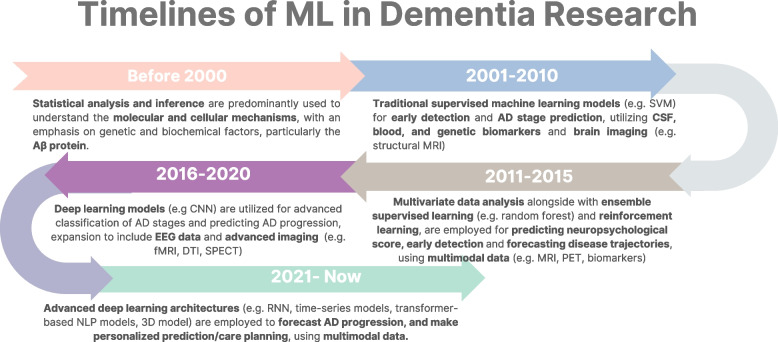
\includegraphics[width=\columnwidth]{figures/timelines-of-ml-in-dementia-research.jpg}
    \caption{Timelines of machine learning in dementia research. This figure is adapted from (Y. Wang et al., 2024, p. 175). Licensed under CC BY 4.0 (http://creativecommons.org/licenses/by/4.0/)}
    \label{ml-timelines}
\end{figure}

Although ML has shown promising results in research, the successful implementation of these ML-based solutions in clinical practice requires careful consideration of data-related challenges, such as ensuring high-quality, diverse, and representative datasets. In addition to addressing ethical concerns, it is crucial to establish robust validation to ensure that the solutions are accurate, reliable, and applicable in real-world settings. The application of ML in dementia prediction is evolving and will continue to grow as more diverse and high-quality data becomes available and the technical and ethical challenges are addressed. The following subsections provide a detailed review of different applications of ML models in CI and related disorders research.

\subsection{Prediction of Cognitive Impairment Using Machine Learning}
Early prediction helps to delay or prevent cognitive decline and promotes timely interventions. It also gives families time to organize support and resources \cite{Alzheimer2025}. Additionally, it may reduce the large social and economic burden on health systems. Recent advances in technology demonstrated that ML can effectively predict CI by analyzing huge amounts of diverse data. This subsection provides a summary of key trends, common challenges, and future research directions from recent reviews, offering a comprehensive overview of the current use of ML to predict CI and dementia.

A recent review systematically analyzed 100 related studies published between 2019 and 2022 \cite{Kaur2024Systematic}. The authors focused on specific types of data, such as Magnetic Resonance Imaging (\acrshort{MRI}), Positron Emission Tomography (\acrshort{PET}), genetic markers, and cerebrospinal fluid biomarkers. A key finding is the overwhelming popularity of DL strategies, which were used in about three-quarters of the studies. While there is an urge to use multi-data approaches, this review found that most researchers still rely on a single data type, specifically MRI scans. The Alzheimer’s Disease Neuroimaging Initiative (\acrshort{ADNI}) database stood out as the most common source of data; concurrently, the convolutional neural network (\acrshort{CNN}) algorithm emerged as the most used and highest-performing model. The review identified a significant gap, as most studies focus on classifying disease states (like Alzheimer’s disease (\acrshort{AD}) \acrshort{vs} healthy) rather than predicting the progression of CI. The paper also made a strong recommendation for researchers to move beyond the ADNI dataset, which would help to avoid bias.

A group of researchers reviewed the literature from the perspectives of doctors and biomedical scientists to provide an overview of ML's role in dementia research \cite{Wang2024Understanding}. They highlighted the history of the field from early genetic studies to today's advanced DL models that can forecast disease progression. This work explored unique methods from the last five years with a wide variety of data, covering simple questionnaires, complex brain imaging, and omics data. Despite the high performance achieved by some studies, serious limitations arise, such as data with missing values, a lack of standard methods for collecting data across different studies, and datasets that do not represent the full diversity of the population. The authors urged global initiatives to standardize the data and improve the clarity of the model predictions for clinicians. 

Another systematic review provides a comprehensive evaluation of automated dementia prediction systems \cite{Javeed2023Machine}. The review categorized studies published between 2011 and 2022 according to the types of data: images, clinical features, and voice recordings. From this modality-based comparison, the authors found that ML models trained on image data, like MRI scans from the ADNI and the Open Access Series of Imaging Studies (\acrshort{OASIS}) datasets, frequently produce better results for dementia prediction compared to models using clinical or voice data. Analyzing various ML techniques, supervised learning models are the most utilized, with SVM being the most frequently used classifier across all data types. Other commonly used classifiers are random forest and CNNs. This review found major problems with the current body of work, such as the possibility of model overfitting and the fact that most of the studies fail to handle imbalanced datasets. The author also highlighted inconsistent methods for training and testing models, which makes it difficult to perform fair comparisons between studies. The review recommends researchers to gather larger and more robust datasets, particularly for voice and clinical-feature analysis, and explore multimodal approaches that combine different data types to create more reliable and efficient prediction models. Similar findings and conclusions were provided by another systematic review \cite{Arya2023systematic}, which encourages reducing the dependence on a single dataset and suggests exploring more diverse data types and combining different models using ensemble techniques.

While most of the reports focus on solutions based on high-cost data, a recent systematic review discussed the potential of automated cognitive assessment using non-neuroimaging data \cite{Babatope2024Potential}. The review selected 87 studies that did not use expensive brain scans like MRI or PET and were published between January 2000 and June 2024. The review concluded that automated tools can produce a comparable level of performance and outperform conventional methods in some studies. To build trust and encourage the adoption of these tools, the authors recommend more collaboration between technology developers and medical experts. 

In a similar context, a more recent review looked at 60 peer-reviewed articles on non-invasive CI detection \cite{Alsuhaibani2025Review}. This review pointed out that models based on speech and language analysis are as effective as those based on costly medical imaging. However, making these automated and low-cost solutions available in low-income regions remains a challenge. Future studies should understand and overcome the barriers that prevent their use in underserved populations worldwide.

Based on this board view of the literature, it can be noticed that there is a clear need for more research and development in the prediction of CI using ML to create affordable and accessible solutions. The following subsections discuss in more detail how different data types are used in the literature to develop ML models for CI and dementia.

\subsubsection{Cognitive Impairment Prediction Using Neuroimaging Data}

Neuroimaging data, such as MRI and PET, are widely used in dementia research. These data offer large shared repositories for training models and contain high-dimensional patterns for analysis. The application of ML in neuroimaging for dementia diagnosis was the subject of a systematic review that surveyed 255 studies \cite{Borchert2023Artificial}. This research area has grown quickly since 2017. This growth coincides with a shift from simpler SVM models to more complex neural networks. This could be related to the introduction of the Transformer architecture in 2017 \cite{Vaswani2017Attention}, which brought scalable attention-based modeling and made it easier to train large, flexible networks on complex data. A great variation in model performance was observed. For instance, the diagnostic accuracy for AD ranged widely from 60.2\% to 99.3\%. Meanwhile, a narrative review paper explored the role of AI and ML in the use of neuroimaging to predict early AD \cite{Rudroff2024AI}. The studies showed a common pattern of use, as CNNs were typically utilized for image analysis, while RNNs were applied to longitudinal data. The review noted a high overall performance. Some frameworks achieved 93\% accuracy in classifying AD and 82\% accuracy in predicting MCI-to-AD conversion by using multi-modal DL.

A systematic review with a meta-analysis focused on the use of multimodal neuroimaging data with ML to classify AD stages \cite{Odusami2024Machine}. The review included 47 studies from 2016 to 2022. Among the different methods, supervised learning algorithms were identified as the most common approach. The authors also highlighted the use of feature-level fusion as a popular strategy to combine various data types from different sources. As a result,  model performance was improved through the use of multimodal neuroimaging data. For classifying AD, the sensitivity was 94.6\% and the specificity 93.5\%. However, the performance in distinguishing progressive from stable MCI was lower, with sensitivity and specificity at 80.4\% and 81.4\%, respectively.

The reviews commonly observed a dominant use of certain brain scans (MRI and PET) and a heavy reliance on the ADNI dataset. Limitations in the reviewed studies were also highlighted, particularly the absence of external validation and the lack of explanation of complex models. The authors suggested several priorities for future studies, including validating models on external datasets, using methods to make AI decisions more transparent, and expanding research into under-studied areas like non-AD dementias.

A group of researchers has developed a DL model for the differentiation of normal cognition, MCI, AD, and non-AD dementias \cite{Qiu2022Multimodal}. They employed a mixed method analysis of data from eight cohorts for developing and testing various models in a multimodal manner. These included an MRI-only CNN, traditional ML classifiers, and a fusion model that combined imaging and non-imaging data. The models showed high diagnostic performance, which is almost equal to that of expert neurologists or neuroradiologists. 

Several studies employed advanced methodologies and neuroimaging data to achieve different objectives. To classify Parkinson’s disease (\acrshort{PD}) using Single-Photon Emission Computed Tomography (SPECT) images, one study proposed a soft attention-based DenseNet model \cite{Thakur2022Soft}. The DenseNet-121 architecture with a soft attention block was used to enhance attention in relevant areas of the brain. The proposed model outperformed previous studies by achieving a high accuracy of 99.2\%. \citeA{Lim2022Deep} built a DL model for early AD diagnosis using structural MRI (\acrshort{sMRI}) data. sMRI scans were preprocessed to remove the skull, correct for the bias field, segment images into tissues, and extract 2D slices from 3D MRI volumes. To overcome the problem of overfitting a small dataset, the authors augmented the data by rotating and zooming the images. The preprocessed images were then used to train and evaluate three CNN models: CNN from scratch, VGG16, and ResNet-50. The VGG16 and ResNet-50 models used transfer learning by initializing the weights with ImageNet pre-trained weights. The VGG16 model produced the most accurate performance of approximately 79\%. Another group of researchers addressed the same problem using a novel DL framework for the classification of early-stage AD based on brain MRI images \cite{Hazarika2023Novel}. The authors employed 3D MPRAGE MRI scans from the ADNI dataset and extracted 2D slices from the hippocampal region. The authors proposed a modified VGG-199 model with Dense and Inception blocks to reduce the number of parameters by 21\%. They then used the Principal Component Analysis (\acrshort{PCA}) to retain 88\% of the original features while retaining 100\% variance. Finally, the classification of cognitively normal, early-stage AD, and AD subjects was performed using a random forest classifier. This method outperformed several state-of-the-art methods with a high classification accuracy of approximately 98\%. The outcomes of these studies prove the possibility of the early diagnosis of CI using brain scans. However, the authors highlighted limitations due to data scarcity and suggested the use of more extensive and diverse datasets, incorporation of multimodal data, and exploration of 3D CNN architectures to improve the model's generalizability and robustness.

A multi-modal approach that combines 3D MRI and amyloid PET scans was implemented to improve AD detection \cite{Castellano2024Automated}. After evaluating different variations of CNN architectures and imaging dimensionalities, parallel processing of multi-modal scans using the dual-branch fusion model achieved the highest results of 95\% accuracy. To address challenges in the early diagnosis of AD from 18F fluorodeoxyglucose (\acrshort{FDG}) PET scans, another paper introduces a novel DL model named ResGLPyramid \cite{Rehman2024Early}. The model is built of a combination of a Tri-Convolutional-Transformer and an attention module. This design allows the model to capture local details and global context from the brain images. The model scored a 92.75\% accuracy and a 0.925 area under the curve (\acrshort{AUC}) for classifying AD and MCI.

Systems based on MRI and PET scans could be used to accurately detect CI. However, the cost and the need for specific equipment and skills prevent many people from accessing these tools \cite{Geethanath2019Accessible}. Researchers have explored the use of electroencephalograms (EEGs) as alternative brain scans to predict CI with ML. EEG is an inexpensive and portable neuroimaging method compared to other methods, such as MRI. Resting state EEG and sMRI were compared in order to differentiate between AD and MCI using low-cost approaches \cite{Farina2020Comparison}. The EEG markers used are frequency band power and functional connectivity. Compared to sMRI, AD classification using EEG achieved a higher accuracy of 70\% with a sensitivity of 74\% and a specificity of 64\%. However, both techniques demonstrated moderate accuracy in differentiating MCI from healthy controls.

A recent review discussed how EEG is used as a diagnostic tool for AD between 2000 and 2023 \cite{Ehteshamzad2024Assessing}. The review found a clear progression. This progression was from traditional visual inspection of EEG to automated analyzes using quantitative EEG (qEEG) and ML. EEG can detect minor functional brain changes much earlier than the structural changes that might appear on MRI or PET scans. Another methodological analysis found that 85\% of studies use EEG signals to detect AD rather than early prediction \cite{Modir2023Systematic}. Additionally, the majority of the studies are using ML classifiers like SVM. These modern approaches can achieve high diagnostic sensitivity and specificity rates above 85\%. The use of EEG signals with more complex models (DL models) for the detection of AD and MCI was recently reviewed \cite{Acharya2025Deep}. The review noted an increase in publications since 2022. This could be driven by the effectiveness of CNNs and transfer learning models like ResNet, which achieved outstanding performance. The use of small datasets and the lack of standardization in EEG protocols are the main methodological gaps highlighted in all reviews.

Access to this effective technology is challenging in LMICs due to the lack of expertise and digital infrastructure. A recent systematic review discussed the potential of automated cognitive assessment approaches that do not rely on neuroimaging data \cite{Babatope2024Potential}. The review included 87 studies that utilized game-based tools, digitized versions of conventional tests, original computerized batteries, virtual reality or smart home systems, and artificial intelligence-based methods. The potential of these non-neuroimaging approaches can be observed from the achieved comparable performance of greater than 80\%. The following subsections provide a review of the application of other effective and more accessible data types in CI prediction.

\subsubsection{Cognitive Impairment Prediction Based on Activity Recognition}
With advances in technology, several automated and noninvasive methods have been developed to predict CI. Activity recognition in intelligent environments, such as smart homes, has been utilized to monitor patient activities to predict CI patterns \cite{Khan2021Prediction}. Digital biomarkers captured by specific human body functions and tasks, such as eye tracking, handwriting, speech, and gaming, have also been employed in dementia prediction research \cite{Ding2022Digital}. 

A recently published systematic review analyzed 72 studies published between 2012 and 2022 that used DL for the diagnosis of dementia using speech and language data \cite{Shi2023Speech}. The review found that many studies have been published in this research domain after 2020. Studies in this field commonly use the DementiaBank dataset. They also often use feature extraction with DL embeddings like Bidirectional Encoder Representations from Transformers (\acrshort{BERT}). The reviewed studies reported high classification accuracies between 80\% and 90\% to classify dementia patients from healthy controls, with some reaching as high as 97\%. In addition to speech processing, \citeA{Alsuhaibani2025Review} reviewed 60 studies that used DL to find CI using non-invasive signs like language, speech, facial expressions, and motor mobility as less expensive alternatives to neuroimaging. Speech- and language-based methods generally achieve the highest detection performance, especially when they combine acoustic and linguistic features. These methods depend a lot on transfer learning with pre-trained models like BERT for linguistic analysis and CNNs or vision transformers for visual data. These reviews pointed out critical gaps that could impact the clinical adoption of these solutions. For instance, large and balanced datasets are limited and standardized data collection methods and model explainability are not applied.

A comparison of speech and gait analysis methods was the focus of another systematic review \cite{Al-Hammadi2024Machine}. It examined 40 studies published from 2017 to 2022. This paper highlighted that SVM was the most common method, followed by DL approaches. This contradicts the heavy focus on DL in other reviews. It was also found that better accuracy can be obtained by analyzing the gait features of the entire body. Future work should explore multimodal approaches (such as fusing gait and speech data) and more diverse languages and longitudinal study designs.

Several studies used natural language processing (\acrshort{NLP}) for the early detection of CI. For instance, \citeA{Amini2024Prediction} developed a new method to predict the progression of MCI to AD within a time frame of 6 years based on speech data and NLP. The approach included three main components: an automated speech-to-text pipeline, a transformer-based sentence encoder to generate embeddings, and finally logistic regression models for prediction. The proposed approach was found to be more accurate than traditional neuropsychological tests and other noninvasive approaches. Other researchers have investigated the optimization of this approach using GPT embeddings \cite{Runde2024Optimization}. The results demonstrated that the transcriptions performed by AI services had better accuracy and F1-score than manual transcriptions. The study showed that NLP can accurately identify AD. However, it was less effective in detecting possible AD and MCI. The authors believe this was due to limited training data.

Looking at different types of digital biomarkers, \citeA{Pavisic2017Eyetracking} built an ML classifier with 95\% accuracy to diagnose early-onset Alzheimer’s using data collected from eye-tracking experiments. In addition, \citeA{Opwonya2023Eye} explored the potential of eye movement data and a multimodal approach to identify MCI in a cost-effective manner. Researchers have built ML models that incorporate eye movement metrics, demographic information, and cognitive scores. While acknowledging limitations in generalizability and the need for further validation, the authors propose this method as a promising, noninvasive, and cost-effective MCI screening solution. As an advance of this approach, \citeA{Alsuhaibani2024Mild} introduced a DL model for the identification of MCI in an early stage based on facial and interaction features obtained from video recordings of patient interviews. The method includes a convolutional autoencoder that extracts holistic spatial facial features from individual frames and a Spatial-to-Temporal Attention Module that captures temporal information and interaction dynamics across video sequences and segments. The framework had an accuracy of 88\% in differentiating MCI from participants with normal cognition, but had the drawbacks of manual video quality assessment and a relatively small dataset.

Using a different approach, another group of researchers developed a novel model to automatically detect dementia based on the dynamics of the handwriting process \cite{Angelillo2019Attentional}. \citeA{Carina2023Handwriting} conducted a systematic review and found that people with AD struggle with various aspects of handwriting. Their review revealed that patients have more trouble with understanding where to place letters on paper and expressing their thoughts through writing compared to simple motor issues. Although the model provides an accurate, cost-effective, and convenient diagnostic solution, its generalizability remains questionable.

In later work, \citeA{Uddalak2024ML-Powered} aimed to detect AD early by utilizing ML to analyze handwriting and take advantage of the effects of AD on fine motor control. Several base classifiers are integrated using the stacking technique to create an ensemble model. The ensemble model was trained on a dataset of handwriting samples gathered from 89 AD and 85 healthy participants. The ensemble model achieved high performance with a 97.44\% F1-score, outperforming the state-of-the-art models on the same dataset. The outcome highlights the considerable clinical utility of ML for highly accurate, cost-effective, and non-invasive prediction of AD through handwriting analysis. 

Other researchers have developed gamified assessment tools to simplify and accelerate cognitive assessment. According to a recent scoping review \cite{Chen2025Video}, these systems demonstrated diagnostic performance comparable to traditional screening tools like the Montreal Cognitive Assessment. In a recent study, \citeA{John2023Development} investigated how ML classifiers could predict cognitive function using head kinematic data from virtual reality exergames. The participants were older adults, and the study took place over a period of six weeks. The classifiers successfully identified correlations between the kinematics of head movement and cognitive performance measures. The findings of this study suggested that virtual reality head movements captured from games can be used as a digital biomarker to assess cognitive status. Gamified systems are engaging and can be used for home monitoring. However, it has been revealed that current research in this area has methodological issues related to small sample sizes and a lack of robust validation methods to assess how these systems work over time \cite{Chen2025Video}.

Although studies leveraging body functions and digital biomarkers offer fully automated, noninvasive, and cost-effective methods for CI and dementia assessments, future work may involve validating the models in larger and more diverse populations and exploring the incorporation of other biomarkers for improved accuracy. Furthermore, the application of these methods may require a certain level of user knowledge, the utilization of specific equipment, and modifications to the patient's environment. These requirements make these solutions impractical and less desirable for conducting highly scalable CI assessments.

\subsubsection{Cognitive Impairment Prediction Using Clinical Notes Analysis}

Examining patterns in clinical notes could be effective in detecting CI. This was the finding of a systematic review of 18 studies using NLP models \cite{Shankar2025Natural}. The review highlighted that the models achieved higher results than rule-based algorithms and traditional ML models. A group of researchers explored using NLP to analyze clinical notes of approximately four thousand patients in two cohorts \cite{Penfold2022Development}. They developed 42 cognitive-related concepts through manual annotation of over 10,000 notes. Using \acrshort{LASSO} regression, the model achieved moderate performance with an AUC of 0.67. The researchers needed to manually label huge amounts of data and set up complex NLP systems to implement their approach. \citeA{Laurentiev2023Identifying} examined how NLP could extract information about daily functioning from digital medical records of people with dementia. Their cross-sectional study developed ML models using clinical note text to identify activities of daily living impairments among 441 older adults with dementia. Random forest and SVM models achieved high AUC scores above 0.97. However, the main limitation was that researchers had to manually annotate thousands of notes and rely on specialists to select relevant keywords for filtering.

A recent study used large language models (\acrshort{LLMs}) to detect cognitive decline from available clinical notes in the EHR \cite{Du2024Enhancing}. In this study, annotated note sections from 6,945 clinical documents related to 2,166 patients were used. The researchers tested how GPT-4 and Llama 2 performed compared to traditional ML models. Although GPT-4 performed better than Llama 2, traditional ML approaches performed better than both LLMs. The performance of an ensemble model combining all models (0.921 F1-score) was higher than the performance of an individual model (0.854 F1-score). In a different study, \citeA{Amini2024From} used a transformer-based Universal Sentence Encoder to analyze clinical notes from Massachusetts General Brigham's EHRs. Using two sampling strategies, they achieved outstanding results in distinguishing normal cognition from dementia (0.978 AUC) and moderate performance for normal cognition versus MCI (0.81 AUC). While demonstrating encouraging outcomes, their approach required extensive computational infrastructure and specialized NLP expertise. In addition, these methods depend on very complex text processing and transformer models.

Analyzing patterns in clinical notes offers an automated and non-invasive approach to detect CI and dementia-related disorders. However, studies in this domain have limitations, including heterogeneity in performance metrics and limited external validation across diverse populations \cite{Shankar2025Natural}. Another limitation is that these methods necessitate extensive annotation and complex programs to process text. To overcome these challenges, there is a need to develop more cost-effective methods to use clinical notes analysis in real clinical settings \cite{Shankar2025Natural}.

\subsubsection{Cognitive Impairment Prediction Using Neuropsychological and Cognitive Tests}
The literature has extensively analyzed in various ways the use of neuropsychological tests and cognitive scores as noninvasive and cost-effective predictors of CI. A group of researchers compared the efficacy of molecular and radiological biomarkers and neurocognitive assessments in predicting the progression from MCI to AD \cite{Daou2023Can}. The accuracy of both methods appears to be inconsistent. This variation is likely influenced by which tests are selected and also by the characteristics of the sample. Valuable insights came from biomarkers. However, neurocognitive assessments presented themselves as an alternative that is more accessible and has a lower cost. This was especially true when tests for memory, executive function, or language were combined. A focus for future research, as suggested by the authors, should be on accessibility and cost.

A systematic review examined 37 studies on AI and ML that were used for the evaluation of MCI and dementia \cite{Veneziani2024Applications}. \citeauthor{Veneziani2024Applications} found three main areas where AI could be very useful. The study suggests that AI can help improve traditional assessments, select effective tests, and create new evaluation methods using virtual reality. It appears that ML algorithms, for example, SVM and DL, were more effective than conventional assessment tools. Some mobile screening tests were found to be better than the standard Montreal Cognitive Assessment, and automated systems for semantic verbal fluency showed a high correlation with manual scoring. The review also highlighted other newly developed technologies, such as game-based and virtual reality tests. However, some important problems remain. Most of the studies were based on the ADNI database, which raises concerns about generalizability. A gap was also noted between technical success and clinical utility in the real-world. The tools should be useful to clinicians to simplify workflow rather than being computationally advanced.

In a previous study, \citeA{Grassi2019Novel} worked to develop an ML algorithm to predict the conversion from MCI to AD. It used different available data, such as demographic characteristics, clinical information, and neuropsychological test scores. The algorithm achieved an AUC of 0.88, which indicates a high accuracy in predicting dementia. The algorithm presented a cost-effective solution depending only on non-invasive and affordable measures. In another work, \citeA{El-Sappagh2021Alzheimers} explored cost-effective approaches to predict the progression of AD using ML. They compared five algorithms trained on multimodal time-series data from the ADNI dataset, including demographic data, cognitive scores, and medication history. The researchers made an important breakthrough by incorporating semantically encoded comorbidity and medication features into their early fusion approach, significantly improving the accuracy of prediction. 

Using ML, \citeA{Alshboul2023Application} studied how to use non-invasive indicators for dementia diagnosis. Their study looked at the ADNI dataset. It focused on factors such as Clinical Dementia Rating (\acrshort{CDR}) scores and demographics. The authors found that ML models could accurately classify patients with dementia. This result shows the potential of low-cost cognitive tests in helping clinicians make an efficient diagnosis. In another study, \citeA{Kim2024Using} tried to develop cost-effective screening tools for cognitive decline using neuropsychological assessments. The researchers analyzed 2,863 subjects with cognitive complaints. All subjects completed the Seoul Neuropsychological Screening Battery, which covers five cognitive areas. The researchers trained a random forest classifier. The goal was to identify the most predictive test combinations for distinguishing between dementia and non-dementia cases. The model's performance was 82.42\% accuracy and had a 0.816 AUC score.

Some researchers investigated ways to make the predictions of the model more transparent. This study explored a methodology to create an efficient and explainable tool for predicting the onset of dementia within three years \cite{Beebe-Wang2021Efficient}. The research analyzed longitudinal clinical and cognitive information across multiple domains. The analysis revealed that data from a single recent visit was enough for an accurate prediction, without the need for years of historical data. Model explainability was a key focus, with the SHapley Additive exPlanations (\acrshort{SHAP}) method used to select a small group of highly predictive cognitive tests and also to provide personalized risk explanations for each person. The final simplified eXtreme Gradient Boosting (\acrshort{XGBoost}) model, which used only four short cognitive tests, achieved a test AUC of 0.89. This performance is comparable to using the entire neuropsychological battery. \citeA{Basta2023Personalized} introduced an ML framework designed for personalized screening for MCI in primary healthcare settings. The study used demographic, clinical, behavioral, and Mini-Mental State Examination (\acrshort{MMSE}) data gathered from 763 older adults. The participants were categorized as 277 with MCI, 153 with dementia, and 333 showed no CI. Since the classes are not balanced, a balanced random forest classifier was trained using a nested cross-validation approach to ensure reliable results. To interpret the reasoning of the model, the researcher employed model-agnostic explainability techniques at the group and individual levels. The framework achieved fair performance in distinguishing cognitively healthy participants from those with MCI, with a sensitivity of 74\%. This result was a clear improvement compared to using MMSE alone, which reached only 37.2\% sensitivity. This result shows that it is valuable to integrate readily accessible primary care data with MMSE scores.

The creation of a highly accurate and interpretable ML model for the early prediction of AD was also the objective of a recently published study \cite{Hossain2025Optimizing}. A publicly available Kaggle dataset was used that contained clinical and lifestyle data from 2,149 adults. The features covered a wide range, from demographics and lifestyle to cognitive assessments (including MMSE) and cognitive symptom reports. The researchers developed a stacked ensemble model. This model first combined predictions from the gradient boosting and XGBoost models. Then, a logistic regression model was used to make the final classification of AD versus non-AD. A very high level of performance was achieved, with the final stacked model showing 97\% accuracy and an AUC of 0.97. The SHAP method was essential for the interpretability of the model. It helped to clarify the influence of each feature on the model's output. This work suggests that an ensemble approach can provide excellent predictive performance. In addition, SHAP provides the transparency that is needed for clinical application. However, the study is limited by its use of a single cross-sectional dataset and the model may not generalize to other populations without further validation in diverse datasets. Another study presented similar findings using a comparable group of features taken from the same Kaggle dataset \cite{Mahamud2025Enhancing}. In this research, the authors applied the Synthetic Minority Over-sampling Technique (\acrshort{SMOTE}) to handle class imbalance. They also used Chi-Square and Recursive Feature Elimination (\acrshort{RFE}) methods to select the most relevant features. Moreover, SHAP and Local Interpretable Model-agnostic Explanations (\acrshort{LIME}) techniques were used to explain how the model made its predictions.

ML models trained in neuropsychological assessments and cognitive test scores are often seen as a non-invasive and more affordable solution. However, it is important to note that these assessments may need trained examiners to administer them. They may also show cultural \cite{Puente2015Neuropsychological} or educational biases \cite{Noroozian2014Impact}. These problems limit how widely they can be accessed and how effective they are as routine assessments. For this reason, the clinical use of neuropsychological assessments requires more effort. These efforts are needed to establish standardized processes \cite{Alzola2024Neuropsychological}.

\subsubsection{Cognitive Impairment Prediction Using Routine Clinical Data}
\label{sec:similar-studies}
In light of the constraints that exist in current non-invasive and automated approaches, scholars have explored other accessible and cost-effective solutions for screening and predicting the onset of CI and dementia. This section discussed recent studies that investigated whether low-cost clinical data collected during regular medical treatment, such as sociodemographic, lifestyle, and health measures, could effectively predict dementia compared to higher-cost assessments. Table~\ref{table:ci-review} provides an overview of the reviewed studies, including utilized datasets and features, modeling approaches, and obtained results.

A related study evaluated the accuracy of accessible clinical data from the National Alzheimer’s Coordinating Center (\acrshort{NACC}) to diagnose and predict AD progression \cite{Ren2023Improving}. The researchers created a framework that organized the data according to its level of accessibility. The data were divided into three groups: low-cost data from primary care, medium-cost data from specialist visits, and high-cost data available only in research settings. The primary care data consisted of demographic details, patient medical history, results of physical examinations, and responses to questionnaires. They trained hierarchical and ensemble ML models in the primary care data to distinguish between cognitively normal, MCI, and AD diagnoses. The multiclass random forest model achieved 0.773 accuracy, which improved to 0.815 in hierarchical classification. In a later study, the same group of researchers applied a similar data categorization with semi-supervised ML \cite{Ren2025Identifying}. The researchers gathered data on 4,014 participants from NACC and 36,621 participants from the \hl{generalized dataset}. They categorized the features into three tiers: low-cost (demographics, behavioral surveys, basic assessments), medium-cost (neuropsychological testing), and high-cost (clinical dementia rating (CDR), genetic testing). Low-cost features with longitudinal data achieved an AUC of 0.719 to predict neuropathological cases. The result was comparable to higher-cost single-visit approaches. The key low-cost predictors included the geriatric depression scale, functional assessment measures, and medication patterns. The outcome of these studies demonstrates that accessible, cost-effective clinical data can be used effectively to detect CI. However, the need for longitudinal data collection could limit the application of these models in real-world settings with restricted access to historical data.

Diverse ML and DL algorithms with readily available and easily accessible health records have been evaluated for the classification of CI. \citeA{Li2023Machine} developed predictive ML models using accessible clinical data for CI among 2,226 participants between 60 and 80 years of age. Only 384 (17.25\%) of the participants were diagnosed with CI. The researchers constructed a composite Z-score for cognitive functioning through four standardized tests. They also included 13 affordable demographic, lifestyle, and clinical features like the dietary inflammatory index, glycated hemoglobin, PHQ-9 depression scores, sleep duration, and albumin levels. Then, ten important features were selected using the Boruta algorithm. They used these features to train a generalized linear model (\acrshort{GLM}), random forest, SVM, artificial neural networks, and stochastic gradient boosting models. The models were trained with 10-fold cross-validation on a 70-30 train-test split. The GLM resulted in the highest performance with an AUC of 0.779. The authors noted a lack of external validation and a lack of family history data. \citeA{Cui2024Prediction} conducted a similar study to develop CI classification models based on accessible data from the Chinese Longitudinal Healthy Longevity Survey. The data were divided into a development dataset of 2,138 participants and two external validation datasets of 501 and 746 participants. The researchers used LASSO regression to select features from a set of 34 features. The initial feature set consisted of health and lifestyle data in addition to activities of daily living (\acrshort{ADL}) and instrumental ADL (\acrshort{IADL}) scores. The researchers evaluated logistic regression, SVM, random forest, and XGBoost using 10-fold cross-validation. Logistic regression outperformed the other models with 0.778 accuracy and 0.875 AUC. Further validation in public health practice is needed to confirm the generalizability of the developed models.

In recent years, researchers have been exploring different ways to use accessible data and ML to create affordable screening tools for dementia and related disorders. A study developed a random forest model to predict dementia using both structural and non-structural data from the Electronic Medical Record (\acrshort{EMR}) collected from several healthcare institutions \cite{Ben2020Predicting}. The model reached an accuracy of 0.80 and was described as a non-invasive and cost-effective method to identify the risk of dementia among general patients. A proof-of-concept study compared ML algorithms versus traditional statistical methods for dementia prediction at a 12-year follow-up \cite{Twait2023Dementia}. \citeauthor{Twait2023Dementia} used clinically accessible data from 4,793 participants. The utilized features are demographic data, clinical variables, lifestyle factors, MMSE, and medication. The researchers evaluated elastic net regression, random forest, SVM, and logistic regression models on three different sets of features. These sets are all features, features after Boruta feature selection, and clinically accessible features (excluding MRI features). All models produced similar levels of performance, but the elastic net regression model was better than the other models considering the balance between the sensitivity and specificity scores. The authors highlighted a potential overfitting because assessments used for dementia, such as the MMSE, are also used as input features.

A novel framework based on a transfer learning paradigm was proposed with the objective of creating an explainable and personalized model for predicting dementia risk \cite{Danso2021Developing}. For this, a source model was first trained with data from the large SHARE study, which included 84,856 older individuals. The knowledge of this model was then transferred and its decision boundaries were updated using data from a younger and undiagnosed population of 473 individuals in the PREVENT study. Sociodemographic information, medical history, and lifestyle details served as input features. For model explainability, SHAP was applied to visualize the risk factors responsible for prediction at both the population and individual levels. The research evaluated random forest and XGBoost algorithms and found that XGBoost was better at predicting AD versus non-AD status in the source model, with an AUC of 96\%. The final target model achieved an AUC of 63\% for predicting high-risk versus low-risk status. The performance of the final model could be affected by the small size of the sample from the PREVENT study.

Multiple studies have evaluated the development of ML models based on accessible data, such as EHRs, for the early prediction of dementia multiple years before disease diagnosis. \citeA{Nori2019Machine} developed a gradient-boosting machine model using data from administrative and EHR sources to predict the onset of dementia from 3 to 8 years. A low sensitivity of 0.47 was achieved by the model in the third year, which dropped to 0.15 in year 8. In a similar study, \citeA{Park2020Machine} employed large-scale administrative health data to predict definite and probable incident AD within 1 to 4 years. The study utilized a nationwide population-based cohort of subjects above 65 years. The predictive models produced a reasonable range of AUC values ranging from 0.644 to 0.775.

Recent studies have explored the use of EHRs to predict Alzheimer’s disease and related dementias (\acrshort{ADRD}) one to five years before diagnosis. This includes a recent development of ML models using data from 23,835 patients and more than a million control patients \cite{Li2023Early}. Data included basic demographic details, medical diagnoses, prescriptions, laboratory test results, and vital signs.  The study examined two approaches, which are knowledge-driven features selected by domain experts and data-driven approaches using all available variables. Logistic regression and gradient boosting tree (\acrshort{GBT}) models were trained on both approaches and tested across different prediction windows. They achieved AUC scores of 0.939 for the 0-year window, 0.906 for 1 year, 0.884 for 3 years, and 0.854 for 5 years before diagnosis. However, the method of this study has critical limitations, like sample selection bias and the absence of external validation. A similar study used EHR data from the University of Missouri Healthcare, consisting of 4,012 ADRD cases and 119,723 controls \cite{Akter2025Using}. The dataset included demographic information, behavioral risk factors, vital signs, and several common comorbidities. The team tested six ML methods: GBT, \acrshort{LightGBM}, XGBoost, random forest, logistic regression, and AdaBoost. Among these, the GBT model performed the best. Its AUC scores were 0.809 for the 1-year window, 0.821 for 2 years, 0.822 for 3 years, 0.808 for 4 years, and 0.833 for the 5-year window before diagnosis. It is worth noting that performance showed an improvement with longer prediction windows, which could indicate that using a wider range of historical datasets improved accuracy. However, the performance of the models on other healthcare systems or populations remains questionable because a generalizability test was not performed in this study.

Other studies aimed to predict dementia with a longer prediction period. A longitudinal retrospective cohort study developed ML models to predict incident dementia in 5, 10, and 13-year prediction windows using routinely collected primary and secondary care EHRs \cite{Georgiev2024Predicting}. The study included 144,113 senior adults aged 50 to 102 years in Scotland. Participants were dementia-free prior to 2009 and had follow-ups until 2023. Only 8\% of the participants developed dementia over the period of 13 years. The researchers employed data-driven and clinically supervised feature approaches, including age, deprivation indices, lifestyle factors, modified electronic frailty index, cardiovascular risk scores, laboratory tests, and chronic conditions. XGBoost models were trained using 70-30 random stratified splits with 10-fold cross-validation. Data-driven models achieved slightly higher AUC scores of 0.888, 0.866, and 0.847 at 5, 10, and 13 years, respectively, compared to clinically supervised models. However, the models resulted in lower sensitivity scores below 0.756. For future work, the author suggested externally validating the model to evaluate its generalizability.

Researchers have also applied ML to classify different stages of CI using accessible data. \citeA{Zhu2020Machine} used records from 5,272 participants recruited in hospitals across Taiwan to distinguish four stages: normal cognition, MCI, very mild dementia (\acrshort{VMD}), and dementia. Data were gathered with a 37-item questionnaire that covered demographic information, cognitive tests, measures of daily functioning, and neuropsychiatric symptoms. The researchers compared three feature selection methods, namely information gain, Relief, and random forest. They also evaluated six different ML models. Using information gain for feature selection together with a Naive Bayes classifier produced the best results, yielding an overall F1-score of 0.81 for multiclassification. Stage-specific F1-scores were 0.67 for normal cognition, 0.68 for MCI, 0.71 for VMD, and 0.93 for dementia. In a related study, \citeA{Vyas2022Identifying} trained binary classifiers to detect dementia and multiclass models to classify its severity. This work relied on demographic profiles, cognitive assessment scores, and clinical parameters. To ensure high modeling quality, dementia experts performed data curation. The researchers evaluated random forest and decision tree algorithms with stratified cross-validation. The random forest model achieved the highest F1-scores of 0.93 for binary classification and 0.81 for severity classification.

The following studies approached the classification of multiple CI stages using multiple binary classification models. This study presented an explainable ML approach for predicting MCI and AD \cite{Yue2023Explainable}. The work utilized data from 2,658 participants in the China Longitudinal Aging Study (\acrshort{CLAS}). A wide range of features were used from categories like demographics, daily lifestyle, medical history, and physical examinations. The modeling process involved handling data imbalance with the \acrshort{ADASYN} (Adaptive Synthetic Sampling Approach for Imbalanced) oversampling technique and comparing five methods for feature engineering, ultimately using ReliefF to select 15 key features. To understand the model's decisions, the SHAP method was utilized to visualize each feature's contribution to the prediction at both global and individual levels. AdaBoost was selected as the best model after evaluating nine different classifiers using 10-fold cross-validation. The model performed two separate classification tasks: normal cognition (\acrshort{NC}) versus MCI and NC versus AD. For MCI/NC prediction, the model achieved an accuracy of 89.2\%, while for AD/NC prediction, the accuracy was 99.2\%.

ML models were developed for predicting MCI and dementia onset using accessible sociodemographic and health-related features from the Korean Longitudinal Study of Aging \cite{Oh2024Multivariable}. The research work included 4,975 older adults aged 60 years or older. Out of these participants, 23 developed MCI and 70 developed dementia. The researchers compared nine ML algorithms and addressed class imbalance using weighting mechanisms. The random forest model achieved the best performance for the prediction of MCI (AUC of 0.673), while XGBoost produced the highest results for the prediction of dementia (AUC of 0.819). Another group of researchers established a similar approach using EHR data from the John Paul II Geriatric Hospital in Poland \cite{Richter2025Cognitive}. The data consisted of 144 individuals with MCI, 38 with dementia, and 101 healthy controls. The study utilized cost-effective features, including sociodemographic variables, laboratory test results, comorbidities, BMI, and functional scales. The researchers evaluated ten ML algorithms after applying \acrshort{ANOVA} for feature selection and SMOTE to balance the training data. For MCI versus control classification, the non-linear SVM model scored the highest performance with 0.69 accuracy and 0.75 AUC. For dementia versus control classification, the random forest model demonstrated high results with 0.84 accuracy and 0.96 AUC. The performance of the binary classification models in both studies highlights that classifying MCI cases is much harder than classifying dementia cases. Additionally, the generalizability of these models is limited by the small data size and retrieval of data from a single research center.

Accessible data from the NACC dataset were used by several studies to classify and predict CI. In a previous study, \citeA{Wang2018Early} compared the accuracy of different ML models for the early detection of AD. The models that were tested included feed-forward and Bayesian neural networks, tree-based algorithms, and long short-term memory (\acrshort{LSTM}). Data came from 6,269 NACC subjects. These subjects had probable AD, and conducted between 2 and 12 visits. The LSTM model achieved an average accuracy of 0.835. This score outperforms the other models by 5\%. In their other study \cite{Wang2018Predictive}, \citeauthor{Wang2018Predictive} utilized the historical medical record of the NACC dataset to develop an LSTM model to predict AD status in the next medical visits. The global CDR score was used to define five different AD stages. The results showed that the proposed approach significantly outperformed the classic baseline methods. These studies demonstrated the potential of recurrent neural networks in producing accurate and reliable models by effectively utilizing the temporal and medical patterns extracted from past patient visits. \hl{In a recent study, a deep learning model was developed on longitudinal data from the ADNI dataset to predict cognitive conversion at different years after the baseline, reaching AUC scores between 0.87 and 0.92, while simpler models that rely on fewer variable sets maintained an AUC above 0.80} \cite{Yang2025Prediction}.

Another study also utilized the NACC dataset and ML models to develop a low-cost screening tool for AD trials \cite{Pang2023Predicting}. The tool is designed based on readily available clinical data to predict the transitions from unimpaired to MCI and from MCI to AD. The researchers evaluated different models and feature selection techniques and eventually identified a group of 20 clinical variables that provided precise predictions. The main outcome of their study is a calculator that is easy to use based on the selected variables. The calculator offers a cost-effective and accessible approach to pre-screening trial participants. Another study approached the progression from MCI to dementia differently \cite{Bucholc2023Hybrid}. The authors developed a two-stage framework. This framework utilized cost-effective and non-invasive cognitive scores from the NACC dataset. In the first stage, distinct cognitive decline trajectories were identified using unsupervised learning. The optimal number of clusters was determined using multiple clustering validity indices and fusion-based methods. These trajectories were then incorporated into supervised ML models in the second stage. As a result, an improvement of 6\% in prediction accuracy was observed, compared to models that only rely on clinical scores. This framework achieved an accuracy of 0.875. This was for predicting dementia conversion using data from four time points. \citeA{abbas2024Explainable} recently utilized data from ADNI to externally validate ML models for the classification and prediction of three cognitive stages. The models were trained using demographic, health history, and cognitive assessment features from the NACC dataset. Using Boruta-based feature selection, 21 features were selected, most of them are related to CDR assessment. The SVM model scored the highest performance in external validation with F1-scores of 0.907 for multiclass tasks and 0.728 for four-year cognitive status prediction. The SVM model also outperformed the other models in binary classification and prediction tasks.

Common approaches and conclusions have been observed in the reviewed studies. An important conclusion is the potential for developing accurate and cost-effective CI screening models using accessible data. With regard to data types, the studies employed various data types, like demographic, health, behavior, lifestyle, and cognitive assessments. It has been found that features related to cognitive assessments are the most predictive features compared to others \cite{Ren2025Identifying, Twait2023Dementia, Vyas2022Identifying}. It can also be noticed that researchers mainly used traditional ML algorithms instead of relying on advanced DL approaches. This approach could be sufficient to analyze structured data and suitable for developing simple and cost-effective solutions. On the other hand, common critical limitations have been observed in the reviewed literature work. Some studies utilized data with a small sample size \cite{Richter2025Cognitive}, with the majority using data with a few thousand samples. The lack of enough data samples is especially noticed in positive cases \cite{Li2023Machine, Oh2024Multivariable}. Subsequently, data scarcity may lead models to overfit noise in data instead of learning informative patterns. This particularly may impact the models' ability to correctly classify positive cases of CI. Models trained and tested on data collected from a single research center or medical institution could be biased and might not generalize well to other populations \cite{ Oh2024Multivariable, Richter2025Cognitive, Zhu2020Machine}. Therefore, external validation using sufficient and diverse datasets is required. This was only done in a few studies \cite{abbas2024Explainable, Cui2024Prediction, Danso2021Developing, Yue2023Explainable}.

\hl{The majority of cognitive impairment prediction models are built on data from high-income countries, despite the fact that most dementia cases occur in LMICs. A recent review reported that, out of more than a hundred developed models, only five were built using data from LMICs, namely China and Mexico} \cite{Alshahrani2024Dementia}. \hl{Accessible data, such as IADL, diabetes, and high depressive symptoms, were found informative in those models} \cite{Alshahrani2024Dementia}. \hl{Similarly, few cognitive prediction models achieved high accuracy using IADL, age, and cognitive screening scores from Chinese cohorts} \cite{Cui2024Prediction, Ren2025Using, Ye2025Predicting}. \hl{The importance of IADL scales for the detection of cognitive impairment and dementia was further confirmed by a systematic review that covered eleven LMICs} \cite{Yemm2021Instrumental}. \hl{However, similar to models developed elsewhere, the few LMIC models identified in that review were not externally validated, and models from high-income countries performed poorly in such settings} \cite{Alshahrani2024Dementia}.

\begin{landscape}
\begin{longtable}{|M{0.15\textwidth}|M{0.15\textwidth}|M{0.4\textwidth}|M{0.3\textwidth}|M{0.5\textwidth}|}

\caption{An overview of recent studies that use ML and routine clinical data for the prediction of CI and dementia} 
\label{table:ci-review} \\
\hline
% \textbf{Study} & \textbf{Dataset}$^{\text{a}}$ & \textbf{Feature Set}$^{\text{b}}$ & \textbf{Models}$^{\text{c}}$ & \textbf{Results}$^{\text{d}}$ \\  
\textbf{Study} & \textbf{Dataset} & \textbf{Feature Set} & \textbf{Models} & \textbf{Results} \\ 
\hline
\endfirsthead

\caption[]{An overview of recent studies that use ML and routine clinical data for the prediction of CI and dementia, continued} \\
\hline
% \textbf{Study} & \textbf{Dataset}$^{\text{a}}$ & \textbf{Feature Set}$^{\text{b}}$ & \textbf{Models}$^{\text{c}}$ & \textbf{Results}$^{\text{d}}$ \\ 
\textbf{Study} & \textbf{Dataset} & \textbf{Feature Set} & \textbf{Models} & \textbf{Results} \\ 
\hline
\endhead

\hline
\multicolumn{5}{r}{\textit{Continued on next page}} \\
\endfoot

\hline

\multicolumn{5}{p{1.5\textwidth}}{\footnotesize
The asterisk (*) in the Models column indicates the best-performing model in the corresponding study.
% \begin{enumerate}[label=\alph*),leftmargin=0.3cm]
% \item AGES-Reykjavik: Age, Gene/Environment Susceptibility Reykjavik Study; CHARLS: China Health and Retirement Longitudinal Study; CLAS: China Longitudinal Aging Study; CLHLS: Chinese Longitudinal Healthy Longevity Survey; JPIIGH EMR: John Paul II Institute of Geriatrics and Gerontology Electronic Medical Records; KLOSA: Korean Longitudinal Study of Aging; NACC: National Alzheimer’s Coordinating Center; NHANES: National Health and Nutrition Examination Survey; NHIS-NSC: National Health Insurance Service-National Sample Cohort; OLDW: OptumLabs Data Warehouse; OneFlorida+: OneFlorida Clinical Research Consortium; SCHS DB: Show Chwan Health System Database.
% \item ADL: Activities of Daily Living; APOE: Apolipoprotein E; CDR: Clinical Dementia Rating; FAQ: Functional Activities Questionnaire; GDS: Geriatric Depression Scale; IADL: Instrumental Activities of Daily Living; MMSE: Mini-Mental State; NPI: Neuropsychiatric Inventory; NPI-Q: Neuropsychiatric Inventory Questionnaire.
% \item AdaBoost: Adaptive Boosting; ANN: Artificial Neural Network; C\&R Tree: Classification and Regression Tree; CatBoost: Categorical Boosting; DNN: Deep Neural Network; DT: Decision Tree; GB: Gradient Boosting; GBC: Gradient Boosting Classifier; GBR: Gradient Boosting Regressor; GBT: Gradient-Boosted Trees; GLM: Generalized Linear Model; GPC: Gaussian Process Classification; KNN: K-Nearest Neighbors; LDA: Linear Discriminant Analysis; lightGBM: Light Gradient-Boosting Machine; LogitBoost: Logistic Boosting; LR: Logistic Regression; LSTM: Long Short-Term Memory; MLP: Multi-layer Perceptron; NB: Naïve Bayes; QDA: Quadratic Discriminant Analysis; RF: Random Forest; SGB: Stochastic Gradient Boosting; SVM: Support Vector Machine; XGBoost: eXtreme Gradient Boosting.
% \item Acc: Accuracy; AUC: Area Under the Curve.
% \end{enumerate}
}

\endlastfoot

\cite{Wang2018Predictive} & NACC & Demographics, Health history, Physical info, CDR, \acrshort{GDS}, FAQ, Time intervals & \acrshort{DT}, \acrshort{LR}, LSTM*, \acrshort{RF}, SVM & Predicting AD progression: Acc=0.991 \\ 
\hline

\cite{Wang2018Early} & NACC & Demographics, Health History, Functional Scales & Bayesian Network, C\&R Tree, LSTM*, Neural Network & Classifying CDR scores: Acc=0.835 \\ 
\hline

\cite{Nori2019Machine} & OLDW & Demographics, diagnoses, medications, procedures from claims and EHR data & lightGBM* & Predicting incident MCI: \newline 3-year: AUC=0.710 \newline 8-year: AUC=0.720 \\ 
\hline

\cite{Ben2020Predicting} & Regenstrief Institute EMR & Demographics, Prescriptions, Diagnosis, Medical notes & ANN, RF*, SVM & Predicting incident dementia: \newline 1-year: Acc=0.774 \newline 3-year: Acc=0.735 \\ 
\hline

\cite{Park2020Machine} & NHIS-NSC & Demographics, laboratory values, health profiles, personal/family history, diagnoses, medications & LR, RF*, SVM & Predicting incident AD: \newline 1-year: Acc=0.713, AUC=0.775 \newline 2-year: Acc=0.675, AUC=0.730 \newline 3-year: Acc=0.632, AUC=0.677 \newline 4-year: Acc=0.663, AUC=0.725 \\ 
\hline

\cite{Zhu2020Machine} & SCHS DB & Neuropsychological tests, IADL, NPI, Questionnaire items & AdaBoost, LogitBoost, \acrshort{MLP}, NB*, RF, SVM & Classifying cognitive status (NC, MCI, Vascular Mild Dementia, Other Dementia): Acc=0.810, AUC=0.950 \\ 
\hline

\cite{Danso2021Developing} & SHARE & Sociodemographics, Self-reported medical history, Lifestyle & Transfer-learning using RF and XGBoost* & Predicting dementia up to 14 years: AUC=0.960 \\ 
\hline

\cite{Bucholc2023Hybrid} & NACC & Cognitive/functional tests, Cognitive trajectory classes & Ensemble, \acrshort{KNN}, LR, RF*, SVM & Predicting conversion from MCI to dementia: \newline 3 visits input data: Acc=0.850, AUC=0.601 \newline 4 visits input data: Acc=0.875, AUC=0.756 \\ 
\hline

\cite{Li2023Early} & OneFlorida+ & Knowledge-driven: Diagnoses, medications, vital signs, lab results. Data-driven: Demographics, behavioral data, diagnoses, medications, procedures & GBT*, LR & Predicting ADRD: \newline 0-year: AUC=0.939 \newline 1-year: AUC=0.906 \newline 3-year: AUC=0.884 \newline 5-year: AUC=0.858 \\ 
\hline

\cite{Li2023Machine} & NHANES & Demographics, lifestyle, lab results, medical history, dietary index, depression score, sleep data & ANN, GLM*, RF, SGB, SVM & Classifying CI vs. non-CI: Acc=0.718, AUC=0.779 \\ 
\hline

\cite{Pang2023Predicting} & NACC & Demographics, medical history, medication use, physical and neurological exam findings, clinical ratings, neuropsychological test scores & LR, RF*, SVM & NC to MCI (within 4 years): Acc=0.715, AUC=0.714 \newline MCI to AD (within 3 years): Acc=0.821, AUC=0.805 \newline MCI to AD (within 2 years): Acc=0.853, AUC=0.854 \\ 
\hline

\cite{Ren2023Improving} & NACC & Demographics, patient history, physical exam, behavioral surveys, MMSE & Auto-sklearn, Clustering model, Hierarchical models*, RF & NC vs. MCI vs. AD: Acc=0.815 \newline AD vs. Other: Acc=0.919 \newline NC vs. Other: Acc=0.889 \\ 
\hline

\cite{Twait2023Dementia} & AGES-Reykjavik & Demographics, Clinical variables, Medication use, Lifestyle variables, Cognitive assessment & Elastic Net regression*, LR, RF, SVM & Predicting dementia up to 12 years: AUC=0.720 \\ 
\hline

\cite{Yue2023Explainable} & CLAS & Demographics, Lifestyle, Medical history, Physical examination & AdaBoost*, Bagging, DT, Extra Trees, KNN, LightGBM, RF, SVM, XGBoost & MCI vs. NC: Acc=0.892, AUC=0.957 \newline AD vs. NC: Acc=0.992, AUC=1.0 \\ 
\hline

\cite{abbas2024Explainable} & NACC & Demographics, Health History, Physical measurements, GDS, FAQ, \acrshort{NPI-Q}, CDR & KNN, \acrshort{NB}, RF, SVM* & Classification: \newline NC vs. AD: Acc=0.973 \newline NC vs. MCI: Acc=0.881 \newline MCI vs. AD: Acc=0.866 \newline NC vs. MCI vs. AD: Acc=0.847 \newline 4-year Prediction: \newline NC vs. AD: Acc=0.964 \newline NC vs. MCI: Acc=0.781 \newline MCI vs. AD: Acc=0.767 \newline NC vs. MCI vs. AD: Acc=0.730 \\ 
\hline

\cite{Cui2024Prediction} & CLHLS & Socio-demographics, Health-related variables, Physical measurements, Lifestyle, daily activities & LR*, RF, SVM, XGBoost & Classifying CI vs. non-CI: Acc=0.778, AUC=0.875 \\ 
\hline

\cite{Georgiev2024Predicting} & DataLoch EHR & Demographics, Lifestyle factors, Routine physical measures, Lab tests, Medications, Comorbidities, Outpatient data & Decision Trees, LR, NB, RF, XGBoost* & Predicting incident dementia: \newline 5-year: AUC=0.888 \newline 10-year: AUC=0.866 \newline 13-year: AUC=0.847 \\ 
\hline

\cite{Oh2024Multivariable} & KLOSA & Demographics, socioeconomic status, social engagement, health-related variables, lifestyle, functional status & AdaBoost, CatBoost, \acrshort{GB}, KNN, LightGBM, LR, RF, SVM, XGBoost* & Predicting CI within 2 years: \newline MCI onset: AUC=0.673 \newline Dementia onset: AUC=0.819 \\ 
\hline

\cite{Akter2025Using} & MU Healthcare EHR & Demographics, Vital signs, Behavioral risk factors, Comorbidities, Medical diagnoses & AdaBoost, GBT*, LightGBM, LR, RF, XGBoost & Predicting ADRD: \newline 1-year: Acc=0.978, AUC=0.809 \newline 2-year: Acc=0.974, AUC=0.821 \newline 3-year: Acc=0.974, AUC=0.822 \newline 4-year: Acc=0.970, AUC=0.808 \newline 5-year: Acc=0.970, AUC=0.833 \\ 
\hline

\cite{Richter2025Cognitive} & JPIIGH EMR & Sociodemographics, Lab results, Comorbidities, BMI, Functional scales & AdaBoost, GPC, KNN, \acrshort{LDA}, MLP, NB, Non-linear SVM, QDA, RF*, SVM & MCI vs. NC: Acc=0.690, AUC=0.750 \newline Dementia vs. NC: Acc=0.840, AUC=0.960 \newline MCI+Dementia vs. NC: Acc=0.750, AUC=0.850 \\ 
\hline

\cite{Ren2025Identifying} & NACC & Demographics, Patient history, Behavioral surveys, Neuropsychological testing, Genetic testing, CDR & Clustering with auto encoder, GB, LR, RF, Semi-supervised model* & Classifying CI: AUC=0.719 \\ 
\hline

\cite{Ren2025Using} & CLHLS & Demographics, Life behaviors, ADL, Disease history, Routine blood and plasma biomarkers, MMSE & Balanced RF*, LR, RF, SVM, XGBoost & Predicting cognitive impairment at 3-year follow-up: Acc=0.885, AUC=0.809 \\
\hline

\cite{Ye2025Predicting} & CHARLS & Education, Childhood friendship, Age, IADL, Hukou type, Mobility, Sleep duration, Gender, Residence, Social participation & GBC*, GBR & Classifying CI: AUC=0.832 \\
\hline

\end{longtable}
\end{landscape}

\subsection{Classification of Cognitive Impairment Subtypes Using Machine Learning}
CI, particularly dementia, could be classified into several types. The most common types are Alzheimer’s disease (\acrshort{AD}), vascular dementia (\acrshort{VaD}), dementia with Lewy bodies (\acrshort{DLB}), and frontotemporal dementia (\acrshort{FTD}). These conditions might have various cognitive profiles and progression patterns in various cases. For instance, dementia due to AD is characterized by memory loss as the primary sign, while dementia due to vascular disease is characterized by more severe executive features. Thus, it is essential to distinguish the causes of cognitive dysfunction in patients to make appropriate conclusions about the further treatment process. However, it could be a challenging task to identify a specific CI subtype because of overlapping symptoms. In addition to variability in disease progression and the potential for multiple contributing etiologies (mixed dementia). What makes it even harder is the lack of standardized diagnostic criteria and screening tools. Therefore, better methods are needed to detect and differentiate the causes of cognitive decline at an early stage to guide appropriate intervention plans. In recent years, there have been some attempts made using ML techniques to handle these challenges and increase the classification accuracy. In this section, several studies in this domain utilizing various sources of data, including neuroimaging, biomarkers, and clinical data, have been reviewed.

The classification of CI has been the focus of researchers, especially in classifying the etiology of the condition at the most severe stage (dementia). The majority of the studies have used structural and functional neuroimaging data for the classification of dementia subtypes. \citeA{Chouliaras2023Use} conducted a systematic review of the application of neuroimaging for the early and differential diagnosis of dementia. They stressed the need to diagnose the diseases properly and in the early stage so that clinical management could be effective and treatment modalities could be efficiently worked out. The authors concentrated more on the advantages and disadvantages of different methods of neuroimaging, with more emphasis on MRI and PET in the differentiation of dementia types. They highlighted that additional research based on longitudinal data from multiple centers should be done to enhance the diagnostic accuracy in the early stages. Another systematic review investigated ML neuroimaging classification across dementia types \cite{Borchert2023Artificial}. The authors highlighted an overreliance on the ADNI dataset and structural MRI data. They pointed out other significant methodological limitations, including insufficient algorithm descriptions, lack of independent validation, and minimal representation of non-Alzheimer’s dementias. 

Interesting insight highlighted by a later review of dementia classification studies that utilize major longitudinal datasets, such as NACC and ADNI \cite{Wang2024Understanding}. The central focus of such classification efforts seems to be the differentiation of Alzheimer’s dementia from other types of the disease, including VaD, FTD, and DLB. As input features, the studies often employed metabolomics data, structural MRI, and functional MRI. The studies utilized various ML and DL models with accuracies frequently exceeding 80\%. The authors of the review pointed out some critical limitations. In particular, insufficient external validation threatens the generalizability of the findings. The reliance on expensive neuroimaging techniques could also create a barrier to implementation in some clinical settings. Finally, most of the research focused on binary classifications rather than developing a single, more comprehensive model to classify multiple types of dementia.

\subsubsection{Cognitive Impairment Subtypes Classification Using Neuroimaging Data}
Features related to brain scans are widely used in ML studies of dementia because they give direct, quantifiable maps of the structural and functional brain changes that separate disease subtypes. Cortical thickness data were used to train a hierarchical model that would help discriminate between different subtypes of FTD and AD \cite{Kim2019Machine}. Their approach obtained the average accuracy of 0.758, outperforming non-hierarchical classifiers. The results indicate that hierarchical classifiers can be effective in complex diagnostic tasks. In a later study, \citeA{Ma2020Differential} used a DL approach to distinguish between normal aging, AD, and FTD with an accuracy of 0.883. They emphasized that using multiple scales and multiple types of features and also data augmentation significantly improves the model’s performance. 
 
A major emphasis has been given to the identification of the differential diagnosis between specific types of dementia, especially AD and VaD. Yineng and colleagues used structural MRI features and SVM to differentiate between AD and VaD \cite{Yineng2019Machine}. The model obtained an accuracy of 0.844. They also stressed how the use of structural MRI could help as an adjunct to clinical decision-making for dementia. In one investigation for distinguishing DLB from AD \cite{Nemoto2021Differentiating}, a ResNet DL architecture was applied to processed gray matter images, resulting in an accuracy of 0.792. However, the generalizability of these findings could be a concern because of the small dataset of 208 subjects and the use of multi-scanner data. Diffusion tensor imaging (DTI) and resting-state functional MRI (fMRI) features were used in another study to classify AD and VaD \cite{Castellazzi2020Machine}. The authors tested different ML algorithms and obtained an accuracy of 0.853. This study was also limited by a relatively small sample size and a cross-sectional design. \citeA{Nguyen2023Deep} implemented a different approach by developing a multi-channel deep grading framework, one that used 125 U-Nets to create disease-specific coordinate maps for AD and FTD classification. This ensemble method, which combined structure grading with volume features, managed to achieve a balanced accuracy of 0.847 for a three-class classification. The method demonstrated strong generalization capabilities across different domains despite its high computational cost with 393 million parameters.

Another significant feature of dementia research is the possibility of classifying multiple neurodegenerative syndromes at the same time. \citeA{Lampe2022Comparative} compared SVM, random forest, gradient boosting, and deep feed-forward neural networks with multi-syndrome classification using structural MRI data. Based on their findings, deep neural networks were shown to outperform the other models, which could point to their ability to manage intricate neuroimaging data. Further, \citeA{Prez-Millan2023Classifying} also investigated the application of cross-sectional and longitudinal MRI data for distinguishing between AD, FTD, and healthy controls. For dimensionality reduction at the cross-sectional level, the researchers used PCA, while at the longitudinal level, a multiple factor analysis was conducted, and then the data were classified using SVM. They were able to show the advantage of using such data in increasing the overall rate of classification, especially between AD and FTD. 

Recent studies demonstrated that using other brain scans, such as PET and EEG, is effective in distinguishing between different types of dementia. One study proposed a 3D CNN model to predict AD, DLB, MCI due to AD, and cognitively normal people using 18F FDG PET scans \cite{Etminani20213D}. The training was done with 90\% of the data, while the testing was done with the remaining 10\% of the data. The model reached high performance, which was 4\% higher than the board-certified nuclear medicine physicians in terms of distinguishing between these conditions. Following a similar approach, a research group applied a 3D CNN model to classify brain FDG PET scans into AD, FTD, or healthy control groups \cite{Rogeau20243D}. They reported an overall accuracy of 0.898, compared with a physician-consensus accuracy of 0.695. Another study built frequency-based multilayer EEG networks to distinguish AD from FTD \cite{Si2023Differentiating}. A considerable accuracy of 0.811 was obtained using a Gaussian Naive Bayes classifier with representative network features. To advance EEG-based classification further, \citeA{Thawirasm2025Translational} analyzed dynamic EEG connectivity features with a CNN model. They reported an accuracy of 0.974 for differentiating AD and FTD.

Several challenges and limitations remain despite the promising performance of ML models based on brain scans. Most of these studies have small samples and data collection from a single center or a single dataset, which could affect the models' robustness and generalizability. Furthermore, access to neuroimaging is expensive and requires specialized infrastructure, limiting the widespread clinical application of these methods. Therefore, experimenting with the use of more accessible data for dementia subtype classification is crucial to provide cost-effective solutions.

\subsubsection{Cognitive Impairment Subtypes Classification Using Clinical Data and Automated Approaches}
Most of the recent work in the domain of ML classification of dementia subtypes utilizes routine clinical data but in combination with neuroimaging or other high-cost biomarker data to achieve clinically useful accuracy \cite{Silvia2023Differential, Xue2024AI}. Related systematic reviews also emphasize the predominance of brain scans or multimodal pipelines and note the limited research of purely clinical-data models \cite{Wang2024Understanding}. The scarcity of using clinical data in the literature can be attributed to various reasons. Reasons include limited etiologic specificity, heterogeneous and unstructured data that hinder reliable feature extraction, label noise and class imbalance for non-AD dementias, and the field’s access to large multimodal cohorts that include neuroimaging. This subsection provides a review of recent literature that utilizes routine clinical data, such as neuropsychological tests, clinical notes, and EHRs, and automated approaches like NLP to clarify how these low-cost data have been used to classify specific dementia types.

The use of blood-based biomarkers has been examined for the classification of dementia subtypes. \citeA{Lin2020Classifications} trained various ML classifiers, including random forest, based on blood-based biomarkers to distinguish between AD, PD, and FTD. They used Linear Discriminant Analysis (\acrshort{LDA}) for feature extraction and also for dimensionality reduction. The models demonstrated fairly good accuracy in differentiating between these neurodegenerative disorders and even in terms of disease staging in AD and PD. 

In a similar study, \citeA{Huseby2022Blood} applied an ML algorithm to find blood transcript biomarkers that could effectively distinguish between the various neurodegenerative diseases such as AD, PD, and FTD. The authors employed the random forest classifier for feature selection and LDA for classification. The studies reported high sensitivity and specificity when a small set of transcripts was used to separate disease cases from control samples. However, these promising results need further validation. Larger and more diverse datasets, together with longitudinal follow-up studies, are required to evaluate how robust and generalizable the methods are across different populations and over time.

Few studies show that automated NLP techniques can be used to effectively capture distinct linguistic and clinical patterns for the task of differentiating dementia subtypes. \citeA{Yamada2022Speech} analyzed the differences in speech features between AD and DLB using an automated analysis of acoustic, prosodic, and linguistic characteristics from 121 participants, where the SVM model yielded a classification accuracy of 0.874. A limitation of this work involved the use of clinical diagnoses without neuropathological confirmation, which could potentially include cases of mixed pathology. Building upon speech-based dementia differentiation, another study trained three different classifiers with the goal of distinguishing underlying AD neuropathologic change from frontotemporal lobar degeneration in 179 participants who presented with FTD phenotypes \cite{Cho2024Automatic}. Their approach reached an AUC of 0.88 for pathology classification by using natural speech features with a multi‐layer perceptron classifier, though the study's smaller AD sample size and a lack of independent validation were methodological constraints.

Extending this work from a multilingual perspective, another study examined automated speech markers that distinguish AD from bvFTD in routine descriptions from 96 Spanish-speaking participants \cite{Lopes2024Automated}. It was found that AD patients produced significantly fewer nouns, while bvFTD patients used more third-person references, and the SVM model scored a classification performance of 0.71 AUC for both groups. The generalizability test showed an improved performance, with AUCs of 0.76 and 0.83 for AD and bvFTD, respectively. In addition to these classification approaches, a different group of researchers applied NLP to extract DLB core symptoms from the EHRs of 14,329 patients \cite{Heybe2025Identifying}. Their analysis revealed that 18.7\% of patients who were diagnosed with AD also exhibited two or more core features of DLB, a finding that suggests a potential underdiagnosis of DLB. The study's method for symptom detection achieved high precision rates, yet it was reliant on the quality of the retrospective clinical documentation.

Studies have been evaluating accessible solutions for the classification of dementia subtypes using demographic, health, neuropsychological, and cognitive assessments. Refer to Table~\ref{table:et-review} for an overview of the related studies. This includes a study of the classification of AD from other CI causes \cite{Gurevich2017Neuropsychological}. The authors report a classification accuracy of 0.82 by applying an SVM model based on the standard and newly developed neuropsychological tests. This study also highlights the effectiveness of neuropsychological tests and ML for the diagnosis of AD without the use of invasive procedures, especially at the early stage, which is very important for early intervention and management. A later study examined the digital Clock Drawing Test (\acrshort{dCDT}) to compare its accuracy in discriminating between the groups of healthy controls and patients with dementia (AD and VaD) as well as between AD and VaD subtypes \cite{Davoudi2021Classifying}. Using the random forest models applied to kinematic, time-based, and visuospatial features of the dCDT, they obtained high classification performance of healthy controls and dementia (AUC = 0.915) and AD and VaD (AUC = 0.769). A similar cognitive assessment was utilized to distinguish between AD and DLB \cite{Yamada2022Characteristics}. The researcher collected drawing data via a digitizing tablet and pen, and they extracted features of speed, pressure, and time intervals from the tasks. The performance of ML models designed with these features was AUC 0.77 to classify patients with AD compared to DLB. 

A multicentric effort involving 1,794 participants from Latin American countries applied ML methods, including SVM and random forest, for differentiating AD from FTD \cite{Garcia2022Diagnosis}. The random forest model scored outstanding accuracy of 0.91. The social cognition measures, neuropsychiatric symptoms, and executive functioning were more important predictors compared to demographic features. In another investigation, \citeA{Dominke2025Differentiating} employed the tablet-based cognitive functions dementia (CFD) test battery with various algorithms to distinguish dementia from depression and healthy controls. The Naïve Bayes model reached an accuracy of 0.808 in distinguishing dementia from depression. Among all the examined features, verbal memory, word fluency, and processing speed were identified as the most important features. In a broader study, \citeA{Maito2022Classification} applied evolutionary algorithms for feature selection to support the diagnosis of AD and behavioral variant FTD (\acrshort{bvFTD}). This multi-objective method consistently achieved accuracies above 0.84. It also proved effective in minimizing the number of required cognitive tests by identifying a small set of assessments that were most informative for diagnosis.

These studies prove that neuropsychological tests and cognitive assessments offer a promising avenue for accessible and cost-effective dementia screening using ML models. However, there are some challenges that limit the broad application of these models. One primary challenge is the inherent variability in cognitive functions influenced by factors such as age, education, and comorbidities \cite{Yamada2022Characteristics}. Furthermore, the generalizability of the findings of current research is still questionable because of the small sample sizes and the selection bias as mentioned in \cite{Yamada2022Characteristics} and \cite{Davoudi2021Classifying}. Last but not least, the sensitivity and specificity of the neuropsychological tests could also be affected by the stage of dementia \cite{Gurevich2017Neuropsychological}. To overcome these challenges, future research work should utilize larger and more diverse samples and combine neuropsychological tests with other methods for more accurate dementia diagnosis.

The researchers recently explored new methodological approaches to advance the classification of dementia subtypes. One study developed a multi-institutional framework to classify AD, VaD, and DLB using EHRs from nine sites in the United States \cite{Sharma2024Leveraging}. However, the generalizability across different healthcare settings is limited by the significant site-specific variations in the study's hierarchical modeling. In another study, researchers used patterns of vocal emotional expression during a story reading task to distinguish DLB from AD in older Japanese adults \cite{Kobayashi2024Vocal}. They applied transformer based speech emotion recognition models that measured valence and arousal. The results showed that DLB patients had noticeably lower emotional expressiveness than both AD patients and healthy controls. The ML classifier achieved an AUC of 0.83 for distinguishing DLB from AD and 0.78 for distinguishing DLB from controls. These scores were better than those from a baseline model that used only clinical and demographic information.

\begin{table}[!ht]
    \centering
    \caption{An overview of recent studies that use ML and clinical data for the classification of dementia subtypes}
    \begin{tabular}{|M{0.15\textwidth}|M{0.2\textwidth}|M{0.2\textwidth}|M{5cm}|}
    \hline
        \textbf{Study} & \textbf{Feature Set} & \textbf{Models} & \textbf{Results} \\ \hline
        \cite{Gurevich2017Neuropsychological} & Demographics, Cognitive test scores & SVM* & AD vs. non-AD: Acc=0.820 \\ \hline
        \cite{Davoudi2021Classifying} & Digital Clock Drawing Test features (kinematic, time-based, visuospatial) & RF* & AD/VaD vs. NC: Acc=0.913, AUC=0.915 \newline AD vs. VaD: Acc=0.768, AUC=0.769 \\ \hline
        \cite{Garcia2022Diagnosis} & Demographics, Neuropsychological test scores & AdaBoost, \acrshort{BN}, DT, EG, GB, NB, RF, SVM* & AD vs. bvFTD: Acc=0.870 \\ \hline
        \cite{Maito2022Classification} & Demographics, Cognitive screening scores, Executive function scores, Social cognition scores, Functional status scores, Neuropsychiatric symptom scores & LR, RF*, SVM & AD vs. FTD: Acc=0.932 \newline AD vs. NC: Acc=0.900 \newline FTD vs. NC: Acc=0.900 \\ \hline
        \cite{Yamada2022Characteristics} & Demographics, Drawing speed, pressure, and pause-related features  & RF* & AD vs. DLB: Acc=0.738, AUC=0.770 \newline AD vs. NC: Acc=0.791, AUC=0.800 \newline DLB vs. NC: Acc=0.853, AUC=0.880 \\ \hline
        \cite{Sharma2024Leveraging} & Demographics, Comorbidities & BHM, LR, XGBoost* & AD/VaD vs. DLB: Acc=0.700 \\ \hline
        \cite{Dominke2025Differentiating} & Cognitive test scores & Fuzzy Logic, GLMnet*, LR, NB*, RF, SVM & dementia vs. NC (GLMnet): Acc=0.940 \newline dementia vs. depression (Naive Bayes): Acc=0.808 \\ \hline
        \multicolumn{4}{p{\textwidth}}{\footnotesize The asterisk (*) in the Models column indicates the best-performing model in the corresponding study.} \\
    \end{tabular}
    \label{table:et-review}
\end{table}

\subsubsection{Cognitive Impairment Subtypes Classification Using Multimodal Data}
The integration of data from multiple sources allows ML models to learn unique and overlapping patterns of different dementias. Capitalizing on this, one study developed a multimodal DL framework for performing consecutive diagnostic tasks \cite{Qiu2022Multimodal}. The framework's process first involved classifying participants into normal cognition, MCI, or dementia, and after that, it would classify the dementia cases into AD or non-AD dementias (\acrshort{nADD}). Data utilized by the framework came from eight independent datasets, including MRI, demographics, medical history, and neuropsychological assessments. A strong performance was yielded by their fusion model for AD vs. nADD classification, with an AUC of 0.773 on both the NACC and OASIS datasets. The framework was effective in its integration of routine clinical data, such as MMSE scores and functional assessments, demonstrating an accuracy comparable to practicing neurologists in 4-way classification tasks while requiring only cost-effective and routinely collected clinical information.

This multimodal approach was extended to a wider group of dementia types in a later study \cite{Xue2024AI}, which presented a transformer architecture for classifying ten distinct dementia subtypes, such as AD, VaD, DLB, and FTD. The study made use of multimodal data like demographics, neuropsychological tests, and routine MRI sequences, collected from a large and geographically diverse set of 51,269 participants across nine datasets, including the NACC dataset. Their model reached a microaveraged AUC of 0.96 for differentiating these dementia subtypes, and for mixed dementia cases with co-occurring pathologies, it demonstrated a mean AUC of 0.78. It was also highlighted that augmenting neurologist assessments with the model predictions resulted in a 26.25\% improvement in AUC compared to evaluations made only by neurologists. In a related effort, an SVM model was developed to classify AD, DLB, FTD, and cognitively normal controls, using multimodal data from 506 subjects \cite{Silvia2023Differential}. The final model selected 22 features, which included CDR, age, gender, and 19 imaging features, and it achieved an overall AUC of 0.978 in the testing dataset.

What these studies demonstrate is that high diagnostic accuracy for dementia subtypes classification can be achieved by multimodal ML approaches based on accessible clinical data and neuroimaging. A common point in all the studies, however, is the acknowledgment of limitations concerning generalizability across diverse populations and different clinical settings. As a result, further validation of these methods in real-world clinical environments is a necessary step.

While ML models show great promise in classifying the subtypes of CI, their 'black box' nature often limits trust and use in clinical settings. The following section \ref{sec:XAI} discusses how researchers integrate explainability into the model development pipeline to overcome this issue.

\subsection{Explainability of Cognitive Impairment Prediction Models}\label{sec:XAI}
Explainable Artificial Intelligence (\acrshort{XAI}) is often referred to as an interpretable approach that describes how models make predictions and which input features drive the outcome \cite{Martin2023Interpretable, Viswan2024Explainable}. It helps justify the decision made by black-box models whose internal structures are not transparent or understood by the user. Explainability is important to boost trust and adoption of ML models for CI prediction in medical practice \cite{Viswan2024Explainable}. Therefore, XAI methods have recently been integrated into the development of dementia prediction models \cite{Martin2023Interpretable, Viswan2024Explainable}. Diverse methods have been utilized to explain the model prediction depending on data modality and explanation level. Commonly used methods include SHAP and LIME, whereas studies utilizing neuroimaging data use specialized methods, such as class activation mapping, occlusion, and layer-wise relevance propagation \cite{Martin2023Interpretable}. In the following, recent studies that incorporate XAI methods into ML models trained on clinical data (excluding studies based on neuroimaging data) are reviewed. Table~\ref{table:xai-review} provides more details about the XAI methods used in the reviewed studies.

\begin{longtable}{|M{0.15\textwidth}|M{0.25\textwidth}|M{0.2\textwidth}|M{0.3\textwidth}|}
    \caption{Review of studies that integrate XAI methods with CI prediction models} 
    \label{table:xai-review} \\
    \hline
    \textbf{Study} & \textbf{Objective} & \textbf{XAI Method} & \textbf{XAI Result (top feature)} \\ \hline
    \endfirsthead
    
    \caption[]{Review of studies that integrate XAI methods with CI prediction models, continued} \\
    \hline
    \textbf{Study} & \textbf{Objective} & \textbf{XAI Method} & \textbf{XAI Result (top feature)} \\ \hline
    \endhead
    
    \hline
    \multicolumn{4}{r}{\textit{Continued on next page}} \\
    \endfoot
    
    \hline
    \endlastfoot
    
    \cite{Beebe-Wang2021Efficient} & Predicting dementia within 3 years & SHAP & Categorical fluency, symbol digital modality test, and age \\ \hline
    \cite{Danso2021Developing} & Predicting dementia up to 14 years in the future & SHAP & Age, moderate sports, and education \\ \hline
    \cite{Vyas2022Identifying} & Classifying the presence and severity of dementia & LIME and Decision Tree & Verbal recall and animal fluency \\ \hline
    \cite{Basta2023Personalized} & Classifying normal, MCI, and dementia & SHAP, \acrshort{PDP}, and Ceteris Paribus & MMSE score, age, and education \\ \hline
    \cite{Li2023Early} & Predicting ADRD up to 5 years before diagnosis & SHAP & Age, stroke, and depression \\ \hline
    \cite{Li2023Machine} & Predicting CI in older adults & Permutation Importance & Race, age, PHQ-9 score (depression), HbA1c, and sleep duration \\ \hline
    \cite{Ren2023Improving} & Predicting normal, MCI, and dementia within 3 years & Permutation Importance & Memory decline, MMSE score, and difficulty with travel \\ \hline
    \cite{Twait2023Dementia} & Predicting all-cause dementia over a maximum of 12 years & Nomogram & Age, MMSE score, and subjective memory complaints \\ \hline
    \cite{Yue2023Explainable} & Predicting MCI and AD & SHAP & MCI: Education \newline AD: Daily life function decline \\ \hline
    \cite{abbas2024Explainable} & Predicting normal, MCI, and AD over a 4-year period & CAR, \acrshort{SIRUS}, SHAP, and LIME & CDR scores of memory, judgment, community affairs, and orientation \\ \hline
    \cite{Georgiev2024Predicting} & Predicting incident dementia at 5, 10, and 13 years & SHAP & Age, socioeconomic deprivation, electronic Frailty Index (eFI) \\ \hline
    \cite{Oh2024Multivariable} & Predicting onset of MCI and dementia over a 2-year horizon & SHAP & MCI: Pain, being widowed, living alone \newline Dementia: Education, exercise, social engagement \\ \hline
    \cite{Sharma2024Leveraging} & Classifying AD and VaD vs. DLB & SHAP & Hypertension, sleep disorders, anxiety, and depression \\ \hline
    \cite{Akter2025Using} & Predicting ADRD up to 5 years in advance & SHAP & Depressive disorder, higher age groups (70-90), anxiety, sleep apnea, and heart disease \\ \hline
    \cite{Ren2025Identifying} & Predicting dementia neuropathology using clinical data & Permutation Importance & GDS, other behavioral surveys (FAS, NPI-Q), level of independence, and medication history \\ \hline
    \cite{Hossain2025Optimizing} & Predicting AD before onset & SHAP & Functional assessment, ADL, memory complaints, and MMSE score \\ \hline
    \cite{Mahamud2025Enhancing} & Diagnose AD & SHAP and LIME & Education level, smoking, and BMI \\ \hline
    \cite{Ren2025Using} & Predicting cognitive decline in older adults & SHAP & IADL, age, and baseline MMSE score \\ \hline
    \cite{Song2025Machine} & Predicting MCI in older adults & SHAP and counterfactual & Education, social events, gender, and age \\ \hline
    \cite{Yao2025Machine} & Discriminating MCI in older adults with depression & SHAP & Education, loneliness, household registration, IADL disability, and dyslipidemia \\ \hline
\end{longtable}

Most of the studies in the literature use SHAP to explain CI and dementia prediction. At the global level, several investigations employed SHAP summary plots to rank influential features and visualize their directional impact on risk predictions \cite{Akter2025Using, Georgiev2024Predicting, Hossain2025Optimizing, Li2023Early, Oh2024Multivariable, Sharma2024Leveraging}. The strength of SHAP lies in its ability to capture both global feature importance and the direction of influence, which helps researchers understand not only which variables matter but also how they contribute to dementia risk. Beyond global-level explanations, several works extended SHAP to provide individual-level interpretations through force plots \cite{Beebe-Wang2021Efficient, Danso2021Developing, Mahamud2025Enhancing, Yue2023Explainable}. These visualizations allowed clinicians to see which specific features pushed individual predictions higher or lower, making the models more trustworthy in clinical settings.

Permutation importance served as an alternative model-level technique in multiple investigations. By shuffling feature values and measuring the resulting drop in model accuracy or increase in error, researchers could rank variables based on their contribution to predictive performance \cite{Li2023Machine, Ren2023Improving, Ren2025Identifying}. This method is simpler than SHAP and still provides clear insights into which features the model relied upon most heavily.

Researchers used LIME less frequently to offer complementary individual-level explanations when combined with other methods like SHAP. Using this method, individual predictions could be understood by examining which features influenced a specific classification \cite{abbas2024Explainable, Mahamud2025Enhancing, Vyas2022Identifying}. One notable study \cite{abbas2024Explainable} combined several explainability methods to offer both rule-based and numerical insights. Rule-based explanations were produced using Class Association Rules (\acrshort{CAR}) and the Stable and Interpretable Rule Set for classification (SIRUS), while numerical importance rankings were generated with SHAP and LIME. In a similar way, \citeA{Basta2023Personalized} integrated SHAP with Partial Dependence Plots (\acrshort{PDP}) and Ceteris Paribus profiles to explore both overall model patterns and patient-specific differences. Meanwhile, \citeA{Twait2023Dementia} introduced a nomogram that served as an accessible visual tool for clinicians to estimate individual-level dementia risk based on key predictors.

Across these different approaches, some features were repeatedly selected as important for the models' predictions. Age was identified as a key predictor of dementia in nearly all reviewed studies \cite{Akter2025Using, Basta2023Personalized, Danso2021Developing, Georgiev2024Predicting, Li2023Early, Twait2023Dementia}. Cognitive assessment results, especially MMSE scores and memory-related measures, also appeared consistently among the top predictors \cite{abbas2024Explainable, Basta2023Personalized, Hossain2025Optimizing, Ren2023Improving, Twait2023Dementia, Vyas2022Identifying}. In addition, mental health variables such as depression and anxiety often ranked highly \cite{Akter2025Using, Li2023Early, Li2023Machine, Sharma2024Leveraging}, reflecting their strong connection to dementia risk. Education level, functional independence measures, and comorbidities like sleep disorders and cardiovascular conditions also appeared repeatedly across multiple investigations.

\hl{Two recent studies showed similar findings using community survey data. SHAP was applied to a model predicting cognitive decline among older adults, where IADL, age, and baseline cognitive scores emerged as the most influential predictors} \cite{Ren2025Using}. \hl{In a related work, SHAP was used to explain a random forest model that classify mild cognitive impairment in older adults with depression. Features such as education, loneliness, household registration, IADL disability, and dyslipidemia were ranked as the most important features} \cite{Yao2025Machine}.

Despite the noticeable efforts to integrate explanation into CI prediction models in the past five years, recent reviews highlighted some limitations that keep XAI-based prediction models far from real medical utilization. Among the most important issues, the absence of ground truth prevents researchers from confirming whether identified regions truly reflect pathological changes or simply artifacts of the interpretation method \cite{Martin2023Interpretable, Viswan2024Explainable}. Furthermore, limited involvement of clinicians in validating explanations means most interpretations remain unverified by domain experts \cite{Martin2023Interpretable}. When several XAI methods are used together, their inconsistent feature rankings can lead to confusion instead of clearer understanding \cite{Viswan2024Explainable}. This situation emphasizes the importance of validating and comparing results across different XAI techniques \cite{abbas2024Explainable}. Moreover, the heavy reliance on research datasets with small sample sizes could lead to doubts about how well these models would perform in real clinical environments, where data quality and patient characteristics are more diverse \cite{Martin2023Interpretable, Viswan2024Explainable}. The limitations in explainability of ML models and other related research gaps are discussed in the following section.

\section{Research Gaps}
Critical research gaps were found in the literature that this research work aims to address. First of all, \hl{the reliability of the predicted probabilities is rarely examined. Model calibration and decision curve analysis are infrequently assessed, although they are essential to ensure that the predicted risk reflects the actual risk and to support real clinical decisions.} Secondly, although class overlap is common in CI datasets, not many studies examined or tried to solve the issues that class overlap causes for model performance. Finally, the model explainability in recent research has been focused on ranking of important features. The application of individual and counterfactual explanations is still limited. All of these gaps limit the real-world clinical utility of the resulting ML models for CI screening. These gaps are discussed in detail in this section.

\hl{It is important to note that the limitations identified in the literature are not only technical issues. They also determine whether a predictive model can be trusted to support real clinical decisions for cognitive impairment screening. The following gaps therefore show the distance between the current models and their use in clinical practice.} 

\hl{The first gap is the limited assessment of model reliability. Apart from discrimination performance, calibration is also important for models to produce probabilities that reflect the true risk of the patient} \cite{VanCalster2019Calibration}\hl{. Strong measures such as accuracy and AUC are reported, but the predicted probabilities are not well calibrated. A poorly calibrated model may overestimate or underestimate the risk, which could mislead clinicians and reduce their trust in the model. Closely related is the decision curve analysis, which reflects whether the model brings a real benefit over the standard practice. Both properties are rarely evaluated, and only a few studies have performed calibration and decision curve analysis for their models} \cite{Cui2024Prediction, Georgiev2024Predicting, Li2023Machine, Twait2023Dementia}\hl{.}

\hl{The generalizability of the models is also important. Models are usually validated on samples from the same dataset used for training. This internal validation may show performance that is too optimistic, which could hide overfitting problems} \cite{Vermeulen2025Limited}\hl{. Although external validation on independent data reduces this risk, only a few studies have applied it} \cite{abbas2024Explainable, Sharma2024Leveraging, Cui2024Prediction}\hl{. Several authors have openly stated the absence of external validation as a constraint of their work and called for testing on multi-center or more diverse data} \cite{Garcia2022Diagnosis, Georgiev2024Predicting, Li2023Early, Twait2023Dementia}\hl{. Overall, the limited assessment of calibration, decision curve analysis, and generalizability keeps promising models away from real clinical use.}

A second gap is the ineffective handling of class imbalance and overlap. Datasets related to CI and dementia are generally imbalanced, with cases of normal cognition typically greater than those of impairment. This is due to the low prevalence of the disease, the attrition of the cohort, and the diagnostic uncertainty with misclassification \cite{Wang2024Understanding}. Therefore, imbalanced data has been a significant and common challenge in CI research using ML \cite{Salmi2024Handling}. Models can develop a strong bias if this imbalance is not carefully handled prior to training. They learn to favor the majority class because it offers an easy path to high performance, leading them to misclassify critical minority positive cases \cite{Salmi2024Handling}. Such a model does not generalize well to new data and has a high risk of overfitting. This may eventually disqualify the model from being used in clinical settings. For this reason, addressing the class imbalance is a fundamental and absolutely crucial step in building truly reliable diagnostic models.

The problem of imbalanced classes appeared in most related studies in the literature with various degrees of skewness. SMOTE is a very popular choice among researchers to create more balanced datasets \cite{Bucholc2023Hybrid, Ren2023Improving, Ren2025Identifying}. Other data resampling methods have been utilized, including random oversampling \cite{Twait2023Dementia}, random undersampling \cite{Ben2020Predicting}, hybrid sampling \cite{Sharma2024Leveraging}, and bootstrap sampling with replacement \cite{Park2020Machine}. Another common approach is adjusting class weights during model training by assigning a higher penalty for misclassifying instances of the minority class \cite{Maito2022Classification, Oh2024Multivariable, Zhu2020Machine}. However, several studies seem to use imbalanced data, but do not report efforts to address the issue \cite{abbas2024Explainable, Nori2019Machine, Vyas2022Identifying, Wang2018Predictive} although the imbalance ratio in some of the studies is quite severe \cite{Akter2025Using, Li2023Machine}. Ensemble models like random forest and gradient boosting are used to mitigate the effects of imbalanced data on prediction but without validating their effectiveness \cite{Nori2019Machine, Wang2018Predictive}. Few authors have declared the impact of imbalanced data on model performance and suggested resolving the issue by using common approaches to improve model performance \cite{Davoudi2021Classifying}. 

Another key aspect when dealing with imbalanced data is choosing performance metrics that correctly reflect the performance of the model in all classes. Using only general measures such as accuracy, F1-score, or even AUC can give a false impression of good performance. These metrics may show a high score simply because the model predicts the majority class correctly while performing poorly on the minority class \cite{Pattaramon2021On}. This becomes more serious when misclassifying the minority class is costly. To evaluate the real performance of a model, it is important to use metrics that account for data imbalance. Measures like the geometric mean (\acrshort{G-mean}), balanced accuracy, and the area under the precision-recall curve (\acrshort{AUPRC}) assess how well the model performs on both the minority and majority classes. These measures could provide a more realistic view of model behavior in a real-world scenario \cite{Pattaramon2021On}. However, most studies that use imbalanced datasets still depend solely on common measures like accuracy, AUC, and F1-score when reporting their results \cite{abbas2024Explainable, Ben2020Predicting, Sharma2024Leveraging, Vyas2022Identifying}. Researchers should pay more attention to the effects of class imbalance to ensure a fair and reliable model evaluation.

Addressing class imbalance alone is not always enough to improve model performance. A more complex and harmful issue is class overlap, where different classes share similar characteristics \cite{Santos2022Joint}. This situation is common in dementia research. The progression from MCI to dementia, along with mixed pathologies, creates a natural biological overlap \cite{Alzheimer2025}. In addition, many clinical measurements are not specific enough, resulting in similar feature values across different types of dementia. The result is that classes become difficult to separate in the feature space \cite{Salmi2024Handling}. However, many previous studies have not discussed, measured, or tried to resolve this issue, which could potentially compromise the validity of their reported results and question the clinical applicability of the developed models.

Duplicating or generating synthetic minority samples without considering overlapping regions does not make them more distinct or visible to the model \cite{Santos2022Joint}. In fact, standard resampling methods that ignore overlap can make the problem worse by creating new data points in these confusing areas \cite{Salmi2024Handling}. This may lead to overfitting and generalization problems. It becomes clear that research work must utilize strategies that directly handle class overlap, not just balance the number of classes \cite{Santos2022Joint}.

The last gap is the need for actionable and personalized explanations. Diverse XAI methods have been developed to explain the predictions of ML models at different levels \cite{Viswan2024Explainable}. Global or model-level methods explain how ML models generate predictions in a broad view. A more profound level is individual explanation, which allows reasoning about the model prediction for a single data sample. It offers a tailored explanation of the features that influence the prediction of the model for a particular patient. This personalized approach is critically important in the context of CI and dementia diagnosis, knowing that patients may develop the disease through different pathologies. It empowers clinicians to effectively understand the model's output and provide precise treatments. To see how this works, the model might highlight memory problems in one patient and suggest special cognitive exercises. For another patient, it could flag a heart-related issue, leading to a different kind of suggestion. This level of patient-centered reasoning is essential for building trust and transparency in model predictions and providing personalized insight to treat cognitive decline \cite{Martin2023Interpretable}. 

The choice of an XAI method should match the main objective of the study, since each explainability technique is designed to address a specific type of question or goal \cite{Martin2023Interpretable}. In the context of CI screening and early prediction, the purpose is not only to explain model behavior but also to offer practical guidance for preventing further decline and enabling timely intervention. When a patient, caregiver, or clinician is informed about a possible risk of CI, the key question that naturally follows is: what actions can be taken to reduce this risk? Counterfactual explanations could answer this question by suggesting minimal changes in patient's data that would lead to a different prediction from the model \cite{Wachter2017Counterfactual}. For instance, a counterfactual might suggest that if a patient’s score on a depression screening had been two points lower, the model would have predicted a low risk of dementia instead of a high risk. This kind of insight is incredibly valuable because it gives clinicians and patients a clear and actionable target for intervention \cite{Martin2023Interpretable}.

Few studies have explored counterfactual explanation to improve the outcomes of CI prediction. A recent study developed ML models to predict MCI in older Chinese adults using population survey data consisting of demographic and social variables \cite{Song2025Machine}. The researchers utilized counterfactual explanation alongside causal analysis and SHAP to evaluate how changes in key features (e.g., education level, social events) would impact predicted outcomes. Another study utilized the counterfactual explanation method tailored to multivariate time series of online handwriting to highlight the changes in temporal regions and handwriting features that affect AD detection \cite{Sweidan2024Explainability}. The counterfactual explanation output salient time intervals linked to AD motor signatures. Some other studies used counterfactual analysis with MRI data for various purposes. For instance, \citeA{Oh2023Learn} generated counterfactual MRI maps for individual scans to provide human-level explanations about what brain changes would change model predictions and to serve as guidance to improve the model. In a recent study, \citeA{Vlontzou2025Comprehensive} used counterfactual analysis to compute the necessity and sufficiency of high-rank features by testing whether changing a feature would flip the model prediction and how often that occurs.

Despite this potential to transform predictive models into personalized and actionable clinical tools, the use of individual and counterfactual explanations in dementia research is surprisingly rare, especially among studies that utilize accessible data. The majority of the studies in the literature rely on global-level explanations using known methods like SHAP to identify the most important features that influence the prediction of CI \cite{Viswan2024Explainable}. To truly bridge the gap between the development of accurate models and the implementation of models that assist clinicians and patients, future research must focus more on offering actionable explanations for cognitive health screening.

To address these research gaps, this work proposes a framework for developing reliable ML models suitable for CI screening in clinical settings. The framework is designed to handle the issue of class overlap through optimized feature selection and data resampling methods. In addition, the framework supports the selection of cost-effective models that balance accuracy and efficiency. \hl{Additionally, the models are calibrated and their decision curve is analyzed to ensure that the predicted probabilities are reliable, and they are further tested on external datasets to evaluate their generalizability to new and unseen data gathered with different equipment, protocols, and measurement settings.} Moreover, the outcome of this research aims to support personalized risk intervention plans and help clinicians make better decisions. Therefore, counterfactual explanations of the model's prediction are provided in addition to global and individual explanation. The research methodology is discussed in detail in the following chapter.
 % Literature Review
%!TEX ROOT = thesis.tex
\chapter{Methodology}

\hspace{12.7mm}\hl{This chapter presents the research methodology that was designed to address the research gaps identified in the literature. Each gap is met by a specific component of the methodology. The lack of external validation and calibration is addressed by testing the models on external data and assessing their calibration and
clinical utility. The class overlap is handled by guiding the feature selection and the data resampling with class overlap measures. The limited use of actionable explanations is addressed by counterfactual explanations. The chapter starts with the theoretical framework of the study, followed by an overview of the methodology framework and a detailed description of its stages.}

\section{Theoretical Framework}
\hl{The theoretical framework of this research is based on the understanding of cognitive impairment as the outcome of neuropathological changes, such as the accumulation of amyloid-beta and tau proteins or vascular damage. These changes progress gradually and begin years before any clinical diagnosis is reached} \cite{Beason-Held2013Changes}. \hl{The condition is not a single disease but a group of subtypes with different causes, such as Alzheimer's disease, which makes both diagnosis and prediction more difficult} \cite{Scheltens2021Alzheimer}. \hl{In clinical practice, the cognitive status of a patient is determined by following recognized diagnostic frameworks. For instance, the National Institute on Aging and the Alzheimer's Association (NIA-AA)} \cite{Besser2018Version} \hl{define dementia and its stages from the patient history, cognitive testing, and functional assessment, while the Clinical Dementia Rating is commonly used to grade disease severity} \cite{Morris1993Clinical}.

\hl{Accessible data can be used to approximate the clinical diagnosis of cognitive impairment. A large part of dementia risk is attributed to modifiable risk factors, such as hypertension, diabetes, depression, and physical inactivity, which are recorded in routine health history and lifestyle information} \cite{Livingston2020Dementia}. \hl{In addition, the disease produces gradual changes in daily functioning and behavior before a formal diagnosis is made, and these changes can be captured by simple functional and behavioral assessments} \cite{Beason-Held2013Changes}. \hl{Therefore, accessible variables can serve as early signs of the presence of cognitive impairment, and such a relationship can be analyzed to predict the current and future cognitive status. However, this relationship is complex because the accessible variables have a weak effect and interact in non-linear ways that might differ between dementia subtypes. Such a complex relationship is difficult to capture using simple rules.} 

\hl{Machine learning is suitable for this setting because it learns the relationship directly from labeled data without being explicitly programmed. This is supported by statistical learning theory, which shows that a learning algorithm can learn the relationship between the features and the outcome from a set of examples and then apply it to new patients} \cite{Hastie2009Elements}. \hl{Since models statistically learn to approximate the clinical diagnosis from the data, they should be used to support clinical decision-making rather than replace it. For the models to be clinically useful, they should be cost-effective, accurate, generalizable, and interpretable (a formal definition of a cost-effective model is provided in the Glossary, } Table~\ref{table:glossary}). \hl{The cost-effectiveness of the models can be achieved by using accessible data and optimizing the modeling process to reduce computational cost. With regard to accuracy, the gradual nature of cognitive decline creates overlapping boundaries between adjacent stages, which makes it challenging for cost-effective models to accurately distinguish between them. Applying appropriate data preprocessing techniques can increase the performance of the models by minimizing class overlap. As for interpretability, it is crucial to provide transparent and personalized explanations of the model's predictions to build clinical trust and to generate actionable insights for the management of cognitive risk} \cite{Martin2023Interpretable}. \hl{Guided by this theoretical framework, the following section presents the research methodology framework adopted to develop the proposed models.}

\section{Overview of Research Methodology Framework}
This research is based on a methodological framework that follows an experimental data-driven approach to assess the feasibility and effectiveness of developing machine learning models for the early prediction of cognitive impairment (\acrshort{CI}). Refer to Figure~\ref{fig:research-method-diagram} for the research methodology framework diagram. The entire research methodology was structured to fulfill the research objectives and address the identified gaps in the literature. The research methodology consists of a multiple-stage process that includes data acquisition, data preprocessing, and model fine-tuning, validation, and explanation. During the data preprocessing phase, dataset segmentation for hierarchical classification tasks is performed. Subsequently, the National Alzheimer's Coordinating Center Uniform Data Set (\acrshort{NACC} \acrshort{UDS}) is split into training and cross-center testing datasets based on research centers. Furthermore, preprocessing steps are performed to the training dataset, and the fitted parameters from the preprocessing steps are applied to the testing dataset to ensure a robust evaluation. 

\begin{figure}[ht]
    \centering
    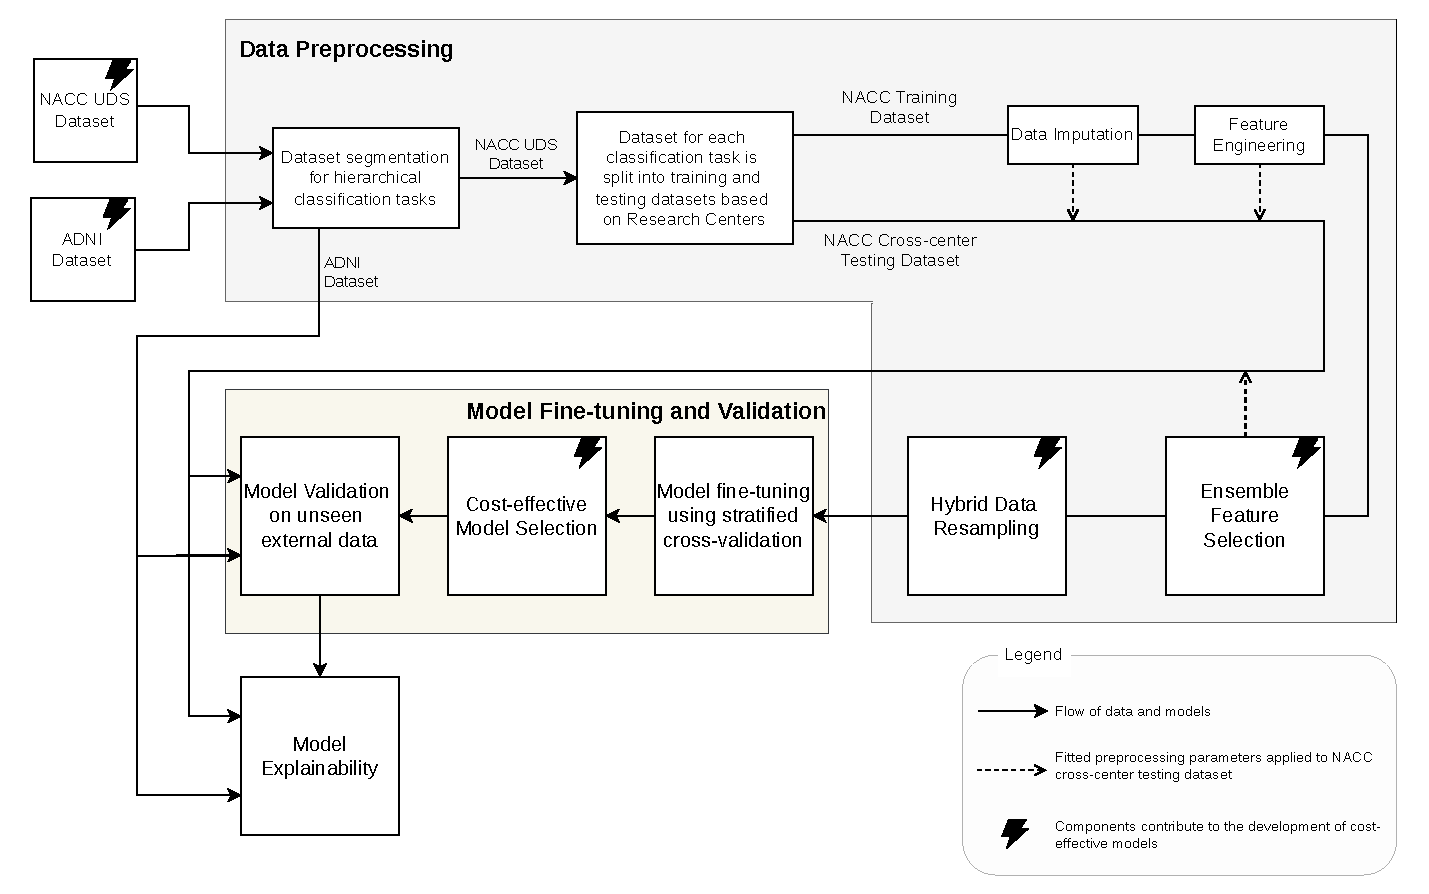
\includegraphics[width=\textwidth]{figures/research-framework.pdf}
    \caption{The research methodology framework diagram}
    \label{fig:research-method-diagram}
\end{figure}

Multiple machine learning algorithms were evaluated for predictive performance, computational efficiency, and interpretability. These models were trained in easily accessible features, such as demographics, health history, and basic assessment of behavior and cognitive functionality. The selected models were tested using external test data, specifically the Alzheimer’s Disease Neuroimaging Initiative (\acrshort{ADNI}) dataset, to assess their generalizability. A comprehensive assessment of the performance and calibration of the selected models were conducted. The methodology also incorporates Explainable Artificial Intelligence (\acrshort{XAI}) techniques to provide transparency in decision-making.

\hl{The development of cost-effective models is achieved through four main components in the proposed research methodology. The first component is the use of accessible data from both the NACC UDS and ADNI datasets. The second and third components are the ensemble feature selection and the hybrid data resampling, both of which reduce the feature subset and computational cost. The fourth component is the cost-effective model selection, which uses a novel algorithm to select faster and more efficient models while maintaining an acceptable performance.}

The research methodology was designed to handle the classification challenges of using accessible data, such as class imbalance and class overlap. It also promotes the development of cost-effective and generalizable models through optimized fine tuning and robust external validation. This research approach ensures clinical relevance and feasibility in real-world healthcare settings. In addition, the study methodology and results were reported according to the TRIPOD+AI guidelines \cite{Collins2024TRIPOD+AI}. The methods of this research are discussed in more detail in the sections of this chapter.

\section{Dataset Description}
The data in this study were obtained from two different datasets commonly used in the literature to implement robust model development and validation methods. The following subsections introduce the utilized datasets.

\subsection{National Alzheimer's Coordinating Center Uniform Data Set}
The main dataset used in this study is the Uniform Data Set (\acrshort{UDS}) provided by the National Alzheimer's Coordinating Center (\acrshort{NACC}) \cite{Beekly2007National}. The dataset is based on the UDS data freeze in March 2025. The dataset was collected through a longitudinal clinical evaluation of 44,713 subjects from 43 Alzheimer's disease research centers (\acrshort{ADRCs}) across the United States, starting from September 2005. Subjects have participated in annual visits by completing 16 forms related to multiple topics, including subject demographics, health history, neurological assessments, and diagnosis. Initial and follow-up visits have been made in person or through telephone calls. The total number of visits made by each subject ranged from one visit to 20 visits (mean = 3.85 and standard deviation = 3.15). The UDS forms have evolved into multiple versions since their inception in 2005. The utilization of the 2011 NIA-AA criteria for Alzheimer’s disease was among the updates during the major upgrade from version 2 to version 3 in 2015 \cite{Besser2018Version}. Some variables in UDS are only collected in some versions or were collected with different methods across versions. \hl{The complete list of the initially selected accessible variables extracted from the NACC UDS is provided in} Table~\ref{table:initial-uds-variables} in the appendix.

The NACC UDS is distinguished by its standardized longitudinal data collection, which captures information over multiple visits from large and diverse populations across multiple ADRCs in the United States. It is publicly available for research purposes and has been used in recent studies focused on developing predictive machine learning models \cite{abbas2024Explainable, Pang2023Predicting, Ren2023Improving}. It provides a wide range of easily accessible data, including demographic, health history, lifestyle factors, and cognitive assessments collected during routine medical examinations. This variety allows for comprehensive analysis and makes the dataset practical for clinical applications. Additionally, the NACC UDS encompasses a broad spectrum of cognitive status and various types of dementia, with diagnoses being recorded over time at multiple visits. This enables the development of models capable of predicting the risk of different types of dementia in the early stages. Moreover, data collected from ADRCs in different geographic regions with unique demographic, socioeconomic, and healthcare characteristics offers an opportunity to test the model’s ability to generalize across diverse clinical environments. These advantages collectively make the NACC UDS more practical for this study than other commonly used datasets. This decision supports the objectives of this study to develop generalizable and accessible models for the early prediction and intervention of cognitive impairment in clinical practice.

\hl{In addition to these advantages, the demographic composition of the NACC UDS cohort was examined. The subjects are mostly older adults, typically aged between about 60 and 80 years. The majority of subjects are female, and the level of education is relatively high, with a mean of around 15 years. The data are restricted to the United States, and some racial and ethnic groups are likely to be underrepresented. This pattern is commonly noted in dementia cohorts} \cite{Lennon2021Black, Nianogo2022Risk}. \hl{The NACC UDS is also a convenience sample of subjects attending Alzheimer's disease research centers, which explains the high prevalence of cognitive impairment in the data. This demographic skew has a direct impact on the generalizability of the models, since a model that learns from such data may not behave equally well when it meets populations of different demographic and socioeconomic backgrounds.}

\subsection{Alzheimer's Disease Neuroimaging Initiative Dataset}
The Alzheimer's Disease Neuroimaging Initiative (\acrshort{ADNI}) \cite{Weiner2024Overview} is a large-scale public-private partnership initiated in 2004 to define the progression of Alzheimer's disease (\acrshort{AD}). The study collects longitudinal data from healthy controls, individuals with mild cognitive impairment (\acrshort{MCI}), and AD patients. Data are gathered through a standardized battery of assessments at regular intervals, which includes accessible and low-cost features like demographics, medical history, and cognitive scale scores. The initiative has evolved through several phases (ADNI-1, ADNI-GO, ADNI-2, and ADNI-3), each expanding the study population. This dataset is a crucial resource for the external validation of the models to assess their generalizability across different studies.

The decision to use the ADNI dataset for external validation was made based on the research objectives. First, the ADNI initiative collects longitudinal data comprising the same categories of easily accessible features that were used in the models trained on the NACC UDS data. Second, the ADNI dataset is open access for researchers and has been widely used in dementia research. A similar study used the NACC UDS dataset for training and the ADNI dataset for external validation \cite{abbas2024Explainable}. More importantly, the ADNI dataset represents an independent study population collected under different protocols. Therefore, using it for testing provides a thorough assessment of the generalizability of the model, which is an important objective of this research. Validating against a standardized and external dataset is a crucial practice to confirm that a model's performance is reliable and not limited to the specific characteristics of the original training data.

\hl{The demographic composition of the ADNI data was also examined. Compared with the NACC UDS, the ADNI subjects show a similar pattern of older age, with a mean in the low seventies, and a comparably high level of education, with a mean of about 16 years. However, the ADNI cohort is more balanced in sex and even leans slightly towards male participants, unlike the female majority of the NACC UDS. Similar to the NACC UDS, the majority of the ADNI participants are volunteers based in the United States} \cite{Weiner2024Overview}. \hl{This limited representativeness should be taken into account when the generalizability of the externally validated models is interpreted.}

\section{Hierarchical Classification Tasks}
One of the objectives of this study is to develop cost-effective machine learning models for the early prediction of CI. To achieve this objective, it is crucial to identify the current and future cognitive status as normal, cognitively impaired, or dementia. Identifying the current and future status of the subjects' cognitive ability allows for timely and precise intervention plans. It appears that this is a complex classification problem that includes classifying CI at two different time points and across three different overlapping and imbalanced cognitive stages. Using easily accessible data adds another layer of complication to the classification problem, as it makes it difficult for the classification models to differentiate multiple classes in such complex data domains. 

To simplify the classification problem, the main problem was segmented into five smaller binary classification tasks using a hierarchical classification strategy. A visual explanation of this segmentation is provided in Figure~\ref{fig:classification-tasks}. This figure illustrates how the problem was broken down using two main dimensions. The first dimension is the timeline, which separates tasks into current cognitive status classification and future cognitive status prediction. The second dimension is the diagnosis. This dimension distinguishes between general diagnoses (like normal cognition (\acrshort{NC}) vs. CI) and specific diagnoses (like cognitive impairment but not demented (\acrshort{CIND}) vs. dementia or classifying the etiology as AD vs. non-AD). Furthermore, the arrows in the diagram represent common diagnosis paths followed in clinical practice. This shows that this segmentation method aligns with clinical utility.

\begin{figure}[ht]
    \centering
    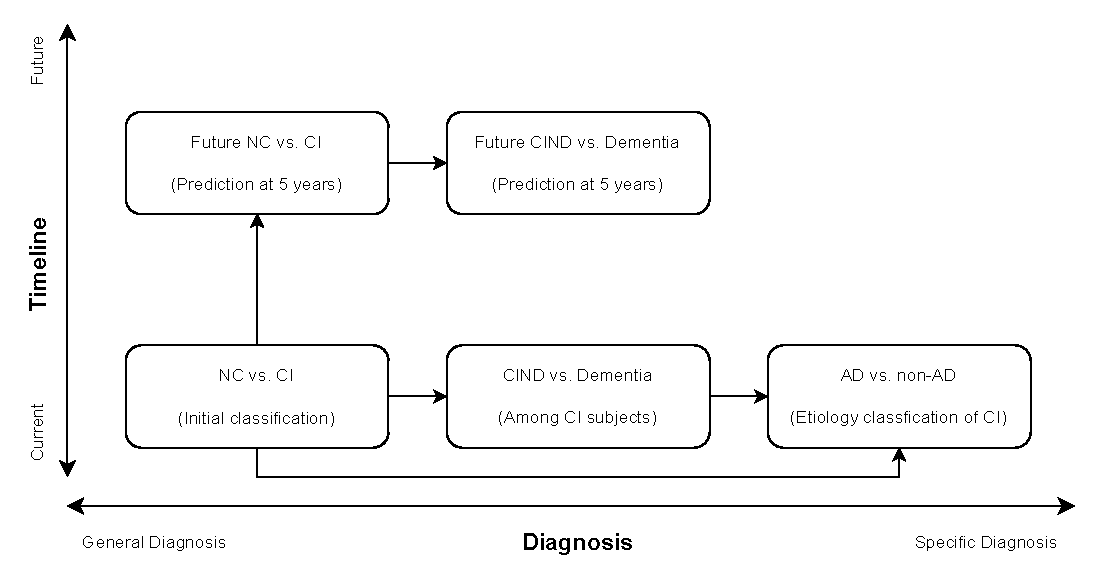
\includegraphics[width=\textwidth]{figures/classification-tasks.pdf}
    \caption[The segmentation of the classification problem into five tasks using hierarchical classification strategy]{The segmentation of the classification problem into five tasks using a hierarchical classification strategy\hl{, organised along two dimensions: the timeline (current versus future) and the diagnosis (general versus specific), and connected by arrows that represent common diagnosis paths in clinical practice}}
    \label{fig:classification-tasks}
\end{figure}

For the current cognitive status classification, both input features and target labels were derived from the ' baseline visit of the subjects. The classification task was then divided into two hierarchical tasks. First, a model was trained to differentiate NC subjects from all CI subjects. Second, another model was trained only on impaired subjects to further classify them as CIND or dementia. \hl{Demographic comparisons of the three cognitive statuses are summarized in} Table~\ref{table:ci-classification-demographics} \hl{for NACC UDS dataset and} Table~\ref{table:adni-classification-demographics} \hl{for ADNI dataset.}

\begin{table}[htbp]
\centering
\caption{Demographic characteristics of the NACC UDS subjects used in the current cognitive status classification tasks}
\label{table:ci-classification-demographics}
\footnotesize
\begin{tabular}{lcccc}
\toprule
 & \multicolumn{4}{c}{Cognitive Status} \\
\cmidrule{2-5}
Characteristic & NC & CIND & Dementia & Total \\
 & (n=21,919) & (n=14,445) & (n=17,151) & (N=53,515) \\
\midrule
\textbf{Age, years} \\
\quad Mean ± \acrshort{SD} & 69.4 ± 10.8 & 71.9 ± 9.4 & 72.3 ± 10.4 & 71.0 ± 10.4 \\
\\
\textbf{Sex} \\
\quad Female & 14,361 (65.5\%) & 7,468 (51.7\%) & 8,879 (51.8\%) & 30,708 (57.4\%) \\
\quad Male & 7,558 (34.5\%) & 6,977 (48.3\%) & 8,272 (48.2\%) & 22,807 (42.6\%) \\
\\
\textbf{Education, years} \\
\quad Mean ± SD & 15.8 ± 3.0 & 15.2 ± 3.4 & 14.5 ± 3.7 & 15.2 ± 3.4 \\
\\
\textbf{Marital Status} \\
\quad Married & 12,819 (58.5\%) & 9,050 (62.7\%) & 11,877 (69.2\%) & 33,746 (63.1\%) \\
\quad Other & 9,100 (41.5\%) & 5,395 (37.3\%) & 5,274 (30.8\%) & 19,769 (36.9\%) \\
\bottomrule
\end{tabular}
\end{table}

\begin{table}[htbp]
\centering
\caption{Demographic characteristics of the ADNI subjects used in the current cognitive status classification task}
\label{table:adni-classification-demographics}
\footnotesize
\begin{tabular}{lcccc}
\toprule
 & \multicolumn{4}{c}{Cognitive Status} \\
\cmidrule{2-5}
Characteristic & NC & CIND & Dementia & Total \\
 & (n=514) & (n=832) & (n=429) & (N=1,775) \\
\midrule
\textbf{Age, years} \\
\quad Mean ± \acrshort{SD} & 73.4 ± 6.4 & 73.3 ± 7.5 & 74.5 ± 7.5 & 73.6 ± 7.2 \\
\\
\textbf{Sex} \\
\quad Female & 274 (53.3\%) & 327 (39.3\%) & 184 (42.9\%) & 785 (44.2\%) \\
\quad Male & 240 (46.7\%) & 505 (60.7\%) & 245 (57.1\%) & 990 (55.8\%) \\
\\
\textbf{Education, years} \\
\quad Mean ± SD & 16.4 ± 2.6 & 16.1 ± 2.8 & 15.4 ± 2.9 & 16.0 ± 2.8 \\
\\
\textbf{Marital Status} \\
\quad Married & 335 (65.2\%) & 633 (76.1\%) & 360 (83.9\%) & 1,328 (74.8\%) \\
\quad Other & 179 (34.8\%) & 199 (23.9\%) & 69 (16.1\%) & 447 (25.2\%) \\
\bottomrule
\end{tabular}
\end{table}

The same hierarchical structure was designed for the early prediction of future cognitive status. However, specific criteria were applied for the inclusion of subjects for these prediction tasks. Only subjects with a baseline visit and a follow-up visit five years later were included. The input data for these tasks were extracted from the baseline visits, whereas the target classes were based on the diagnosis at a follow-up visit made approximately five years later. To accommodate for variability in visit timelines, a time frame of six months before or after the five-year mark was used. Subjects whose follow-up visits did not occur within this time frame were excluded. This future prediction task was also divided into two binary tasks: one for predicting future NC versus future CI status, and a second to differentiate future CIND from future dementia. Table~\ref{table:ci-prediction-demographics} and Table~\ref{table:adni-prediction-demographics} \hl{summarize the demographic characteristics of the subjects included in the future cognitive status prediction tasks for the NACC UDS and ADNI datasets, respectively.}

\begin{table}[htbp]
\centering
\caption{Demographic characteristics of the NACC UDS subjects used in the five years cognitive status prediction tasks}
\label{table:ci-prediction-demographics}
\footnotesize
\begin{tabular}{lcccc}
\toprule
 & \multicolumn{4}{c}{Cognitive Status} \\
\cmidrule{2-5}
Characteristic & NC & CIND & Dementia & Total \\
 & (n=6,612) & (n=2,334) & (n=3,399) & (N=12,345) \\
\midrule
\textbf{Age, years} \\
\quad Mean ± SD & 70.2 ± 9.2 & 72.9 ± 9.2 & 72.6 ± 9.6 & 71.4 ± 9.4 \\
\\
\textbf{Sex} \\
\quad Female & 4,354 (65.8\%) & 1,208 (51.8\%) & 1,715 (50.5\%) & 7,277 (58.9\%) \\
\quad Male & 2,258 (34.2\%) & 1,126 (48.2\%) & 1,684 (49.5\%) & 5,068 (41.1\%) \\
\\
\textbf{Education, years} \\
\quad Mean ± SD & 16.1 ± 2.8 & 15.6 ± 3.2 & 15.2 ± 3.5 & 15.8 ± 3.1 \\
\\
\textbf{Marital Status} \\
\quad Married & 3,918 (59.3\%) & 1,426 (61.1\%) & 2,522 (74.2\%) & 7,866 (63.7\%) \\
\quad Other & 2,694 (40.7\%) & 908 (38.9\%) & 877 (25.8\%) & 4,479 (36.3\%) \\
\bottomrule
\end{tabular}
\end{table}

\begin{table}[htbp]
\centering
\caption{Demographic characteristics of the ADNI subjects used in the five years cognitive status prediction task}
\label{table:adni-prediction-demographics}
\footnotesize
\begin{tabular}{lcccc}
\toprule
 & \multicolumn{4}{c}{Cognitive Status} \\
\cmidrule{2-5}
Characteristic & NC & CIND & Dementia & Total \\
 & (n=348) & (n=309) & (n=169) & (N=826) \\
\midrule
\textbf{Age, years} \\
\quad Mean ± \acrshort{SD} & 72.2 ± 6.5 & 72.3 ± 7.2 & 73.4 ± 6.4 & 72.4 ± 6.8 \\
\\
\textbf{Sex} \\
\quad Female & 190 (54.6\%) & 117 (37.9\%) & 72 (42.6\%) & 379 (45.9\%) \\
\quad Male & 158 (45.4\%) & 192 (62.1\%) & 97 (57.4\%) & 447 (54.1\%) \\
\\
\textbf{Education, years} \\
\quad Mean ± SD & 16.7 ± 2.5 & 16.1 ± 2.7 & 15.9 ± 2.8 & 16.3 ± 2.7 \\
\\
\textbf{Marital Status} \\
\quad Married & 233 (67.0\%) & 230 (74.4\%) & 137 (81.1\%) & 600 (72.6\%) \\
\quad Other & 115 (33.0\%) & 79 (25.6\%) & 32 (18.9\%) & 226 (27.4\%) \\
\bottomrule
\end{tabular}
\end{table}

\newpage
The data selection method for future cognitive status prediction tasks is illustrated in Figure~\ref{fig:prediction-data-selection}. Each row in the diagram represents visits made by a single subject. Subject's visits are donated with boxes. A selection window was set between 54 and 66 months (4.5 to 5.5 years) from the baseline visit (initial visit). Subjects who made a visit within the selection window were selected (denoted with a tick symbol). Subjects were excluded if they did not make a visit within the selection window (denoted with a cross sign). For selected subjects, data from the baseline visit are used as input data (boxes with ``IN''), and target classes are obtained from the visits made within the selection window (boxes with ``T''). It can be noticed that the selection of the subjects depends solely on the availability of visits made within the selection window, regardless of the number of visits made and the regularity of the time interval between visits. 

\begin{figure}[ht]
    \centering
    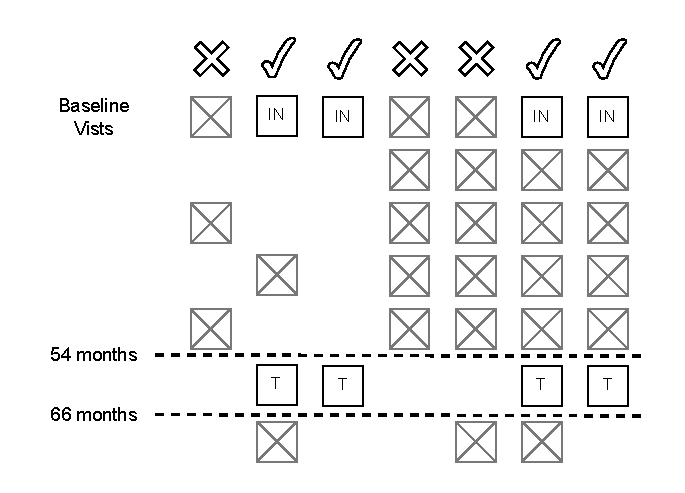
\includegraphics[width=0.8\linewidth]{figures/prediction-data-selection.pdf}
    \caption[The data selection method for the prediction of future cognitive status]{The data selection method for the prediction of future cognitive status\hl{, based on a 4.5--5.5 year selection window from the baseline visit. A tick symbol indicates included subjects, while a cross symbol indicates excluded subjects. Box labels ``IN'' and ``T'' denote input data and target classes, respectively.}}
    \label{fig:prediction-data-selection}
\end{figure}

It should be noted that cognitive status in the NACC UDS is classified as normal cognition, MCI, impaired-not-MCI, or dementia. Impaired-not-MCI refers to subjects who show cognitive difficulties but do not satisfy the clinical criteria for MCI. In this research work, MCI and impaired-not-MCI have been combined into a single class that represents CIND. Impaired-not-MCI cases are not treated as normal because they could indicate a risk of future progression to severe cognitive impairment. On the other hand, having impaired-not-MCI as a separate class could increase the complexity of the classification problem. This approach aligns with the objectives of this study to develop cost-effective early prediction models of CI. Compared to the literature, most of the studies that use NACC UDS do not clearly state how they address impaired-not-MCI cases \cite{abbas2024Explainable, Pang2023Predicting, Ren2023Improving}. These studies classify cognitive status as NC, MCI, and dementia. 

In addition to the cognitive status classification, another classification task is implemented to classify the subtype of current CI. The model in this task classifies the etiology of CI as AD versus other non-AD etiologies. The input data and the target classes are obtained from baseline visits of subjects with CIND or dementia. Subjects with normal cognition are not included in this classification task. Demographic differences between AD subjects and non-AD subjects are summarized in Table~\ref{table:ci-type-demographics}.

\begin{table}[htbp]
\centering
\caption{Demographic characteristics of the NACC UDS subjects used in the cognitive impairment subtype classification task}
\label{table:ci-type-demographics}
\footnotesize
\begin{tabular}{lcccc}
\toprule
 & \multicolumn{3}{c}{Cognitive Impairment Type} & \\
\cmidrule{2-4}
Characteristic & AD & Non AD & Total \\
 & (n=18,201) & (n=13,441) & (N=31,642) \\
\midrule
\textbf{Age, years} \\
\quad Mean ± SD & 73.7 ± 9.6 & 70.0 ± 10.1 & 72.1 ± 10.0 \\
\\
\textbf{Sex} \\
\quad Female & 9,923 (54.5\%) & 6,448 (48.0\%) & 16,371 (51.7\%) \\
\quad Male & 8,278 (45.5\%) & 6,993 (52.0\%) & 15,271 (48.3\%) \\
\\
\textbf{Education, years} \\
\quad Mean ± SD & 14.7 ± 3.7 & 14.9 ± 3.5 & 14.8 ± 3.6 \\
\\
\textbf{Marital Status} \\
\quad Married & 12,162 (66.8\%) & 8,794 (65.4\%) & 20,956 (66.2\%) \\
\quad Other & 6,039 (33.2\%) & 4,647 (34.6\%) & 10,686 (33.8\%) \\
\bottomrule
\end{tabular}
\end{table}

The use of hierarchical binary classification has proven to produce a better classification accuracy compared to the multi-classification approach in studies related to dementia \cite{Ren2023Improving}. The complexity of the data that a single classifier needs to learn for multi-classification has been reduced by decomposing the data to simpler data domains. Furthermore, in imbalanced and overlapped domains, separating classes promotes focused feature selection, targeted data resampling, and tailored model tuning to improve classification performance. Additionally, this approach increases the clinical utility of classification models. Implementing staged classification mirrors the real-world diagnostic flow in which impairment is first diagnosed (normal vs. impaired) before the severity of impairment is identified. It also allows for the use of specialized models for specific use cases. Moreover, hierarchical binary classification supports the transparent and clinically meaningful interpretability of the model through an independent explanation of each decision stage.

In contrast, hierarchical binary classification has pitfalls that could affect the accuracy and interpretation of the outputs of multiple models. Classification at multiple levels could result in compound errors where misclassifications at the first level could impact the correctness of the downstream binary model. Additionally, combining the interpretation of the output of multiple models is necessary to gain an overall understanding of the subject's cognitive status. Not to mention the added workload and complexity in training, tuning, and evaluating multiple models. With these concerns in mind, the research methodology of this study was designed around the hierarchical binary classification approach because of its potential to improve classification performance and clinical practicality.

\section{Data Preprocessing}
Data preprocessing improves the quality of the data by cleaning, transforming, and organizing the raw data to be suitable for analysis. It is undeniably the most critical process for developing an accurate classification model. The quality of the data has a direct impact on the model performance, especially on imbalanced and overlapped data domains. As a result, significant effort and emphasis were dedicated to this phase of the research work. The primary objective of data preprocessing is to improve data quality and mitigate the impact of data irregularities, such as class imbalance and overlap. Class overlap measures were used to guide data preprocessing techniques and assess their effectiveness. In this research, data preprocessing can be categorized into data imputation, feature engineering, feature selection, and data resampling.

The initial raw data were extracted from the NACC UDS and ADNI datasets based on easily accessible data. According to the categorization by affiliated neurologists and neuropsychologists \cite{Ren2023Improving}, easily accessible data can be acquired quickly and efficiently without the need for specialized tools or advanced skills. A general practitioner can collect these data during primary care visits by conducting direct interviews with the subjects or their caregivers. These data include the subject's demographics, health and family history, behavioral surveys, and basic functional and cognitive tests. All of these data were classified as lower cost in a three-tiered categorization based on the cost required to obtain the associated information \cite{Ren2023Improving}. Refer to Table \ref{table:initial-uds-variables} in the appendix for more details of the initially selected accessible data variables.

\subsection{Data Imputation}
It is important to properly handle missing data to ensure model reliability and to prevent biases that may result from incomplete observations. In this study, data imputation was only applied to the NACC UDS dataset. Samples with missing values in the ADNI dataset were excluded to maintain the integrity of external testing and to avoid introducing differing imputation assumptions across datasets. Most of the missing data in the NACC UDS came from the nature of collecting data from multiple centers and utilizing different versions of data collection forms. Subjects or their informants were sometimes unable or unwilling to answer certain questions during the interview. Additionally, systematic missing data occurred due to skip patterns in the assessment protocol that prevented follow-up questions. It has been noticed that variables related to physical measurement, such as height and weight, comprise the highest percentage of missing data. This could be due to challenges in performing the assessment during telephone visits. The percentages of missing data in different NACC UDS forms for the data of all classification tasks are presented in Table \ref{table:miss-data} in the appendix.

The data imputation workflow consists of multiple steps. First, any data sample with 50\% or more missing values was removed. This limits the risk of excessive information loss against the potential distortion introduced by imputing very sparse samples. This method is applied and verified by other studies in the literature \cite{abbas2024Explainable, Vyas2022Identifying}. Second, the remaining missing values were imputed using appropriate statistical methods based on the type of variables. The mode is used for nominal variables, the median for ordinal variables, and the mean for continuous data. Refer to Table \ref{table:initial-uds-variables} in the appendix for the types of variables. The missing values of the derived variables, such as the total Geriatric Depression Scale score (NACCGDS) and the body mass index (NACCBMI), were recalculated using the imputed values of the source variables. Statistical imputation techniques were employed because the rate of missing values is small in addition to their simplicity, computational efficiency, and ability to maintain the central tendency of the dataset. This imputation method is commonly used by other studies that use the same dataset \cite{abbas2024Explainable, Wang2018Predictive}. To prevent data leakage, imputation parameters (the mode, median, and mean) were first fitted using only the training dataset and then applied to the missing data in the testing dataset. Finally, the values of the Functional Activities Questionnaire (\acrshort{FAQ}) required special attention. The “never did” category was retained as a valid value if it represented at least 3\% of observations. Treating "never did" as a valid value preserves meaningful differences in functional ability and enhances the integrity of the analysis. For instance, since many people have not filed taxes before, preserving a specific category better reflects their functional ability. These procedures were essential to maintain the quality of the data and support reliable downstream modeling in this research work.

\subsection{Feature Engineering}
Effective feature engineering is required to convert raw clinical data into informative input that improves the efficiency of the modeling process and enhances the performance of the model. Guided by statistical criteria and domain knowledge from the literature, systematic transformations were applied to categorical and continuous features.

The feature engineering process involved the alignment of data from the NACC UDS and ADNI datasets. Various categorical variables were found to be defined using different sets of categories across the two datasets. Therefore, an alignment of these categories was performed. For instance, the primary language variable in the NACC UDS dataset has been transformed to align with the categories in the ADNI dataset (English, Spanish, and others). This is done by aggregating other languages into one category. Other transformed demographic features include marital status and type of residence. Variables related to the subject's health history were converted to binary features by grouping inactive and active categories to indicate the presence of the condition. This binarization was required due to the low representation of these values and to align the NACC UDS dataset with the ADNI dataset. This alignment was a critical requirement to ensure data consistency, which was required for the external validation phase. \hl{Previous studies used similar alignment steps that successfully aligned the feature in the NACC UDS and ADNI datasets} \cite{abbas2024Explainable, Qiu2022Multimodal}. Additionally, as part of feature engineering, categorical features with a dominant category accounting for 97\% of the samples were excluded to prevent potential model bias and improve performance. Furthermore, some initially selected variables from the NACC UDS dataset were excluded because they are not available in the ADNI dataset. The excluded variables are listed in Table~\ref{table:excluded-dominant-features} in the appendix. \hl{These feature engineering choices were guided by statistical criteria and prior literature to minimize potential bias, although it is acknowledged that the alignment and binarization steps may cause a minor loss of information.}

In this research, the relationship between the features was calculated and examined. Since the dataset consists of a mixture of continuous and categorical features, suitable correlation methods were used depending on the type of the features. Cramer's V was used to calculate the correlation between categorical features and Pearson was utilized to measure correlation between the continuous features. Additionally, the correlation ratio for multiple categorical and continuous feature pairs was calculated. An absolute correlation ratio above 0.70 was considered high and was addressed by merging the correlated features or excluding the less informative features. Features with moderate correlations were managed during the subsequent feature selection.

Finally, proper encoding and scaling methods were used to maintain the integrity of the original data while preparing the data for modeling. Categorical variables were encoded according to their characteristic. One-hot encoding was applied to nominal features, whereas ordinal features were encoded using ordinal encoding to preserve the order of categories. Continuous variables were scaled with a robust scaler to reduce the impact of outliers. \hl{To prevent data leakage, the encoding and scaling parameters were fitted on the training dataset only and then applied to the testing dataset.}
% TODO: (optional) draw figure that show how features flow from initial set, to ADNI available selection, to feature selection (refer to 41598_2024_51985_MOESM1_ESM.pdf)

In the next sections, feature selection and data resampling to handle class imbalance and overlap are discussed. The implementation of these two important steps of data preprocessing was guided by the characteristics of class overlap. The following section provides a detailed discussion on the problem of class overlap.

\subsection{Class Overlap} \label{class-overlap-section}
Class overlap is a significant issue that occurs when examples from different classes are located in the same region of the data. This makes it harder for models to set clear decision boundaries. The problem is exacerbated in imbalanced domains, where the scarce minority class examples may primarily reside in regions shared with the majority class, making their classification significantly more difficult. In overlapped and imbalanced domains, addressing class imbalance is often insufficient without handling class overlap. Classification performance is significantly affected by the presence of class overlap even with balanced datasets \cite{Pattaramon2021On}

There are several factors that can lead to class overlap \cite{Santos2022Joint}. An important reason is inherent ambiguity, which means that some classes are very similar and difficult to differentiate. Another factor is the limited feature representation, which means that the measured features do not pick up enough of the differences between classes. Additionally, diagnosis mistakes or labeling errors can cause overlapping instances and create complex class boundaries. All of these factors could apply to the datasets used in this study.

Class overlap appears in various forms and can be attributed to different underlying causes and characteristics of the data \cite{Santos2023Unifying}. Therefore, it is regarded as a heterogeneous concept. Identifying class overlap is crucial because it allows for a more detailed understanding of the problem. Different types of overlap may require different approaches to mitigate. Additionally, a comprehensive view of class overlap enables researchers to develop more targeted and effective solutions \cite{Santos2023Unifying}. The identification of class overlap is done using various methods that aim to characterize and quantify the ambiguous regions. These identification methods often lead to different representations of class overlap. Each representation highlights a particular aspect of the phenomenon. Common representations include:
\begin{itemize}
\item \textbf{Feature Overlap}: This refers to the overlap in the distribution of individual features between classes.
\item \textbf{Instance-Level Overlap}: This focuses on specific data points that lie in ambiguous regions, often referred to as "borderline" or "noisy" instances. It is based on characteristics of local data (local information).
\item \textbf{Structural Overlap}: This considers the overlap in the underlying data structure or clusters. It is based on geometrical and graph-based properties of the data. This may indicate that class clusters are not well separated in the data space.
\end{itemize}
\vspace{2em}

% It is important to note that merely measuring the class overlap degree (a single numerical value indicating the extent of overlap) is often not sufficient \cite{Santos2022Joint}. This is because a single degree measure might miss the specific nature or cause of the overlap. For instance, two datasets might have the same degree of overlap but suffer from entirely different types of overlap (e.g., one due to inherent ambiguity, another due to noisy labels). A single metric is not capable of capturing the heterogeneity of the problem or providing insights about the class overlap, such as which features or instances are impacted. Therefore, understanding the different representations and causes of overlap is essential for effective analysis and resolution.

There are available measures that are used to quantify class overlap \cite{Santos2022Joint}. Each measure offers different insights into the type of overlap. It is necessary to use different class overlap measures to build a thorough understanding of how classes interact. The measures listed below were employed in this study to obtain information about the class overlap. These insights were used to design optimized techniques, such as feature selection and data resampling. These class overlap measures cover various representations of the overlapped domains, including feature overlap, instance-level overlap, and structural overlap.

\begin{itemize}
\item \textbf{Maximum Fisher's Discriminant Ratio (\acrshort{F1})}: This is a feature overlap measure. It is used to define the discriminative power of individual features \cite{Lorena2019How}. For its mechanism, Fisher's discriminant ratio, which is based on class means and variances, is computed for each feature. The maximum value found among all the features is then used. Typically, the inverse of this value is taken, where higher values indicate more overlap.

\item \textbf{Borderline Examples}: This measure is associated with the overlap of instances. It quantifies the percentage of data points that are located near the decision boundary between classes. Data examples are categorized according to their local neighborhood (e.g., $k=5$). An example is designated as "borderline" if a specific number of its neighbors, such as two or three, belong to the opposite class. The final measure is the total count of these examples normalized by the size of the dataset.
\item \textbf{k-Disagreeing Neighbors (\acrshort{kDN})}: This measure is used to measure the local overlap for an individual instance (instance-level overlap) \cite{Smith2013Instance}. For each instance, the percentage of k-nearest neighbors that do not belong to the same class as the instance is calculated. The value is used to indicate whether the data point is in a safe or overlapped region. This can be averaged over all samples to produce a global measure.
\item \textbf{Fraction of Borderline Points (\acrshort{N1})}: This measures structural overlap by assessing the complexity of the decision boundary \cite{Ho2002Complexity}. It indicates how deeply the classes are intertwined. For its mechanism, a minimum spanning tree (\acrshort{MST}) is constructed for the entire dataset. The measure is the proportion of examples in the dataset that are connected by an edge in the MST to an example from the opposite class.
\end{itemize}
\vspace{2em}

These class overlap measures are discussed in more detail in a recent review \cite{Santos2022Joint}. The following sections explain how insights from these class overlap measures were used to guide the feature selection and data resampling methods in this study.

\subsection{Ensemble Feature Selection}
In the context of developing cost-effective and accessible predictive models for CI, feature selection constitutes a critical step in the development of robust and generalizable machine learning models. Selecting the most informative subset from a larger pool of features is essential to mitigate high dimensionality, reduce the risk of overfitting, and improve model interpretability and computational efficiency. All of these advantages are aligned with the objectives of this study. \hl{In particular, reducing the feature subset is one of the main components that promote the cost-effectiveness of the developed models, since fewer features lower the data collection and computational costs.} The feature selection method in this study was designed based on a two-step automated approach. The strategy combines an ensemble of diverse feature ranking methods with a class overlap-driven thresholding technique. These two steps are explained in the following subsections. Refer to Figure~\ref{fig:feature-selection} for an overview of the proposed feature selection method.

\begin{figure}
    \centering
    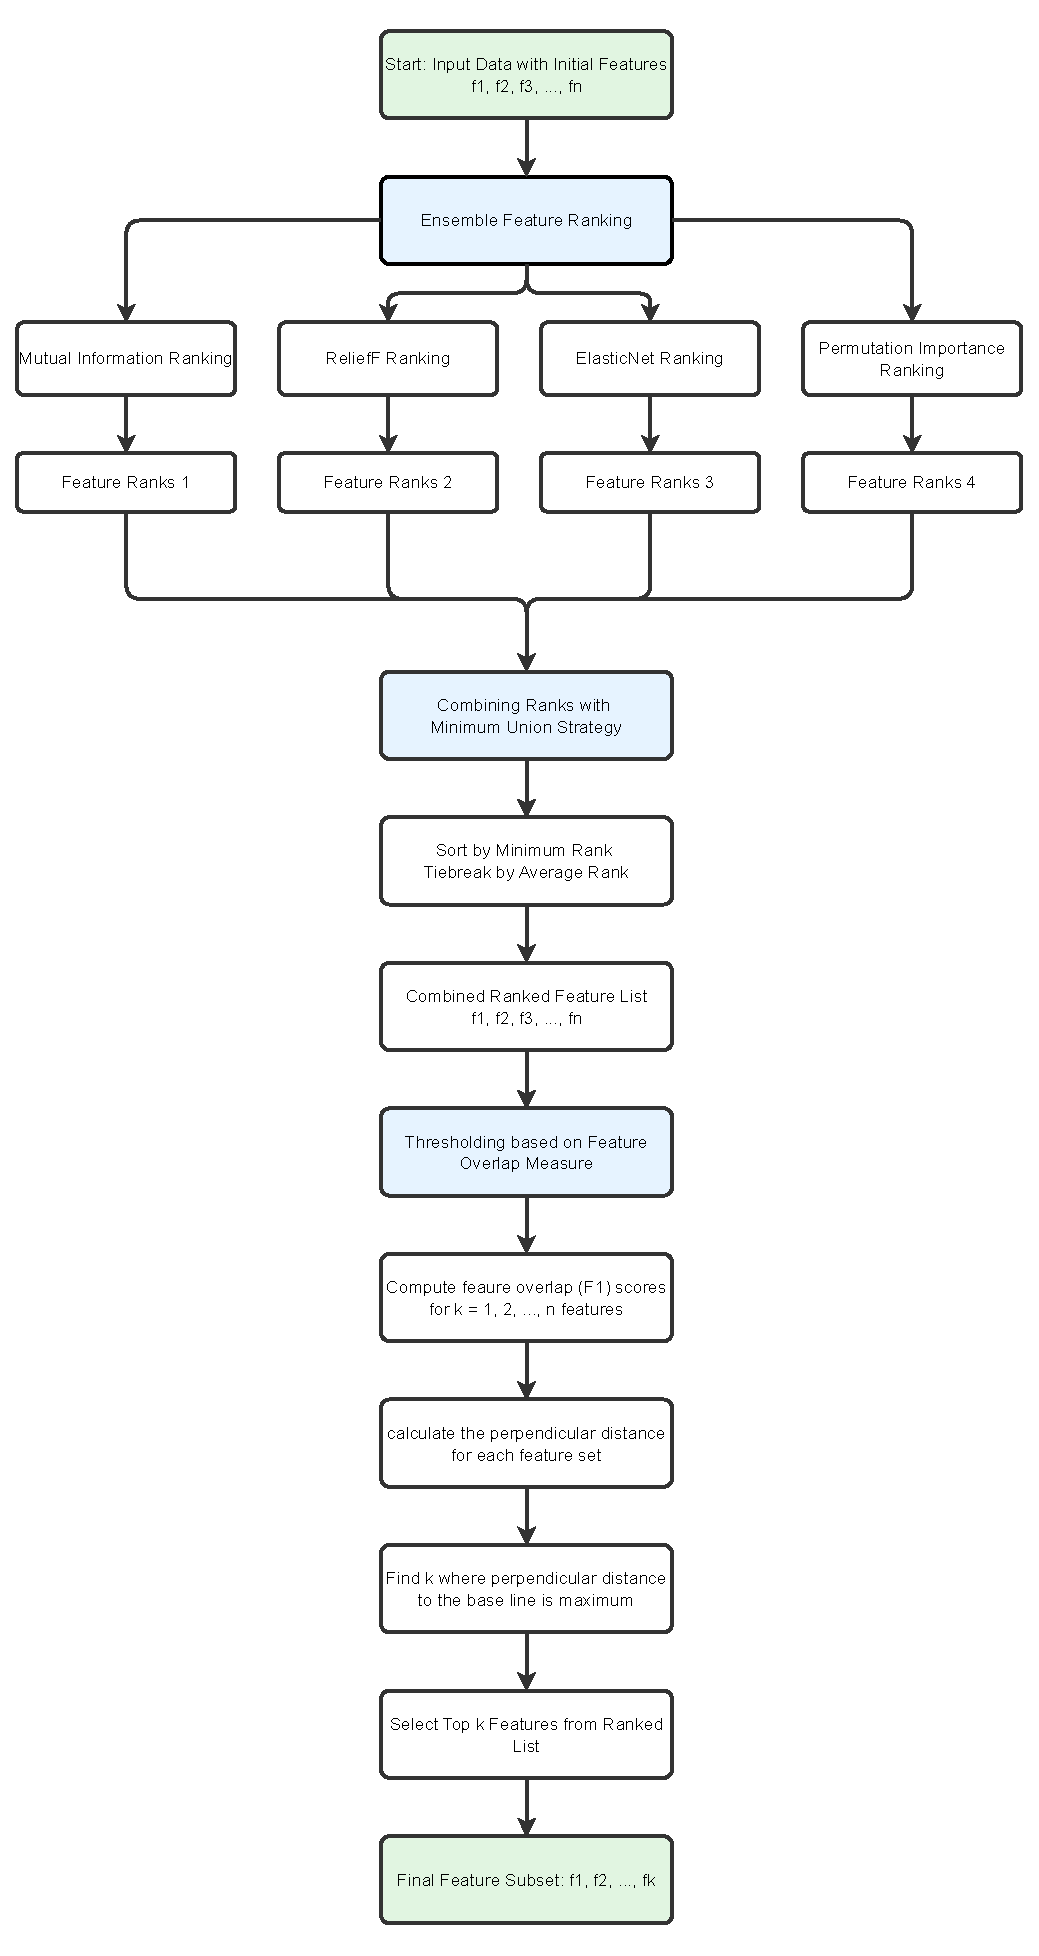
\includegraphics[width=0.7\textwidth]{figures/feature-selection-method.pdf}
    \caption[Flowchart of the proposed ensemble feature selection method]{Flowchart of the proposed ensemble feature selection method\hl{. It combines multiple feature ranking methods and a class overlap-driven thresholding technique to select the most informative features}}
    \label{fig:feature-selection}
\end{figure}

\subsubsection{Combination Step: Aggregating Feature Rankings}
The objective of this step is to combine the feature rankings obtained from various feature selection methods into a single ranking. Four feature selection methods have been utilized: mutual information \cite{Peng2005Feature}, ReliefF \cite{Robnik-ikonja2003Theoretical}, elastic net \cite{Zou2005Regularization}, and permutation importance using random forest. Each of these methods follows a different approach to select informative features, including filter, wrapper, and embedded techniques. These approaches have different sensitivities to data characteristics such as noise, feature correlation, and non-linear interactions. As an example, Mutual Information and ReliefF are effective at detecting non-linear relationships, whereas elastic net is effective at feature correlation. Therefore, the use of this diverse ensemble approach ensures a comprehensive evaluation of feature importance from multiple analytical perspectives. The results of the feature ranking methods were analyzed using Spearman correlation to ensure that these feature selection methods are complementary and do not highly overlap.
% TODO: table #t comparing the feature selection methods

The minimum union method was utilized to combine these individual rankings into a unified list. The features were added to the unified list based on their minimum rank across all four methods. The average of the ranks of a feature across the four methods was used in cases where multiple features have the same minimum rank. This method resulted in a strong and stable sorted list of features, which was used by the following step to identify the optimal subset of features. Figure~\ref{fig:minimum-union} illustrates the proposed feature ranking method. 

\hl{The ensemble feature ranking approach is adopted to avoid biased or unstable results that can be obtained by using a single feature ranking method, particularly in high-dimensional clinical and neuropsychological data. This approach has been successfully employed across predictive modeling studies in the literature. For example, \mbox{\cite{Pereira2018Neuropsychological}} combined multiple filter and embedded methods to predict the conversion from MCI to AD. It was found that combining subsets from different selection methods creates a consensus that improves the robustness, stability, and generalizability of the selected features. Furthermore, this finding was confirmed by another study } \cite{Spooner2023Ensemble} \hl{that applied ensemble feature selection with data-driven thresholding on Alzheimer's disease datasets, including the ADNI cohort.}

\begin{figure}[ht]
    \centering
    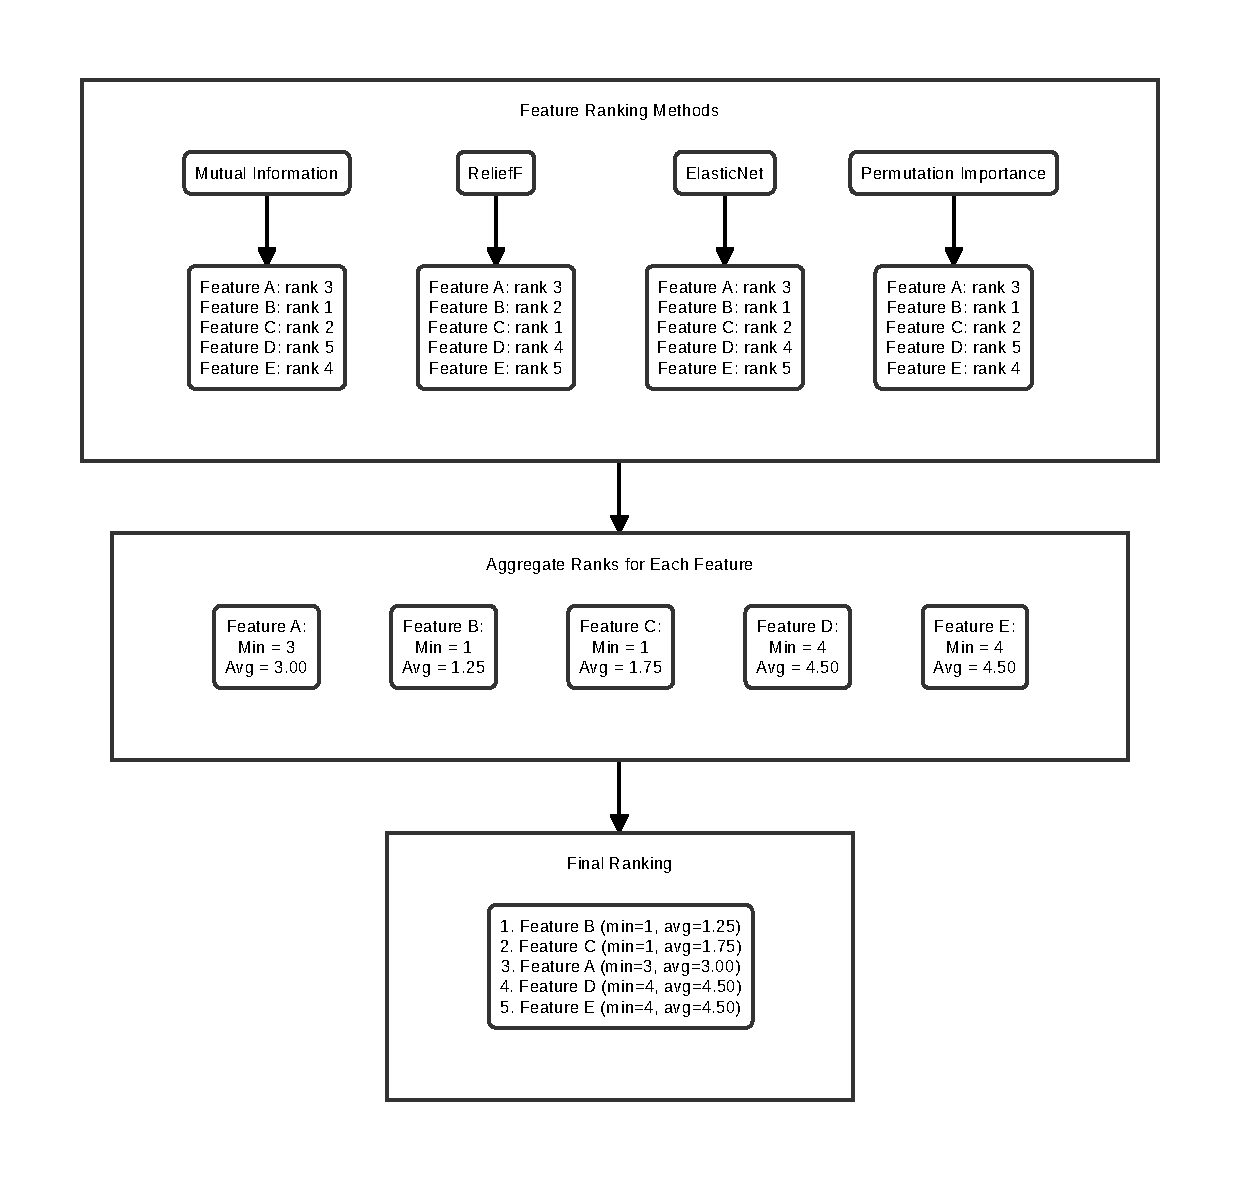
\includegraphics[width=\textwidth]{figures/minimum_union_diagram.pdf}
    \caption[Illustration of the minimum union feature ranking aggregation method]{Illustration of the minimum union feature ranking aggregation method\hl{. The method merges four separate feature rankings into one unified ranking by their minimum rank}}
    \label{fig:minimum-union}
\end{figure}

\subsubsection{Thresholding Step: Selecting Features Based on Class Overlap Measures}
The second step addresses the challenge of determining the optimal number of features, denoted as \textit{k}, to be retained from the ranked features. To do this, a class overlap measure is used as a dynamic thresholding mechanism, instead of random feature counts or levels of statistical significance. Using the class overlap measure as a threshold selects the optimal set of features that minimizes the inherent complexity of the data. As a result, it facilitates more effective model training and improves predictive performance.

The process begins by iteratively constructing subsets of features, starting with the top-ranked feature and progressively adding one feature at a time from the ranked list of features from the previous combination step. For each subset of \textit{k} features, the class overlap was quantified using a modified F1 measure of all features in the subset. The F1 measure was computed by first calculating the Fisher's discriminant ratio for each feature in the subset. This calculation is presented in equation \eqref{eq:fisher-ratio}. After that, the inverse of the summation of these values was obtained, as shown in equation \eqref{eq:f1-measure-feature-set}. This inverse ensures that feature subsets with better overall discriminative power (higher individual discriminant ratios) result in smaller F1 values. On the other hand, subsets with poorer class separability produce larger F1 values. Consequently, during feature selection, the objective was to minimize the F1 value to identify the set of features that provides the most effective class discrimination.

\newpage

\begin{equation}
    F1_i = \frac{\sum_c p(c) \times (\mu_c - \mu)^2}{\sum_c p(c) \times \sigma_c^2}
    \label{eq:fisher-ratio}
\end{equation}
Where:
\begin{itemize}
    \item $p(c)$ = proportion of samples in class $c$
    \item $\mu_c$ = mean value of feature $x_i$ for class $c$
    \item $\mu$ = overall mean of feature $x_i$ across all samples
    \item $\sigma_c^2$ = variance of feature $x_i$ within class $c$
\end{itemize}
\vspace{2em}

The Fisher's discriminant ratio of a single feature ($F1_i$) is calculated by computing the ratio of between-class scatter (numerator) to within-class scatter (denominator). Features that exhibit larger between-class separation relative to their within-class variance yield higher discriminant ratios. This indicates that the feature has better class separability.

\begin{equation}
    F1(S) = \frac{1}{\sum_{i=1}^{k} F1_i}
    \label{eq:f1-measure-feature-set}
\end{equation}
Where:
\begin{itemize}
    \item $F1(S)$ = the F1 value for feature set $S$
    \item $k$ = the total number of features in the feature set $S$
    \item $F1_i$ = the Fisher's discriminant ratio of feature $i$ in the feature set $S$
\end{itemize}
\vspace{2em}

A distance-based method was used to determine the optimal set of features $S$ to select. The method is presented in equation \eqref{eq:elbow-method}. A curve is constructed by plotting the F1 values $F1(S)$ on the y-axis against the number of features $k$ on the x-axis. Each set of features is represented with a point on the curve that corresponds to its F1 value and the number of features. The perpendicular distance from each point on the curve to the line connecting the first and last points is calculated. The optimal set of features is indicated by the point with the maximum distance from this line. This optimal point is representative of the configuration where adding more features results in diminishing improvements in class separability. Using this method, a balance is achieved between model simplicity (fewer features) and reduced class overlap (a minimized F1 value).

\begin{equation}
    k_{optimal} = \arg\max_{i} \frac{|(p_n - p_1) \times (p_1 - p_i)|}{||p_n - p_1||}
    \label{eq:elbow-method}
\end{equation}
Where:
\begin{itemize}
    \item $p_1 = (k_1, F1(S_1))$ which is the point coordinates of the first feature set $S_1$ (including only the top ranked feature)
    \item $p_n = (k_n, F1(S_n))$ which is the point coordinates of the last feature set $S_n$ (including all the features)
    \item $p_i = (k_i, F1(S_i))$ which is the point coordinates of the $i$ feature set $S_i$
    \item $k_{optimal}$ -- optimal number of features at the point with maximum perpendicular distance
\end{itemize}
\vspace{2em}

\hl{The proposed approach of using an automatic data-driven threshold for feature selection was reviewed by} \cite{Santos2023Unifying}. \hl{It was highlighted that the utilization of data complexity measures is currently recognized as an effective strategy to guide feature selection and address class overlap in complex datasets.} \cite{FU2020Feature} \hl{proved that the selection of features based on the minimization of class overlap improves the sensitivity, the mean G and the classification performance in imbalanced domains. Similarly,} \cite{HU2022Attribute} \hl{demonstrated that selecting features that reduce the degree of class overlap effectively eliminates redundant features and produces high classification accuracies compared to other feature selection methods. The proposed feature selection method was inspired by} \cite{Seijo-Pardo2019developing} \hl{work. In their study, data complexity measures, such as the Maximum Fisher's Discriminant Ratio, were utilized to evaluate automatic cutoffs for ensemble feature rankings. The experimental results concluded that these automatic data-driven thresholds generally outperform traditional fixed-percentage thresholds. Although these specific studies were not conducted within the domain of cognitive impairment, their promising results encourage evaluating this data-driven approach with the clinical data of this research.}

The feature selection process was carried out on the internal cross-validation of each classification task. The set of features selected by this method was used to train a random forest (\acrshort{RF}) model with stratified cross-validation. RF was selected because it gives stable performance across different feature subsets without the need for hyperparameter tuning. The performance of the RF model was compared with the performance of models trained with the initial set of features and features selected by the Boruta method. This step is important in assessing the effectiveness of the proposed feature selection method compared to the baseline and a robust and commonly used feature selection method. This comparative evaluation was conducted using a fitness function \cite{Cano2003Using}. The fitness function provides a unified metric that balances classification accuracy with the complexity of the feature set. The fitness function is defined in equation \eqref{eq:fitness-function}.

\begin{equation}
    f = \alpha \times G_{mean} + (1 - \alpha) \times \left(1 - \frac{k}{d}\right)
    \label{eq:fitness-function}
\end{equation}
where:
\begin{itemize}
    \item $f$ is the fitness value
    \item $G_{mean}$ geometric mean to measure the model performance
    \item $\alpha$ is the weighting parameter (set as 5/6)
    \item $k$ is the number of selected features
    \item $d$ is the total number of initial features
\end{itemize}
\vspace{2em}

% This strategic approach of feature selection not only improves the predictive performance by reducing class overlap but also aligns with the broader objective of creating cost-effective models that are practical for deployment in resource-constrained clinical settings.

\subsection{Hybrid Data Resampling}
Class overlap is widely recognized as one of the most harmful issues for classification, especially in imbalanced data domains \cite{Santos2022Joint}. The existence of these two factors creates complex and challenging data domains for traditional and efficient classification models to learn. Models are often biased towards the majority class and consequently have a higher rate of misclassified minority class examples. The primary objective of the data resampling process in this study is to mitigate this bias. As a result, the resampled training data should increase the classification accuracy of the minority class (which is usually the class of interest) and lead to more balanced predictive performance between both classes. \hl{The hybrid data resampling is also a key component for developing cost-effective models, since improving the data quality reduces the need for complex and computationally expensive models.}

The selection of the most appropriate resampling method for a given classification problem can be difficult. The effectiveness of the applied technique is highly dependent on the underlying characteristics of the data. Rather than applying a generic data resampling, this study utilized a set of class overlap measures as a form of meta-knowledge to systematically guide the choice of the suitable data resampling method. The proposed methodology is illustrated in Figure~\ref{fig:data-resampling}. The process starts by measuring the class overlap on the training dataset. It measures the borderline examples and uses kDN to assess local class overlap and N1 to evaluate structural class overlap. Refer to section \ref{class-overlap-section} to learn more about these measures. The measures were interpreted to identify the specific nature and location of the overlapped regions. This insight was then used to design the suitable data resampling technique to handle the defined class overlap.

\begin{figure}[ht]
    \centering
    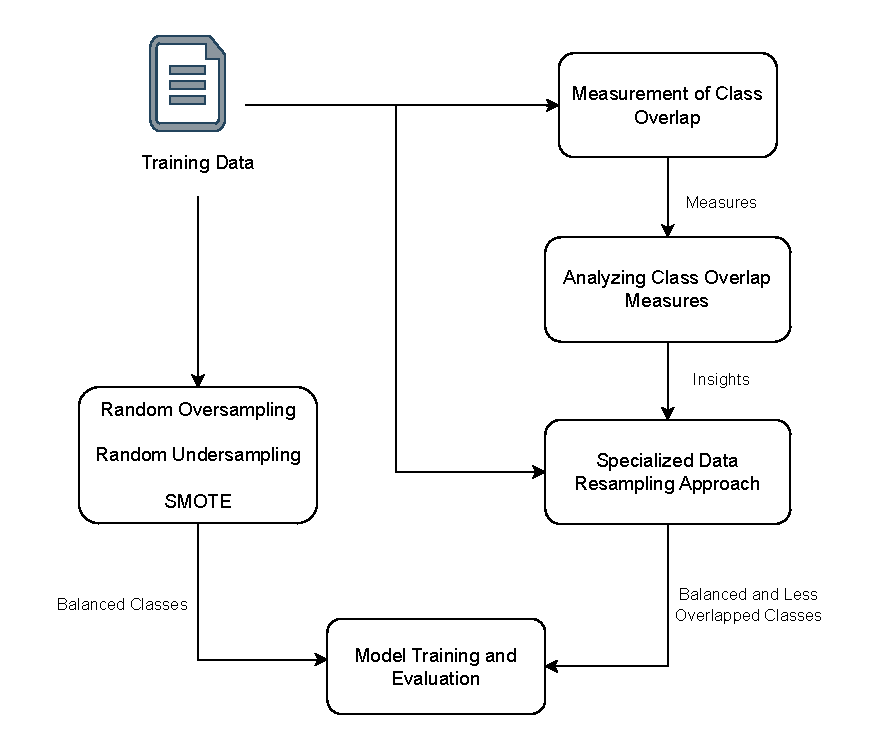
\includegraphics[width=\textwidth]{figures/data-resampling-diagram.pdf}
    \caption{Specialized data resampling approach guided by class overlap measures}
    \label{fig:data-resampling}
\end{figure}

The proposed methodology uses a hybrid data resampling approach, which combines cleaning-based and oversampling methods to address a particular aspect of class overlap. For the cleaning-based component, the Edited Nearest Neighbor (\acrshort{ENN}) method was used \cite{Wilson1972Asymptotic}. ENN works by removing data points from both classes that are considered noisy or mislabeled. It works by checking nearest neighbors of each data point. Data points were removed if the majority of their neighbors belong to a different class. This step helps to clean up the data by removing examples that fall on the wrong side of the decision boundary. Thus, it reduces noise and class overlap. 

The choice of the oversampling method depends on the region of class overlap. The K-means Synthetic Minority Over-sampling Technique (\acrshort{KMeansSMOTE}) \cite{Douzas2018Improving} was used to handle structural class overlap by boosting the safe and sparse regions of the minority class. It uses k-means clustering to group similar minority class instances together and then applies the Synthetic Minority Over-sampling Technique (\acrshort{SMOTE}) algorithm to generate new synthetic examples only within these specific clusters. This could create more meaningful and representative new data points, rather than producing synthetic examples in areas where they might be less helpful. The other oversampling method used in this study is \acrshort{BorderlineSMOTE} \cite{Han2005Borderline-SMOTE}. This method introduces new minority class examples in areas that are located around the decision boundary between different classes. This approach effectively strengthens the minority side of the overlapped border. As a result, it becomes easier for a model to accurately classify the minority class examples.

\hl{The combination of SMOTE with data cleaning methods, were proven by} \cite{Sharma2024Leveraging} \hl{to successfully reduce selection bias and significantly improve the classification accuracy of dementia subtypes. The hybrid data resampling approach was also evaluated in a critical review} \cite{Santos2022Joint}. \hl{Furthermore, the use of class overlap measures as metadata to guide data resampling is recognized by a recent review} \cite{Santos2023Unifying} \hl{as an effective strategy to overcome complex imbalanced data domains. The elimination of negative instances specifically in overlapping regions was proven by} \cite{Vuttipittayamongkol2020Improved} \hl{to significantly enhance sensitivity and overall classification performance in neurodegenerative disease datasets. Similarly,} \cite{Kraiem2021Selecting} \hl{demonstrated that the most effective data resampling strategy must be systematically guided by the intrinsic overlap and imbalance characteristics of the data rather than applying a universal method. Although some of these specific studies were not conducted using the identical clinical datasets of this research, the application of this approach is supported by their solid findings.}

The algorithm used to decide the suitable data resampling is presented in Algorithm \ref{alg:data-resampling}. Firstly, the imbalance ratio (\acrshort{IR}) and the class overlap measures (kDN and N1) are calculated based on the training dataset. After that, the algorithm checks for class overlap (kDN > 0.3 or N1 > 0.3) or moderate imbalance classes (IR > 2.0). Data resampling is skipped if neither class imbalance nor class overlap exists. On the other hand, if class overlap is found, ENN is applied to the training dataset to clear the overlapped instances and potential mislabeled examples in both classes. After that, the percentage of borderline examples for both classes is computed. This is followed by oversampling of the minority class using BorderlineSMOTE if the minority class is less represented around the class boundaries or KMeansSMOTE otherwise. This selection of the oversampling method ensures that the synthetic examples are added to sparse regions of the minority class. In cases where class imbalance exists without class overlap, oversampling is applied only without data cleaning using ENN.

\captionsetup[algorithm]{list=no}
\begin{algorithm}
\caption{Data Resampling Decision Algorithm}
\label{alg:data-resampling}
\begin{algorithmic}[1]
    \Require Training dataset $D$ with minority class $C_{min}$ and majority class $C_{maj}$
    \Ensure Resampled training dataset $D'$ or original training dataset $D$
    
    \State Compute $IR \leftarrow \frac{|C_{maj}|}{|C_{min}|}$
    \State Compute $kDN$ (k-Disagreeing Neighbours measure)
    \State Compute $N1$ (Fraction of Borderline Points measure)
    
    \If{$kDN > 0.3$ or $N1 > 0.3$ or $IR > 2.0$}
        \If{$kDN > 0.3$ or $N1 > 0.3$}
            \Comment{Apply ENN to $D$}
            \State $D \leftarrow ENN(D)$
        \EndIf

        \State Compute $BE_{min}$ (Percentage of Borderline Examples in $C_{min}$)
        \State Compute $BE_{maj}$ (Percentage of Borderline Examples in $C_{maj}$)
    
        \If{$BE_{min} < BE_{maj}$}
            \Comment{Apply BorderlineSMOTE to $D$}
            \State $D' \leftarrow \text{BorderlineSMOTE}(D)$
        \Else
            \Comment{Apply KMeansSMOTE to $D$}
            \State $D' \leftarrow \text{KMeansSMOTE}(D)$
        \EndIf
        \State \Return $D'$
    \Else
        \Comment{Skip data resampling}
        \State \Return $D$
    \EndIf
\end{algorithmic}
\end{algorithm}

To evaluate the chosen resampling method, the method is subsequently used to train a RF model in stratified cross-validation. RF was chosen because it demonstrates consistent behavior with imbalanced datasets. It also reduces the risk of overfitting, which could favor certain balancing approaches. The performance of the RF model is then compared with the baseline (without data resampling) and common resampling methods: random undersampling, random oversampling, and SMOTE \cite{Chawla2002SMOTE}. This evaluation assesses the geometric mean (\acrshort{G-mean}) and the recall of both binary classes. A data resampling method that improves the accuracy of the minority class and provides a balanced performance between both classes is selected. The data resampling methods were implemented using the imbalanced-learn library version 0.12.4 \cite{Lematre2016Imbalanced-learn}.

% By combining these two techniques, the hybrid method first cleans the data with ENN and then selectively generates new samples with KMeansSMOTE or BorderlineSMOTE in the targeted regions based on the identified overlap characteristics. This targeted, two-stage methodology is proposed to be more effective than generic methods like random oversampling or standard SMOTE. Generic approaches possess no mechanism that can handle class overlap and may worsen the problem by generating new data points within already overlapped regions.

This methodology is especially useful in the context of this study, which uses accessible data to train classification models. This is because these features have a relatively low degree of predictability of the target classes. It becomes important to avoid increasing class overlap by applying random or generic data resampling. This ensures that quality data are ready to be used for model training and fine-tuning, which are discussed in the following section.

\section{Model Fine-Tuning and Selection}
Following data preprocessing, feature selection, and data resampling, the subsequent section of the research methodology focuses on fine-tuning and selection of machine learning models. The main objective of this study is to develop cost-effective models capable of accurately classifying cognitive status and CI subtypes. \hl{For this reason, the model selection is designed to choose efficient models that reduce the cost of training and prediction, which is one of the main components of the cost-effective methodology.} The model selection works by employing a two-stage process as explained in the following subsections.

\subsection{Classification Models}
The models evaluated in this study include Logistic Regression (\acrshort{LR}), k-Nearest Neighbors (\acrshort{KNN}), Support Vector Machines (\acrshort{SVM}) with Radial Basis Function (\acrshort{RBF}) kernel, Random Forest (\acrshort{RF}), and Light Gradient Boosting Machine (\acrshort{LightGBM}). This set of models were chosen for several key reasons. These models are widely recognized in the machine learning literature for their robust performance and are commonly employed in similar healthcare and biomedical research domains. \hl{Beyond this reason, the selection of these models is also supported by their theoretical properties and how these properties suit the nature of the data in this study. LR is a linear model with low complexity that assumes a linear relationship between the features and the log-odds of the outcome} \cite{Hastie2009Elements}. \hl{It is stable and easy to interpret, and it is theoretically expected to generalize well when the feature space is small and the class overlap is reduced. KNN is a non-parametric and distance-based model that classifies a subject according to its nearest neighbors} \cite{Cover1967Nearest}. \hl{It can capture local patterns in the data, but it becomes less effective in high-dimensional or highly overlapping data. SVM with an RBF kernel separates the classes by finding the maximum-margin boundary in a higher-dimensional space to model non-linear relationships, while its regularization parameter controls overfitting} \cite{Cortes1995Support}. \hl{RF is a tree-based ensemble that combines multiple decision trees through bagging to reduce variance and to capture feature interactions and non-linear effects} \cite{Breiman2001Random}. \hl{LightGBM is a gradient boosting ensemble that builds trees sequentially to reduce bias and to model complex interactions efficiently, but its higher complexity makes it more prone to overfitting in small or overlapping data} \cite{Ke2017LightGBM}.

\hl{Therefore, the selected models cover a range of complexity, from linear and distance-based classifiers to non-linear and tree-based ensemble methods. This allows the study to examine whether simpler and more cost-effective models can achieve a performance that is comparable to or better than complex ensembles once the feature space is reduced and the class overlap is minimized.} This evaluation provides valuable insights into the models' suitability for the specific problem of this research. These models are systematically fine-tuned in this study to find the best hyperparameters that produce cost-effective classifiers.

The methodology works by employing a two-stage process. The first stage is model fine-tuning using Grid Search hyperparameter tuning for all five classification algorithms. This step creates a large pool of tuned models for each algorithm. Next, a novel cost-effective selection algorithm (explained in section \ref{sec:cost-effective-model-selection-algorithm}) is applied to the optimized models to select the most cost-effective model of each classification algorithm. This results in five finalist models for each classification task in this study. In the second stage, an assessment of the shortlisted models is conducted. This assessment compares models based on their overall performance, computational efficiency, and interpretability (the degree to which humans can understand and explain why a machine learning model makes a specific prediction or decision). This evaluation leads to the selection of the best model for each classification task.

\subsection{Model Hyperparameters Fine-Tuning}
% The fine-tuning of hyperparameters for each model is not a blind search but is systematically guided by the insights derived from the class overlap analysis. The effectiveness of a model's hyperparameters is often contingent upon the specific nature of the class overlap \cite{Santos2022Joint}. A single set of hyperparameters may not be optimal for a dataset characterized by structural overlap as opposed to one with instance-level overlap. the methodology, therefore, leverages the meta-knowledge gained from class overlap measures to inform the hyperparameter search space. For example, in domains where class overlap is dominated by noisy or hard-to-classify instances (instance-level overlap), tuning hyperparameters that control model regularization (such as the C parameter in SVM or the L1/L2 penalties in LR) becomes critical. These parameters directly influence the model's capacity to handle mislabeled or borderline instances. Conversely, in datasets with high structural overlap, where minority clusters are scattered within the majority class manifold, models that are sensitive to local data density, such as KNN, require careful tuning of parameters like k to optimize performance. For ensemble models like Random Forest the tuning of parameters such as tree depth, and the number of estimators is guided by the need to create models that are not overly complex and are robust to the specific types of overlap identified. This data-driven, complexity-aware hyperparameter tuning method improves predictive performance and generalizability by making the search process more efficient and more likely to produce an accurate model.
For each classification task, model hyperparameter fine-tuning was performed in stratified 5-fold cross-validation. The selection of the best-tuned model for each of the modeling algorithms is based on a combined evaluation of the model's performance and efficiency. The model's ability to provide accurate classification was evaluated using appropriate performance metrics suitable for the classification task. A combination of F1-score and G-mean metrics was used for the four cognitive status classification and prediction tasks, while G-mean only was used in the CI subtype classification task. The efficiency of the model was measured based on its training and prediction speed. A slow model increases development lead time and operational costs, particularly if the model is deployed on the cloud infrastructure. Therefore, the speed of the model is an essential metric in this study to develop cost-effective models. The training throughput (the total number of samples the model can learn per second) of the model was calculated by dividing the total number of training samples by the mean time taken to invoke the model \textit{fit} method over 5-fold cross-validation iterations. Similarly, the prediction throughput (the total number of predictions the model can make per second) was computed by dividing the total number of validation samples by the mean execution time of the model's \textit{predict} method.

To ensure a fair comparison, all models were fine-tuned and trained using the e2-standard-8 virtual machine on the Google Cloud Platform. The machine is configured with eight virtual centralized processing units, 32 gigabytes of memory, and a fifth-generation Intel processor (Intel Broadwell) with no graphics processing units allocated. To train and evaluate the models, Python version 3.11.2 and several Python libraries were used. This includes Scikit-learn 1.5.2 and lightgbm 4.6.0.

\subsection{Model Selection}
Optimizing models to achieve high cost-effectiveness is not an easy task. It requires the evaluation of multiple performance and efficiency metrics to select the best set of hyperparameters that balance between model accuracy and efficiency. Therefore, a novel algorithm was developed to automate the selection of hyperparameters to reduce the cost of training and operating the models by improving their training and prediction speeds while maintaining acceptable performance levels. The following subsection explains the cost-effective model selection algorithm.

\subsubsection{Cost-effective Model Selection Algorithm}
\label{sec:cost-effective-model-selection-algorithm}
The proposed selection algorithm selects the best model from the based on a cost and performance trade-off. This algorithm is used to select the best cost-effective model for each classification algorithm based on hyperparameter optimization. The cost and performance trade-off considers the model's performance and the cost associated with training and using the model. The performance of the model was evaluated using a single metric or a combination of performance metrics. The cost of the model was assessed using the model speed, which was measured using the training and prediction throughputs. The logic of the selection algorithm can be divided into three phases. The first phase determines a benchmark model, the second phase uses the benchmark to filter the other models, and the third phase selects the best model that balances speed and performance. Algorithm \ref{alg:model-selection} explains the logic of this algorithm.

\floatname{algorithm}{Algorithm}
\begin{algorithm*}
\caption{The Cost-effective Model Selection Algorithm}
\label{alg:model-selection}
\small
\begin{algorithmic}[1]
    \State Define the array of performance metrics: $p$
    \State Define weights of the performance metrics: $w$
    \State Define the training throughput weight: $W\textsubscript{trn}$
    \State Define the prediction throughput weight: $W\textsubscript{pred}$
    \State Define thresholds of the accepted performance decrease: $T\textsubscript{$p$}$
    \State Define a threshold of relative change in training throughput: $T\textsubscript{trn}$
    \State Define a threshold of relative change in prediction throughput: $T\textsubscript{pred}$
    
    \For{each model $(m)$ in the collection of models}
        \State Calculate $\bar{w}_p$: weighted average of the performance metrics of $m$ \Comment{Equation \eqref{eq:performance-avg}}
    \EndFor
    
    \State Find a benchmark model $B$: the model with the largest weighted average performance $\bar{w}_p$ 
    \State $B\textsubscript{$\bar{w}_p$} \gets the\ weighted average performance\ of\ B$
    \State $B\textsubscript{trn} \gets the\ training\ throughput\ of\ B$
    \State $B\textsubscript{pred} \gets the\ prediction\ throughput\ of\ B$
    
    \For{each model $(m)$ in the collection of models}
                
        \If{B\textsubscript{$\bar{w}_p$} - m\textsubscript{$\bar{w}_p$} <= T\textsubscript{$p$}}
            
            \State $m\textsubscript{trn} \gets the\ training\ throughput\ of\ m$
            \State Calculate $\Delta$trn the relative change $m\textsubscript{trn}$ from $B\textsubscript{trn}$ \Comment{Equation \eqref{eq:train-speed-increase}}
            
            \State $m\textsubscript{pred} \gets the\ prediction\ throughput\ of\ m$
            \State Calculate $\Delta$pred the relative change $m\textsubscript{pred}$ from $B\textsubscript{pred}$ \Comment{Equation \eqref{eq:pred-speed-increase}}
            
            \If{$\Delta$trn > T\textsubscript{trn} AND $\Delta$pred > T\textsubscript{pred}} 
                \State Calculate the relative speed of $m$ ($m\textsubscript{speed}$) \Comment{Equation \eqref{eq:speed-weighted-avg}}
            \Else
                \State $m$ is excluded because its relative change in speed is below the defined thresholds                
            \EndIf
            
        \Else
             \State $m$ is excluded because its weighted average performance reduction exceeds the defined threshold
        \EndIf
    \EndFor
        
    \State Select the model with the highest speed $m\textsubscript{speed}$
    
\end{algorithmic}
\end{algorithm*}

In the first phase (lines 8-10) of the algorithm, the weighted average of the performance metrics ($\bar{w}_p$) was calculated to define the performance of each model. Refer to equation \eqref{eq:performance-avg}. Performance metrics (\textit{p}) and their weights (\textit{w}) are predefined values. The model with the highest value of $\bar{w}_p$ is selected as the initial best-performing model (line 11). This model is used as a benchmark model in the second phase to filter the other models based on two criteria.

\begin{equation}
    \bar{w}_p = \frac{\sum_{i=1}^{n} (p_i \cdot w_i)}{\sum_{i=1}^{n} w_i}
    \label{eq:performance-avg}
\end{equation}
Equation (\ref{eq:performance-avg}) calculates the weighted average of the model performance metrics, where
\begin{itemize}
    \item $p_i$ is the value of the performance metric at index \textit{i}.
    \item $w_i$ is the weight of the performance metric at index \textit{i}. 
    \item $n$ is the total number of performance metrics.
\end{itemize}
\vspace{2em}

The first criterion in the second phase (line 16) pertains to a decrease in the model performance. This ensures that a model is qualified only if its reduction in weighted average performance, compared to the benchmark model, does not exceed a predefined threshold (\textit{T\textsubscript{p}}). The second criterion (line 21) is related to the change in the speed of the model. The relative change in the training throughput is calculated using equation \eqref{eq:train-speed-increase}, while the relative change in the prediction throughput is calculated using equation \eqref{eq:pred-speed-increase}. Models are qualified only if their relative changes in the training and prediction throughputs from the benchmark model's throughputs are higher than the predefined thresholds (\textit{T}\textsubscript{trn}) and (\textit{T}\textsubscript{pred}), respectively. 

If no model meets both criteria of the filtering phase, the benchmark model is selected as the most cost-effective model. Otherwise, in the third phase (line 22), the relative speed of each qualified model is calculated as the weighted average of the relative change in the training and prediction throughputs using the predefined weights for the training throughput (\textit{W}\textsubscript{trn}) and the prediction throughput (\textit{W}\textsubscript{pred}). Refer to equation \eqref{eq:speed-weighted-avg}. Finally, the model with the highest relative speed is selected as the most cost-effective based on the required cost and performance trade-off.

\begin{subequations}\label{eq:speed-increase}
    \begin{align}
        \label{eq:train-speed-increase}
        \Delta \text{trn} = \frac{\left( m_{\text{trn}} - B_{\text{trn}} \right)}{B_{\text{trn}}} \\
        \label{eq:pred-speed-increase}
        \Delta \text{pred} = \frac{\left( m_{\text{pred}} - B_{\text{pred}} \right)}{B_{\text{pred}}}
    \end{align}
\end{subequations}
Equation \eqref{eq:train-speed-increase} calculates the relative change in the training throughput $\Delta{\text{trn}}$ of a given model \textit{m}\textsubscript{trn} from the benchmark training throughput \textit{B}\textsubscript{trn}. In \eqref{eq:pred-speed-increase}, the same equation is used to calculate the relative change in the prediction throughput $\Delta{\text{pred}}$, where \textit{m}\textsubscript{pred} is the prediction throughput of the given model, and \textit{B}\textsubscript{pred} is the prediction throughput of the benchmark model. The relative change in throughput is positive if the given model is faster than the benchmark model or negative otherwise.

\begin{equation}
    m_{\text{speed}} = \frac{\left(\Delta \text{trn} \cdot W_{\text{trn}} + \Delta \text{pred} \cdot W_{\text{pred}}\right)}{W_{\text{trn}} + W_{\text{pred}}}
    \label{eq:speed-weighted-avg}
\end{equation}
\textit{m}\textsubscript{speed} is the weighted average of the relative change in the training throughput $\Delta{\text{trn}}$ and prediction throughput $\Delta{\text{pred}}$, where \textit{W}\textsubscript{trn} is the training throughput weight and \textit{W}\textsubscript{pred} is the prediction throughput weight.
\\

\begin{table*}[!ht]
    \centering
    \scriptsize
    \caption{The cost-effective model selection algorithm parameter values}
    \newcolumntype{C}{>{\centering\arraybackslash}X}

        \begin{tabularx}{\textwidth}{|C|C|C|C|C|}
        % \begin{tabularx}{\textwidth}{|m{2cm}|X|X|X|p{1.75cm}|}
        \hline
            \textbf{Parameter} & \textbf{Description} & \textbf{Value Determination Question} & \textbf{Accpeted Value} & \textbf{Assigned Value } \\ \hline
            \textbf{Performance Metrics\textsuperscript{1}} & Metrics used to evaluate model performance. & What specific aspects of model performance are critical to the business or research objectives? & A metric name or list of metrics names & ["F1-score", "G-mean"] or ["G-mean"]  \\ \hline
            \textbf{Weights for Metrics} & Importance assigned to each performance metric. & How is the importance of each performance metric to be prioritized in achieving the business or research objectives? & An array of positive numbers associated with the performance metrics. It can be unassigned to apply the same weight to all metrics or when one metric is used. & [2, 1]  \\ \hline
            \textbf{Performance Thresholds} & The accepted decrease in performance (based on the weighted average performance). & What level of decrease in performance is acceptable for the use case? & A numerical value between zero (0) and one (1). & 0.02  \\ \hline
            \textbf{Training Throughput Threshold\textsuperscript{2}} & The minimum percentage of change in training speed. & What percentage of change in training speed is required for the use case? & A numerical value representing the percentage of change in training speed. & 0.0  \\ \hline
            \textbf{Prediction Throughput Threshold\textsuperscript{2}} & The minimum percentage of change in validation speed. & What percentage of change in prediction speed is required for the use case? & A numerical value representing the percentage of change in prediction speed. & 0.0  \\ \hline
            \textbf{Training Throughput Weight} & Importance of training speed in relative speed calculation. & How should the importance of training speed be weighed against prediction speed in achieving the business or research objectives? & Positive number. & 1  \\ \hline
            \textbf{Prediction Throughput Weight} & Importance of prediction speed in relative speed calculation. & How should the importance of prediction speed be weighed against training speed in achieving the business or research objectives? & Positive number. & 2  \\ \hline
            \multicolumn{5}{p{400pt}}{\footnotesize \textsuperscript{1}The assigned value of the performance metrics depends on the classification task. A combination of F1-score and G-mean metrics is used for the four cognitive status classification and prediction tasks, while G-mean only is used in the CI subtype classification task.\newline
            \textsuperscript{2}Either the value of the training or prediction throughput thresholds can be a negative number representing an acceptable decrease in speed, but not both. For example, a use case that requires an increase in prediction throughput with no concern about the decrease in training throughput can define a negative training throughput threshold and a positive prediction throughput threshold.}
        \end{tabularx}
    \label{table:algorithm-parameters}
\end{table*}

The proposed model selection algorithm is highly versatile and can be customized to fit a wide range of use cases beyond the scope of this study. The algorithm allows users to define and customize performance metrics based on their business objectives. By translating business performance and efficiency requirements into weights and thresholds, users can utilize the algorithm to select the best models that meet their unique needs. The effectiveness of the algorithm output relies heavily on the appropriate parameter values. To meet the objectives of this study, the parameters of the cost-effective model selection algorithm were configured to develop an efficient prediction model with minimal impact on the performance of the model. Table~\ref{table:algorithm-parameters} provides a detailed view of the values of the parameter values of the model selection algorithm used for the classification tasks in this research. The goal was to select hyperparameters that result in a model with higher training and prediction throughputs than the benchmark model (the best-performing model) while maintaining a performance level that is at most 2 percentage points lower than the benchmark model. Prediction throughput was prioritized over training throughput to create a resource-efficient and scalable solution that is accessible to a broad range of individuals, considering that model updates are infrequent in the context of CI prediction.

Following the optimization of the models' hyperparameters, the best model for each classification task was selected by assessing the models in terms of their performance, efficiency, and interpretability. The final model was then externally validated using the holdout NACC and ADNI external validation datasets. The external validation is explained in the next section. Moreover, the explainability of the final models were assessed to measure feature contributions to models' predictions and to generate useful insights for risk management and intervention.

\section{Model Validation}
\label{sec:model-validation}
A robust model validation methodology was designed with comprehensive assessments of the performance of the models, as illustrated in Figure~\ref{fig:model-validation}. The method consisted of two main phases, the internal validation phase and the external validation phase. \hl{This design involved splitting the NACC UDS dataset of each binary classification task into training and testing datasets based on ADRCs, utilizing a leave-multiple-center-out approach rather than a standard random split. In other words, the NACC training dataset was collected from research centers that were not involved in the collection of the holdout NACC cross-center testing dataset. The proportion of the holdout testing dataset is approximately 20\% in all five classification tasks. This strict separation is crucial to prevent indirect data leakage, which frequently occurs in standard random splitting when subjects from the same center share identical clinical protocols and diagnostic procedures. Furthermore, a NACC UDS-based study} \cite{Phongpreecha2023Prediction} \hl{has successfully utilized a similar center-based data splitting approach.}

The training dataset was utilized in the internal validation phase to develop and validate the fine-tuned models using stratified 5-fold cross-validation. Eventually, the generalizability of the selected models were tested in the external validation phase. The NACC cross-center testing dataset was used to examine the models' performance across ADRCs. Moreover, a second external validation was performed using the ADNI dataset to evaluate the models' generalizability to unseen data. Testing using the ADNI dataset was performed only for all four cognitive status classification and prediction tasks. The ADNI external validation was not done for the AD vs. non-AD classification task because ADNI’s enrollment and exclusion criteria focus on AD and explicitly exclude other causes of dementia. Therefore, ADNI lacks sufficient non-AD examples for a reliable external validation.

\begin{figure}[ht]
    \centering
    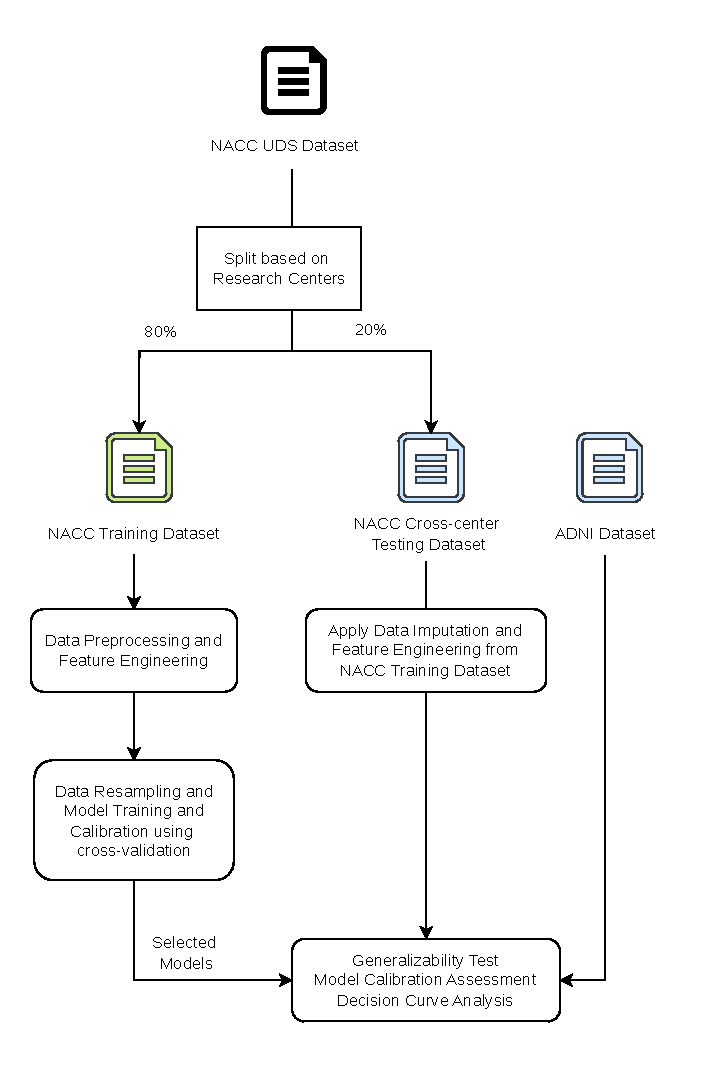
\includegraphics[width=0.65\textwidth]{figures/model-evaluation-diagram.pdf}
    \caption{Diagram of the model validation methodology and the dataset splitting strategy}
    \label{fig:model-validation}
\end{figure}

A deliberate selection of the model performance metrics is important for a reasonable evaluation of the classification models' performance. It can be observed that the datasets of all the binary classification tasks exhibit an imbalanced class distribution. Consequently, this study utilized a combination of performance metrics that account for class imbalance, such as sensitivity, specificity, G-mean, Area Under the Curve (\acrshort{AUC}), and F1-score. This is important to ensure a fair assessment of model performance in both majority and minority classes. In the medical field, it may also be more expensive to misclassify one class than the other. For example, classifying cognitively impaired cases as normal cases has a greater impact than classifying normal cases as cognitively impaired. Therefore, it is advisable to assess the true positive rate of the classification model. The distribution of the target classes in the NACC UDS and ADNI datasets for all classification tasks is provided in Figure~\ref{fig:nacc-data-stat} and Figure~\ref{fig:adni-data-stat} in the appendix, respectively.

In addition to evaluating the generalizability of the selected models, it is important to ensure that the models produce reliable probabilities of the targeted cognitive status or CI type (outcome). There is a possibility that even though a model with high classification accuracy could predict overly confident or conservative risk probabilities. In clinical application, an accurate estimate of how the outcome could possibly occur is required to make the right decision to manage any potential risk. Therefore, it is crucial that the predicted probability of the model approximates the actual likelihood of the outcome. For example, if a model predicts that there is an 80\% chance of cognitive impairment, about 80\% of subjects who get that prediction should have cognitive impairment.

Calibration was applied to the selected model using the beta calibration method to align their predicted probabilities with the actual risk of the outcome. The beta calibration works by fitting three parameters that learn how to transform the model's predicted probabilities to better match the actual likelihood of the risk. This method is more flexible than other approaches because it can correct both overconfidence and underestimation across different probability ranges. 

The beta calibration parameters were fitted using the model prediction in the stratified cross-validation out-of-fold (OOF). During the cross-validation, the model makes predictions on the validation fold (data it did not see during training). These OOF predictions were collected and used to train the beta calibration parameters. This ensures that the calibration is learned from unbiased model output. After that, the learned parameters were used to calibrate the model's predicted probabilities in external validation.

The effectiveness of the calibration was evaluated by comparing the uncalibrated and calibrated models in the NACC cross-center validation and the ADNI external validation using the following measures. These measures together provide a complete assessment of how well the model is calibrated.

\begin{itemize}
    \item \textbf{Calibration Curve:} A visual representation of the relationship between the model's predicted probabilities and the actual risk (diagonal line). A curve that follows the diagonal line indicates that the model is well calibrated. The calibration curve can help assess at which probability ranges the model is overconfident or underestimating the risk.
    \item \textbf{Brier score:} This is a widely used metric that evaluates the accuracy of the probabilities that the model predicts. It is calculated by taking the mean squared difference between the predicted probabilities and the actual outcomes. A Brier score below 0.20 means that the model prediction is accurate and calibrated.
    \item \textbf{Expected Calibration Error (\acrshort{ECE}):} This score measures the difference between the predicted probabilities and the observed frequencies. To calculate ECE, the model's predictions are divided into 10 bins. Then, the score is obtained by the weighted average of absolute differences between the mean predicted probability and the actual outcome frequency in each bin. In general, ECE values close to and below 0.05 indicate good calibration.
    \item \textbf{Intercept and Slope:} These values are obtained by a logistic regression model fitted to the calibration curve. An intercept below 0 indicates that the predicted probabilities are higher than the actual risk (the model is overestimating the risk), whereas an intercept above 0 indicates that the predicted probabilities are less than the actual risk (the model is underestimating the risk). The slope measures how well the model differentiates between different risk levels. A slope below 1 means the model is overconfident, pushing the predicted probabilities closer to 0 and 1, whereas a slope above 1 means the model is underconfident as it compresses probabilities around middle values (between 0.3 and 0.7). An intercept close to 0 and a slope close to 1 are considered measures of good calibration.
\end{itemize}
\vspace{2em}

After model calibration, the clinical utility of all classification and prediction models were assessed using Decision Curve Analysis (\acrshort{DCA}). This was done by calculating the model’s net benefit for different probability thresholds. DCA evaluates whether using these probabilities to guide clinical decisions provides additional value compared to alternative strategies like treat all and treat none.

\hl{This proposed validation method complies with the TRIPOD+AI guidelines} \cite{Collins2024TRIPOD+AI} \hl{through its focus on external validation, calibration, and clinical utility. Instead of relaying only on mathematical metrics, the predicted probabilities were assessed with calibration curves and clinical value was examined through decision curve analysis. Furthermore, the leave-multiple-center-out splitting follow recommendations from the literature} \cite{Christodoulou2019systematic}, \hl{which reported that validation procedures of machine learning models in clinical prediction are often biased and rarely calibrated.}

\section{Model Explainability}
The utility of a predictive model in a clinical setting goes beyond only prediction. It is necessary for the model prediction to be transparent, interpretable, and actionable. Since the objectives of this study are centered on the development of models that not only predict CI but also support personalized intervention plans, an XAI approach to model explainability is essential. 

The proposed XAI method in this study provides model explainability at multiple levels. The SHapley Additive exPlanations (\acrshort{SHAP}) \cite{Lundberg2017Unified} was used to provide global and individual explanations of the models’ predictions. This method computes Shapley values to quantify the contribution of each feature to a single model's prediction. For global explanation, the mean absolute Shapley values of each feature were calculated to determine the overall feature importance to the selected model. These values can be used to rank the features according to their overall importance to the model's prediction. This global explanation of the models is important to identify which risk factors (features) are the most strongly linked to cognitive impairment across the whole population. The feature importance was calculated on the ADNI external dataset, and it was compared to the feature importance on the NACC cross-center validation dataset using Spearman correlation. This comparison evaluates the stability of feature ranking across different datasets, which could demonstrate the generalizability of the model and the selected features.

In addition to the global explanation, the Shapley values were also used to explain the model prediction of individual instances. This local-level explanation clarifies why a specific instance got a particular prediction from the model. It helps answer questions like "What factors contributed to a case being classified as positive or negative?" which supports personalized risk communication and intervention. Shap waterfall plots were reported to demonstrate how correctly classified positive and negative cases with similar prediction probabilities have different feature contribution profiles. This assesses the capability of the selected model to capture specific risk patterns for different subjects. Although other local explanation methods like \acrshort{LIME} (Local Interpretable Model-agnostic Explanations) are used in the literature \cite{abbas2024Explainable, Vyas2022Identifying}, SHAP was utilized in this study because it is already used to compute the feature importance, and it has been widely used for global and individual explanation by other studies in CI and dementia research \cite{Beebe-Wang2021Efficient, Danso2021Developing, Yue2023Explainable}.

The XAI method in this study also leverages Diverse Counterfactual Explanations (\acrshort{DiCE}) \cite{Mothilal2019Explaining} to generate patient-specific counterfactual insights for risk management and intervention. For subjects predicted to have CIND or dementia, DiCE can propose a set of changes to their modifiable features that would be required to change the model's prediction to a desirable prediction (less severe cognitive status). A key advantage of DiCE is its ability to be configured to suggest changes only for features that can be modified (e.g., functional activities or scores from a Geriatric Depression Scale (\acrshort{GDS})), while keeping features such as gender and age static. For example, DiCE might suggest that a patient's cognitive status could improve from impaired to normal by managing the patient's GDS. This addresses this research objective to support the development of personalized risk management strategies. This counterfactual explanation was applied to all classification and prediction tasks in this study except the CI subtype classification task because the conversion from one CI subtype to another has no clinical value.

DiCE works by searching for different feature values that are similar to the original instance but result in different prediction outcomes. The goal is to minimize the distance between the original and counterfactual instances while ensuring that the desired outcome is obtained. In this research, the \acrshort{KD-Tree} (K-dimensional tree) search method was used to generate the counterfactual examples. This method builds a tree structure from the training data to search for nearest neighbors in the feature space that belong to the desired prediction class. The KD-Tree method was selected because it generates counterfactual examples that are based on real instances (training data) instead of generating synthetic examples that might not be feasible in practice. Additionally, it is computationally efficient for large datasets.

In this study, DiCE was configured to generate up to five counterfactual examples for each instance predicted as positive. The number of counterfactual examples generated per instance was analyzed to assess the ability of DiCE to find possible changes to improve cognitive status. The total number of features changed to generate counterfactual examples was also examined to evaluate the difficulty in applying the suggested interventions. DiCE also provides global importance scores for each feature based on how frequently it needs to be modified across all generated counterfactual examples. These scores were used to identify the most important features that could be utilized for risk interventions. Permitted values for certain features were defined, which were used by DiCE to generate realistic counterfactual examples. For example, the mass body index feature (NACCBMI) was configured with allowed values between 18.5 and 24.9, whereas the "never did" value in the FAQ features was set as disallowed.

In summary, the proposed XAI method was designed to provide both a global understanding of the selected models and patient-specific insights for CI risk prevention. It is achieved by the integration of SHAP for global feature importance and individual prediction explanations and DiCE for counterfactual insights. Consequently, the output of the models were transformed into a clinically meaningful and justifiable outcome. Therefore, it increases confidence in the model prediction and builds trust among clinicians and patients.

\hl{The results obtained from applying this methodology to the five classification and prediction tasks are presented and analyzed in the following chapter.} % Methodology
%!TEX ROOT = thesis.tex
\chapter{Results and Analysis}

\hspace{12.7mm}This chapter presents the results of the research work. The results are analyzed in detail to provide insights into the findings and their implications for the study. The chapter is organized into three main sections. Each section presents the related results that support the research objectives of developing cost-effective machine learning models to predict the risk of cognitive impairment and classify its etiology.

\section{Current Cognitive Status Classification Results}
This section presents the results for the first research objective, which focuses on developing cost-effective models to classify current cognitive status. The section provides results for the normal cognition (\acrshort{NC}) vs. cognitive impairment (\acrshort{CI}) prediction task and the cognitive impairment but not dementia (\acrshort{CIND}) vs. dementia prediction task.

\subsection{Feature Selection Results}

This subsection presents the results of the feature selection for the two classification tasks. The proposed feature selection method is based on the ensemble feature ranking methods and the automatic feature selection threshold using a class overlap measure. 

To evaluate this method, the results were compared with the baseline and the Boruta algorithm. The evaluation was performed using a random forest (\acrshort{RF}) model in internal cross-validation. The goal was to find a subset of features that reduces the data complexity and improves the computational efficiency while maintaining a high level of predictive performance. Several metrics were used to compare the methods. These include the number of selected features, the class overlap (Maximum Fisher's Discriminant Ratio (\acrshort{F1})), and the model's predictive performance measured using the geometric mean (\acrshort{G-mean}).

\subsubsection{Feature Selection Results for the NC vs. CI Classification Task}\label{sec:feature-selection-task1}

As shown in Table~\ref{table:fs-task1}, the proposed feature selection method successfully identified a minimal and cost-effective subset of features. The baseline model, which was based on the initial 68 features, achieved the highest predictive performance with a G-mean of 0.840. However, it had high data complexity (0.946 F1 feature overlap score) and lowest computational efficiency. The proposed method selected only 12 features. This is an 82\% reduction from the baseline and also fewer than the 15 features selected by the Boruta method. This minimal feature set had only a minor acceptable impact on predictive performance, achieving a G-mean of 0.829. This score is competitive with both the baseline and the Boruta method.

\begin{table}[!ht]
    \centering
    \caption{Comparison of feature selection methods for the NC vs. CI classification task}
    \begin{tabular}{|c|c|c|c|c|}
    \hline
        Method & Number of Features & G-mean & Fitness Score & F1 \\ \hline
        Baseline & 68 & 0.840 & 0.700 & 0.946 \\ \hline
        Boruta & 15 & 0.833 & 0.824 & 0.815 \\ \hline
        \textbf{Proposed Method} & \textbf{12} & \textbf{0.829} & \textbf{0.828} & \textbf{0.788} \\ \hline
        \multicolumn{5}{p{400pt}}{\footnotesize \hl{F1: Fisher's discriminant ratio (feature overlap measure), Fitness Score: combined score balancing performance and feature reduction, G-mean: geometric mean score.}}
    \end{tabular}
    \label{table:fs-task1}
\end{table}

More importantly, the subset of features selected by our method achieved the lowest F1 feature overlap score (0.788). This result indicates that our overlap-guided approach was the most successful in reducing data complexity and improving the separability of classes. This reduction in complexity and feature count translated directly into better efficiency. The model using our selected features had a training throughput of 20,870 samples per second. This is over 2.7 times faster than the baseline model and it also achieved the highest inference speed.

Finally, our proposed method achieved the highest fitness score (0.828), slightly exceeding the Boruta method (0.824), and significantly better than the baseline (0.700). This confirms that our method provided the best overall balance between high performance and model simplicity, which directly answers our research objective to develop a cost-effective solution.

The 12 features selected by the proposed method for the NC vs. CI task are presented in Table~\ref{table:features-task1}. The selected feature set is composed of four categories of accessible data. The majority of the selected features (8 out of 12 features) are assessments of instrumental activities of daily living (\acrshort{IADL}) collected using the Functional Activities Questionnaire (\acrshort{FAQ}). The remaining features include two demographic variables, a memory complaint from the Geriatric Depression Scale (\acrshort{GDS}), and an item from the Neuropsychiatric Inventory Questionnaire (\acrshort{NPI-Q}).

\begin{table}[h!]
\centering
\caption{List of selected features for the NC vs. CI Classification task}
\label{table:features-task1}
\begin{tabular}{ccc}
\toprule
\textbf{Feature Code} & \textbf{Feature Description} & \textbf{Feature Category} \\
\midrule
NACCAGE & Age & Demographics \\
SEX & Sex & Demographics \\
MEMPROB & Subject reported memory problem & GDS \\
BILLS & Pay bills and track spending & FAQ \\
TAXES & Assemble tax records & FAQ \\
SHOPPING & Shop alone for necessities & FAQ \\
GAMES & Play a game of skill & FAQ \\
EVENTS & Keep track of current events & FAQ \\
PAYATTN & Pay attention to a conversation & FAQ \\
REMDATES & Remember dates and appointments & FAQ \\
TRAVEL & Travel out of neighborhood & FAQ \\
ANX & Anxiety in the last month & NPI-Q \\
\bottomrule
\end{tabular}
\end{table}

\subsubsection{Feature Selection Results for the CIND vs. Dementia Classification Task}
Feature selection was also extended to the CIND vs. dementia classification task. The same comparative analysis was performed to evaluate the proposed method against a baseline and the Boruta method. The results of this comparison are illustrated in Table~\ref{table:fs-task2}.

\begin{table}[!ht]
    \centering
    \caption{Comparison of feature selection methods for the CIND vs. dementia classification task}
    \begin{tabular}{|c|c|c|c|c|}
    \hline
        Method & Number of Features & G-mean & Fitness Score & F1 \\ \hline
        Baseline & 71 & 0.833 & 0.694 & 0.941 \\ \hline
        Boruta & 14 & 0.799 & 0.800 & 0.889 \\ \hline
        \textbf{Proposed Method} & \textbf{11} & \textbf{0.815} & \textbf{0.820} & \textbf{0.754} \\ \hline
        \multicolumn{5}{p{400pt}}{\footnotesize \hl{F1: Fisher's discriminant ratio (feature overlap measure), Fitness Score: combined score balancing performance and feature reduction, G-mean: geometric mean score.}}
    \end{tabular}
    \label{table:fs-task2}
\end{table}

The proposed method selected a subset of 11 features. This represents an 84.5\% decrease from the 71 initial features used in the baseline and is also smaller than the 14 features selected by the Boruta method. In terms of the RF model performance, the baseline model had the highest G-mean score of 0.833. The proposed method obtained a G-mean of 0.815. This result was close to the baseline and was also considerably higher than the 0.799 G-mean from the Boruta method. The features selected by the proposed method balance high performance and reduced complexity, which is reflected by the highest fitness score. The fitness score of the proposed method (0.820) exceeded both the Boruta method (0.800) and the baseline (0.694).

The simplicity obtained by the proposed method can be observed in the feature overlap metrics. The proposed method achieved an F1 feature overlap score of 0.754, which was a significant improvement compared to both the Boruta method (0.889) and the baseline (0.941). Additionally, the high ratio of feature reduction resulted in an efficient model. The training process for the 11-feature model was over 2.7 times faster than training with the baseline features.

The 11 features that were selected by the proposed method for the CIND vs. dementia classification task are presented in Table~\ref{table:features-task2}. An analysis of the list shows that 8 out of 11 features are IADL features from the FAQ. The remaining features are primary language, energy scale, and appetite problems.

\begin{table}[h!]
\centering
\caption{List of selected features for the CIND vs. dementia Classification task}
\label{table:features-task2}
\begin{tabular}{ccc}
\toprule
\textbf{Feature Code} & \textbf{Feature Description} & \textbf{Feature Category} \\
\midrule
PRIMLANG & Subject's primary language & Demographics \\
BILLS & Pay bills and track spending & FAQ \\
TAXES & Assemble tax records & FAQ \\
SHOPPING & Shop alone for necessities & FAQ \\
GAMES & Play a game of skill & FAQ \\
MEALPREP & Prepare a balanced meal & FAQ \\ 
EVENTS & Keep track of current events & FAQ \\
REMDATES & Remember dates and appointments & FAQ \\
TRAVEL & Travel out of neighborhood & FAQ \\
ENERGY & Do you feel full of energy? & GDS \\
APP & Appetite and eating changes & NPI-Q \\
\bottomrule
\end{tabular}
\end{table}

The selected feature subset in this task can be compared to the one selected for the previous NC vs. CI task. The selected subsets share seven common FAQ features. However, the subset for the CIND vs. dementia classification task includes the ability to prepare a meal over the ability to pay attention to a conversation and includes different demographic, GDS, and NPI-Q features. More details of the selected features and their correlation results can be found in section \ref{sec:feature-selection-apdx} in the appendix.

\subsection{Data Resampling Results}
\label{sec:resampling_results}
This section presents the results of the data resampling method related to the first research objective. The objective is to develop an accurate classification model for the current cognitive status. These results demonstrate how the proposed data resampling methodology addresses class imbalance and class overlap. Handling these data complexities is important to develop an accurate, balanced, and generalizable model. The overlap-guided resampling methodology was applied to the two classification tasks to achieve this objective. The distribution of the target classes in the National Alzheimer's Coordinating Center (\acrshort{NACC}) Uniform Data Set (\acrshort{UDS}) and ADNI datasets is provided in Figure~\ref{fig:nacc-data-stat} and Figure~\ref{fig:adni-data-stat} in the appendix.

\subsubsection{Data Resampling Results for the NC vs. CI Classification Task}
\label{sec:resampling_nc_ci}
Based on the analysis of the data complexity, this task showed a slight class imbalance, with an imbalance ratio (\acrshort{IR}) of 1.452. A high degree of data complexity was also observed. The instance-level class overlap (\acrshort{kDN}) score was 0.209, and the structural class overlap (\acrshort{N1}) score was 0.304. The analysis of borderline examples revealed that around 32\% of the minority class (NC) instances were in the overlapped region. This is compared to only 15\% for the majority class (CI) instances. The measures indicated a high structural class overlap and a mild class imbalance. 

Based on these complexity measures, the ENN + \acrshort{KMeansSMOTE} hybrid resampling strategy was selected by the decision algorithm (Algorithm \ref{alg:data-resampling}). The Edited Nearest Neighbors (\acrshort{ENN}) method was applied first to clean noisy instances from both classes. Then, the K-means Synthetic Minority Over-sampling Technique (\acrshort{KMeansSMOTE}) was used. This method added synthetic examples to the safer and more sparse regions of the minority class. The effectiveness of this selected method was evaluated against the baseline (no data resampling) and standard data resampling techniques. The results are presented in Table~\ref{table:nc_ci_resampling} and are also visualized in Figure~\ref{figure:nc_ci_resampling_perf}.

\begin{table}[!ht]
    \centering
    \caption{Performance comparison of resampling methods for the NC vs. CI classification task using a random forest model}
    \begin{tabular}{|c|c|c|c|c|c|}
    \hline
        Method & G-mean & Recall (NC) & Recall (CI) & kDN & N1 \\  \hline
        Baseline & 0.829 & 0.860 & 0.799 & 0.209 & 0.294 \\ \hline
        ROS & \makecell{0.831 \\ {\small \hl{(p = 0.010)}}} & 0.885 & 0.781 & 0.213 & 0.293 \\ \hline
        RUS & \makecell{0.831 \\ {\small \hl{(p = 0.057)}}} & 0.\textbf{892} & 0.773 & 0.158 & 0.259 \\ \hline
        SMOTE & \makecell{0.831 \\ {\small \hl{(p = 0.004)}}} & 0.881 & 0.785 & 0.207 & 0.280 \\ \hline
        \makecell{\textbf{ENN +} \\ \textbf{KMeansSMOTE}} & \makecell{\textbf{0.832} \\ {\small \hl{(p = 0.026)}}} & 0.862 & \textbf{0.804} & \textbf{0.005} & \textbf{0.059} \\ \hline
        \multicolumn{6}{p{400pt}}{\footnotesize \hl{G-mean: geometric mean score, kDN: k-disagreeing neighbors (instance-level class overlap), N1: structural class overlap, Recall: per-class recall.}}
    \end{tabular}
    \label{table:nc_ci_resampling}
\end{table}

\begin{figure}[ht]
\centering
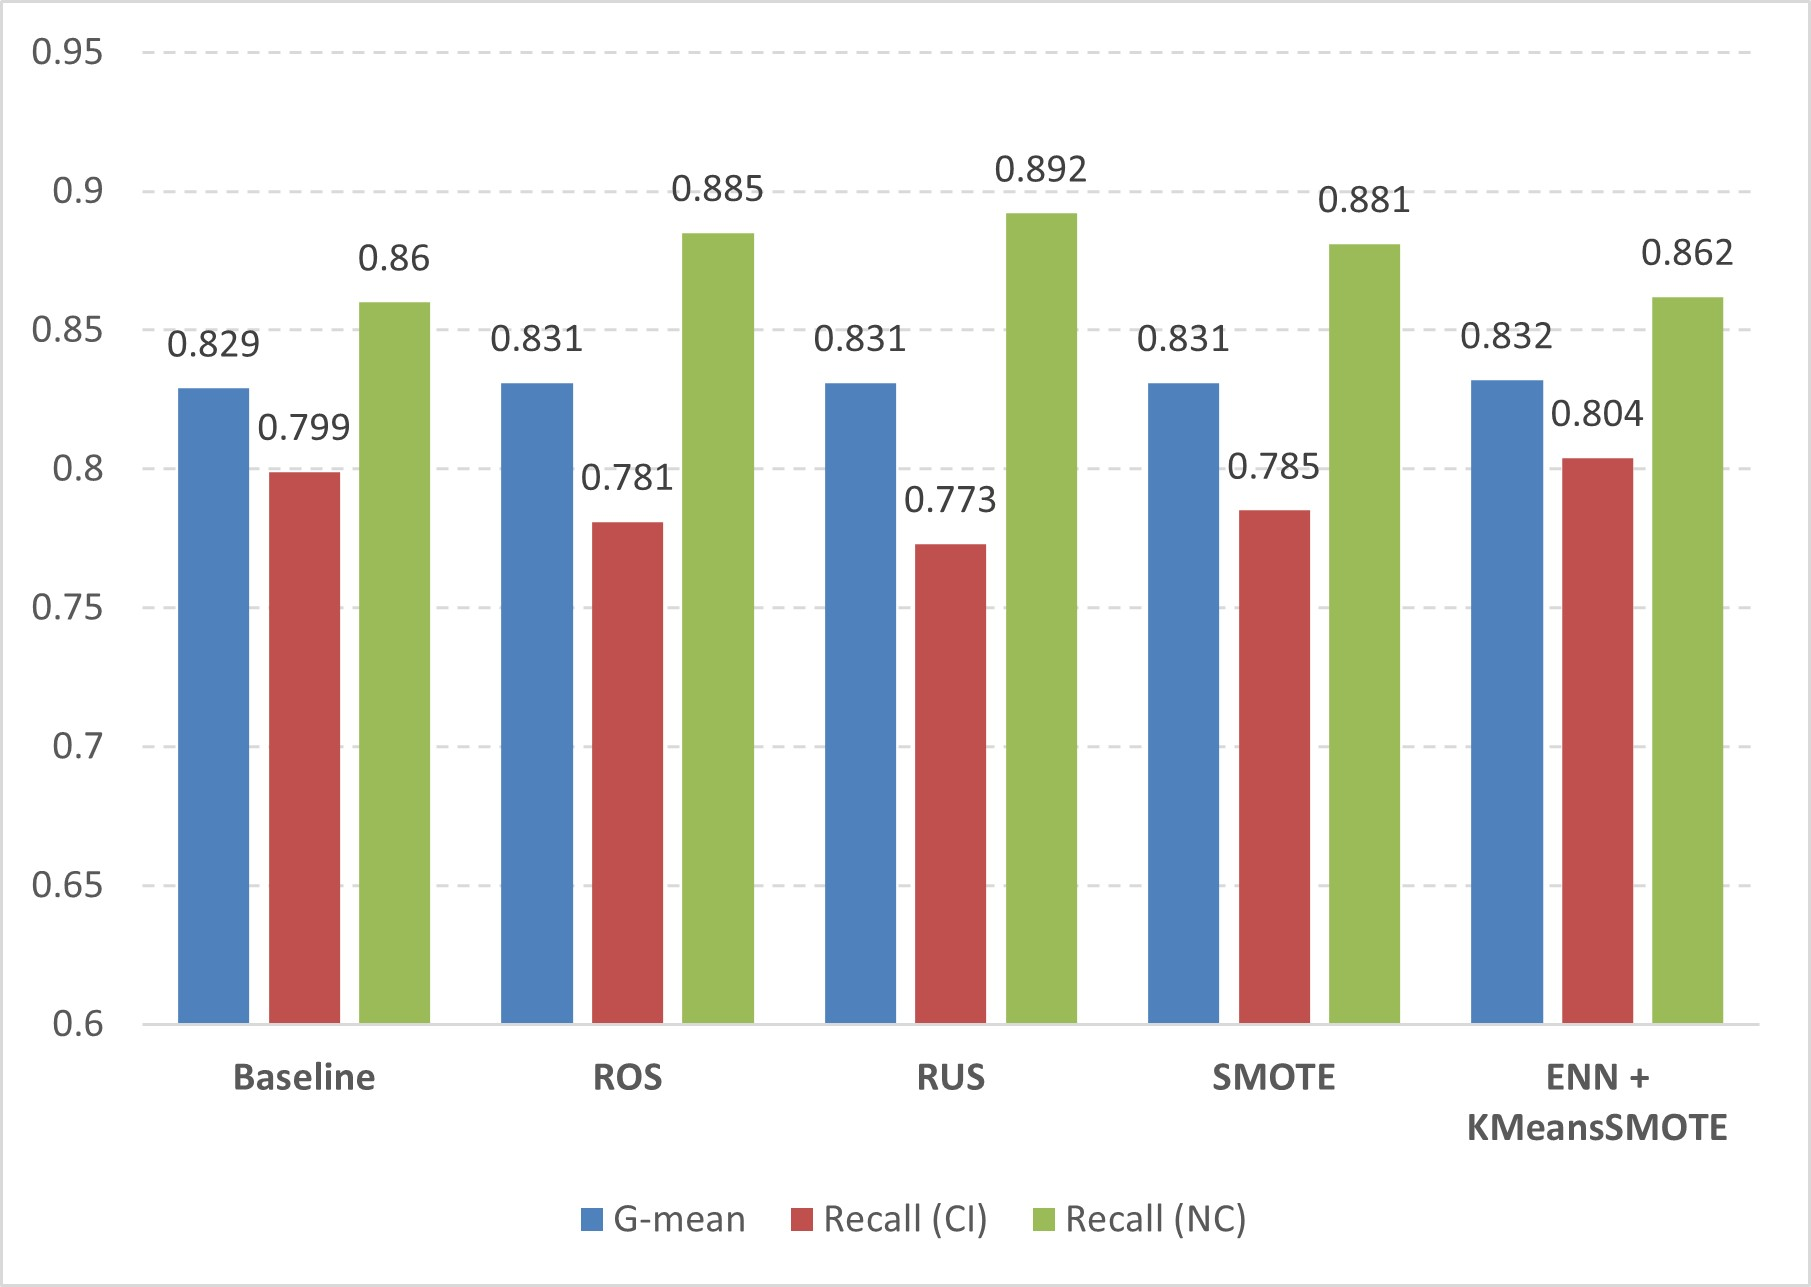
\includegraphics[width=1\textwidth]{figures/data-resampling-task1.jpg}
\caption{Model performance comparison of data resampling methods for the NC vs. CI classification task}
\label{figure:nc_ci_resampling_perf}
\end{figure}

The results show that the baseline model was most affected in its ability to correctly identify the CI class. The baseline RF model achieved a CI recall of only 0.799, although CI is the majority class. The standard resampling methods showed only marginal improvements. Random Oversampling (\acrshort{ROS}) and the Synthetic Minority Over-sampling Technique (\acrshort{SMOTE})  performed similarly. Both methods failed to reduce the high class overlap (N1 of 0.293 and 0.280, respectively) and showed no significant improvement in the CI class recall. Random Undersampling (\acrshort{RUS}) provided a slight reduction in overlap but achieved a G-mean of 0.831 by increasing the recall of the NC class to 0.892 while reducing the recall of the CI class to 0.773.

In contrast, the highest balanced performance (G-mean = 0.832) was achieved using the selected ENN + KMeansSMOTE method. This improvement can be explained by the significant reduction in the class overlap at the instance-level (kDN) to 0.005 and the structural class overlap (N1) to 0.059.  As a result, the recall for the impacted CI class improved to 0.804 while maintaining a high recall for the NC class. \hl{The G-mean improvement of the proposed ENN + KMeansSMOTE method over the baseline was statistically significant (p = 0.026), which confirms that the gain did not occur by random chance.} This confirms the effectiveness of the specialized, overlap-aware strategy.

\subsubsection{Data Resampling Results for the CIND vs. Dementia Classification Task}
\label{sec:resampling_cind_dem}
The baseline characteristics for the CIND vs. dementia task were also analyzed. A low class imbalance was found, with an IR of 1.23. The instance-level class overlap was 0.193 (kDN), and the structural class overlap (N1) was 0.281.

According to the resampling decision algorithm (Algorithm \ref{alg:data-resampling}), data resampling was skipped for this task. This decision was made because the class imbalance was not severe (IR < 2.0) and the instance-level class overlap measures were below the 0.3 threshold. Although a low class imbalance was present, the baseline RF model performance was examined and found to be acceptable in both classes. The baseline model achieved a G-mean of 0.815. It also obtained a recall of 0.807 for the CIND class and 0.824 for the more critical dementia class. This performance was considered a sufficient and balanced starting point for model fine-tuning. Therefore, no resampling methods were applied to this dataset.

In summary, for both classification tasks related to the first research objective, the data complexity was systematically analyzed. The overlap-guided resampling strategy was successfully applied to the NC vs. CI task, creating a more balanced and separable dataset. For the simpler CIND vs. dementia task, the methodology correctly identified that resampling was not necessary. Thus, the original data structure was preserved. This process prepared data for model fine-tuning to achieve the highest possible performance, which is reported in the following subsection.

\subsection{Model Fine-tuning and Selection Results}
After the data resampling step, model fine-tuning and selection were performed. This section shows the results of optimizing and selecting cost-effective models for the two current cognitive status classification tasks. 

\subsubsection{Model Fine-tuning and Selection Results for the NC vs. CI Classification Task} 
The model selection process started by using the cost-effective model selection algorithm (Algorithm \ref{alg:model-selection}) on the grid search hyperparameters fine-tuning results for all five evaluated modeling algorithms. These are k-Nearest Neighbors (\acrshort{KNN}), Logistic Regression (\acrshort{LR}), Light Gradient Boosting Machine (\acrshort{LightGBM}), Random Forest (RF), and Support Vector Machines (\acrshort{SVM}). The goal of the selection algorithm was to find the set of hyperparameter values that produce the most cost-effective model (a model that balances between performance and efficiency). For most classification algorithms (like RF, LR, KNN, and LightGBM), the selection algorithm found a model that was more cost-effective than the best-performing model (the benchmark). This resulted in a considerable efficiency gain, with the highest improvement in training and prediction speed noticed in the LightGBM model. The selection algorithm selected an efficient KNN model with a 1.37 faster prediction speed and the same level of performance as the benchmark model. On the other hand, the algorithm selected the benchmark model for SVM because there was no better alternative. Table~\ref{table:task1_finalists_models} shows a summary of the five finalist fine-tuned models (one model for each algorithm). The table compares their performance and their speed. 

\begin{table}[!ht]
    \centering
    \caption{Summary of fine-tuned models for the NC vs. CI classification task}
    \label{table:task1_finalists_models}
    \newcolumntype{C}{>{\centering\arraybackslash}X}
        \begin{tabularx}{\textwidth}{|C|C|C|C|C|}
        \hline
        \textbf{Model} & 
        \textbf{F1-score (95\% CI)} & 
        \textbf{G-mean (95\% CI)} & 
        \textbf{Training Throughput (Gain)\textsuperscript{1}} & 
        \textbf{Prediction Throughput (Gain)\textsuperscript{1}} \\
        \hline
        KNN & 
        0.844 ($\pm 0.002$) & 
        0.831 ($\pm 0.002$) & 
        $664,626$ $(1.08\times)$ & 
        $12,058$ $(1.37\times)$ \\
        \hline
        LR & 
        0.848 ($\pm 0.002$) & 
        0.842 ($\pm 0.002$) & 
        $1,511,839$ $(1.07\times)$ & 
        $24,641,680$ $(1.09\times)$ \\
        \hline
        LightGBM & 
        0.843 ($\pm 0.002$) & 
        0.837 ($\pm 0.002$) & 
        $227,781$ $(1.28\times)$ & 
        $1,307,402$ $(1.45\times)$ \\
        \hline
        RF & 
        0.849 ($\pm 0.002$) & 
        0.842 ($\pm 0.002$) & 
        $39,407$ $(1.12\times)$ & 
        $263,545$ $(1.21\times)$ \\
        \hline
        SVM & 
        0.848 ($\pm 0.001$) & 
        0.842 ($\pm 0.001$) & 
        $1,721$ & 
        $11,613$ \\
        \hline
        \multicolumn{5}{p{400pt}}{\footnotesize \textsuperscript{1}\hl{Training throughput is reported in training samples per second, and prediction throughput in predictions per second.} Gain is calculated as the ratio of the selected model’s throughput to the benchmark model’s throughput. Values indicate the factor by which training and prediction speed have improved. Gain is not presented when the selected model is the benchmark model.}
    \end{tabularx}
\end{table}

Another assessment was done to choose the best model for this classification task. The five models were assessed based on three main criteria: performance, efficiency (the model's training and prediction speed), and interpretability (how easy it is to explain the model's prediction). From the results in Table~\ref{table:task1_finalists_models}, the LR model was selected as the final model for this classification task.

This choice was made for several reasons. First, LR was one of the models with the highest performance. It achieved an F1-score of 0.848 and a G-mean of 0.842. This performance is very close to the performance of the RF and SVM models. These two models obtained F1-scores of 0.849 and 0.848, respectively. Other models (KNN and LightGBM) had slightly lower performance, so they were not selected. Second, when comparing the top three models (LR, RF, and SVM), their efficiency was the main difference. The LR model was substantially faster than all the other models. The LR model was extremely faster than the SVM model, which had the slowest training and prediction speed among the three best-performing models. Finally, one of the objectives of this study is to develop models that are easy to explain. The coefficients of the LR model can be directly inspected to understand how each feature contributes to the classification. This gives it a clear advantage over the complex and ensemble models like non-linear SVM, RF, and LightGBM models. In the end, the RF and SVM models had a high performance, but they were not the most efficient and interpretable models. LR was the only model that offered the best balance of good performance, great speed, and simple interpretation. Table~\ref{table:lr-fine-tune-task1-apdx} in the appendix presents the hyperparameter fine-tuning results of the LR model.

\subsubsection{Model Fine-tuning and Selection Results for the CIND vs. Dementia Classification Task}
The same process of model fine-tuning and selection was applied to the CIND vs. dementia classification task. The proposed selection algorithm was also used to identify models that optimize the trade-off between accuracy and computational cost. More efficient RF, LightGBM, and KNN models were successfully identified by the selection algorithm. The RF model speed improved by approximately two-times with very minimal decrease in performance. On the other hand, the LR best-performing model was also the most efficient model among the other LR optimized models. Therefore, the best-performing model was retained by the selection algorithm. The performance and throughput of the five fine-tuned models are presented in Table~\ref{table:task2_finalists_models}.

\begin{table}[!ht]
\centering
\caption{Summary of fine-tuned models for the CIND vs. dementia classification task}
\label{table:task2_finalists_models}
\newcolumntype{C}{>{\centering\arraybackslash}X}
    \begin{tabularx}{\textwidth}{|C|C|C|C|C|}
    \hline
    \textbf{Model} &
    \textbf{F1-score (95\% CI)} &
    \textbf{G-mean (95\% CI)} &
    \textbf{Training Throughput (Gain)\textsuperscript{1}} &
    \textbf{Prediction Throughput (Gain)\textsuperscript{1}} \\
        \hline
        KNN &
        0.814 ($\pm 0.004$) &
        0.800 ($\pm 0.003$) &
        $713,015$ $(1.08\times)$ &
        $16,084$ $(2.14\times)$ \\
        \hline
        LR &
        0.842 ($\pm 0.006$) &
        0.828 ($\pm 0.007$) &
        $512,085$ &
        $19,831,465$ \\
        \hline
        LightGBM &
        0.844 ($\pm 0.006$) &
        0.825 ($\pm 0.008$) &
        $146,969$ $(1.24\times)$ &
        $686,674$ $(1.20\times)$ \\
        \hline
        RF &
        0.844 ($\pm 0.005$) &
        0.830 ($\pm 0.006$) &
        $30,959$ $(2.01\times)$ &
        $146,642$ $(2.02\times)$ \\
        \hline
        SVM &
        0.843 ($\pm 0.006$) &
        0.831 ($\pm 0.006$) &
        $531$ $(1.07\times)$ &
        $3,526$ $(1.00\times)$ \\
        \hline
        \multicolumn{5}{p{400pt}}{\footnotesize \textsuperscript{1}\hl{Training throughput is reported in training samples per second, and prediction throughput in predictions per second.} Gain is calculated as the ratio of the selected model’s throughput to the benchmark model’s throughput. Values indicate the factor by which training and prediction speed have improved. Gain is not presented when the selected model is the benchmark model.}
    \end{tabularx}
\end{table}

To determine the optimal model for this specific classification task, a comprehensive assessment was conducted. This is done by evaluating the five optimized models based on performance, efficiency, and interpretability. From these criteria, the LR model was identified as the most suitable cost-effective choice. Regarding performance, a highly competitive group of models was observed. An F1-score of 0.842 was obtained by the LR model. This score is statistically comparable to the RF (0.844), LightGBM (0.844), and SVM (0.843) models. On the other hand, a low F1-score of 0.814 was observed in the KNN model, so it was excluded from the final selection. Because a very similar performance was achieved by the top four models, the final decision was based on computational efficiency. A high speed in training and prediction was demonstrated by the LR model, with a prediction throughput exceeding 19 million samples per second.  This is much faster than LightGBM, RF, and SVM. Furthermore, high interpretability is ensured by the linear nature of the LR model. This is different from the complex structures of ensemble and non-linear models. Consequently, the LR model was selected; although slightly higher accuracy was offered by RF and SVM, they lacked the balance of efficiency and explainability that are needed for this study. The hyperparameter fine-tuning results of the LR model is presented in Table~\ref{table:lr-fine-tune-task2-apdx} in the appendix.

In conclusion, the model fine-tuning and selection process identified the LR model as the suitable cost-effective model for both the NC vs. CI and CIND vs. dementia classification tasks. By selecting a model that is both highly efficient and easy to interpret while maintaining competitive performance, the study successfully addresses the requirements of the first research objective. Finally, the robustness and generalizability of these selected LR models are further assessed in the next section.

\subsection{Model Performance in External Validation}
\label{sec:classification_external_validation}
The generalizability of the selected LR models was assessed for the two current cognitive status classification tasks. This was done by evaluating their performance and clinical utility in the NACC cross-center testing dataset and the independent Alzheimer's Disease Neuroimaging Initiative (\acrshort{ADNI}) dataset. A detailed description of the validation methodology is provided in section \ref{sec:model-validation}.

\subsubsection{External Validation Results for the NC vs. CI Classification Task}
The performance of the LR model in internal and external validations for the NC vs. CI classification task was analyzed. A summary of the performance metrics is presented in Table~\ref{table:nc_ci_results}. Additionally, the Receiver Operating Characteristic (\acrshort{ROC}) curves for the three validation stages are illustrated in Figure~\ref{figure:nc_ci_roc}.

\begin{table}[!ht]
    \centering
    \caption{Performance of the selected logistic regression model in internal and external validation for the NC vs. CI classification task}
    \label{table:nc_ci_results}
    \newcolumntype{C}{>{\centering\arraybackslash}X}
        \begin{tabularx}{\textwidth}{|c|c|C|C|}
            \hline
            \textbf{Metric} & \textbf{Internal CV} & \textbf{NACC Cross-center Validation} & \textbf{ADNI External Validation} \\
            \hline
            AUC & \makecell{0.844 \\ {\small \hl{(0.843--0.846)}}} & \makecell{0.810 \\ {\small \hl{(0.802--0.818)}}} & \makecell{0.825 \\ {\small \hl{(0.807--0.842)}}} \\ \hline
            G-mean & 0.842 & 0.809 & 0.820 \\ \hline
            Sensitivity & 0.785 & 0.777 & 0.739 \\ \hline
            Specificity & 0.903 & 0.843 & 0.911 \\ \hline
            F1-score & 0.848 & 0.823 & 0.833 \\
            \hline
            \multicolumn{4}{p{400pt}}{\footnotesize \hl{AUC: area under the curve, F1-score: harmonic mean of precision and recall, G-mean: geometric mean score, Sensitivity: recall of the CI class, Specificity: recall of the NC class.}}
        \end{tabularx}
\end{table}

\begin{figure}[ht]
    \centering
    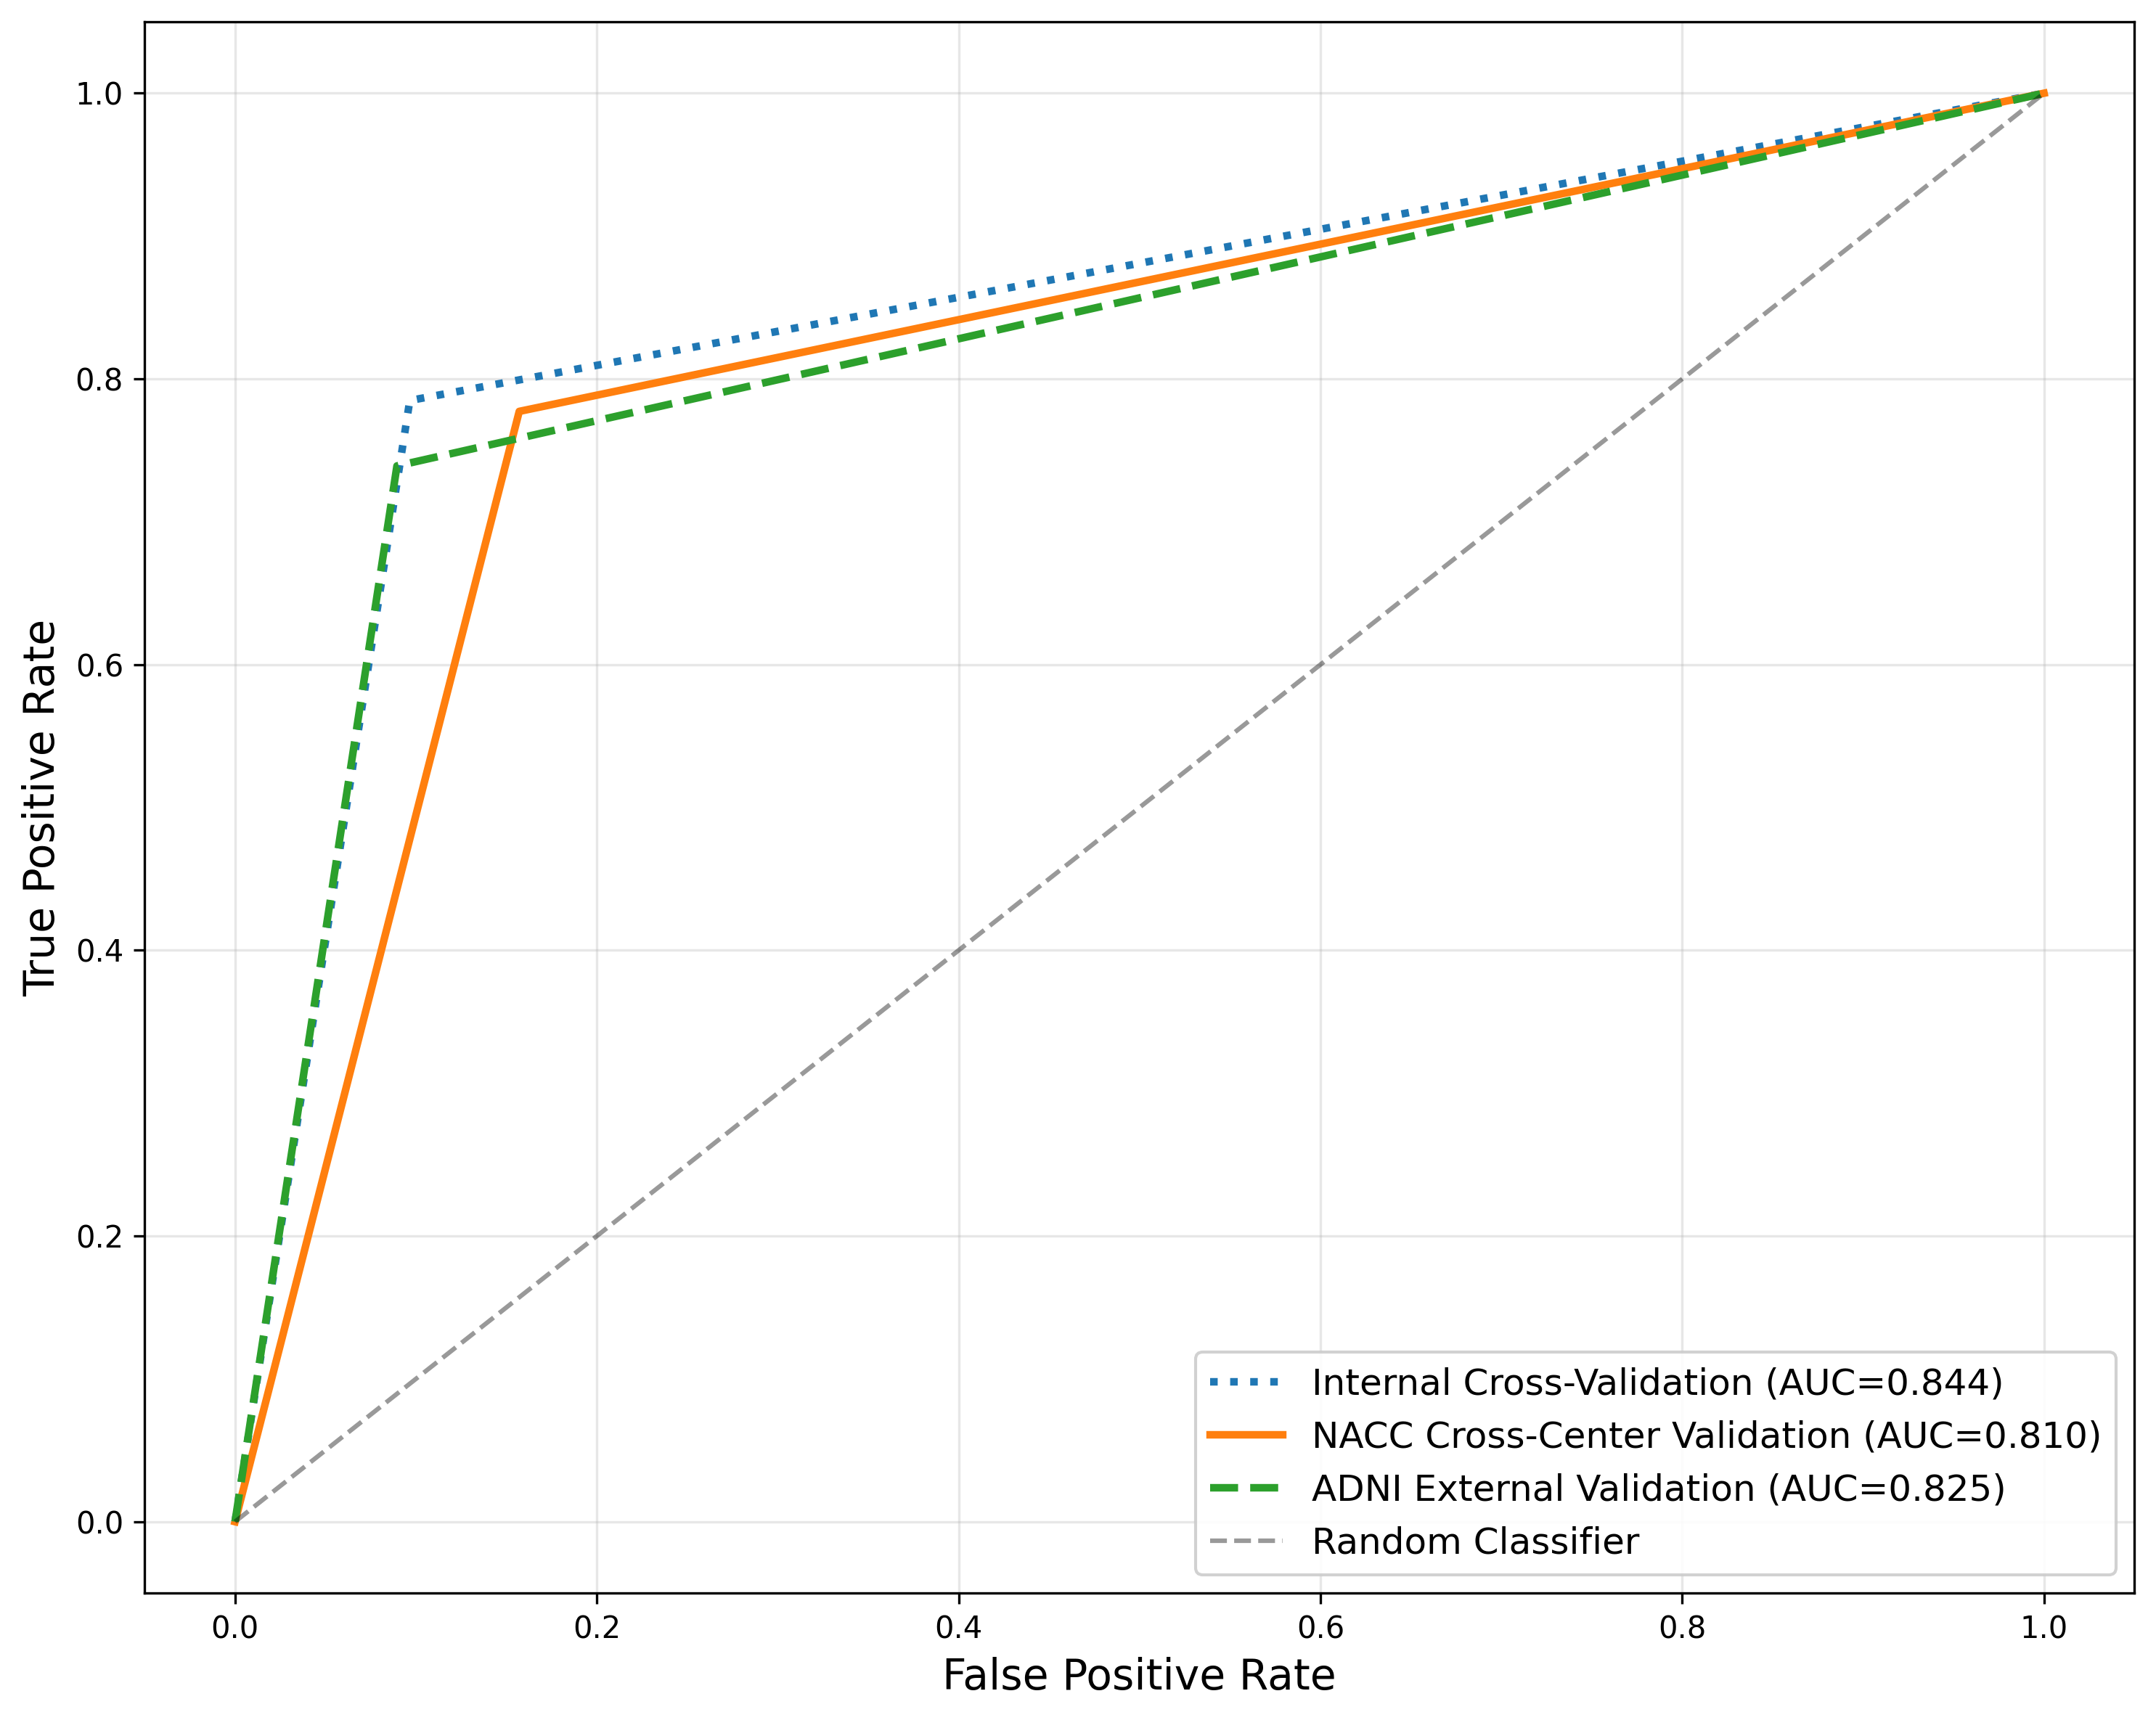
\includegraphics[width=0.7\textwidth]{figures/impaired_classification_all_tests_roc_overlay.png}
    \caption{ROC curves comparing the performance of the logistic regression model for the NC vs. CI classification task}
    \begin{minipage}{\textwidth}
      \footnotesize \hl{The horizontal axis shows the false positive rate (1 -- specificity) and the vertical axis shows the true positive rate (sensitivity). Each curve represents one validation dataset.}
    \end{minipage}
    \label{figure:nc_ci_roc}
\end{figure}

Based on the results of testing the LR model with the NACC cross-center testing dataset, a moderate decrease in overall performance was noticed. A drop of 0.034 in the area under the curve (\acrshort{AUC}) score was recorded, which decreased from 0.844 in the internal cross-validation (CV) to 0.810 in the NACC cross-center validation. A similar decrease was noticed in the G-mean. This performance reduction is due to the major drop in NC recall (specificity) from 0.903 to 0.843, although CI recall (sensitivity) had a minor decrease. The LR struggled to accurately classify NC in the NACC cross-center testing data, compared to the internal CV and the ADNI data. 

Regarding generalizability to the independent ADNI dataset, the LR model achieved high performance, with an AUC score of 0.825. This score is slightly higher than the score of 0.810 in the NACC cross-center validation. The ROC curves in Figure~\ref{figure:nc_ci_roc} demonstrate the performance of the LR in different validations. A notable trade-off between sensitivity and specificity was observed in the ADNI results. Despite a high specificity (0.911), the model's sensitivity score dropped to 0.739, which is a significantly lower score than the score obtained in the NACC cross-center validation. This is likely due to differences in characteristics between the observational NACC study and the ADNI clinical trial. Although high overall accuracy was maintained (as shown by an F1-score of 0.833), the low sensitivity indicates that the LR model is not accurate in classifying CI cases compared to NC cases when used on the ADNI external data. \hl{The reduction in AUC from the internal CV was statistically significant for both the NACC cross-center (p < 0.001) and ADNI (p < 0.001) validations although it should be noted that the very low variance across the five CV folds (SD = 0.002) makes the test highly sensitive to even minor performance differences.} The external validation results are reported with extended performance metrics in Table~\ref{table:lr-complete-perf-task1-apdx} in the appendix.

The prediction of the LR model was calibrated to ensure that it generates probabilities that reflect the actual risk of CI. The results of the model calibration in the two external validation datasets are presented in Figure~\ref{fig:nc_ci_calib_curve}. In the NACC cross-center validation, the uncalibrated LR model tended to overestimate the risk of CI in most probability thresholds (intercept = -0.235). In addition, a slope of 0.191 indicates that the model produced extreme estimations close to 0 and 1. After beta calibration was applied, the model's prediction improved across all probability levels. In general, the Expected Calibration Error (\acrshort{ECE}) decreased significantly from 0.151 to 0.027, and the Brier score improved from 0.168 to 0.136. This indicates that the model's predicted probabilities of CI became closer to the true outcome rates. A different result was observed in the ADNI external validation. In this test, the model underestimated the risk of CI even after applying the beta calibration, which reduced the calibration error from 0.176 to 0.107.

\begin{figure}[ht]
    \centering
    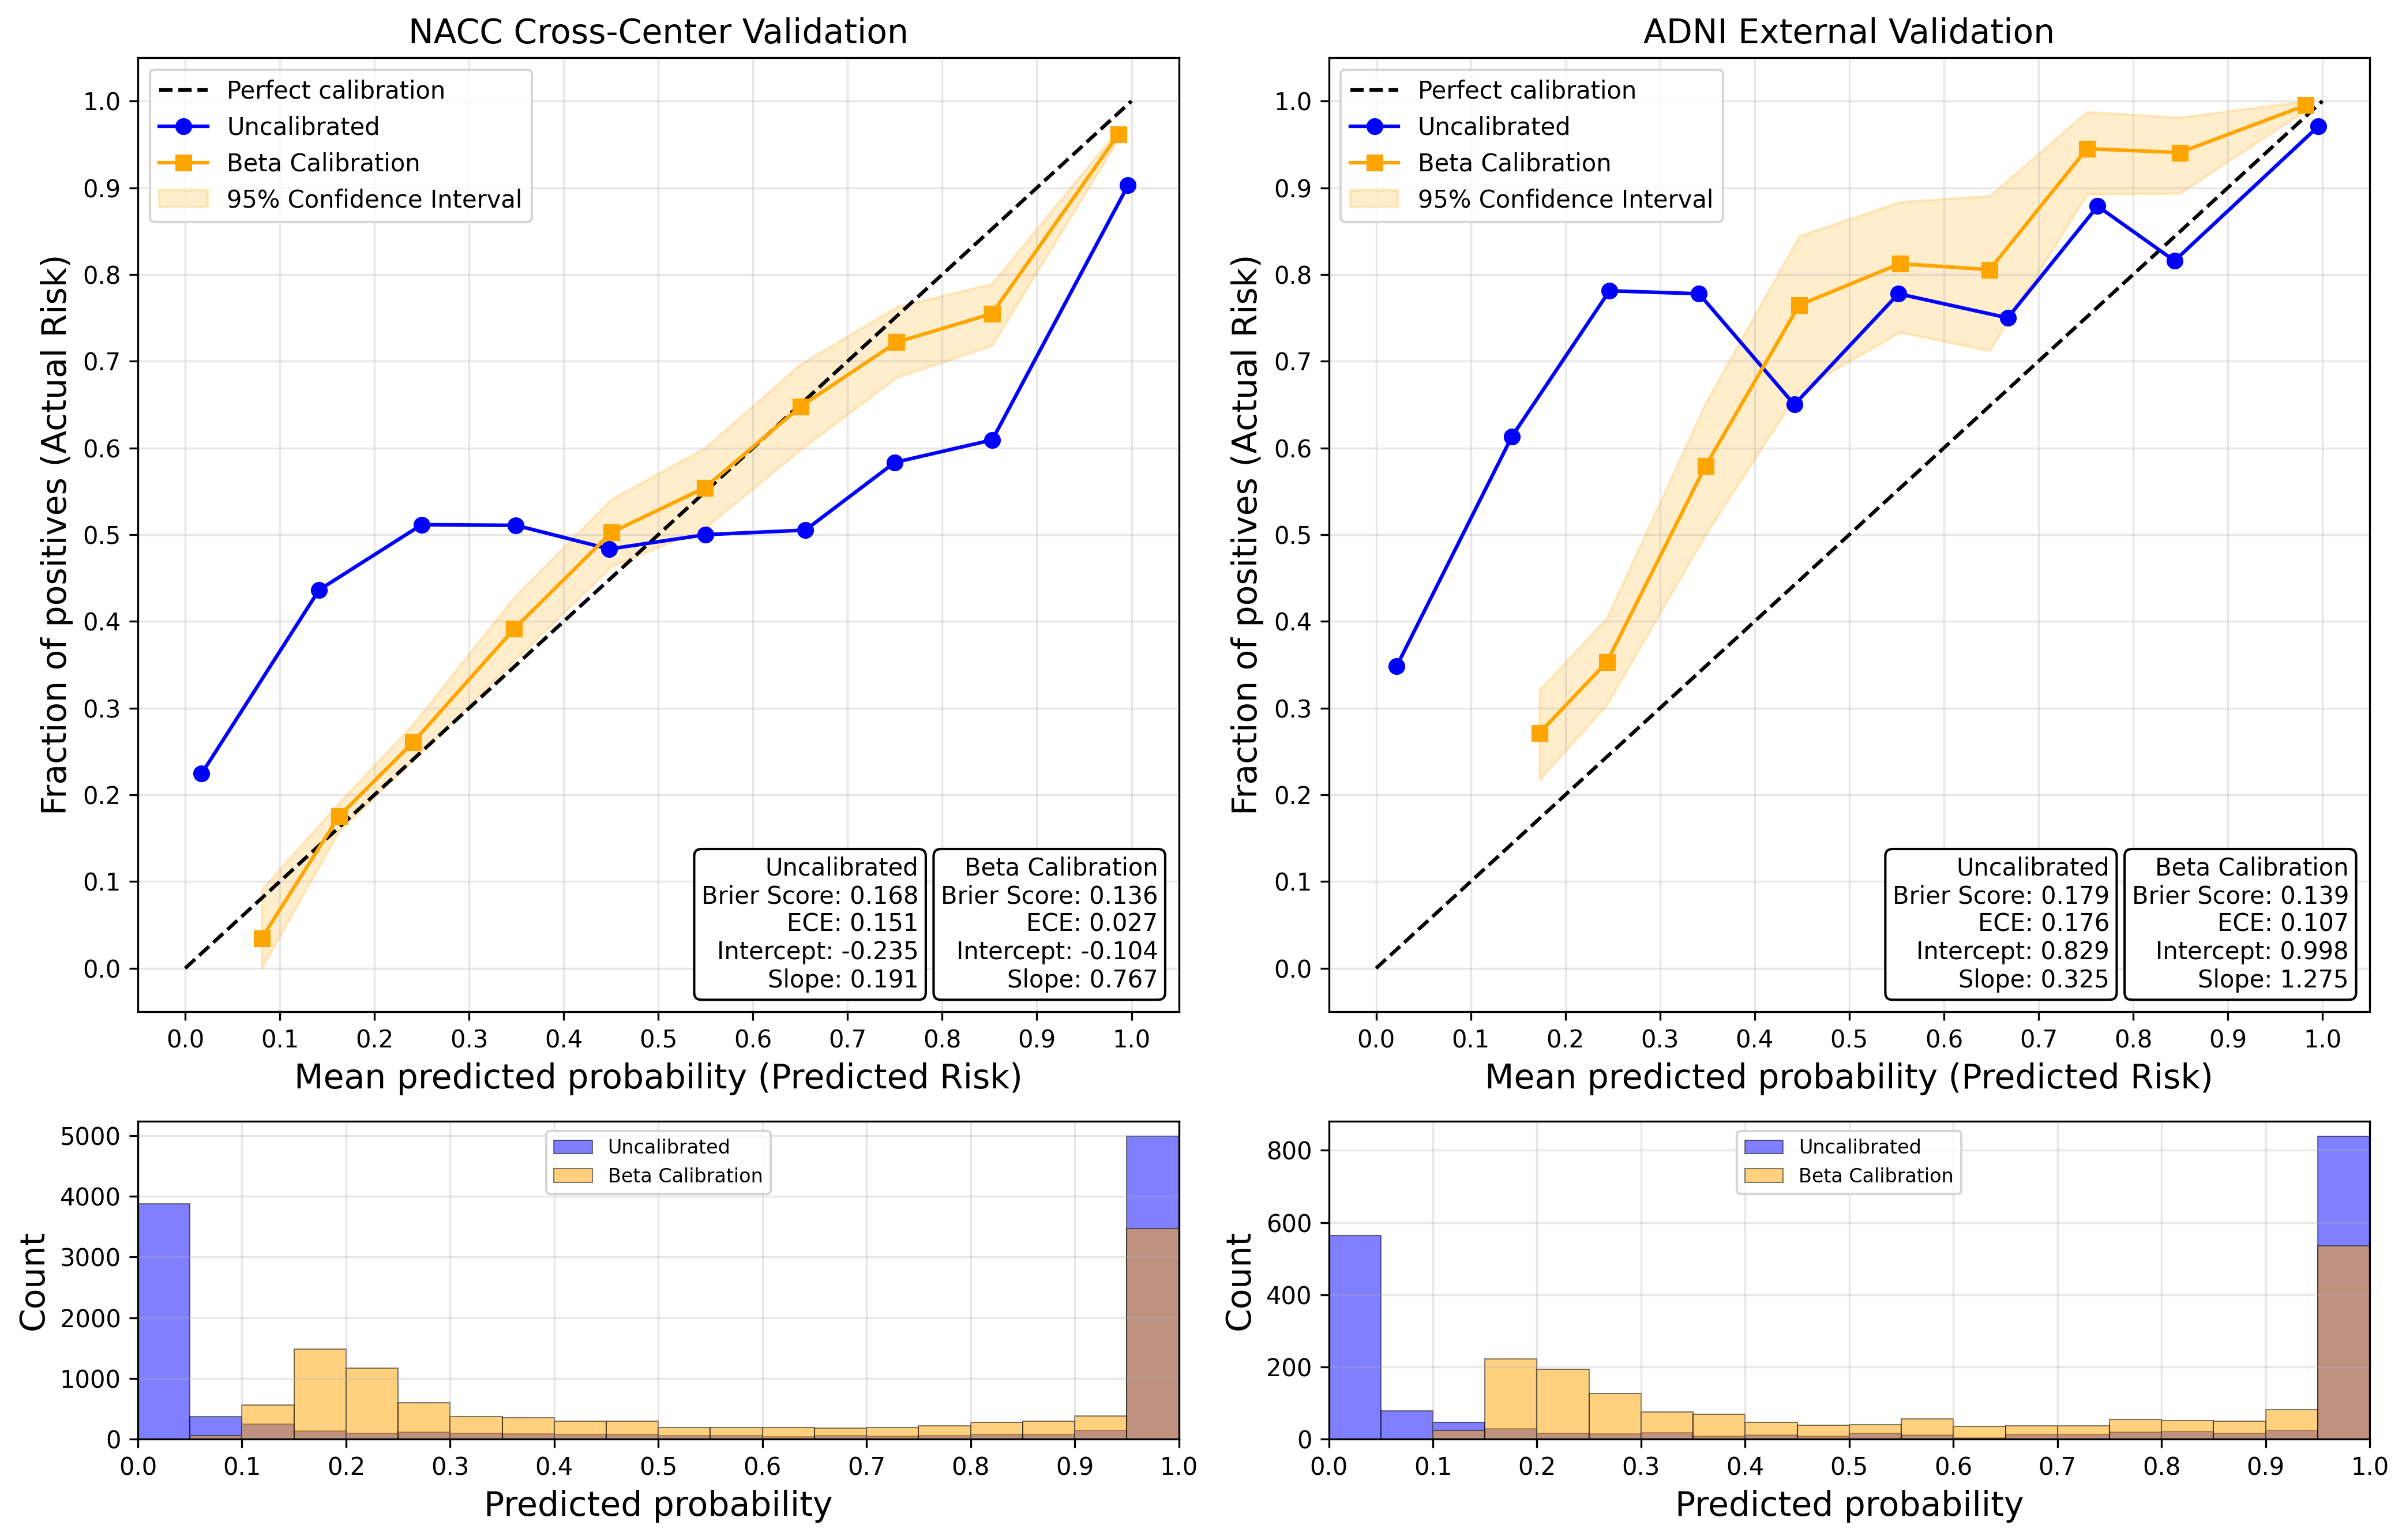
\includegraphics[width=1.0\textwidth]{figures/calibration/impaired_classification_both_calibration_curve.png}
    \caption{Model calibration curves for the NC vs. CI classification task}
    \begin{minipage}{\textwidth}
      \footnotesize \hl{The horizontal axis shows the predicted probability and the vertical axis shows the observed frequency of the positive class. The diagonal line represents perfect calibration, and the curves compare the model before and after beta calibration.}
    \end{minipage}
    \label{fig:nc_ci_calib_curve}
\end{figure}

The calibration of the model prediction supported the clinical utility of the calibrated LR model. According to the Decision Curve Analysis (\acrshort{DCA}) presented in Figure~\ref{fig:nc_ci_dca} the model demonstrated a higher net benefit in probability thresholds ranging from 0.16 to 0.98 in the NACC cross-center validation. This shows that the model has strong clinical utility, outperforming "treat all" and "treat none" strategies for almost any risk cutoff.

\begin{figure}[ht]
    \centering
    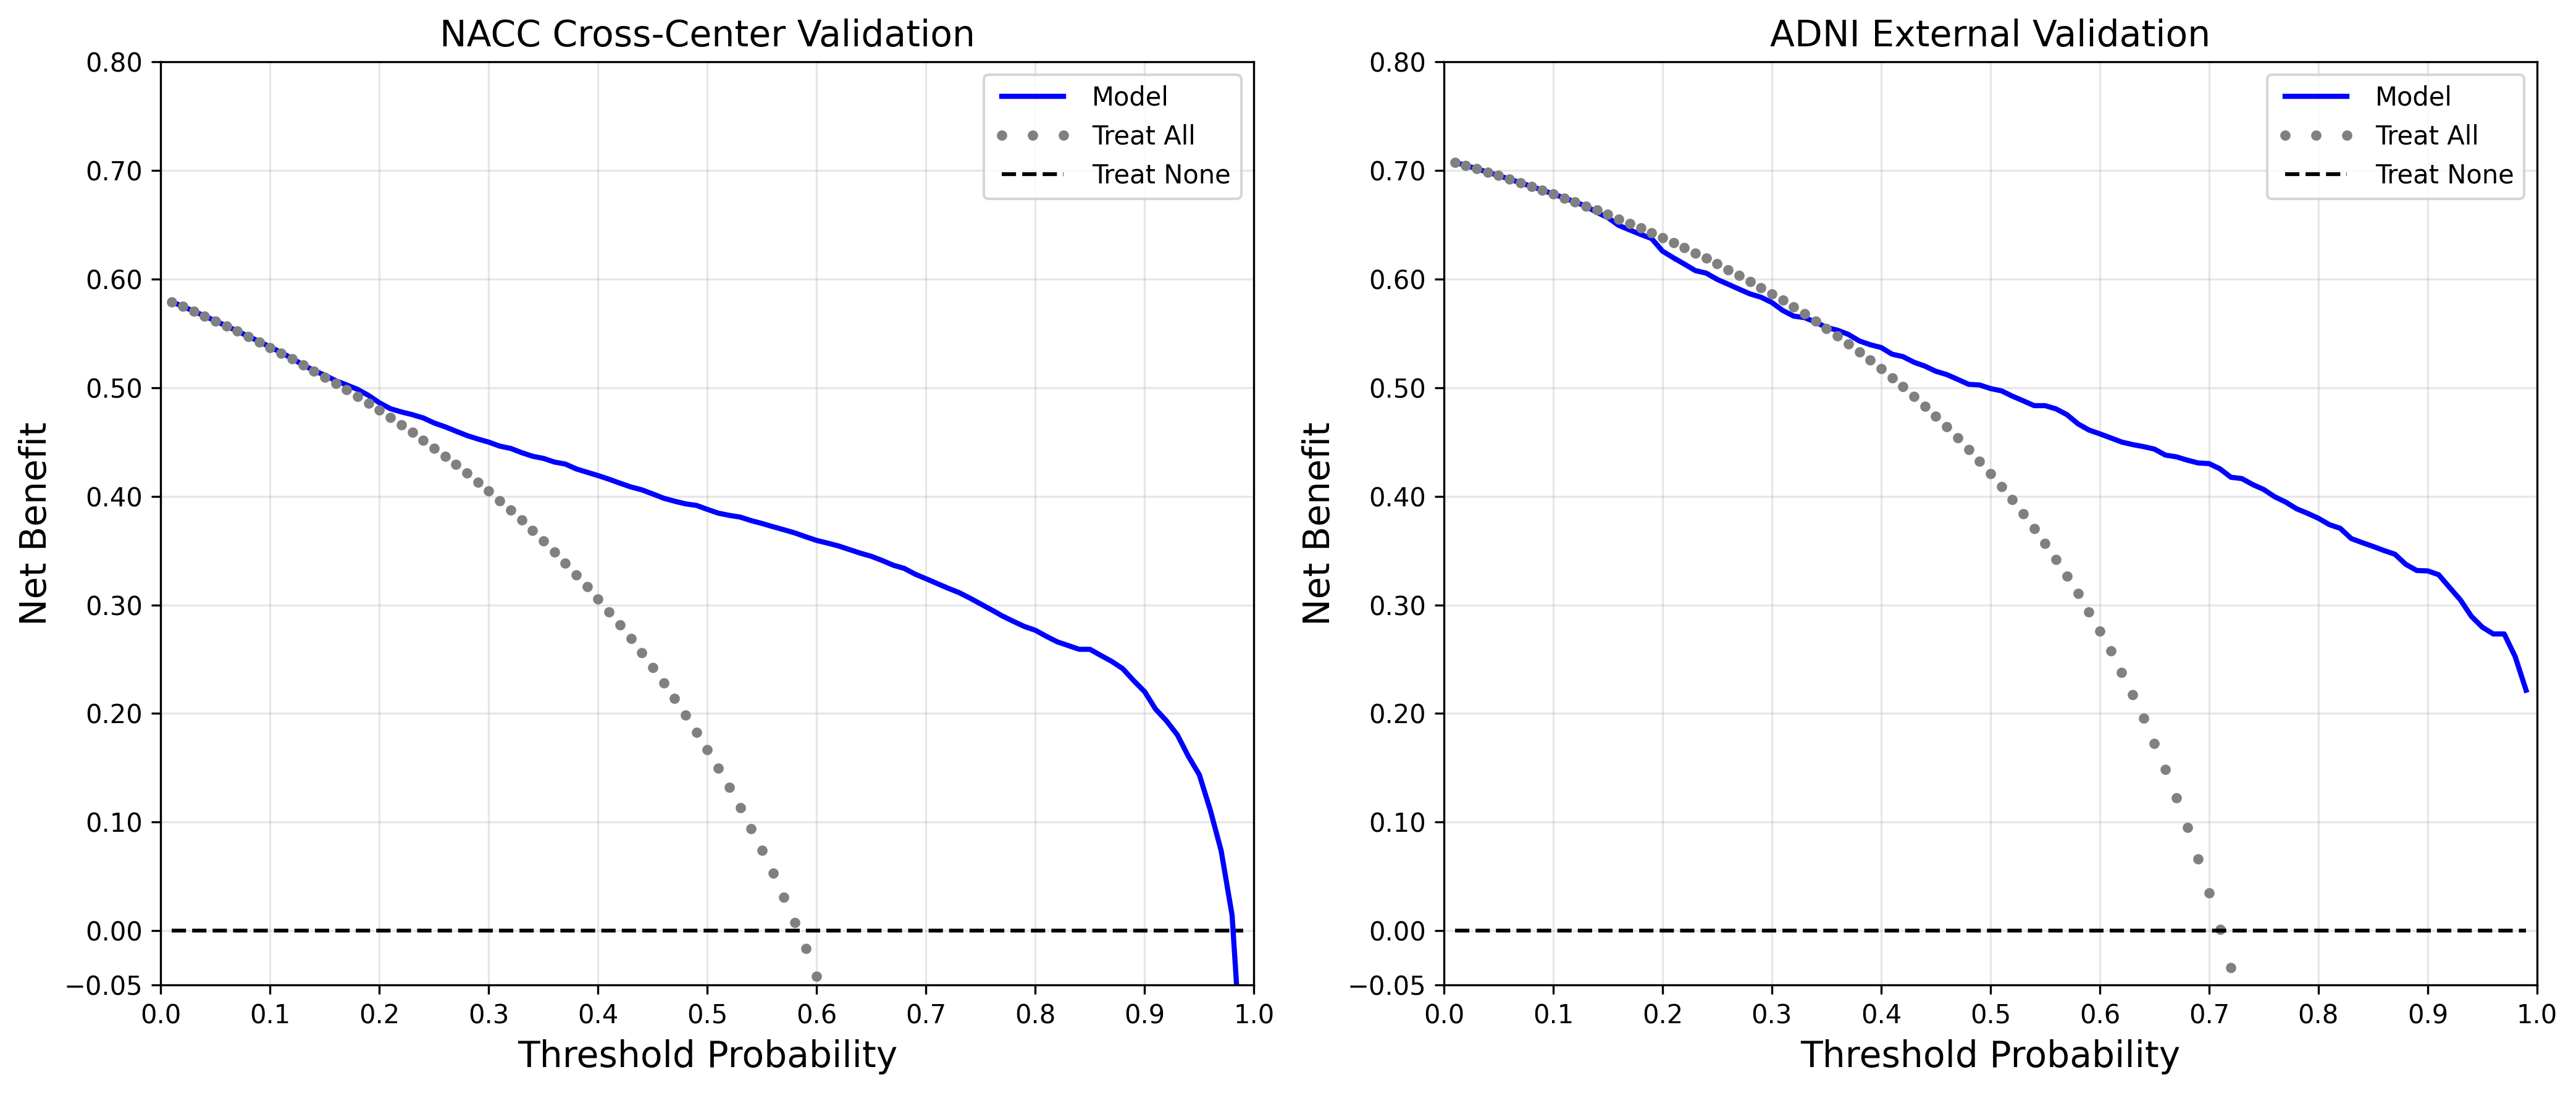
\includegraphics[width=1.0\textwidth]{figures/DCA/impaired_classification_dca_both.png}
    \caption{The decision curve analysis (DCA) for the NC vs. CI classification task}
    \begin{minipage}{\textwidth}
      \footnotesize This figure illustrates the DCA curves of the NACC cross-center validation (left side) and the ADNI external validation (right side). "Treat All" refers to the assumption that all subjects are predicted to have CI, and "Treat None" refers to the assumption that none of the subjects are predicted to have CI.
    \end{minipage}
    \label{fig:nc_ci_dca}
\end{figure}

The clinical utility of the model was limited to thresholds between 0.35 and 0.99 in the ADNI external validation. The model could not identify low-risk subjects and provided no additional benefit compared to the "treat all" strategy at thresholds below 0.35. This could be related to model miscalibration in low probability thresholds observed in the calibration curve in Figure~\ref{fig:nc_ci_calib_curve}.

\subsubsection{External Validation Results for the CIND vs. Dementia Classification Task}
The selected LR model for the CIND vs. dementia classification task was also evaluated to check its performance on unseen data. The results of the internal cross-validation, the NACC cross-center validation, and the ADNI external validation are compared in Table~\ref{table:cind_dementia_results}. The ROC curves for these tests are also presented in Figure~\ref{figure:cind_dementia_roc}.

\begin{table}[!ht]
    \centering
    \caption{Performance of the selected logistic regression model in internal and external validation for the CIND vs. dementia classification task}
    \label{table:cind_dementia_results}
    \newcolumntype{C}{>{\centering\arraybackslash}X}
        \begin{tabularx}{\textwidth}{|c|c|C|C|}
            \hline
            \textbf{Metric} & \textbf{Internal CV} & \textbf{NACC Cross-center Validation} & \textbf{ADNI External Validation} \\
            \hline
            AUC & \makecell{0.828 \\ {\small \hl{(0.821--0.835)}}} & \makecell{0.828 \\ {\small \hl{(0.819--0.837)}}} & \makecell{0.841 \\ {\small \hl{(0.822--0.861)}}} \\ \hline
            G-mean & 0.828 & 0.826 & 0.840 \\ \hline
            Sensitivity & 0.827 & 0.874 & 0.888 \\ \hline
            Specificity & 0.830 & 0.782 & 0.794 \\ \hline
            F1-score & 0.842 & 0.837 & 0.777 \\
            \hline
            \multicolumn{4}{p{400pt}}{\footnotesize \hl{AUC: area under the curve, F1-score: harmonic mean of precision and recall, G-mean: geometric mean score, Sensitivity: recall of the dementia class, Specificity: recall of the CIND class.}}
        \end{tabularx}
\end{table}

\begin{figure}[ht]
    \centering
    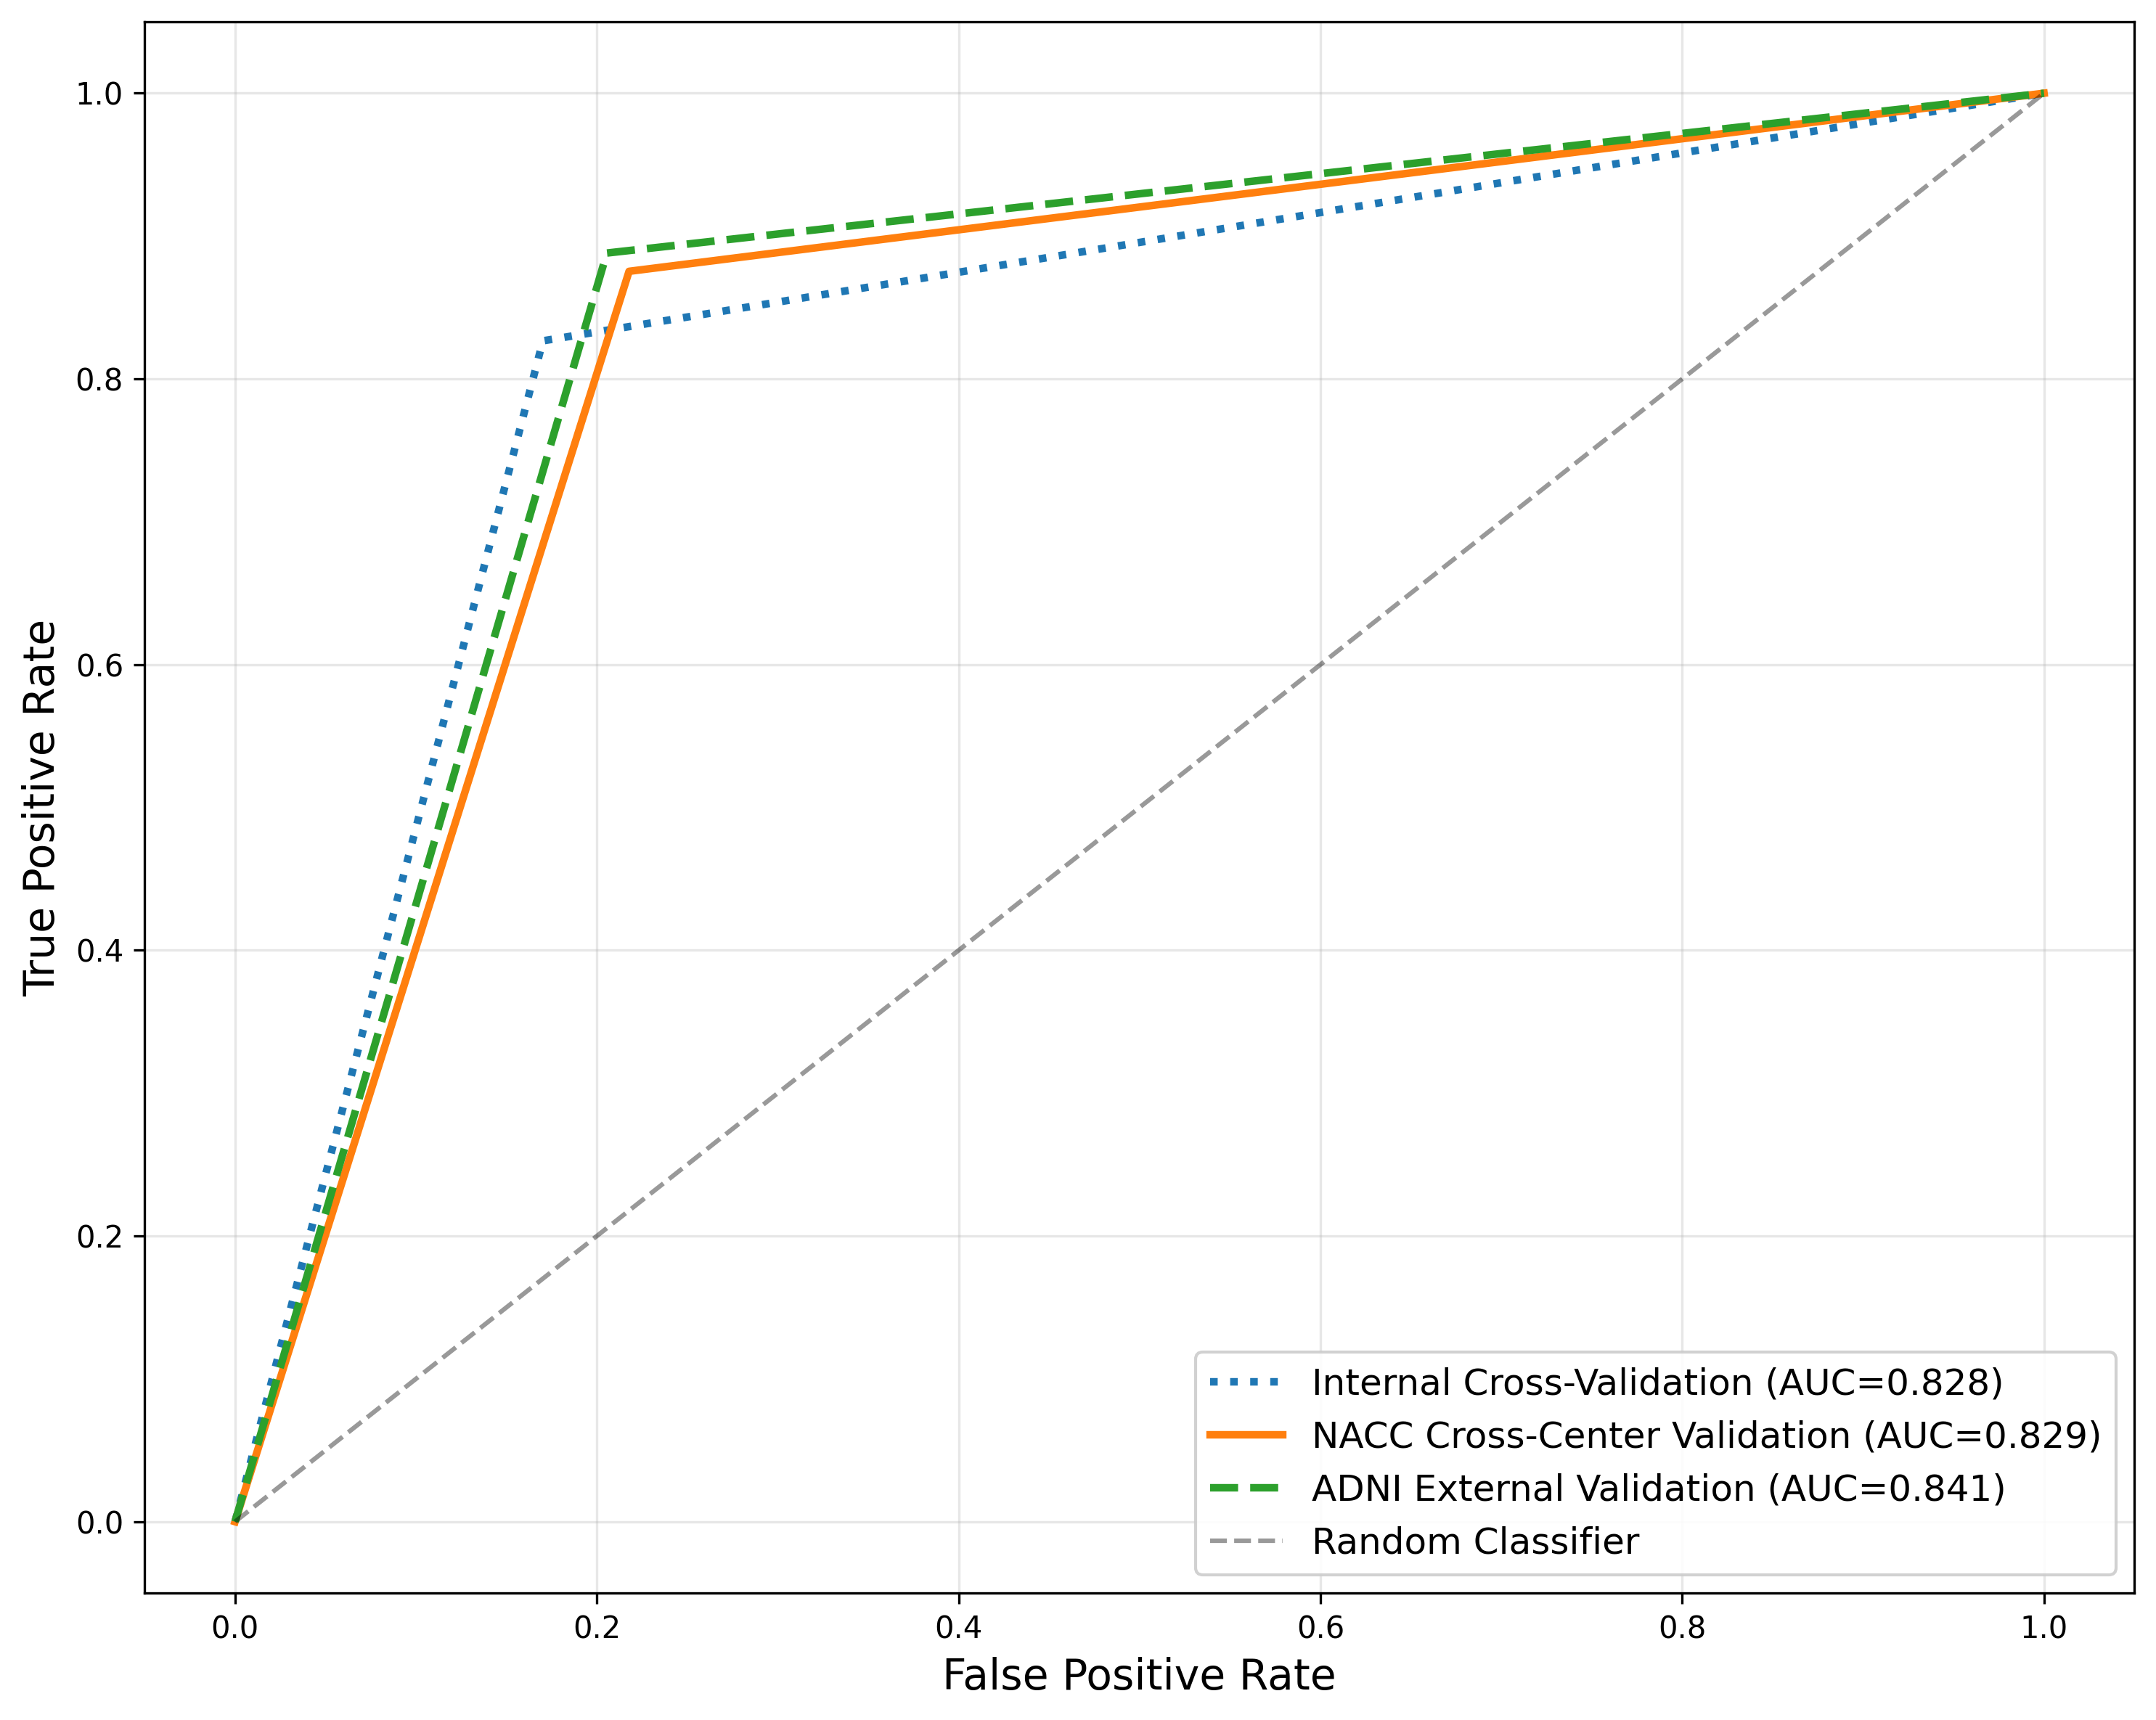
\includegraphics[width=0.7\textwidth]{figures/dementia_classification_all_tests_roc_overlay.png}
    \caption{ROC curves comparing the performance of the logistic regression model for the CIND vs. dementia classification task}
    \begin{minipage}{\textwidth}
      \footnotesize \hl{The horizontal axis shows the false positive rate (1 -- specificity) and the vertical axis shows the true positive rate (sensitivity). Each curve represents one validation dataset.}
    \end{minipage}
    \label{figure:cind_dementia_roc}
\end{figure}

The performance of the LR model on the unseen NACC data was observed to achieve the same AUC as the internal CV and a slight decrease in the G-mean score from 0.828 to 0.826. Additionally, the sensitivity on the NACC cross-center validation increased to 0.874, while the specificity decreased to 0.782. These results indicate that the model correctly classified a high proportion of dementia cases but with a higher false positive rate, which decreased the CIND recall.

The results of the ADNI external validation confirmed that the model is generalizable to different clinical settings. A high AUC of 0.841 was achieved, which exceeded the results of the internal CV and the NACC cross-center validation. This robustness is clearly shown in Figure~\ref{figure:cind_dementia_roc}, where the ADNI curve closely follows or exceeds the other ROC curves. This is a result of a high sensitivity of 0.888, which indicates that the model is highly effective in detecting dementia even in unseen external data. The LR model produced higher precision in classifying both classes (CIND and dementia) in the ADNI external validation compared to the NACC cross-center validation, which can be observed by the G-mean score of 0.840. \hl{The AUC difference between the internal CV and the NACC cross-center validation was not statistically significant (p = 0.912), which supports the close agreement between them, while the higher ADNI AUC was found to be significant (p = 0.038).} Table~\ref{table:lr-complete-perf-task2-apdx} in the appendix provides extended performance metrics of the external validation results.

To ensure that the LR model generates probabilities that accurately reflect the actual risk of dementia, model calibration was performed. The results for both validation datasets are illustrated in Figure~\ref{fig:cind_dementia_calib_curve}. In the NACC cross-center validation, the uncalibrated model already demonstrated strong alignment with the true outcomes. The slope was very close to 1, but the model overestimated the risk of dementia (intercept = -0.461). No improvement was observed after beta calibration because the initial model was already well-calibrated, with an ECE of 0.057 and a Brier score of 0.125.

\begin{figure}[ht]
    \centering
    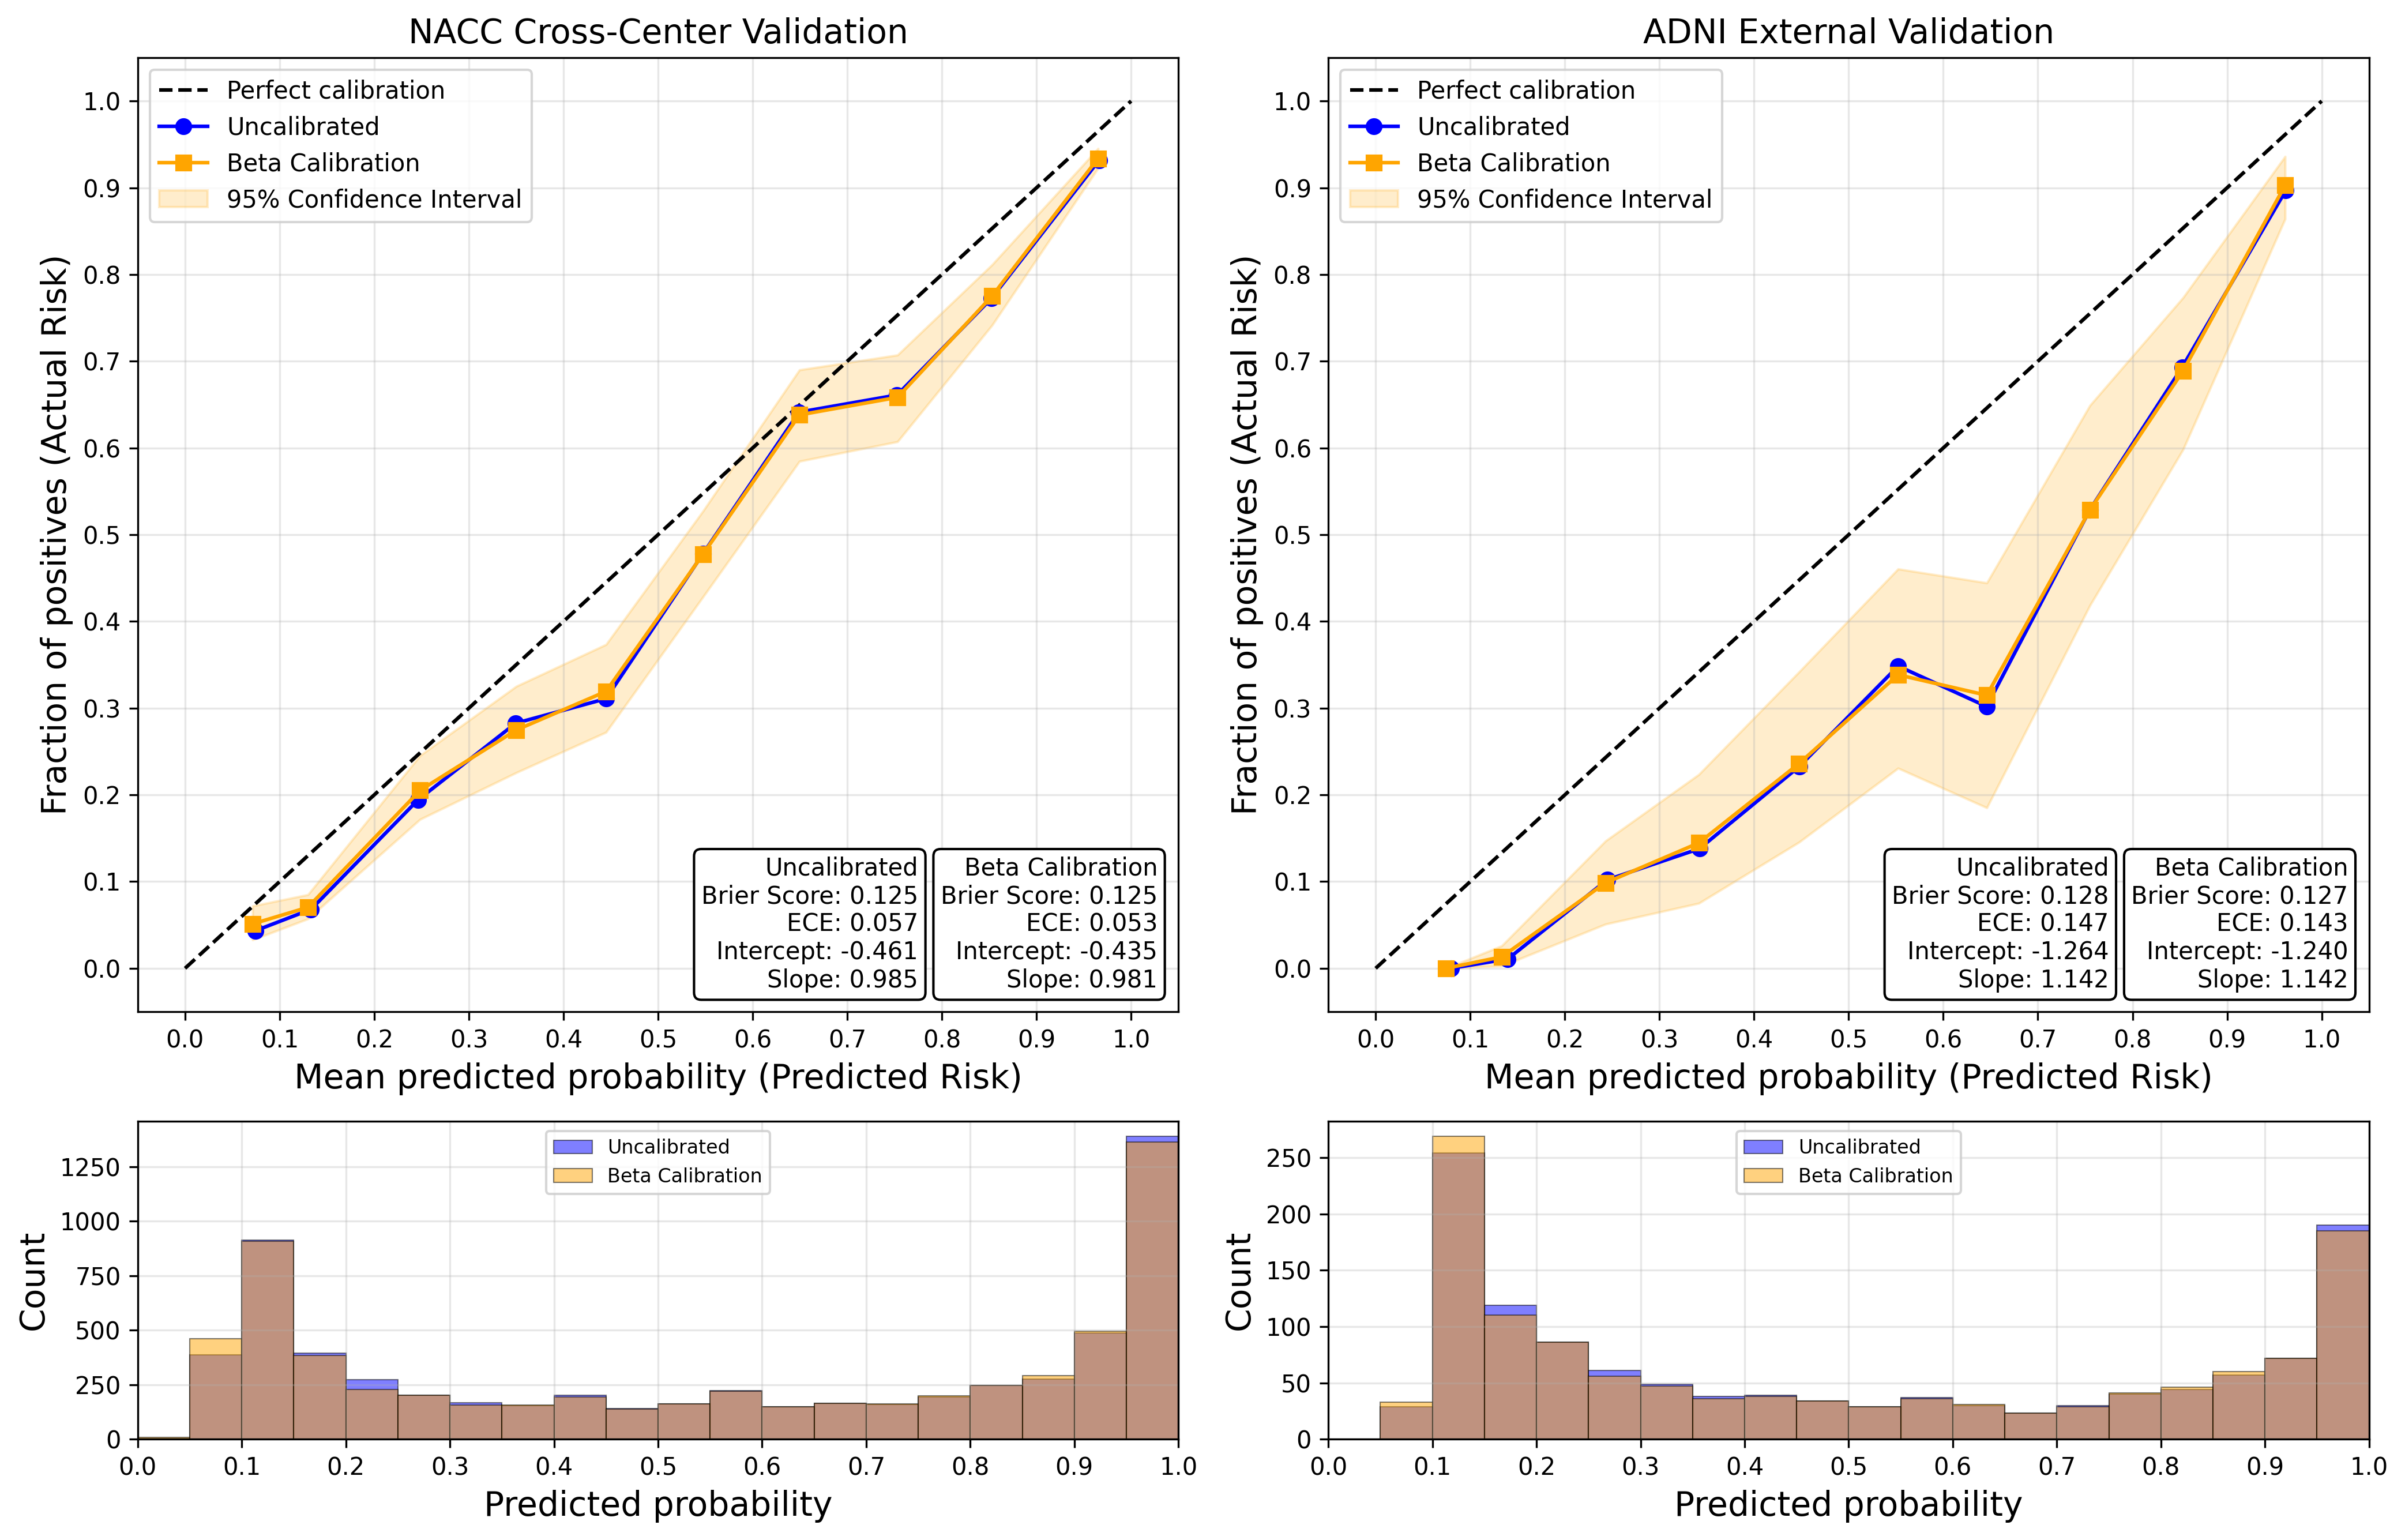
\includegraphics[width=1.0\textwidth]{figures/calibration/dementia_classification_both_calibration_curve.png}
    \caption{Model calibration curves for the CIND vs. dementia classification task}
    \begin{minipage}{\textwidth}
      \footnotesize \hl{The horizontal axis shows the predicted probability and the vertical axis shows the observed frequency of the positive class. The diagonal line represents perfect calibration, and the curves compare the model before and after beta calibration.}
    \end{minipage}
    \label{fig:cind_dementia_calib_curve}
\end{figure}

In contrast, different results were found in the ADNI external validation. A significant overestimation of the risk of dementia was observed, which is indicated by a large negative intercept of -1.264. The miscalibration was not corrected even after beta calibration. This could be explained by the fact that the calibration parameters were learned from the NACC UDS data, which could not correct the specific distribution shifts in the ADNI external dataset. As a result, the beta calibration had almost no improvement, with the ECE remaining high at 0.143.

The clinical utility of the LR model to differentiate CIND from dementia was evaluated using DCA as illustrated in Figure~\ref{fig:cind_dementia_dca}. In the NACC cross-center validation, the model had a higher net benefit than the default strategies ("treat all" and "treat none") in a wide range of probability thresholds (0.11 to 0.99). A similar excellent clinical utility was observed in the ADNI external validation, with a net benefit exceeding default strategies, specifically in probability thresholds between 0.12 and 0.89.

\begin{figure}[ht]
    \centering
    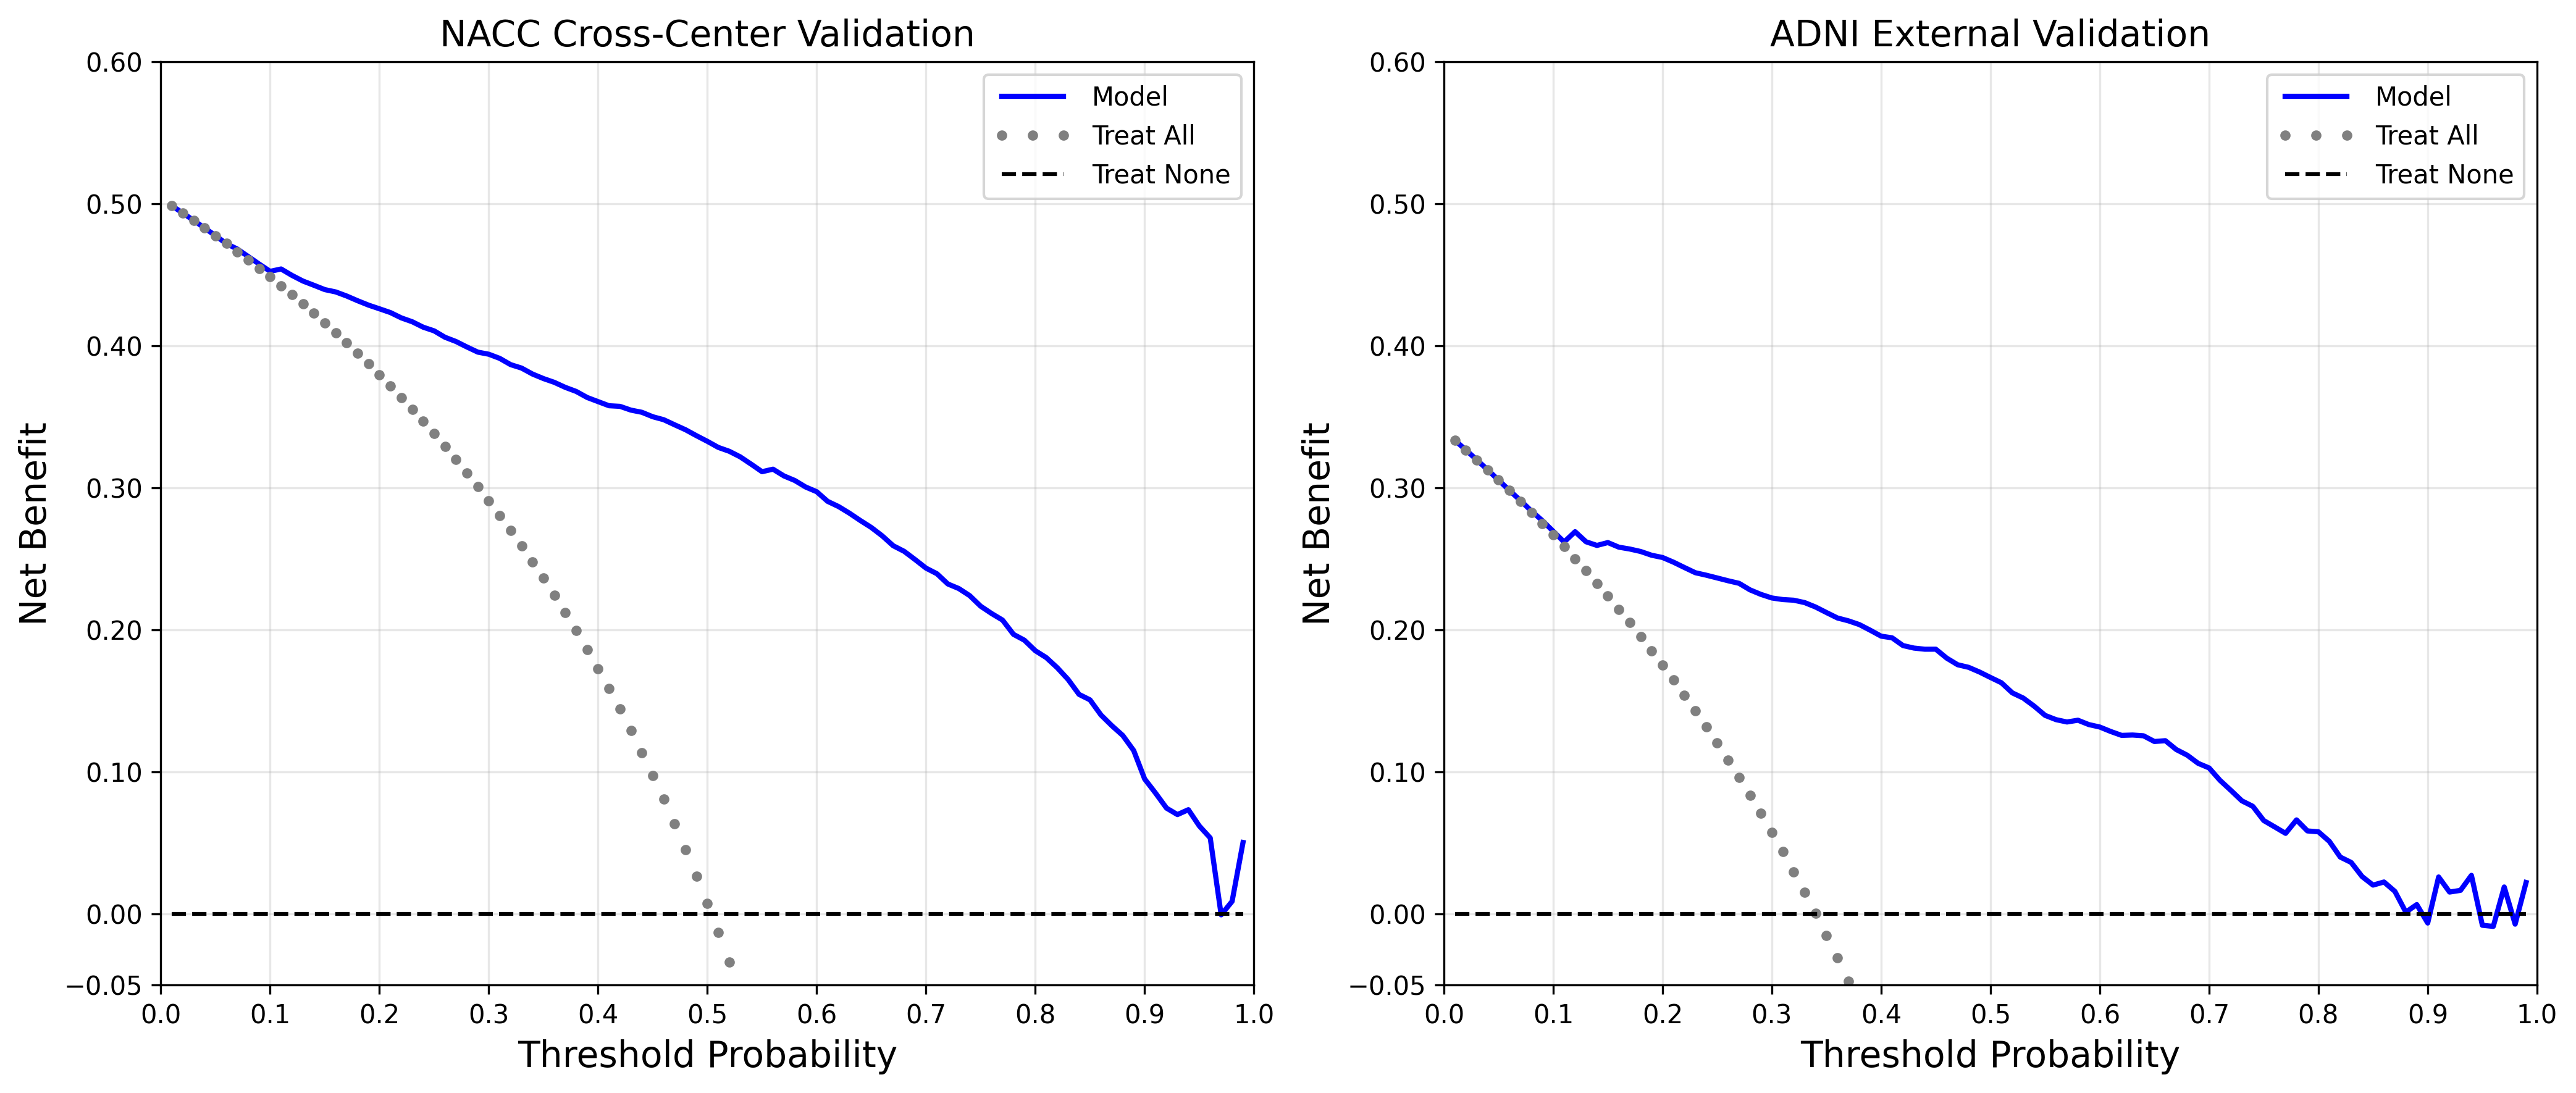
\includegraphics[width=1.0\textwidth]{figures/DCA/dementia_classification_dca_both.png}
    \caption{The decision curve analysis (DCA) for the CIND vs. dementia classification task}
    \begin{minipage}{\textwidth}
      \footnotesize This figure illustrates the DCA curves of the NACC cross-center validation (left side) and the ADNI external validation (right side). "Treat All" refers to the assumption that all subjects are predicted to have dementia, and "Treat None" refers to the assumption that none of the subjects are predicted to have CI.
    \end{minipage}
    \label{fig:cind_dementia_dca}
\end{figure}

Based on the results of the external validation process, it can be concluded that the proposed cost-effective models are reliable and generalizable. The classification models produced a high level of performance, specifically in the detection of critical cases such as dementia, when tested on independent and unseen datasets. Additionally, the models' predictions presented excellent calibration and clinical utility, especially in the NACC cross-center validation. These findings contribute to the achievement of the first research objective of this study. The results demonstrate that a cost-effective machine learning model trained on accessible data can accurately classify the current cognitive status across different clinical settings.

\subsection{Model Explainability Results}
\label{sec:cls-xai}

\subsubsection{Model Explainability Results for the NC vs. CI Classification Task}
The global feature importance ranking of this task is provided in Figure~\ref{figure:nc_ci_feature_importance} for both external validation datasets. The features are sorted on the basis of their mean absolute SHapley values obtained from the SHapley Additive exPlanations (\acrshort{SHAP}). The feature importance ranking in both external validation datasets is highly consistent, with Spearman’s coefficient of 0.93 ($p$ < 0.05). This strong positive correlation indicates that the model relies on a stable set of clinical patterns to predict cognitive impairment, regardless of the population or data source. In both tests, functional activities were identified as the most critical predictors. Specifically, REMDATES, TRAVEL, BILLS and TAXES were consistently ranked as the top four most important features. This indicates the influence of executive function on the model's classification of cases as NC or CI. On the other hand, demographic factors such as NACCAGE (age) and SEX showed less importance compared to the other features. MEMPROB ranked higher in the NACC cross-center validation compared to the ADNI external validation. This might reflect the diagnostic procedures used in these different studies. In addition, the feature importance rank slightly differed in the least important features. NACCAGE ranked as the least important feature after ANX and SEX in the ADNI external validation compared to the NACC cross-center validation.

\begin{figure}[ht]
    \centering
    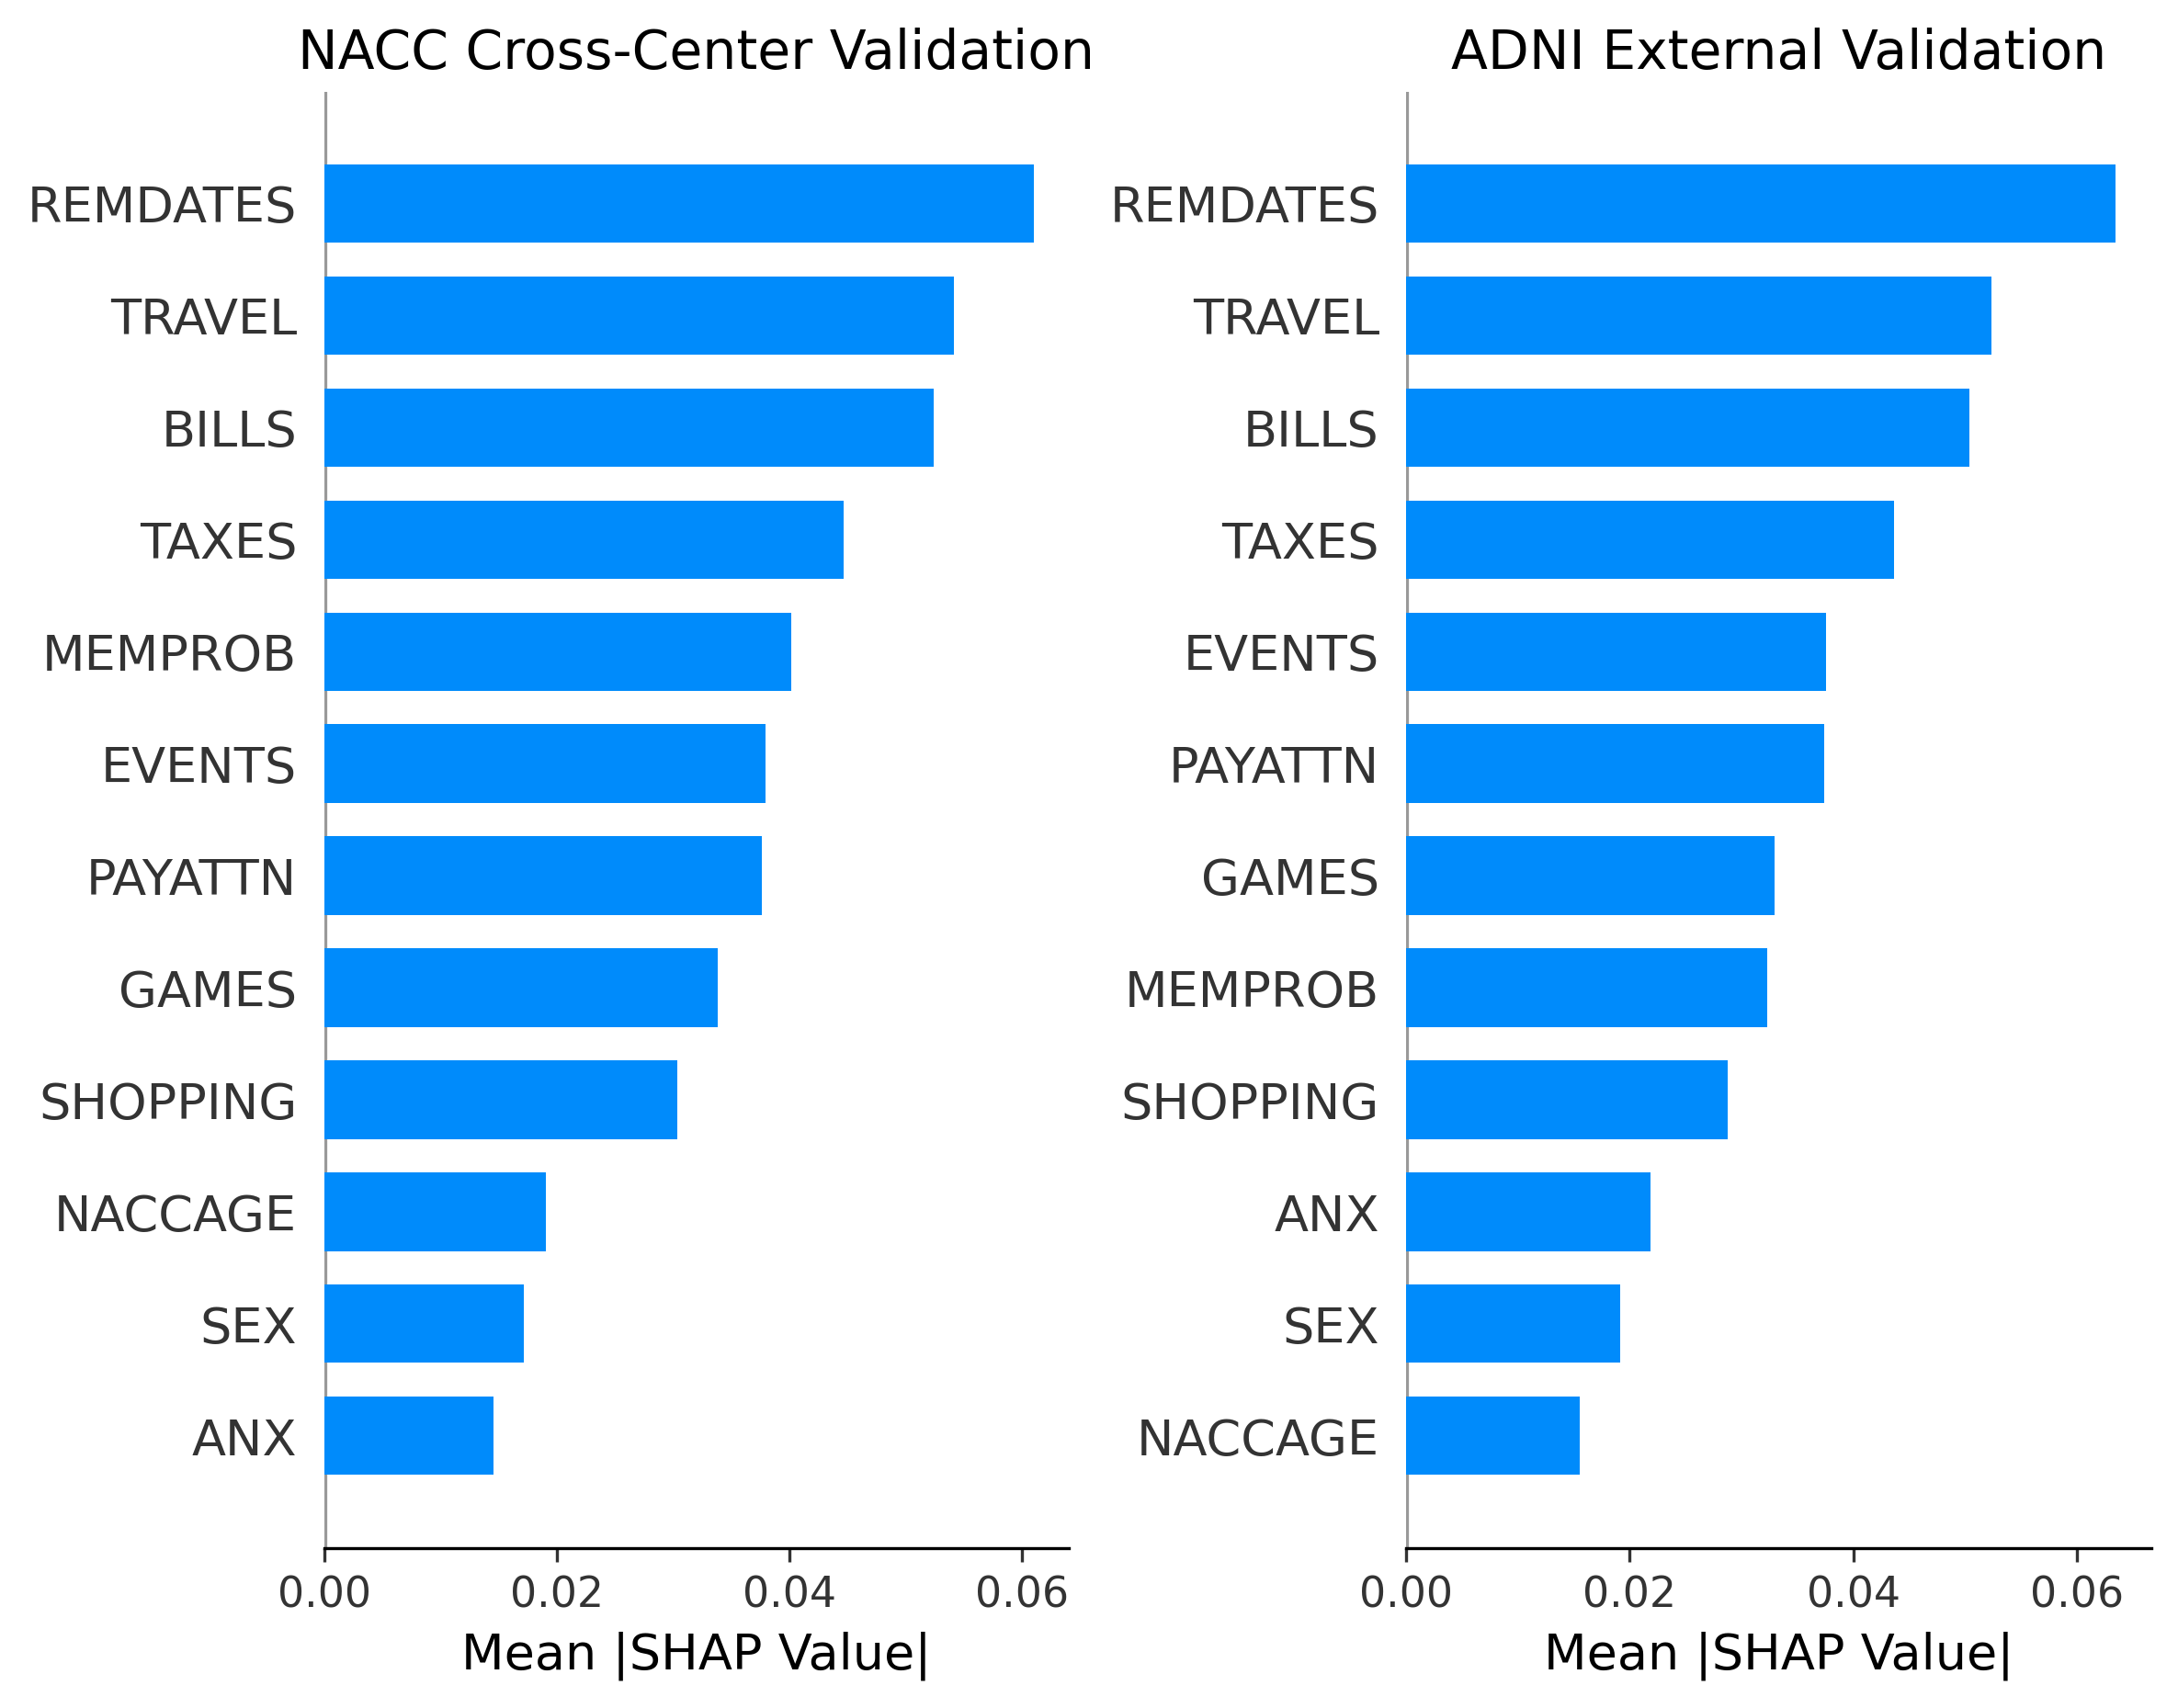
\includegraphics[width=1.0\textwidth]{figures/XAI/impaired_classification_both_feature_importance_comparison.png}
    \caption{Feature importance in the NACC cross-center validation and the ADNI external validation for the NC vs. CI classification task}
    \begin{minipage}{\textwidth}
      \footnotesize \hl{The bars represent the mean absolute SHAP value of each feature, which ranks the contribution of the feature to the model prediction in the two validation datasets.}
    \end{minipage}
    \label{figure:nc_ci_feature_importance}
\end{figure}

Regarding the local explanation, the waterfall plots in Figure~\ref{figure:nc_ci_pos_waterfall} explain the prediction of two correctly classified CI instances from the ADNI external validation. Both instances have similar predicted probabilities of approximately 55\%. \textit{Instance A} predicted with CI due to reported memory problems (MEMPROB) and anxiety (ANX) despite the ability to normally perform all functional activities based on the items in the FAQ. On the other hand, \textit{Instance B} represents an older subject who suffers from difficulty in handling financial matters, specifically paying bills (BILLS) and doing taxes (TAXES). This comparison highlights the model's capability to detect CI through different pathways: one driven by memory and psychological symptoms (\textit{Instance A}) and another driven by specific functional decline in complex tasks (Instance B).

\begin{figure}[ht]
    \centering
    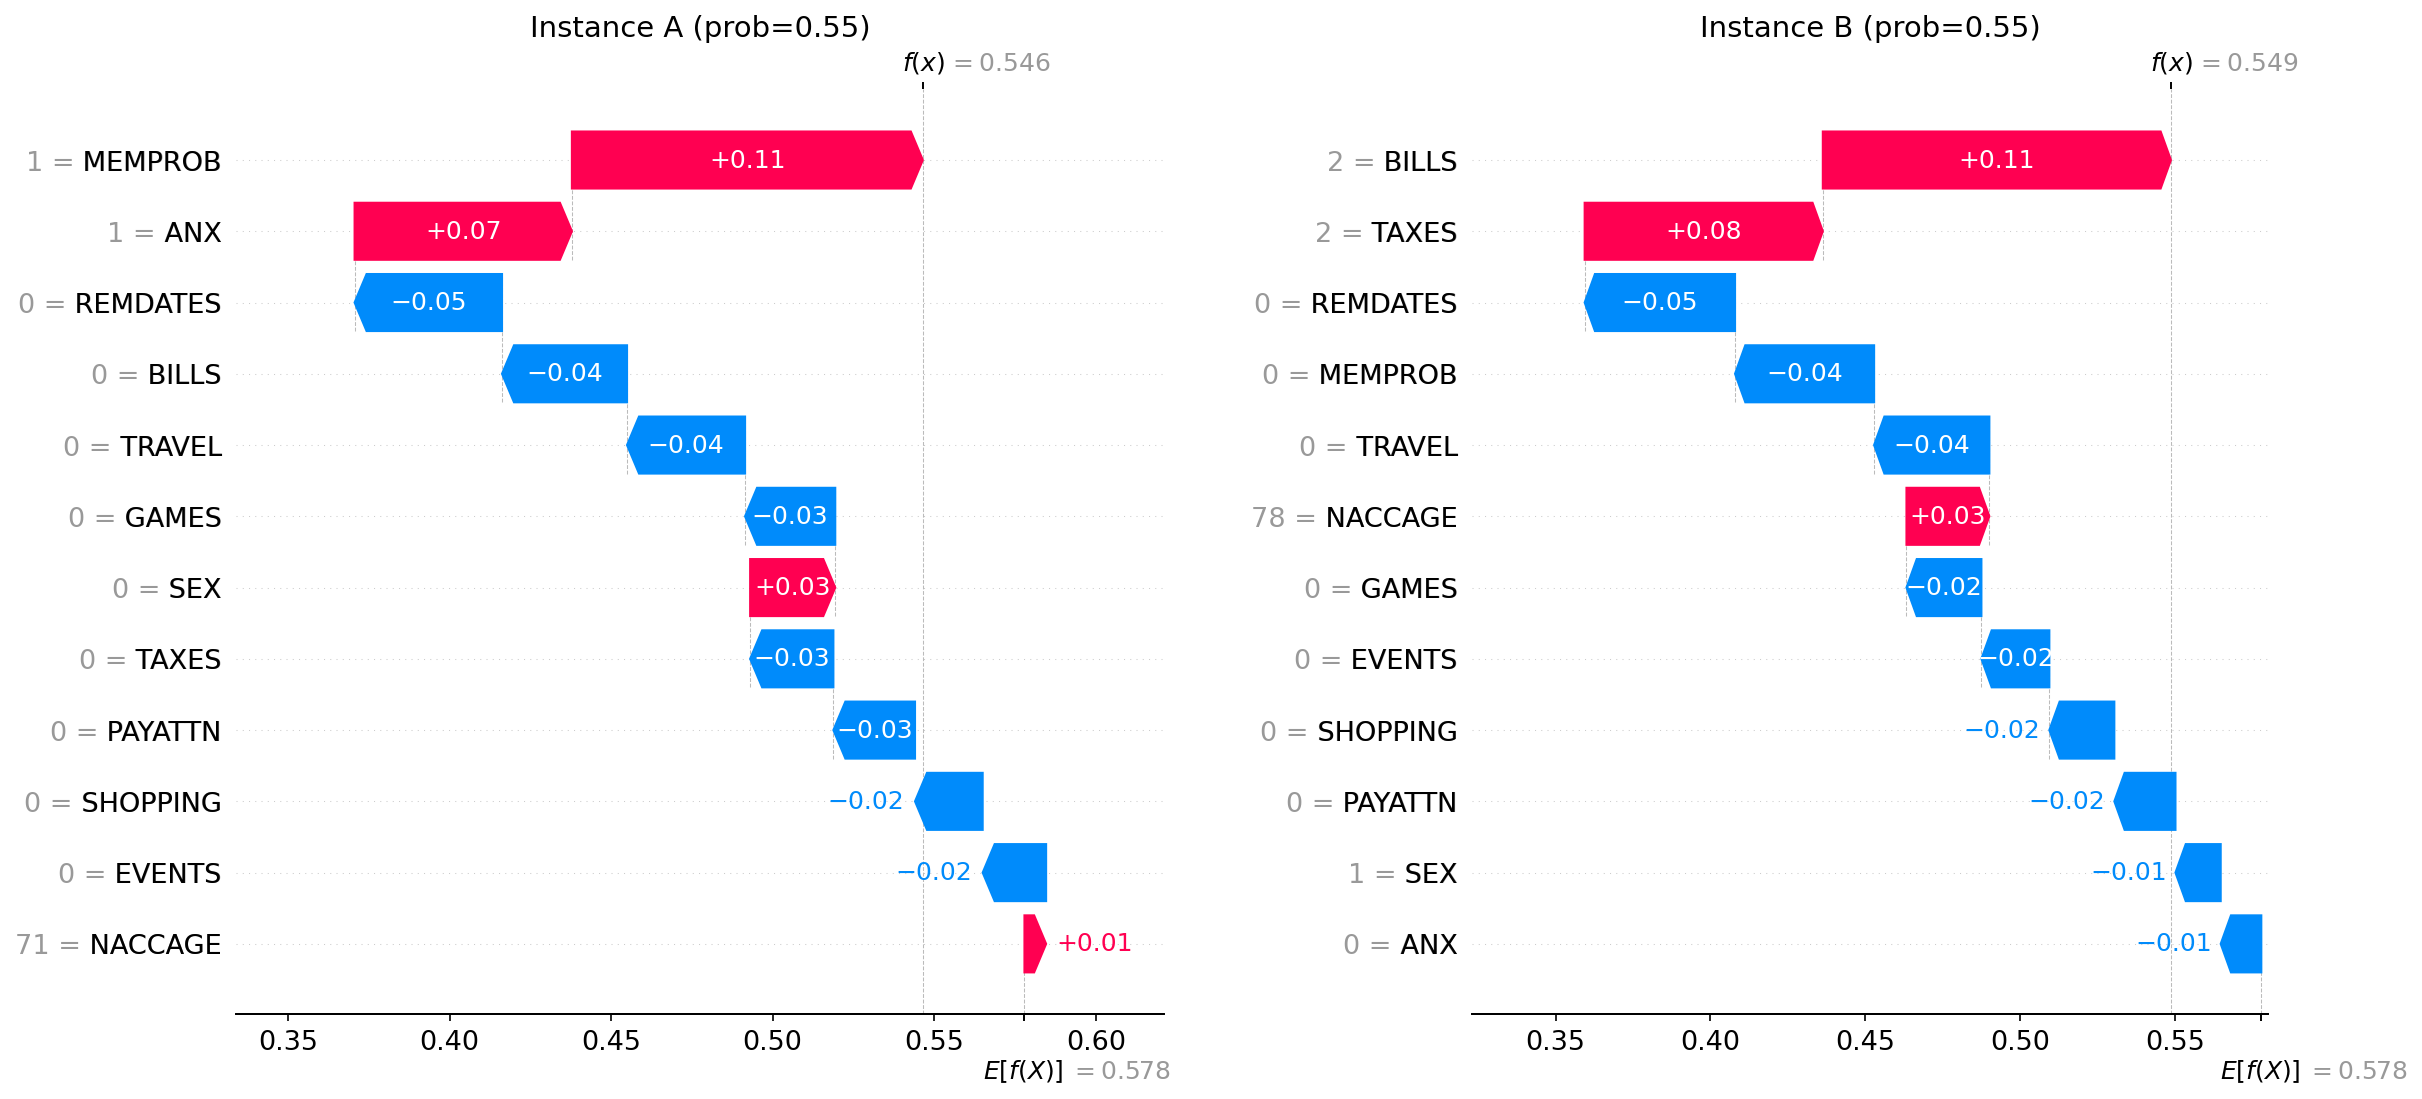
\includegraphics[width=1.0\textwidth]{figures/XAI/impaired_classification_adni_true_positive_waterfall.png}
    \caption{SHAP waterfall plots for two instances correctly classified as cognitive impairment}
    \begin{minipage}{\textwidth}
      \footnotesize \hl{The plot shows how the value of each feature shifts the prediction from the base value to the final predicted probability for a single instance.}
    \end{minipage}
    \label{figure:nc_ci_pos_waterfall}
\end{figure}

Looking at the correctly classified NC instances in Figure~\ref{figure:nc_ci_neg_waterfall}, \textit{Instance A} has a predicted probability of around 44\%. The main reason for classifying this instance as NC is the ability to normally perform most functional activities, pushing the predicted probability 27\% away from CI. This overturned the highest increased risk due to the difficulty in remembering dates and appointments (REMDATES) and the age of 86. On the other hand, \textit{Instance B} represents a male subject who has anxiety and has never paid bills (BILLS). These factors increased his risk of CI compared to \textit{Instance A}. However, \textit{Instance B} was also predicted as NC with a similar probability of around 43\% due to a normal functional profile (including normal REMDATES), normal memory, and younger age than \textit{Instance A}.

\begin{figure}[ht]
    \centering
    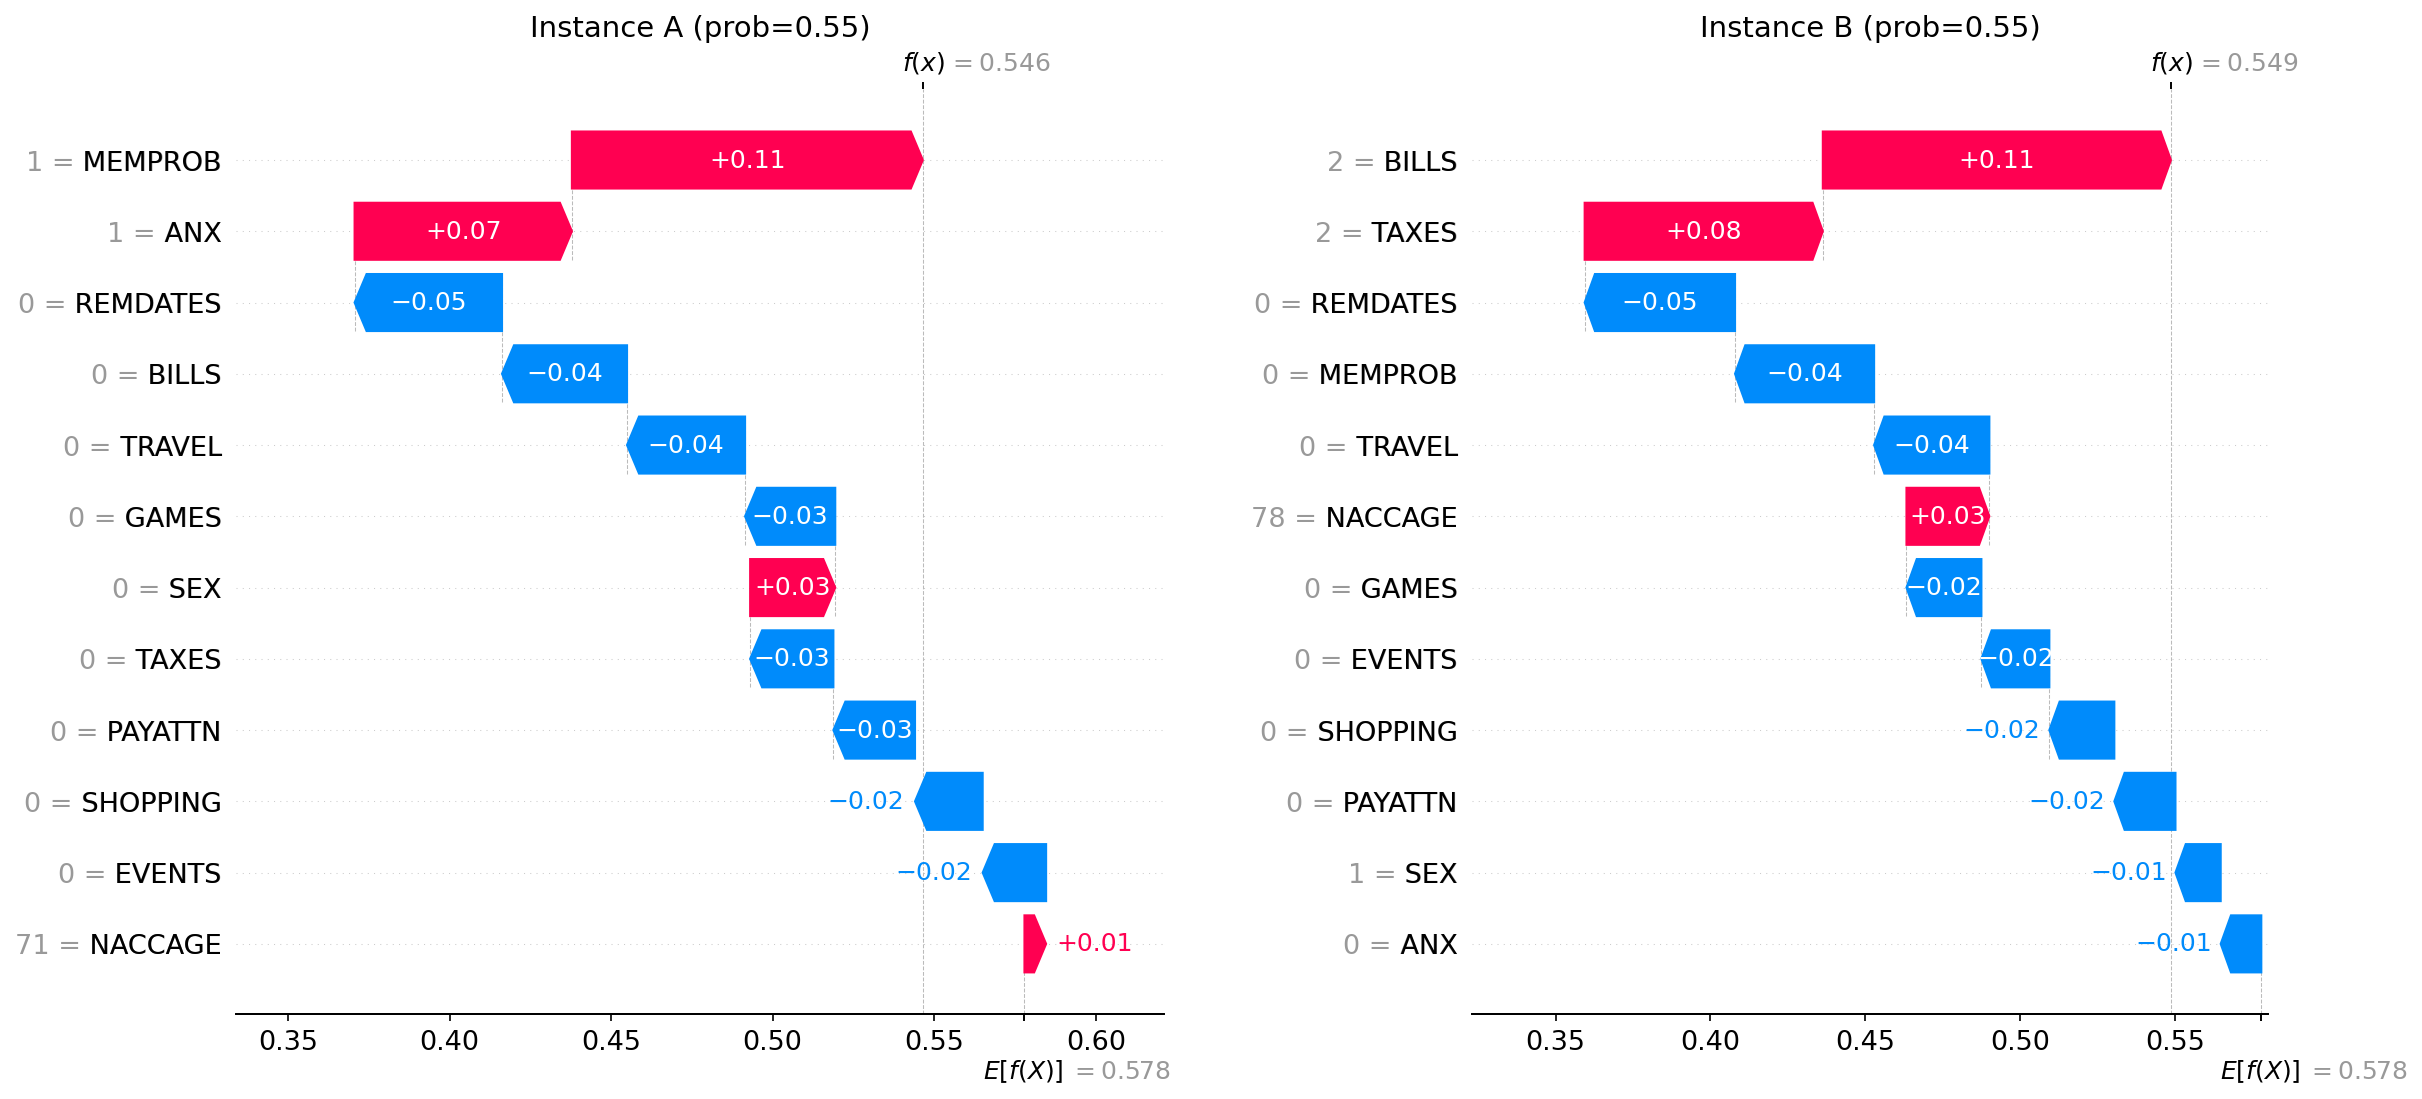
\includegraphics[width=1.0\textwidth]{figures/XAI/impaired_classification_adni_true_positive_waterfall.png}
    \caption{SHAP waterfall plots for two instances correctly classified as normal cognition}
    \begin{minipage}{\textwidth}
      \footnotesize \hl{The plot shows how the value of each feature shifts the prediction from the base value to the final predicted probability for a single instance.}
    \end{minipage}
    \label{figure:nc_ci_neg_waterfall}
\end{figure}

The analysis of the counterfactual explanation performed by Diverse Counterfactual Explanations (\acrshort{DiCE}) is shown in Figure~\ref{figure:nc_ci_dice_stat}. DiCE was able to generate at least one counterfactual example for approximately 99\% of the ADNI samples (mean = 2.66, median = 2). Most instances had more than one suggestion for risk intervention (counterfactual examples), while only about 11\% of instances had up to five counterfactual examples.

\begin{figure}[ht]
    \centering
    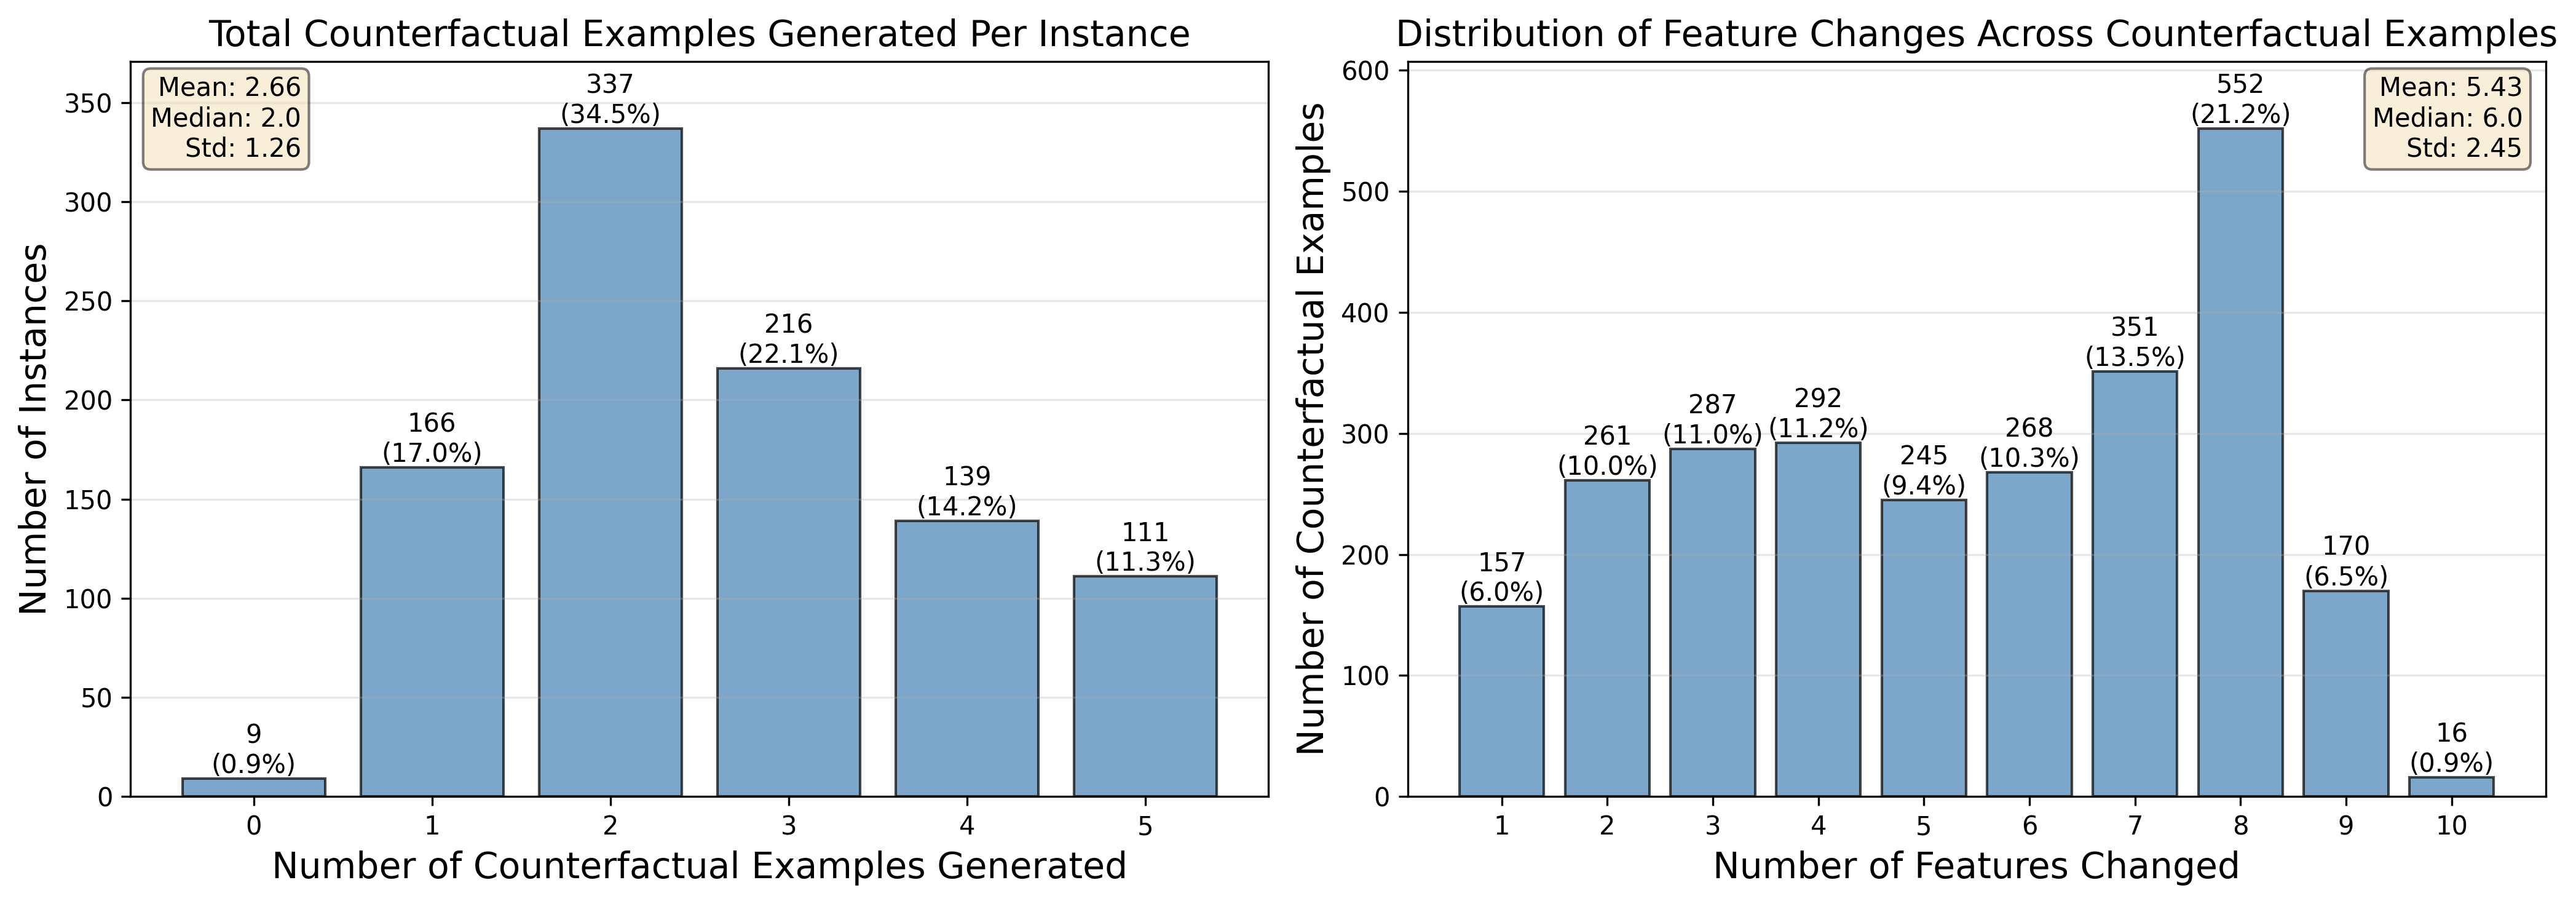
\includegraphics[width=1.0\textwidth]{figures/XAI/impaired_classification_adni_kdtree_dice_stats.png}
    \caption{Summary of generated counterfactual examples for changing the model classification from cognitive impairment to normal cognition}
    \label{figure:nc_ci_dice_stat}
\end{figure}

As shown in the right chart of Figure~\ref{figure:nc_ci_dice_stat}, of the 10 modifiable features, on average about 5 to 6 features needed to be changed to generate valid counterfactuals. The majority of counterfactual examples required modifying between 2 and 9 features, with the highest frequency being 8 features (21.2\%). A very small percentage of counterfactual examples required altering all 10 features. Similar results were observed in the counterfactual explanation of the NACC cross-center validation dataset which can be found in Figure~\ref{figure:dice-nacc-task1-apdx} in the appendix.

The most effective features for risk interventions can be analyzed using the feature importance bar chart in Figure~\ref{figure:nc_ci_dice_feature_importance}. Functional activities related to FAQ were the most frequently modified features. The top three features are handling taxes (76\%), remembering dates (74\%), and paying bills (71\%). In contrast, reported memory problems (MEMPROB) and anxiety (ANX) were less frequently changed, with scores of 17\% and 32\%, respectively. Table~\ref{table:cfe-adni-task1-apdx} in the appendix illustrates counterfactual examples generated for a random subject classified as CI to reverse the estimated outcome to NC.

\begin{figure}[ht]
    \centering
    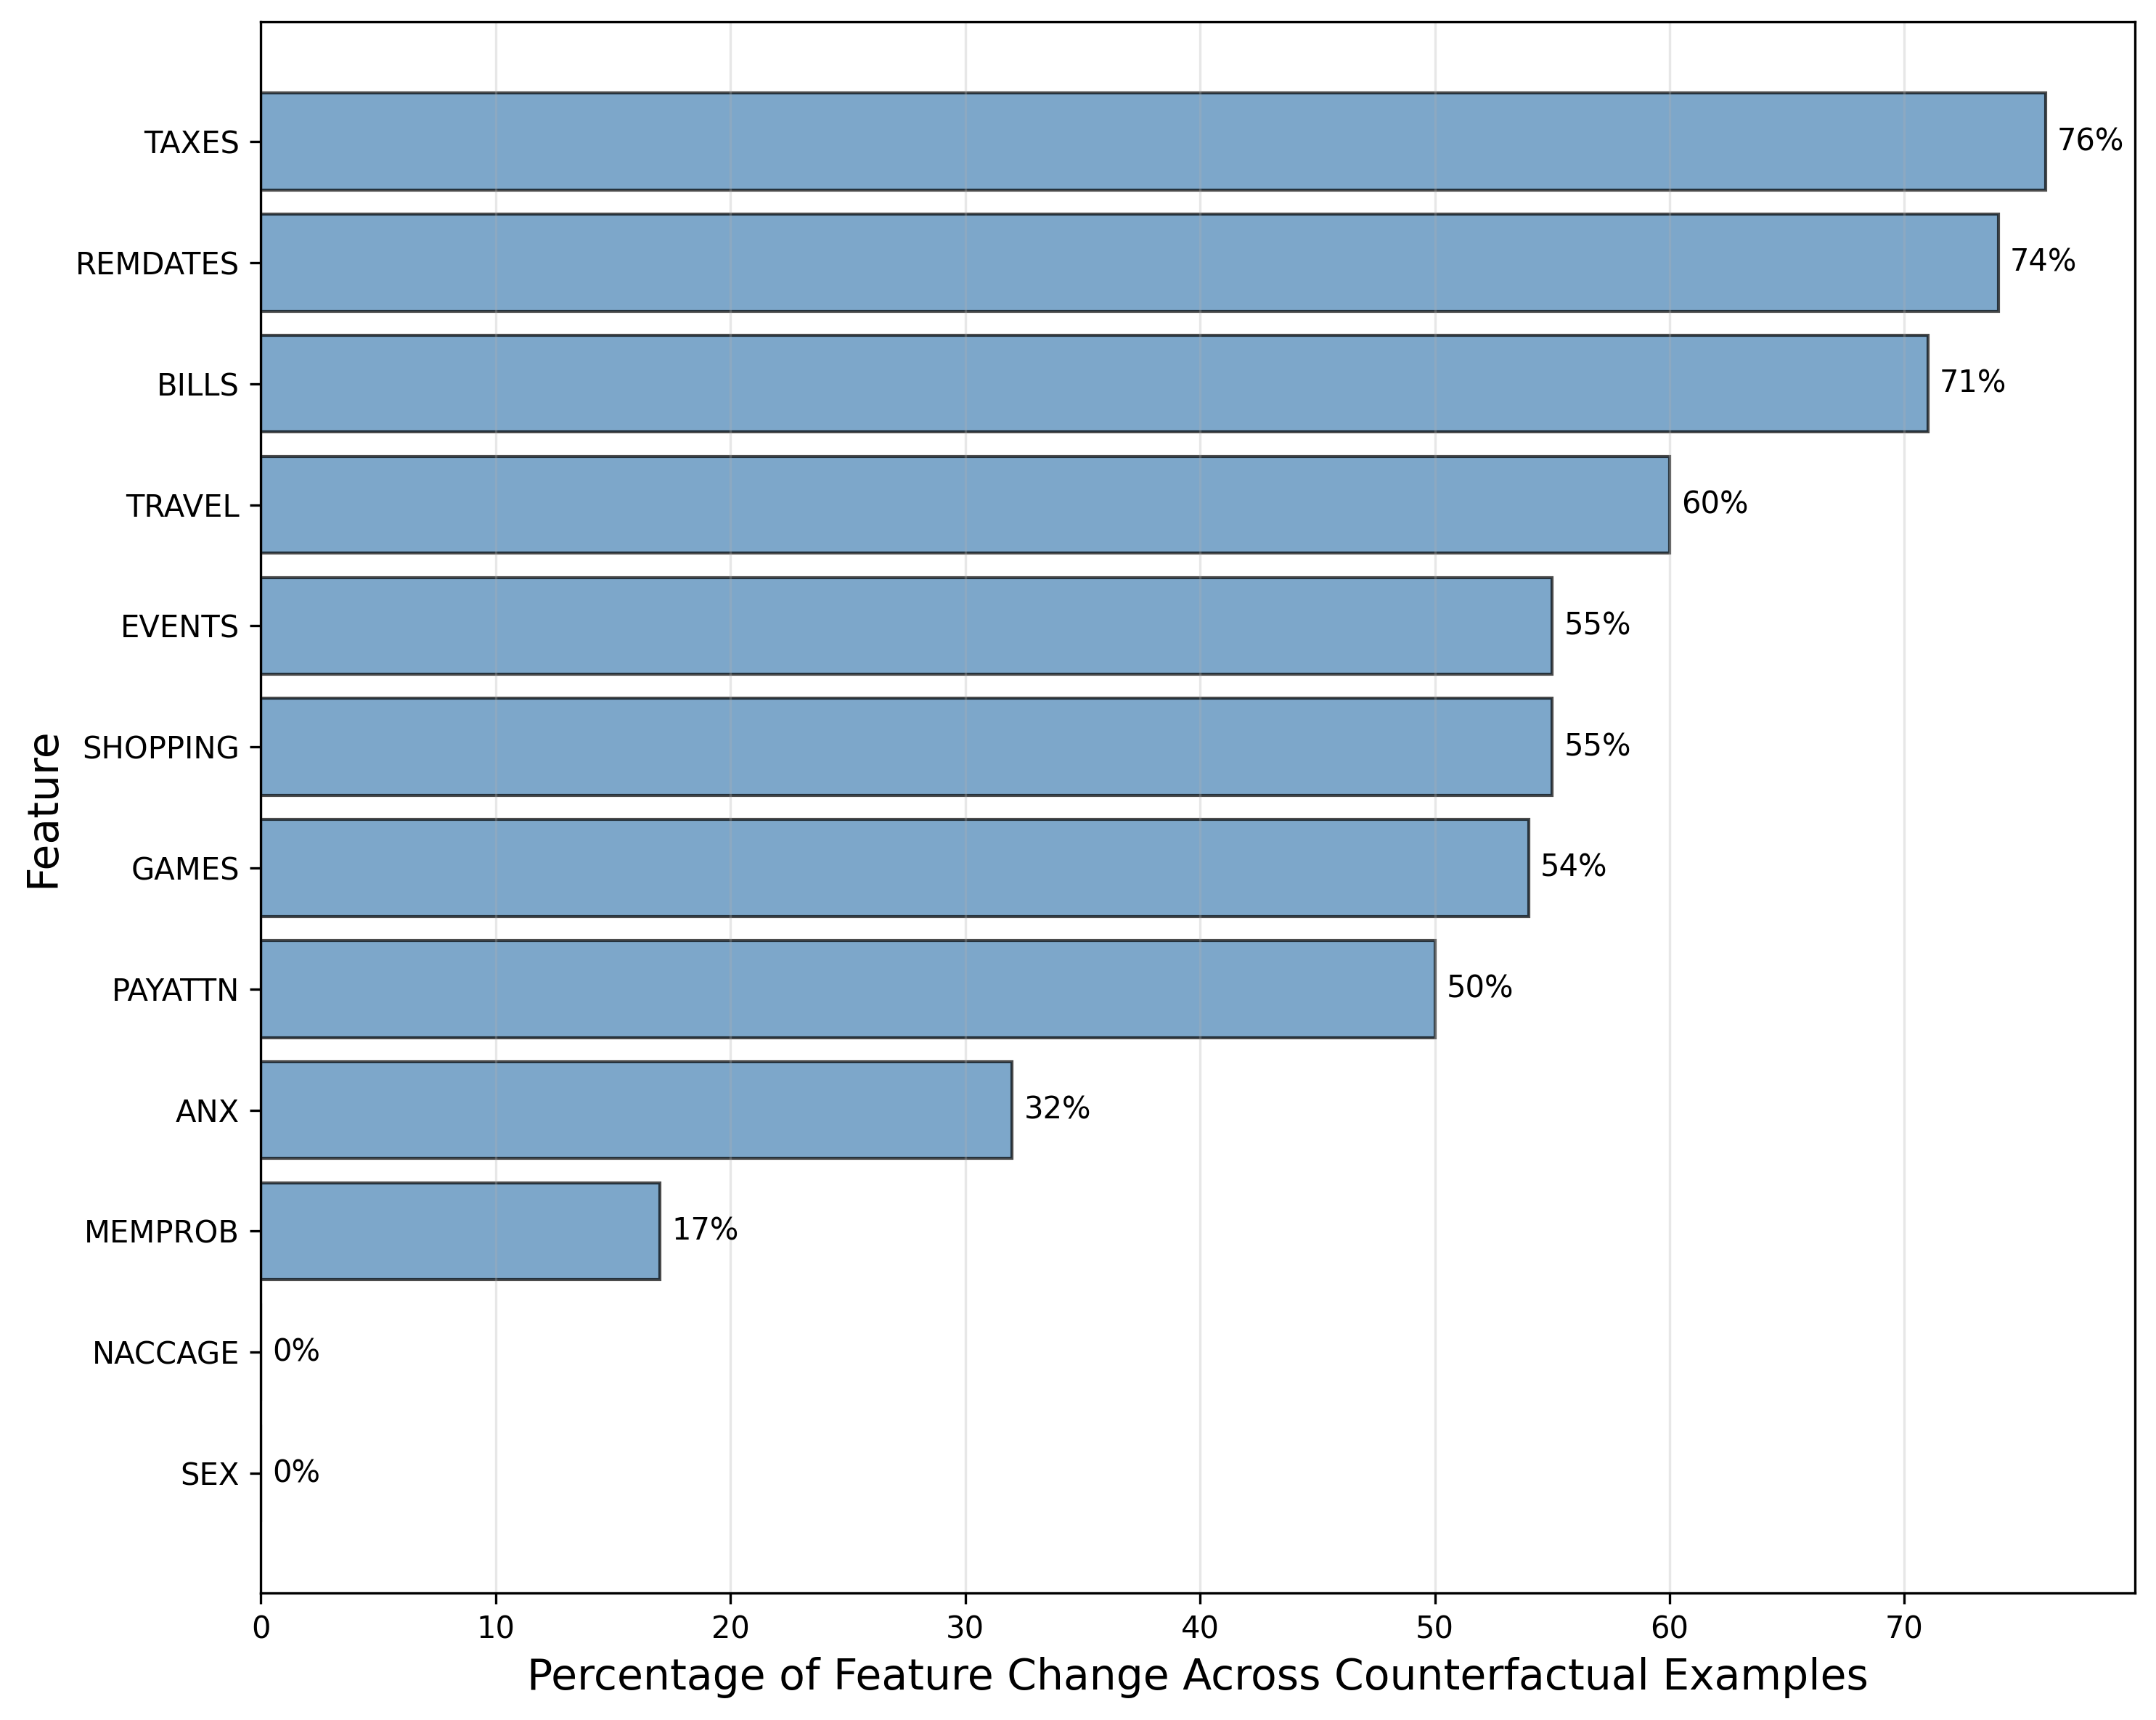
\includegraphics[width=1.0\textwidth]{figures/XAI/impaired_classification_adni_kdtree_dice_global_importance.png}
    \caption{Feature importance ranking based on counterfactual explanations for the NC vs. CI classification task}
    \begin{minipage}{\textwidth}
      \footnotesize The features are ranked based on the percentage of times they were modified to generate valid counterfactual examples. The rank highlights the most critical features for risk intervention. Demographic features (NACCAGE and SEX) show 0\% importance because they were set as invariable features in the counterfactual generation process.
    \end{minipage}
    \label{figure:nc_ci_dice_feature_importance}
\end{figure}

\subsubsection{Model Explainability Results for the CIND vs. Dementia Classification Task}
The global feature importance ranking for the CIND vs. dementia classification task is presented in Figure~\ref{figure:cind_dementia_feature_importance}. The figure shows the mean absolute SHAP values of the features in both the NACC cross-center validation and the ADNI external validation. The Spearman’s rank correlation coefficient of 0.98 ($p$ < 0.05) demonstrates a high degree of consistency in the ranking of feature importance between these two external validation datasets. Similarly to the NC vs. CI classification tasks, functional activity features emerged as the dominant factors influencing the model's predictions in both external validation datasets. The three most important predictors are BILLS, TRAVEL, and EVENTS. In contrast, features such as primary language (PRIMLANG) and changes of appetite (APP) consistently showed a lower importance. 

\begin{figure}[ht]
    \centering
    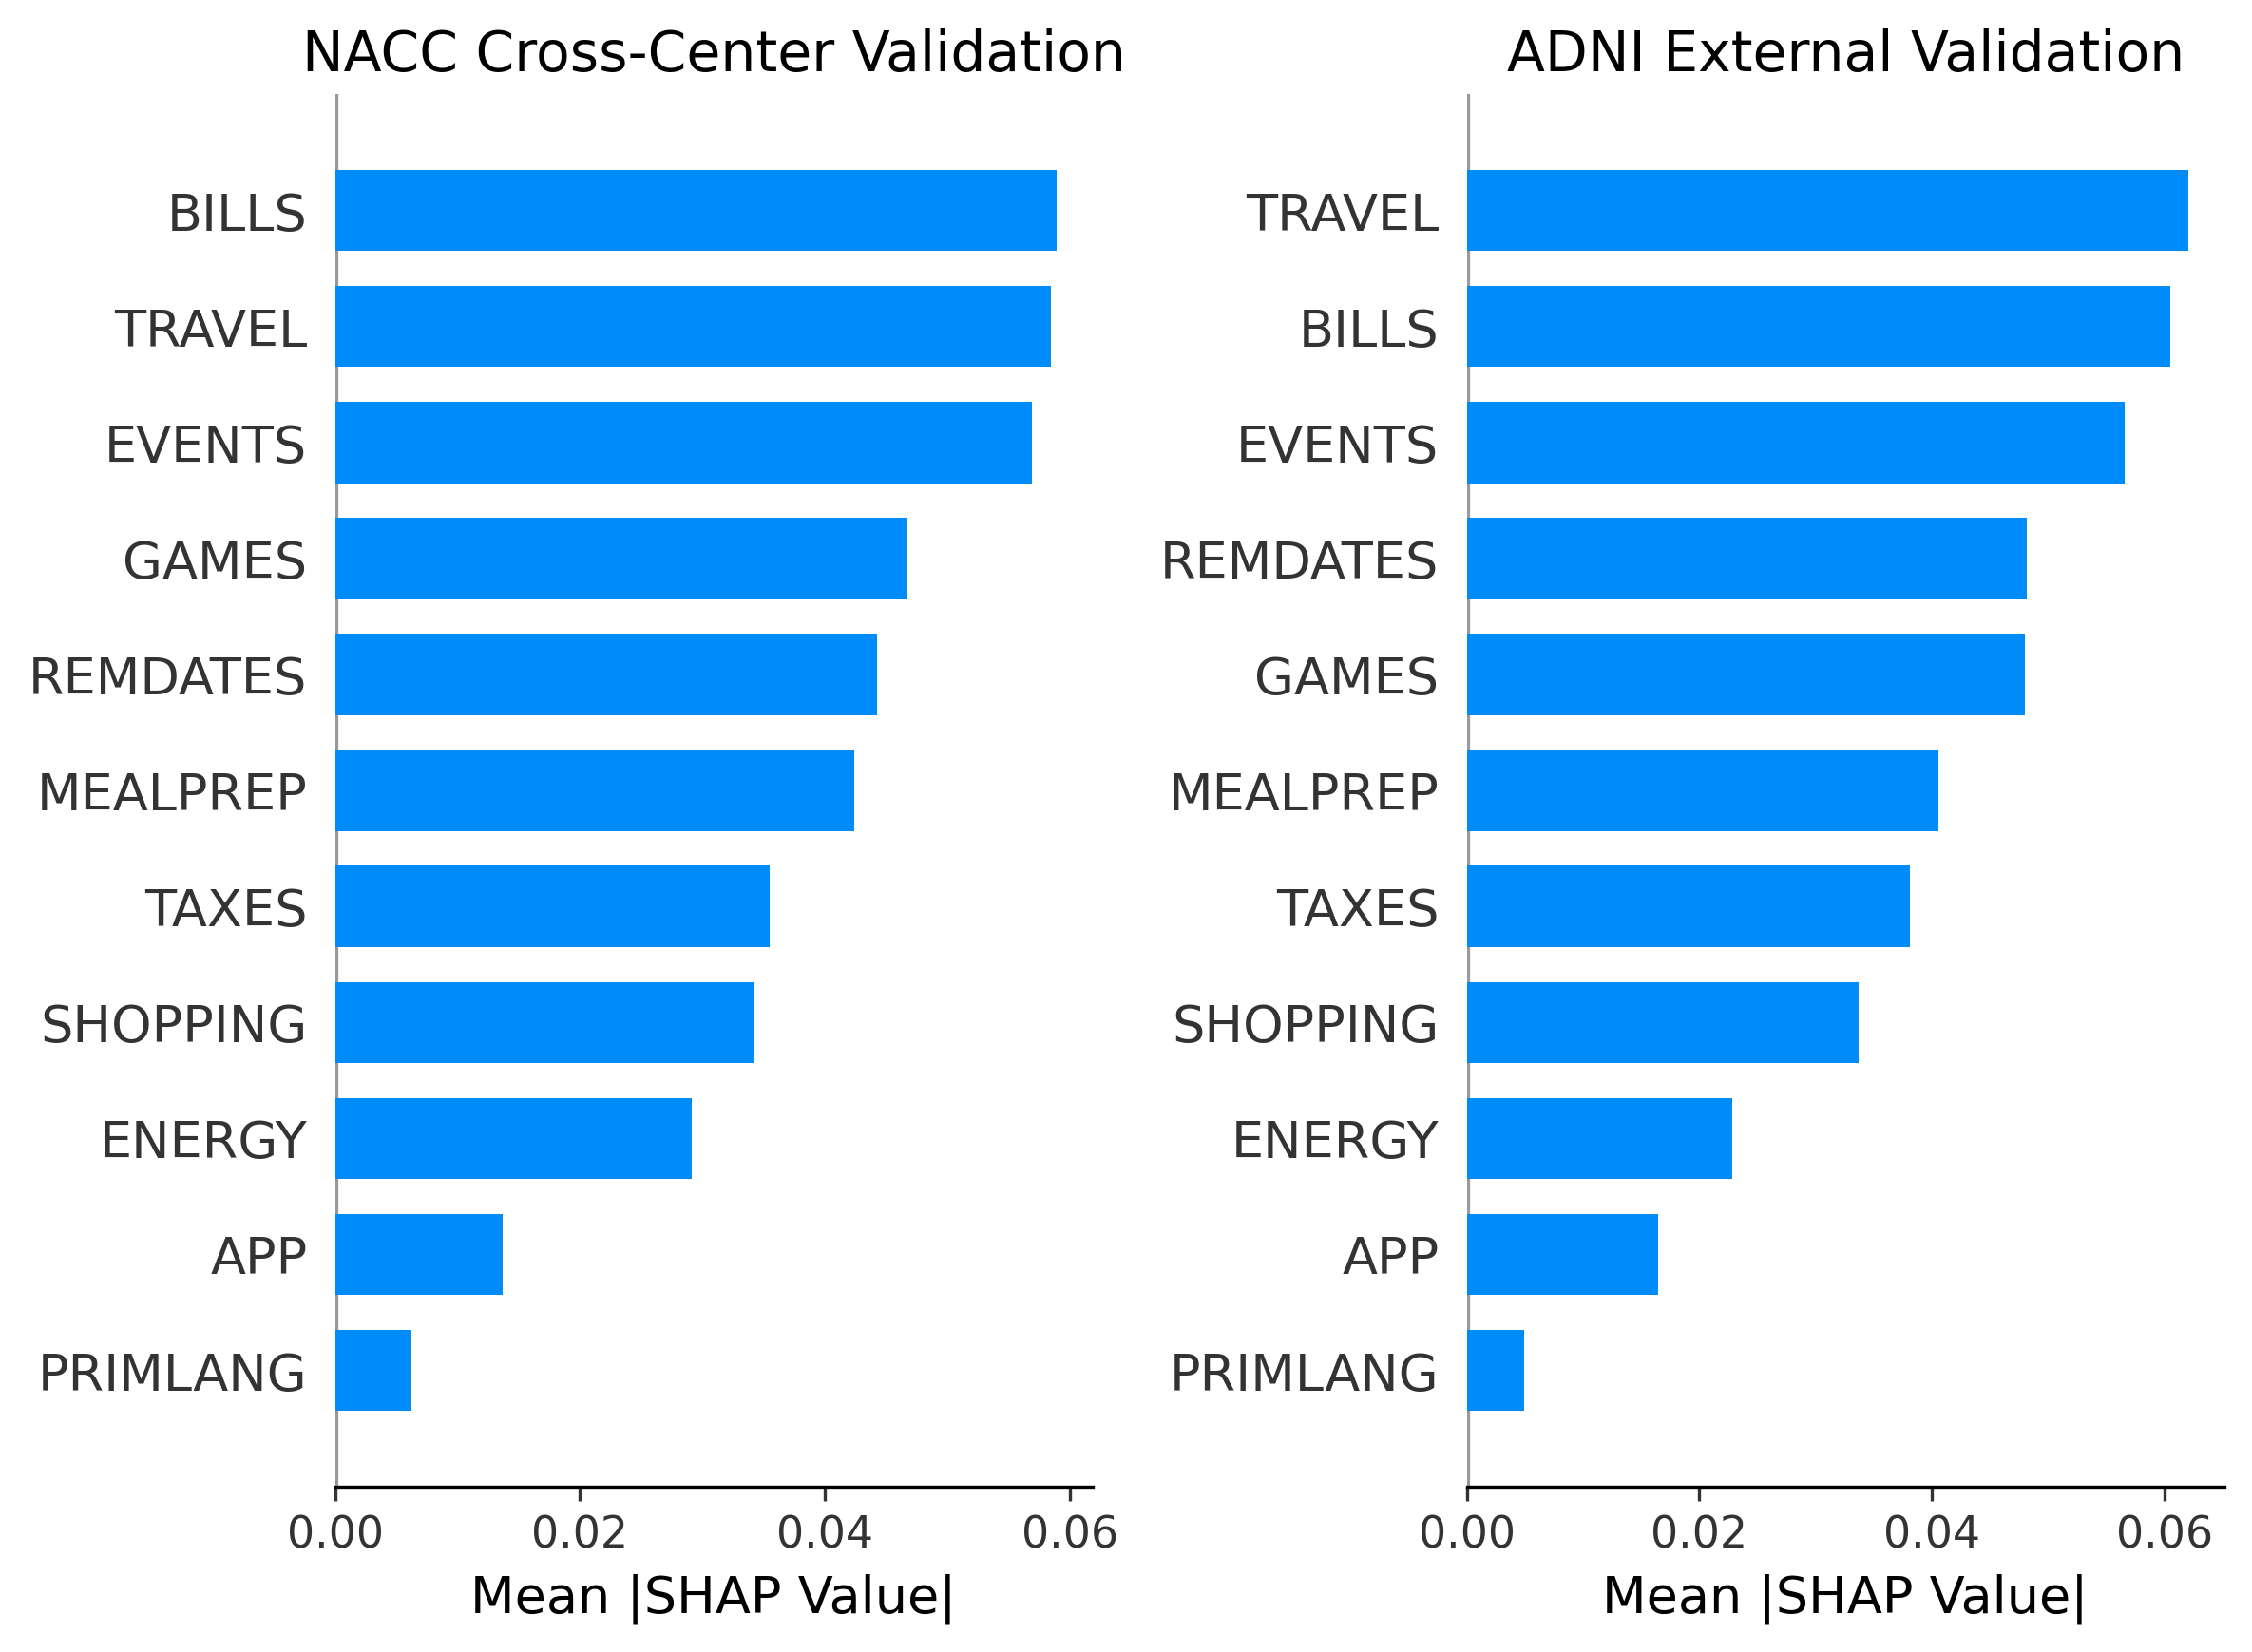
\includegraphics[width=1.0\textwidth]{figures/XAI/dementia_classification_both_feature_importance_comparison.png}
    \caption{Feature importance in the NACC cross-center validation and the ADNI external validation for the CIND vs. dementia classification task}
    \begin{minipage}{\textwidth}
      \footnotesize \hl{The bars represent the mean absolute SHAP value of each feature, which ranks the contribution of the feature to the model prediction in the two validation datasets.}
    \end{minipage}
    \label{figure:cind_dementia_feature_importance}
\end{figure}

To evaluate the local explanation of the model, two correctly classified instances from each class with distinct feature profiles have been analyzed to demonstrate the model's ability to capture heterogeneous patterns. For instances classified as dementia, both \textit{Instance A} and \textit{Instance B} in Figure~\ref{figure:cind_dementia_pos_waterfall} had similar predicted probabilities of approximately 58\% and 57\%, respectively. However, both instances have different contributing factors. \textit{Instance A} requires assistance with filling taxes (TAXES) and has difficulty tracking current events (EVENTS), in addition to reported appetite changes (APP). In contrast, \textit{Instance B} presented a different functional decline profile, as it requires assistance with traveling (TRAVEL) and remembering dates (REMDATES).

\begin{figure}[ht]
    \centering
    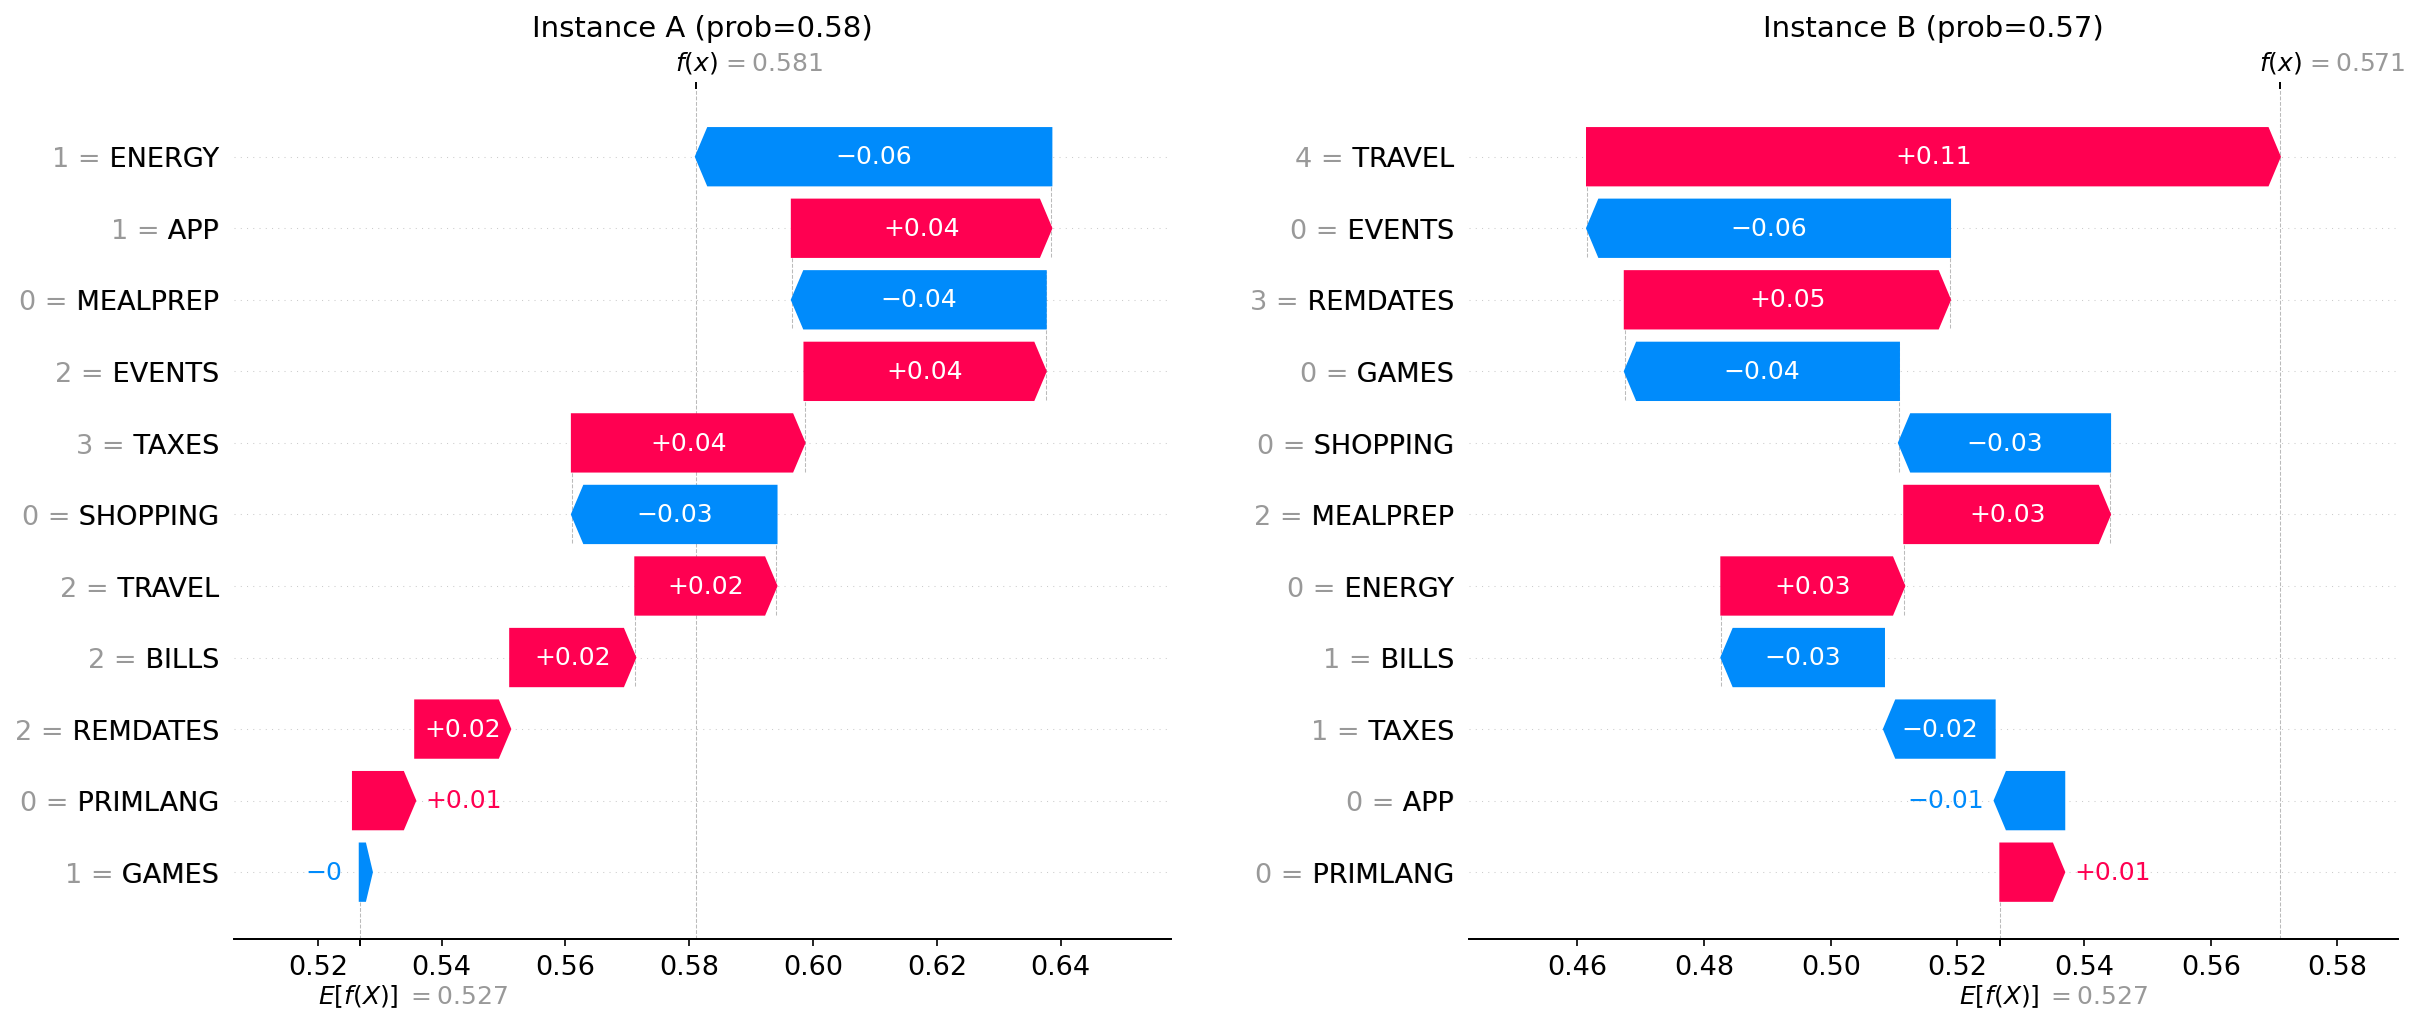
\includegraphics[width=1.0\textwidth]{figures/XAI/dementia_classification_adni_true_positive_waterfall.png}
    \caption{SHAP waterfall plots for two instances correctly classified as dementia}
    \begin{minipage}{\textwidth}
      \footnotesize \hl{The plot shows how the value of each feature shifts the prediction from the base value to the final predicted probability for a single instance.}
    \end{minipage}
    \label{figure:cind_dementia_pos_waterfall}
\end{figure}

The other two randomly selected CIND instances in Figure~\ref{figure:cind_dementia_neg_waterfall} were classified with probabilities of 40\%. \textit{Instance A} represented a profile of functional independence, with the ability to normally handle bills, taxes, events, and meal preparation. This level of independence was strong enough to minimize the risk of dementia introduced by appetite changes and other risk factors. With a different pattern, the classification of \textit{Instance B} as CIND was driven by the ability to normally track events and remember dates regardless of the difficulty in handling financial tasks.

\begin{figure}[ht]
    \centering
    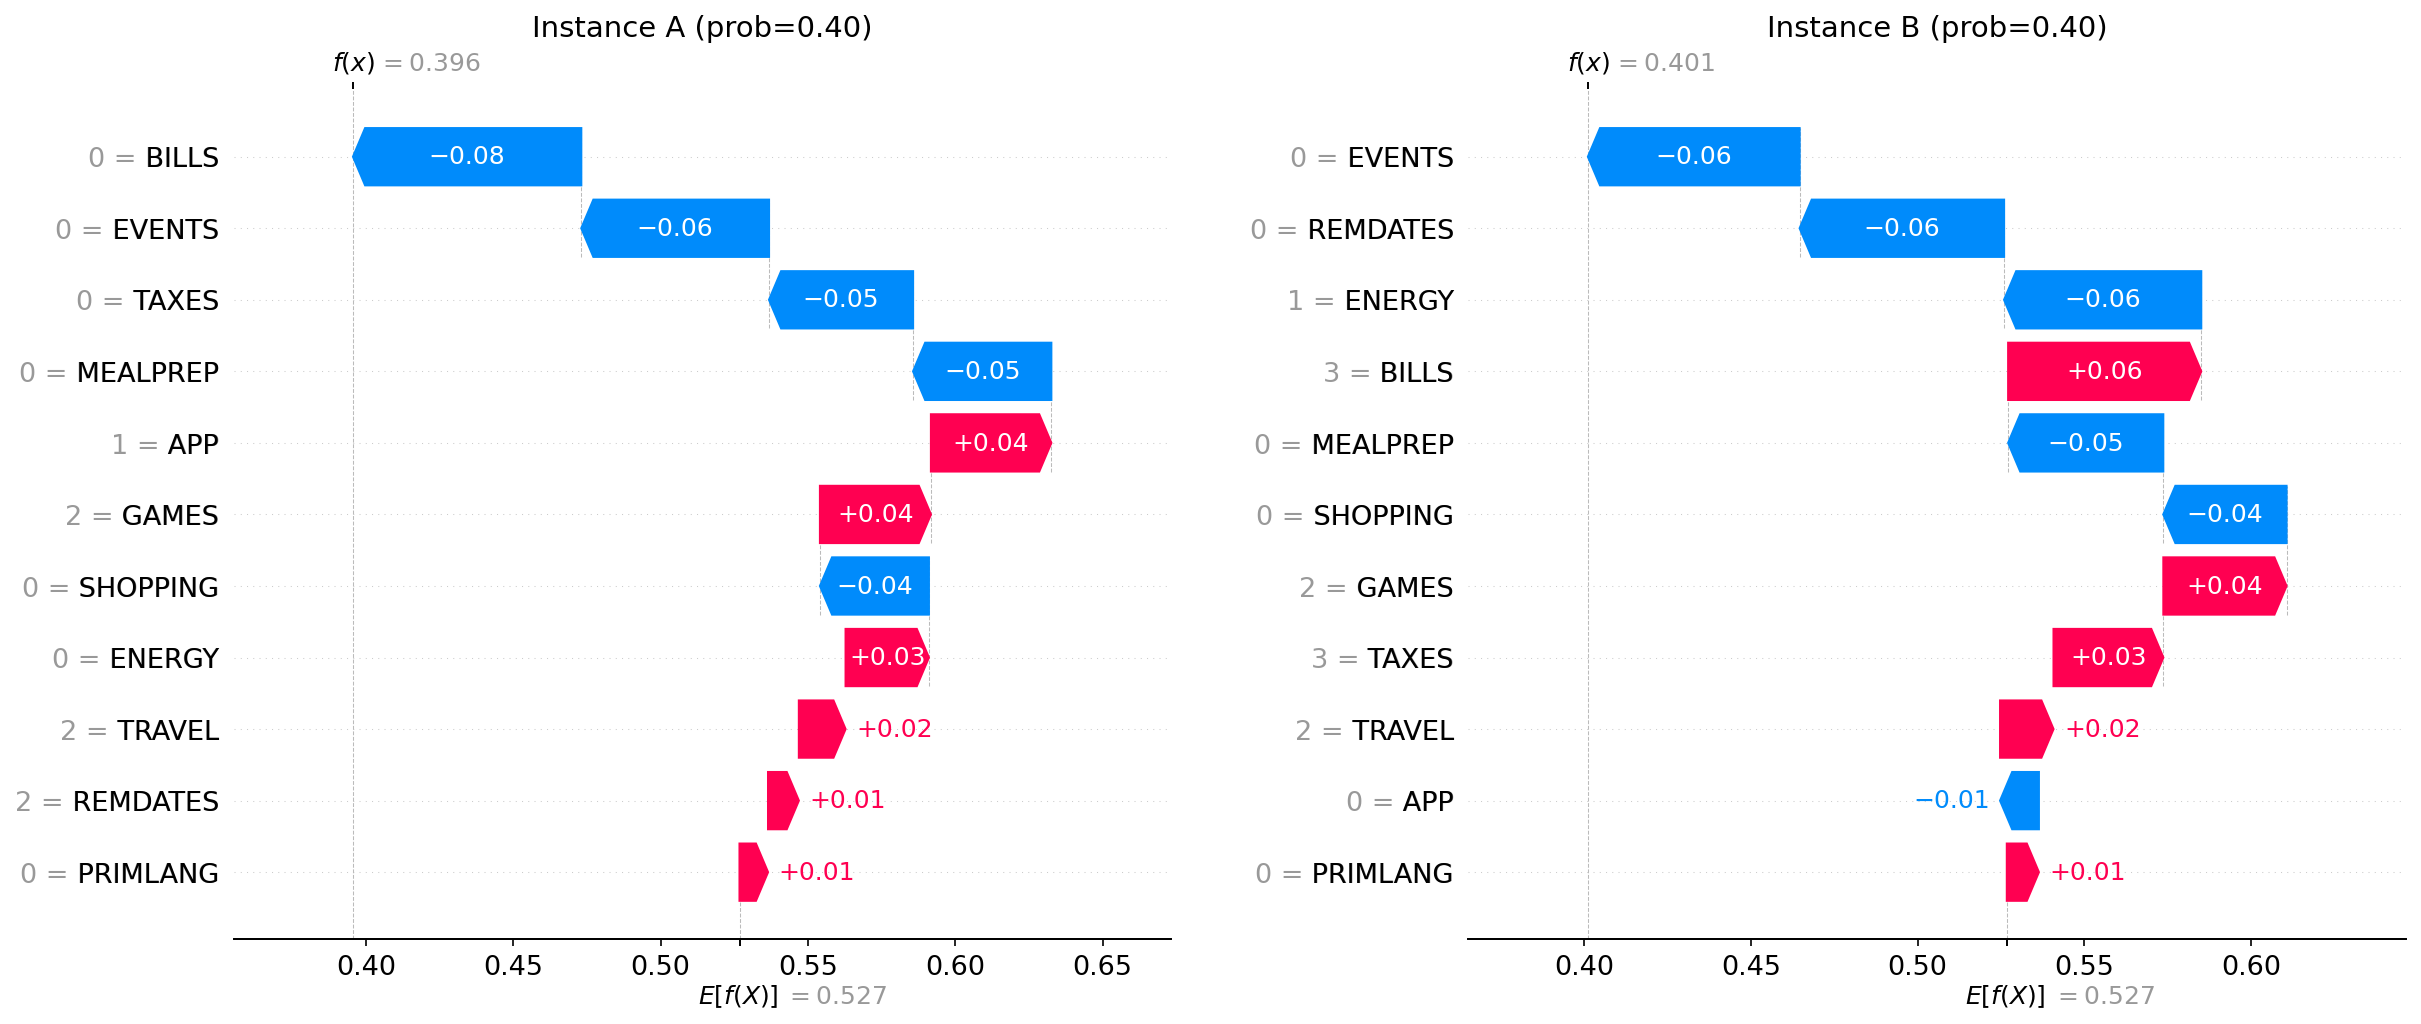
\includegraphics[width=1.0\textwidth]{figures/XAI/dementia_classification_adni_true_negative_waterfall.png}
    \caption{SHAP waterfall plots for two instances correctly classified as cognitive impairment but not dementia (CIND)}
    \begin{minipage}{\textwidth}
      \footnotesize \hl{The plot shows how the value of each feature shifts the prediction from the base value to the final predicted probability for a single instance.}
    \end{minipage}
    \label{figure:cind_dementia_neg_waterfall}
\end{figure}

In regard to the results of the counterfactual explanation in the ADNI external validation, counterfactual examples were generated for more than 91\% of the instances (mean = 4.38, median = 5). The majority of instances (83.6\%) had five counterfactual examples generated, while only 8.6\% of the instances had no counterfactual examples found. The analysis of the counterfactual explanation performed by the DiCE method is shown in Figure~\ref{figure:cind_dementia_dice_stat}.

\begin{figure}[ht]
    \centering
    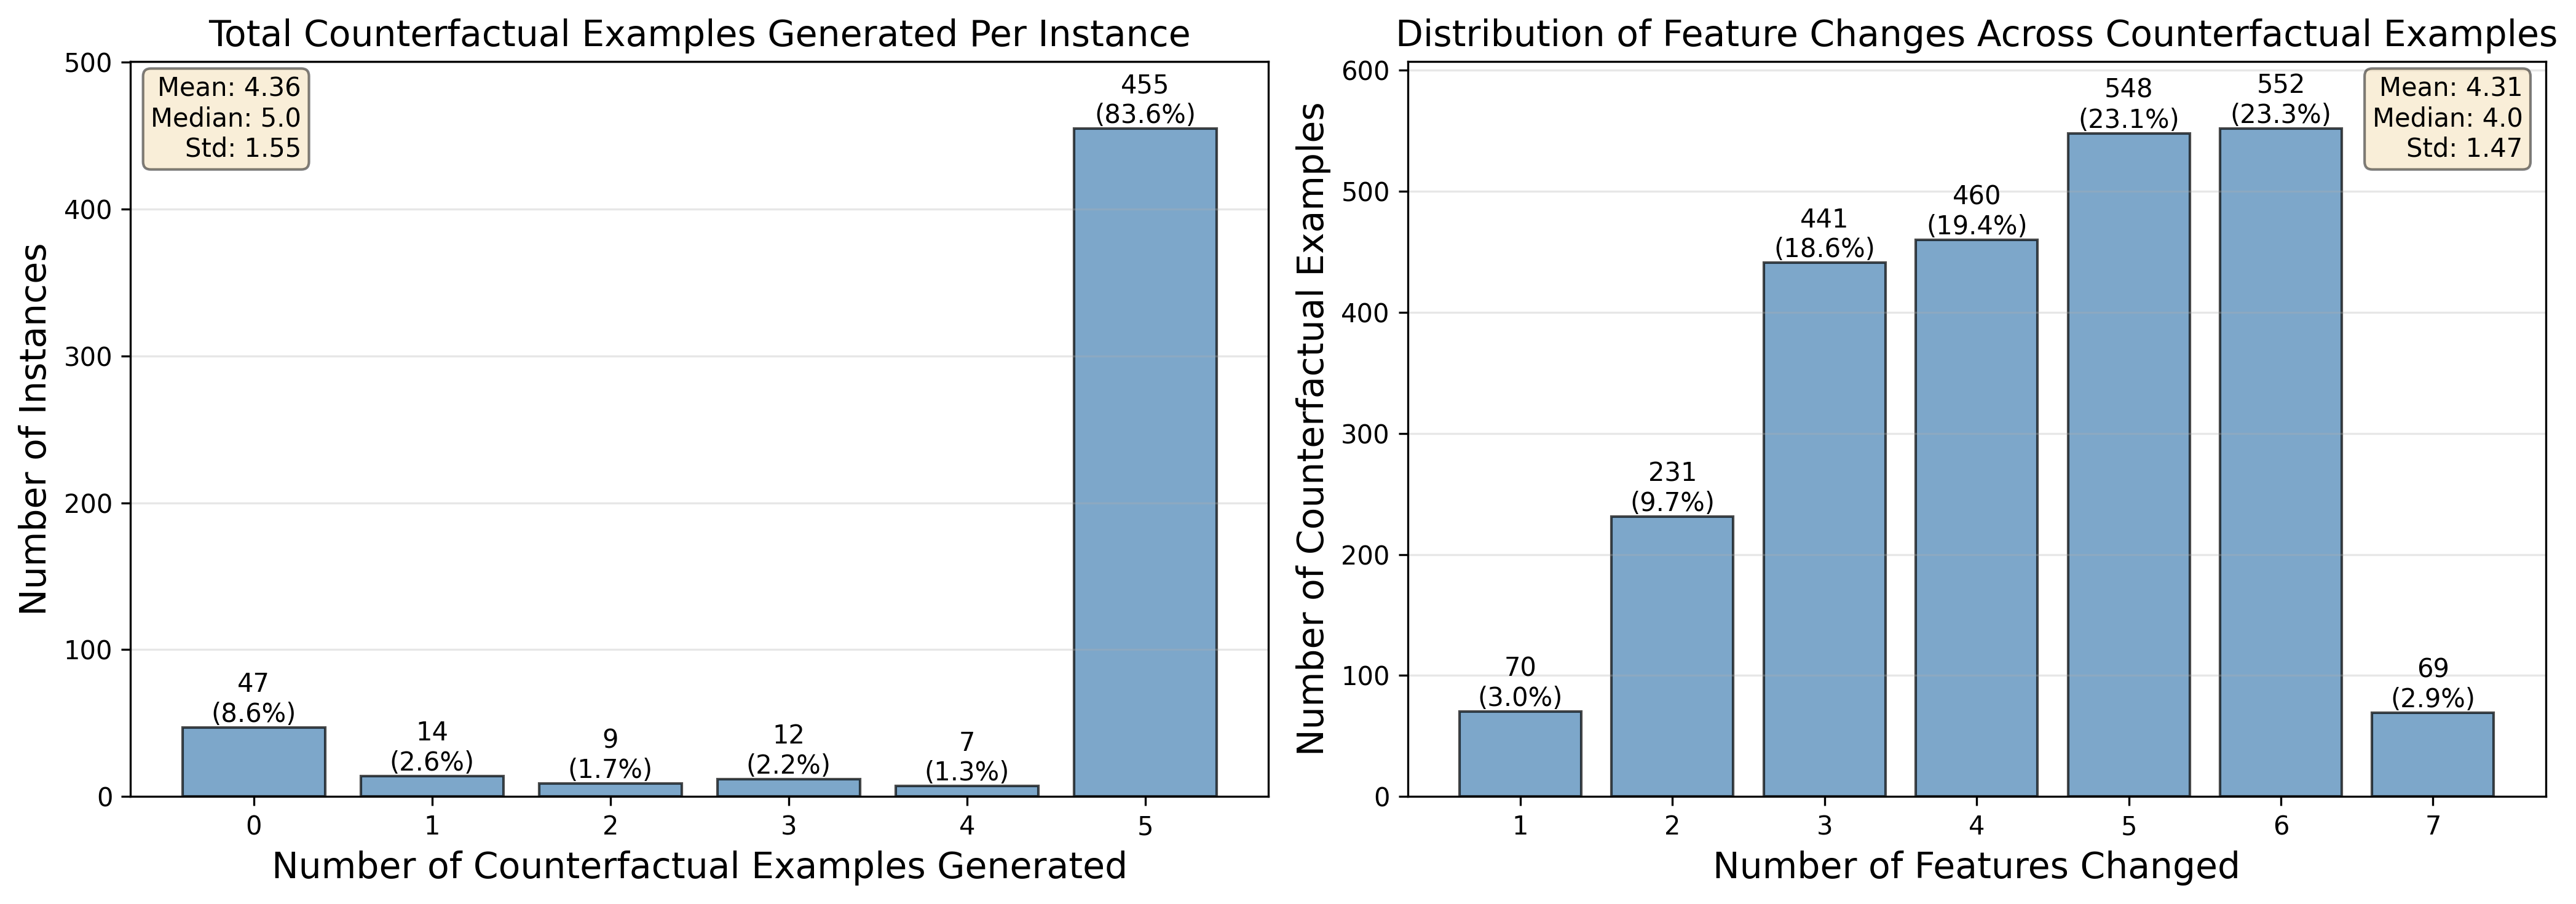
\includegraphics[width=1.0\textwidth]{figures/XAI/dementia_classification_adni_kdtree_dice_stats.png}
    \caption{Summary of generated counterfactual examples for changing the model classification from dementia to CIND}
    \label{figure:cind_dementia_dice_stat}
\end{figure}

Analyzing the changes in the features revealed that, on average, approximately 4 out of the 11 features needed to be changed to generate valid counterfactuals. The effort required for risk intervention is moderate, with the majority of counterfactual examples generated by modifying between 3 and 6 features. A minimal percentage of examples required altering only 1 feature (3\%) or up to 7 features (2.9\%). Interestingly, no counterfactual examples required changes of more than 7 features. The counterfactual explanation of the NACC cross-center validation dataset, presented in Figure~\ref{figure:dice-nacc-task2-apdx} in the appendix, resulted in similar outcomes.

The bar chart in Figure~\ref{figure:cind_dementia_dice_feature_importance} presents the frequency of changes in each feature to generate counterfactual examples. Functional activities related to daily living were the most frequently modified features to reverse the risk of dementia. The top five features are preparing balanced meals (MEALPREP, 61\%), tracking current events (EVENTS, 58\%), playing games of skill (GAMES, 54\%), shopping (SHOPPING, 54\%), and traveling (TRAVEL, 52\%). In contrast, demographics and other factors were less important, with energy levels (ENERGY), appetite changes (APP), and primary language (PRIMLANG) showing low change frequencies of 9\%, 7\%, and 2\%, respectively. Table~\ref{table:cfe-adni-task2-apdx} in the appendix presents counterfactual examples generated for a random subject classified as dementia to reverse the estimated outcome to CIND.

\begin{figure}[ht]
    \centering
    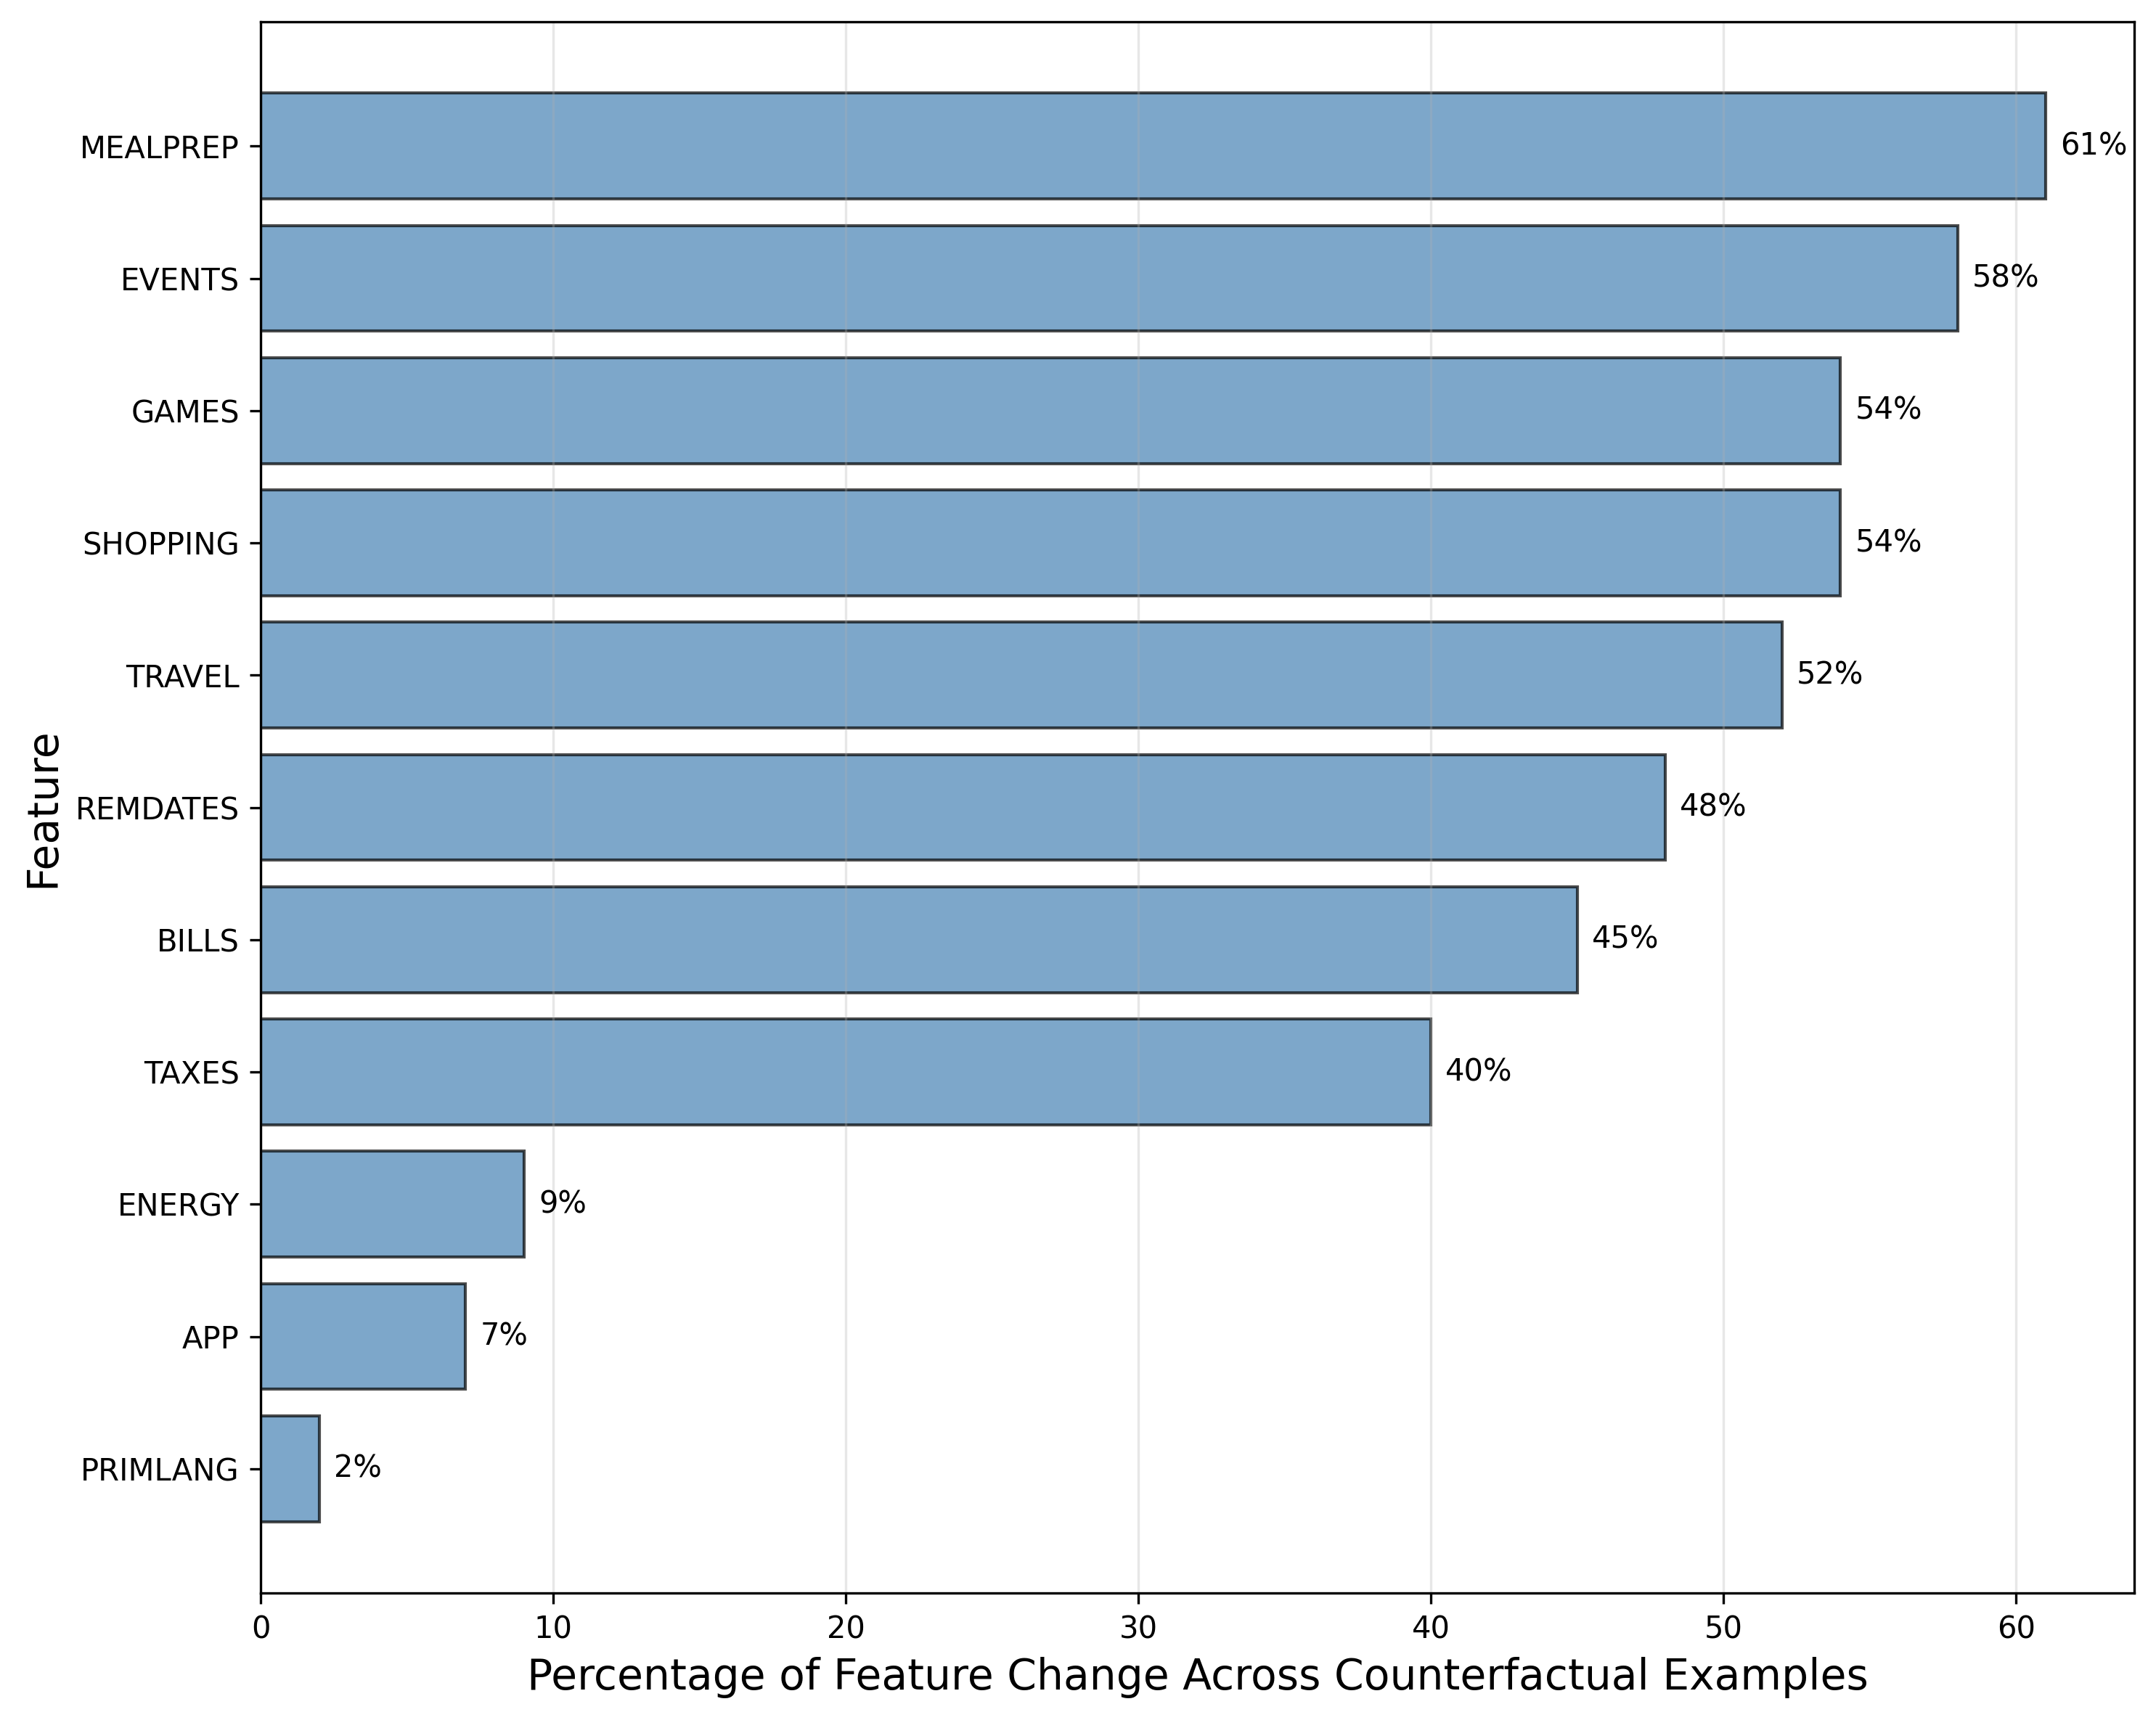
\includegraphics[width=1.0\textwidth]{figures/XAI/dementia_classification_adni_kdtree_dice_global_importance.png}
    \caption{Feature importance ranking based on counterfactual explanations for the CIND vs. dementia classification task}
    \begin{minipage}{\textwidth}
      \footnotesize The features are ranked based on the percentage of times they were modified to generate valid counterfactual examples. The rank highlights the most critical features for risk intervention.
    \end{minipage}
    \label{figure:cind_dementia_dice_feature_importance}
\end{figure}

\section{Future Cognitive Status Prediction Results}
This section presents the results for the second research objective, which focuses on developing cost-effective models to predict future cognitive status five years in advance. The same methodological steps were followed for feature selection, data resampling, model tuning and selection, and external validation. The section provides results for the normal cognition (NC) vs. cognitive impairment (CI) prediction task and the cognitive impairment but not dementia (CIND) vs. dementia prediction task.

\subsection{Feature Selection Results}
The results of the feature selection for the two cognitive status prediction tasks are presented in this subsection. The proposed feature selection method was evaluated against the baseline and the Boruta method by analyzing the performance and efficiency of the RF model and the degree of class overlap obtained from each method.

\subsubsection{Feature Selection Results for the Future NC vs. CI Prediction Task}

The feature selection evaluation was first conducted for the NC vs. CI prediction task. The comparison results for this prediction task are summarized in Table~\ref{table:fs-task3}. The RF model trained on all 66 baseline features achieved the highest G-mean (0.775), but also had the highest F1 class overlap score (0.961) and the lowest fitness score (0.646).

\begin{table}[!ht]
    \centering
    \caption{Comparison of feature selection methods for the future NC vs. CI prediction task}
    \begin{tabular}{|c|c|c|c|c|}
    \hline
        Method & Number of Features & G-mean & Fitness Score & F1 \\ \hline
        Baseline & 66 & 0.775 & 0.646 & 0.961 \\ \hline
        Boruta & 14 & 0.765 & 0.769 & 0.875 \\ \hline
        \textbf{Proposed Method} & \textbf{9} & \textbf{0.749} & \textbf{0.768} & \textbf{0.844} \\ \hline
        \multicolumn{5}{p{400pt}}{\footnotesize \hl{F1: Fisher's discriminant ratio (feature overlap measure), Fitness Score: combined score balancing performance and feature reduction, G-mean: geometric mean score.}}
    \end{tabular}
    \label{table:fs-task3}
\end{table}

The proposed method selected a minimal subset of only nine features. This was a more significant reduction than that of the Boruta method, which selected 14 features. As a result, the fitness score of the proposed method (0.768) was the highest among other methods. However, the nine selected features resulted in the lowest G-mean (0.749), which is 1.6 and 2.6 percentage points lower than the Boruta method and the baseline, respectively. This drop in RF model performance is compensated by the reduction in F1 class overlap score (0.844) and the increase in model training efficiency, which is approximately three times faster than the baseline.

Since the features selected by the proposed method resulted in the lowest RF performance, the features selected by the three methods were also tested using logistic regression LR and SVM. This is to analyze how the selected features perform across different models. The G-mean results of this analysis are presented in Table~\ref{table:fs-task3-more-models}. It can be observed that the baseline performance is the highest across all three models. However, a key finding is that the G-mean scores of the features selected by the proposed method are higher in the LR and SVM models compared to the RF model. The performance of these two models (LR and SVM) was comparable to the performance of the corresponding models trained on the 14 features selected by the Boruta method.

\begin{table}[!ht]
    \centering
    \caption{Comparison of feature selection methods in the future NC vs. CI prediction task based on G-mean performance across different models}
    \begin{tabular}{|c|c|c|c|c|}
    \hline
        Method & RF (G-mean) & LR (G-mean) & SVM (G-mean) \\ \hline
        Baseline (66 features) & 0.775 & 0.772 & 0.766 \\ \hline
        Boruta (14 features) & 0.765 & 0.759 & 0.763 \\ \hline
        Proposed Method (9 features) & 0.749 & 0.759 & 0.763 \\ \hline
        \multicolumn{4}{p{400pt}}{\footnotesize \hl{G-mean: geometric mean score, LR: logistic regression, RF: random forest, SVM: support vector machines.}}
    \end{tabular}
    \label{table:fs-task3-more-models}
\end{table}

From this supplementary analysis, it is clear that the proposed method is successful in finding the most minimal set of features that can reduce the complexity of the data and also improve the computational speed of the model. More importantly, the selected features generalize well when used with different classification algorithms.

The nine features that were selected by the proposed method for the NC vs. CI prediction task are listed in Table~\ref{table:features-task3}. The feature subset is composed of four categories of accessible data. Similarly to the previous classification tasks, this list is also heavily composed of IADL assessments from the FAQ, which account for 5 of the 9 features. The remaining items include demographic, memory complaint, and neuropsychiatric features. 

\begin{table}[h!]
\centering
\caption{List of selected features for the future NC vs. CI prediction task}
\label{table:features-task3}
\begin{tabular}{ccc}
\toprule
\textbf{Feature Code} & \textbf{Feature Description} & \textbf{Feature Category} \\
\midrule
NACCAGE & Age & Demographics \\
SEX & Sex & Demographics \\
MEMPROB & Subject reported memory problem & GDS \\
BILLS & Pay bills and track spending & FAQ \\
TAXES & Assemble tax records & FAQ \\
SHOPPING & Shop alone for necessities & FAQ \\
REMDATES & Remember dates and appointments & FAQ \\
TRAVEL & Travel out of neighborhood & FAQ \\
IRR & Irritability or lability in the last month & NPI-Q \\
\bottomrule
\end{tabular}
\end{table}

A comparison with the 12-feature set selected for the NC vs. CI classification task (Table~\ref{table:features-task1}) shows common selected features. Eight features are identical between both tasks, including NACCAGE, SEX, MEMPROB, and all five selected FAQ items. It should be noted that for this 5-year prediction task, the method did not select GAMES, EVENTS, and PAYATTN. It also selected IRR (irritability or lability) from the NPI-Q instead of ANX (anxiety). This results in a smaller, more focused set of features for the more difficult task of predicting future cognitive status.

\subsubsection{Feature Selection Results for the Future CIND vs. Dementia Prediction Task}
This subsection provides the results of the feature selection for the future CIND vs. dementia prediction task. Compared to the other classification and prediction tasks, this task is more challenging because it distinguishes the severity of cognitive impairment at five years in the future. The comparative results for this task are provided in Table~\ref{table:fs-task4}.

\begin{table}[!ht]
    \centering
    \caption{Comparison of feature selection methods for the future CIND vs. dementia prediction task}
    \begin{tabular}{|c|c|c|c|c|}
    \hline
        Method & Number of Features & G-mean & Fitness Score & F1 \\ \hline
        Baseline & 67 & 0.755 & 0.629 & 0.969 \\ \hline
        Boruta & 14 & 0.738 & 0.747 & 0.869 \\ \hline
        \textbf{Proposed Method} & \textbf{10} & \textbf{0.711} & \textbf{0.734} & \textbf{0.848} \\ \hline
        \multicolumn{5}{p{400pt}}{\footnotesize \hl{F1: Fisher's discriminant ratio (feature overlap measure), Fitness Score: combined score balancing performance and feature reduction, G-mean: geometric mean score.}}
    \end{tabular}
    \label{table:fs-task4}
\end{table}

The results show a pattern similar to that observed in the NC vs. CI prediction task. The baseline model achieved the highest G-mean (0.755), but had the lowest fitness score (0.629) and the highest F1 class overlap score (0.969). The proposed method identified a subset of ten features out of 67 features. This was smaller than the 14 features selected by the Boruta method. This set of 10-features also achieved the lowest F1 class overlap score (0.848), indicating that it was the most effective method to reduce the high complexity of this task.

In this prediction task, the features selected by the Boruta method resulted in a higher G-mean (0.738) than the proposed method's (0.711). Therefore, the Boruta method achieved the highest fitness score (0.747) in this task. However, the proposed method selected the smallest set of features and was the most cost-effective in terms of computation, with a training speed 2.9 times faster than the baseline. Additionally, its fitness score of 0.734 was significantly better than the baseline. This shows that the proposed feature selection method is able to find a strong balance between simplicity and performance even in the most difficult prediction task.

To further support this claim, the performance of the selected features of the three methods was evaluated using two more classifiers (LR and SVM) in addition to RF. The comparison of the G-mean of the three models is presented in Table~\ref{table:fs-task4-more-models}. The results are similar to those of the NC vs. CI prediction task, which can be seen in Table~\ref{table:fs-task3-more-models}. The analysis revealed that the baseline continually performs the best in all three models. However, it can be observed that the performance of the LR and SVM models trained on the ten features selected by the proposed method shows a significant increase compared to the RF performance. The G-mean scores of these two models were slightly higher than the corresponding LR and SVM models based on the Boruta method. This finding demonstrates that the proposed method can select a set of features that can produce comparable performance across different models.

\begin{table}[!ht]
    \centering
    \caption{Comparison of feature selection methods in the future CIND vs. dementia prediction task based on G-mean performance across different models}
    \begin{tabular}{|c|c|c|c|c|}
    \hline
        Method & RF (G-mean) & LR (G-mean) & SVM (G-mean) \\ \hline
        Baseline (67 features) & 0.755 & 0.765 & 0.771 \\ \hline
        Boruta (14 features) & 0.738 & 0.76 & 0.756 \\ \hline
        Proposed Method (10 features) & 0.711 & 0.761 & 0.758 \\ \hline
        \multicolumn{4}{p{400pt}}{\footnotesize \hl{G-mean: geometric mean score, LR: logistic regression, RF: random forest, SVM: support vector machines.}}
    \end{tabular}
    \label{table:fs-task4-more-models}
\end{table}

The subset of features selected by the proposed method is provided in Table~\ref{table:features-task4}. Similar to the other tasks, the list is dominated by the IADL assessments from the FAQ, which contribute 7 of the 10 features. The remaining features are the body mass index and two GDS items that survey problems with memory and energy level. More details of the selected features and their correlation results can be found in section \ref{sec:feature-selection-apdx} in the appendix.

\begin{table}[h!]
\centering
\caption{List of selected features for the future CNID vs. dementia prediction task}
\label{table:features-task4}
\begin{tabular}{ccc}
\toprule
\textbf{Feature Code} & \textbf{Feature Description} & \textbf{Feature Category} \\
\midrule
NACCBMI & Body Mass Index (\acrshort{BMI}) & Physical Assessment \\
MEMPROB & Subject reported memory problem & GDS \\
ENERGY & Do you feel full of energy? & GDS \\
BILLS & Pay bills and track spending & FAQ \\
TAXES & Assemble tax records & FAQ \\
SHOPPING & Shop alone for necessities & FAQ \\
MEALPREP & Prepare a balanced meal & FAQ \\
EVENTS & Keep track of current events & FAQ \\
REMDATES & Remember dates and appointments & FAQ \\
TRAVEL & Travel out of neighborhood & FAQ \\
\bottomrule
\end{tabular}
\end{table}


\subsection{Data Resampling Results}

\label{sec:resampling_results_ro2}
This section details the data resampling results related to the second research objective, which focuses on the 5-year future prediction of cognitive impairment. As reflected in the training datasets, the prediction of the future cognitive status is an inherently more complex problem. Therefore, applying the systematic data resampling was necessary to address the significant class imbalance and overlap challenges and to develop accurate and well-balanced prediction models. The distribution of the target classes in the NACC UDS and ADNI datasets is provided in Figure~\ref{fig:nacc-data-stat} and Figure~\ref{fig:adni-data-stat} in the appendix.

\subsubsection{Data Resampling Results for the Future NC vs. CI Prediction Task}
\label{sec:resampling_future_nc_ci}
The training dataset for the future NC vs. CI prediction task was first examined. It presented a slight class imbalance with an IR of 1.18, where the CI class was the minority. However, a high degree of data complexity was noticeable. The instance-level class overlap (kDN) score was 0.274, and the structural class overlap (N1) was particularly high at 0.389. The analysis of borderline instances showed that 26\% of the minority class (CI) and 31\% of the majority class (NC) resided in these overlapped regions.

To handle this high data complexity, the ENN + \acrshort{BorderlineSMOTE} strategy was selected by the decision algorithm (Algorithm \ref{alg:data-resampling}). The ENN method was first utilized to remove noisy instances. Since the minority class is less represented on the decision boundary, BorderlineSMOTE is used to carefully add synthetic minority class examples in this critical region. The impact of this strategy on the RF model was compared with the baseline and other data resampling methods. The comparison results are presented in Table~\ref{table:future_nc_ci_resampling}. Figure~\ref{figure:future_nc_ci_resampling_perf} provides a visual presentation of the results.

\begin{table}[!ht]
    \centering
    \caption{Performance comparison of resampling methods for the future NC vs. CI prediction task using a random forest model}
    \begin{tabular}{|c|c|c|c|c|c|}
    \hline
        Method & G-mean & Recall (NC) & Recall (CI) & kDN & N1 \\ \hline
        Baseline & 0.749 & \textbf{0.870} & 0.644 & 0.274 & 0.389 \\ \hline
        ROS & \makecell{0.749 \\ {\small \hl{(p = 0.972)}}} & 0.853 & 0.658 & 0.272 & 0.385 \\ \hline
        RUS & \makecell{0.752 \\ {\small \hl{(p = 0.175)}}} & 0.845 & 0.669 & 0.229 & 0.365 \\ \hline
        SMOTE & \makecell{0.751 \\ {\small \hl{(p = 0.135)}}} & 0.860 & 0.656 & 0.267 & 0.446 \\ \hline
        \makecell{\textbf{ENN +} \\ \textbf{BorderlineSMOTE}} & \makecell{\textbf{0.752} \\ {\small \hl{(p = 0.343)}}} & 0.812 & \textbf{0.697} & \textbf{0.018} & \textbf{0.158} \\ \hline
        \multicolumn{6}{p{400pt}}{\footnotesize \hl{G-mean: geometric mean score, kDN: k-disagreeing neighbors (instance-level class overlap), N1: structural class overlap, Recall: per-class recall.}}
    \end{tabular}
    \label{table:future_nc_ci_resampling}
\end{table}

\begin{figure}[ht]
\centering
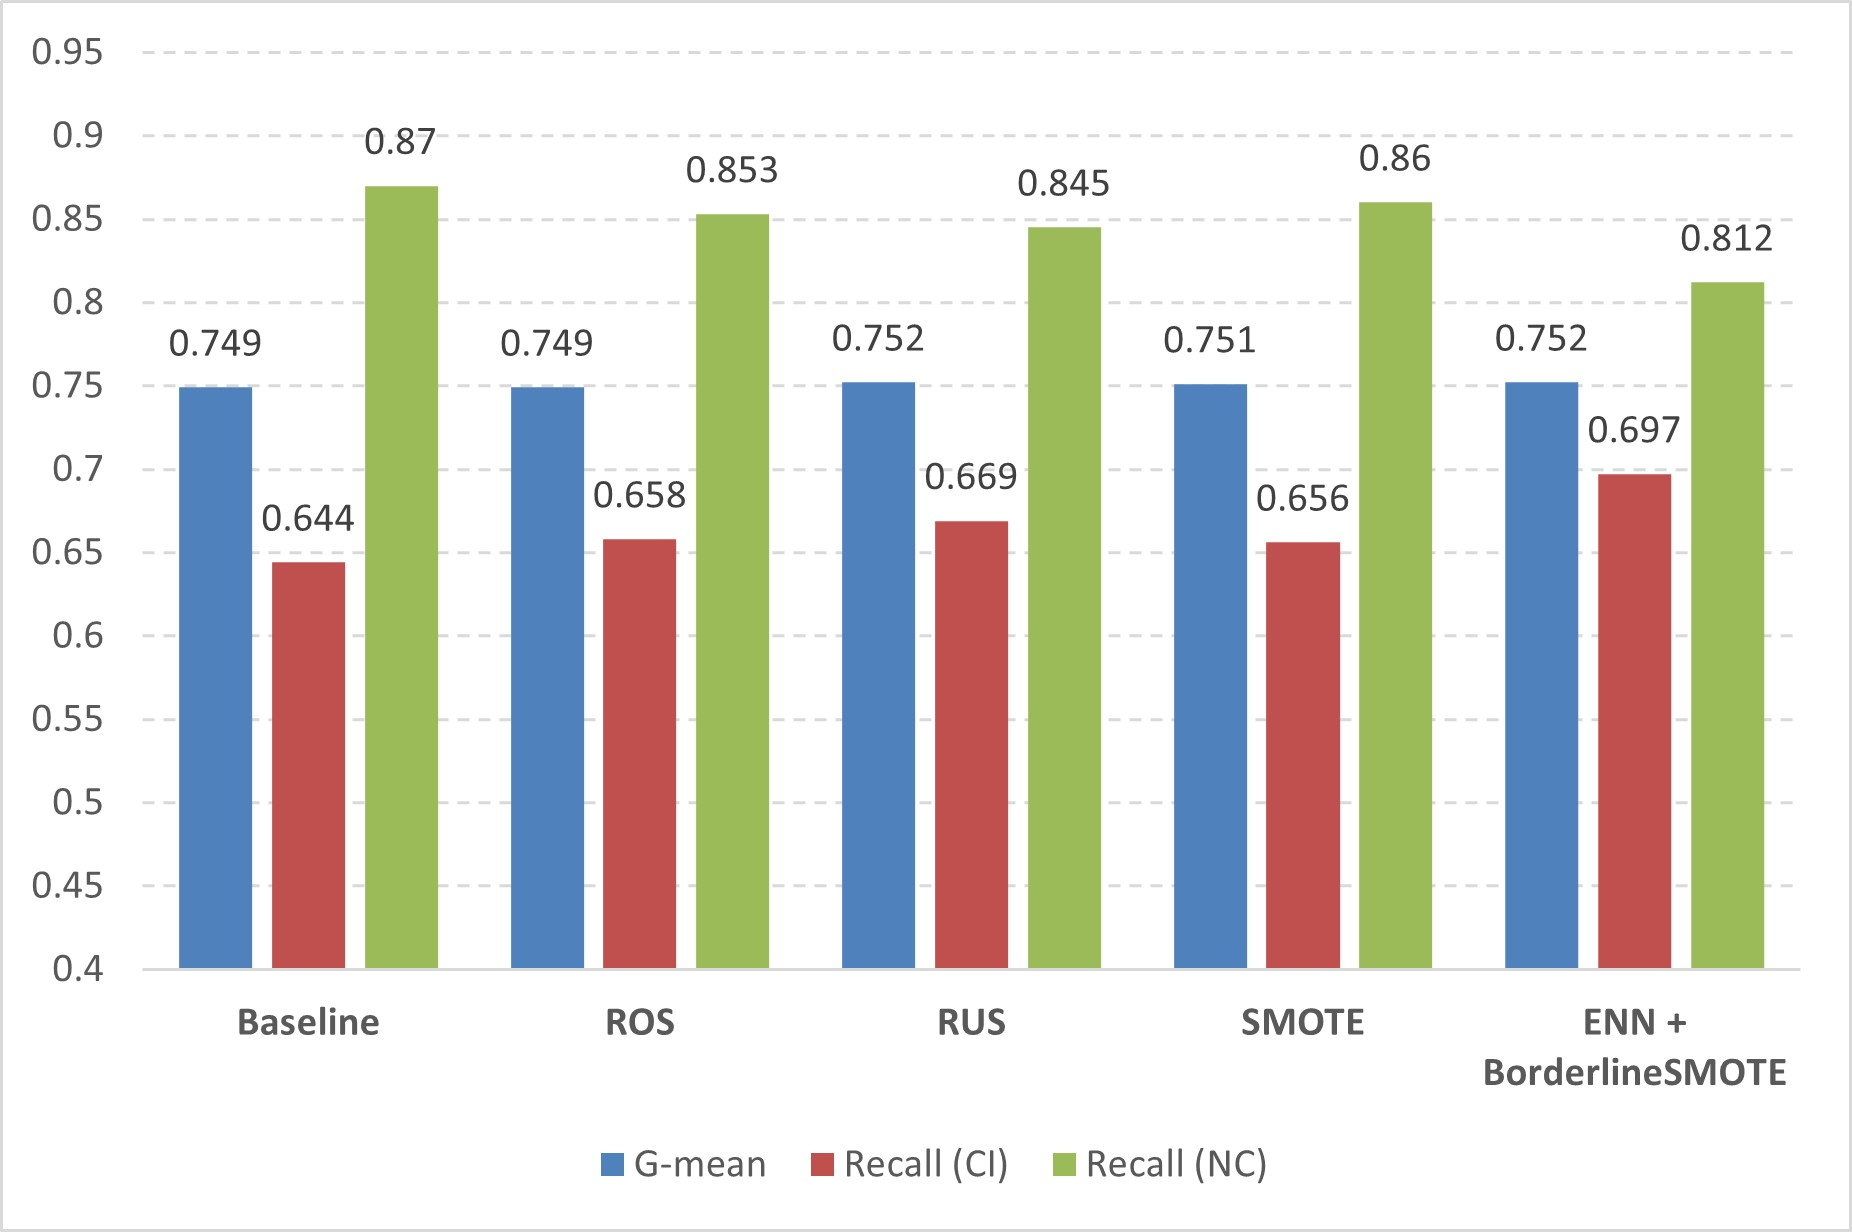
\includegraphics[width=1\textwidth]{figures/data-resampling-task3.jpg}
\caption{Model performance comparison of data resampling methods for the future NC vs. CI prediction task}
\label{figure:future_nc_ci_resampling_perf}
\end{figure}

The baseline performance, as shown in Table~\ref{table:future_nc_ci_resampling}, was heavily affected by the data complexity. The model struggled to identify the minority CI class, resulting in a low recall of 0.644. Standard methods like ROS and SMOTE did not result in any significant improvement. A key observation is that SMOTE worsened structural class overlap (N1 increased to 0.446) and provided no noticeable improvement to G-mean or recall.

The selected ENN + BorderlineSMOTE method achieved the highest balanced performance with a G-mean of 0.752. The reduction in class overlap might have allowed the RF model to learn a better decision boundary, which is reflected in the significant increase in the minority CI class recall from 0.644 to 0.697, while the NC class recall decreased from 0.870 to 0.812. \hl{The G-mean improvement of the proposed ENN + BorderlineSMOTE method over the baseline was not statistically significant (p = 0.343). This is expected, since the main benefit of the method is the reduction of class overlap rather than a direct gain in G-mean, which confirms that the synthetic data did not artificially inflate the performance.}

\subsubsection{Data Resampling Results for the Future CIND vs. Dementia Prediction Task}
\label{sec:resampling_future_cind_dem}
A similar analysis was performed for the future CIND vs. dementia prediction task. The training dataset of this task showed an IR of 1.46, with CIND as the minority class. This task presented a very high data complexity, with a kDN of 0.260 and a very high structural class overlap (N1) of 0.485. The minority class (CIND) has 39\% of its instances at the borderline compared to 26\% of the majority class (dementia) instances.

Based on this high complexity, the ENN + KMeansSMOTE method was selected by the decision algorithm (Algorithm \ref{alg:data-resampling}). This strategy was chosen to clean the noisy decision boundary with ENN, while KMeansSMOTE was applied to reinforce the sparse clusters of the minority CIND class. The performance of this method was compared with other standard techniques in Table~\ref{table:future_cind_dem_resampling}. The comparison results are also demonstrated in Figure~\ref{figure:future_cind_dem_resampling_perf}.

\begin{table}[!ht]
    \centering
    \caption{Performance comparison of resampling methods for the future CIND vs. dementia prediction task using a random forest model}
    \begin{tabular}{|c|c|c|c|c|c|}
    \hline
        Method & G-mean & Recall (Dementia) & Recall (CIND) & kDN & N1 \\ \hline
        Baseline & 0.711 & 0.770 & 0.656 & 0.260 & 0.485 \\ \hline
        ROS & \makecell{0.715 \\ {\small \hl{(p = 0.101)}}} & 0.754 & 0.678 & 0.244 & 0.469 \\ \hline
        RUS & \makecell{0.726 \\ {\small \hl{(p = 0.014)}}} & 0.723 & \textbf{0.728} & 0.250 & 0.470 \\ \hline
        SMOTE & \makecell{0.715 \\ {\small \hl{(p = 0.314)}}} & 0.758 & 0.675 & 0.238 & 0.432 \\ \hline
        \makecell{\textbf{ENN +} \\ \textbf{KMeansSMOTE}} & \makecell{\textbf{0.730} \\ {\small \hl{(p = 0.022)}}} & \textbf{0.776} & 0.688 & \textbf{0.034} & \textbf{0.161} \\ \hline
        \multicolumn{6}{p{400pt}}{\footnotesize \hl{G-mean: geometric mean score, kDN: k-disagreeing neighbors (instance-level class overlap), N1: structural class overlap, Recall: per-class recall.}}
    \end{tabular}
    \label{table:future_cind_dem_resampling}
\end{table}

\begin{figure}[H]
\centering
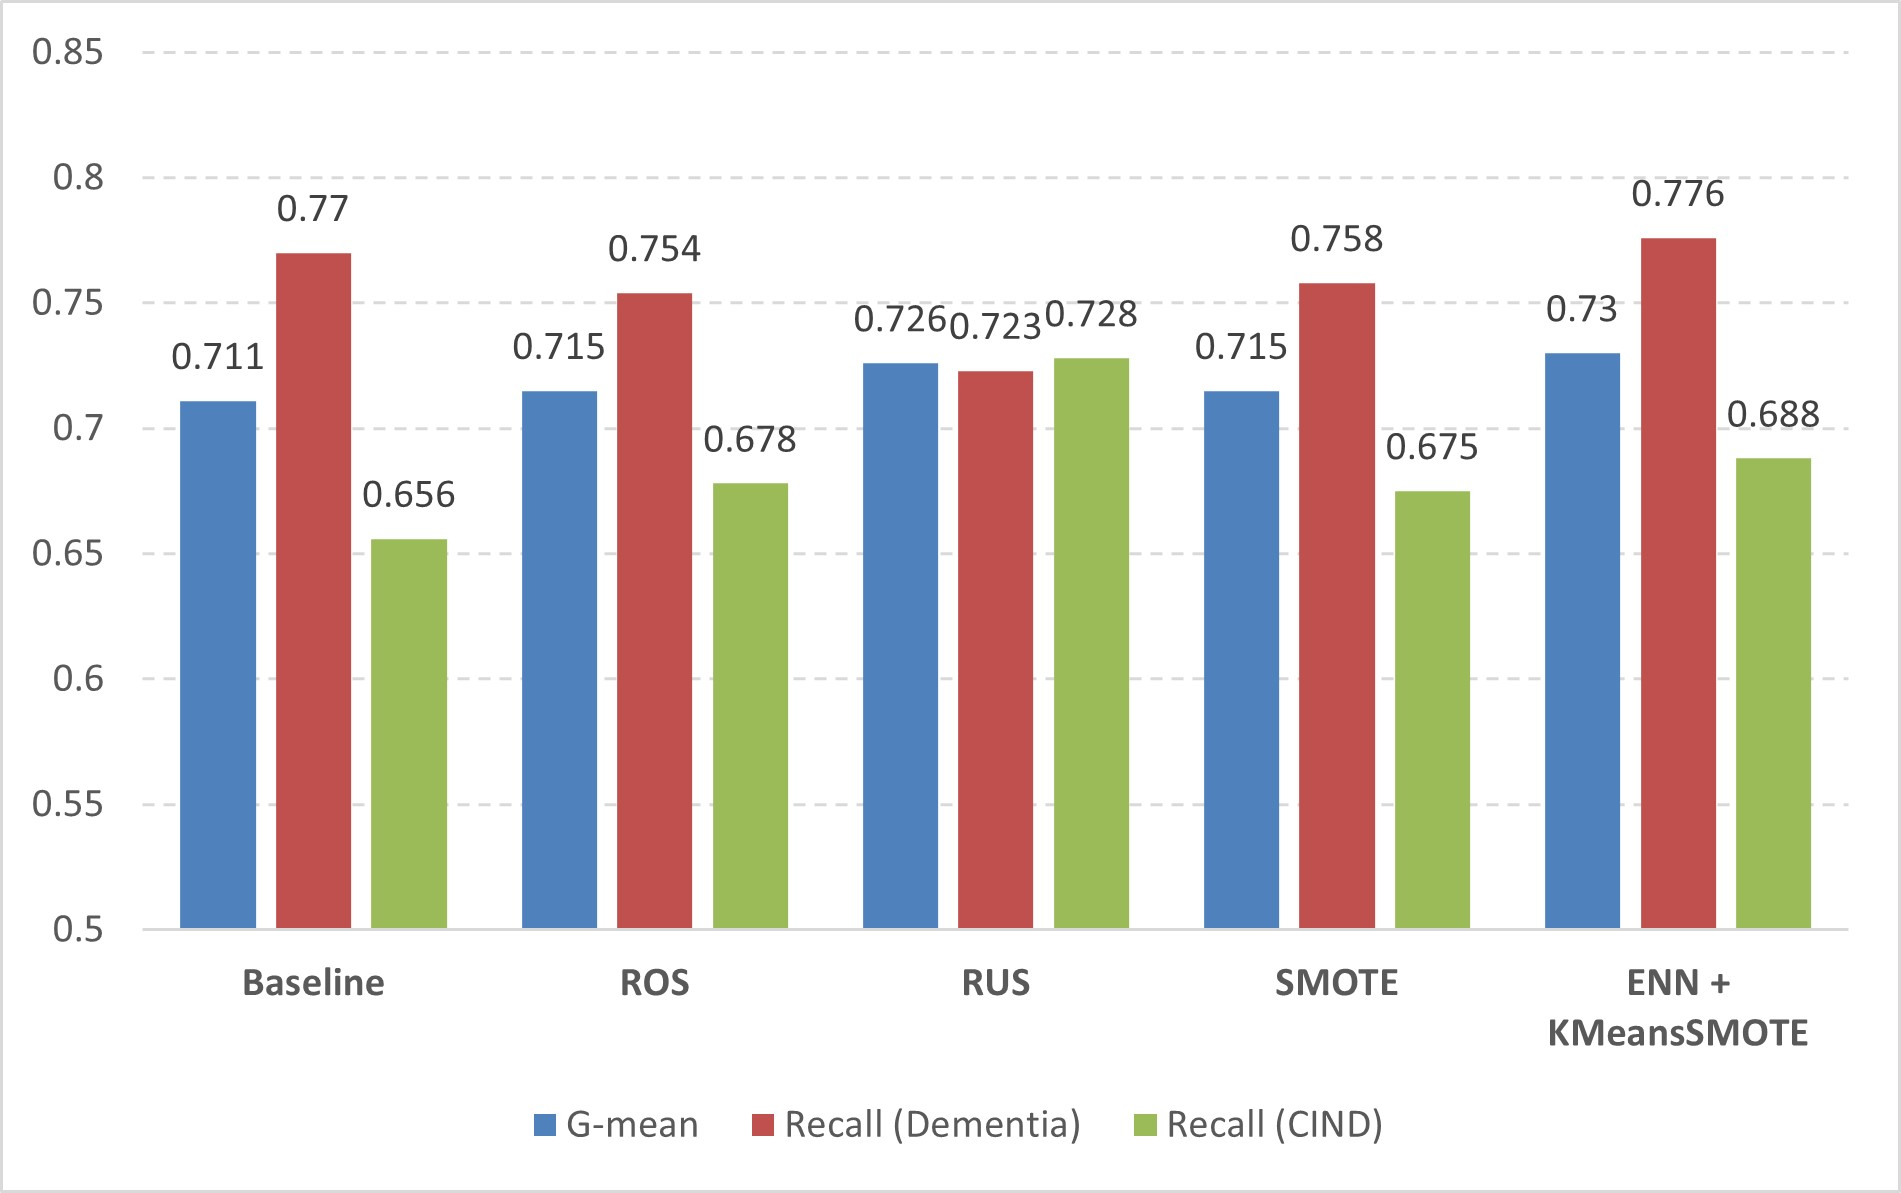
\includegraphics[width=1\textwidth]{figures/data-resampling-task4.jpg}
\caption{Model performance comparison of data resampling methods for the future CIND vs. dementia prediction task}
\label{figure:future_cind_dem_resampling_perf}
\end{figure}

The baseline model experienced classification complexity due to the high class overlap in this task. As a result, the model had a low G-mean of 0.711 and a poor recall for the minority CIND class (0.656). The RUS method reduced the density of the majority class, which slightly lowered the class overlap. This allowed the RF model to achieve the highest recall of the minority CIND class (0.728) and to improve the baseline G-mean to 0.726. However, it removed informative patterns of the dementia class, resulting in the most significant drop in dementia recall from 0.770 to 0.723. This outcome might not be acceptable, as misclassifying dementia cases could have a higher risk and cost. A similar outcome was observed in the ROS and SMOTE methods, with both methods slightly improving the baseline G-mean to 0.715.

The ENN + KMeansSMOTE method increased the G-mean to 0.730. This method was the only one that improved the recall for both classes simultaneously. \hl{This G-mean improvement over the baseline was statistically significant (p = 0.022), which supports the reliability of the proposed overlap-aware strategy.} This high performance is explained by the significant reduction in data complexity. By cleaning the data, the method improved the model's recall on the difficult minority CIND class from 0.656 to 0.688 while also slightly improving the recall on the dementia class.

In conclusion, the baseline model suffered from high class overlap in both future prediction tasks. The overlap-guided resampling methodology produced highly effective results. It successfully identified and applied hybrid techniques that reduced the data complexity and improved the model's ability to classify both classes more accurately. These results move the outcomes of this study closer to achieving the research objectives and improve the training data quality for better modeling results, which are highlighted in the next subsections.

\subsection{Model Fine-tuning and Selection Results}
Following the feature selection and data resampling stages, the hyperparameters of five classification models were optimized, and the most cost-effective model was selected. This section details the results of this process for the two tasks to predict cognitive status up to five years in the future.

\subsubsection{Model Fine-tuning and Selection Results for the Future NC vs. CI Prediction Task}
The cost-effective model selection algorithm (Algorithm \ref{alg:model-selection}) was applied to the grid search results for the five prediction models. The primary objective was to find model hyperparameters that maintain high performance while increasing efficiency. The training throughput of the LightGBM model increased by 3.59 times, and the prediction throughput showed around a three-times increase. This was done with a minor decrease in performance compared to the best-performing LightGBM model (the F1-score was dropped from 0.751 to 0.744). Similarly, substantial improvement in prediction speed was shown by the KNN model. Table~\ref{table:task3_finalists_models} summarizes the performance and efficiency metrics of the five models selected by the algorithm.

\begin{table}[!ht]
\centering
\caption{Summary of fine-tuned models for the future NC vs. CI prediction task}
\label{table:task3_finalists_models}
\newcolumntype{C}{>{\centering\arraybackslash}X}
    \begin{tabularx}{\textwidth}{|C|C|C|C|C|}
        \hline
        \textbf{Model} &
        \textbf{F1-score (95\% CI)} &
        \textbf{G-mean (95\% CI)} &
        \textbf{Training Throughput (Gain)\textsuperscript{1}} &
        \textbf{Prediction Throughput (Gain)\textsuperscript{1}} \\
        \hline
        KNN &
        0.723 ($\pm 0.002$) &
        0.750 ($\pm 0.002$) &
        $1,044,635$ $(1.03\times)$ &
        $48,105$ $(2.64\times)$ \\
        \hline
        LR &
        0.747 ($\pm 0.002$) &
        0.770 ($\pm 0.002$) &
        $819,113$ $(1.04\times)$ &
        $6,630,848$ $(1.07\times)$ \\
        \hline
        LightGBM &
        0.744 ($\pm 0.003$) &
        0.756 ($\pm 0.003$) &
        $114,209$ $(3.59\times)$ &
        $710,044$ $(2.93\times)$ \\
        \hline
        RF &
        0.750 ($\pm 0.004$) &
        0.769 ($\pm 0.004$) &
        $27,856$ $(1.05\times)$ &
        $186,313$ $(1.06\times)$ \\
        \hline
        SVM &
        0.747 ($\pm 0.003$) &
        0.768 ($\pm 0.003$) &
        $2,647$ $(1.02\times)$ &
        $20,074$ $(1.28\times)$ \\
        \hline
        \multicolumn{5}{p{400pt}}{\footnotesize \textsuperscript{1}\hl{Training throughput is reported in training samples per second, and prediction throughput in predictions per second.} Gain is calculated as the ratio of the selected model’s throughput to the benchmark model’s throughput. Values indicate the factor by which training and prediction speed have improved.}
    \end{tabularx}
\end{table}

To select a single best model for this prediction task, a final assessment was performed. The assessment compares the models according to performance, efficiency, and interpretability. Based on the results in Table~\ref{table:task3_finalists_models}, the LR model was chosen as the final model.

The LR model outperformed other models in multiple criteria. In terms of performance, the LR model was one of the best-performing models, achieving an F1-score of 0.747. This score is similar to the performance achieved by the SVM and LightGBM models. The RF model obtained a marginally better F1-score of 0.750. The KNN model continued to achieve the lowest performance as observed in the other classification tasks. With multiple models scoring high performance, efficiency was assessed to differentiate them. Superior computational speed was exhibited by the LR model, with a prediction throughput of over 6.6 million samples per second. This is extremely faster than the RF, SVM, and LightGBM models. Finally, the interpretability of the model is crucial for this study. As a linear model, LR allows for a straightforward explanation of how risk factors influence the prediction of future cognitive impairment. A significant advantage is offered by this over the complex, non-linear nature of the RF and SVM models. Therefore, the overall balance of comparable accuracy, high speed, and easy interpretability justify the selection of the LR model. Table~\ref{table:lr-fine-tune-task3-apdx} in the appendix presents the hyperparameter fine-tuning results of the LR model.

\subsubsection{Model Fine-tuning and Selection Results for the Future CIND vs. Dementia Prediction}
Similar to the previous task, the cost-effective selection algorithm was utilized to filter the models generated by the grid search hyperparameters fine-tuning. The algorithm found highly efficient hyperparameters for the RF, LightGBM, and KNN models. A particularly substantial improvement was found for the RF model, where the selected model achieved around a three-times increase in training and prediction speed compared to the benchmark model (RF model with the highest performance). This was obtained with only a marginal reduction in performance. A similar increase in training and prediction speed was observed in the LightGBM model. The LR model also saw a lower degree of increase in training and prediction speed. Table~\ref{table:task4_finalists_models} details the performance metrics and throughput gains for the five selected models.

\begin{table}[!ht]
\centering
\caption{Summary of fine-tuned models for the future CIND vs. dementia Prediction Task}
\label{table:task4_finalists_models}
\newcolumntype{C}{>{\centering\arraybackslash}X}
    \begin{tabularx}{\textwidth}{|C|C|C|C|C|}
        \hline
        \textbf{Model} &
        \textbf{F1-score (95\% CI)} &
        \textbf{G-mean (95\% CI)} &
        \textbf{Training Throughput (Gain)\textsuperscript{1}} &
        \textbf{Prediction Throughput (Gain)\textsuperscript{1}} \\
        \hline
        KNN &
        0.772 ($\pm 0.014$) &
        0.732 ($\pm 0.014$) &
        $1,003,616$ $(1.14\times)$ &
        $61,623$ $(3.15\times)$ \\
        \hline
        LR &
        0.773 ($\pm 0.011$) &
        0.757 ($\pm 0.009$) &
        $744,495$ $(1.14\times)$ &
        $5,276,181$ $(1.41\times)$ \\
        \hline
        LightGBM &
        0.770 ($\pm 0.014$) &
        0.751 ($\pm 0.012$) &
        $58,983$ $(2.67\times)$ &
        $386,914$ $(2.46\times)$ \\
        \hline
        RF &
        0.780 ($\pm 0.016$) &
        0.751 ($\pm 0.015$) &
        $17,395$ $(3.15\times)$ &
        $130,213$ $(3.00\times)$ \\
        \hline
        SVM &
        0.772 ($\pm 0.011$) &
        0.756 ($\pm 0.013$) &
        $9,608$ $(1.07\times)$ &
        $46,531$ $(1.09\times)$ \\
        \hline
        \multicolumn{5}{p{400pt}}{\footnotesize \textsuperscript{1}\hl{Training throughput is reported in training samples per second, and prediction throughput in predictions per second.} Gain is calculated as the ratio of the selected model’s throughput to the benchmark model’s throughput. Values indicate the factor by which training and prediction speed have improved.}
    \end{tabularx}
\end{table}

The LR model was subsequently selected as the most cost-effective model. This decision is explained by a balanced evaluation of three criteria. First, the LR model obtained an F1-score of 0.773. Slightly higher scores of 0.780 and 0.777 were achieved by the RF model and the LightGBM model, respectively. Second, in terms of efficiency, the LR model offers a prediction throughput of over 5.2 million samples per second, which is much faster than all other models. Finally, the transparency of the linear LR model allows a clear interpretation of predictive factors. The RF and LightGBM models are less interpretable and significantly more computationally expensive. Therefore, the LR model was again selected as the final model for this classification task because it provides a considerable balance between performance and computational efficiency, as well as easy interpretation of the prediction. The hyperparameter fine-tuning results of the LR model is presented in Table~\ref{table:lr-fine-tune-task4-apdx} in the appendix.

In summary, the application of the fine-tuning and selection methodology to the future cognitive status prediction tasks has produced similar results to the current classification tasks. For both the NC vs. CI and CIND vs. dementia prediction tasks, the LR model was identified as the most suitable candidate. These findings confirm the feasibility of using cost-effective and explainable models for predicting future cognitive decline. The following section will evaluate the generalizability of these selected models using external validation data.

\subsection{Model Performance in External Validation}
The two selected LR models for the prediction of cognitive status 5 years in the future were tested using two separate datasets to assess their generalizability. First, the models were tested on the holdout NACC cross-center testing dataset (which represents 20\% of the original data) to evaluate their performance on unseen data from different research centers. In addition, an independent external validation was performed using the ADNI dataset. Moreover, the results of the models' calibration and clinical utility evaluation in both external validation datasets were presented. The details of the validation method are described in section \ref{sec:model-validation}.

\subsubsection{External Validation Results for the Future NC vs. CI Prediction Task}
The performance of the LR model to predict the future risk of CI was analyzed across the internal and external validation datasets. A comparison of performance metrics is provided in Table~\ref{tab:future_nc_ci_results}. Additionally, the ROC curves for the three validation stages are shown in Figure~\ref{fig:future_nc_ci_roc}.

\begin{table}[!ht]
    \centering
    \caption{Performance of the selected logistic regression model in internal and external validation for the future NC vs. CI prediction task}
    \label{tab:future_nc_ci_results}
    \newcolumntype{C}{>{\centering\arraybackslash}X}
        \begin{tabularx}{\textwidth}{|c|c|C|C|}
            \hline
            \textbf{Metric} & \textbf{Internal CV} & \textbf{NACC Cross-center Validation} & \textbf{ADNI External Validation} \\
            \hline
            AUC & \makecell{0.772 \\ {\small \hl{(0.769--0.776)}}} & \makecell{0.790 \\ {\small \hl{(0.774--0.806)}}} & \makecell{0.778 \\ {\small \hl{(0.750--0.803)}}} \\ \hline
            G-mean & 0.770 & 0.787 & 0.777 \\ \hline
            Sensitivity & 0.723 & 0.721 & 0.745 \\ \hline
            Specificity & 0.820 & 0.859 & 0.810 \\ \hline
            F1-score & 0.747 & 0.772 & 0.791 \\
            \hline
             \multicolumn{4}{p{400pt}}{\footnotesize \hl{AUC: area under the curve, F1-score: harmonic mean of precision and recall, G-mean: geometric mean score, Sensitivity: recall of the CI class, Specificity: recall of the NC class.}}
        \end{tabularx}
\end{table}

\begin{figure}[ht]
    \centering
    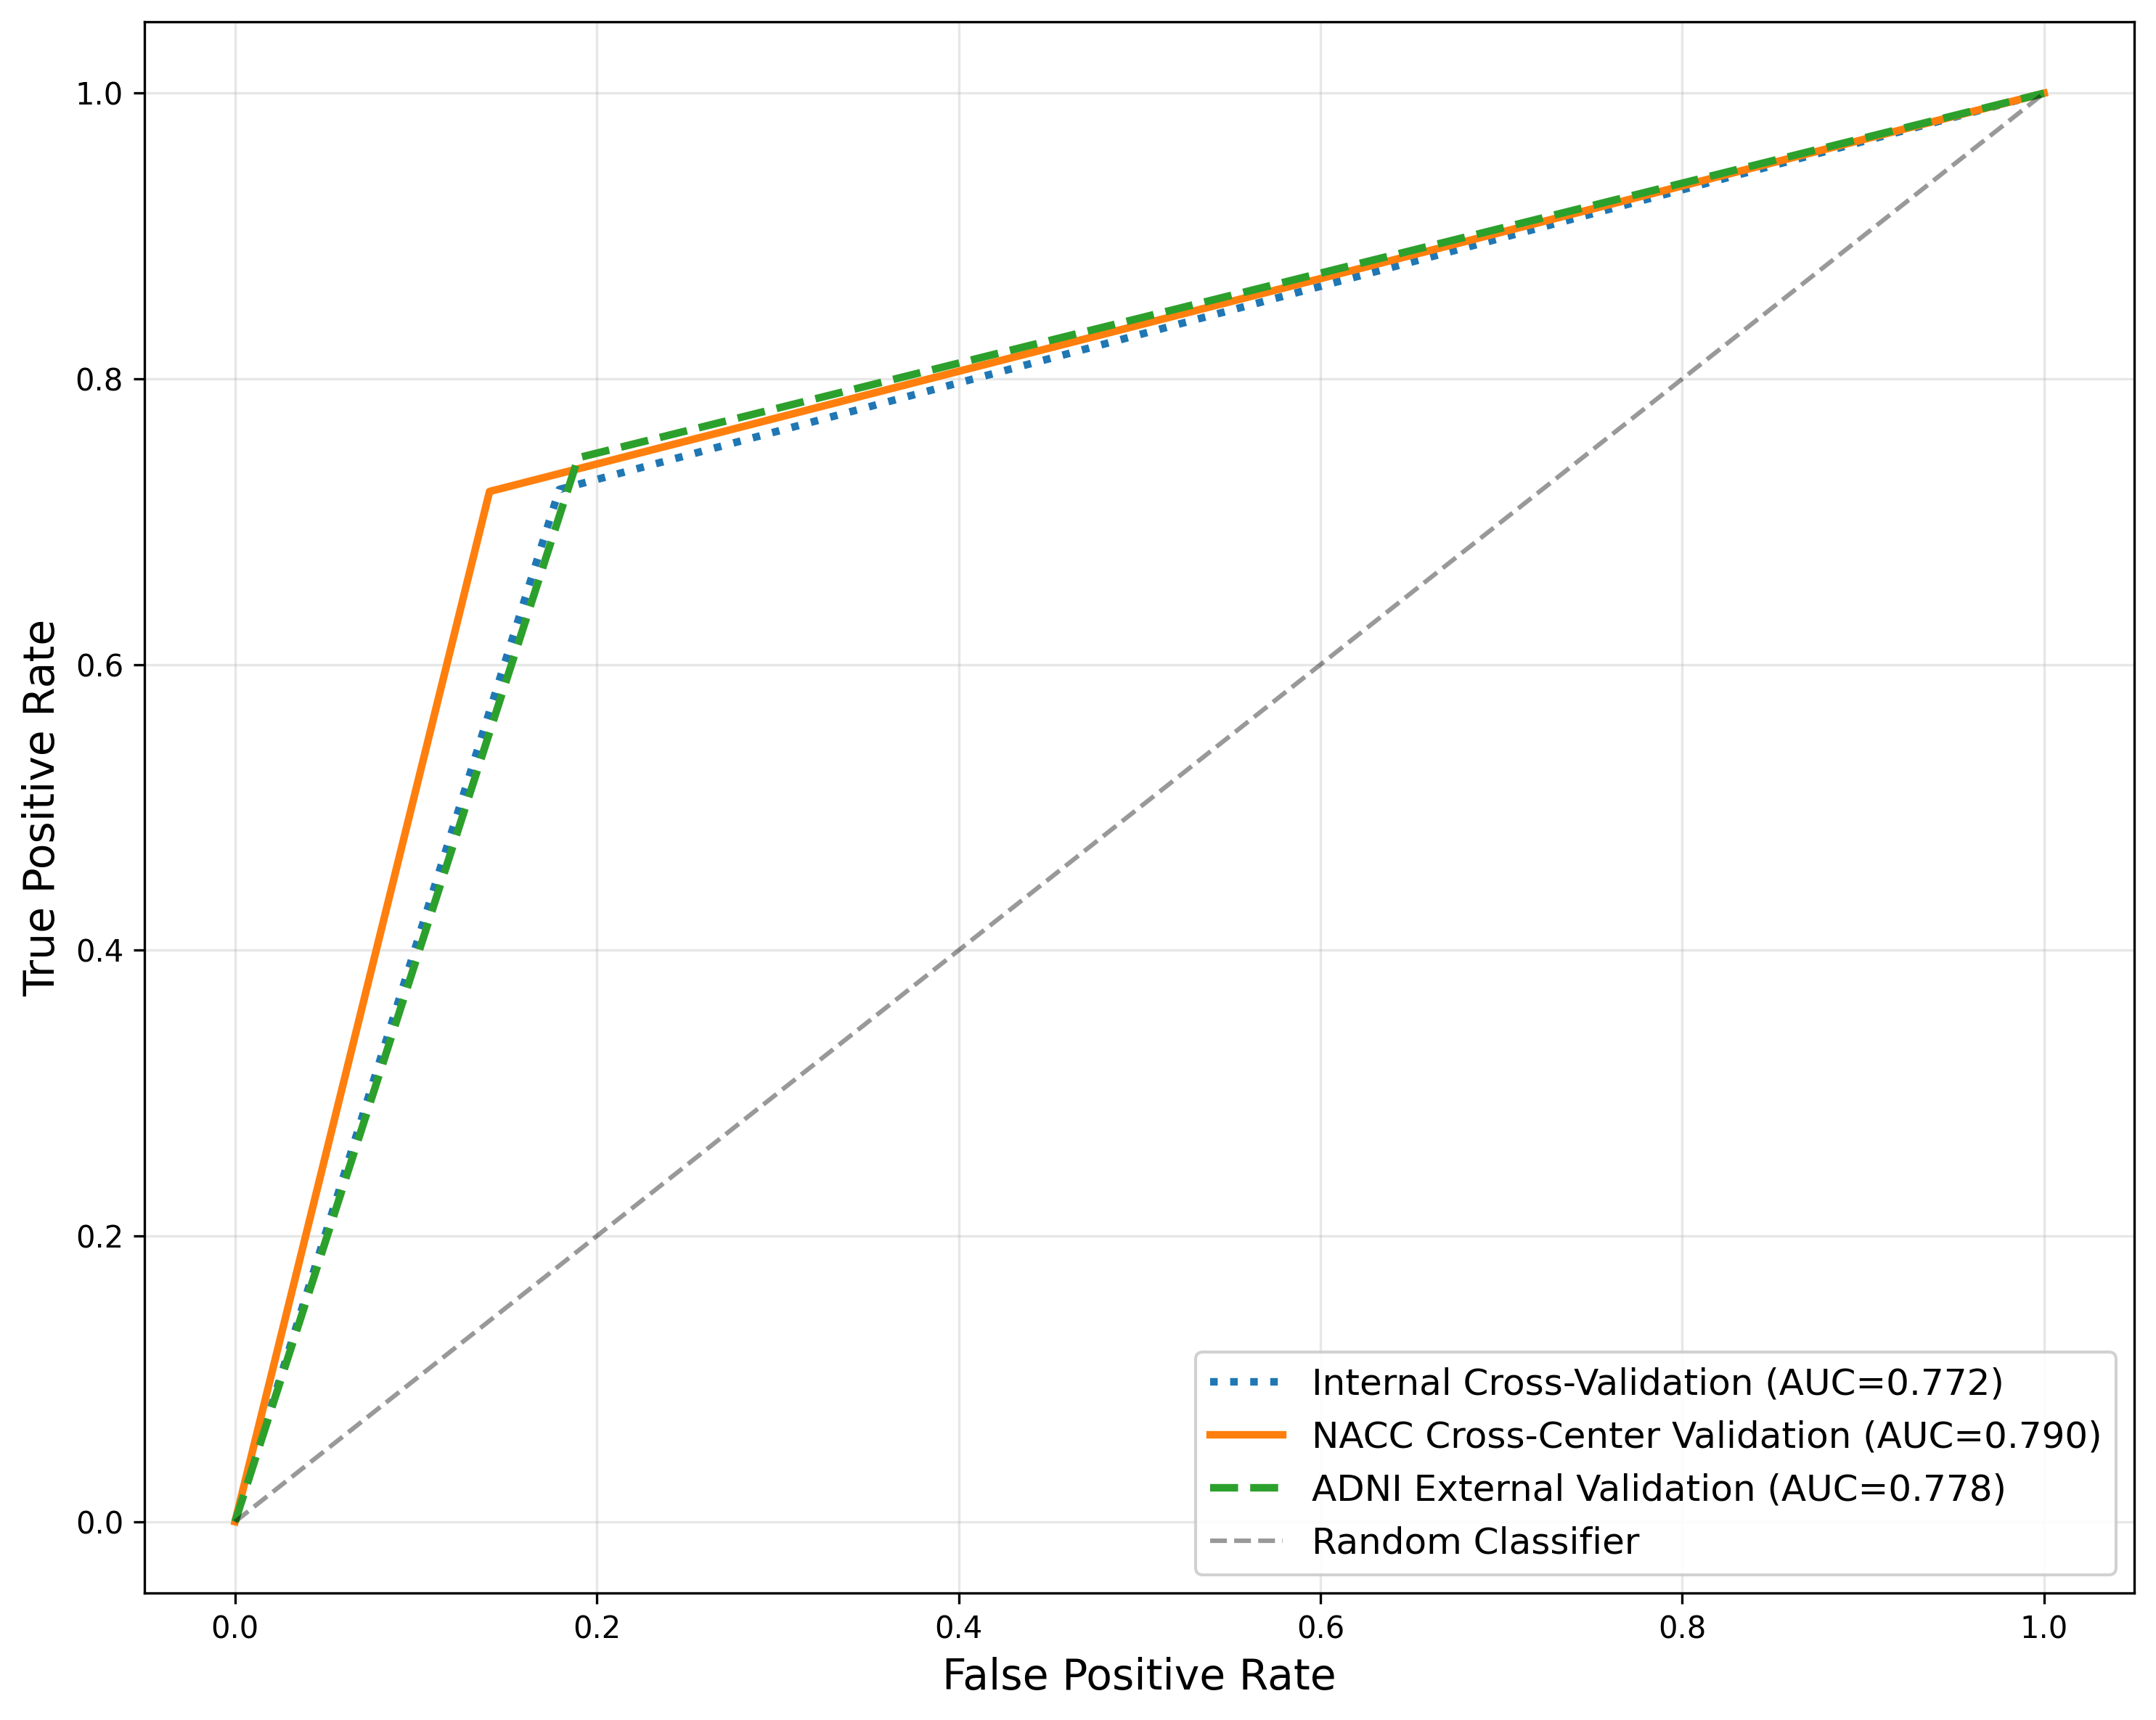
\includegraphics[width=0.7\textwidth]{figures/impaired_prediction_all_tests_roc_overlay.png}
    \caption{ROC curves comparing the performance of the logistic regression model for the future NC vs. CI prediction task}
    \begin{minipage}{\textwidth}
      \footnotesize \hl{The horizontal axis shows the false positive rate (1 -- specificity) and the vertical axis shows the true positive rate (sensitivity). Each curve represents one validation dataset.}
    \end{minipage}
    \label{fig:future_nc_ci_roc}
\end{figure}

The results of the NACC cross-center validation showed an improvement in performance compared to the internal CV. Unlike the results of the current cognitive status classification task (section \ref{sec:classification_external_validation}), the AUC score increased from 0.772 to 0.790, and the G-mean improved from 0.770 to 0.787. This improvement is attributed to the significant increase in NC recall (specificity) from 0.820 to 0.859, while the CI recall had a very minimal decrease. These findings suggest that the model was exceptionally well generalized to the unseen NACC data collected in different research centers.

The model also demonstrated high performance when applied to the ADNI dataset. The AUC score of 0.778 is very close to the internal CV score and only slightly lower than the NACC cross-center validation score. This can be observed in Figure~\ref{fig:future_nc_ci_roc} as the ADNI external validation's ROC curve is close to the other curves. Importantly, the sensitivity was 0.745 in the ADNI external validation, which outperformed the sensitivity of the other two validations. This indicates that the model is reliable in identifying cases at risk of future CI in a different clinical population. However, the model scored the lowest NC recall of 0.810 in the ADNI external validation. \hl{Both external AUC scores differed significantly from the internal CV (NACC cross-center p < 0.001, ADNI p = 0.036), although the differences were small and within an acceptable range for generalization.} Table~\ref{table:lr-complete-perf-task3-apdx} in the appendix provides extended performance metrics of the external validation results.

Calibration of the LR model was also performed to produce a reliable estimate of future CI risk. Figure~\ref{fig:future_nc_ci_calib_curve} demonstrates the calibration curves for both validation datasets. In the NACC cross-center validation, the uncalibrated model overestimated the risk at most of the interval and generated extreme probabilities close to 0 and 1. After beta calibration was applied, the distribution of the predicted probabilities was corrected with excellent intercept and slope. As a result, the ECE was significantly reduced from 0.108 to 0.023, and the Brier score improved from 0.164 to 0.148. This indicates excellent calibration and accuracy of the model's prediction.

\begin{figure}[ht]
    \centering
    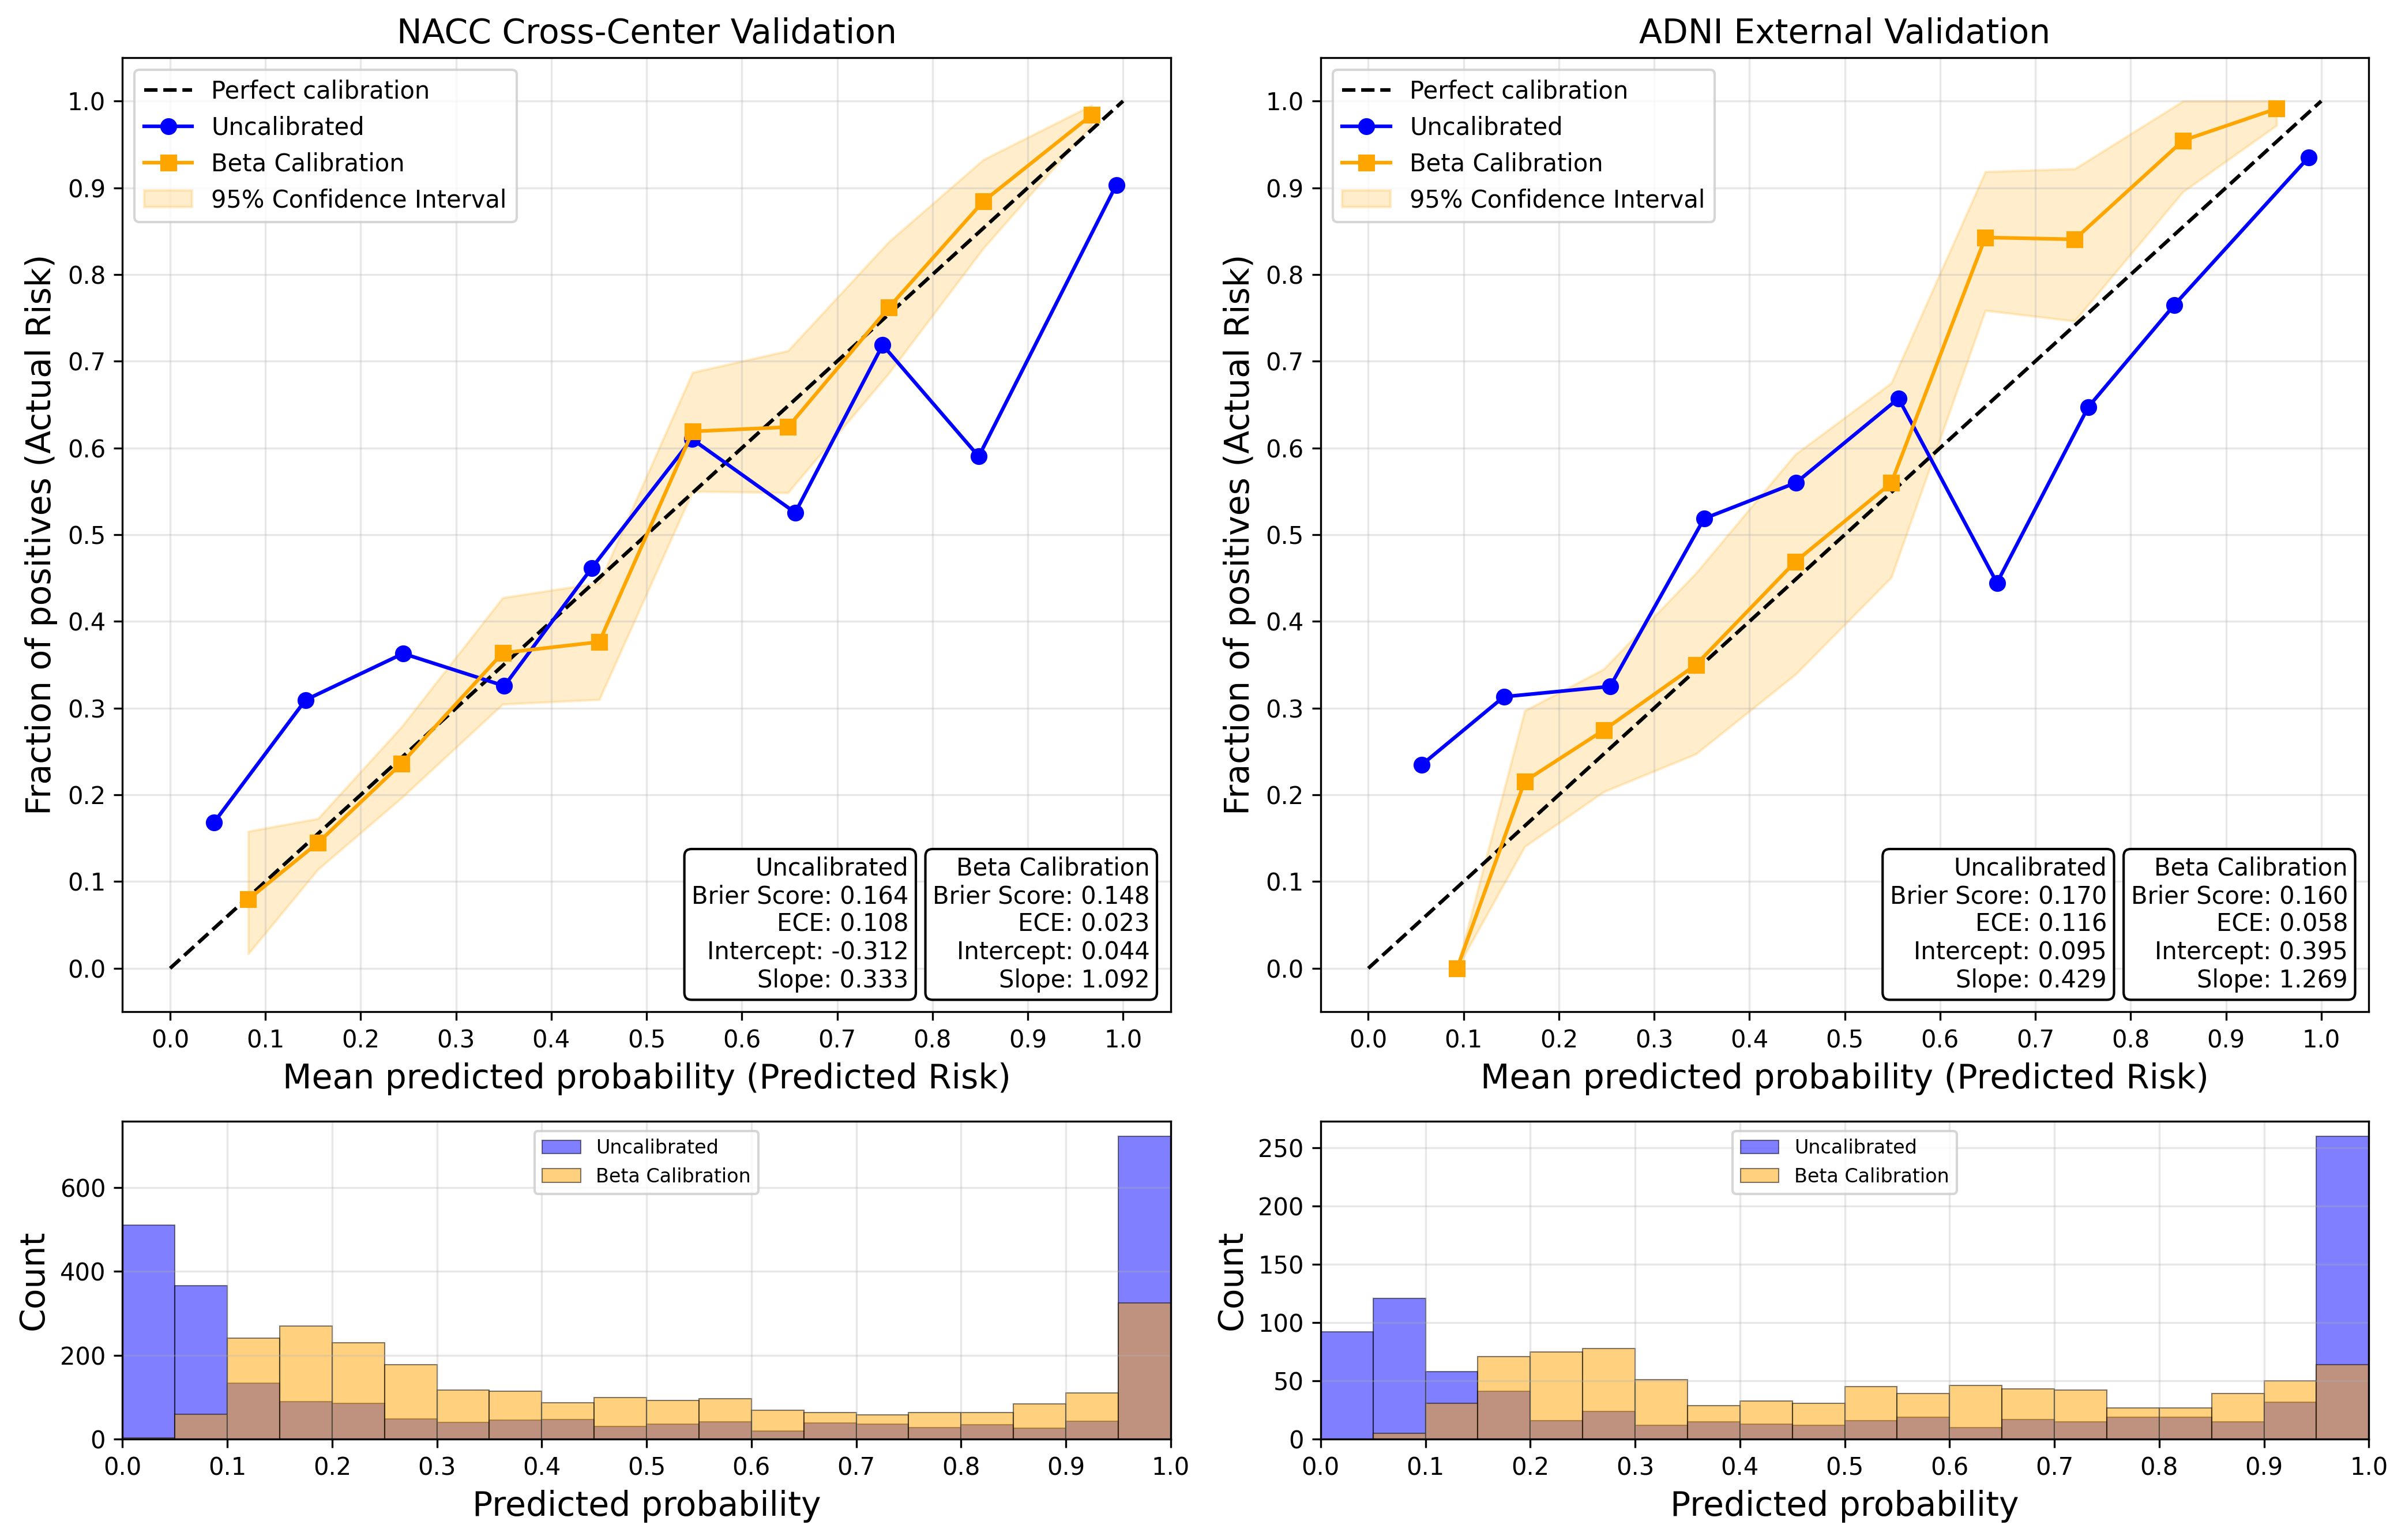
\includegraphics[width=1.0\textwidth]{figures/calibration/impaired_prediction_both_calibration_curve.png}
    \caption{Model calibration curves for the future NC vs. CI prediction task}
    \begin{minipage}{\textwidth}
      \footnotesize \hl{The horizontal axis shows the predicted probability and the vertical axis shows the observed frequency of the positive class. The diagonal line represents perfect calibration, and the curves compare the model before and after beta calibration.}
    \end{minipage}
    \label{fig:future_nc_ci_calib_curve}
\end{figure}

Similar improvements were observed in the ADNI external validation. Before calibration, the model produced extreme probabilities that did not correctly identify risk levels. The application of beta calibration successfully adjusted the spread of the predictions (slope = 1.269), although it resulted in underestimation of the CI risk in certain thresholds (intercept = 0.395). Overall, the calibration error was significantly reduced, as the ECE decreased from 0.116 to 0.058. This shows that the beta calibration method was able to successfully align the predicted probabilities with the actual results in both external validation datasets.

The excellent calibration of the LR model's predicted probabilities made the model highly valuable for clinical prediction of future CI. According to the DCA shown in Figure~\ref{fig:future_nc_ci_dca}, the model's net benefit exceeded that of the "treat all" and "treat none" strategies across a wide range of probability thresholds, specifically from 0.14 to 0.98 for the NACC cross-center validation and from 0.23 to 0.99 for the ADNI external validation. This result highlights that the LR model can provide clinical value in a wide range of risk threshold probabilities of future CI.

\begin{figure}[ht]
    \centering
    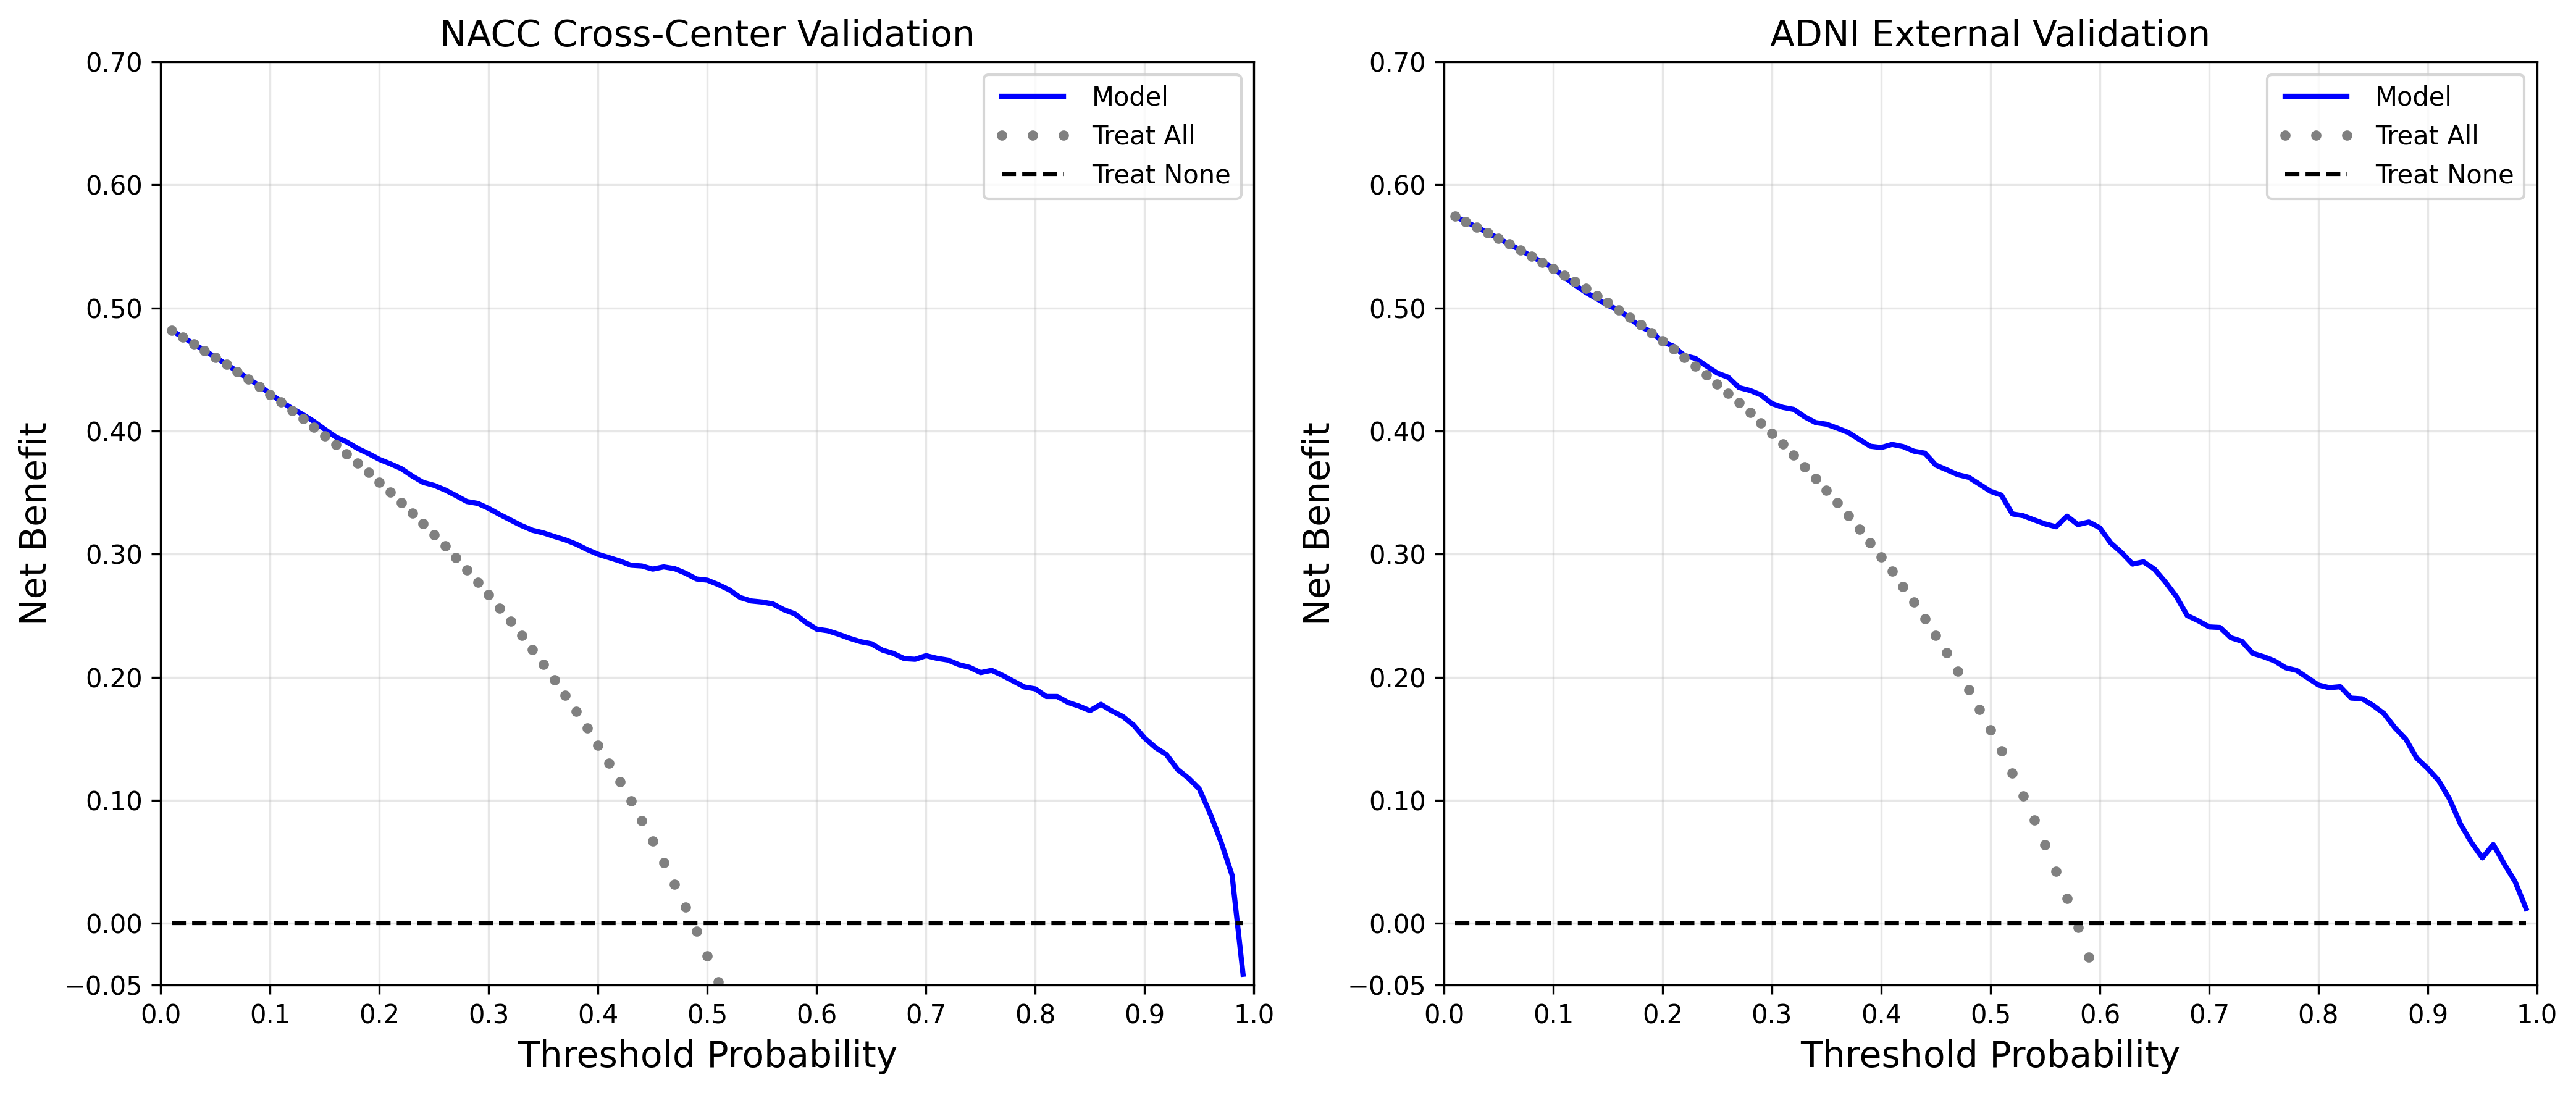
\includegraphics[width=1.0\textwidth]{figures/DCA/impaired_prediction_dca_both.png}
    \caption{The decision curve analysis (DCA) for the future NC vs. CI prediction task}
    \begin{minipage}{\textwidth}
      \footnotesize This figure illustrates the DCA curves of the NACC cross-center validation (left side) and the ADNI external validation (right side). "Treat All" refers to the assumption that all subjects are predicted to have CI in five years, and "Treat None" refers to the assumption that none of the subjects are predicted to have CI in five years.
    \end{minipage}
    \label{fig:future_nc_ci_dca}
\end{figure}

\subsubsection{External Validation Results for the Future CIND vs. Dementia Prediction Task}
The selected LR model for the future CIND vs. dementia prediction task was evaluated to determine its generalizability to unseen datasets. Table~\ref{tab:future_cind_dementia_results} provides a comparison of the model's performance in the internal cross-validation, NACC cross-center validation, and the ADNI external validation. The ROC curves for these validation stages are presented in Figure~\ref{fig:future_cind_dementia_roc}.

\begin{table}[!ht]
    \centering
    \caption{Performance of the selected logistic regression model in internal and external validation for the future CIND vs. dementia prediction task}
    \label{tab:future_cind_dementia_results}
    \newcolumntype{C}{>{\centering\arraybackslash}X}
        \begin{tabularx}{\textwidth}{|c|c|C|C|}
            \hline
            \textbf{Metric} & \textbf{Internal CV} & \textbf{NACC Cross-center Validation} & \textbf{ADNI External Validation} \\
            \hline
            AUC & \makecell{0.759 \\ {\small \hl{(0.751--0.768)}}} & \makecell{0.805 \\ {\small \hl{(0.784--0.828)}}} & \makecell{0.780 \\ {\small \hl{(0.740--0.819)}}} \\ \hline
            G-mean & 0.757 & 0.803 & 0.780 \\ \hline
            Sensitivity & 0.714 & 0.746 & 0.787 \\ \hline
            Specificity & 0.804 & 0.864 & 0.773 \\ \hline
            F1-score & 0.773 & 0.811 & 0.715 \\
            \hline
            \multicolumn{4}{p{400pt}}{\footnotesize \hl{AUC: area under the curve, F1-score: harmonic mean of precision and recall, G-mean: geometric mean score, Sensitivity: recall of the dementia class, Specificity: recall of the CIND class.}}
        \end{tabularx}
\end{table}

\begin{figure}[ht]
    \centering
    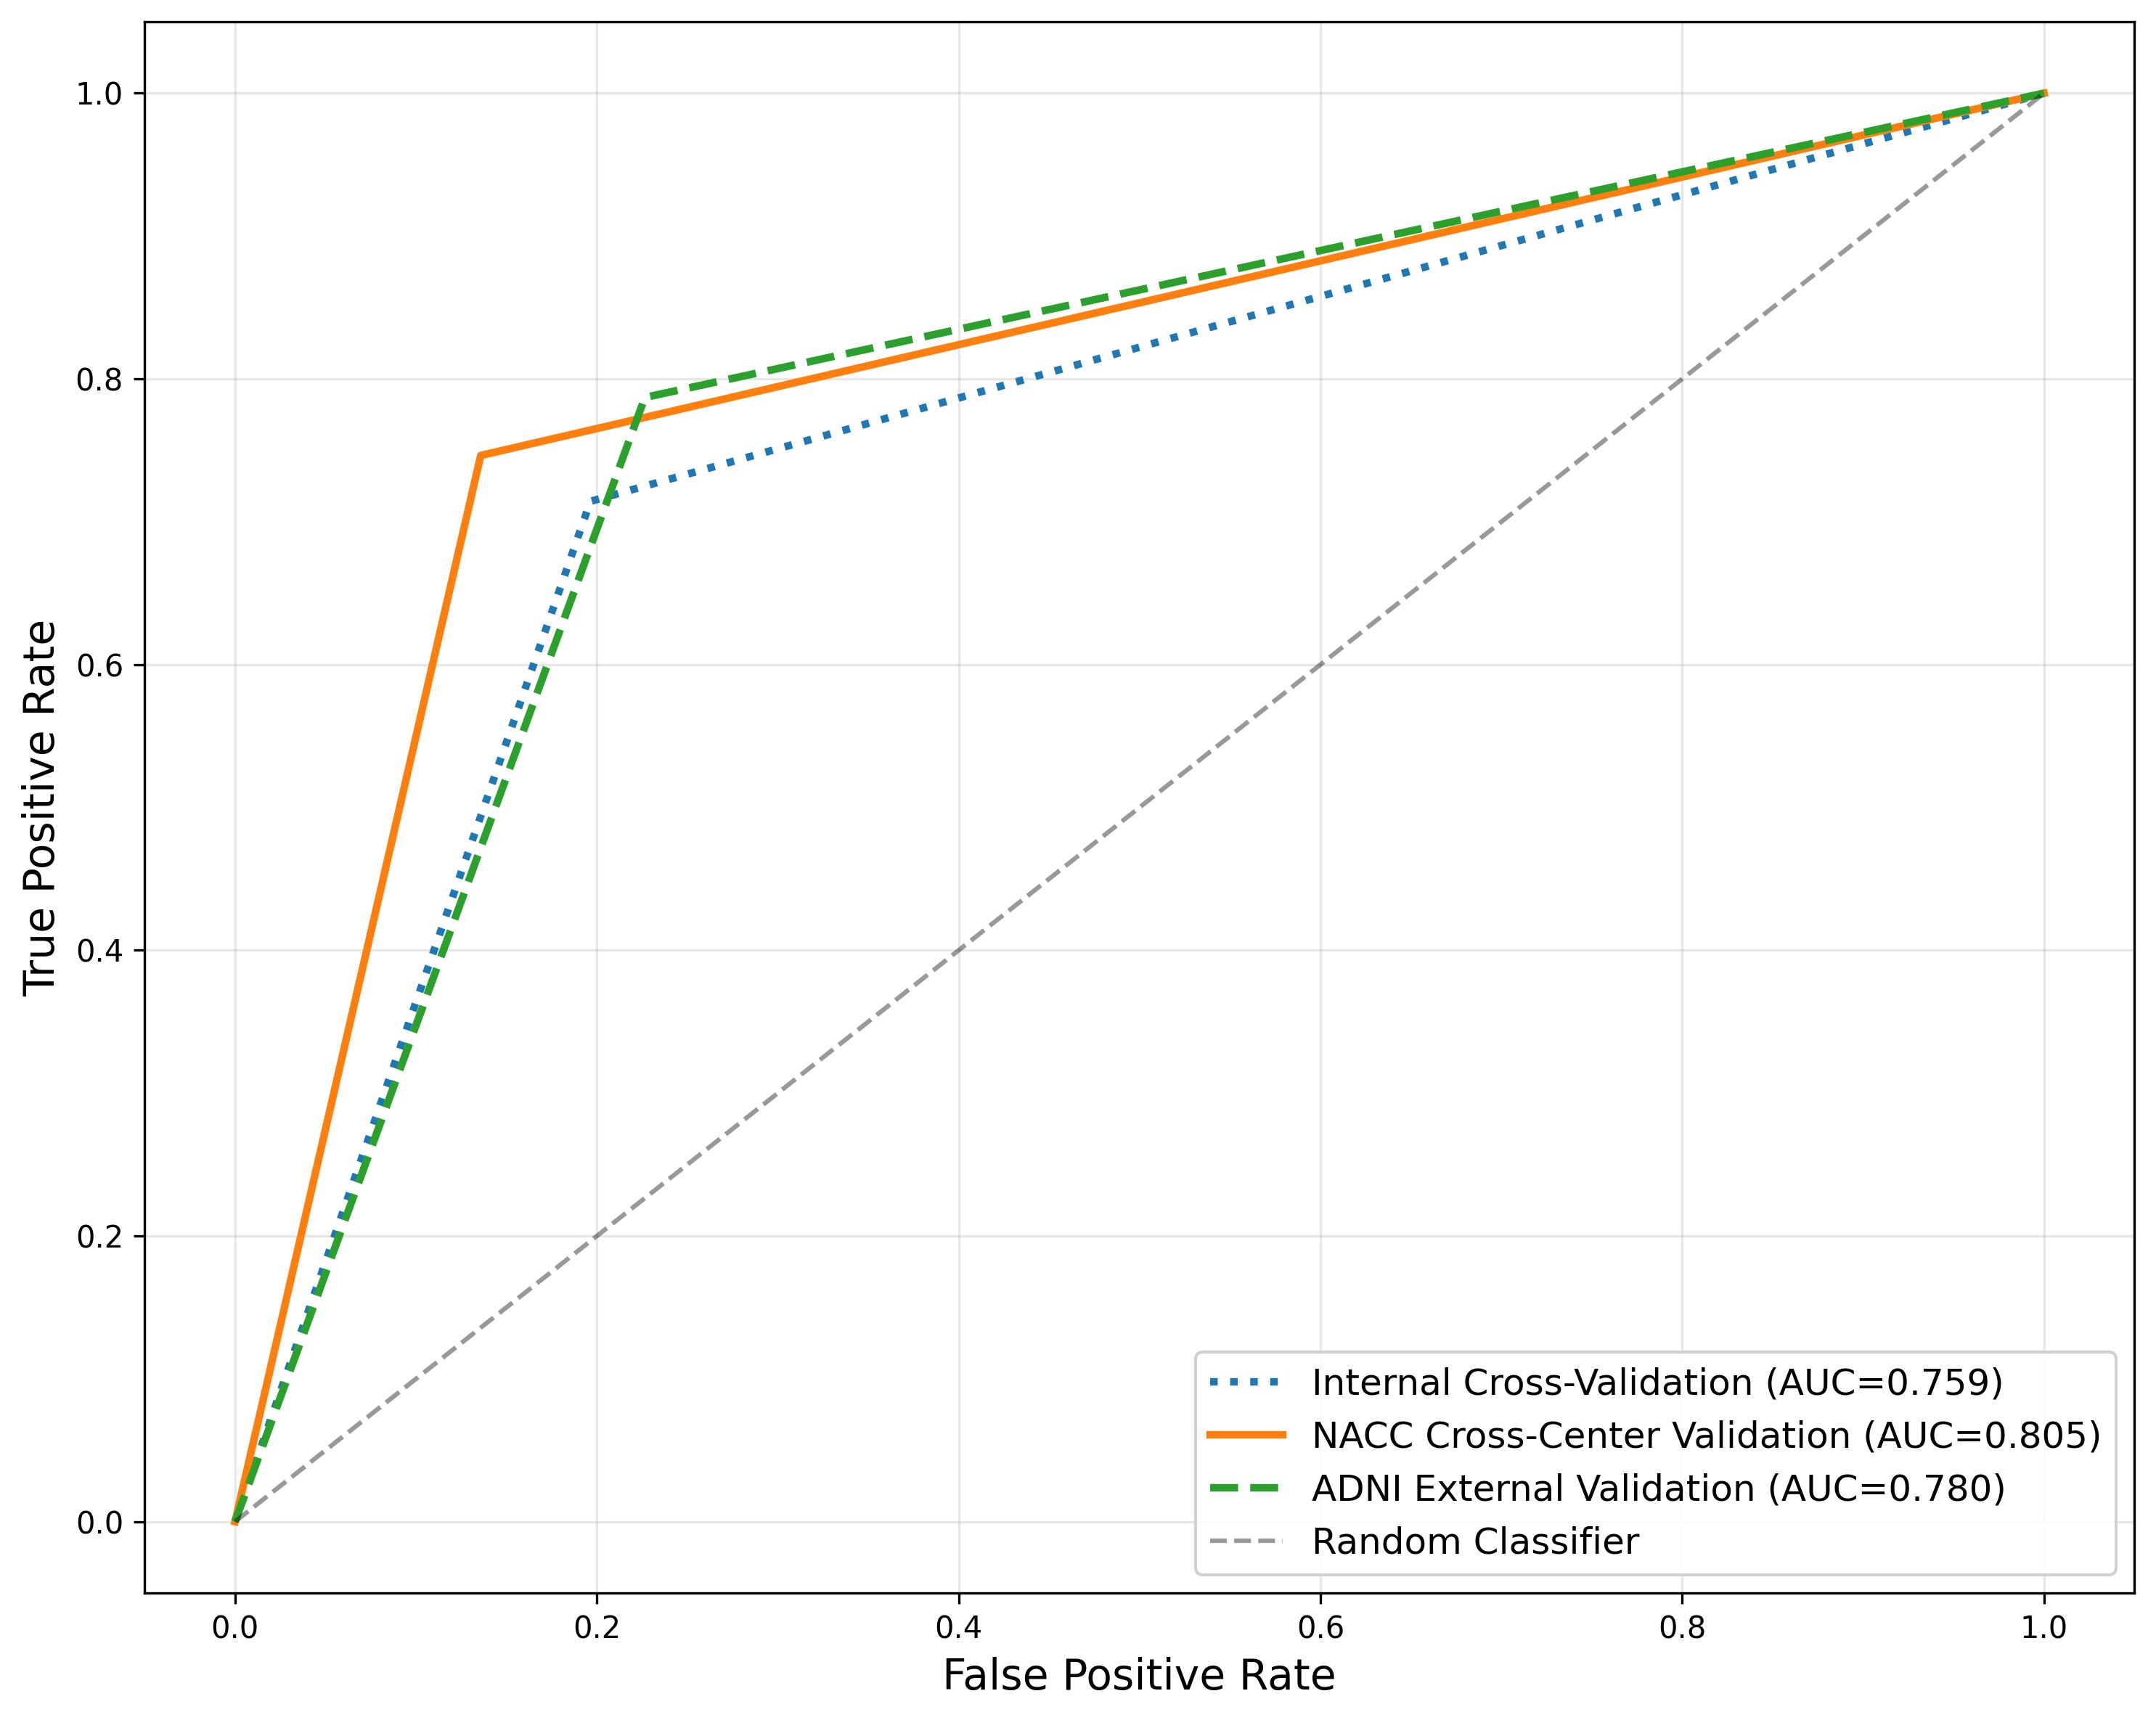
\includegraphics[width=0.7\textwidth]{figures/dementia_prediction_all_tests_roc_overlay.png}
    \caption{ROC curves comparing the performance of the logistic regression model for the future CIND vs. dementia prediction task}
    \begin{minipage}{\textwidth}
      \footnotesize \hl{The horizontal axis shows the false positive rate (1 -- specificity) and the vertical axis shows the true positive rate (sensitivity). Each curve represents one validation dataset.}
    \end{minipage}
    \label{fig:future_cind_dementia_roc}
\end{figure}

The LR model had a significant improvement in performance in the NACC cross-center validation compared to the internal CV. This result is similar to the previous prediction task. An improvement in sensitivity (0.714 to 0.746) and specificity (0.804 to 0.864) was observed. As a result, the AUC score increased from 0.759 to 0.805 and the G-mean increased from 0.757 to 0.803.  These results indicate that the model accurately generalized to the unseen data collected from different research.

The high generalizability of the LR model was also observed in the external validation on the ADNI dataset. The AUC score of 0.780 was higher than the internal CV baseline. This shows that the model can provide high classification performance even in a new clinical setting. A critical finding was noticed, which is the increase in sensitivity to 0.787. This is the highest sensitivity score across all three validation stages, indicating that the model is even more effective in correctly predicting future dementia risk in the ADNI cohort. 

In exchange for the increase in sensitivity, the LR model's specificity and F1-score dropped to 0.773 and 0.715, respectively. This drop in F1-score is largely driven by a significant reduction in precision (from 0.887 in the NACC cross-center validation to 0.655 in the ADNI external validation). This means that the model had a higher rate of false positives relative to true positives. Although a high number of false positives should be avoided, this result is in alignment with the clinical goal of a screening tool. In the context of predicting severe cognitive decline, it is safer for more patients to be flagged for further evaluation than missing actual cases of future dementia. Therefore, the model's ability to prioritize sensitivity on the external data supports its utility for early cognitive impairment prediction in real clinical practice. \hl{The improvement in AUC over the internal CV reached statistical significance in both validations (NACC cross-center p < 0.001, ADNI p = 0.016), which reflects the consistent gain observed in the external datasets.} The external validation results are reported with extended performance metrics in Table~\ref{table:lr-complete-perf-task4-apdx} in the appendix.

The selected LR model was calibrated to improve its estimation of future dementia risk. The calibration results for the external validation in the NACC and the ADNI datasets are shown in Figure~\ref{fig:future_cind_dementia_calib_curve}. In the NACC cross-center validation, the uncalibrated model assigned underestimated probabilities to subjects with moderate and low risk of dementia, while extreme probabilities were assigned to subjects with high risk. Using beta calibration, the spread of the probabilities was corrected (slope = 1.264), and the underestimation bias was reduced, especially in moderate risk thresholds (intercept = 0.111). As a result, the model calibration error (ECE) improved from 0.103 to 0.074, and the Brier score decreased from 0.149 to 0.139. Although the model's prediction improved, the model was still slightly miscalibrated as compared to the calibrated model in the future NC vs. CI prediction task.

\begin{figure}[ht]
    \centering
    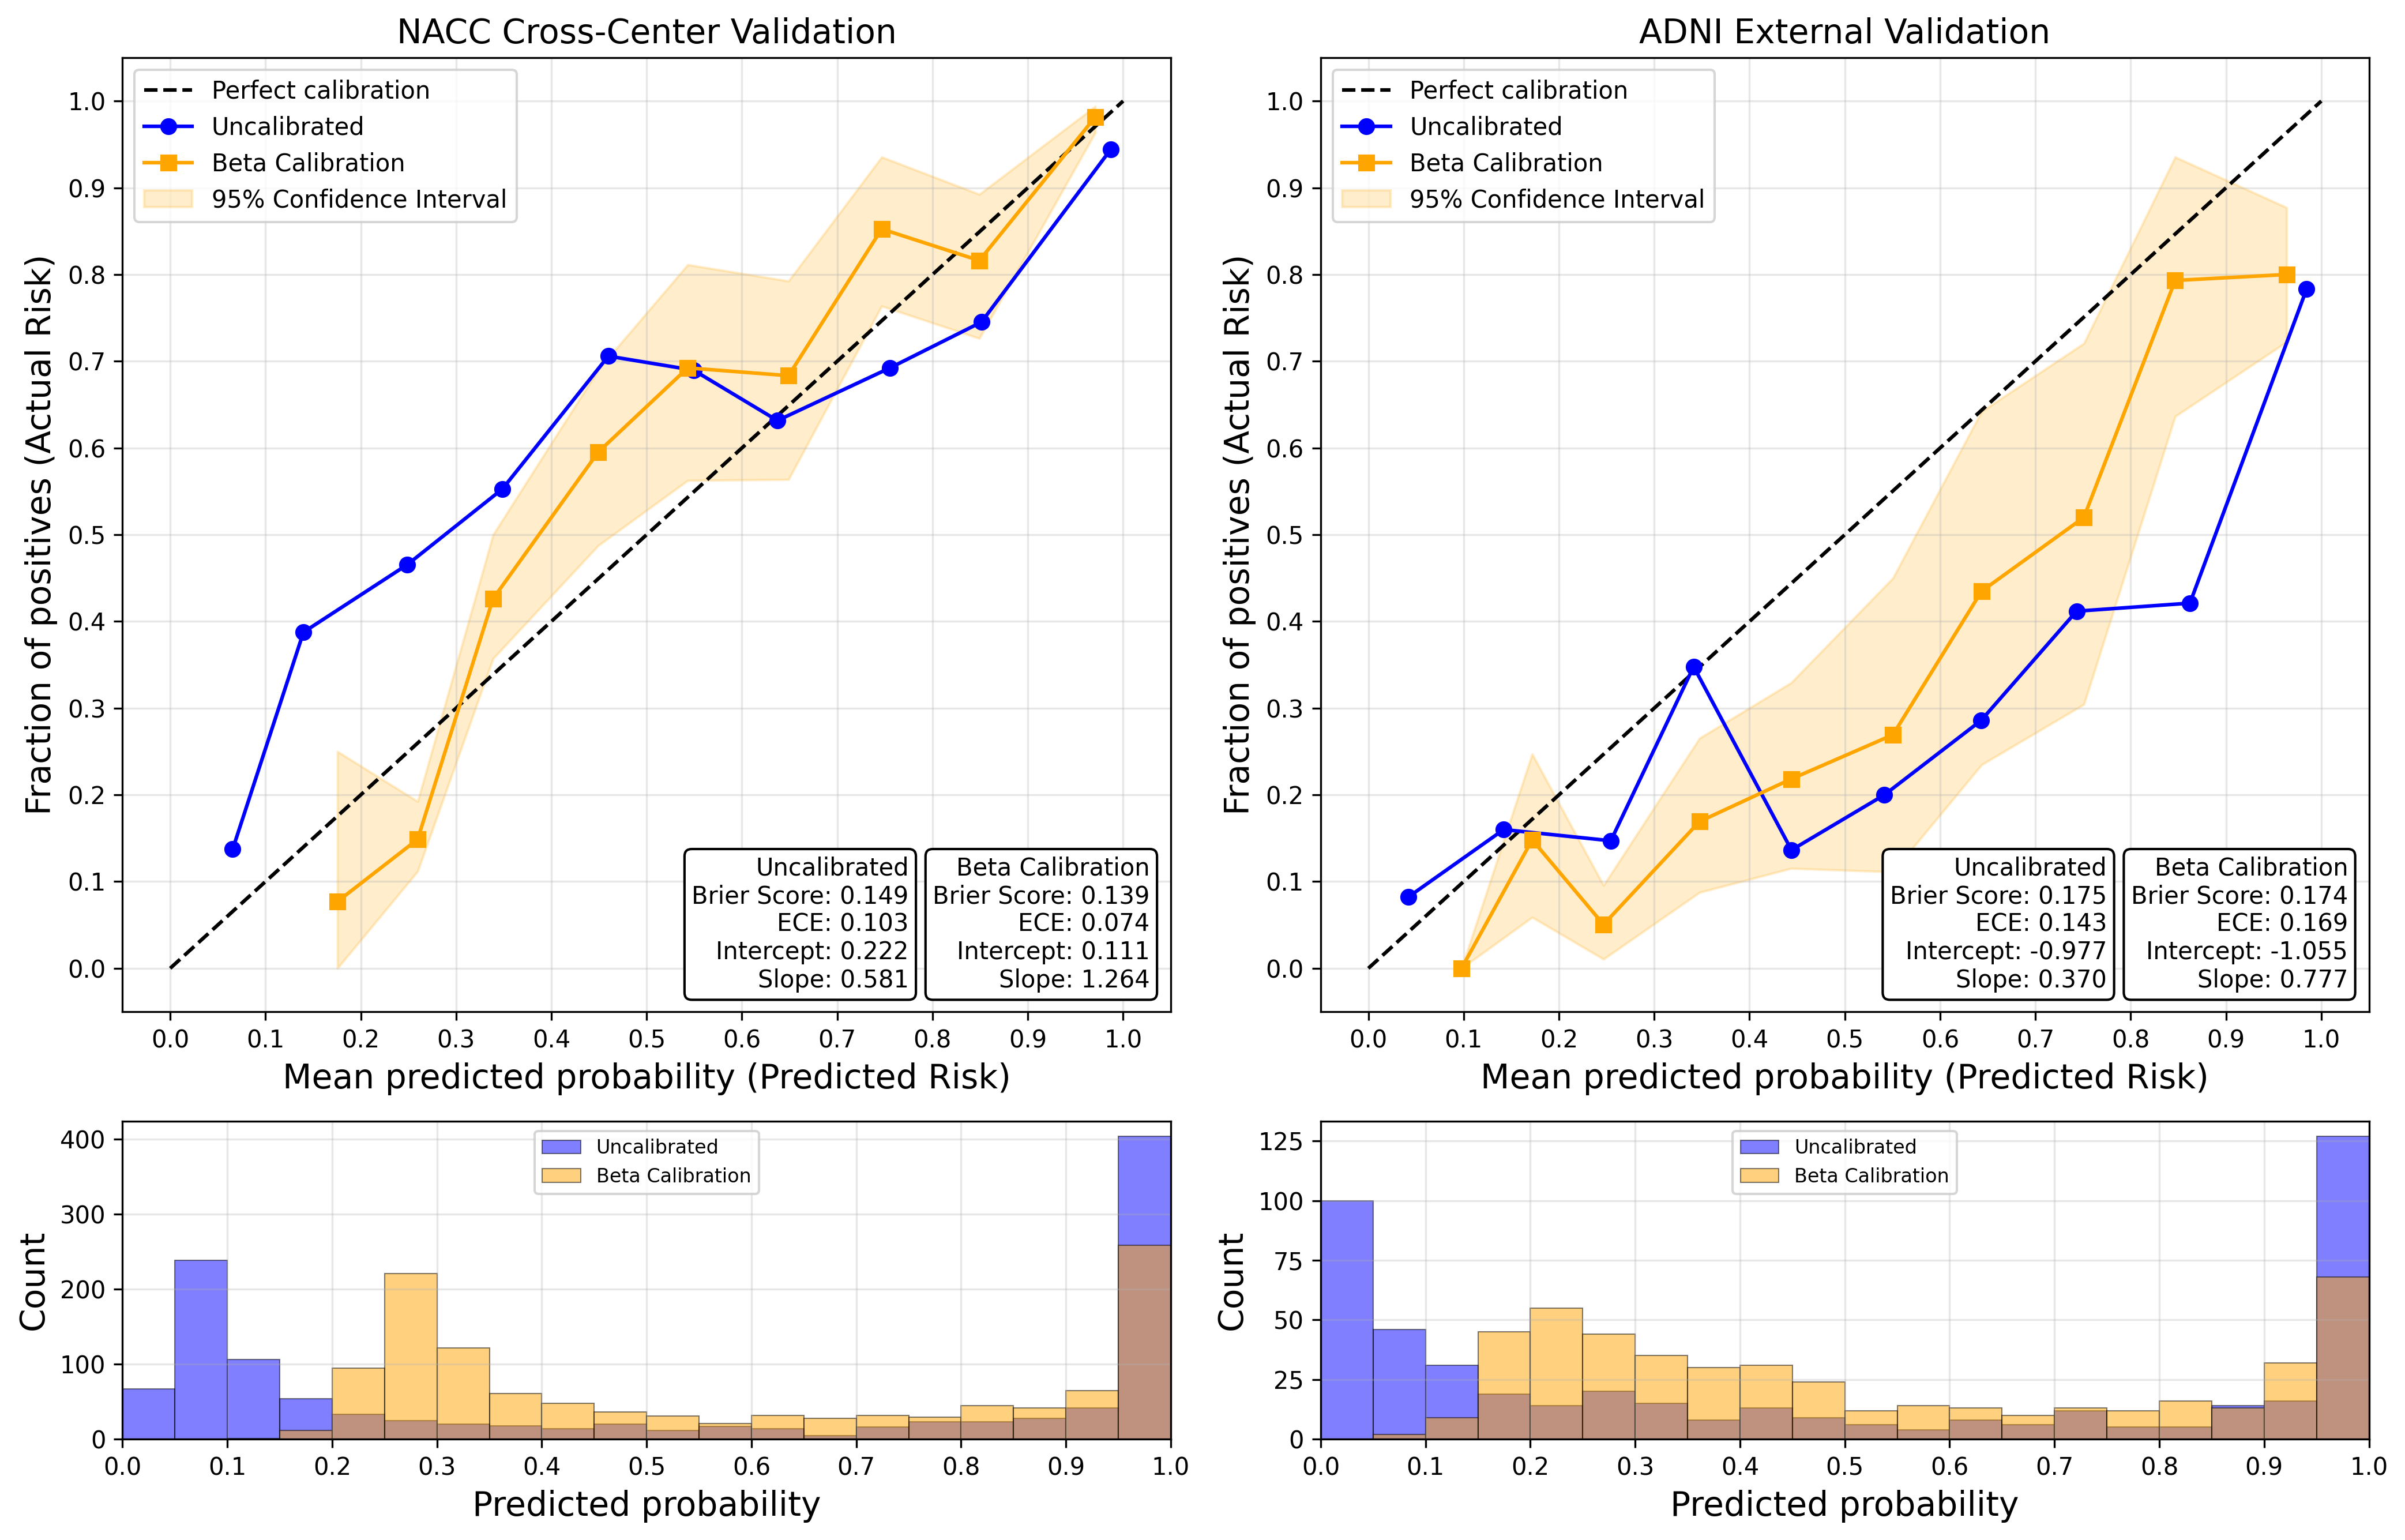
\includegraphics[width=1.0\textwidth]{figures/calibration/dementia_prediction_both_calibration_curve.png}
    \caption{Model calibration curves for the future CIND vs. dementia prediction task}
    \begin{minipage}{\textwidth}
      \footnotesize \hl{The horizontal axis shows the predicted probability and the vertical axis shows the observed frequency of the positive class. The diagonal line represents perfect calibration, and the curves compare the model before and after beta calibration.}
    \end{minipage}
    \label{fig:future_cind_dementia_calib_curve}
\end{figure}

The calibration results in the ADNI external validation were undesirable. In this dataset, the uncalibrated model severely overestimated the risk of dementia (intercept = -0.977). beta calibration could not fix the overestimation bias; instead, the ECE increased from 0.143 to 0.169. Applying the internal calibration parameters to the ADNI external data caused a mismatch between the predicted probabilities and the actual risk. The instability of the model predicted probabilities can be observed from the large confidence interval.

An evaluation of the clinical utility of the calibrated LR model was conducted using DCA as presented in Figure~\ref{fig:future_cind_dementia_dca}. The calibration of the model prediction improved the model's net benefit in the NACC cross-center validation, which outperformed the "treat all" and "treat none" strategies for the probability thresholds between 0.20 and 0.99. In contrast, the net benefit of the model was limited between the 0.18 and 0.79 thresholds in the ADNI external validation. Although the model demonstrated better clinical utility than the default strategies in the ADNI external, especially in low and intermediate thresholds, the DCA reflects the miscalibration of the model prediction observed in the calibration curve (intercept = -1.055).

\begin{figure}[ht]
    \centering
    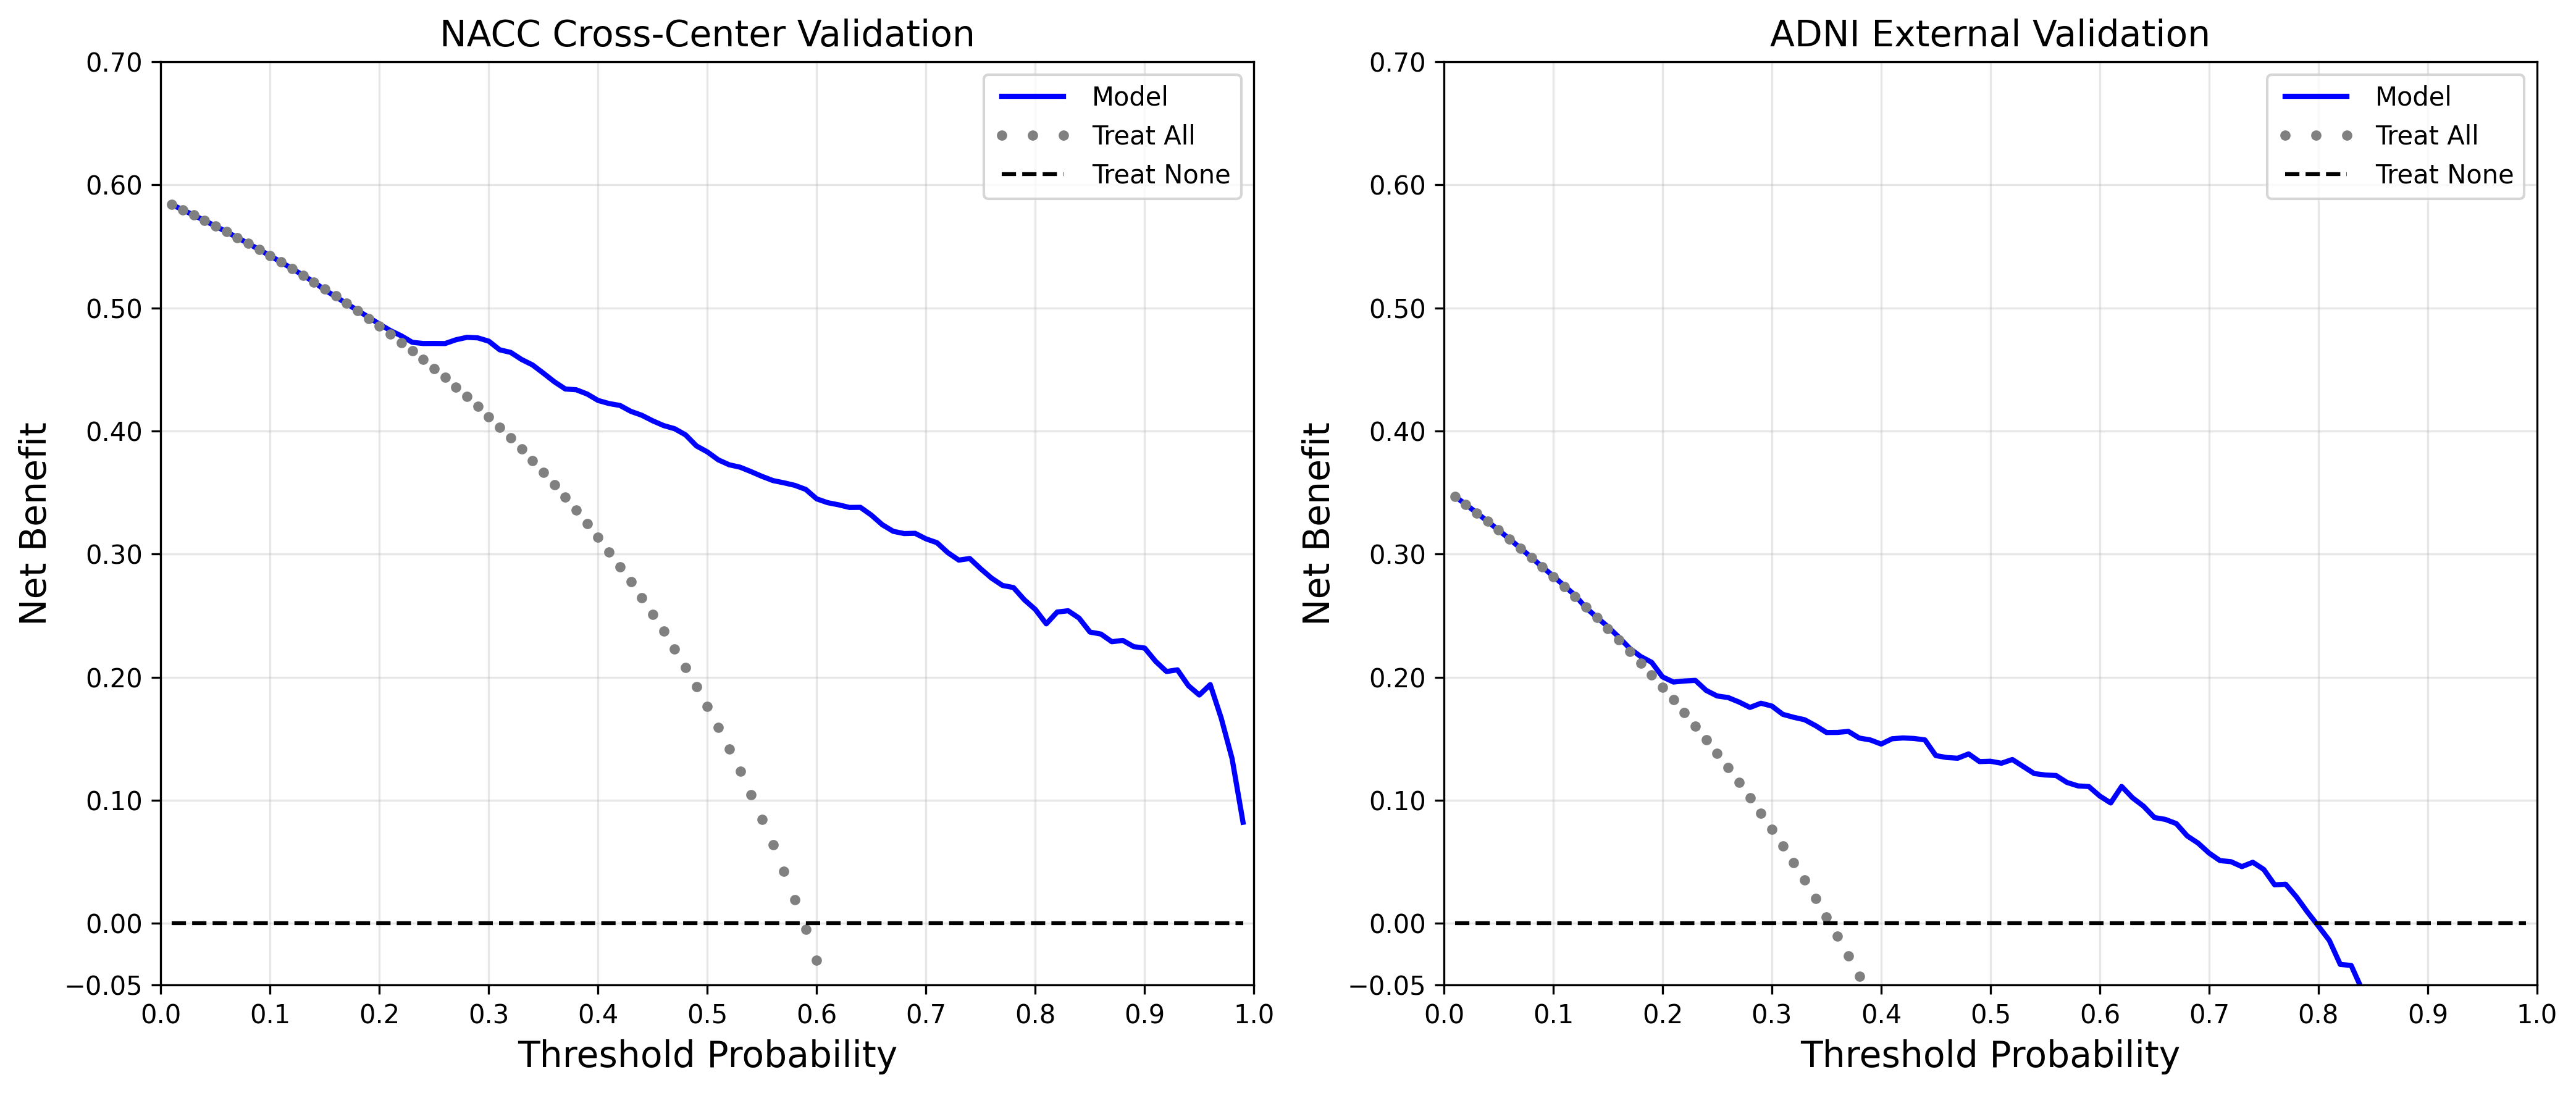
\includegraphics[width=1.0\textwidth]{figures/DCA/dementia_prediction_dca_both.png}
    \caption{The decision curve analysis (DCA) for the future CIND vs. dementia prediction task}
    \begin{minipage}{\textwidth}
      \footnotesize This figure illustrates the DCA curves of the NACC cross-center validation (left side) and the ADNI external validation (right side). "Treat All" refers to the assumption that all subjects are predicted to have dementia in five years, and "Treat None" refers to the assumption that all subjects are predicted to have CIND in five years.
    \end{minipage}
    \label{fig:future_cind_dementia_dca}
\end{figure}

The external validation results confirm that the developed models for predicting future cognitive status are generalizable. Both prediction models achieved high performance in the ADNI study, especially in detecting cases with high risk (sensitivity). The models also scored high accuracy in the NACC cross-center validation compared to the internal CV. In addition, the models presented excellent calibration and clinical utility to accurately estimate the risk of CI and dementia, especially in the NACC cross-center validation. These results validate the second objective of the study, demonstrating that accessible baseline data can be used to effectively predict the risk of cognitive impairment up to five years in the future across diverse clinical settings.

\subsection{Model Explainability Results}

\subsubsection{Model Explainability Results for the Future NC vs. CI Prediction Task}
The features in the future prediction of NC vs. CI are ranked according to their global importance in Figure~\ref{figure:nc_ci_prediction_feature_importance}. A similar feature importance ranking can be observed in both the NACC cross-center validation and the ADNI external validation. This is confirmed by the Spearman’s rank correlation coefficient of 0.83 ($p$ < 0.05). In both tests, the model relied heavily on a combination of functional activities, self-reported memory issues (MEMPROB), and behavioral factors (IRR). The feature representing self-reported memory issues was identified as the most important predictor. The only notable difference in the feature importance of the two external validation was the SHAP value of the IRR feature. It was observed that the IRR feature has a significantly higher influence on the model prediction in the ADNI external validation compared to the NACC cross-center validation.

\begin{figure}[ht]
    \centering
    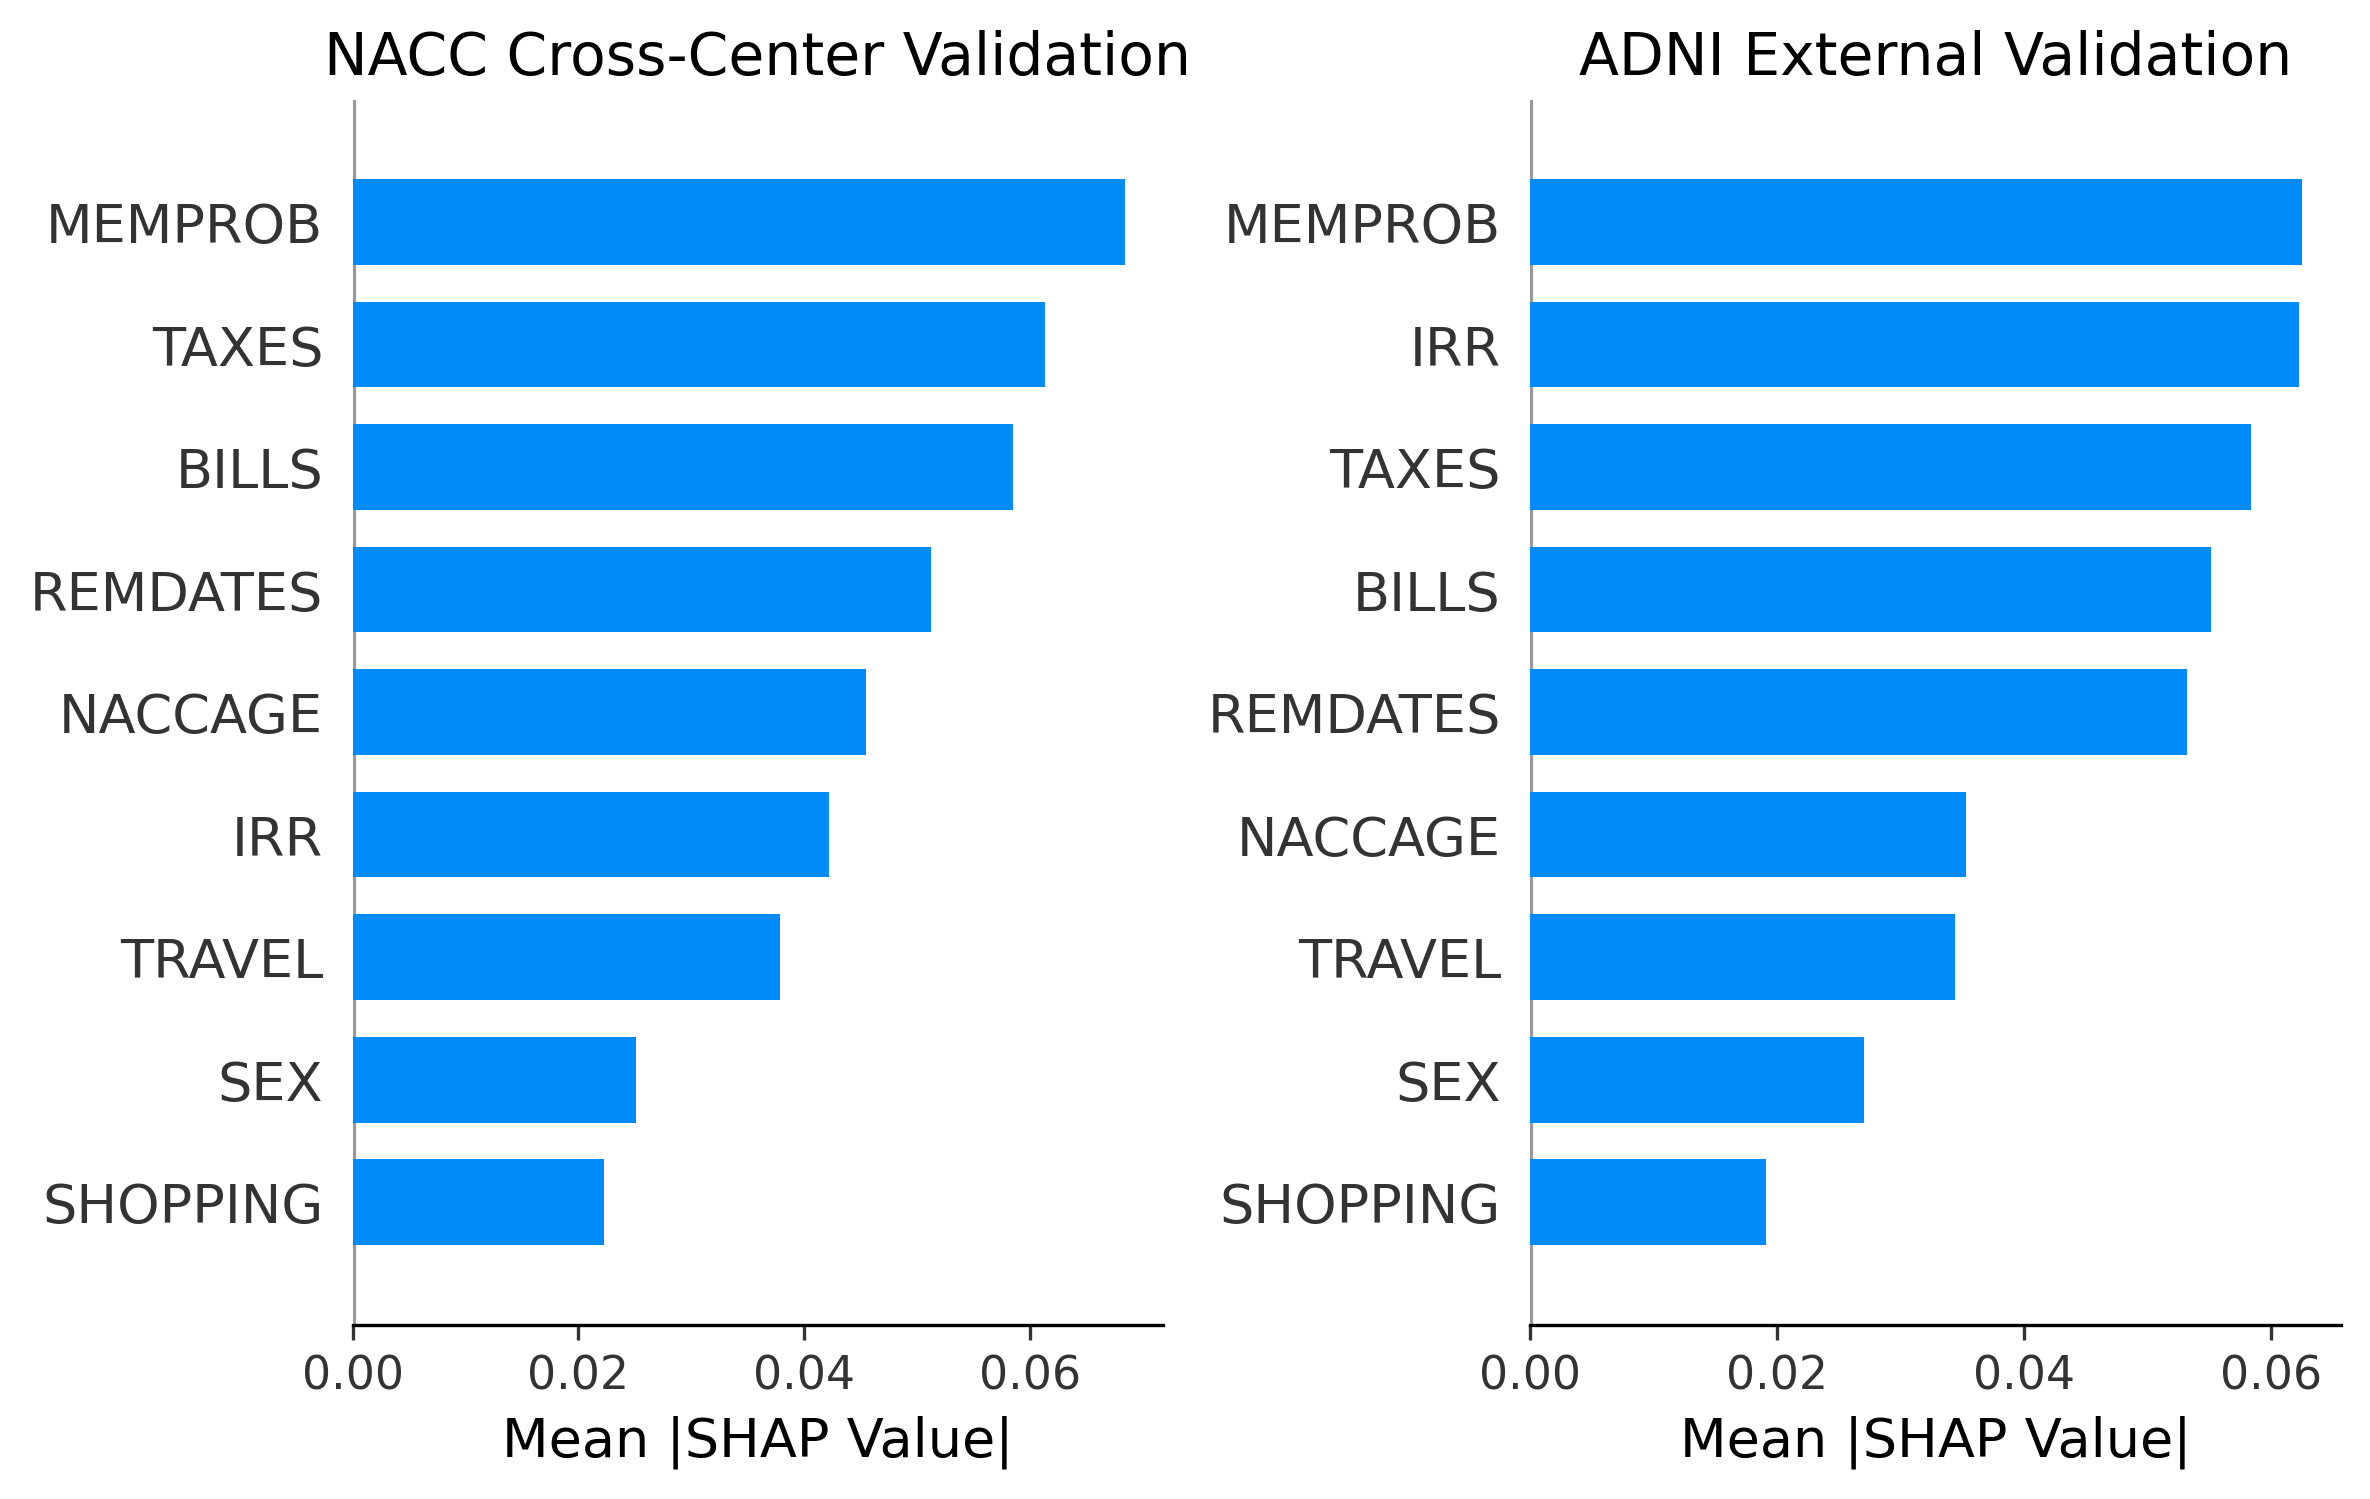
\includegraphics[width=1.0\textwidth]{figures/XAI/impaired_prediction_both_feature_importance_comparison.png}
    \caption{Feature importance in the NACC cross-center validation and the ADNI external validation for the future NC vs. CI prediction task}
    \begin{minipage}{\textwidth}
      \footnotesize \hl{The bars represent the mean absolute SHAP value of each feature, which ranks the contribution of the feature to the model prediction in the two validation datasets.}
    \end{minipage}
    \label{figure:nc_ci_prediction_feature_importance}
\end{figure}

Analyzing the local explanation of the selected model is crucial, as subjects with different risk profiles might have similar prediction outcomes. Figure~\ref{figure:nc_ci_prediction_pos_waterfall} demonstrates two correctly predicted CI instances with the same probabilities of 55\%. The demographic characteristics (male gender and older age of 79 years), together with a history of never performing tax-related tasks (TAXES), were the main risk factors of CI for Instance A. In contrast, \textit{Instance B} has a different risk profile mainly associated with difficulty remembering dates and appointments (REMDATES).

\begin{figure}[ht]
    \centering
    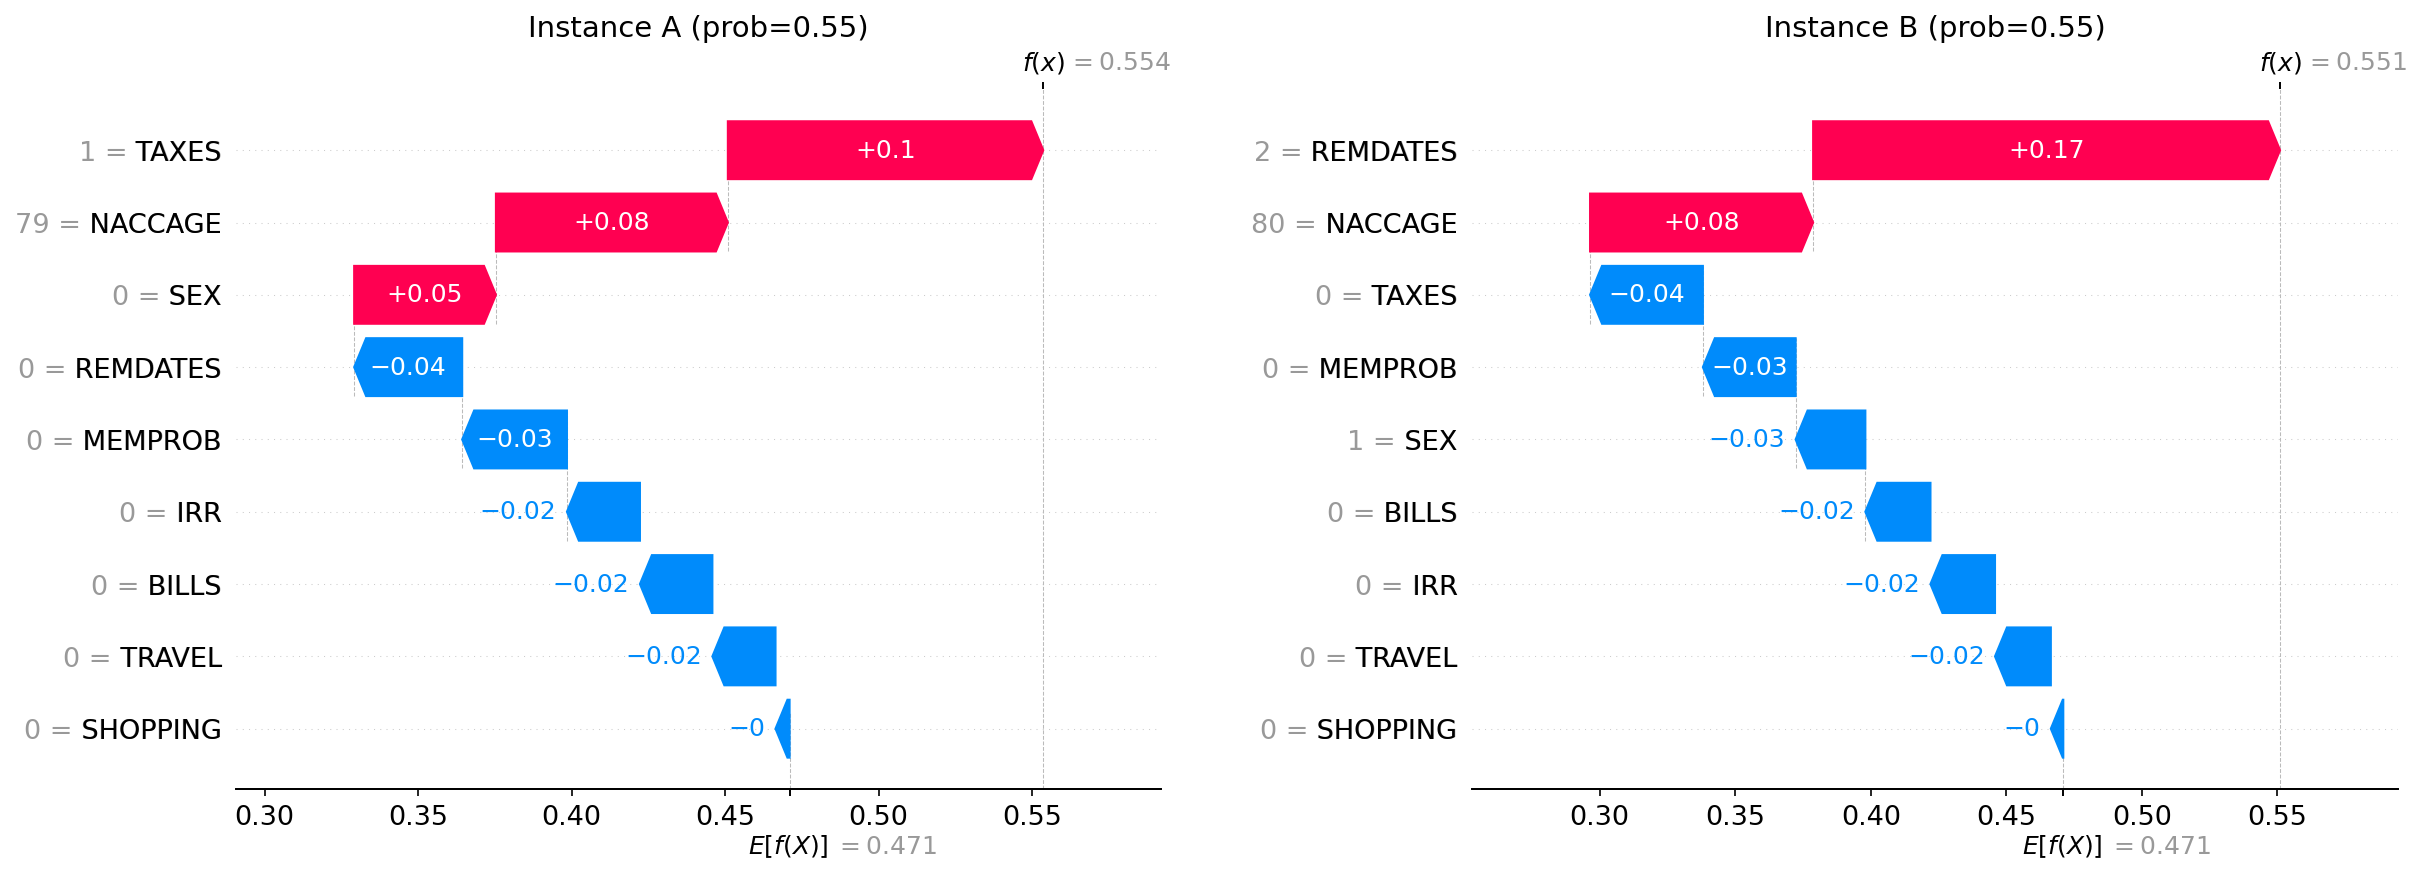
\includegraphics[width=1.0\textwidth]{figures/XAI/impaired_prediction_adni_true_positive_waterfall.png}
    \caption{SHAP waterfall plots for two instances correctly predicted as having risk of cognitive impairment within five years in future}
    \begin{minipage}{\textwidth}
      \footnotesize \hl{The plot shows how the value of each feature shifts the prediction from the base value to the final predicted probability for a single instance.}
    \end{minipage}
    \label{figure:nc_ci_prediction_pos_waterfall}
\end{figure}

A similar analysis was also performed on two instances correctly predicted as NC. Figure~\ref{figure:nc_ci_prediction_neg_waterfall} displays the waterfall plots of both instances. \textit{Instance A} has a normal ability to perform all functional activities, which reduced the probability of developing CI despite the high demographic risk of being an 84-year-old male. The younger female subject represented by \textit{Instance B} has a similar protective functional profile, except she has never done a tax filing before. It is interesting that this instance is similar to \textit{Instance A} in Figure~\ref{figure:nc_ci_prediction_pos_waterfall}, correctly predicted as cognitively impaired, with sex being the only major difference. This contrast highlights how interaction between features can change the predictive risk of cognitive impairment.

\begin{figure}[ht]
    \centering
    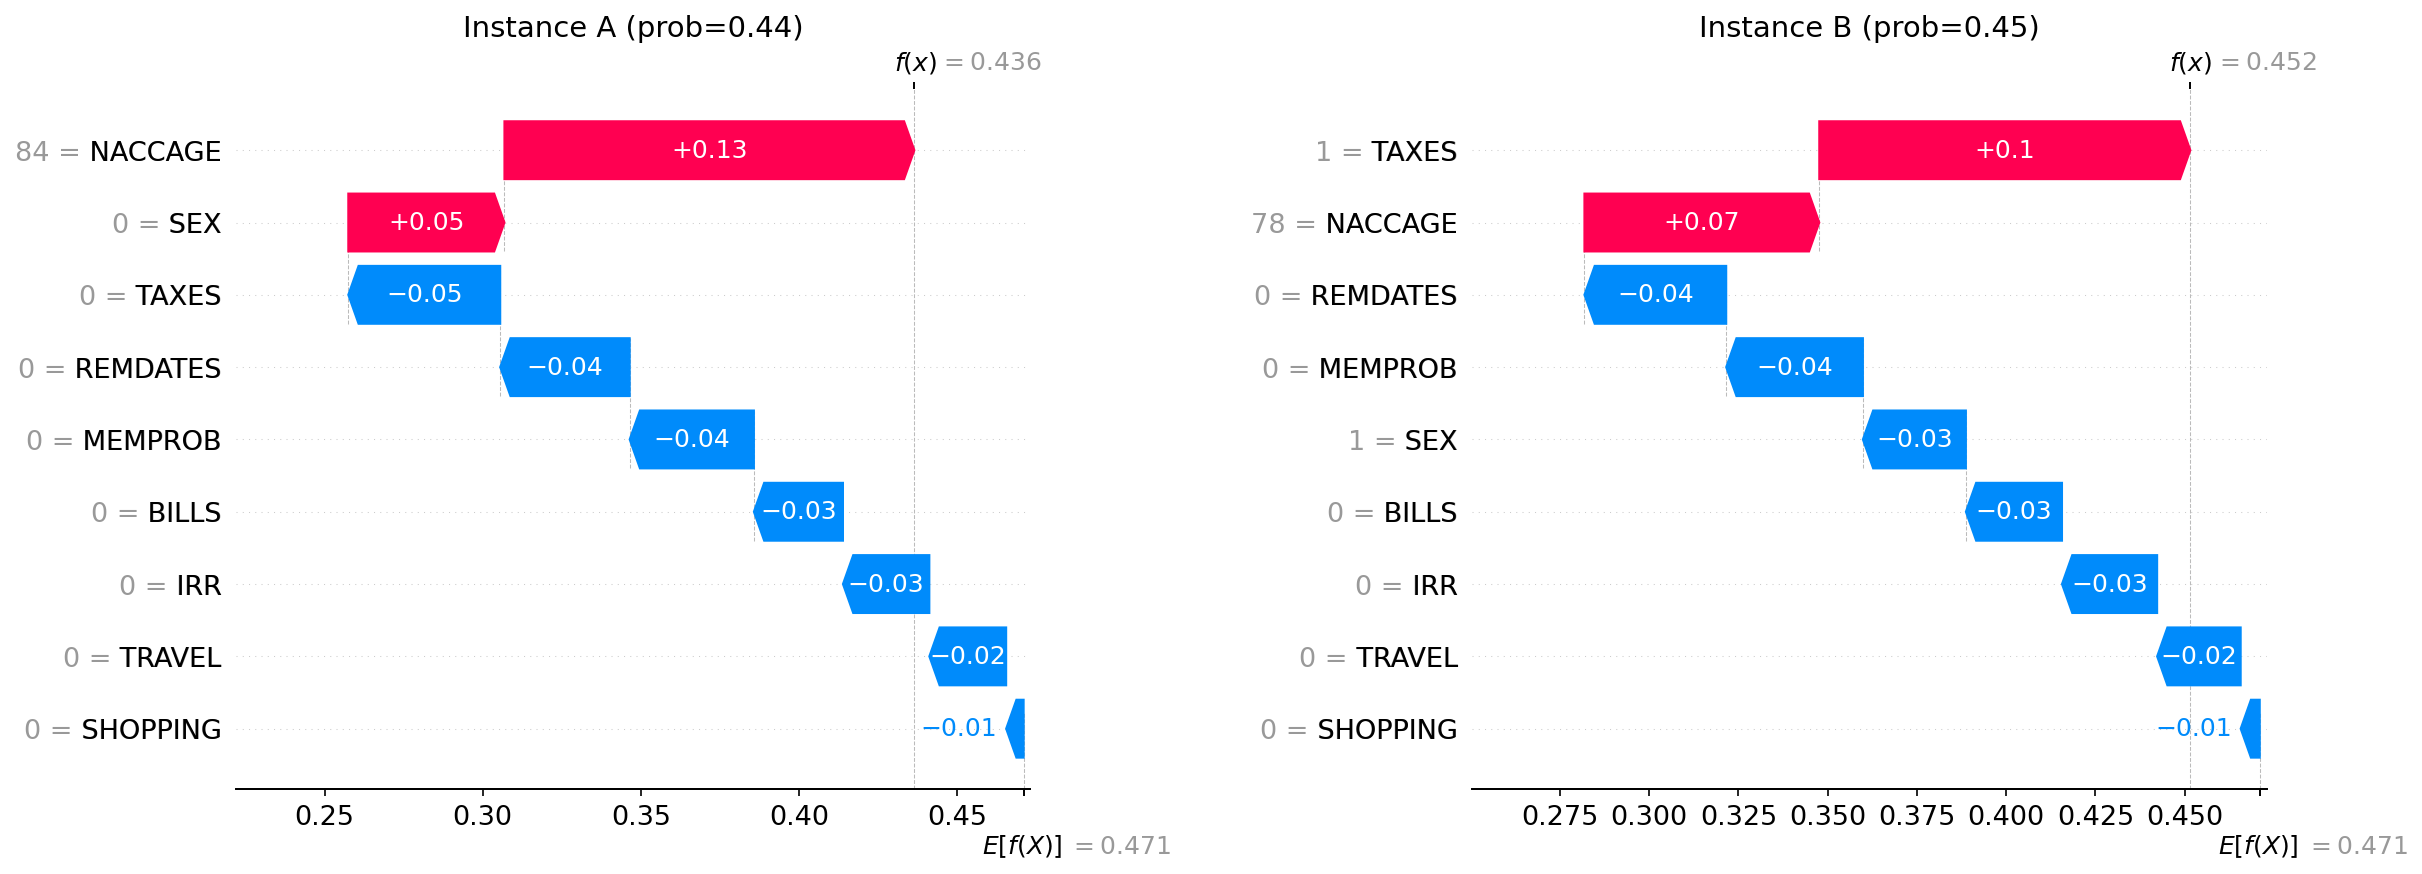
\includegraphics[width=1.0\textwidth]{figures/XAI/impaired_prediction_adni_true_negative_waterfall.png}
    \caption{SHAP waterfall plots for two instances correctly predicted as normal cognition within five years in future}
    \begin{minipage}{\textwidth}
      \footnotesize \hl{The plot shows how the value of each feature shifts the prediction from the base value to the final predicted probability for a single instance.}
    \end{minipage}
    \label{figure:nc_ci_prediction_neg_waterfall}
\end{figure}

The results of using DiCE to generate counterfactual examples are presented in Figure~\ref{figure:nc_ci_prediction_dice_stat}. DiCE had an excellent success rate in providing suggestions to prevent the potential CI risk early, with valid counterfactual examples generated for all ADNI external data instances. However, the range of risk prevention suggestions (counterfactual examples) available to each individual was more limited compared to the classification tasks presented in section \ref{sec:cls-xai}. On average, the majority of ADNI instances (69\%) receive only one valid suggestion to reverse their predicted prognosis from CI to NC.

\begin{figure}[ht]
    \centering
    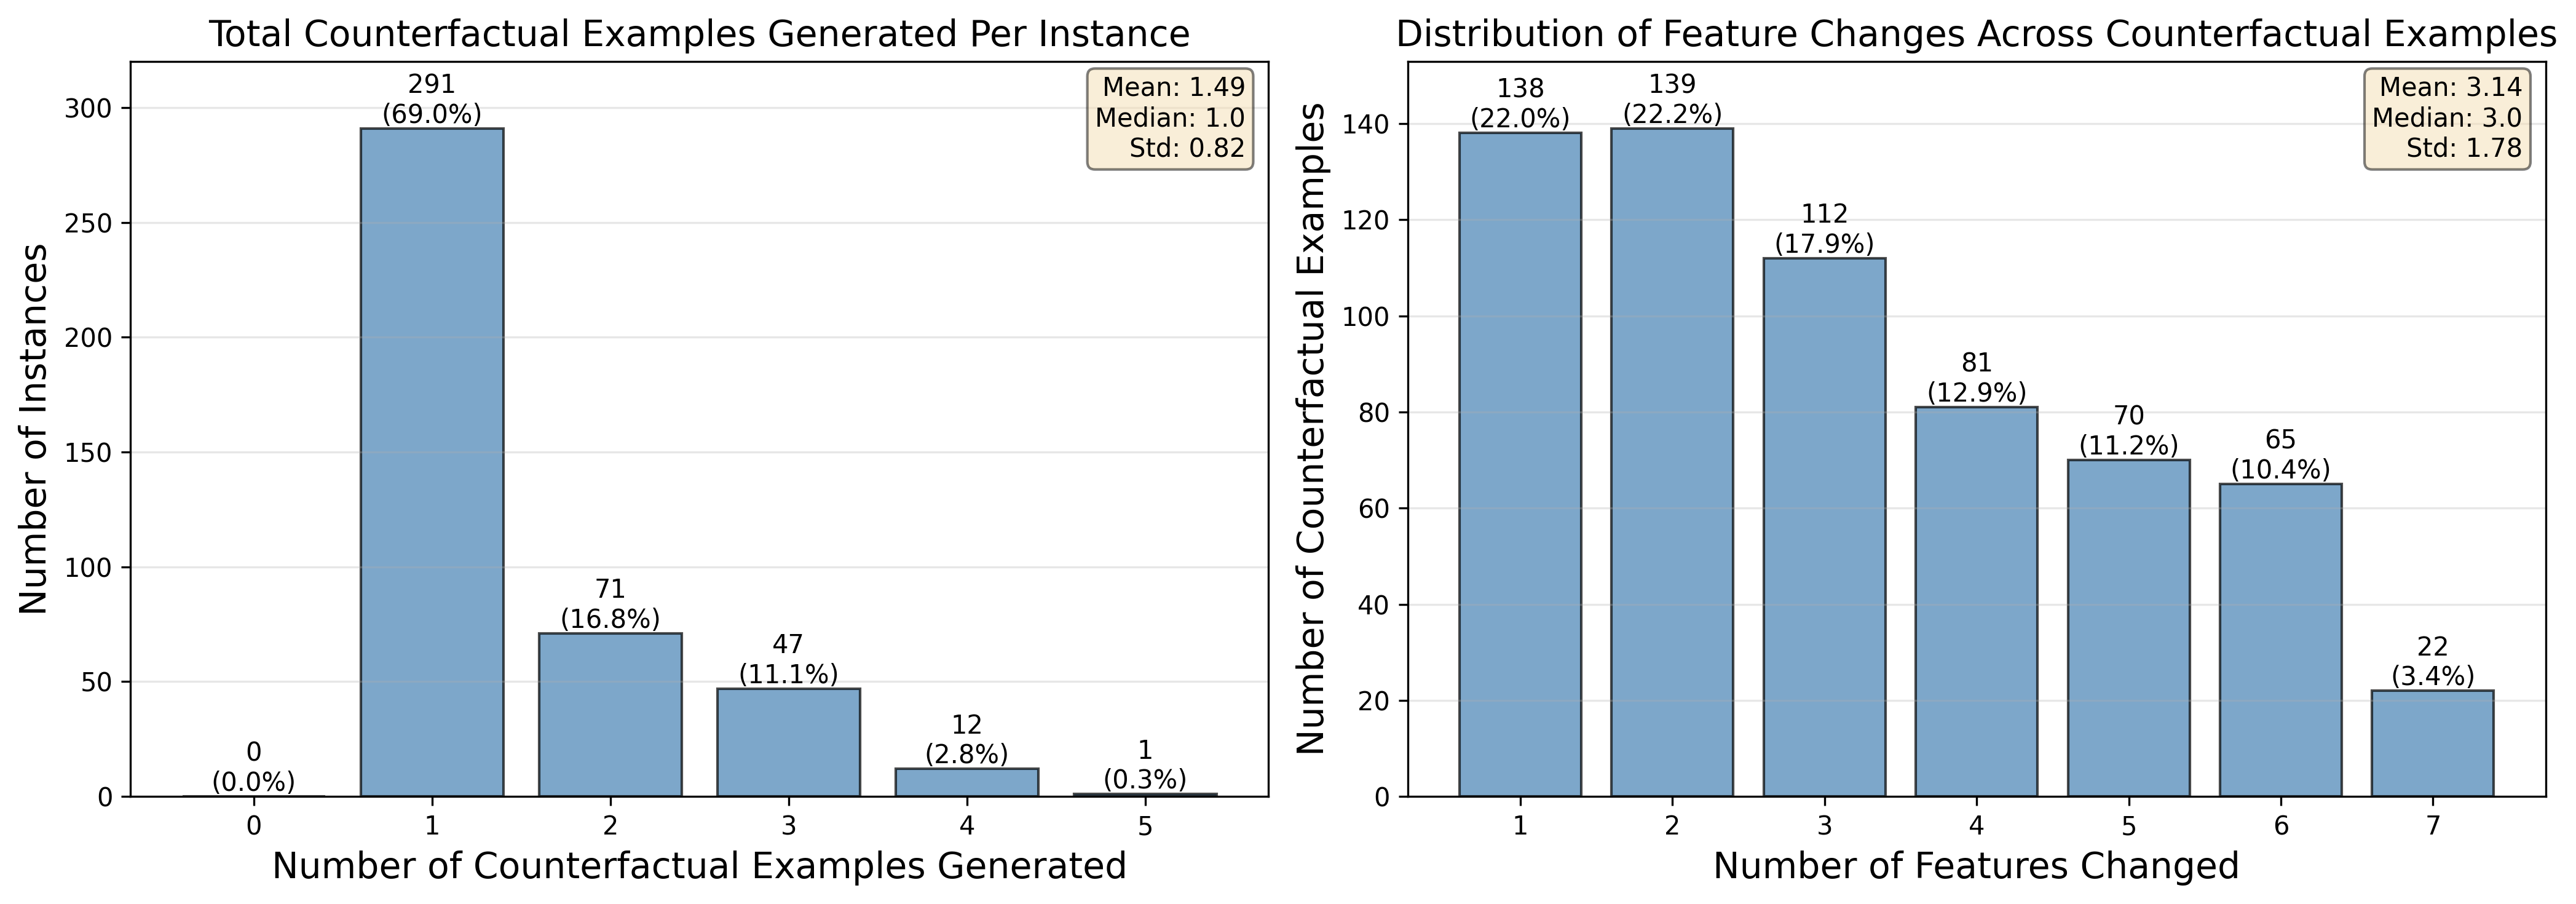
\includegraphics[width=1.0\textwidth]{figures/XAI/impaired_prediction_adni_kdtree_dice_stats.png}
    \caption{Summary of generated counterfactual examples for changing predicted risk from cognitive impairment to normal cognition}
    \label{figure:nc_ci_prediction_dice_stat}
\end{figure}

Regarding the feasibility of these interventions, the distribution of feature changes in Figure~\ref{figure:nc_ci_prediction_dice_stat} suggests that the risk of CI can be prevented early with minimal changes in risk factors. This is possible by modifying up to 3 of the 7 alterable features. According to the presented results, a significant proportion of the generated counterfactuals (44.2\%) required the change of only one or two features. This indicates that risk prevention plans that focus on a few risk factors could be enough to improve future cognitive status. The counterfactual explanation in the NACC cross-center validation had similar results with slightly higher feature changes required to generate the counterfactual examples. The results are presented in Figure~\ref{figure:dice-nacc-task3-apdx} in the appendix.

The most critical features that drive these interventions are ranked in Figure~\ref{figure:nc_ci_prediction_dice_feature_importance}. Remembering dates and appointments (REMDATES) was the most frequently modified feature (58\%), followed closely by handling taxes (TAXES, 55\%) and paying bills (BILLS, 52\%). Behavioral conditions were also found to be one of the key intervention factors in the ADNI external validation, with irritability (IRR) being modified in 51\% of the cases. Table~\ref{table:cfe-adni-task3-apdx} in the appendix presents counterfactual examples that illustrate how the feature values of a random subject with a future predicted risk of CI can be changed to prevent the risk.

\begin{figure}[ht]
    \centering
    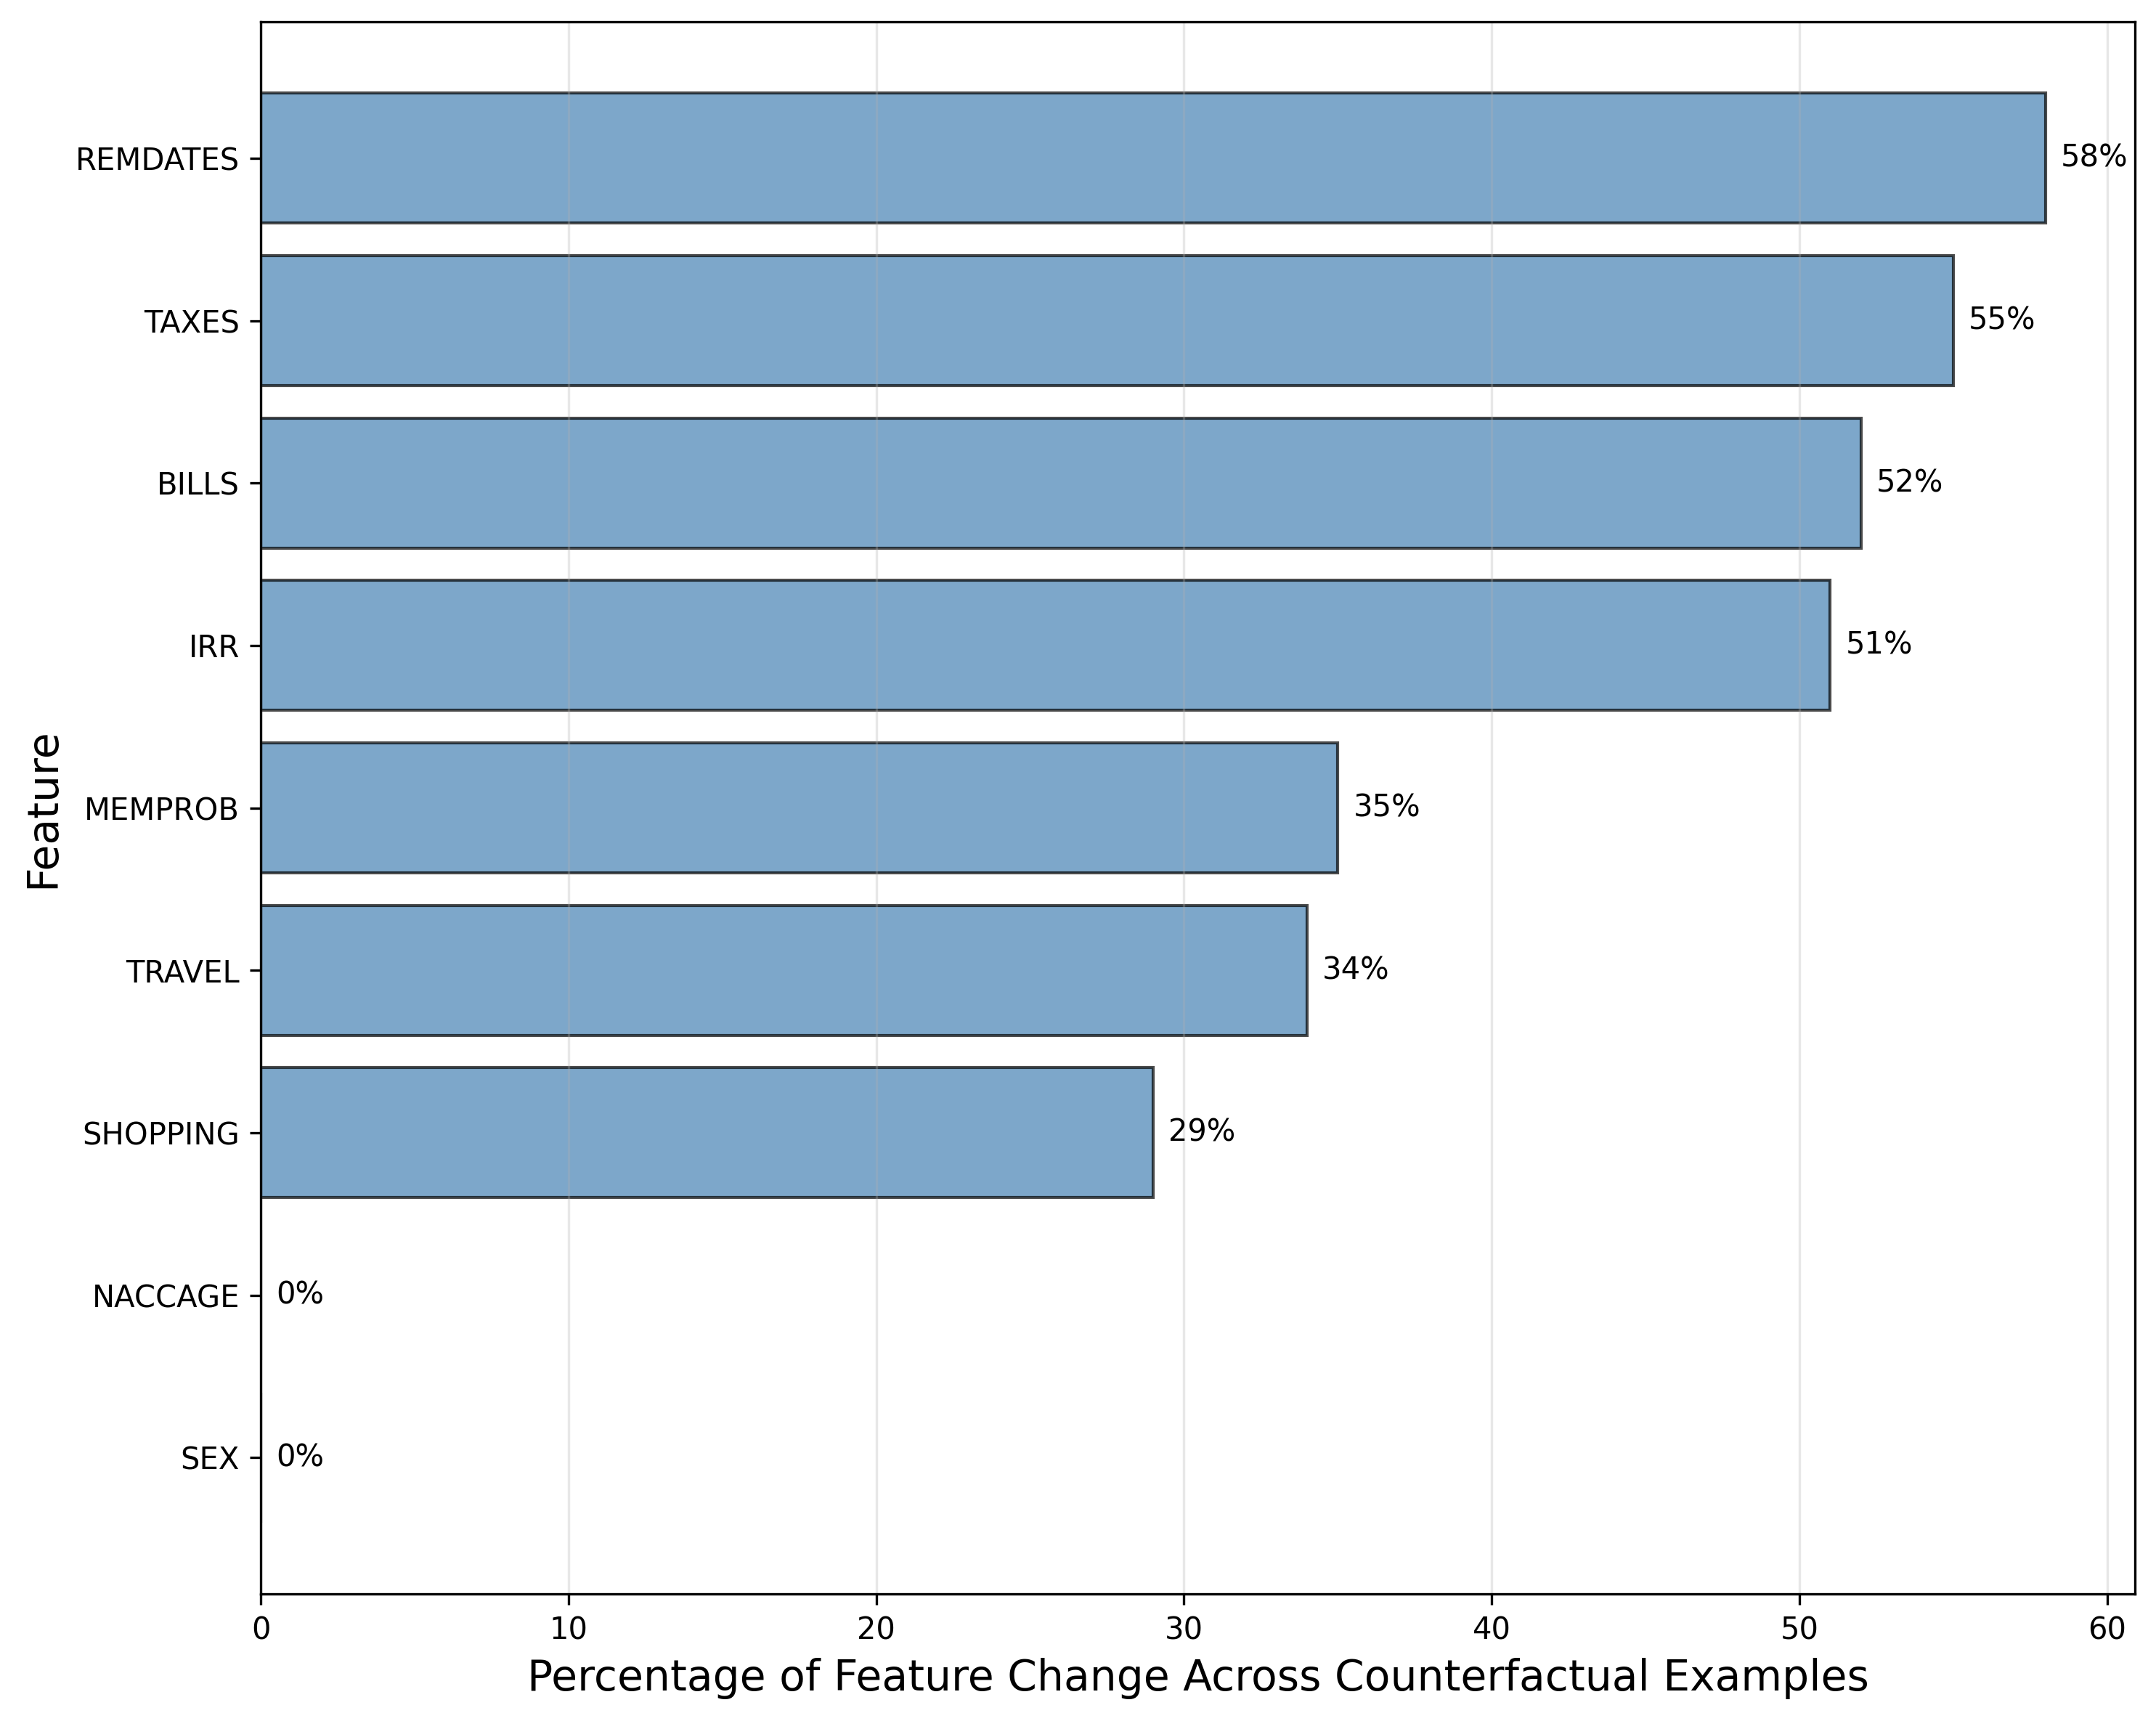
\includegraphics[width=1.0\textwidth]{figures/XAI/impaired_prediction_adni_kdtree_dice_global_importance.png}
    \caption{Feature importance ranking based on counterfactual explanations for the future NC vs. CI prediction task}
    \begin{minipage}{\textwidth}
      \footnotesize The features are ranked based on the percentage of times they were modified to generate valid counterfactual examples. The rank highlights the most critical features for risk intervention. Demographic features (NACCAGE and SEX) show 0\% importance because they were set as invariable features in the counterfactual generation process.
    \end{minipage}
    \label{figure:nc_ci_prediction_dice_feature_importance}
\end{figure}

\subsubsection{Model Explainability Results for the Future CIND vs. Dementia Prediction Task}
The global feature importance ranking of this prediction task is demonstrated in Figure~\ref{figure:cind_dementia_prediction_feature_importance}. The ranking of features is significantly similar in both the NACC cross-center validation and the ADNI external validation. This similarity is measured by Spearman’s rank correlation coefficient of 0.98 ($p$ < 0.05). In both cohorts, the model’s prediction was strongly influenced by measures of functional activities, specifically the ability to manage financial matters (BILLS and TAXES). The difficulty in remembering dates (REMDATES) and traveling (TRAVEL) also have high SHAP values. These results were observed in other classification and prediction tasks. In contrast, body mass index (NACCBMI) and symptoms such as energy levels (ENERGY) showed considerably lower importance scores.

\begin{figure}[ht]
    \centering
    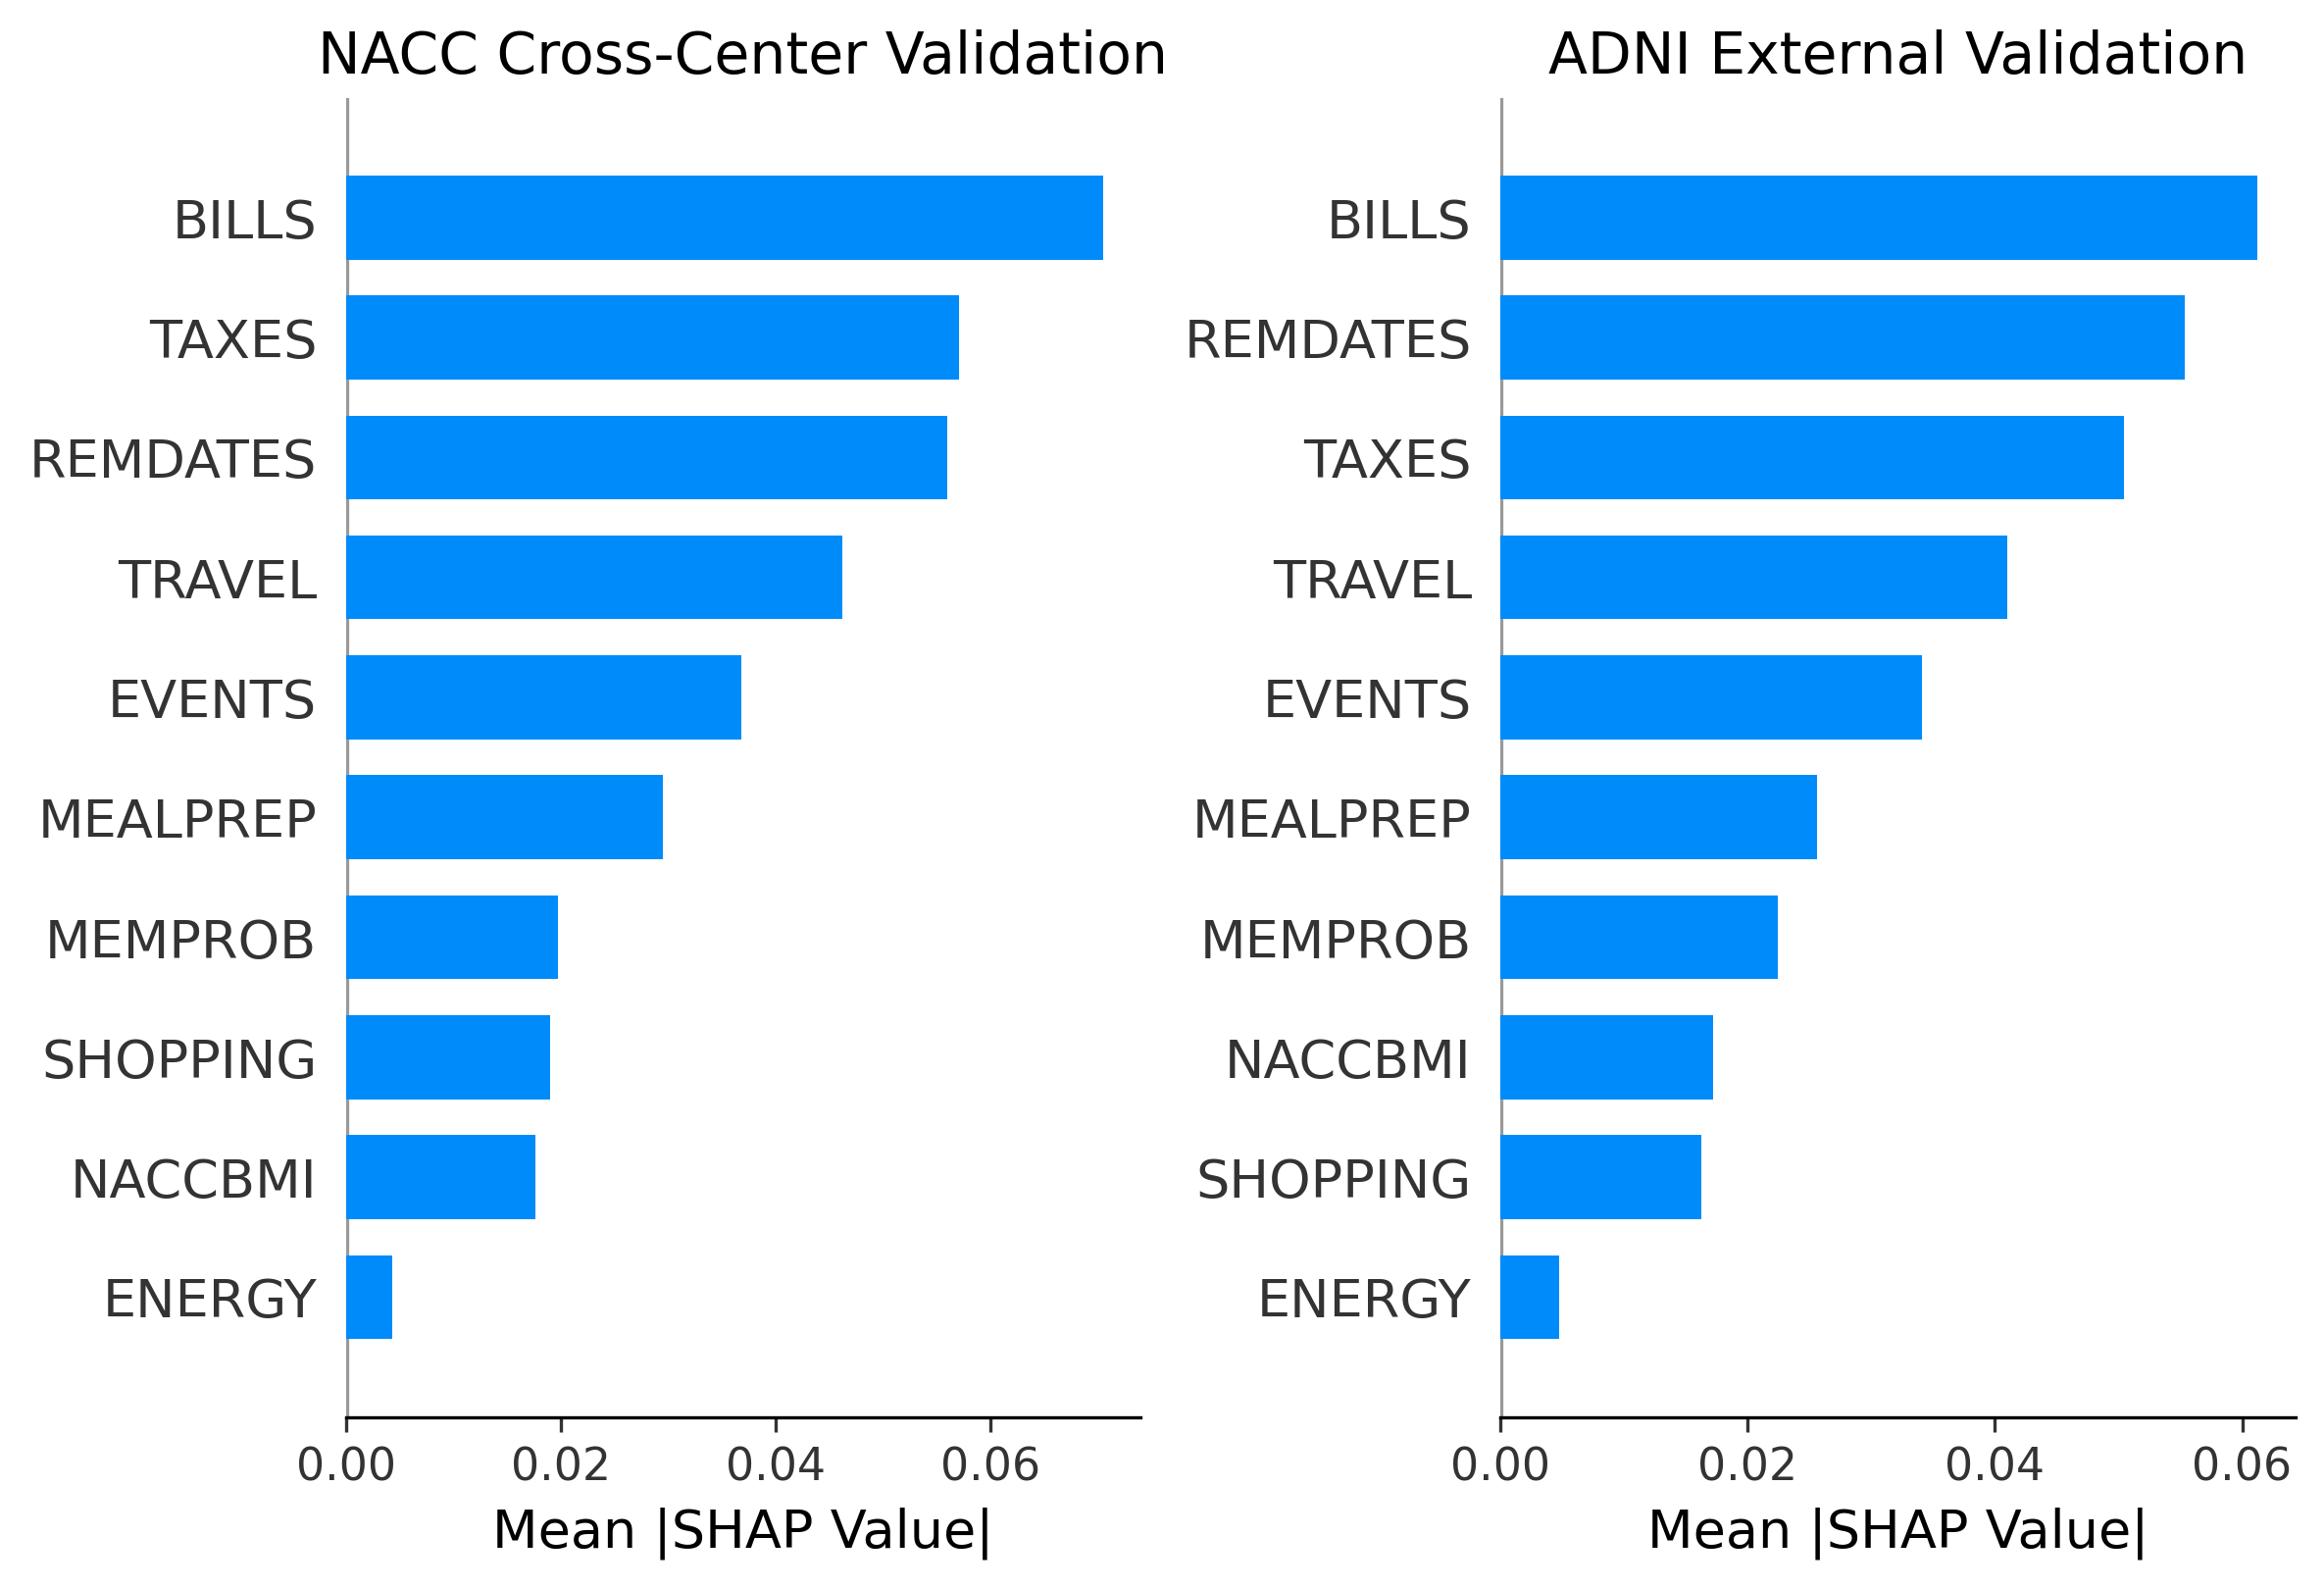
\includegraphics[width=1.0\textwidth]{figures/XAI/dementia_prediction_both_feature_importance_comparison.png}
    \caption{Feature importance in the NACC cross-center validation and the ADNI external validation for the future CIND vs. dementia prediction task}
    \begin{minipage}{\textwidth}
      \footnotesize \hl{The bars represent the mean absolute SHAP value of each feature, which ranks the contribution of the feature to the model prediction in the two validation datasets.}
    \end{minipage}
    \label{figure:cind_dementia_prediction_feature_importance}
\end{figure}

The local explanation of the selected LR model for the future prediction of CIND vs. dementia was assessed. The model was found to be capable of capturing heterogeneous impairment patterns that lead to similar diagnostic outcomes. For the correctly predicted dementia instances in Figure~\ref{figure:cind_dementia_prediction_pos_waterfall}, both \textit{Instance A} and \textit{Instance B} were predicted with similar probabilities of 54\% and 56\%, respectively. Both instances differ in the main risk factor that led to the prediction of dementia. In Instance A, the risk was primarily increased by the difficulty in assembling tax records (TAXES), while the difficulty in paying bills (BILLS) was a major risk factor in Instance B. Despite these differences, both instances shared a common underlying risk driven by memory problems (MEMPROB) and difficulty remembering dates (REMDATES).

\begin{figure}[ht]
    \centering
    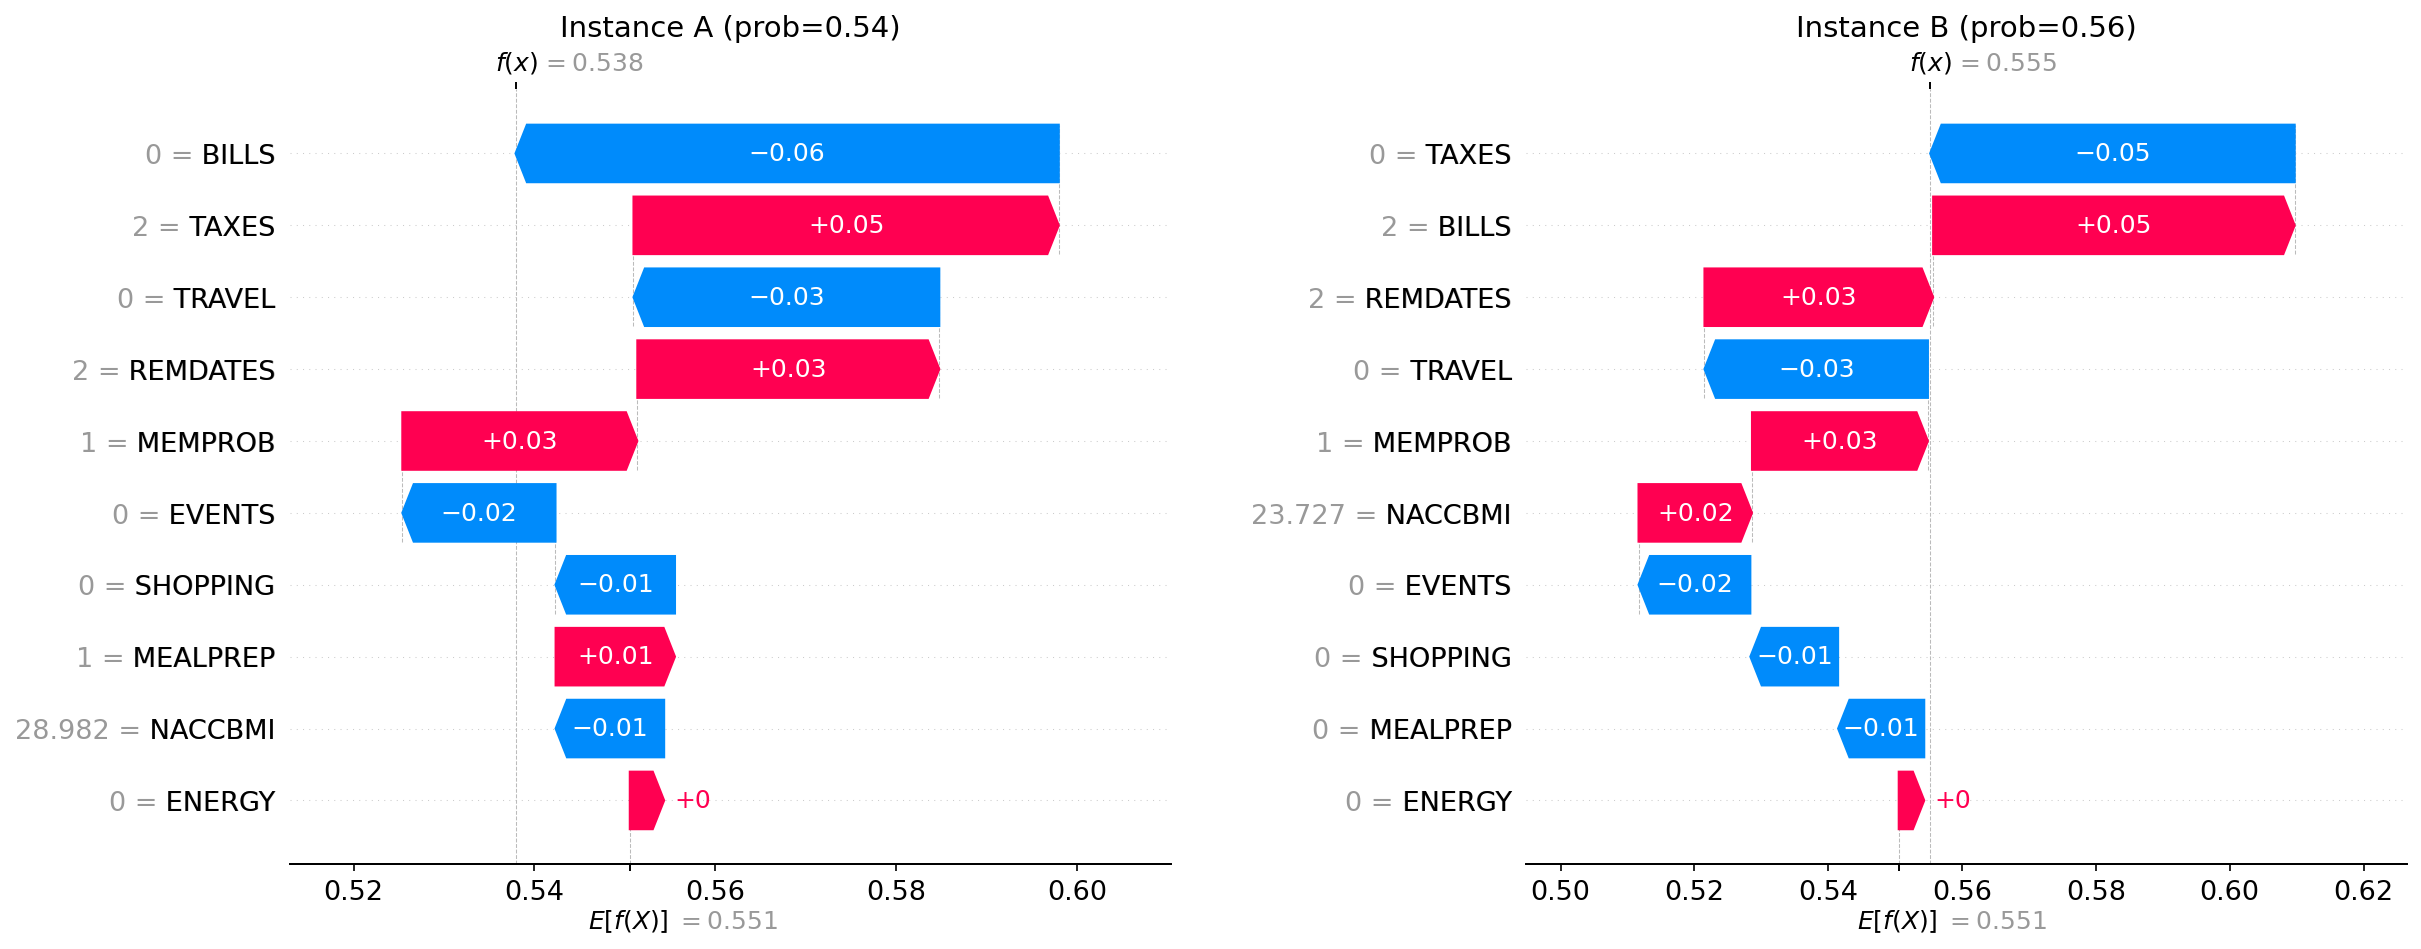
\includegraphics[width=1.0\textwidth]{figures/XAI/dementia_prediction_adni_true_positive_waterfall.png}
    \caption{SHAP waterfall plots for two instances correctly predicted as having risk of dementia within five years in future}
    \begin{minipage}{\textwidth}
      \footnotesize \hl{The plot shows how the value of each feature shifts the prediction from the base value to the final predicted probability for a single instance.}
    \end{minipage}
    \label{figure:cind_dementia_prediction_pos_waterfall}
\end{figure}

\newpage
Figure~\ref{figure:cind_dementia_prediction_neg_waterfall} shows the waterfall plots of two instances correctly predicted as CIND. \textit{Instance B} had a predicted probability of dementia lower than the classification threshold (43\% < 50\%). The low risk of dementia in this case was due to the ability to normally perform critical functional activities (REMDATES, TRAVEL, and EVENTS) and the absence of memory problems. This profile was quite different from Instance A, which had a similar predicted probability (44\%) despite difficulty traveling alone and reported memory problems. This is because executive functions related to financial management (BILLS, TAXES) were preserved as normal in Instance A.

\begin{figure}[ht]
    \centering
    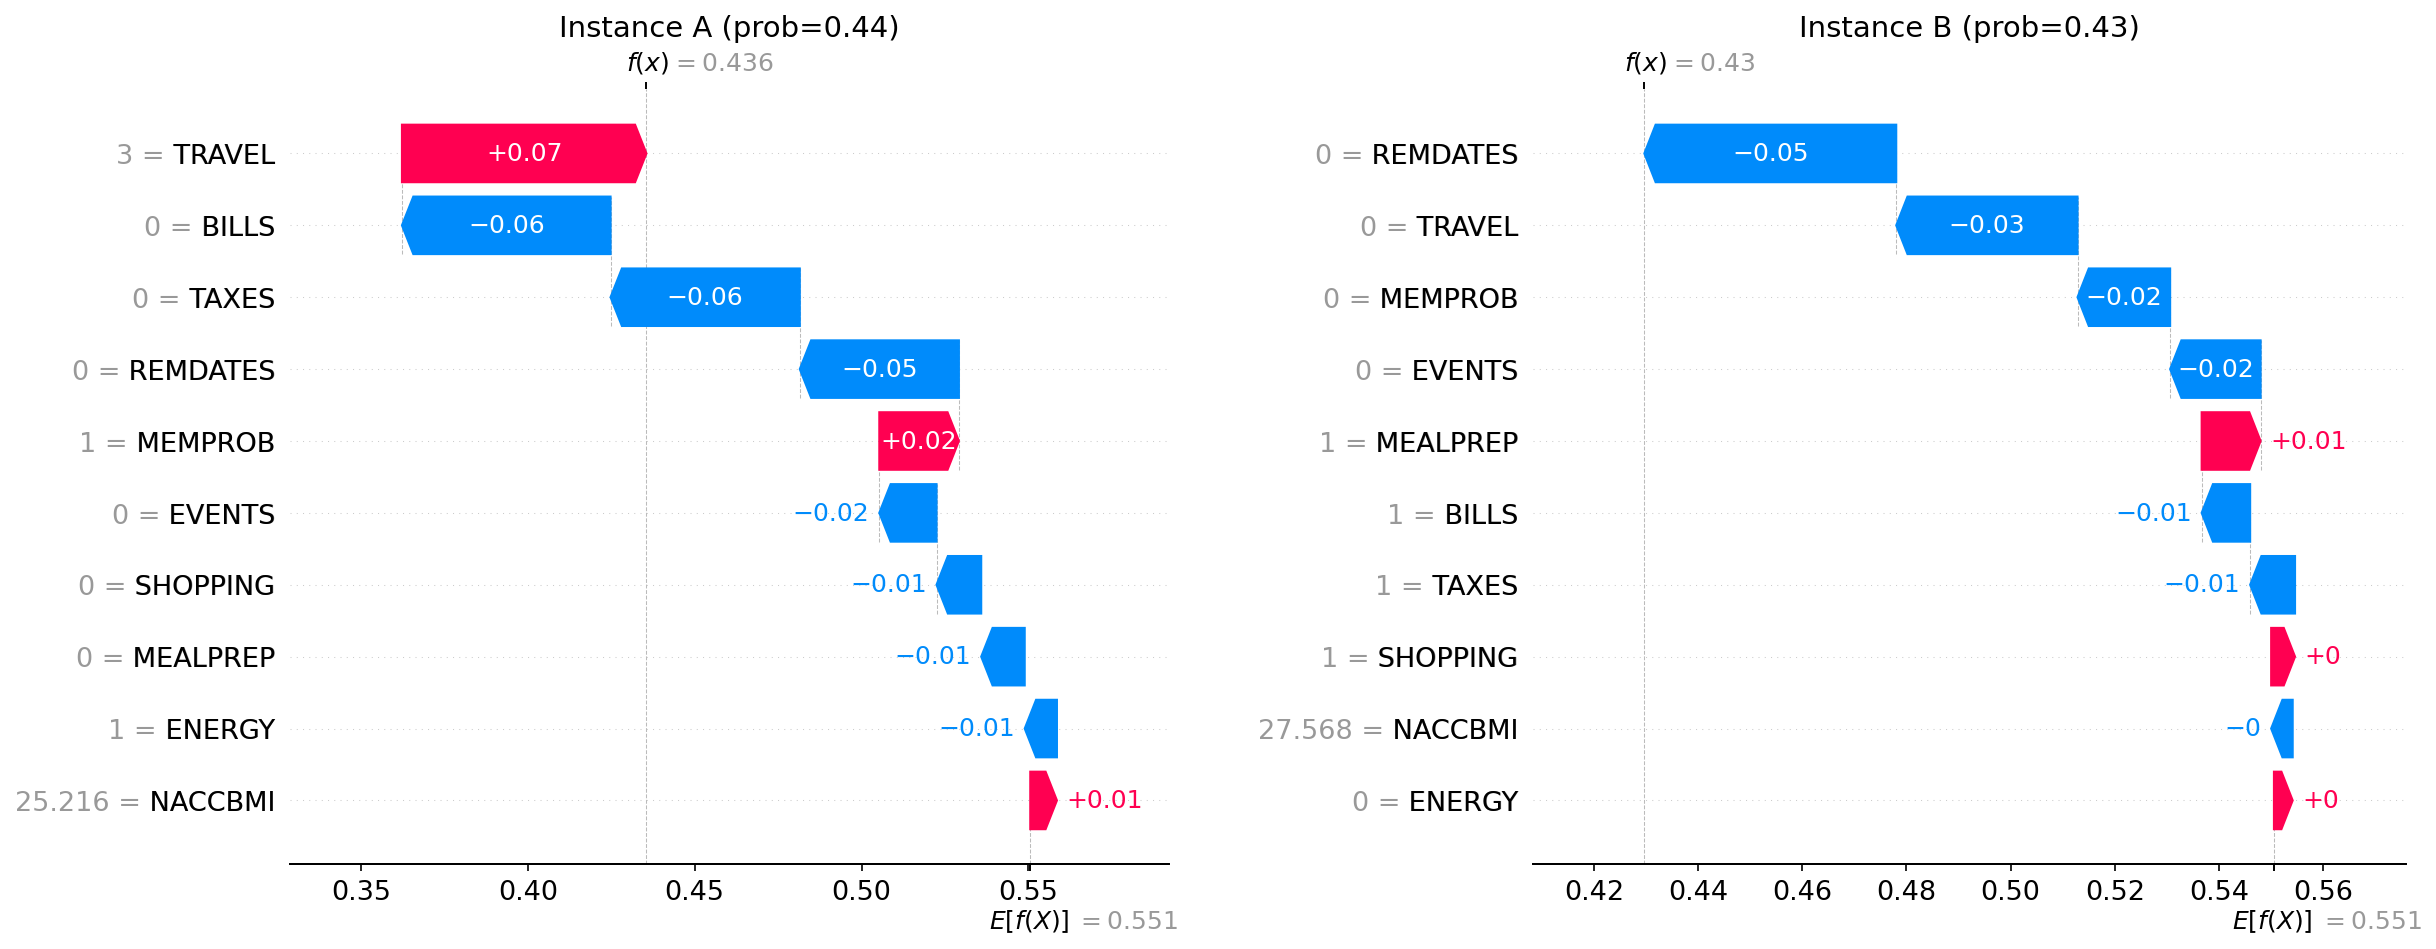
\includegraphics[width=1.0\textwidth]{figures/XAI/dementia_prediction_adni_true_negative_waterfall.png}
    \caption{SHAP waterfall plots for two instances correctly predicted as having risk of CIND within five years in future}
    \begin{minipage}{\textwidth}
      \footnotesize \hl{The plot shows how the value of each feature shifts the prediction from the base value to the final predicted probability for a single instance.}
    \end{minipage}
    \label{figure:cind_dementia_prediction_neg_waterfall}
\end{figure}

\newpage
For counterfactual explanation, using DiCE with the \acrshort{KD-Tree} (K-dimensional tree) search method failed to generate counterfactual examples for half of the ADNI samples. This is because of the limited size and sparsity of the training data in this task, which leaves large gaps between the data points in the KD-Tree structure. As a result, the algorithm was unable to find enough similar instances to construct valid counterfactuals. To overcome this challenge, DiCE with random search was utilized in this task. Random search is not affected by the sparsity of the training data because it generates new synthetic examples by exploring the range of possible feature values to obtain the required outcome.

The DiCE random search method managed to generate counterfactual explanations for risk prevention for only 86.8\% of the ADNI external data instances. This rate is lower than the rates of the other classification and prediction tasks. However, DiCE in this task was able to provide up to five different counterfactual examples for around 72\% of the instances, significantly exceeding the results of the NC vs. CI prediction task. The results of the counterfactual explanation for the future prediction of CIND vs. dementia are presented in Figure~\ref{figure:cind_dementia_prediction_dice_stat}. Analysis of feature changes indicates that the effort required to prevent the risk of dementia is low, with a median of two feature changes. In fact, more than half of the generated counterfactuals (52.8\%) required modifying only one or two risk factors (features). The counterfactual explanation results of the NACC cross-center validation, which are presented in Figure~\ref{figure:dice-nacc-task4-apdx} in the Appendix, showed a similar pattern with a higher percentage of instances without counterfactual examples.

\begin{figure}[ht]
    \centering
    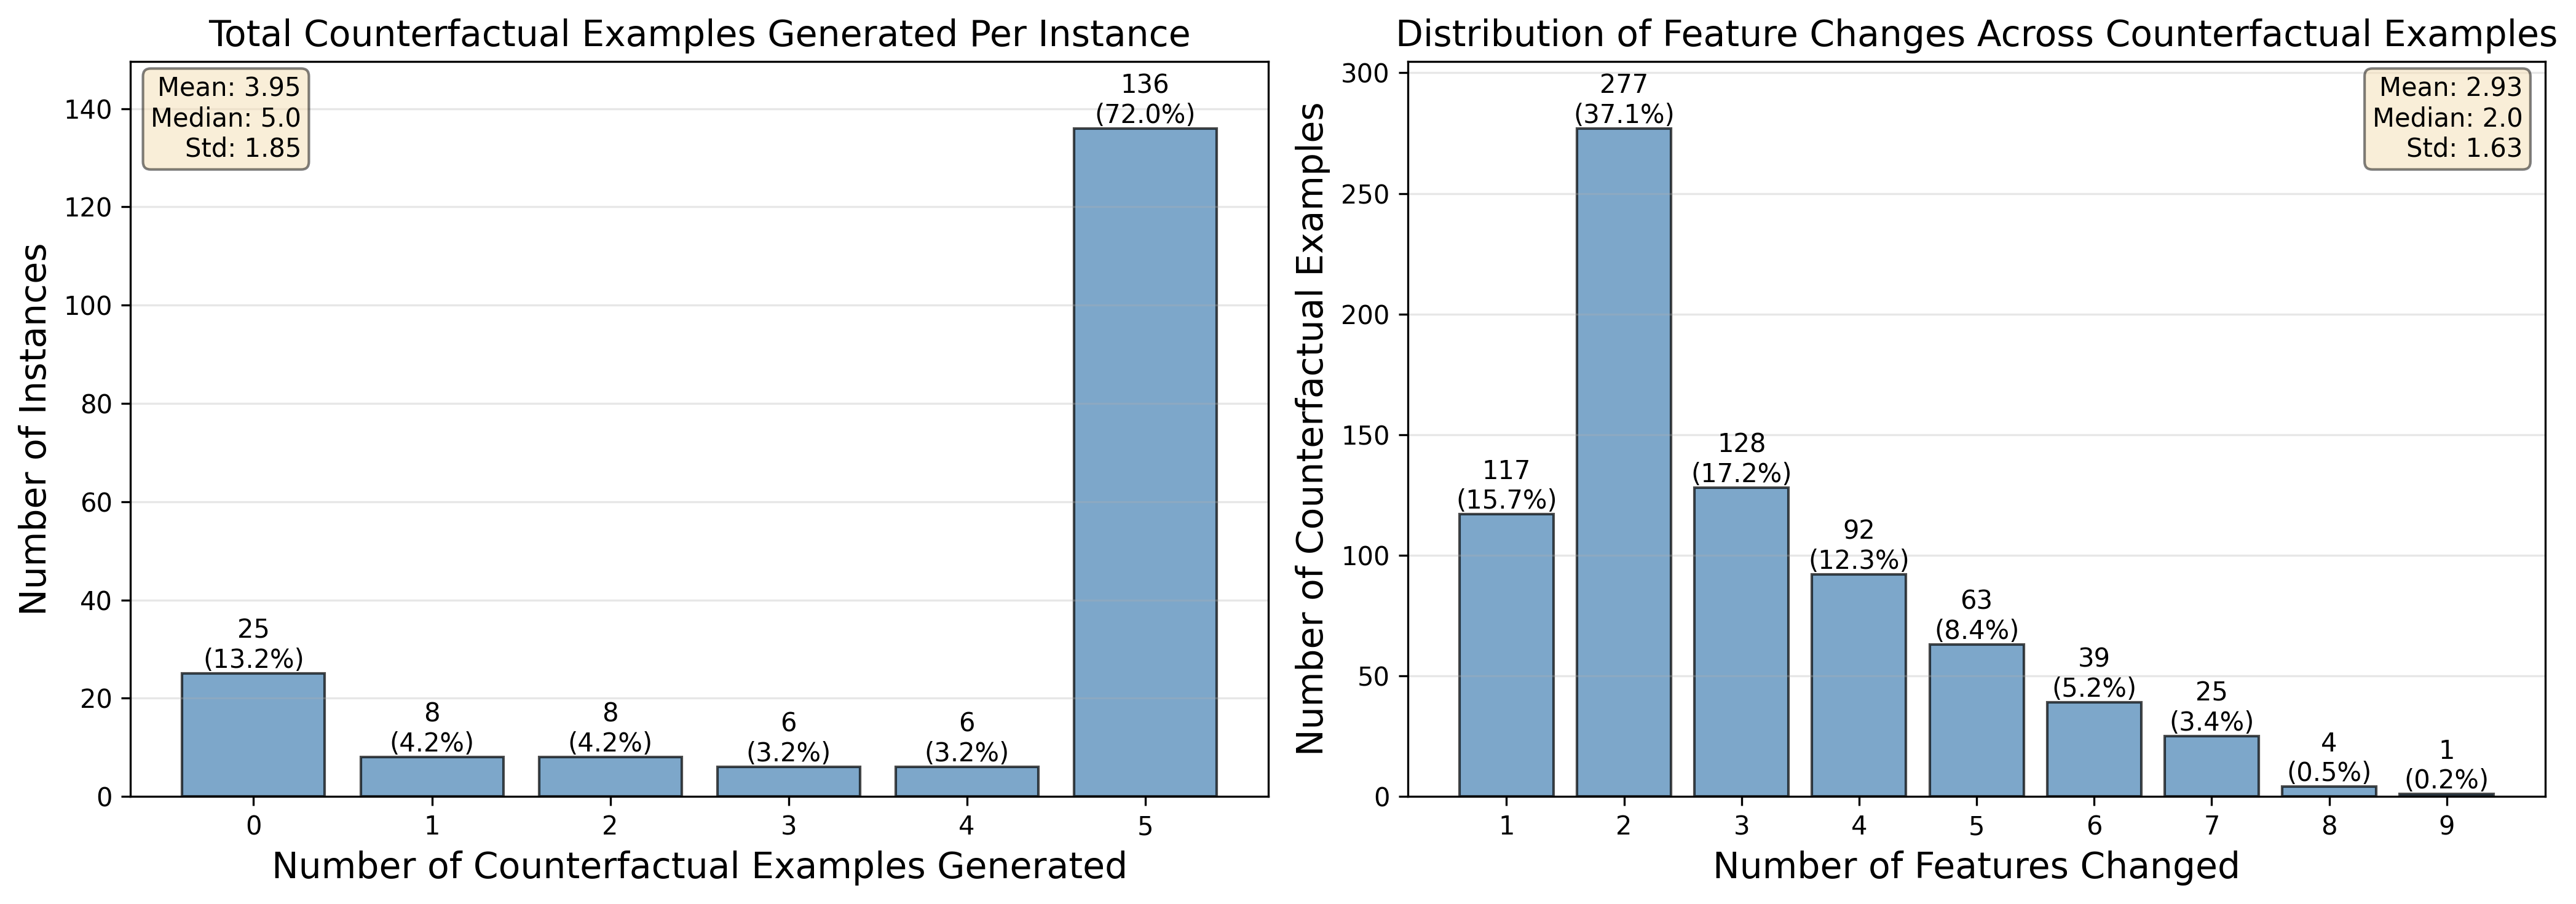
\includegraphics[width=1.0\textwidth]{figures/XAI/dementia_prediction_adni_random_dice_stats.png}
    \caption{Summary of generated counterfactual examples for changing predicted risk from dementia to CIND}
    \label{figure:cind_dementia_prediction_dice_stat}
\end{figure}

The features that should be prioritized for the prevention of the risk of dementia are ranked in Figure~\ref{figure:cind_dementia_prediction_dice_feature_importance}. The ability to remember dates and appointments (REMDATES) was the most frequently modified feature (54\%). Financial management activities from FAQ were also important, with changes in paying bills (BILLS) and  handling taxes (TAXES) contributing to 50\% and 47\% of the generated counterfactual examples, respectively. In contrast, body mass index (NACCBMI), self-reported memory problems (MEMPROB), energy levels (ENERGY) and other functional activities (MEALPREP and SHOPPING) changed in 20\% or fewer of the counterfactual examples generated. Table~\ref{table:cfe-adni-task4-apdx} in the appendix illustrates counterfactual examples generated for a random subject with a future risk of dementia to reverse the estimated outcome to CIND.

\begin{figure}[ht]
    \centering
    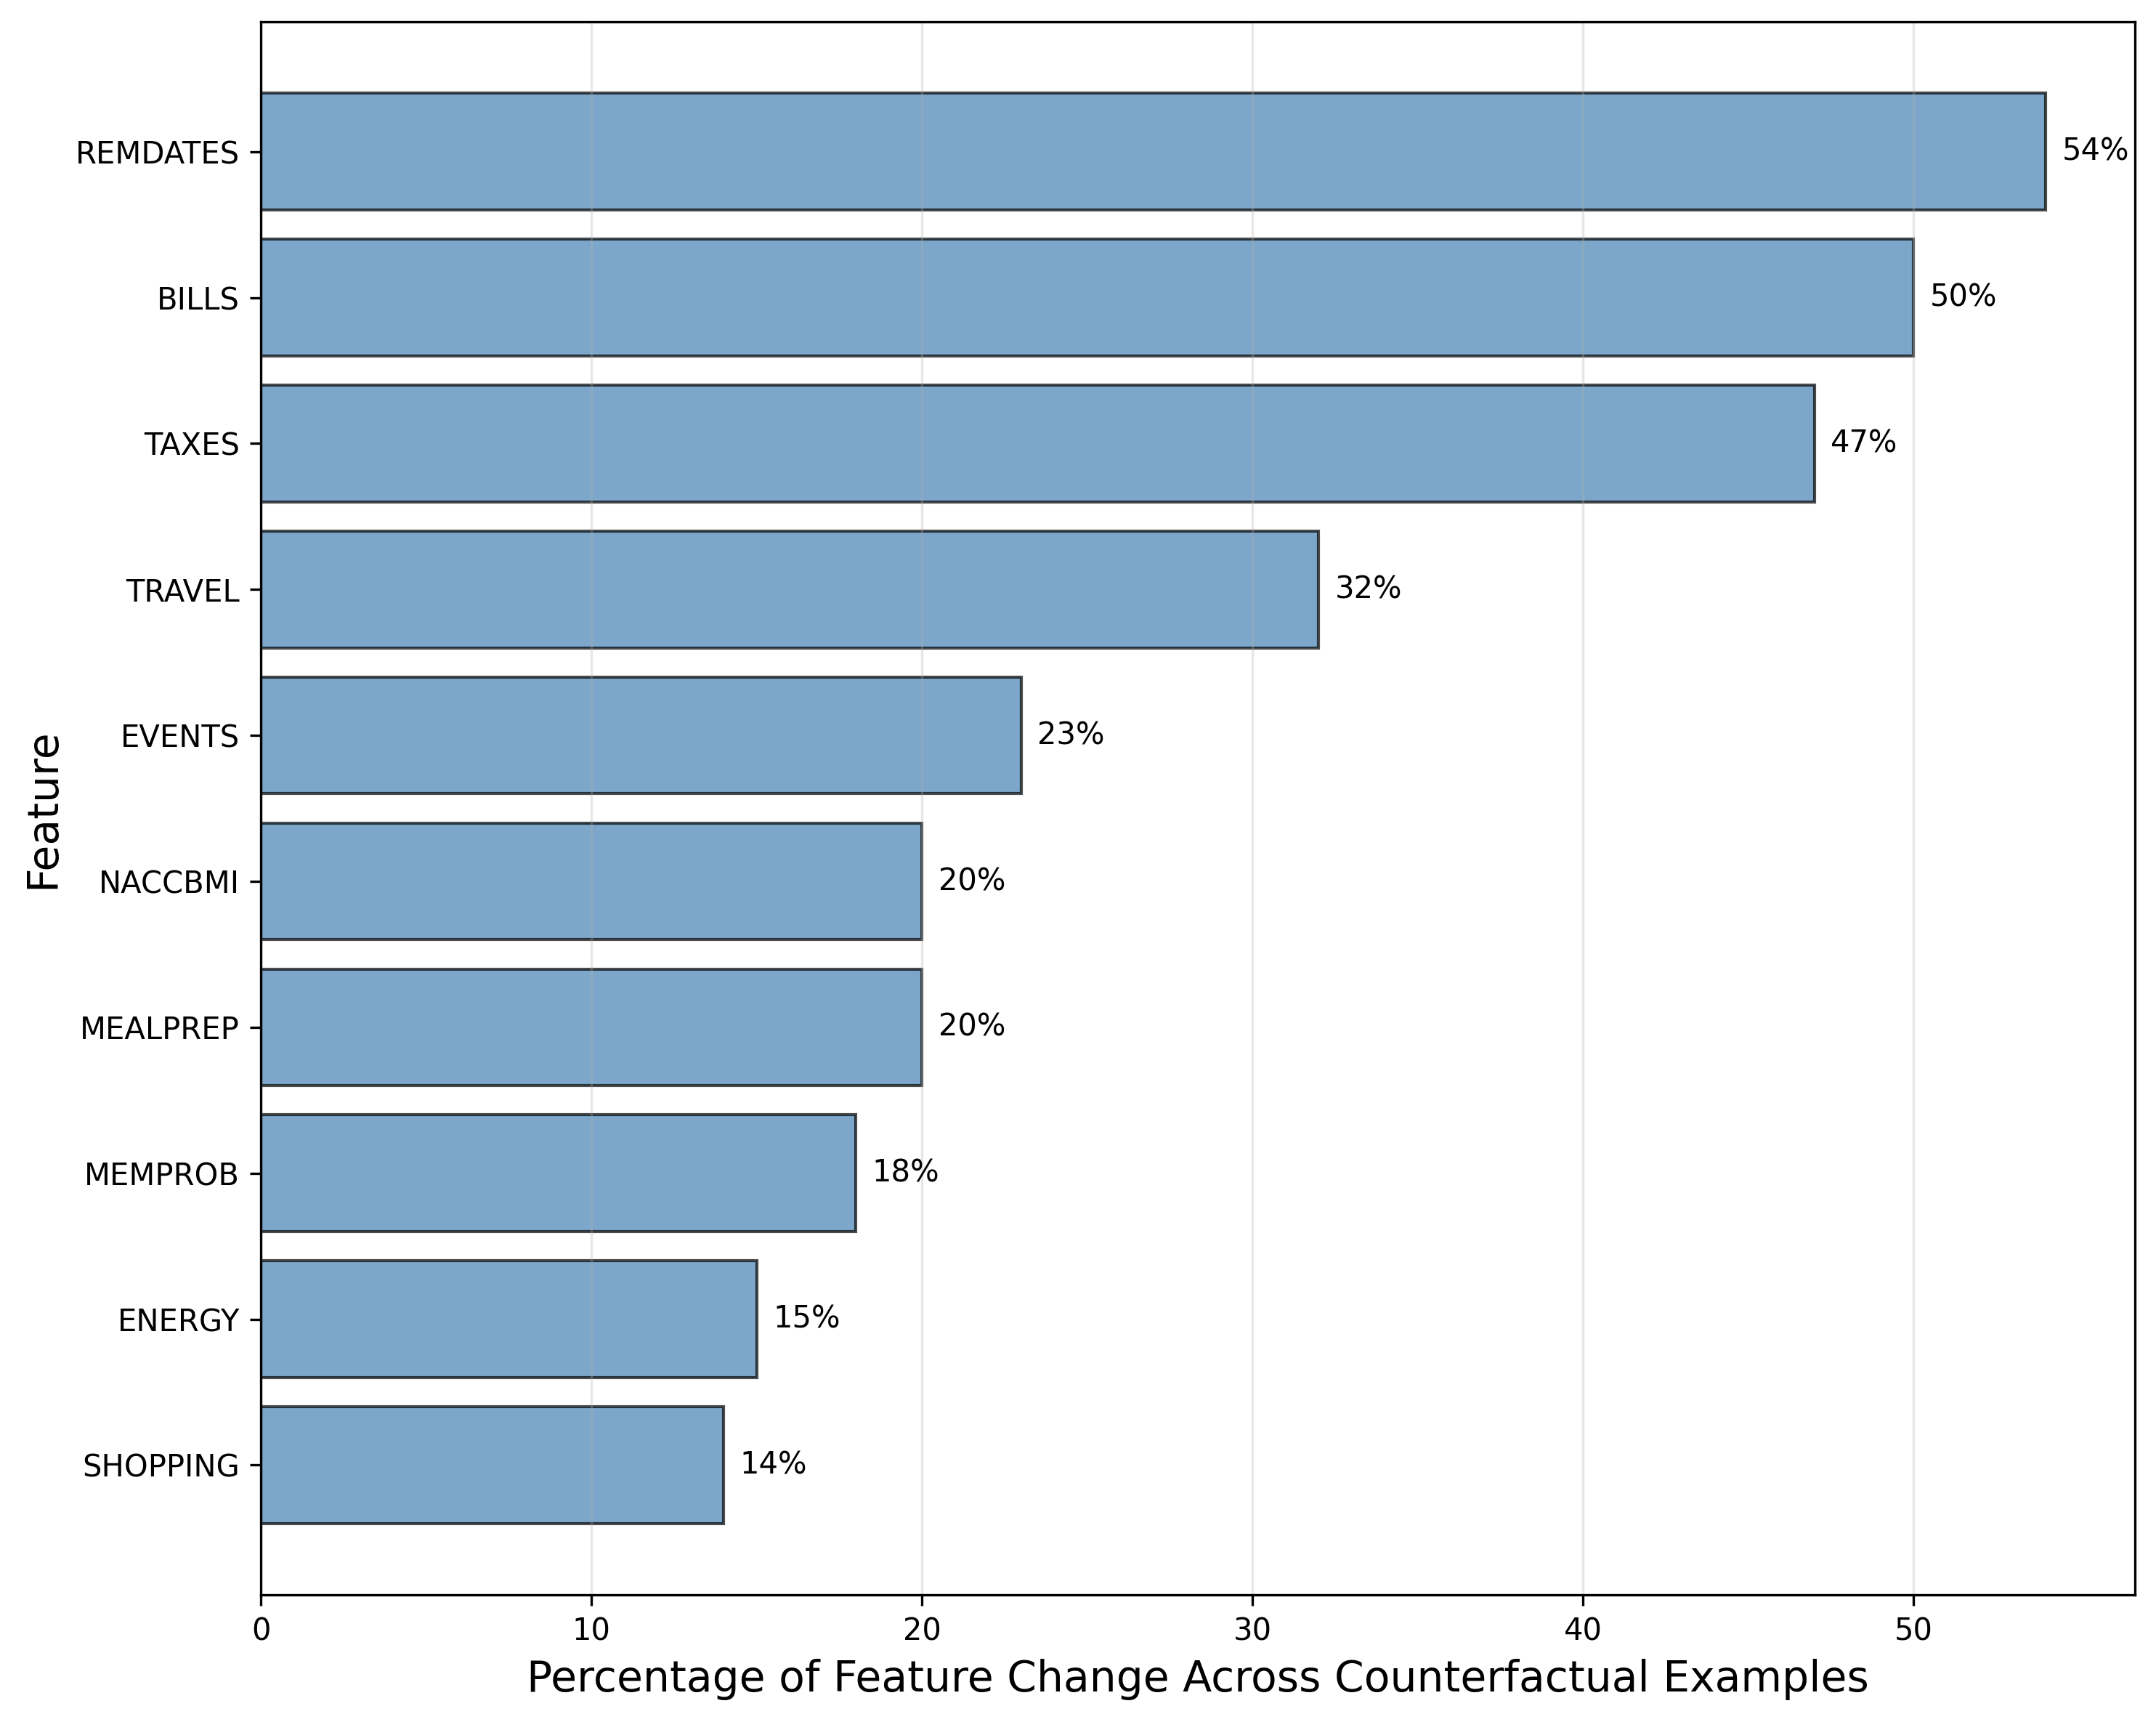
\includegraphics[width=1.0\textwidth]{figures/XAI/dementia_prediction_adni_random_dice_global_importance.png}
    \caption{Feature importance ranking based on counterfactual explanations for the future CIND vs. dementia prediction task}
    \begin{minipage}{\textwidth}
      \footnotesize The features are ranked based on the percentage of times they were modified to generate valid counterfactual examples. The rank highlights the most critical features for risk intervention.
    \end{minipage}
    \label{figure:cind_dementia_prediction_dice_feature_importance}
\end{figure}

\section{Cognitive Impairment Subtype Classification Results}
This section addresses the third research objective: the classification of cognitive impairment subtypes, specifically Alzheimer's Disease (\acrshort{AD}) vs. non-AD etiologies. As hypothesized in the introduction, this task is expected to be the most challenging due to the expected major feature overlap between different types of cognitive impairment.

\subsection{Feature Selection Results}
The evaluation of the feature selection method was applied to this classification task. The proposed method was compared with the baseline and the Boruta method. The results of the comparison using the standard RF model are presented in Table~\ref{table:fs-task5}.

\begin{table}[!ht]
    \centering
    \caption{Comparison of feature selection methods for the AD vs. non-AD classification task}
    \begin{tabular}{|c|c|c|c|c|}
    \hline
        Method & Number of Features & G-mean & Fitness Score & F1 \\ \hline
        Baseline & 77 & 0.730 & 0.608 & 0.988 \\ \hline
        Boruta & 12 & 0.699 & 0.723 & 0.955 \\ \hline
        \textbf{Proposed Method} & \textbf{8} & \textbf{0.668} & \textbf{0.706} & \textbf{0.931} \\ \hline
        \multicolumn{5}{p{400pt}}{\footnotesize \hl{F1: Fisher's discriminant ratio (feature overlap measure), Fitness Score: combined score balancing performance and feature reduction, G-mean: geometric mean score.}}
    \end{tabular}
    \label{table:fs-task5}
\end{table}

The results confirm the high difficulty of this task, with lower G-mean scores in all methods compared to the scores obtained in the cognitive status classification and prediction tasks. The complexity can be noticed from the high F1 class overlap scores. The baseline achieved the highest G-mean (0.730) but the lowest fitness score (0.608) because it used all 77 features. The proposed method was the most successful in reducing complexity and improving efficiency by selecting only eight features. This subset achieved the lowest F1 class overlap score (0.931) and had a model training speed that was 2.5 times faster than the baseline.

\newpage
The Boruta method obtained the highest fitness score of 0.723 by selecting 12 features and producing an RF model with a G-mean of 0.699. This resulted in a higher G-mean score than the proposed method (0.668). Given this finding, a supplementary analysis was carried out to assess the robustness of these feature sets. The performance of the three feature sets was evaluated using two other common classifiers: LR and SVM. The G-mean scores of the three models are presented in Table~\ref{table:fs-task5-more-models}.

\begin{table}[!ht]
    \centering
    \caption{Comparison of feature selection methods in the AD vs. non-AD classification task based on G-mean performance across different models}
    \begin{tabular}{|c|c|c|c|c|}
    \hline
        Method & RF (G-mean) & LR (G-mean) & SVM (G-mean) \\ \hline
        Baseline (77 features) & 0.730 & 0.724 & 0.736 \\ \hline
        Boruta (12 features) & 0.699 & 0.687 & 0.705 \\ \hline
        Proposed Method (8 features) & 0.668 & 0.691 & 0.701 \\ \hline
        \multicolumn{4}{p{400pt}}{\footnotesize \hl{G-mean: geometric mean score, LR: logistic regression, RF: random forest, SVM: support vector machines.}}
    \end{tabular}
    \label{table:fs-task5-more-models}
\end{table}

The G-mean results show that the performance of the selected feature sets is model-dependent. While the baseline performed best overall, the comparison between the proposed method and the Boruta method is more interesting. The 12-feature set from the Boruta method performed best with the RF model, but the 8-feature set from the proposed method achieved a higher G-mean when using the LR model (0.691 vs. 0.687). Both methods were highly comparable when using the SVM model (0.701 vs. 0.705).

The analysis of the feature selection demonstrates that the proposed method is capable of selecting the smallest set of features that could reduce the complexity of the data and increase the computational efficiency of the model. Moreover, the selected features are highly robust and generalizable across different types of classification algorithms.

The eight features that were selected by the proposed method for this CI subtype classification task are listed in Table~\ref{table:features-task5}. 6 out of the 8 features are related to the Clinical Dementia Rating (\acrshort{CDR}) scale. The list also includes the subject's age and a single feature from the FAQ. More details of the selected features and their correlation results can be found in section \ref{sec:feature-selection-apdx} in the appendix.

\begin{table}[h!]
\centering
\caption{List of selected features for the AD vs. non-AD classification task}
\label{table:features-task5}
\begin{tabular}{ccc}
\toprule
\textbf{Feature Code} & \textbf{Feature Description} & \textbf{Feature Category} \\
\midrule
NACCAGE & Age & Demographics \\
MEMORY & Memory & CDR \\
ORIENT & Orientation & CDR \\
JUDGMENT & Judgment \& Problem Solving & CDR \\
COMMUN & Community Affairs & CDR \\
HOMEHOBB & Home \& Hobbies & CDR \\
PERSCARE & Personal Care & CDR \\
REMDATES & Remember dates and appointments & FAQ \\
\bottomrule
\end{tabular}
\end{table}

\subsection{Data Resampling Results}
\label{sec:resampling_results_ro3}
The results of the data resampling method of the AD vs. non-AD classification task are presented in this section. Differentiating AD from non-AD disorders using accessible data was hypothesized to be a challenging task. The complexity of the training data could confirm this. According to the analysis of the class imbalance and overlap, this task presented the most severe data complexity of all tasks in this study. The AD examples are 1.35 more than the minority non-AD examples. Additionally, a very high class overlap was observed with 0.323 instance-level class overlap (kDN) and 0.511 structural class overlap (N1). The analysis of borderline example measures also showed that the minority non-AD class was deeply embedded in the overlapped region, with 46\% of its examples identified as borderline, compared to 34\% for the majority class (AD). The distribution of the target classes in the NACC UDS is presented in Figure~\ref{fig:nacc-data-stat} in the appendix.

This combination of high overlap and a higher proportion of borderline minority examples led to the selection of the ENN + KMeansSMOTE method, as specified by the decision algorithm (Algorithm \ref{alg:data-resampling}). ENN was first applied to clean overlapped instances, and then KMeansSMOTE was used to increase the minority class occurrence in safe clusters instead of adding more minority examples around the already complex decision boundary. The performance of this selected strategy was then assessed against the baseline and standard resampling methods. Table~\ref{table:ad_nonad_resampling} lists the results of this comparison. The results are also illustrated in Figure~\ref{figure:ad_nonad_resampling_perf}.

As shown in Table~\ref{table:ad_nonad_resampling}, the severe overlap in the baseline data resulted in a low balanced performance (G-mean = 0.668). This is because the RF model was unable to accurately classify the minority non-AD class (recall = 0.626). It is important to note that oversampling methods like ROS and SMOTE were ineffective as they failed to reduce the class overlap. Although these methods resulted in an improvement in non-AD recall, they lead to a considerable decrease in AD recall from 0.714 to 0.666 in ROS and 0.677 in SMOTE. This dramatic change in the performance of the RF model in both classes was also observed in the RUS method, where the non-AD recall increased to the highest score of  0.712 while the AD recall dropped by 7.5 percentage points to the lowest score of 0.639. The application of the RUS method resulted in an increase in the structural class overlap (N1) to 0.522. 

\begin{table}[!ht]
    \centering
    \caption{Performance comparison of resampling methods for the AD vs. non-AD classification task using a random forest model}
    \begin{tabular}{|c|c|c|c|c|c|}
    \hline
        Method & G-mean & Recall (AD) & Recall (non-AD) & kDN & N1 \\ \hline
        Baseline & 0.668 & 0.714 & 0.626 & 0.323 & 0.511 \\ \hline
        ROS & \makecell{0.673 \\ {\small \hl{(p = 0.125)}}} & 0.666 & 0.681 & 0.317 & 0.503 \\ \hline
        RUS & \makecell{0.674 \\ {\small \hl{(p = 0.157)}}} & 0.639 & \textbf{0.712} & 0.306 & 0.522 \\ \hline
        SMOTE & \makecell{0.674 \\ {\small \hl{(p = 0.011)}}} & 0.677 & 0.671 & 0.315 & 0.491 \\ \hline
        \makecell{\textbf{ENN +} \\ \textbf{KMeansSMOTE}} & \makecell{\textbf{0.710} \\ {\small \hl{(p = 0.001)}}} & \textbf{0.729} & 0.692 & \textbf{0.021} & \textbf{0.125} \\ \hline
        \multicolumn{6}{p{400pt}}{\footnotesize \hl{G-mean: geometric mean score, kDN: k-disagreeing neighbors (instance-level class overlap), N1: structural class overlap, Recall: per-class recall.}}
    \end{tabular}
    \label{table:ad_nonad_resampling}
\end{table}

\begin{figure}[ht]
\centering
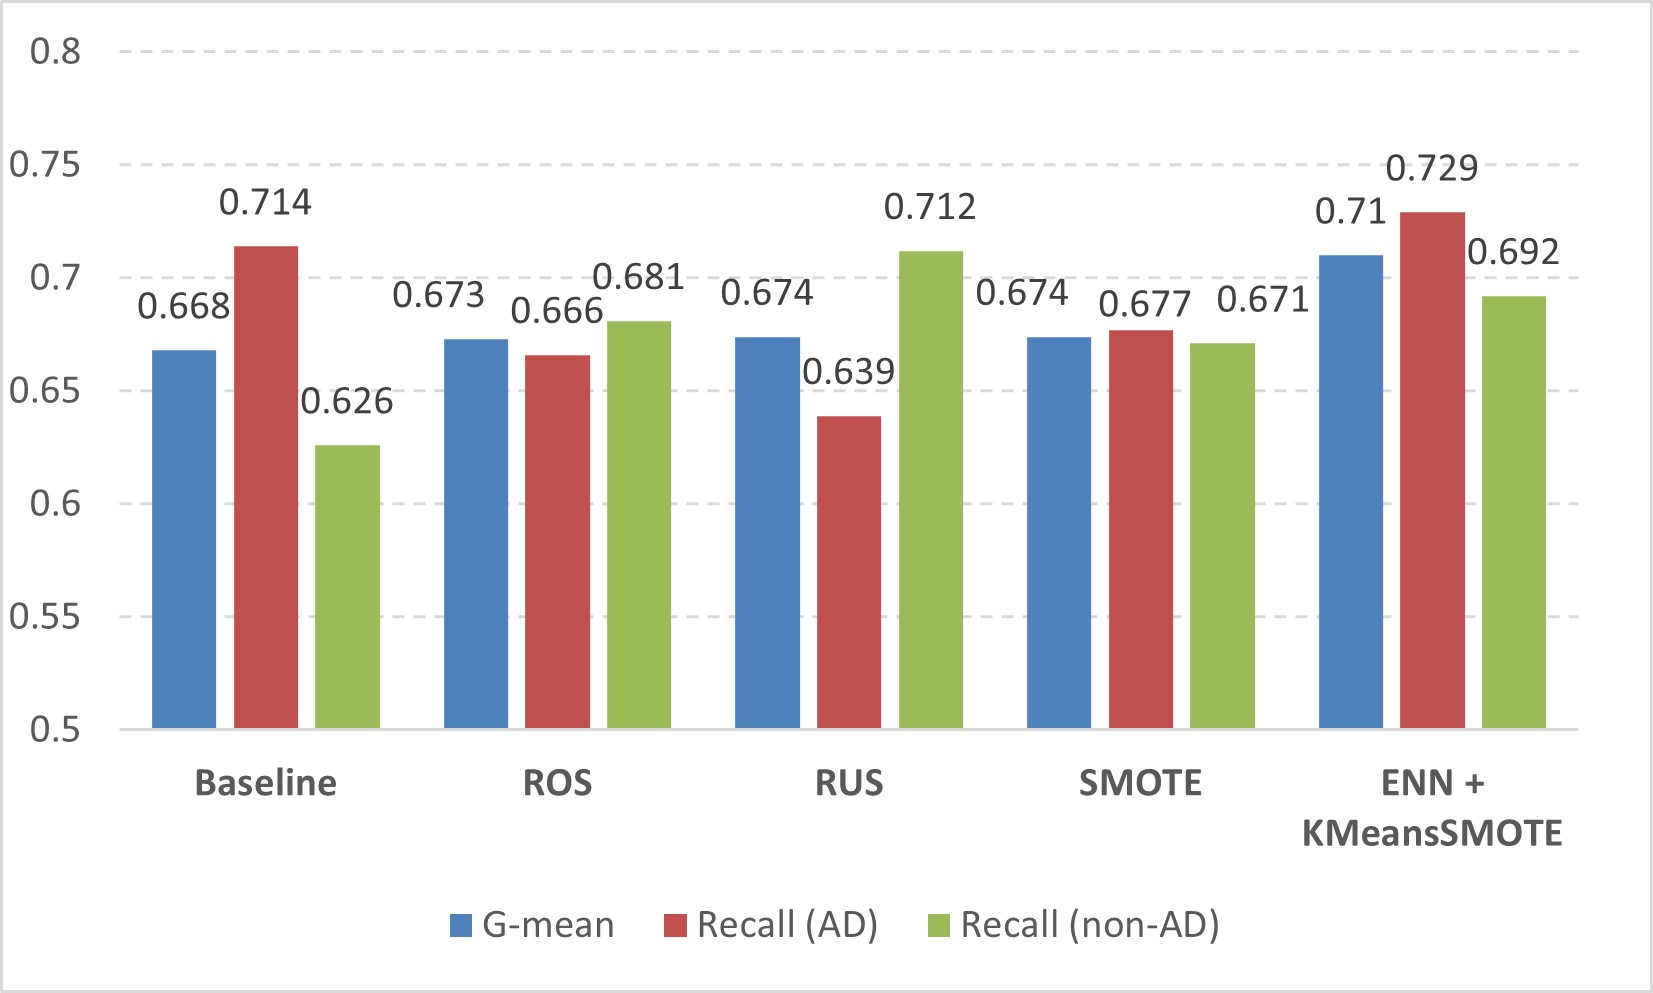
\includegraphics[width=1\textwidth]{figures/data-resampling-task5.jpg}
\caption{Model performance comparison of data resampling methods for the AD vs. non-AD classification task}
\label{figure:ad_nonad_resampling_perf}
\end{figure}

In contrast, the selected ENN + KMeansSMOTE method produced the most effective and balanced RF model. It was the only method that successfully addressed the data complexity by totally reducing both instance-level and structural class overlap. As a result, this method achieved the highest G-mean of 0.710. This is more than 4 percentage points of improvement from the baseline model. It did this by significantly improving the recall of the minority non-AD class to 0.692 while achieving the highest recall for the AD class at 0.729. This confirms that for this highly complex task, a specialized strategy that first cleans the overlap and then systematically resamples the minority class is necessary to achieve a balanced and effective classification model. \hl{The G-mean improvement of the proposed ENN + KMeansSMOTE method over the baseline was highly significant (p = 0.001) and was the strongest result among all the evaluated methods, which confirms the effectiveness of the proposed strategy in this complex task.}

\subsection{Model Fine-tuning and Selection Results}
The final model fine-tuning and selection process was also applied to the CI subtype classification task. The results of optimizing and selecting the best model that distinguishes between AD and non-AD disorders are outlined in this section.

The cost-effective selection algorithm (Algorithm \ref{alg:model-selection}) was again utilized to identify the most suitable models. The G-mean metric was used to evaluate the performance of the models with a balanced evaluation of both classes. The selection algorithm successfully identified sets of hyperparameters that offered significant speed improvements for most models. The training speed of the LR and KNN models improved by around 1.3 times while maintaining the same G-mean scores as the best-performing models. The highest gain in prediction speed was achieved by the KNN model (2.39 times), followed by the LightGBM model (1.49 times) and the LR model (1.2 times). The performance and throughput of the five optimized models are presented in Table~\ref{table:task5_finalists_models}.

\begin{table}[!ht]
\centering
\caption{Summary of fine-tuned models for the AD vs. non-AD Classification Task}
\label{table:task5_finalists_models}
\newcolumntype{C}{>{\centering\arraybackslash}X}
    \begin{tabularx}{\textwidth}{|C|C|C|C|}
        \hline
        \textbf{Model} &
        \textbf{G-mean\newline(95\% CI)} &
        \textbf{Training Throughput (Gain)\textsuperscript{1}} &
        \textbf{Prediction Throughput (Gain)\textsuperscript{1}} \\
        \hline
        KNN &
        0.682 ($\pm 0.006$) &
        $778,285$ $(1.31\times)$ &
        $47,963$ $(2.39\times)$ \\
        \hline
        LR &
        0.702 ($\pm 0.005$) &
        $1,123,435$ $(1.34\times)$ &
        $19,910,963$ $(1.20\times)$ \\
        \hline
        LightGBM &
        0.699 ($\pm 0.005$) &
        $192,613$ $(1.03\times)$ &
        $1,086,848$ $(1.49\times)$ \\
        \hline
        RF &
        0.705 ($\pm 0.005$) &
        $29,743$ $(1.04\times)$ &
        $157,279$ $(1.04\times)$ \\
        \hline
        SVM &
        0.709 ($\pm 0.006$) &
        $1,157$ &
        $7,466$ \\
        \hline
        \multicolumn{4}{p{400pt}}{\footnotesize \textsuperscript{1}\hl{Training throughput is reported in training samples per second, and prediction throughput in predictions per second.} Gain is calculated as the ratio of the selected model’s throughput to the benchmark model’s throughput. Values indicate the factor by which training and prediction speed have improved. Gain is not presented when the selected model is the benchmark model.}
    \end{tabularx}
\end{table}

A final assessment was conducted to select only one best model. Performance, efficiency, and interpretability were the focus of this assessment. The LR model was selected as the best model for its ability to provide a cost-effective classification. Regarding performance, the LR model's G-mean of 0.702 is statistically comparable to the highest-performing SVM (0.709) and RF (0.705) models. Second, on top of high performance, the LR model is also extremely efficient. This efficiency significantly exceeded all models. Even though the SVM model had the highest G-mean, it was the slowest model overall. Finally, the linear nature of the LR model ensures high interpretability, which is a core objective for this study. In contrast, the SVM and RF models are significantly more computationally intensive. In addition, they are more complex to explain. Therefore, the best trade-off of accuracy, high speed, and easy interpretability is offered by the LR model. Table~\ref{table:lr-fine-tune-task5-apdx} in the appendix presents the hyperparameter fine-tuning results of the LR model.

In summary, the model fine-tuning and selection process has been successfully completed for all five classification tasks. The findings consistently show that the LR models are the most cost-effective across all tasks. By achieving performance that is statistically comparable to more complex models, such as RF and SVM, while offering substantial advantages in computational speed and high interpretability, the LR model successfully addresses the core research objectives concerning cost-effectiveness and explainability. The following sections analyze the external validation and model explainability of the selected LR models.

\subsection{Model Performance in External Validation}
The generalizability of the selected LR model for the AD vs. non-AD classification task was tested on the holdout NACC cross-center testing dataset, which contains unseen data from different research centers. The details of the validation method are provided in section \ref{sec:model-validation}.

The performance of the model in the NACC cross-center validation was analyzed and compared to the model's performance in the internal CV. The results are listed in Table~\ref{tab:ad_nonad_results}. Additionally, the ROC curves for the internal CV and the NACC cross-center validation are illustrated by Figure~\ref{fig:ad_nonad_roc}.

\begin{table}[!ht]
    \centering
    \caption{Performance of the selected logistic regression model in internal and external validation for the AD vs. non-AD classification task}
    \label{tab:ad_nonad_results}
    \begin{tabular}{|c|c|c|}
        \hline
        \textbf{Metric} & \textbf{Internal CV} & \textbf{NACC Cross-center Validation} \\
        \hline
        AUC & \makecell{0.702 \\ {\small \hl{(0.698--0.706)}}} & \makecell{0.670 \\ {\small \hl{(0.658--0.681)}}} \\ \hline
        G-mean & 0.702 & 0.670 \\ \hline
        Sensitivity & 0.689 & 0.679 \\ \hline
        Specificity & 0.714 & 0.660 \\ \hline
        F1-score & 0.725 & 0.706 \\
        \hline
        \multicolumn{3}{p{400pt}}{\footnotesize \hl{AUC: area under the curve, F1-score: harmonic mean of precision and recall, G-mean: geometric mean score, Sensitivity: recall of the AD class, Specificity: recall of the non-AD class.}}
    \end{tabular}
\end{table}

\begin{figure}[ht]
    \centering
    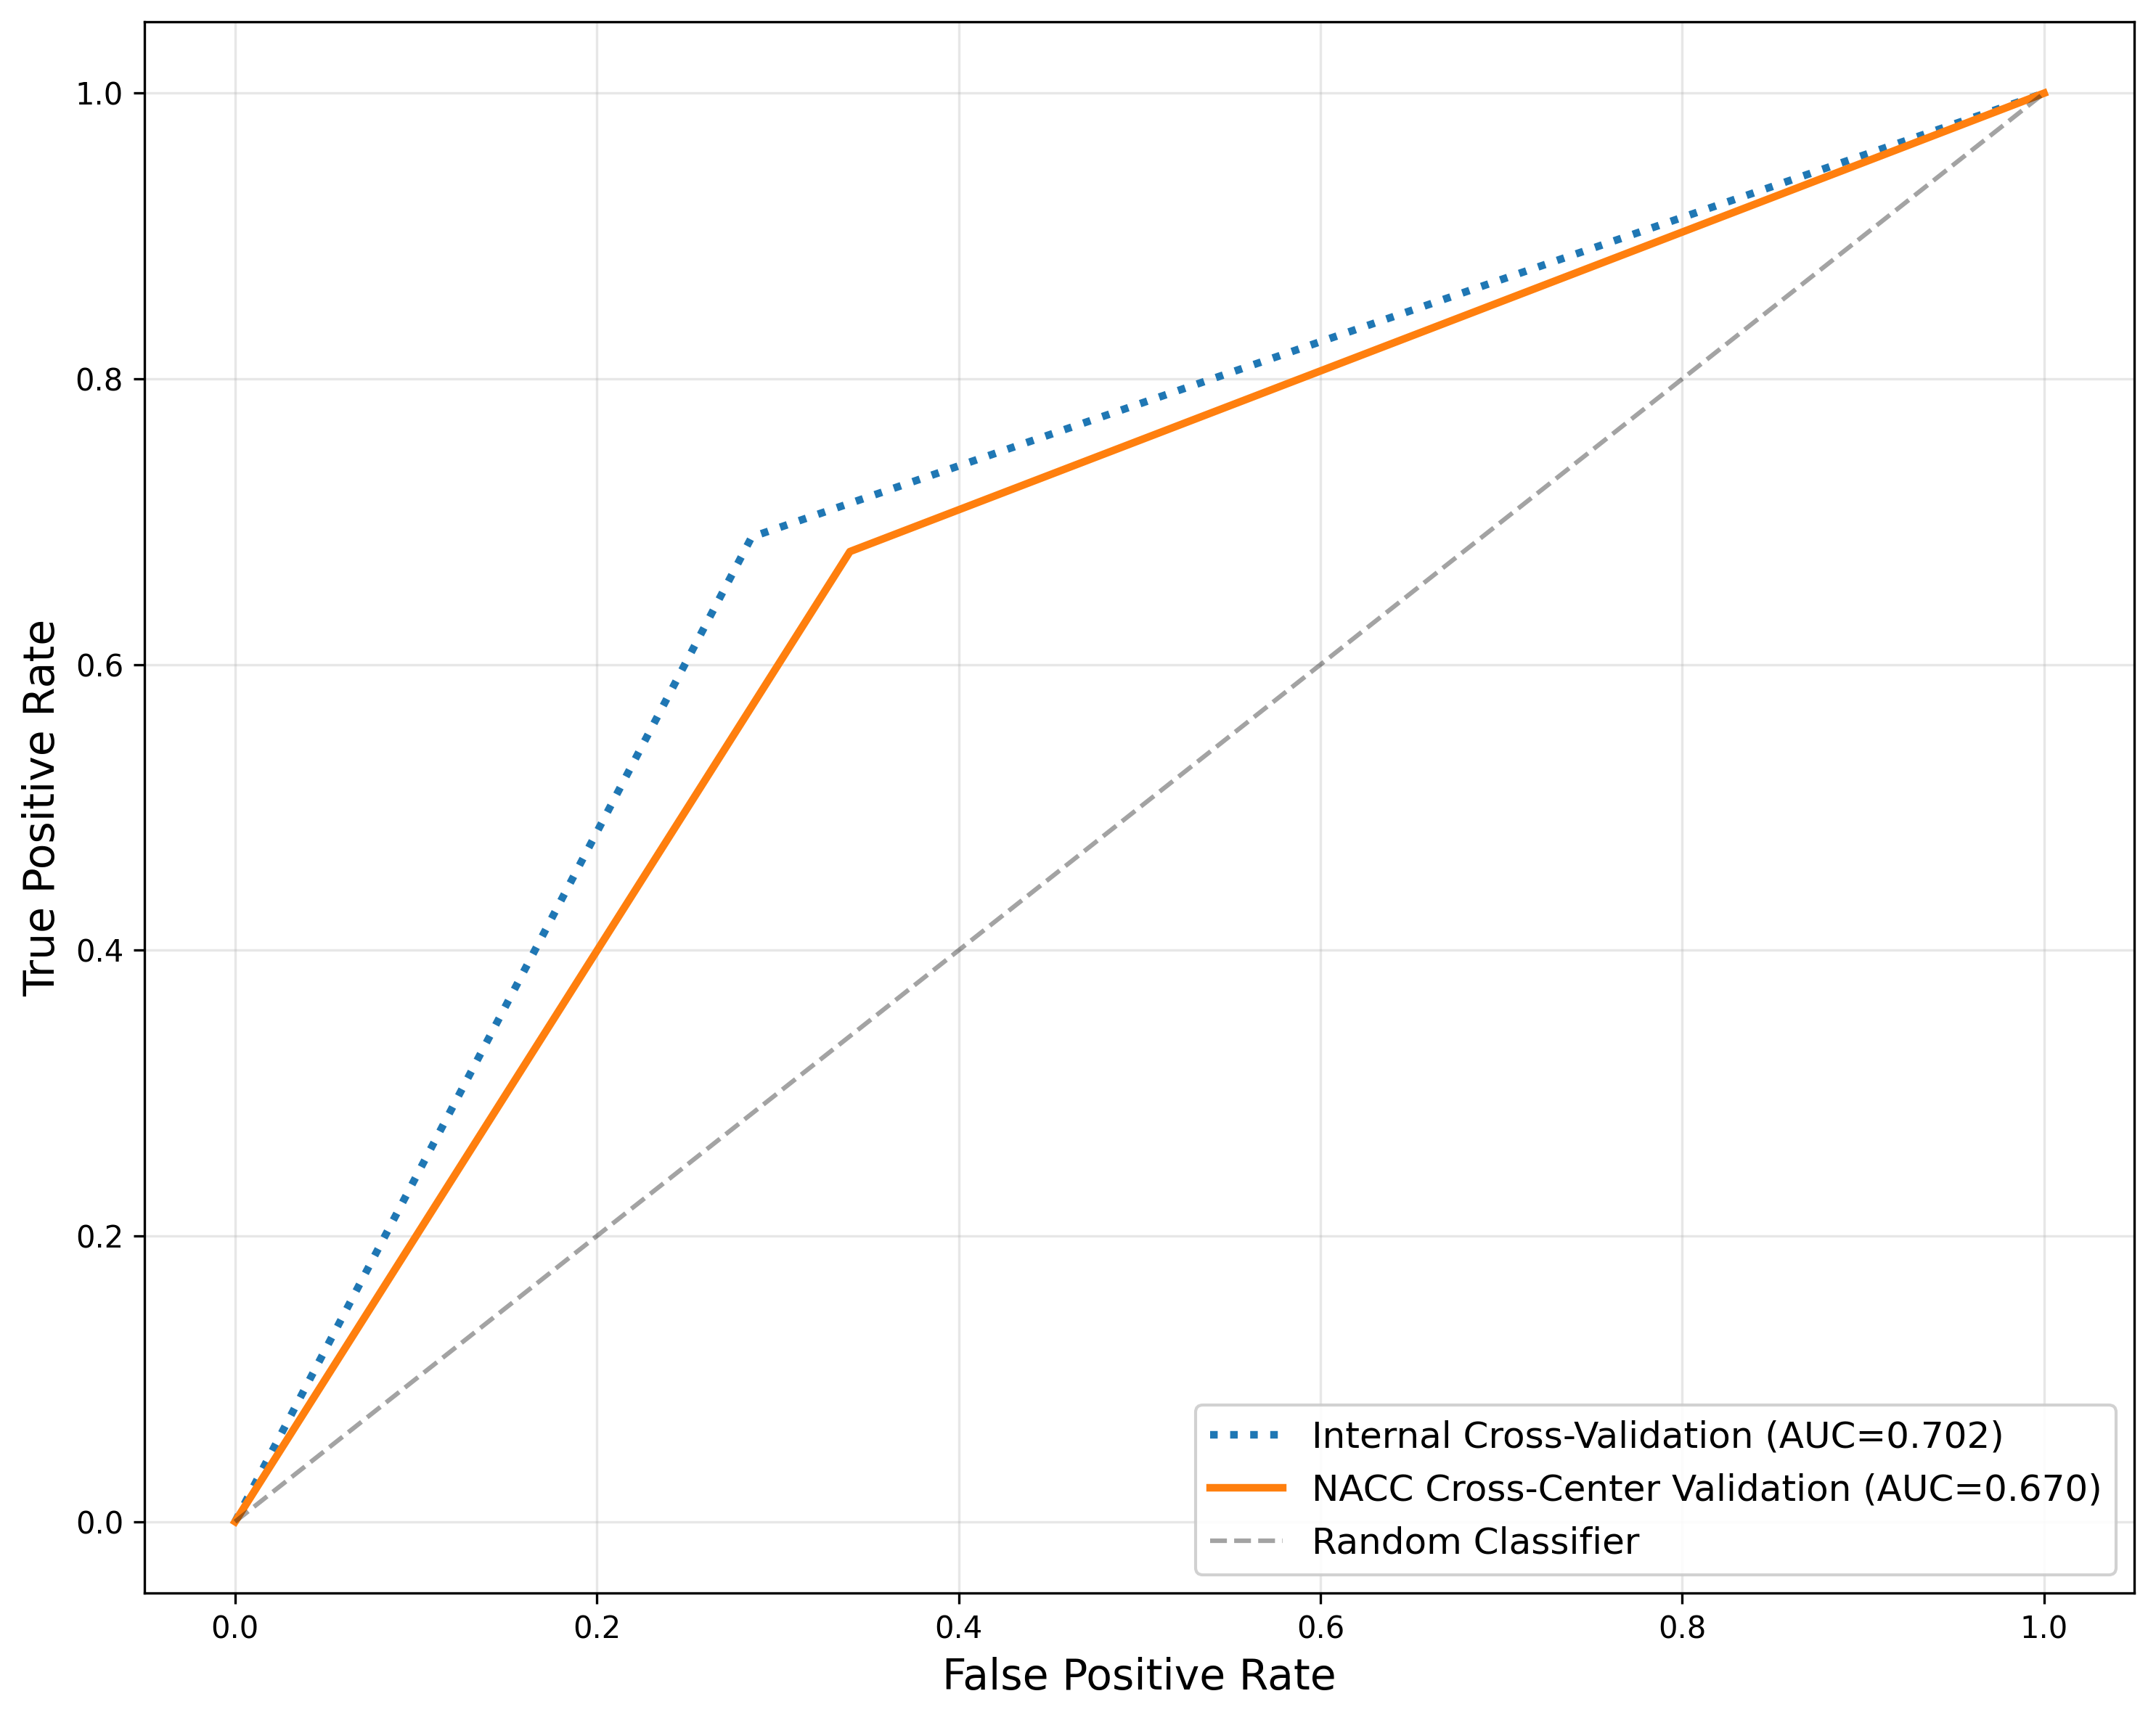
\includegraphics[width=0.7\textwidth]{figures/type_classification_all_tests_roc_overlay.png}
    \caption{ROC curves comparing the performance of the logistic regression model for the AD vs. non-AD classification task}
    \begin{minipage}{\textwidth}
      \footnotesize \hl{The horizontal axis shows the false positive rate (1 -- specificity) and the vertical axis shows the true positive rate (sensitivity). Each curve represents one validation dataset.}
    \end{minipage}
    \label{fig:ad_nonad_roc}
\end{figure}

Based on the results of the NACC cross-center validation, a moderate decrease in overall performance was observed. The AUC score decreased by 0.032, dropping from 0.702 in the internal CV to 0.670 in the NACC cross-center validation. A similar decrease was shown by the G-mean. \hl{This drop in AUC from the internal CV was statistically significant (p < 0.001), although the difference in performance is acceptable for this complex classification task.} This performance reduction confirms the high difficulty of this classification task due to the overlap in symptoms between different CI subtypes.

A slight decrease was observed in both the sensitivity and specificity scores in the unseen NACC data. The sensitivity decreased from 0.689 in the internal CV to 0.679, while the specificity decreased from 0.714 to 0.660. This indicates that the LR model found it more difficult to correctly identify cases in the NACC cross-center validation. The larger reduction in specificity means that more subjects who did not have AD were misclassified as AD. The external validation results are reported with extended performance metrics in Table~\ref{table:lr-complete-perf-task5-apdx} in the appendix.

The selected LR model was calibrated to ensure that the predicted probabilities reflect the actual risk of AD. The calibration results for NACC cross-center validation are shown in Figure~\ref{fig:ad_nonad_calib_curve}. The probabilities of the uncalibrated model were very confident in estimating extreme risk levels (slope = 0.294). However, after beta calibration was applied, the slope improved to 0.859, indicating that the model can now effectively predict AD at different probabilities thresholds. As a result, the model calibration error (ECE) decreased substantially from 0.182 to 0.042, and the Brier score improved from 0.240 to an acceptable level of 0.204, which is close to the acceptable threshold of 0.20. This highlights significant improvements in the overall alignment between the predictions and the actual observed frequencies of AD.

\begin{figure}[ht]
    \centering
    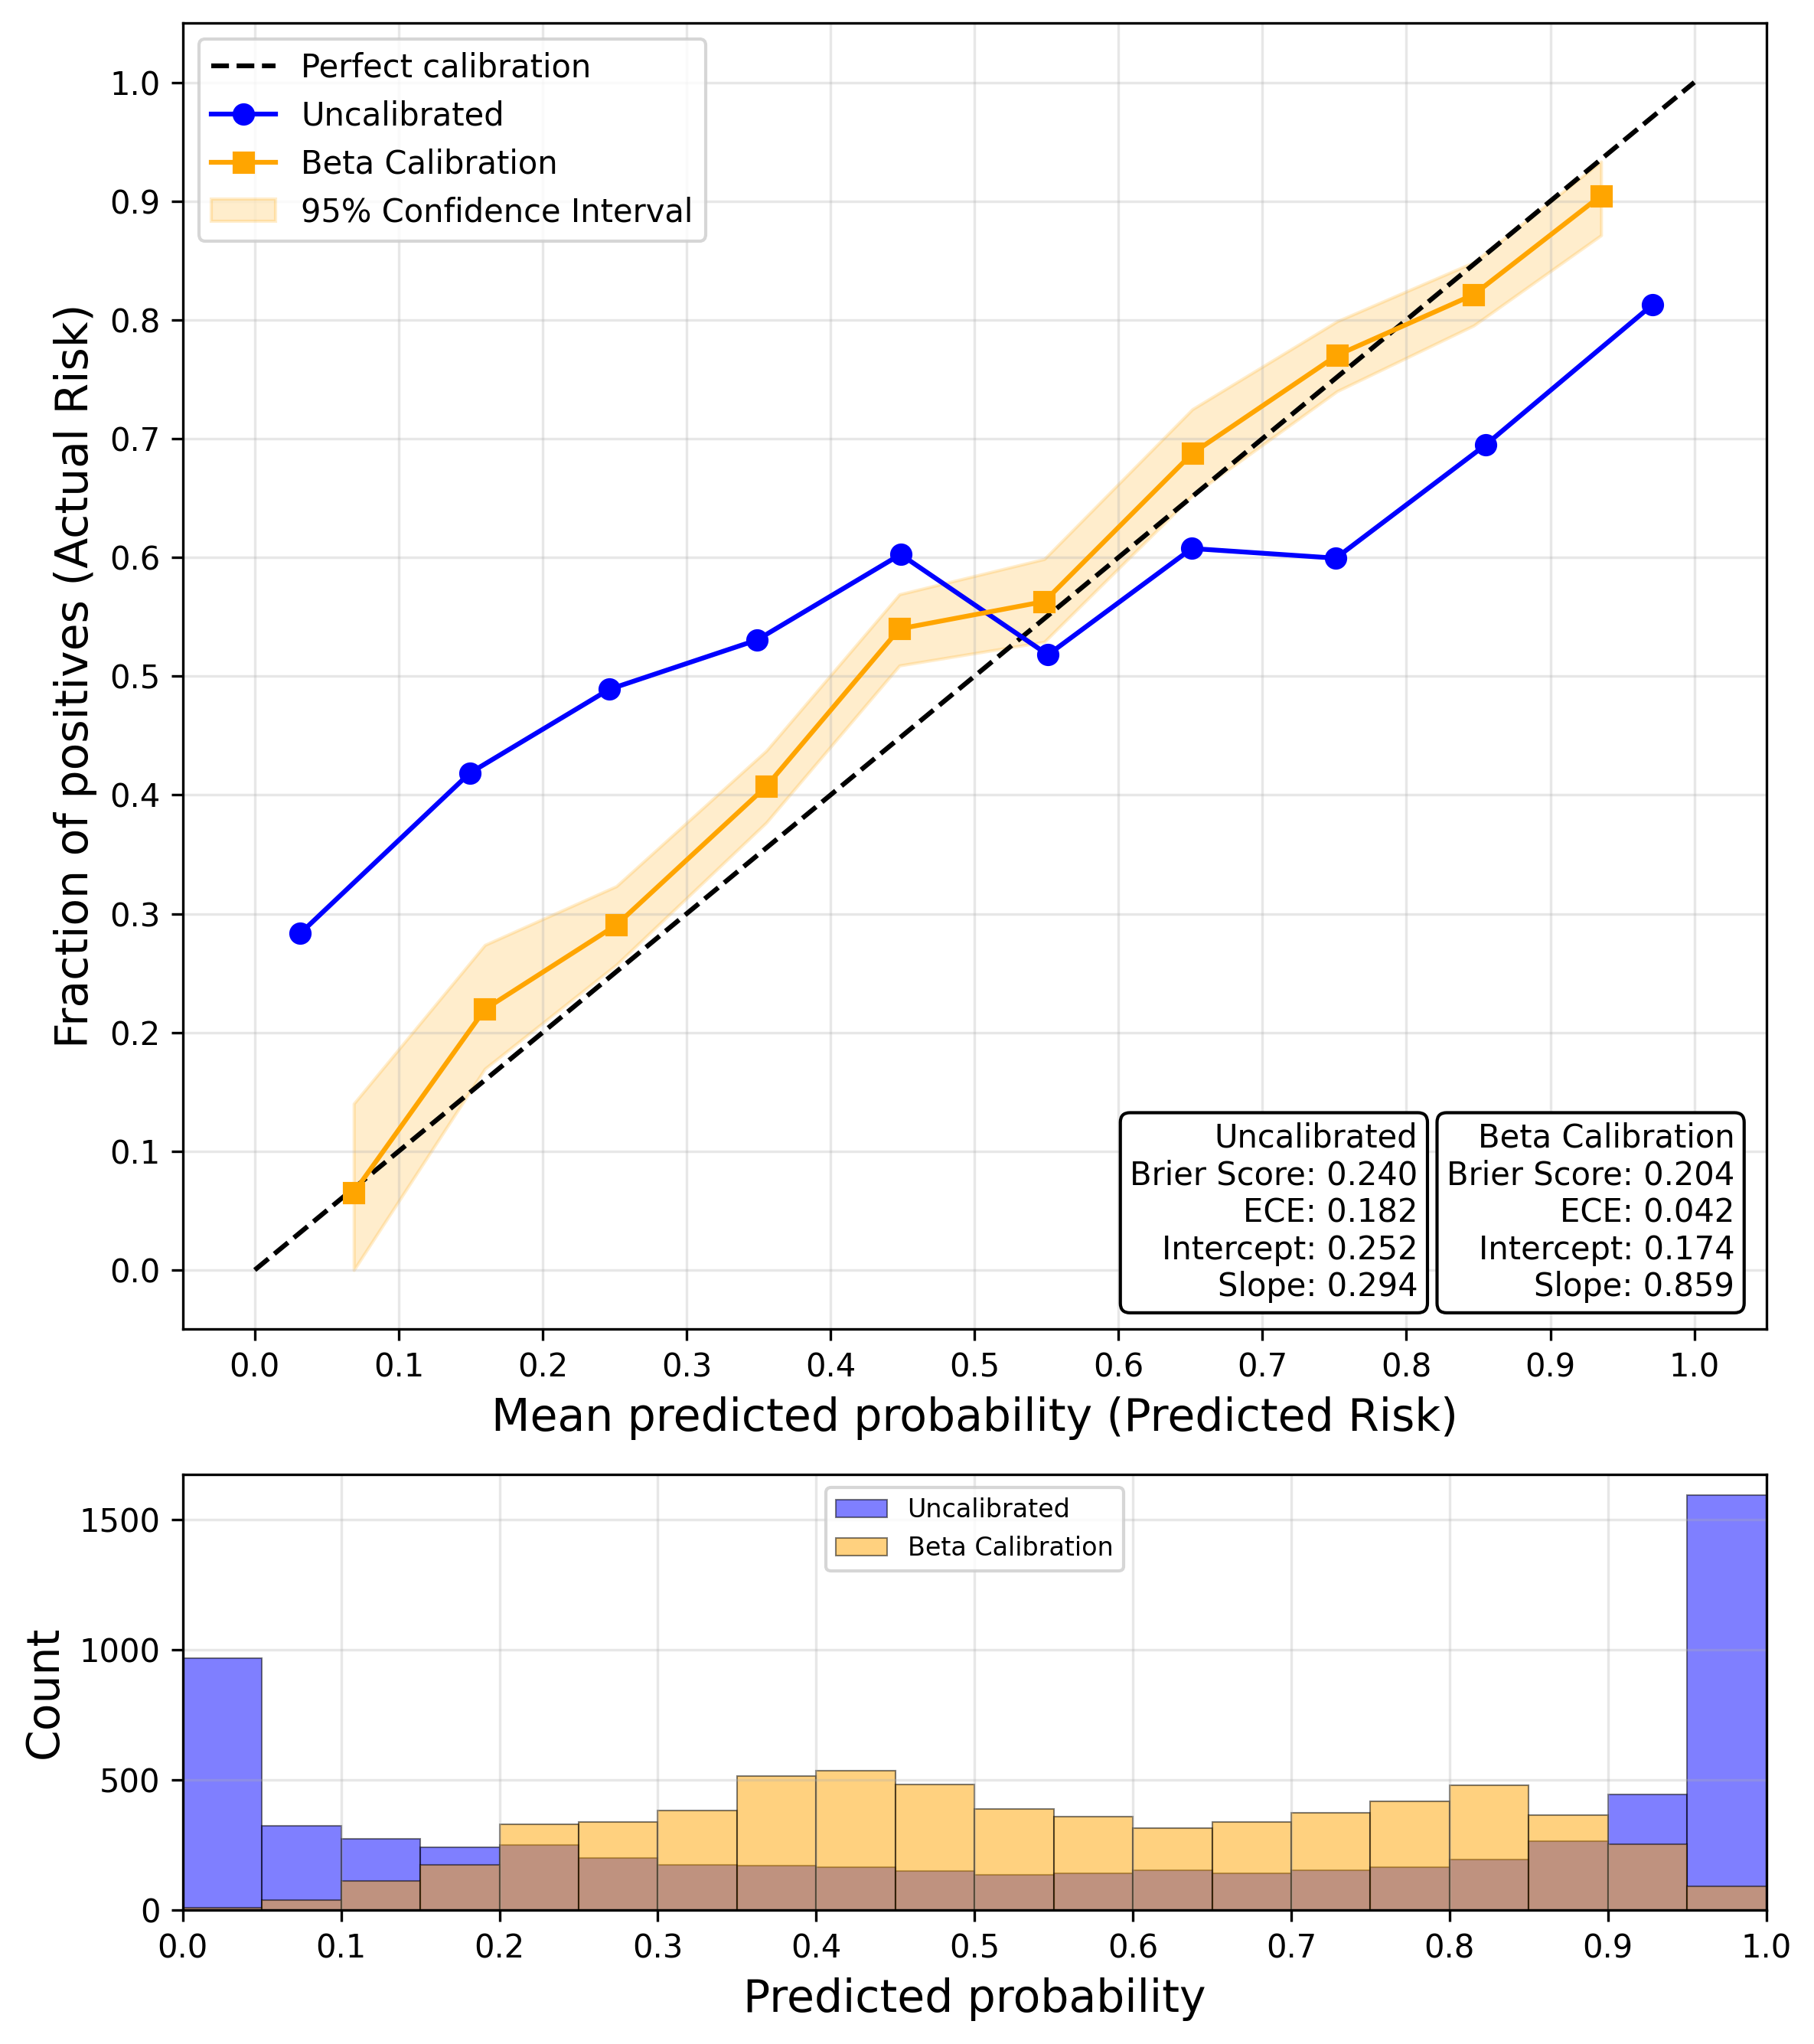
\includegraphics[width=1.0\textwidth]{figures/calibration/type_classification_nacc_test_calibration_curve.png}
    \caption{Model calibration curves of the NACC cross-center validation for the AD vs. non-AD classification task}
    \begin{minipage}{\textwidth}
      \footnotesize \hl{The horizontal axis shows the predicted probability and the vertical axis shows the observed frequency of the positive class. The diagonal line represents perfect calibration, and the curves compare the model before and after beta calibration.}
    \end{minipage}
    \label{fig:ad_nonad_calib_curve}
\end{figure}

The clinical utility of the calibrated LR model for differentiating AD from non-AD dementia was evaluated using DCA. As illustrated in Figure~\ref{fig:ad_nonad_dca}, the model presented a higher net benefit across a wide probability threshold range of 0.13 to 0.91 compared to strategies that classify all subjects as AD or all subjects as non-AD. The net benefit of the model is more pronounced in critical probability thresholds between 0.30 and 0.70. The strong clinical utility of the LR model is supported by the excellent calibration of its predicted probabilities.

\begin{figure}[ht]
    \centering
    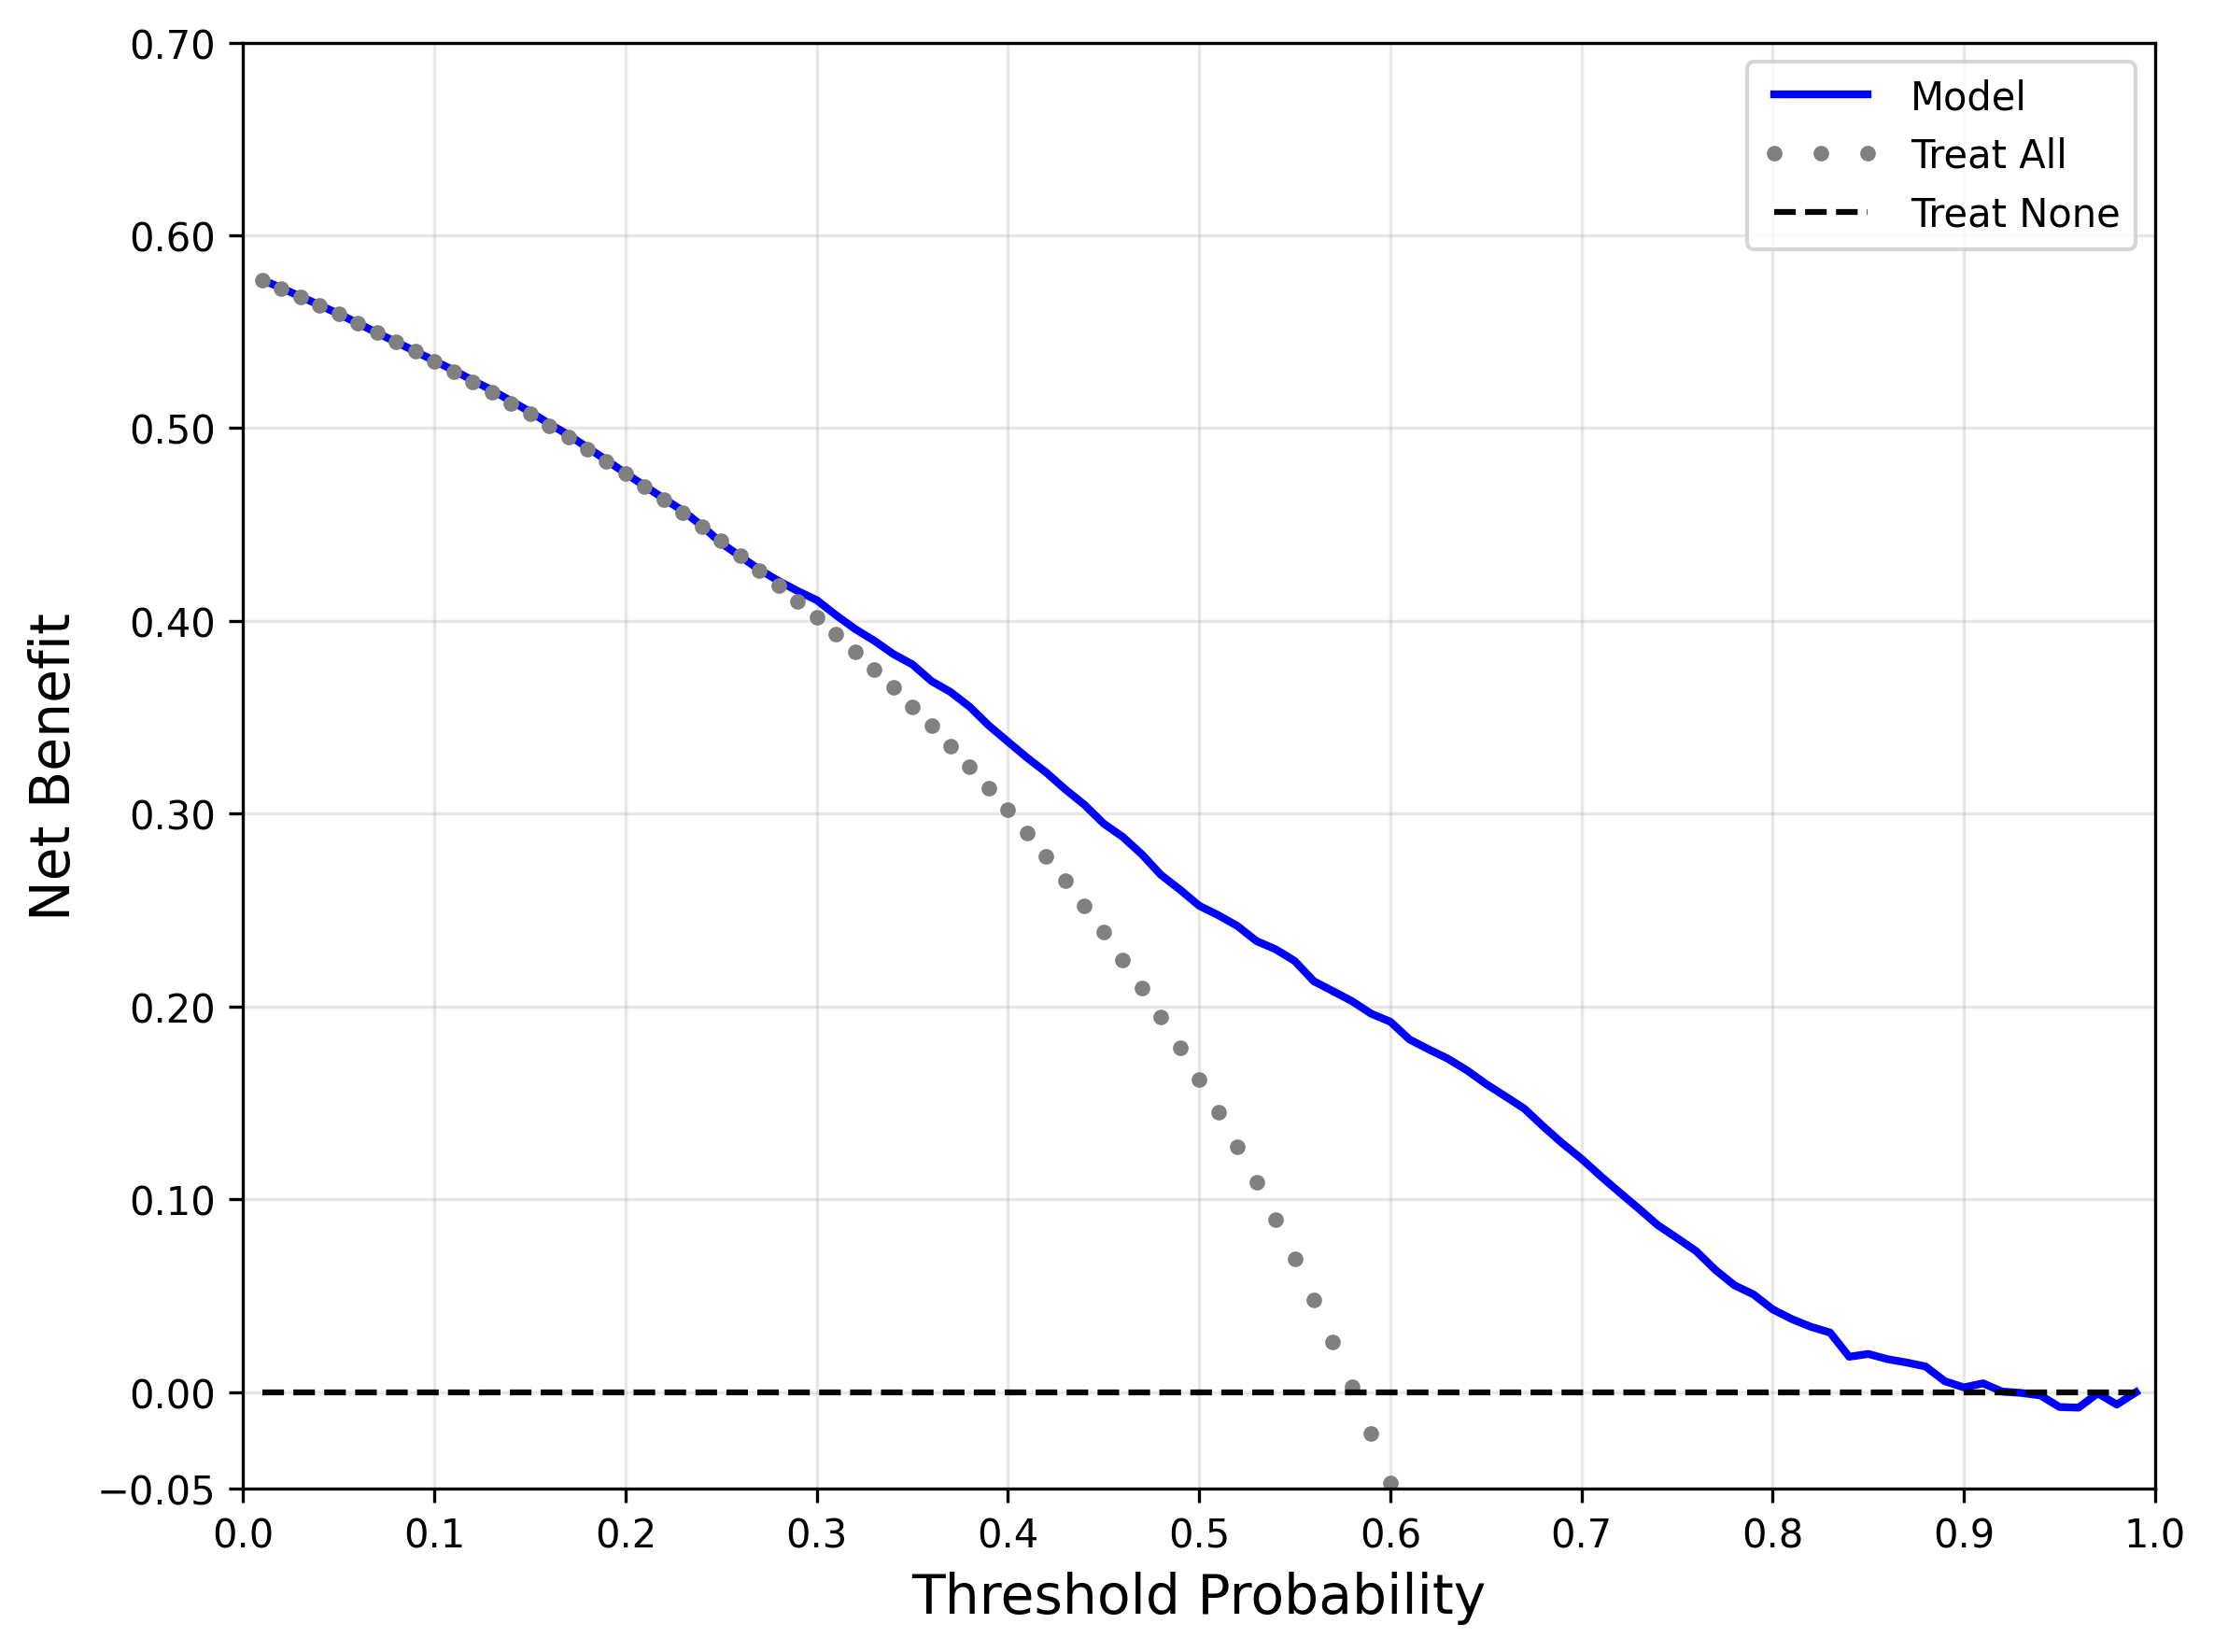
\includegraphics[width=1.0\textwidth]{figures/DCA/type_classification_dca_nacc.png}
    \caption{The decision curve analysis (DCA) of the NACC cross-center validation for the AD vs. non-AD classification task}
    \begin{minipage}{\textwidth}
      \footnotesize "Treat All" refers to the assumption that all subjects are classified as AD, and "Treat None" refers to the assumption that all subjects are classified as non-AD.
    \end{minipage}
    \label{fig:ad_nonad_dca}
\end{figure}

The results of the NACC cross-center validation showed a reasonable level of generalizability, considering the complexity of the task. Although the overall classification accuracy was slightly reduced, the selected LR model presented excellent calibration and clinical utility to classify CI subtypes. Consequently, this result supports the third research objective of developing an accessible and cost-effective model to classify CI subtypes.

\subsection{Model Explainability Results}
The bar chart in Figure~\ref{figure:ad_feature_importance} illustrates the global feature importance ranking for the classification of CI subtypes as AD or non-AD. As expected, the LR model was largely influenced by the features obtained from CDR. Memory impairment (MEMORY) was identified as the most important feature, having a SHAP value that significantly exceeds most of the other features. It was observed that moderate and severe memory impairment mainly associated with AD diagnosis. A similar importance pattern was observed with the impairments in orientation (ORIENT), which was ranked as the second most important feature. It was followed by challenges related to personal care (PERSCARE), but impairments in this domain contributed to the classification of non-AD. Demographic influence was also observed, with age (NACCAGE) ranking as the fourth most critical factor. Older subjects were found to be more likely to be classified as AD. Interestingly, the functional ability to remember dates (REMDATES) played a minimal role in this task, ranking as the second least important feature despite being a top predictor for classifying cognitive decline in the other classification tasks. This indicates that while functional assessments are excellent for classifying cognitive status, clinical ratings (CDR) are more effective for determining the specific etiology (AD vs. non-AD).

\begin{figure}[ht]
    \centering
    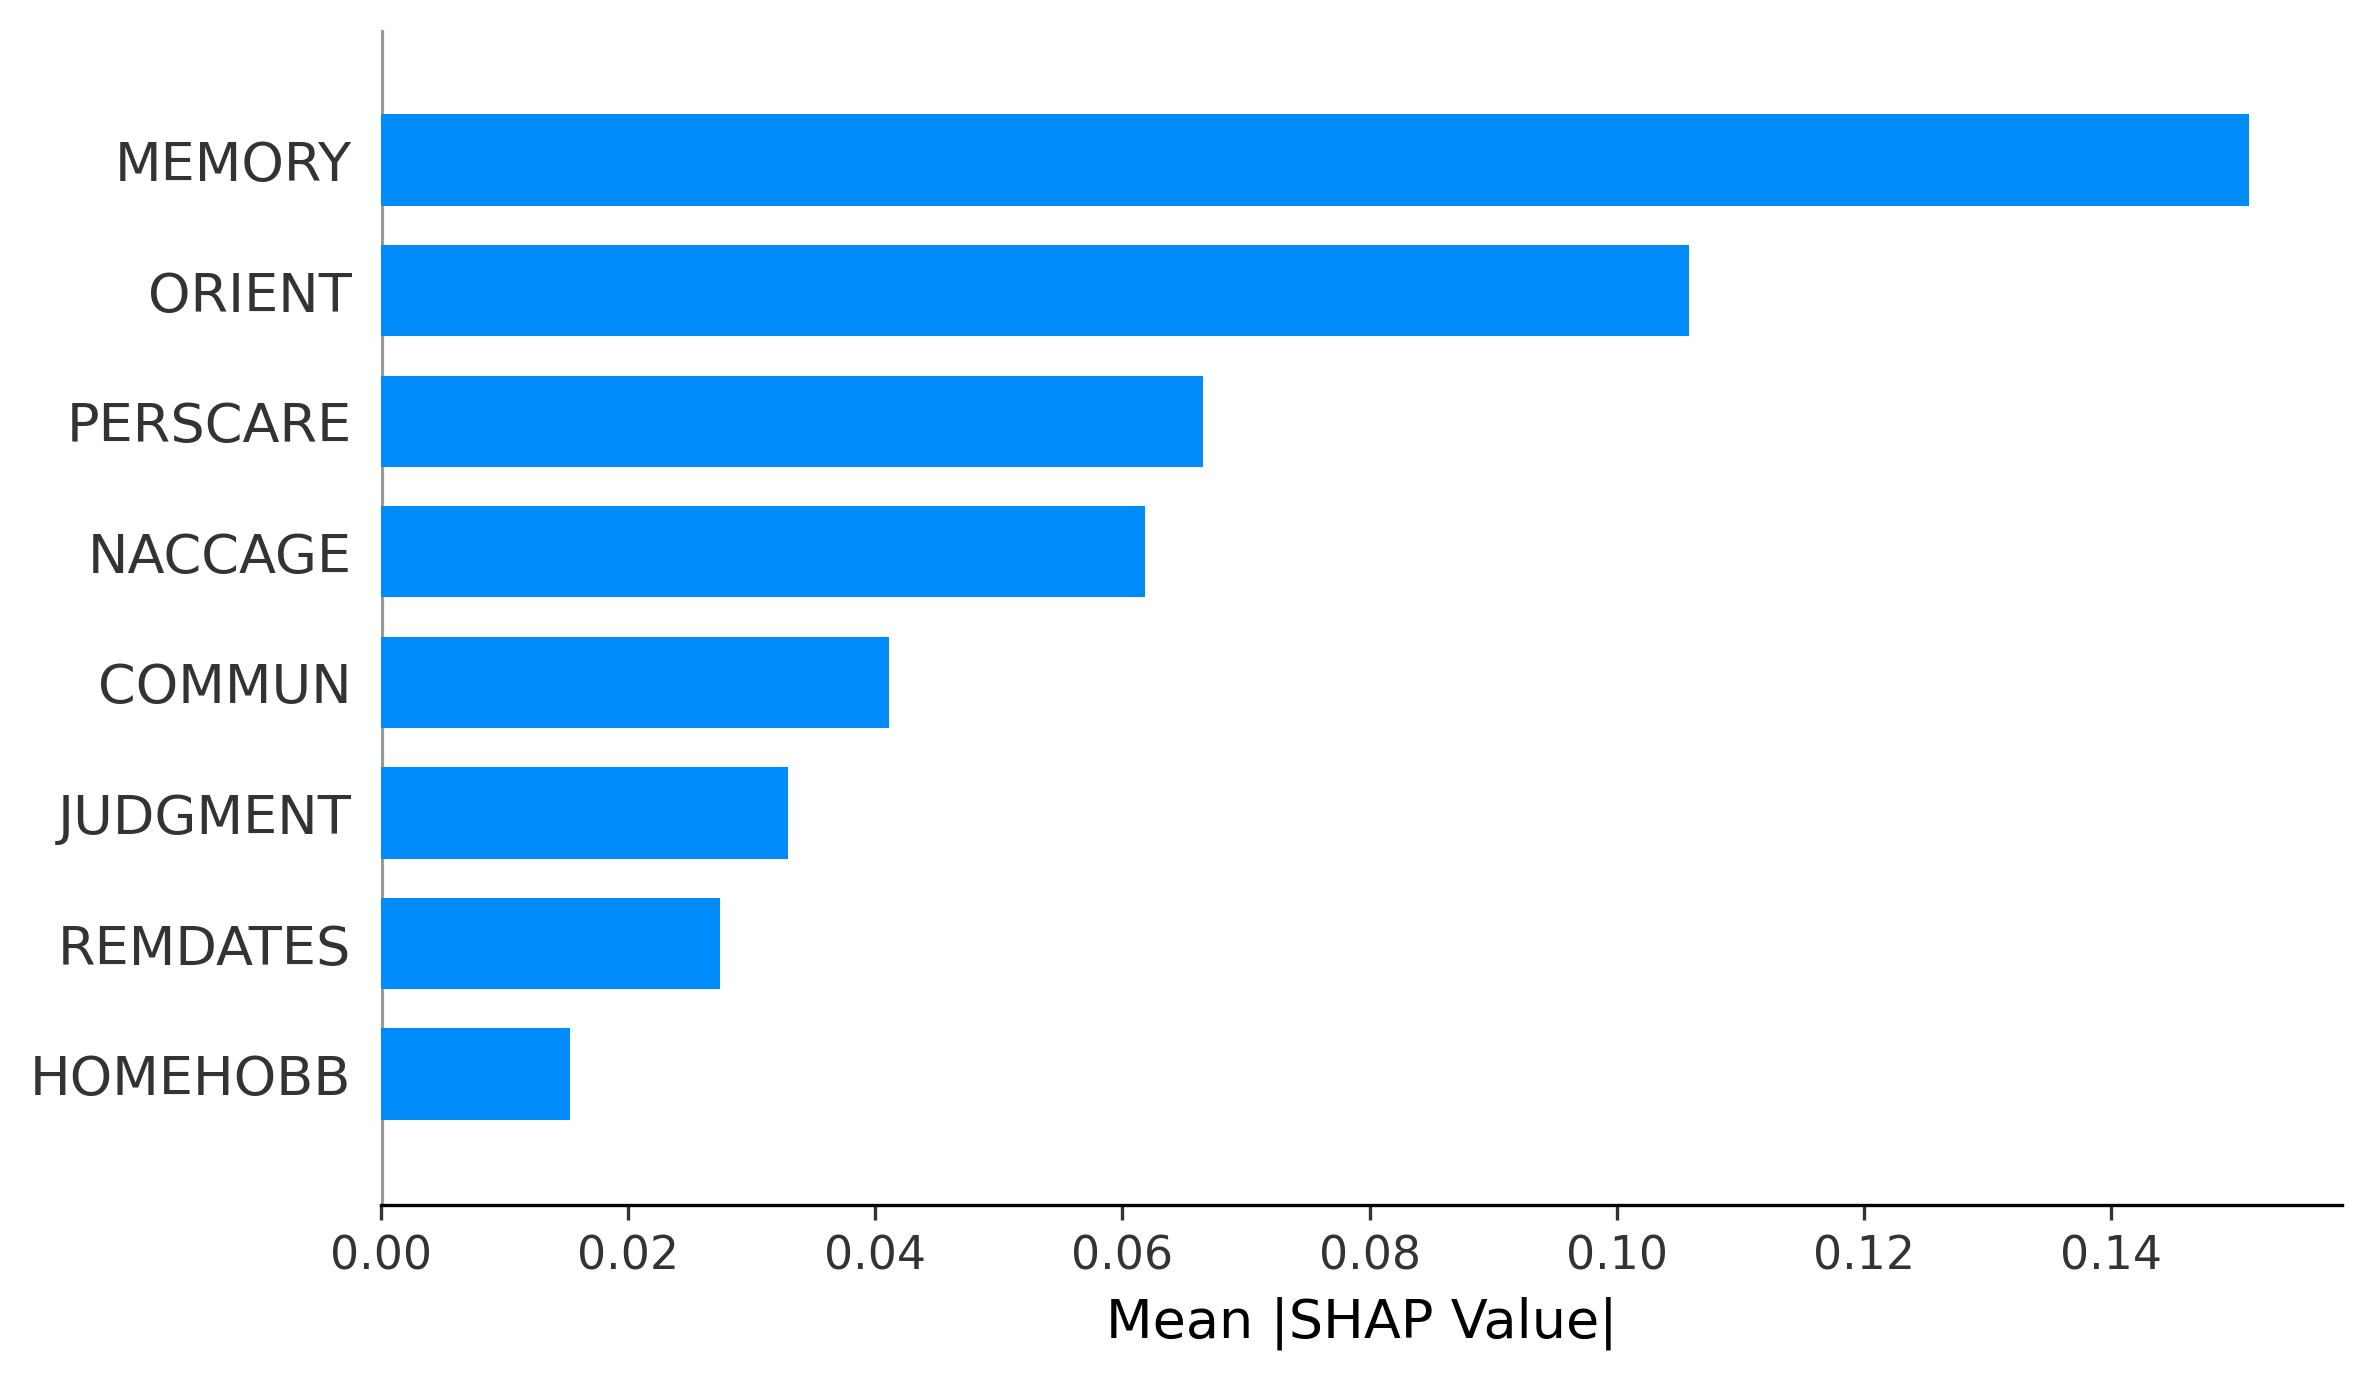
\includegraphics[width=1.0\textwidth]{figures/XAI/type_classification_nacc_shap_barchart.png}
    \caption{Feature importance in the NACC cross-center validation and the ADNI external validation for the AD vs. non-AD classification task}
    \begin{minipage}{\textwidth}
      \footnotesize \hl{The bars represent the mean absolute SHAP value of each feature, which ranks the contribution of the feature to the model prediction in the two validation datasets.}
    \end{minipage}
    \label{figure:ad_feature_importance}
\end{figure}

In this task, a local explanation was performed to evaluate how the features contribute to the model classification at the individual levels. Two correctly classified AD instances were randomly selected for analysis. The influence of features in these two instances is presented by SHAP waterfall plots in Figure~\ref{figure:ad_pos_waterfall}. The instances have different feature values that led to the classification of AD, although both resulted in a probability of 53\%. In Instance B, AD classification was primarily driven by mild impairments in orientation (ORIENT) and memory (MEMORY). In contrast, Instance A's older age combined with preserved ability of personal care (PERSCARE) was sufficient to push the classification towards AD despite questionable impairment in memory.

\begin{figure}[ht]
    \centering
    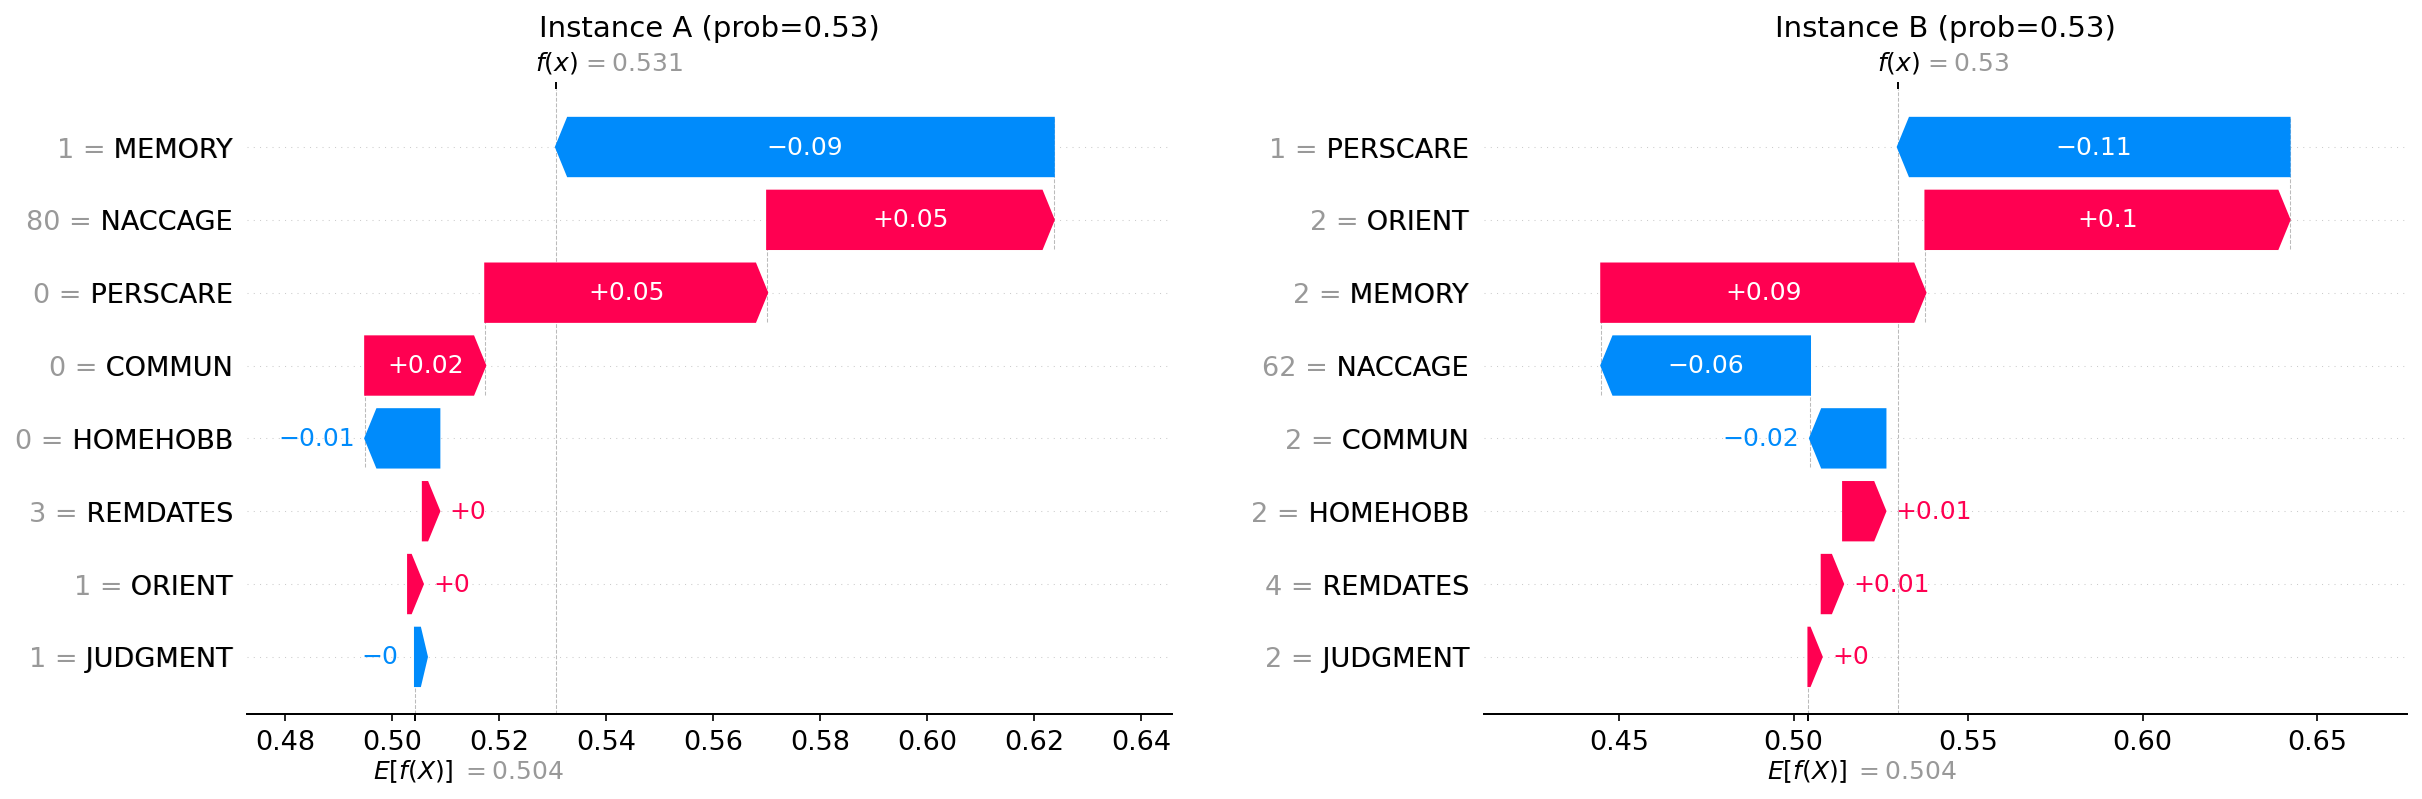
\includegraphics[width=1.0\textwidth]{figures/XAI/type_classification_nacc_true_positive_waterfall.png}
    \caption{SHAP waterfall plots for two instances correctly classified as Alzheimer's disease}
    \begin{minipage}{\textwidth}
      \footnotesize \hl{The plot shows how the value of each feature shifts the prediction from the base value to the final predicted probability for a single instance.}
    \end{minipage}
    \label{figure:ad_pos_waterfall}
\end{figure}

\newpage
A similar analysis was performed with two non-AD instances in Figure~\ref{figure:ad_neg_waterfall}. \textit{Instance A} represents a scenario where the AD indicator of 86 years of age was successfully reversed by preserving key cognitive functions, specifically normal orientation and only questionable memory impairment. \textit{Instance B} presented a different profile. It was classified as non-AD regardless of mild memory impairment. This is due to the questionable ability of personal care despite a relatively younger age. As a side note, it can be observed that features with low global importance have minimal to no influence on the model outcome in the four individually explained instances.

\begin{figure}[ht]
    \centering
    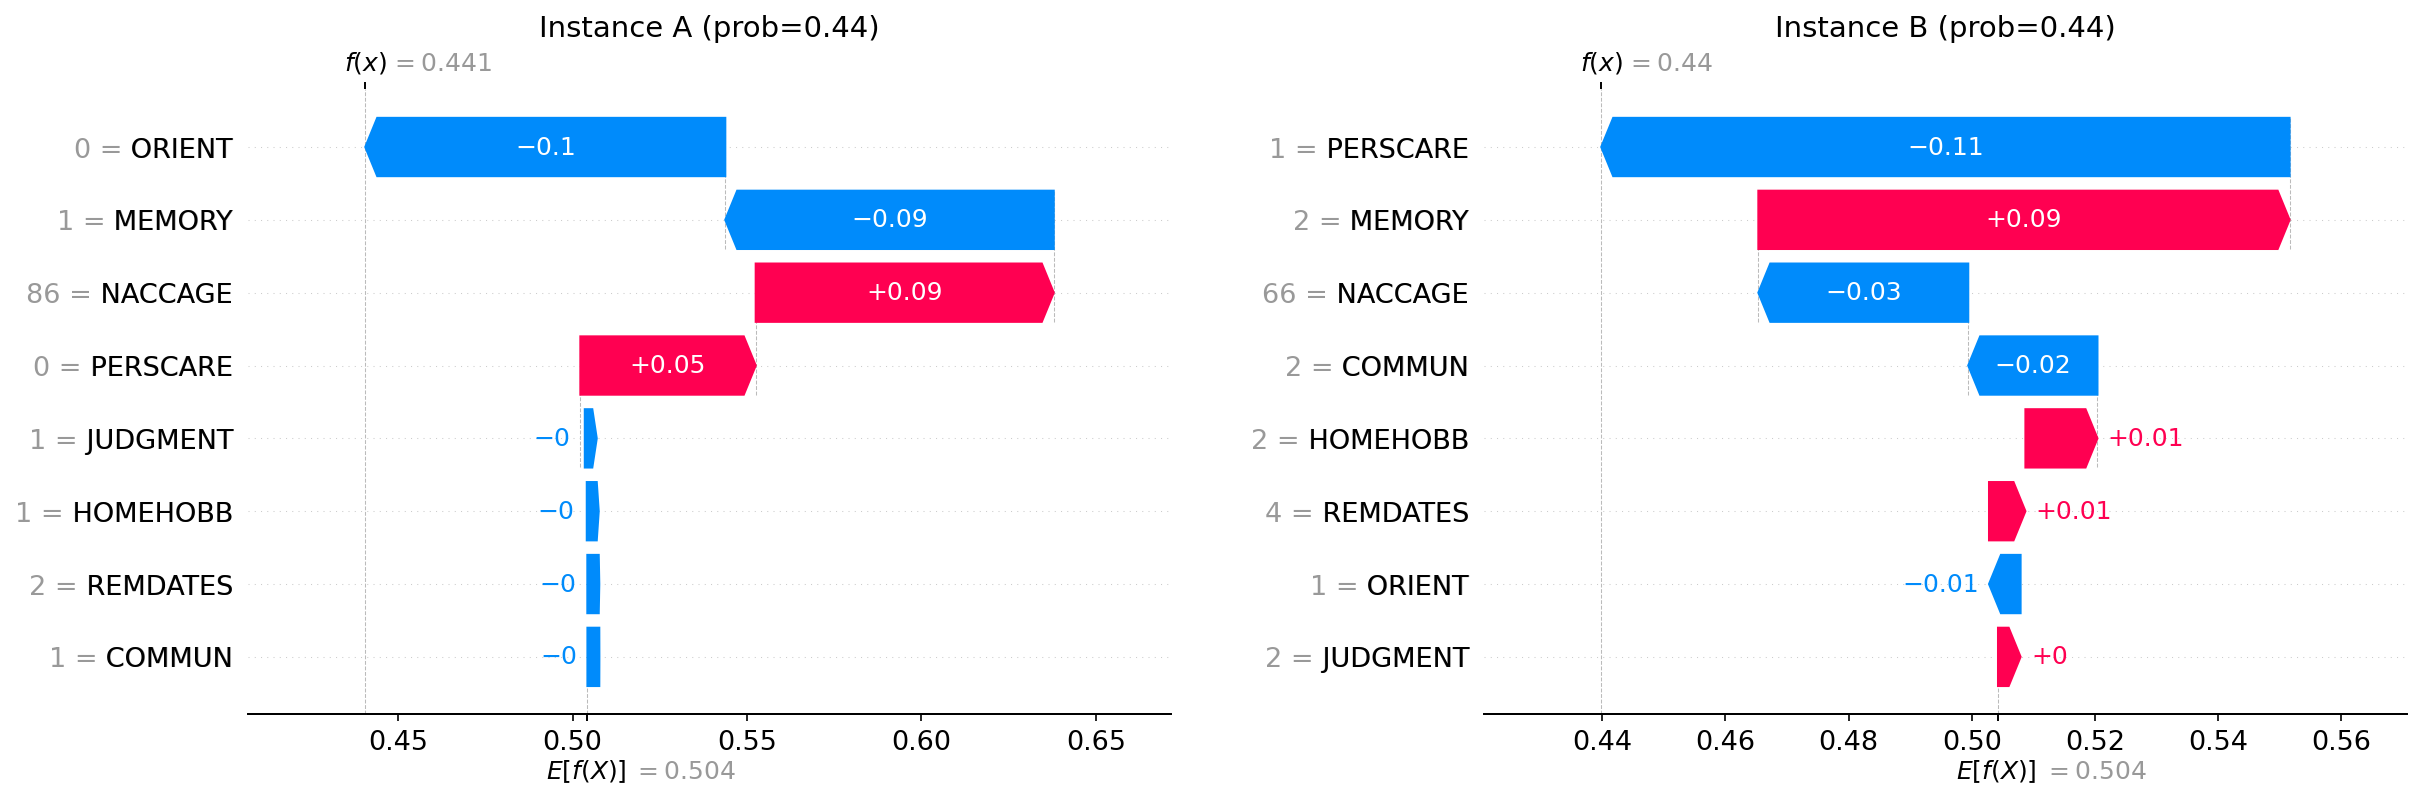
\includegraphics[width=1.0\textwidth]{figures/XAI/type_classification_nacc_true_negative_waterfall.png}
    \caption{SHAP waterfall plots for two instances correctly classified as non Alzheimer's disease}
    \begin{minipage}{\textwidth}
      \footnotesize \hl{The plot shows how the value of each feature shifts the prediction from the base value to the final predicted probability for a single instance.}
    \end{minipage}
    \label{figure:ad_neg_waterfall}
\end{figure} % Results and Analysis
% !TEX ROOT = thesis.tex
\chapter{Discussion}

\hspace{12.7mm}This chapter interprets and analyzes the research findings. It also provides a detailed discussion of the implications of the obtained results and the significance of the study. In addition, a comparison with the existing literature is included to highlight the contribution of this study to the field. The chapter is organized in multiple sections to discuss the results of the key methods in this research. 

\section{Automatic Ensemble Feature Selection}
The proposed automatic ensemble feature selection method was successful in its main goal. It consistently identified minimal and computationally efficient feature subsets for all five classification tasks. This is a key step for developing cost-effective models, which is a main objective of this research. This was achieved through the method's novel design, which works to find the number of features where adding more features provides a diminishing reduction in class overlap. This process ensures a balance between model simplicity and class separability. As a result, the method selected the smallest and most informative feature set. For instance, it reduced the feature count by around 82\% (from 68 to 12) for the normal cognition (\acrshort{NC}) vs. cognitive impairment (\acrshort{CI}) task and by approximately 85\% (from 71 to 11) for the cognitive impairment but not dementia (\acrshort{CIND}) vs. dementia task. This large reduction in features directly improved computational efficiency, making model training over 2.7 times faster than the baseline in both tasks. 

An important finding was related to the class overlap. The proposed method is designed to always select feature sets with the lowest F1 feature overlap scores. However, this reduction in class overlap did not directly result in the best predictive performance for all models. This was most clear in the future prediction tasks and the CI subtype classification task. In these tasks, the feature sets with the lowest class overlap produced a lower geometric mean (\acrshort{G-mean}) score with the random forest (\acrshort{RF}) model compared to the baseline and the Boruta method. This finding suggests a model-dependent effect. The F1 is a measure of linear separability based on Fisher's Discriminant Ratio. As a result, the method selected features that were highly effective for linear classifiers like logistic regression (\acrshort{LR}). In fact, for LR models, the minimal set selected by the proposed method performed equal to or better than the feature set selected by the Boruta method. 

In contrast, the non-linear RF model may have benefited from the larger, more complex feature sets of the baseline. Additionally, the Boruta method is a wrapper feature selection method based on an RF model. Therefore, it selects features that are optimized for an RF classifier. Because both the selection algorithm and the evaluation model are based on RF, it is logical that this method would produce a feature set that performs well for this specific model. On the other hand, the proposed method is model agnostic and optimized for a linear separability measure, which explains why it showed highly competitive performance with a linear model like LR. Therefore, the use of the proposed method aligns with the objective of this study since it contributes to improving the performance of linear models, which are generally more efficient and interpretable compared to non-linear models. 

Looking at the types of the selected features in different classification tasks, the analysis indicates a very strong and consistent pattern. For all four cognitive status classification and prediction tasks, the most dominant group of selected features was from the assessments of instrumental activities of daily living (\acrshort{IADL}) from the Functional Activities Questionnaire (\acrshort{FAQ}). This finding is logical. It aligns with the clinical definition of CI, which is primarily characterized by a decline in a person's ability to perform daily functional activities. In addition, similar studies in the literature also reported that IADL assessments are one of the top predictors of CI and dementia \cite{abbas2024Explainable, Ren2023Improving, Richter2025Cognitive}. \hl{This was also observed in prediction models from different countries, including LMICs} \cite{Cui2024Prediction, Ren2025Using}. Table~\ref{table:feature-details} in the appendix provides details about the selected features in all classification tasks.

A closer look at the IADL assessments shows that a constant set of features, such as BILLS, TAXES, SHOPPING, REMDATES, and TRAVEL, were selected in all four status tasks. \hl{The diagnostic value of these features is also supported by clinical evidence} \cite{Teng2010Utility}. Moreover, these functional features were consistently selected along with basic demographics (such as NACCAGE) and subjective memory complaint (MEMPROB). This finding has a high practical value. It suggests that in clinical practice, only a small set of data needs to be collected from the patient to run all the different models and provide a complete CI risk assessment. This makes the entire assessment workflow more cost-effective for application in clinical practice by reducing the cost and time required to gather the required data. 

For the more complex classification task of the CI subtypes (Alzheimer's disease (\acrshort{AD}) vs. non-AD), the feature set was dominated by the Clinical Dementia Rating (\acrshort{CDR}) scores, since all six CDR features were selected. The CDR scale is able to assess the nature and severity of the impairment in multiple cognitive domains. This finding indicates that the inclusion of CDR features is important to differentiate between AD and non-AD disorders as these classes cannot be effectively classified using demographic and functional assessment data. Similar studies also used CDR scores to differentiate AD from mild cognitive impairment \cite{abbas2024Explainable, Pang2023Predicting}. 

In summary, the proposed method successfully achieved its main goal of identifying effective and computationally efficient feature sets for all tasks. A key finding was that the method's model-agnostic design makes it particularly effective for linear models, which aligns with the research objective of developing cost-effective and interpretable models.

\section{Data Resampling}
The data complexity was analyzed in each of the tasks in this study to apply proper data resampling methods that could boost the performance of the machine learning models. The class imbalance ratio (\acrshort{IR}) was found to be relatively low in all tasks, ranging from 1.18 to 1.46. In contrast, class overlap was consistently high in the majority of tasks. The class instances were mostly overlapped at the global structural level, with the \acrshort{N1} scores ranging from approximately 0.30 in the current classification tasks to extreme values exceeding 0.50 in the CI subtype classification tasks. This suggests that utilizing only accessible data to predict cognitive impairment could result in structural intertwining of the classes in the feature space even if the class imbalance is minor. With demographic, depression scale, and cognitive assessment data, it is challenging to determine what cognitive status a subject might have in the future or to classify their CI subtypes as AD or non-AD. This is because many cases share similar values in these low discriminative data domains.

A comprehensive interpretation of various data resampling methods highlights the importance of handling class overlap, instead of only handling class imbalance, to obtain better classification performance using accessible data. In the NC vs. CI classification task, the baseline model struggled more in accurately classifying the majority class (CI) than the minority class (NC). This behavior indicates that due to the moderate class overlap, the model could not learn a distinct pattern of CI, even though there were more instances of CI than NC. As a result, despite how skewed the classes are, handling class overlap is necessary to obtain reasonable accuracy for both classes. Compared with other data resampling methods, the proposed method made the feature space easier to separate by removing noisy, confusing instances and strengthening the representation of the minority class in safe areas. This made the classes more distinct, resulting in slightly better recall in both classes.

The class overlap-guided data resampling method resulted in even better performance improvement in the future cognitive status prediction tasks. In these tasks, classes are highly intertwined because accessible data have limited discriminative power of future cognitive status. The proposed method employed the Edited Nearest Neighbor (\acrshort{ENN}) method, which analyzes the neighbors of all instances of both classes and removes instances surrounded by neighbors of the opposing class. After that, a suitable targeted oversampling method was applied to populate the sparse regions of the minority class. This process restructured the training data by eliminating confusing instances with similar feature values and systematically generating new instances that enhanced the definition of the decision boundaries. Consequently, the performance of the RF model improved significantly, especially in the future CIND vs. dementia prediction task, resulting in the best recall in both classes.

An opposite of class overlap guided data resampling is random resampling and Synthetic Minority Over-sampling Technique (\acrshort{SMOTE}). These standard techniques proved their ineffectiveness in the future cognitive status prediction tasks. For instance, Random Oversampling (\acrshort{ROS}) and SMOTE generated new instances in ways that worsened or did not resolve the class overlap (SMOTE increased the N1 score in the future NC vs. CI prediction task). ROS randomly duplicates minority class instances, including those in overlapped regions, whereas SMOTE creates synthetic instances by interpolating points within the complex boundary regions. Such oversampling approaches improved the RF model's recall of the minority class but considerably reduced its ability to correctly identify the majority class.

The Random Undersampling (\acrshort{RUS}) method also demonstrated similar deficiencies. While RUS could remove overlapped instances of the majority class, it could also remove informative instances in safe data regions, resulting in more complex data. For instance, RUS resulted in the worst dementia prediction accuracy of 0.723 compared to 0.77 of the baseline and 0.776 of the proposed method. This trade-off could be undesirable in certain real-world clinical scenarios, as it increases the risk of missing actual dementia cases.

By analyzing the relationship between class overlap measures and the improvement in the RF performance, it can be realized that handling class overlap is particularly valuable in classification problems characterized by high structural complexity. This relation was mainly observed in the AD vs. non-AD classification task, which presented the highest degree of structural class overlap. In this task, the proposed method achieved the highest recall for both the AD and non-AD classes simultaneously.

\newpage
Data cleaning by ENN is a major factor in the success of the proposed method. While ENN helped the model focus on clear patterns by eliminating confusing and probably noisy instances, it could have possibly removed informative instances that represent valid characteristics of both classes. However, in general, this method showed potential in improving the quality of the training data of the National Alzheimer's Coordinating Center (\acrshort{NACC}) Uniform Data Set (\acrshort{UDS}), where subjects might have been misdiagnosed or experienced fluctuating cognitive status.

It is important to note that in certain tasks, such as the prediction of future NC vs. CI, the overall improvement in the G-mean was marginal, even though the class overlap was successfully resolved. This slight increase could be due to the inherent informational limitation of the data used in this study. Although the proposed method maximized the learnability of the data by minimizing class overlap, it was unable to generate information that was absent from the feature set. Further enhancement of the model's accuracy in predicting future cognitive status or classifying CI subtype might require more data that bring fresh and different information beyond demographics and basic cognitive assessments.

In summary, the results demonstrated that poor performance attributed to low-cost, accessible data is largely due to structural class overlap. It is possible to resolve this overlap and produce accurate and clinically viable predictive models of CI without the use of expensive biomarkers by applying the designed data resampling method. This supports the research objective of developing accessible CI screening models in resource-constrained settings.

\section{Model Fine-Tuning and Selection}

Following the data preprocessing phase, five different machine learning algorithms were optimized to select the best set of hyperparameters that can provide a balance between predictive accuracy and computational efficiency. The selection was automated using the novel cost-effective model selection algorithm (Algorithm \ref{alg:model-selection}). This section discusses the key findings of this process.

\subsection{Efficacy of the Cost-Effective Model Selection Algorithm}
The application of the proposed selection algorithm resulted in significant improvements in computational efficiency across various models. The algorithm allowed for the selection of cost-effective models, which increased the prediction speed without causing a statistically significant decrease in classification performance. For instance, in the future CIND vs. dementia prediction task, the prediction throughput of the selected cost-effective k-Nearest Neighbors (\acrshort{KNN}) model was increased by 3.15 compared to a model with the best performance. Similarly, in the future NC vs. CI prediction task, the training speed of the Light Gradient Boosting Machine (\acrshort{LightGBM}) model was improved by 3.59 times. These gains were achieved while keeping the performance reduction strictly within 1\% of the best obtained performance. Section~\ref{sec:lr-fine-tuning-apdx} in the appendix demonstrates how the proposed model selection algorithm was able to select the most cost-effective LR models in all classification tasks.

These results suggest that the benchmark models, which were identified by the algorithm based on the best classification accuracy, were often over-parameterized. The selection algorithm successfully selected hyperparameters that are able to learn the essential patterns in the training data without unnecessary computational complexity. For instance, the selection algorithm continuously selected shallower trees for ensemble models and simplified distance metrics for KNN models.

Beyond the scope of this study, the proposed cost-effective model selection algorithm offers more valuable advantages in terms of its practical use. The structured three-phase approach of the algorithm streamlines and automates the complexity of the model selection process and promotes model selection criteria beyond classification performance. This structured design allows technical and non-technical users to easily understand how the algorithm works and produce the intended output. Moreover, the algorithm is designed with multiple parameters to define different performance and efficiency requirements. This indicates that the algorithm is highly adaptable to various industrial and academic applications. Furthermore, the algorithm can be easily integrated into existing machine learning pipelines, which strengthens its practical utility. Section~\ref{sec:selection-algorithm-usecases-apdx} in the appendix discusses how the proposed cost-effective model selection algorithm can be utilized in various use cases.

\subsection{Final Model Selection}
Based on the comparative analysis, LR was selected as the final model for all classification tasks in this study. It was observed that the LR model achieved performance that was statistically comparable to complex non-linear models, such as RF, LightGBM, and Support Vector Machines (\acrshort{SVM}). For instance, in the NC vs. CI classification task, the LR model achieved an F1-score of 0.848, which was very close to that of the RF model (0.849) and better than the scores of the other models.

This finding contrasts with the results reported in most similar studies in the literature, where linear models like LR perform worse than complex and ensemble models. There is a common assumption in the domain of medical predictive modeling that deep learning and ensemble methods often outperform simple and linear models \cite{Christodoulou2019systematic}. As a result of this assumption, multiple CI and dementia prediction studies did not involve the evaluation of linear models and ignored the computing efficiency value that these simple models may provide. While this practice could be valid for unstructured data like Magnetic Resonance Imaging (\acrshort{MRI}) scans, it is not necessarily the best practice in predictive problems based on structured clinical data, especially when the objective is to develop generalizable and accessible models. 

The comparable accuracy of the LR models in this study can be attributed to the use of feature selection and data resampling methods that were designed to reduce class overlap. These methods systematically eliminated irrelevant features and removed noisy data, making the feature space clearly structured and more linearly separable. \hl{In such a feature space, a simple and low-complexity model like LR becomes theoretically favorable. The high capacity of complex ensembles is no longer needed to capture a simpler decision boundary, and this redundant capacity could increase the model variance and the risk of overfitting. In contrast, a low-complexity model is expected to perform better on unseen data.} To support this finding, a systematic review \cite{Christodoulou2019systematic} concluded that machine learning models do not provide a performance benefit over LR for clinical prediction models. Similarly, a more recent study \cite{Wu2023Logistic} \hl{reported that LR achieved a performance comparable to that of complex machine learning models in predicting cognitive impairment using low-dimensional clinical data.}

In addition to comparative performance, there are other advantages that encourage the selection of the LR model. First, the LR model is computationally efficient because it is designed based on a simple mathematical formula to map the input to the intended prediction. This calculation requires minimal time and computational resources compared to other models that need to perform repeated complex calculations. The efficiency of the LR model is demonstrated in the results by achieving training and prediction speeds that significantly outperformed other models in all classification tasks. 

The second advantage is that the simple structure of the decision process in the LR model makes it transparent and inherently interpretable \cite{Rudin2019Stop}. The relationship between the risk factors (features) and the predicted cognitive status can be clearly explained by understanding the LR model's coefficients. In contrast, complex and ensemble algorithms are considered black-box systems that require a post-hoc explanation of their decision. This could be considered a bad practice and could generate misleading explanations that incorrectly reflect the model decision process \cite{Rudin2019Stop}.

Finally, the selection of the LR model could enhance generalizability to new unseen data. Complex models could memorize noise in the training data due to their high learning capacity. To avoid this risk of overfitting, additional development effort and cost might be required to collect more training data or apply specialized techniques, such as regularization. The generalizability of the LR model is discussed in the next section.

It can be concluded that the results of model fine-tuning and selection support the objectives of this study to develop cost-effective models for CI classification and future risk prediction. The analysis of the results indicates that while the selected LR models achieve high accuracy, they also offer outstanding computational efficiency, inherited interpretability, and effective generalizability. This implies that the solution can be developed at reduced cost and can be deployed on low-resource hardware, such as basic smartphones or tablets, without the need for expensive cloud infrastructure. As a result, this could improve the accessibility of the solution and boost the security and privacy of personal data. In addition, the inherited interpretability of the LR model is essential to build trust with clinicians and patients in real-world healthcare settings.

\section{External Validation}
After selecting the most cost-effective model for each classification task, the models were evaluated on two independent datasets. \hl{Overall, the models presented high discriminative performance and clinical utility in the evaluated datasets, suggesting their potential suitability for cognitive status screening in clinical settings similar to those studied.} The results are discussed in more detail in the following subsections.

\subsection{Assessment of Classification Generalizability}
The evaluation of the selected LR models in the external validation showed that the models achieved strong performance across most of the classification tasks. There was no significant difference between the area Under the Curve (\acrshort{AUC}) scores in the internal cross-validation (CV) and the scores of the two external validations in the current cognitive status classification tasks. More interesting results were found in the future prediction tasks, as the models' performance in external validation was higher than their performance in the internal CV. For instance, the models achieved AUC scores ranging from 0.78 to 0.80 in external validation, compared to approximately 0.77 in the internal CV.

This finding challenges the common results reported by similar studies in the literature, where the performance of the model usually decreases when applied to unseen external data. The positive generalizability performance obtained could be the result of handling class overlap through the proposed systematic data resampling method. By removing confusing or noisy samples from the training dataset, the model learned a clear decision boundary that generalized well to external datasets.

\newpage
In addition, it was noticed that the models performed better in the Alzheimer's Disease Neuroimaging Initiative (\acrshort{ADNI}) external validation than in the NACC cross-center validation for classifying the current cognitive status. This difference is likely due to the characteristics of the data sources. Data samples in the ADNI dataset might have a clearer clinical profile compared to those in the NACC UDS, which may include some noisy samples due to misdiagnosis.

Despite the excellent generalizability to external data, a low performance was observed in the CI subtype classification (AD vs. non-AD). The model achieved an AUC of 0.670 in the NACC cross-center validation, which is considered below the clinically accepted performance for screening models. The reason for this low performance could be due to the significant feature overlap between AD and other CI subtypes when only accessible features like demographics, cognitive assessments, and function assessments are used. Additionally, these features were not mainly used to diagnose the primary etiology of CI in the NACC UDS. Therefore, these accessible features are expected to have low discriminative power, which confirms the hypothesis of this study. To accurately classify the primary cause of CI, biomarkers, such as MRI or genetic testing, are required. However, these biomarkers are expensive and not widely available in primary care. This limitation is supported by existing literature, which highlights that clinical data that are accessible in primary care could be sufficient for accurate screening of cognitive status, but might be insufficient to accurately identify the subtypes of CI \cite{Yineng2019Machine, Zhu2020Machine}.

In general, the results confirm that accessible data are sufficient for broad screening and risk assessment, but not sufficient to determine the specific cause of CI. Therefore, the proposed models are best suited for primary care settings to identify those with impairment and the severity of their cognitive impairment, but the accuracy of identifying the subtype of CI could be limited; therefore, the model output should not be used as the main source of information to make final clinical decisions.

\subsection{Assessments of Model Calibration and Clinical Utility}
In addition to assessing the performance of the models in external datasets, it is important to ensure that the models produce predicted probabilities that accurately reflect the actual risk. The NACC cross-center validation results indicated that the uncalibrated models consistently made overconfident predictions, with calibration slopes much lower than 1.0, except for the CIND vs. dementia classification task. This behavior could be a result of the data resampling strategy used to handle class overlap. According to a recent study \cite{Piccininni2024Understanding}, models might produce extreme probabilities when trained on balanced datasets that were resampled to improve model performance. This is because, in the cleaned training data, the models were not exposed to the level of uncertainty present in real-world data. This confirms that the calibration applied in this study is a necessary step to ensure that the prediction is statistically meaningful. Calibration is crucial for machine learning models' reliability and effectiveness in clinical use; nevertheless, it was not reported in the majority of the studies in the literature.

The calibration of the model in the NACC cross-center validation resulted in Brier scores below 0.15 in all four cognitive status classification tasks. These scores indicate that the models are both accurate and well calibrated. Moreover, the excellent calibration was also noticed by the Expected Calibration Error (\acrshort{ECE}) around 0.05 in most of the classification tasks. The models estimate the targeted risk with probabilities that align with the actual risk, with an average deviation of only 5\%. This result was achieved by calibrating the models' probabilities using beta calibration without the need to retrain the models. 

The outstanding model calibration result in the NACC cross-center validation indicates that when diagnosis criteria and data collection protocols are standardized, the calibration can generalize effectively across different geographical centers. Despite the excellent calibration results in the NACC cross-center testing data, the ECE in the CIND vs. dementia prediction task was higher than in the other classification tasks. Although the ECE of 0.074 is still considered acceptable, this relative increase in the calibration error could be due to the unclear boundaries in the feature space when it comes to classifying future CIND cases from early dementia cases using low-cost clinical and demographic data.

On the other hand, the models presented poor calibration in the ADNI external validation, although they achieved high performance in most of the classification tasks in the same external validation. This issue is known as "calibration drift" and occurs when the prevalence of the disease in the new setting differs significantly from the training data. This finding aligns with the argument of \cite{VanCalster2019Calibration} that a model can be accurate in ranking patients but unsafe in estimating risk if it is not recalibrated. Therefore, recalibration is a mandatory step before deploying these models in new populations with different frequencies of the targeted condition. Otherwise, the probabilities of the risk should not be interpreted as precise estimations when the model is used in different populations.

The clinical utility of the models were further evaluated using Decision Curve Analysis (\acrshort{DCA}). The DCA results of most classification tasks demonstrated that the models provided a better net benefit than default strategies like "treat all" or "treat none" across a wide range of probability thresholds, usually between 0.11 and 0.99. \hl{These results mean that the probability threshold can be tuned to the clinical goal of a specific subgroup. This clarifies the practical meaning of the sensitivity and specificity trade-off. One example is a screening subgroup of older adults in low-resource primary care. For this subgroup, a low threshold is preferred to keep the model at high sensitivity because a missed case of cognitive impairment is more harmful than a false alarm that a simple follow-up can clear in a later stage. Another example is a confirmation subgroup of patients who already show symptoms before referral. For this subgroup, a high threshold is preferred to keep the model at high specificity. In this case, patients are referred to costly assessments, such as brain scans, only if they have a high probability of risk. Consequently, the wide probability threshold range allows the models to serve different clinical diagnostic workflows and to support cost-effective screening.}

In conclusion, the external validation results of the cost-effective models confirm the achievement of the research objectives. The models demonstrated robust performance and high clinical utility for cost-effective screening and future risk prediction. The results also confirm the research hypothesis that accurately classifying CI subtypes using accessible data is a challenging task. Additionally, it has been noted that local recalibration is required when deploying the models in environments with different disease prevalence.

\section{Model Explainability}
A comprehensive evaluation of explainability at multiple levels, including global, local, and counterfactual explainability, was conducted on the final models. The purpose of this method is to ensure clinical interpretability of the model predictions after verifying the models' strong generalizable performance and clinical utility in the external validation phase. The overall results indicate that the developed models rely on clinically relevant features, and they can be used to generate insightful and actionable explanations at the individual level for CI risk management and prevention. 

It should be noted that the LR model was selected for all classification tasks, which is inherently interpretable. The application of post-hoc explainability methods such as the SHapley Additive exPlanations (\acrshort{SHAP}) is not required to provide global and local explanations of the LR model's prediction. The coefficients of the model can be directly used instead. However, SHAP was used in this study to provide a consistent report of the model explanation, which is commonly used in the literature.

\subsection{Assessment of Global Explanation}
There was a high degree of similarity found between the NACC cross-center validation and the ADNI external validation in the global feature importance rankings. The Spearman’s rank correlation coefficient was more than 0.83 across all classification tasks. This consistency could indicate that the models are not overfit to training data and are capable of learning reliable patterns. \hl{This further supports the evidence that the proposed framework, including the systematic feature selection and data resampling methods, contributes to the development of generalizable and reliable cost-effective models, although broader validation across more diverse clinical populations remains necessary.}

The study of the direction of feature influence based on SHAP (SHapley Additive exPlanations) summary plots showed that a higher dependence on performing functional activities, as well as active depression (\acrshort{GDS}) and behavioral symptoms, are consistently linked to a higher risk of cognitive impairment and dementia. Regarding demographic and physical measures, older age and male gender are found to relatively increase the estimated risk, whereas the low body mass index (\acrshort{BMI}) measures are associated with the early risk of dementia. Section~\ref{sec:xai-apdx} in the appendix includes the SHAP summary plots for all classification tasks showing the direction of the impact of the features on the model prediction.

Despite the strong similarity in global feature importance between the two external validation cohorts, notable differences were observed. For instance, in the Future NC vs. CI prediction task, irritability (IRR) was ranked significantly higher in the ADNI external validation compared to the NACC cross-center validation. This difference is likely attributed to cohort heterogeneity, as the ADNI cohort may include larger groups with behavioral symptoms compared to the NACC cohort.

Regarding the differences among classification tasks, it was observed that features related to memory assessment, such as REMDATES and MEMPROB, were found to be the most important indicators of early impairment in the NC vs. CI classification and prediction tasks. In comparison, complex executive functions, such as paying bills (BILLS), were the top predictors to identify the severity of CI in the CIND vs. dementia classification and prediction tasks. This finding aligns with the hierarchy of functional loss described in the literature, where complex instrumental activities are lost after basic memory functions \cite{Njegovan2001Hierarchy}. Furthermore, another variation was observed between the current classification and the future prediction tasks. While current diagnosis relies on objective deficits, such as REMDATES, future prediction is more influenced by subjective memory complaints (MEMPROB). This was also noticed by a study highlighting that subjective complaints appear in the early phase of CI before objective clinical measurement \cite{Jessen2014Conceptual}.

In addition to these differences, functional assessment (\acrshort{FAQ}) features were the most important features in most of the classification tasks. This could be because of their clear and strong link to the subject's cognitive status compared to other behavioral and demographic features. Finally, the analysis of feature rankings pointed out that demographic features, such as age and sex, were commonly ranked lower than functional and behavioral symptoms in most of the classification tasks. However, age was found to be more important than some CDR features in the AD vs. non-AD subtype classification.

\subsection{Assessment of Local Explanation}
The study of local explanations showed that in all classification tasks, different people could be given the same predicted probability of having CI or dementia, even though their risk profiles are very different. For instance, a subject with difficulty performing financial tasks could be assigned the same probability of CI as another subject who is older and suffers from memory loss. A recent study supports this observation, highlighting that dementia is a diverse condition that could be caused by various symptoms \cite{Vogel2021Four}. As a result, local explanation is important in identifying specific risk factors on an individual basis for effective communication of the risk and informed clinical decision-making.

Moreover, it can be concluded that global feature importance cannot be used to interpret individual predictions. Features that were ranked low in the global feature importance, such as age, were found to be one of the primary drivers of prediction for specific individuals according to the analysis of SHAP waterfall plots. This occurs because global importance represents an average across the population, whereas local importance captures specific contributions for a single instance. Therefore, local explanation is a crucial component in the development of CI screening tools \cite{Hakkoum2024Global}.

\subsection{Assessment of Counterfactual Explanation}
The counterfactual analysis demonstrated that the Diverse Counterfactual Explanations (\acrshort{DiCE}) method was successful in generating valid counterfactual explanations for the external ADNI dataset. DiCE generated counterfactual examples for more than 86\% of the instances in all cognitive status classification tasks, with a success rate of up to 100\% in the NC vs. CI prediction task. This success could imply that the models, which were trained on NACC data, are able to find feasible alternative scenarios (counterfactuals) for subjects in a completely different cohort (\acrshort{ADNI}). \hl{This further suggests that the developed models may generalize across different datasets and feature spaces within similar clinical settings.}

It should be noted that DiCE encountered challenges in explaining advanced cognitive impairment stages, specifically in the CIND vs. dementia prediction task. The \acrshort{KD-Tree} (K-dimensional tree) search algorithm did not generate counterfactuals using real-world data points. This difficulty could be due to the sparsity of data and the high overlap between CIND and dementia, especially when using accessible data to predict the future risk of dementia. KD-Tree had to spend substantial time looking for neighbors in such an ambiguous data domain before it failed to find any valid neighbors for about half of the instances. This limitation is consistent with literature stating that counterfactual analysis in heterogeneous diseases, such as dementia, is often constrained by the lack of complete health records \cite{Kim2022Counterfactual}. Therefore, it was required to use the random search method instead, although it generates synthetic examples that might not reflect real-world data. 

From the analysis of counterfactual explanation, it was observed that early prevention of CI risk is easier and more feasible compared to reversing current impairment. According to the results of future prediction tasks, preventing most of the predicted future risks required modifying only 1 to 3 features. In contrast, reversing a current diagnosis required changing 5 to 6 features on average, according to the results of current classification tasks. To technically explain this finding, subjects with future risk are located closer to the decision boundary and are easier to shift back to the normal class region compared to those with established impairment. It is agreed that risk modification in the early phase is feasible, whereas reversing established pathology is currently impossible \cite{Livingston2020Dementia}. Therefore, this observation confirms that early intervention efforts before the first onset of CI are crucial to completely prevent the risk, which aligns with the objective of this study.

Furthermore, it was observed that the feature importance generated by DiCE consistently ranks the Instrumental Activities of Daily Living (IADL), such as financial management (BILLS and TAXES), as the most important features to reverse the risk. This agrees with studies identifying financial capacity as a critical measure of conversion to dementia \cite{Jekel2015Mild}. According to the SHAP feature importance rank, these features have a high discriminative power, which could explain why DiCE finds them to be the most efficient features to change in order to get the most significant reduction in the predicted risk probability with the minimal required modifications.

Although DiCE mathematically succeeded in generating counterfactual examples by overrelying on IADL features, there is a concern about whether improvement in IADL is always possible and how clinicians and patients benefit from such explanations. While improvements in IADL might not be possible, especially when the underlying neurodegenerative damage is irreversible, the suggestion to modify IADL can be interpreted as a guide to find practical workarounds to help the patient manage their daily life instead of trying to cure the biological damage. Hence, clinicians should utilize these findings to implement targeted environmental modifications, such as prescribing occupational therapy or financial guardianship, to stabilize the subject's functional status. Moreover, patients and their caregivers should be advised to work on reducing the burden caused by these specific tasks. For instance, automating or delegating financial management tasks can help mitigate the impact of the impairment and maintain quality of life.

In conclusion, the explainability analysis successfully achieved the study's objective to provide a clear and insightful interpretation of the model's output that supports preventing the CI risk. With the combination of global, local, and counterfactual explanations, the proposed method is not limited to explaining why a prediction is made but also explains how it applies to the individual subject and what actions might be possible to mitigate the risk.

\section{Performance Comparison with Existing Research}\label{sec:performance-comparison}
This section discusses the model performance results obtained in this study in comparison to the performance achieved by similar studies in the literature. The studies included in this comparative analysis are selected because they rely mainly on low-cost and accessible data to predict current or future cognitive conditions. This comparison is limited by the difference in classification strategy between this study and the majority of the previous research. This study adopts a hierarchical classification approach by classifying cognitive impairment first (NC vs. CI) before further classifying the severity of cognitive impairment to CIND vs. dementia. On the other hand, similar studies that use accessible data mainly classify normal cases from dementia cases. In addition, none of the compared studies had a CIND class in their classification tasks; instead, the severity of cognitive impairment is commonly classified as mild cognitive impairment (\acrshort{MCI}) or dementia. Refer to Table~\ref{table:ci-review} and Table~\ref{table:et-review} for more details of the referenced studies.

The performance of the LR models in this study is compared with other models in the literature as presented in Table~\ref{table:compare-classify}. In regard to studies that classify NC vs. CI, \citeA{Ren2023Improving} also utilized hierarchical classification and the NACC UDS to classify NC vs. CI. The higher accuracy of 0.889 was reported by \cite{Ren2023Improving} compared to the accuracy obtained in this study (0.833). This is because their random forest model was trained on data from the Mini-Mental State Examination (\acrshort{MMSE}), which are direct and strong indicators of CI. Moreover, \citeA{Ren2023Improving} only reported the accuracy of the model, which could be misleading, as accuracy is not a reliable measure when classes are imbalanced.

\begin{table}[!ht]
    \centering
    \caption{Comparison of model performance with the literature for the classification of current cognitive status}
    \begin{tabular}{|M{0.2\textwidth}|M{0.3\textwidth}|M{0.1\textwidth}|M{4cm}|}
    \hline
        Study & Target Classes & Model & Performance \\ \hline
        \textbf{This Study} & \textbf{NC (21,931) vs. CI (31,584)} & \textbf{LR} & \textbf{AUC = 0.844} \newline \textbf{Accuracy = 0.833} \\ \hline
        \cite{Li2023Machine} & NC (1,842) vs. CI (384) & \acrshort{GLM} & AUC = 0.779 \\ \hline
        \cite{Ren2023Improving} & NC (1,129) vs. CI (789) & RF & Accuracy = 0.889 \\ \hline
        \cite{Yue2023Explainable} & NC (2,004) vs. MCI (556) & AdaBoost & AUC = 0.957 \\ \hline
        \cite{Cui2024Prediction} & NC (1,008) vs. CI (1,130) & LR & AUC=0.875 \\ \hline
        \cite{Richter2025Cognitive} & NC (101) vs. CI (182) & SVM & AUC = 0.850 \\ \hline
        \cite{Ye2025Predicting} & NC vs. CI (n = 13,906) & GBC & AUC = 0.832 \\ \hline
        \textbf{This Study} & \textbf{CIND (14,432) vs. Dementia (17,164)} & \textbf{LR} & \textbf{AUC = 0.828} \newline \textbf{Accuracy = 0.828} \\ \hline
        \cite{Bucholc2023Hybrid} & MCI (656) vs. Dementia (112) & RF & AUC = 0.692 \\ \hline
        \cite{Ren2023Improving} & MCI (347) vs. AD (442) & RF & Accuracy = 0.810 \\ \hline
        \cite{abbas2024Explainable} & MCI (10,043) vs. AD (15,687) & SVM & Accuracy = 0.866 \\ \hline
        \multicolumn{4}{p{\textwidth}}{\footnotesize The reported performance is based on the internal validation results. The accuracy is used if the study did not report AUC.\newline
        NC: normal cognition, CI: cognitive impairment, CIND: cognitive impairment but not dementia, MCI: mild cognitive impairment, LR: logistic regression, GLM: generalized linear models, RF: random forest, SVM: support vector machines, GBC: gradient boosting classifier, AdaBoost: adaptive boosting, AUC: area under the curve, n: total sample size when the class split was not reported.} \\
    \end{tabular}
    \label{table:compare-classify}
\end{table}

Other studies, such as \cite{Cui2024Prediction} and \cite{Richter2025Cognitive}, also achieved better performance with AUC of 0.875 and 0.850, respectively. However, the models in both studies had a precision of 0.808 and 0.690, respectively, significantly lower than the precision of the proposed LR model (0.922). This indicates that while these studies achieved high discriminative performance, their ability to minimize false positives was limited. On the other hand, \citeA{Li2023Machine} reported the lowest AUC of 0.779, which could be due to the ineffective handling of the major class imbalance. \hl{In a recent study, accessible data from the China Health and Retirement Longitudinal Study (CHARLS) were used by} \citeA{Ye2025Predicting} \hl{to classify the current cognitive status, where a gradient boosting model reached an AUC of 0.832, close to the performance of the proposed LR model. A much higher accuracy was reported by} \citeA{Yue2023Explainable} \hl{for separating normal cognition from MCI; however, this result was obtained on a smaller cohort with strong oversampling and without external validation.}

In regard to the classification of CI severity, the LR model in this study performed better than the random forest models used in \cite{Bucholc2023Hybrid, Ren2023Improving}, even though those models were trained on data from cognitive tests and the MMSE. In contrast, \citeA{abbas2024Explainable} reported an accuracy of 0.866 in the internal validation using NACC UDS, outperforming the accuracy of the proposed LR model. The higher accuracy achieved by the SVM model in \cite{abbas2024Explainable} could be attributed to the use of CDR scores, which were reported as the most important features in their study. As a result, the SVM model also achieved higher accuracy in the ADNI external validation.

A comparison of the performance of the proposed LR prediction models is provided in Table~\ref{table:compare-predict}. All studies classify NC vs. dementia or NC vs. Alzheimer's disease and related dementias (\acrshort{ADRD}), excluding cases of MCI. This could be one of the reasons why few studies \cite{Akter2025Using, Georgiev2024Predicting, Li2023Early} achieved a higher AUC, in addition to the use of ensemble models. Moreover, \citeA{Georgiev2024Predicting} utilized a frailty index to train their model, which is a cumulative measure of deficits that consistently ranked as the top feature for predicting incident dementia. The other study \cite{Li2023Early} reported a low precision around 0.50, indicating that their model produces a high rate of false positives. On the other hand, the LR model developed in this study outperformed the random forest models of \cite{Ben2020Predicting, Park2020Machine}. \hl{Other studies that depend on accessible data reported a comparable or lower performance.} \citeA{Twait2023Dementia} \hl{obtained an AUC of 0.710 using only clinically accessible variables. The balanced random forest of} \citeA{Ren2025Using} \hl{reached a high accuracy of 0.885 but a low sensitivity of 0.580, which reflects a weak detection of the positive cases because of a high class imbalance. The effect of class imbalance was also observed in} \citeA{Oh2024Multivariable}\hl{, where only 70 dementia cases were available against 4,905 normal cases.}

\begin{table}[!ht]
    \centering
    \caption{Comparison of model performance with the literature for the prediction of future cognitive impairment}
    \begin{tabular}{|M{0.2\textwidth}|M{0.3\textwidth}|M{0.15\textwidth}|M{3.5cm}|}
    \hline
        Study & Target Classes & Model & Performance \\ \hline
        \textbf{This Study} & \textbf{NC (6,611) vs. CI (5,734)} & \textbf{LR} & \textbf{AUC = 0.772 \newline Accuracy = 0.776} \\ \hline
        \cite{Ben2020Predicting} & NC (11,558) vs. Dementia (2,159) & RF & Accuracy = 0.629 \\ \hline
        \cite{Park2020Machine} & NC (614) vs. AD (614) & RF & AUC = 0.725 \\ \hline
        \cite{Li2023Early} & NC (1,038,643) vs. ADRD (23,835) & GBT & AUC = 0.853 \\ \hline
        \cite{Twait2023Dementia} & NC (3,901) vs. Dementia (892) & ENR & AUC = 0.710 \\ \hline
        \cite{Oh2024Multivariable} & NC (4,905) vs. Dementia (70) & XGBoost & AUC = 0.819 \\ \hline
        \cite{Georgiev2024Predicting} & NC (132,670) vs. Dementia (11,143) & XGBoost & AUC = 0.888 \\ \hline
        \cite{Akter2025Using} & NC (119,723) vs. ADRD (4,012) & GBT & AUC = 0.833 \\ \hline
        \cite{Ren2025Using} & NC vs. CI (n = 2,688) & BRF & AUC = 0.809 \newline Accuracy = 0.885 \\ \hline
        \textbf{This Study} & \textbf{CIND (2,335) vs. Dementia (3,398)} & \textbf{LR} & \textbf{AUC = 0.759 \newline Accuracy = 0.750} \\ \hline
        \cite{Pang2023Predicting} & MCI (176) vs. AD (362) & RF & AUC = 0.805 \\ \hline
        \cite{abbas2024Explainable} & MCI (922) vs. AD (1,468) & RF & Accuracy = 0.767 \\ \hline
        \multicolumn{4}{p{\textwidth}}{\footnotesize The reported performance is based on the internal validation results. The accuracy is used if the study did not report AUC.\newline
        AD: Alzheimer's disease), ADRD: Alzheimer's disease and related dementias, NC: normal cognition, CI: cognitive impairment, CIND: cognitive impairment but not dementia, MCI: mild cognitive impairment, GBT: gradient boosting trees, LR: logistic regression, RF: random forest, SVM: support vector machines, XGBoost: eXtreme gradient boosting, ENR: elastic net regression, BRF: balanced random forest, AUC: area under the curve, n: total sample size when the class split was not reported.} \\
    \end{tabular}
    \label{table:compare-predict}
\end{table}

Regarding the prediction of future CI severity, the proposed LR model scored slightly higher accuracy than the random forest model in \cite{abbas2024Explainable}, despite the use of CDR to train the model. The performance of the random forest model was significantly reduced in the ADNI external validation compared to the LR model in this study, which maintained the same level of prediction accuracy. This demonstrates the potential of the proposed framework in developing generalizable models. The random forest model in \cite{Pang2023Predicting}, which was also trained using NACC UDS, achieved a higher AUC of 0.805 because it utilizes highly predictive features, such as the mode of onset of cognitive symptoms and CDR.

The performance comparison for the classification of the CI subtypes is presented in Table~\ref{table:compare-etology-classification}. Studies that use accessible data in this domain are limited. \citeA{Gurevich2017Neuropsychological} classified AD from other etiologies of dementia using demographic data and conventional clinical neuropsychological testing. The SVM model achieved an accuracy of 0.680, which is less than the accuracy achieved by the LR model developed in this study (0.700). Other studies focus on classifying AD from other specific types of CI such as vascular dementia (\acrshort{VaD}) and dementia with Lewy bodies (\acrshort{DLB}). \citeA{Davoudi2021Classifying} used kinematic, time‑based, and visuospatial features extracted from the digital Clock Drawing Test (dCDT) to classify AD patients from those with VaD with an accuracy of 0.768. \citeA{Yamada2022Characteristics} also utilized features extracted from drawing exercises and a RF model to classify AD vs. DLB with an accuracy of 0.738. Although these two studies reported better accuracy compared to this study, they used complex models (RF) and specialized tests that might not be available in primary care units. In contrast, \citeA{Sharma2024Leveraging} differentiated AD and VaD patients from DLB patients using accessible comorbidity and demographic features. They achieved a accuracy of 0.700 using an XGBoost model. \hl{In a multicentric study across Latin American countries,} \citeA{Maito2022Classification} \hl{classified AD from frontotemporal dementia (FTD) with an accuracy of 0.932 using routine clinical and cognitive measures. Although this accuracy is higher than the one obtained in this study, the random forest model was not validated on external data.} All the compared studies in Table~\ref{table:compare-etology-classification} did not validate their models in external data compared to this study, which validated the LR model in a cross-center dataset with acceptable performance. In addition, most of the compared studies used small datasets, which limits the reliability and the generalizability of the obtained results.

\begin{table}[!ht]
    \centering
    \caption{Comparison of model performance with the literature for the cognitive impairment subtype classification}
    \begin{tabular}{|M{0.2\textwidth}|M{0.3\textwidth}|M{0.15\textwidth}|M{3.5cm}|}
    \hline
        Study & Target Classes & Model & Performance \\ \hline
        \textbf{This Study} & \textbf{AD (18,201) vs. non-AD (13,441)} & \textbf{LR} & \textbf{Accuracy = 0.700} \\ \hline
        \cite{Gurevich2017Neuropsychological} & AD (70) vs. non-AD (88) & SVM & Accuracy = 0.680 \\ \hline
        \cite{Davoudi2021Classifying} & AD (29) vs. VaD (27) & RF & Accuracy = 0.768 \\ \hline
        \cite{Yamada2022Characteristics} & AD (47) vs. DLB (27) & RF & Accuracy = 0.738 \\ \hline
        \cite{Maito2022Classification} & AD (904) vs. FTD (282) & RF & Accuracy = 0.932 \newline AUC = 0.965 \\ \hline
        \cite{Sharma2024Leveraging} & AD/VaD (33,318) vs. DLB (1,657) & XGBoost & Accuracy = 0.700 \\ \hline
        \multicolumn{4}{p{\textwidth}}{\footnotesize The reported performance is based on the internal validation results.\newline
        AD: Alzheimer's disease, VaD: vascular dementia, DLB: dementia with lewy bodies, FTD: frontotemporal dementia, LR: logistic regression, SVM: support vector machines, RF: random forest, XGBoost: eXtreme gradient boosting, AUC: area under the curve.} \\
    \end{tabular}
    \label{table:compare-etology-classification}
\end{table}

Comparing the overall quality of the study design, our study is designed based on robust data preprocessing, model selection, and model validation methods that support the development of cost-effective and reliable models. \hl{The comparison across the main dimensions of methodological quality is summarized in} Table~\ref{table:compare-summary} \hl{in the appendix.} None of the comparable studies measured or handled the potential class overlap, despite the major class imbalance observed in some studies. \hl{Class imbalance was commonly addressed only by resampling or class weighting, while complex and ensemble models were used to boost the predictive performance.} Furthermore, the computational cost of the developed models were rarely considered in these studies, which could limit their application in settings with limited resources. In addition, external validation was \hl{reported in only two studies} \cite{Cui2024Prediction, abbas2024Explainable}\hl{, and model calibration and DCA were assessed in a few studies} \cite{Cui2024Prediction, Georgiev2024Predicting, Li2023Machine, Twait2023Dementia}\hl{. These methodological limitations could reduce the clinical utility and the reliability of the models developed in those studies for the screening of CI and dementia in real clinical settings. In contrast, the proposed framework addresses these gaps by resolving the class overlap, ensuring reliable predictions through the assessment of model calibration and decision curve analysis, and selecting models based on the performance and computational cost, while the models are further validated on an external dataset.}

\hl{The performance of the models were also evaluated against studies that used clinical data and the accuracy of the underlying assessment tools. As shown in the comparison above, despite using accessible data only, the proposed models achieved performance levels comparable to the models trained on routine clinical records} \cite{Richter2025Cognitive, Akter2025Using, Sharma2024Leveraging}\hl{. For the cognitive status tasks, the discrimination (AUC of 0.844 and 0.828) is similar to the accuracy reported for the FAQ when used alone in the same NACC data (AUC of 0.81 to 0.99)} \cite{Gonzalez2022Comprehensive, Teng2010Utility}\hl{. Furthermore, it is consistent with broader IADL accuracy across various populations} \cite{Yemm2021Instrumental, CastillaRilo2007Instrumental}\hl{. For the prediction tasks, the AUC (0.772 and 0.759) is close to the clinically validated CAIDE (Cardiovascular Risk Factors, Aging, and Incidence of Dementia) risk score (0.77)} \cite{Kivipelto2006Risk, James2021Performance}. \hl{These results indicate that the reported metrics are clinically relevant and not just artificial results produced by the models.}
 % Discussion
%!TEX ROOT = thesis.tex
\chapter{Conclusion}
\hspace{12.7mm}This study aims to develop cost-effective machine learning models for the early prediction of cognitive impairment using accessible data. The study presents a methodological framework designed to enhance the generalizability, explainability, and clinical utility of the developed models. The outcome of this study is designed to offer a cost-effective diagnosis tool that can be used reliably in primary care units where access to expensive and comprehensive diagnosis tools is limited. Ultimately, this research contributes to efforts to reduce the social, economic, and healthcare burden caused by the growing prevalence of cognitive impairment and dementia.

\section{Summary of Main Findings}
This study utilized a hierarchical classification approach to classify the impaired cases first before identifying the severity, cognitive impairment but not dementia (\acrshort{CIND}) or dementia, and the etiology of cognitive impairment, Alzheimer's disease (\acrshort{AD}), or other etiologies (non-AD). It also classifies current and future cognitive impairment separately. This approach improved classification accuracy and generalizability by addressing data complexity challenges such as class imbalance and class overlap. In addition, it improved the explainability and clinical utility of the developed models.

The proposed cost-effective models were developed using a methodological framework, which resulted in key findings supporting the objectives of this study. The proposed ensemble feature selection method consistently reduced the number of required features by approximately 82\% to 90\% across all classification tasks, retaining only 8 to 12 features from the original sets of 66 to 77 features. This resulted in reduced class overlap and computational cost while maintaining high diagnostic accuracy. The measures of instrumental activities of daily living were identified as the most important predictors across all cognitive status classification tasks, \hl{which is consistent with prediction models from different cohorts} \cite{Cui2024Prediction, Ren2025Using}.

Furthermore, the proposed overlap-guided resampling method significantly reduced data complexity. The proposed method improved the classification accuracy by balancing the recall of both targeted classes. For instance, in the future CIND vs. dementia prediction task, the recall of dementia in the CIND class improved from the baseline of 0.656 to 0.688. This resulted in an improvement in overall performance, with the geometric mean (\acrshort{G-mean}) increasing from 0.711 to 0.730. The proposed method outperformed standard data resampling methods such as the Synthetic Minority Over-sampling Technique (\acrshort{SMOTE}), which failed to improve performance and even led to worsening of the data complexity.

The novel model selection algorithm successfully identified hyperparameters that significantly increased training and prediction speeds compared to hyperparameters that produce the highest performance. The prediction throughput was accelerated up to 3 times with a minimal decrease in performance below 1\%. An evaluation of different machine learning algorithms showed that the logistic regression (\acrshort{LR}) model achieved superior computational efficiency and comparable predictive performance to complex, non-linear models such as random forest, support vector machines, and light gradient boosting machine.

The systematic data preprocessing methods and the comprehensive model selection resulted in cost-effective and generalizable LR models. The models maintained high predictive performance when tested on the independent Alzheimer's Disease Neuroimaging Initiative (\acrshort{ADNI}) dataset and unseen data from different research centers in the National Alzheimer's Coordinating Center (\acrshort{NACC}) Uniform Data Set (\acrshort{UDS}). The models achieved area under the curve (\acrshort{AUC}) scores of 0.825 and 0.841 to classify current cognitive status in the ADNI dataset as normal cognition (\acrshort{NC}) vs. cognitive impairment (CI) and CIND vs. dementia, respectively. To predict cognitive status up to 5 years in the future, the models scored 0.778 for the NC vs. CI task and 0.780 for the CIND vs. dementia task. However, the LR model that classifies the etiology of cognitive impairment (AD vs. non-AD) achieved modest performance, with an AUC score of 0.670. This finding confirms that accessible data alone is insufficient to differentiate specific causes of dementia. The models developed in this study outperformed those of similar studies in the literature that use accessible data to predict CI. \hl{They also performed within the range of the reported clinical accuracy of the underlying functional assessments, supporting the reliability of the obtained performance.}

Beyond classification accuracy, the Decision Curve Analysis (\acrshort{DCA}) demonstrated that using the proposed models provides a higher net benefit than default strategies (treat all and treat none) across a wide range of risk thresholds in the external datasets, ranging between 0.11 and 0.99. In addition, the LR models were perfectly calibrated for the NACC cross-center, with a calibration error below 0.05 for most of the classification tasks. However, the models showed significant miscalibration when applied to the ADNI dataset.

The explainability of the developed models at multiple levels revealed important findings. Local explanations revealed that patients with the same predicted risk probability often had completely different underlying risk factors. Moreover, the counterfactual model successfully generated valid counterfactual explanations for over 86\% of the cases in the external ADNI dataset. The counterfactual model was able to generate counterfactual explanations for all cases, identifying modifiable risk factors to prevent future risk of CI. The counterfactual analysis showed that for future risk prediction, reversing the risk often required modifying only 1 to 3 features, whereas reversing a current diagnosis required significantly more changes. This finding provides data-driven evidence that early prevention of CI risk is much more feasible and effective than reversing established impairment.

\section{Significance and Contribution of the Study}
Based on these findings, significant contributions to both theory and practice were identified. The results showed how effective the proposed methodological framework is in developing cost-effective, generalizable, and reliable models for the early prediction of cognitive impairment. The proposed feature selection and data resampling methods demonstrated that the development of cost-effective models should be data-driven. This becomes especially critical when building the models using features with low discriminative power, such as basic demographic and functional data. The results indicated that when data complexity is reduced, simple models can accurately classify target classes as effectively as complex and ensemble models. Therefore, more efforts should be directed towards refining data preprocessing techniques compared to building sophisticated classification models.

Furthermore, for the CI prediction models to be used in diverse clinical settings with varying resource levels, the model fine-tuning and selection process should involve evaluation of the model's complexity and computational cost instead of mere assessment of classification performance. The model selection method in this study allowed the selection of models that are efficient and accurate. This reduced the development and operational cost of the models and promoted their deployment to different real-world application scenarios, including remote healthcare facilities with limited computing resources.

The application of systematic data preprocessing and comprehensive model selection methods could lead to the development of generalizable models. This is supported by the models' performance in the internal cross-validation and external validations. \hl{It suggests that cost-effective models may reliably predict cognitive status across similar research centers and study protocols.} Furthermore, the analysis of the results in this study concluded that while accessible data are sufficient for the development of accurate models to classify the severity of CI, they are limited in classifying the etiology of CI. This finding highlights the need for novel cost-effective indicators that facilitate the accurate classification of CI subtypes beyond the use of expensive and invasive data.

Moreover, the developed models are able to produce estimates that accurately reflect the actual risk of CI and dementia across a broad range of probability thresholds. This makes the developed models clinically reliable and useful for various use cases. The models can be used in use cases that require accurate prediction of CI and dementia at low-risk thresholds. This applies to population-level screening where sensitive risk prediction is required to identify potential cases, such as routine health check-ups and community health programs. On the other hand, the models can also be used for the prediction of targeted risk in specialized memory clinics where precision is essential.

The multilayered model explainability method in this study also supports the clinical utility and reliability of the models. The counterfactual explanation demonstrated the great potential of CI and dementia risk prevention through actionable and insightful explanation of the model prediction. Overall, this study encourages the development of interpretable models and the implementation of personalized explanations, including counterfactual explanations, that go beyond the global explanation of the model prediction. The study suggests that explanation of individual model predictions is crucial to support personalized recommendations and communication of risk factors, which improves risk management and reliability between clinicians and patients.

\hl{The developed model can serve as an early screening tool to automatically estimate the potential risk of CI and dementia. The model estimation can be generated during a routine primary care visit using already collected data, adding only a minor step at minimal extra cost. Based on the model estimation, clinicians and healthcare professionals can decide whether further specialized and expensive assessments, such as cognitive tests or neuroimaging, are required. The main added cost would be the follow-up of the false positive cases, which could be acceptable for a screening tool. Additionally, clinicians can design tailored intervention plans based on local and counterfactual explanations of the model predictions.}

The proposed LR models are efficient and require low computing resources to operate. Therefore, the models can be deployed as a service on cloud-based platforms with minimal operational cost, or they can be hosted on local servers or even edge devices for areas with limited internet access. In addition, primary care units can integrate the models with their healthcare electronic systems and database management systems to generate real-time predictions based on updated patient data.

\newpage
This integration optimizes the diagnosis workflow by reducing the time and resources required for preliminary assessments. Moreover, it significantly reduces the cost and removes the barriers to accessing early prediction of CI risk, especially in low- and middle-income countries (\acrshort{LMICs}), where access to specialized tools and professional resources is limited. Furthermore, the ease of integration enables widespread access to the models through telemedicine platforms. This enables healthcare providers to provide an early assessment via video calls, phone calls, or online platforms, thereby reducing the need for in-person visits. Moreover, the models can be embedded into mobile applications and run on personal edge devices, empowering individuals to personally monitor their cognitive status in real time based on data retrieved from electronic databases.

In summary, using the developed cost-effective model as an early screening tool not only improves the efficiency of the diagnostic process but also simplifies it, making it directly accessible to primary care providers, individuals, and caregivers. Therefore, the outcome of this study aims to reduce the increasing burden of CI and dementia by offering access to early risk prediction and prevention. In addition, the study contributes towards the United Nations Sustainable Development Goals (\acrshort{SDGs}) by promoting good health and well-being (SDG 3) and offering equal accessibility to early prediction and prevention of cognitive impairment (SDG 10).

\section{Limitations of the Study}
Despite the significant contributions of this study, there are several limitations that need to be acknowledged. First of all, the datasets used in this study present critical constraints that might impact the generalizability of the obtained results. NACC UDS and ADNI are longitudinal clinical measurements and diagnostic data. They are collected from participants in the United States who are mostly white, highly educated, and actively looking for medical advice. Although these datasets were used because they offer rich data for this research, the findings may not be generalizable to the general public or to more diverse global populations, including LMICs where education levels and healthcare access are different. Therefore, the models may underperform if applied to populations with different prevalence of CI and socio-economic backgrounds.

This study utilized data collected through different versions of NACC UDS. The evolution of the UDS forms introduced systematic missing data and a change in the definition and criteria for mild cognitive impairment and AD. This led to the exclusion of potentially useful variables that were not collected in all versions and might introduce inconsistencies in the target labels, potentially affecting the model's stability. In addition, ADNI was designed to specifically identify biomarkers for AD; thus, it excludes other conditions, such as vascular dementia. This caused the external validation of the CI subtype classification model to be limited to testing only the generalizability of the model across NACC research centers.

The proposed data preprocessing and model selection methods possess specific limitations that might limit their broad adoption. In general, the application of these methods may increase the computational cost and training time compared to other standard methods. With respect to feature selection, the maximum Fisher's Discriminant ratio (\acrshort{F1}) is biased towards selecting features that improve linear separability and reduce class overlap. Using F1 as a threshold in the proposed feature selection method could exclude non-linear features that increase predictive performance. Although this method proved to enhance the model performance in this study, its generalizability to other datasets must be tested.

Furthermore, the diagnosis of cognitive impairment in the NACC study is made based on clinical assessments rather than modifiable lifestyle factors, such as diet, sleep, and physical activity. This could influence the selected features, which were based primarily on functional assessments and dementia clinical ratings. Consequently, counterfactual explanations could become less actionable. For instance, it is much harder to reverse a deficit in managing finances than it is to improve a sleep habit.

Regarding the proposed data resampling method, the use of Edited Nearest Neighbor (\acrshort{ENN}) might have excluded useful boundary instances from both target classes that define clear decision boundaries. By removing these difficult samples from the training data, the model may be ineffective in diagnosing complex cases in real clinical settings. In terms of the model selection method, the efficiency of the models was mainly measured based on computational throughput (samples per second). This measure does not provide a holistic assessment of the efficiency of the models', and it is highly dependent on the computational resources used to train and infer the models. The efficiency assessment should also include the footprint of the memory and the size of the model.

This study is designed based on the hierarchical classification approach, which might have caused error propagation. For instance, a dementia patient who is wrongly classified as normal by the first-level model is not included in the second-level model for further evaluation. This means that patients are only classified as CIND or dementia if they are accurately classified as impaired. This might also lead to complex and conflicting explanations. Although the hierarchical classification approach simplifies the data complexity and reflects the clinical workflow, it possibly introduces complexity to the decision process. Lastly, the performance of the model explainability methods was evaluated quantitatively and qualitatively in this study. \hl{However, clinical validation is still required to evaluate the accuracy of the model predictions and the effectiveness of the generated explanations in a real diagnostic workflow.}

\section{Recommendations for Future Work}
While this research successfully demonstrated the feasibility of cost-effective prediction of CI, the following recommendations are suggested for further improvements. Firstly, it is recommended to evaluate the proposed methodological framework on a community-based dataset from LMICs. This work is crucial in assessing cost-effective models in low-resource environments where they are most needed. Furthermore, since the current study conducted a retrospective analysis of existing datasets, \hl{it is advisable to test the developed models in real-time primary care settings to clinically validate their performance in the early prediction and prevention of the risk of CI.}

The proposed feature selection and data resampling method are tested only on the NACC UDS and the context of this study. Consequently, the methods must be tested on various datasets and various classification tasks to evaluate their generalizability and identify areas of improvement. Enhancements might include the use of multiple class overlap measures for feature selection and the incorporation of more effective data resampling methods. \hl{Additionally, clinical evaluation should be integrated as part of the feature selection process so that the clinical applicability of the ranked features is ensured.} Furthermore, future research should consider incorporating different accessible data modalities that can improve the accuracy of cost-effective models without relying on expensive imaging. For instance, further efforts could incorporate data based on speech and handwriting analysis, which can be collected non-invasively using smartphones.

The current approach uses baseline data to predict CI at a fixed future point (5 years in the future). For further improvement, it is suggested to explore the modeling of cognitive status progression to predict the time of conversion from normal cognition to CI or dementia. This could offer clinicians valuable insights to support more precise risk prevention plans. Moreover, it is beneficial to utilize longitudinal input data to capture the temporal patterns of cognitive decline, providing a more accurate representation of disease progression.

Finally, generative artificial intelligence, specifically small language models (SLMs), could be utilized to enhance the explanation of the predicted risk of CI. SLMs can be used to generate detailed and human-understandable explanations that can facilitate easier communication between clinicians and patients.

At the end of this research work, it is hoped that the framework proposed in this study will serve as a foundation for scalable, accessible, and equitable cognitive impairment screening tools globally. % Conclusion

\bibliography{references}
\addtocontents{toc}{\protect\vspace{-4pt}}

\begin{appendices}
\renewcommand\appendixtocname{APPENDICES}
\appendixpage
\appendix
%!TEX ROOT = thesis.tex
%to not listed in ToC
\addtocontents{toc}{\protect\setcounter{tocdepth}{-1}}

\chapter{Supplementary Material}

\hspace{4em}%for indentation

\section{Supplementary Information about Data and Features}

\subsection{Initial Dataset Variables}
Details of the initial variables obtained from the National Alzheirmer's Coordinating Center (\acrshort{NACC}) Uniform Data Set (\acrshort{UDS}) are provided in Table \ref{table:initial-uds-variables}. The table lists all the variables initially included in this study before feature engineering and feature selection is applied. All variables used in all classification tasks except the clinical dementia rating (\acrshort{CDR}) which are only used in Alzheimer's disease (\acrshort{AD}) vs. non-AD classification task. The variables were selected based on a proven link to cognitive impairment and easy access to data in primary care units at a low cost. The variables consist of original variables (collected by surveying subjects and their caregiver using specific forms) and NACC derived variables (with names starting with NACC). The variable details are adapted from the UDS Researchers Data Dictionary (UDS-RDD)\footnotemark. The percentage of missing data is presented in Table~\ref{table:miss-data}

\footnotetext{National Alzheimer’s Coordinating Center (Walter A. Kukull, PhD, Director), Researcher’s Data Dictionary Uniform Data Set (RDD-UDS), version 3.0, March 2015.}

\begin{longtable}{|M{3cm}|M{2.5cm}|M{2cm}|M{5cm}|}

    \caption{List of the initially selected accessible data variables from the NACC UDS}
    \label{table:initial-uds-variables}

    \\ \hline
    \textbf{Form} & \textbf{Variable Name} & \textbf{Variable Type} & \textbf{Description}
    \\ \hline
    \endfirsthead

    \caption[]{List of the initially selected accessible data variables from the NACC UDS, continued}
    \\ \hline
    \textbf{Form} & \textbf{Variable Name} & \textbf{Variable Type} & \textbf{Description}
    \\ \hline                        
    \endhead
 
    \hline
    \endfoot

    % --- Footnotes Section (appears only on the last page) ---
    \hline
    \multicolumn{4}{p{400pt}}{
        \footnotesize 
        \textsuperscript{1}CDR variables are used in AD vs. non-AD classification task only and they might not be considered as easily accessible data as the other data variables in this table.\newline
        \textsuperscript{2}These are the assessments of Instrumental Activities of Daily Living (\acrshort{IADL}). They indicate if the subject have any difficulty or need help with performing a specific activity in the past four weeks.
    }
    \endlastfoot
    
    % A1 - Subject Demographics (9 rows)
    \multirow{7}{*}{\parbox{3cm}{A1 - Subject Demographics}} 
     & SEX & nominal & Subject’s sex \\ \cline{2-4}
     & EDUC & continuous & Years of education \\ \cline{2-4}
     & PRIMLANG & nominal & Primary language \\ \cline{2-4}
     & MARISTAT & nominal & Marital status \\ \cline{2-4}
     & NACCLIVS & nominal & Living situation \\ \cline{2-4}
     & INDEPEND & ordinal & Level of independence \\ \cline{2-4}
     & RESIDENC & nominal & Type of residence \\ \cline{2-4}
     & NACCAGE & continuous & Subject’s age at visit \\ \hline

    % A3 - Subject Family History (3 rows)
    \multirow{6}{*}{\parbox{3cm}{A3 - Subject Family History}} 
     & NACCFAM & nominal & first-degree family member with cognitive impairment \\ \cline{2-4}
     & NACCMOM & nominal & mother with cognitive impairment \\ \cline{2-4}
     & NACCDAD & nominal & father with cognitive impairment \\ \hline

    % A5 - Subject Health History (22 rows)
    \multirow{20}{*}{\parbox{3cm}{A5 - Subject Health History}} 
     & DIABETES & ordinal & Diabetes \\ \cline{2-4}
     & HYPERTEN & ordinal & Hypertension \\ \cline{2-4}
     & HYPERCHO & ordinal & Hypercholesterolemia \\ \cline{2-4}
     & B12DEF & ordinal & Vitamin B12 deficiency \\ \cline{2-4}
     & THYROID & nominal & Thyroid disease \\ \cline{2-4}
     & SMOKYRS & continuous & Total years smoked cigarettes \\ \cline{2-4}
     & PACKSPER & ordinal & Average number of packs smoked per day \\ \cline{2-4}
     & ALCOHOL & ordinal & Alcohol abuse \\ \cline{2-4}
     & ABUSOTHR & ordinal & Other abused substances \\ \cline{2-4}
     & CBSTROKE & ordinal & Stroke \\ \cline{2-4}
     & CVHATT & ordinal & Heart attack/cardiac arrest \\ \cline{2-4}
     & CVCHF & ordinal & Congestive heart failure \\ \cline{2-4}
     & CVAFIB & ordinal & Atrial fibrillation \\ \cline{2-4}
     & CVANGIO & ordinal & Angioplasty/endarterectomy/stent \\ \cline{2-4}
     & CVOTHR & ordinal & Other cardiovascular disease \\ \cline{2-4}
     & CBTIA & ordinal & Transient ischemic attack (TIA) \\ \cline{2-4}
     & SEIZURES & ordinal & Seizures \\ \cline{2-4}
     & NACCTBI & nominal & History of traumatic brain injury (TBI) \\ \cline{2-4}
     & NCOTHR & ordinal & Other neurological condition \\ \cline{2-4}
     & PD & nominal & Parkinson’s disease (\acrshort{PD}) \\ \cline{2-4}
     & PDOTHR & nominal & Other parkinsonian disorder \\ \cline{2-4}
     & PSYCDIS & ordinal & Other psychiatric disorder \\ \hline

    % B1 - Physical (6 rows)
    \multirow{13}{*}{\parbox{3cm}{B1 - Physical}} 
     & NACCBMI & continuous & Body mass index (\acrshort{BMI}) \\ \cline{2-4}
     & BPSYS & continuous & Subject blood pressure (sitting), systolic \\ \cline{2-4}
     & BPDIAS & continuous & Subject blood pressure (sitting), diastolic \\ \cline{2-4}
     & HRATE & continuous & Subject resting heart rate (pulse) \\ \cline{2-4}
     & VISION & nominal & Without corrective lenses, is the subject’s vision functionally normal? \\ \cline{2-4}
     & HEARING & nominal & Without a hearing aid(s), is the subject’s hearing functionally normal? \\ \hline

    % B4 - Clinical Dementia Rating (CDR) (10 rows)
    \multirow{9}{*}{\parbox{3cm}{B4 - Clinical Dementia Rating (CDR)\textsuperscript{1}}} 
     & MEMORY & ordinal& Memory \\ \cline{2-4}
     & ORIENT & ordinal& Orientation \\ \cline{2-4}
     & JUDGMENT & ordinal& Judgment and problem-solving \\ \cline{2-4}
     & COMMUN & ordinal& Community affairs \\ \cline{2-4}
     & HOMEHOBB & ordinal& Home and hobbies \\ \cline{2-4}
     & PERSCARE & ordinal& Personal care \\ \cline{2-4}
     & COMPORT & ordinal& Behavior, comportment, an personality \\ \cline{2-4}
     & CDRLANG & ordinal& Language \\ \cline{2-4}
     & CDRGLOB & CDRGLOB & Global CDR \\ \cline{2-4}
     & CDRSUM & continuous & Standard CDR sum of boxes \\ \hline

    % B5 - Neuropsychiatric Inventory Questionnaire (NPI-Q) (12 rows)
    \multirow{22}{*}{\parbox{3cm}{B5 - Neuropsychiatric Inventory Questionnaire (\acrshort{NPI-Q})}} 
     & DEL & nominal & Delusions in the last month \\ \cline{2-4}
     & HALL & nominal & Hallucinations in the last month \\ \cline{2-4}
     & AGIT & nominal & Agitation or aggression in the last month \\ \cline{2-4}
     & DEPD & nominal & Depression or dysphoria in the last month \\ \cline{2-4}
     & ANX & nominal & Anxiety in the last month \\ \cline{2-4}
     & ELAT & nominal & Elation or euphoria in the last month \\ \cline{2-4}
     & APA & nominal & Apathy or indifference in the last month \\ \cline{2-4}
     & DISN & nominal & Disinhibition in the last month \\ \cline{2-4}
     & IRR & nominal & Irritability or lability in the last month \\ \cline{2-4}
     & MOT & nominal & Motor disturbance in the last month \\ \cline{2-4}
     & NITE & nominal & Nighttime behaviors in the last month \\ \cline{2-4}
     & APP & nominal & Appetite and eating problems in the last month \\ \hline
     \clearpage

    % B6 - Geriatric Depression Scale (GDS) (16 rows)
    \multirow{23}{*}{\parbox{3cm}{B6 - Geriatric Depression Scale (GDS)}} 
     & SATIS & nominal & Are you basically satisfied with your life? \\ \cline{2-4}
     & DROPACT & nominal & Have you dropped many of your activities and interests? \\ \cline{2-4}
     & EMPTY & nominal & Do you feel that your life is empty? \\ \cline{2-4}
     & BORED & nominal & Do you often get bored? \\ \cline{2-4}
     & SPIRITS & nominal & Are you in good spirits most of the time? \\ \cline{2-4}
     & AFRAID & nominal & Are you afraid that something bad is going to happen to you? \\ \cline{2-4}
     & HAPPY & nominal & Do you feel happy most of the time? \\ \cline{2-4}
     & HELPLESS & nominal & Do you often feel helpless? \\ \cline{2-4}
     & STAYHOME & nominal & Do you prefer to stay at home, rather than going out and doing new things? \\ \cline{2-4}
     & MEMPROB & nominal & Do you feel you have more problems with memory than most? \\ \cline{2-4}
     & WONDRFUL & nominal & Do you think it is wonderful to be alive now? \\ \cline{2-4}
     & WRTHLESS & nominal & Do you feel pretty worthless the way you are now? \\ \cline{2-4}
     & ENERGY & nominal & Do you feel full of energy? \\ \cline{2-4}
     & HOPELESS & nominal & Do you feel that your situation is hopeless? \\ \cline{2-4}
     & BETTER & nominal & Do you think that most people are better off than you are? \\ \cline{2-4}
     & NACCGDS & continuous & Total GDS score \\ \hline

    % B7 - Functional Activities Questionnaire (FAQ) (10 rows)
    \multirow{15}{*}{\parbox{3cm}{B7 - Functional Activities Questionnaire (\acrshort{FAQ})\textsuperscript{2}}} 
     & BILLS & ordinal & Writing checks, paying bills, or balancing a checkbook \\ \cline{2-4}
     & TAXES & ordinal & Assembling tax records, business affairs, or other paper \\ \cline{2-4}
     & SHOPPING & ordinal & Shopping alone for clothes, household necessities, or groceries \\ \cline{2-4}
     & GAMES & ordinal & Playing a game of skill such as bridge or chess, working on a hobby \\ \cline{2-4}
     & STOVE & ordinal & Heating water, making a cup of coffee, turning off the stove \\ \cline{2-4}
     & MEALPREP & ordinal & Preparing a balanced meal \\ \cline{2-4}
     & EVENTS & ordinal & Keeping track of current events \\ \cline{2-4}
     & PAYATTN & ordinal & Paying attention to and understanding a TV program, book, or magazine \\ \cline{2-4}
     & REMDATES & ordinal & Remembering appointments, family occasions, holidays, medications \\ \cline{2-4}
     & TRAVEL & ordinal & Traveling out of the neighborhood, driving, or arranging to take public transportation \\ \hline

    % B9 - Clinician Judgment of Symptoms (2 rows)
    \multirow{5}{*}{\parbox{3cm}{B9 - Clinician Judgment of Symptoms}} 
     & DECSUB & nominal & Does the subject report a decline in memory (relative to previously attained abilities)? \\ \cline{2-4}
     & DECIN & nominal & Does the co-participant report a decline in subject’s memory (relative to previously attained abilities)? \\ \hline
   
\end{longtable}


\begin{table}[H]
    \centering
    \caption{The percentage of missing data in each classification task}
    \newcolumntype{C}{>{\centering\arraybackslash}X}
        \begin{tabularx}{\textwidth}{|c|C|C|C|C|C|}
    \hline
        Form\textsuperscript{1} & NC vs. CI Classification & CIND vs. Dementia Classification & NC vs. CI Prediction & CIND vs. Dementia Prediction & AD vs. non-AD Classification \\ \hline
        A1 & 0.55 & 0.60 & 0.58 & 0.66 & 0.60 \\ \hline
        A3 & 0.39 & 0.47 & 0.00 & 0.00 & 0.47 \\ \hline
        A5 & 0.89 & 1.05 & 0.63 & 0.76 & 1.05 \\ \hline
        B1 & 8.92 & 10.44 & 5.44 & 6.47 & 10.56 \\ \hline
        B4 & 0.00 & 0.00 & 0.00 & 0.00 & 0.00 \\ \hline
        B5 & 5.14 & 4.08 & 4.53 & 3.93 & 4.22 \\ \hline
        B6 & 6.30 & 9.55 & 2.77 & 4.19 & 9.69 \\ \hline
        B7 & 2.73 & 2.08 & 2.20 & 1.72 & 2.23 \\ \hline
        B9 & 3.22 & 3.12 & 2.68 & 2.26 & 2.76 \\ \hline
        All\textsuperscript{2} & 3.55 & 3.92 & 2.42 & 2.57 & 4.00 \\ \hline
        \multicolumn{6}{p{400pt}}{\footnotesize The percentage of missing data is calculated based on the whole dataset, before splitting the dataset into training and testing datasets. The percentages of missing data in training and testing datasets are quite similar.\newline
        \textsuperscript{1}Refer to table \ref{table:initial-uds-variables} for the full name of the forms.\newline
        \textsuperscript{2}"All" indicates the percentage of missing data including all variables from all forms.\newline
        NC: normal cognition, CI: cognitive impairment, CIND: cognitive impairment but not dementia, AD: Alzheimer's disease.
        }
    \end{tabularx}
    \label{table:miss-data}
\end{table}

\begin{figure}[H]
    \centering
    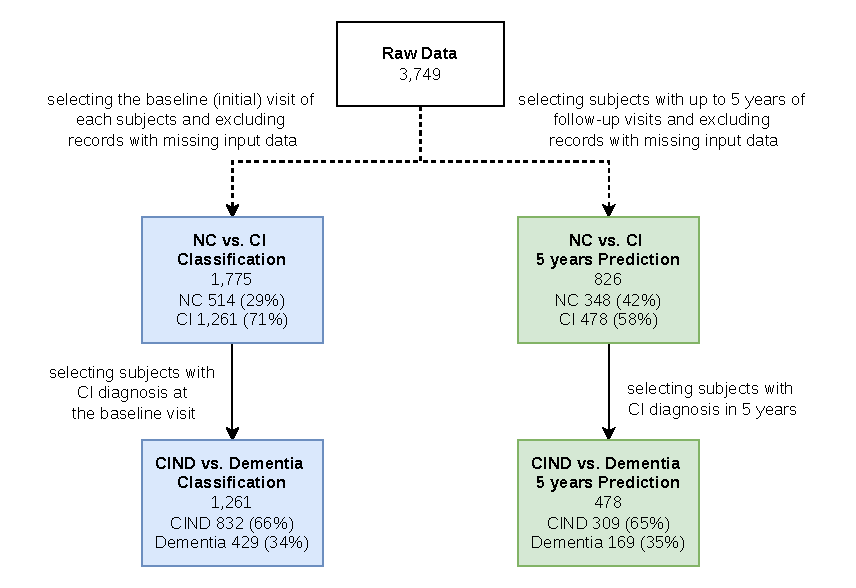
\includegraphics[width=0.7\textwidth]{figures/appendix/class-distribution-adni.pdf}
    \caption{The size of the data and the class distribution in the Alzheimer's Disease Neuroimaging Initiative (ADNI) external datasets}
    \label{fig:adni-data-stat}
\end{figure}

\begin{figure}[ht]
    \centering
    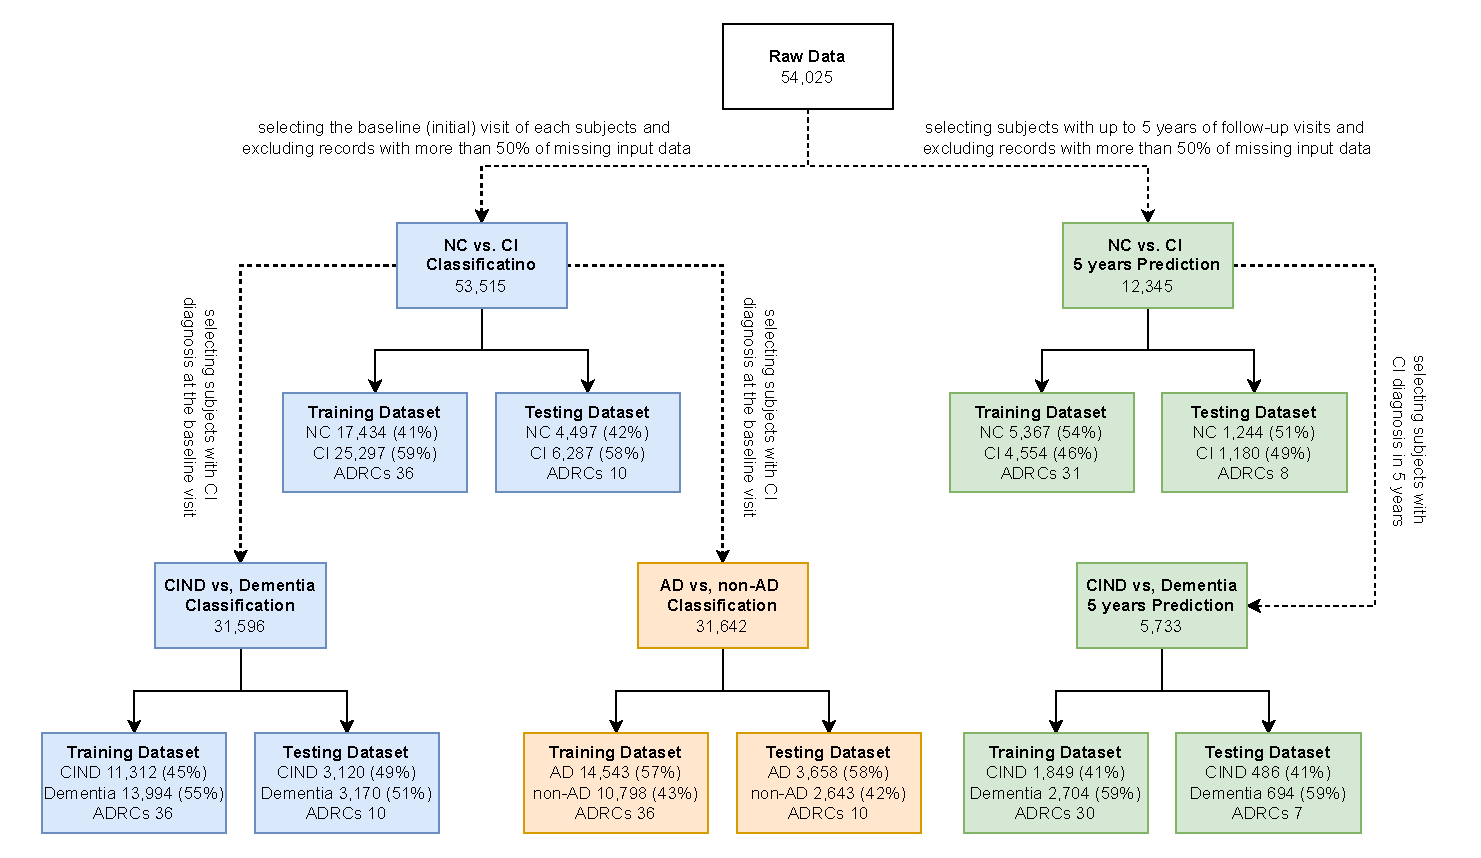
\includegraphics[width=1.0\textwidth]{figures/appendix/class-distribution-nacc.pdf}
    \caption{The size of the data and the class distribution in the NACC training and testing datasets}
    \begin{minipage}{\textwidth}
      \footnotesize The diagram demonstrate the hierarchical selection of data and the data selection criteria in different classification and prediction tasks.\newline
      The training and testing datasets split was done based on Alzheimer's disease research centers (\acrshort{ADRCs}) with 20\% ratio. The training dataset was collected from ADRCs that were not involved in the collection of the holdout testing dataset. The training and testing ADCRs in the NC vs. CI tasks are the same in the following CIND vs. Dementia and AD vs. non-AD tasks.\newline
      The high prevalence of cognitive impairment (\acrshort{CI}) is because subjects participated in NACC study are actively looking for medical advice due to concern on Cognitive deterioration.
    \end{minipage}
    \label{fig:nacc-data-stat}
\end{figure}

\subsection{Feature Selection}\label{sec:feature-selection-apdx}
These features were excluded because they are not available in the Alzheimer's Disease Neuroimaging Initiative (\acrshort{ADNI}) dataset: NACCLIVS, INDEPEND, ABUSOTHR, HEARING, COMPORT, CDRLANG, DECSUB, and DECIN. Categorical features with a dominant category  accounting for 97\% of the samples are excluded. Table~\ref{table:excluded-dominant-features} lists the excluded categories for each classification task. The remaining features were applied to the feature selection method. Table~\ref{table:feature-details} provides details about the selected features in all classification tasks. The correlation of the selected features for each classification task is presented in Figure~\ref{figure:feature-correlation}.

\begin{table}[H]
    \centering
    \caption{List of the excluded features with a dominant category for each classification task}
    \newcolumntype{C}{>{\centering\arraybackslash}X}
    \begin{tabularx}{\textwidth}{|C|C|}
    \hline
        Task & Excluded Features \\ \hline
        NC vs. CI Classificationn & CVCHF, SEIZURES, PD, PDOTHR, NCOTHR \\ \hline
        CIND vs. Dementia Classificationn & CVCHF, PD \\ \hline
        NC vs. CI Prediction & CVCHF, SEIZURES, PD, PDOTHR, DEL, DELSEV, HALL, HALLSEV, ELAT, ELATSEV \\ \hline
        CIND vs. Dementia Prediction & CVCHF, SEIZURES, PD, PDOTHR, HALL, HALLSEV \\ \hline
        AD vs. non-AD Classification & CVCHF, PD \\ \hline
    \end{tabularx}
    \label{table:excluded-dominant-features}
\end{table}


\begin{longtable}{|M{2.5cm}|M{2.5cm}|M{2.5cm}|M{2.5cm}|M{3cm}|}

    \caption{Details of the selected features in all classification tasks}

    \\ \hline
    \textbf{Category} & \textbf{NACC Code} & \textbf{ADNI Code} & \textbf{Description} & \textbf{Categorical \newline Values\textsuperscript{1}}
    \\ \hline
    \endhead
 
    \hline
    \endfoot

    \hline
    \endlastfoot

     % --- Footnotes Section (appears only on the last page) ---
    \hline
    \multicolumn{5}{p{15cm}}{
        \footnotesize This table lists all the selected features across all classification tasks.\newline
        \textsuperscript{1}Continuous features such as age and body mass index (\acrshort{BMI}) do not have categorical values.
    }
    \endlastfoot
    \label{table:feature-details}

    % --- Demographics (3 rows) ---
    \multirow{7}{*}{\parbox{2.5cm}{Demographics}}
     & NACCAGE & entry\_age & Age & ~ \\ \cline{2-5}
     & SEX & PTGENDER & Sex & 0=Male, \newline 1=Female \\ \cline{2-5}
     & PRIMLANG & PTPLANG & Subject's primary language & 0=English, 1=Spanish, 2=Others \\ \hline

    % --- Physical Assessment (1 row) ---
    \multirow{1}{*}{\parbox{2cm}{Physical Assessment}} 
     & NACCBMI & calculated using VSHEIGHT and VSWEIGHT & Body Mass Index (\acrshort{BMI}) & ~ \\ \hline

    \clearpage
    
     % --- Neuropsychiatric Inventory Questionnaire (NPI-Q) (3 rows) ---
    \multirow{3}{*}{\parbox{2cm}{Neuro-psychiatric Inventory Questionnaire (\acrshort{NPI-Q})}} 
     & ANX & NPIE & Anxiety in the last month & \multirow{9}{*}{\parbox{3cm}{0=No, 1=Yes}} \\ \cline{2-4}
     & APP & NPIL & Appetite and eating changes in the last month & \\ \cline{2-4}
     & IRR & NPII & Irritability or lability in the last month & \\ \hline

    % --- Geriatric Depression Scale (GDS) (2 rows) ---
    \multirow{2}{*}{\parbox{2cm}{Geriatric Depression Scale (GDS)}} 
     & MEMPROB & GDMEMORY & Subject reported memory problem & 0=No, 1=Yes \\ \cline{2-5}
     & ENERGY & GDENERGY & Do you feel full of energy? & 0=Yes, 1=No \\ \hline

    % --- Functional Activities Questionnaire (FAQ) (9 rows) ---
    \multirow{9}{*}{\parbox{2cm}{Functional Activities Questionnaire (\acrshort{FAQ}) \newline Instrumental Activities of Daily Living (IADL)}} 
     & BILLS & FAQFINAN & Pay bills and track spending & \multirow{9}{*}{\parbox{3cm}{0=Normal, \newline 1=Never did, \newline 2=Has difficulty but does by self, \newline 3=Requires assistance, \newline 4=Dependent}} \\ \cline{2-4}
     & TAXES & FAQFORM & Assemble tax records & \\ \cline{2-4}
     & SHOPPING & FAQSHOP & Shop alone for necessities & \\ \cline{2-4}
     & GAMES & FAQGAME & Play a game of skill & \\ \cline{2-4}
     & EVENTS & FAQEVENT & Keep track of current events & \\ \cline{2-4}
     & PAYATTN & FAQTV & Pay attention to a conversation & \\ \cline{2-4}
     & REMDATES & FAQREM & Remember dates and appointments & \\ \cline{2-4}
     & TRAVEL & FAQTRAVL & Travel out of neighborhood & \\ \cline{2-4}
     & MEALPREP & FAQMEAL & Prepare a balanced meal & \\ \hline

    % --- Clinical Dementia Rating (CDR) (6 rows) ---
    \multirow{10}{*}{\parbox{2cm}{Clinical Dementia Rating (CDR)}} 
     & MEMORY & CDMEMORY & Memory &  \multirow{10}{*}{\parbox{3cm}{0=No impairment, 1=Questionable impairment, 2=Mild impairment, 3=Moderate impairment, 4=Severe impairment}} \\ \cline{2-4}
     & ORIENT & CDORIENT & Orientation & \\ \cline{2-4}
     & JUDGMENT & CDJUDGE & Judgment \& Problem Solving & \\ \cline{2-4}
     & COMMUN & CDCOMMUN & Community Affairs & \\ \cline{2-4}
     & HOMEHOBB & CDHOME & Home \& Hobbies & \\ \cline{2-4}
     & PERSCARE & CDCARE & Personal Care & \\ \hline

\end{longtable}

% First page - subfigures (a) and (b)
\begin{figure}[H]
    \centering
    \begin{minipage}{0.9\textwidth}
        \centering
        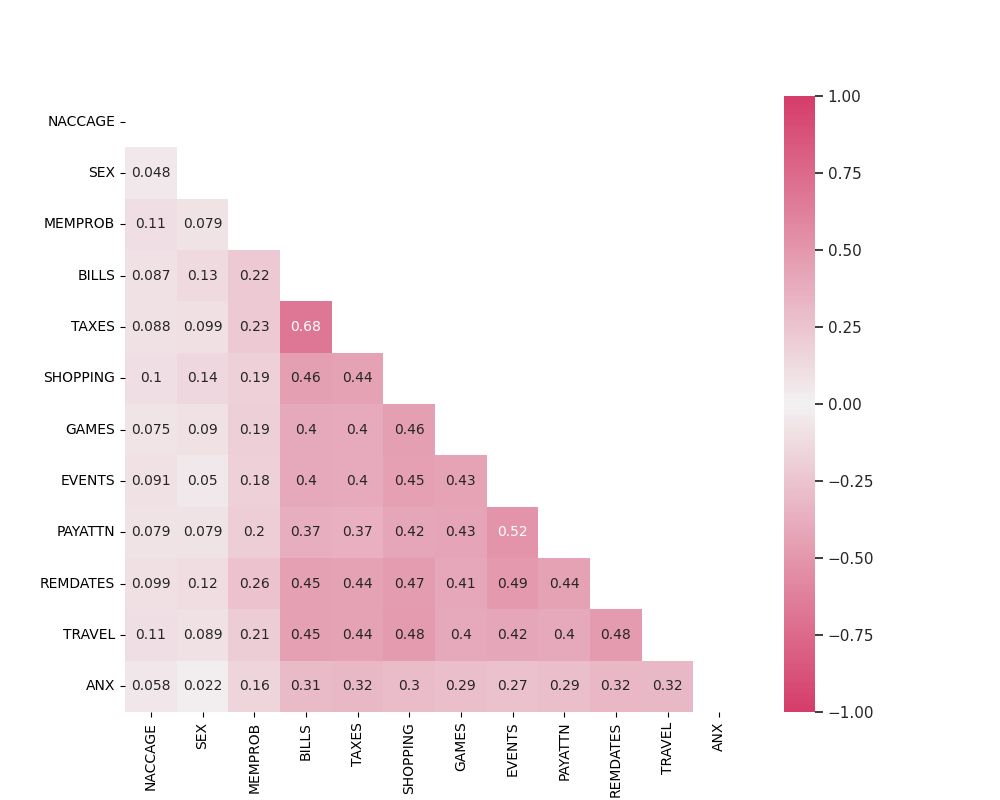
\includegraphics[width=\textwidth]{figures/appendix/impaired_classification_nacc_correlation_matrix.png}
        \caption*{(a) Feature correlation for the NC vs. CI classification task}
        \label{figure:feature-correlation-task1-apdx}
    \end{minipage}
    
    \vspace{0.5cm}
    
    \begin{minipage}{0.9\textwidth}
        \centering
        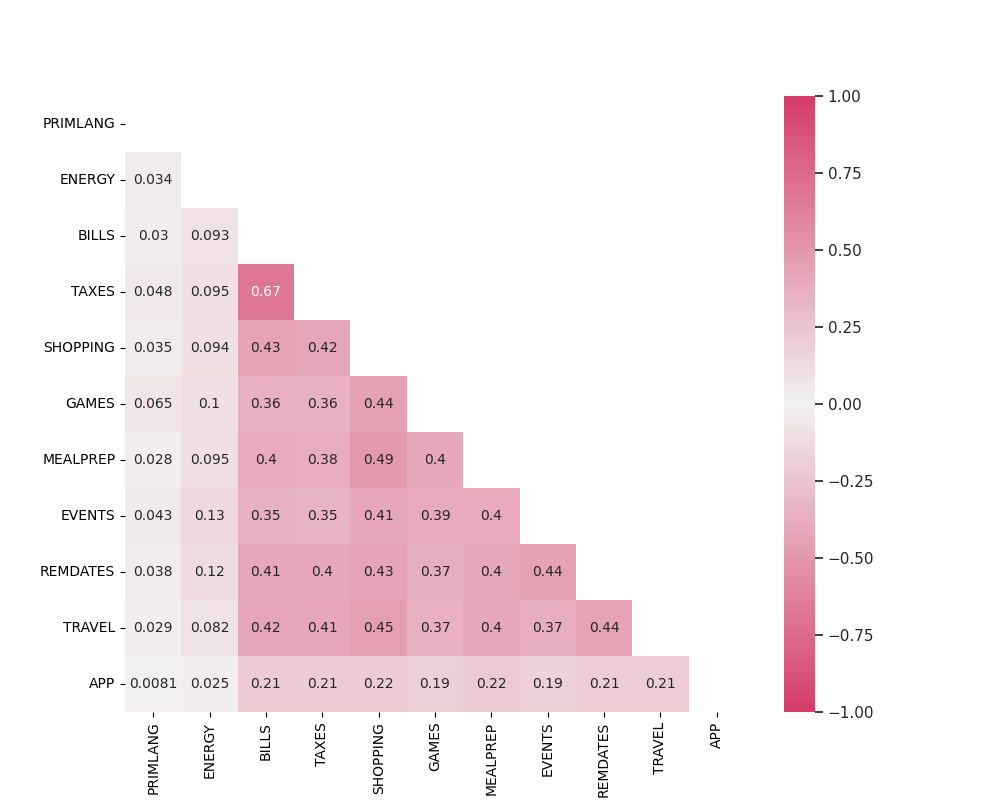
\includegraphics[width=\textwidth]{figures/appendix/dementia_classification_nacc_correlation_matrix.png}
        \caption*{(b) Feature correlation for the CIND vs. dementia classification task}
        \label{figure:feature-correlation-task2-apdx}
    \end{minipage}
    \caption{Feature correlation matrices for different classification and prediction tasks}
    \label{figure:feature-correlation}
\end{figure}

% Second page - subfigures (c) and (d)
\begin{figure}[H]
    \ContinuedFloat
    \centering
    \begin{minipage}{0.9\textwidth}
        \centering
        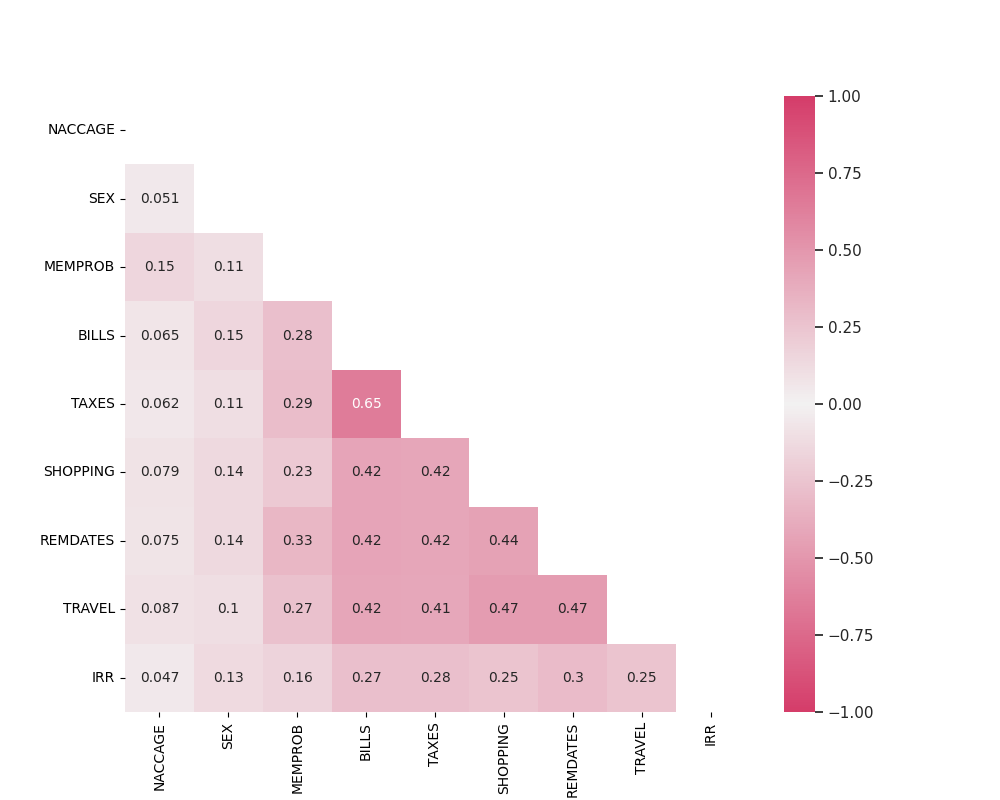
\includegraphics[width=\textwidth]{figures/appendix/impaired_prediction_nacc_correlation_matrix.png}
        \caption*{(c) Feature correlation for the future NC vs. CI prediction task}
        \label{figure:feature-correlation-task3-apdx}
    \end{minipage}
    
    \vspace{0.5cm}
    
    \begin{minipage}{0.9\textwidth}
        \centering
        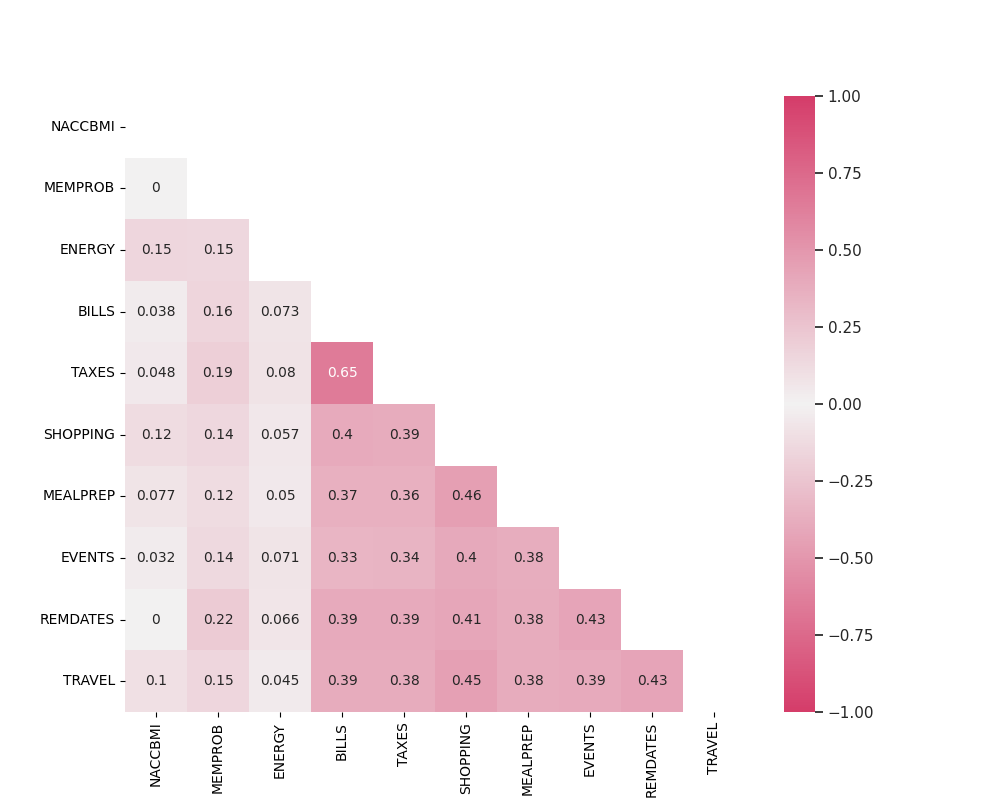
\includegraphics[width=\textwidth]{figures/appendix/dementia_prediction_nacc_correlation_matrix.png}
        \caption*{(d) Feature correlation for the future CIND vs. dementia prediction task}
        \label{figure:feature-correlation-task4-apdx}
    \end{minipage}
    \caption*{Figure \ref{figure:feature-correlation}: Feature correlation matrices for different classification and prediction tasks, continued}
\end{figure}

% Third page - subfigure (e)
\begin{figure}[H]
    \ContinuedFloat
    \centering
    \begin{minipage}{0.9\textwidth}
        \centering
        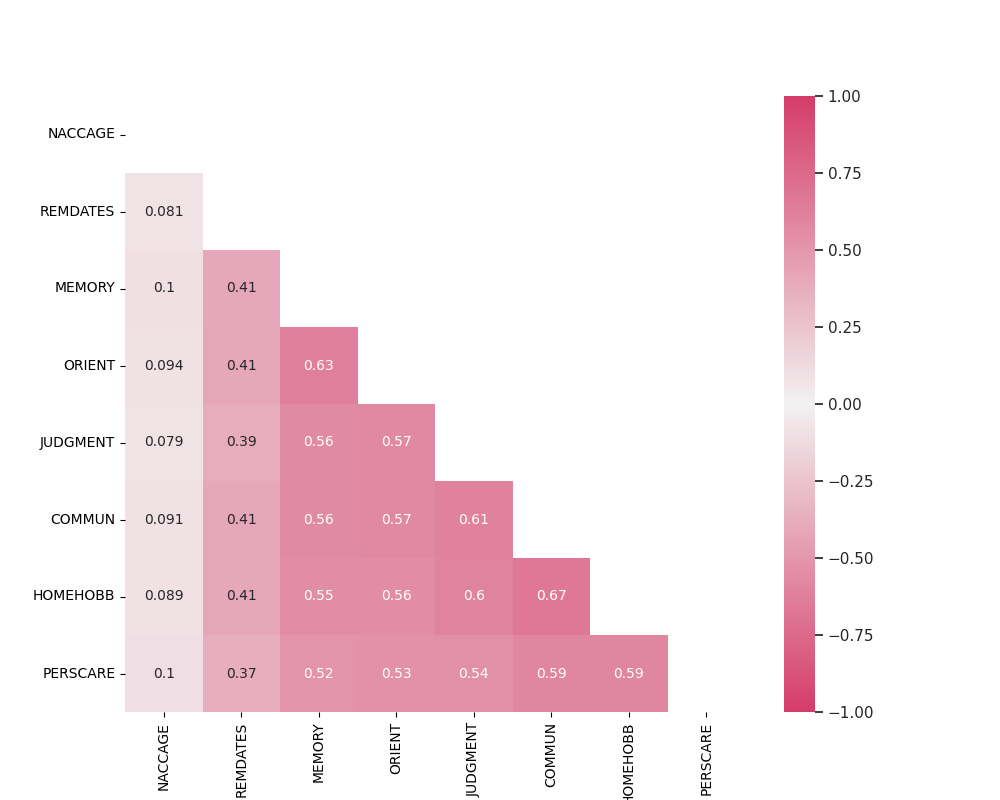
\includegraphics[width=\textwidth]{figures/appendix/type_classification_nacc_correlation_matrix.png}
        \caption*{(e) Feature correlation for the AD vs. non-AD classification task}
        \label{figure:feature-correlation-task5-apdx}
    \end{minipage}
    \caption*{Figure \ref{figure:feature-correlation}: Feature correlation matrices for different classification and prediction tasks (concluded)}
\end{figure}

\section{Supplementary Results of the Logisitic Regression Model Fine-tuning}\label{sec:lr-fine-tuning-apdx}
This section provides supplementary results of the hyperparameters fine-tuning of the selected logisitc regression (\acrshort{LR}) models. The optimization process only fine-tuned the \textit{C} parameter (inverse of the regularization strength). This hyperparameter controls the strength of regularization, which adjusts the balance between model simplicity and prediction accuracy. The \textit{lbfgs} solver was selected as the fixed optimization method due to its computational efficiency and stability for the given dataset size. In addition, the \textit{L2} penalty was exclusively employed. Since a rigorous feature selection phase was already completed prior to this stage, the automatic feature removal capability of the \textit{L1} penalty was not required. Instead, the \textit{L2} penalty was considered sufficient to prevent the model from overfitting and memorizing noise. The following tables (Tables \ref{table:lr-fine-tune-task1-apdx} to \ref{table:lr-fine-tune-task5-apdx}) present the performance and throughput of fine-tuned LR models in all classification tasks. The results demonstrate the ability of the proposed cost-effective model selection algorithm in selecting models that offer the highest efficiency while maintaining a high level of performance.


\begin{table}[H]
    \centering
    \caption{The hyperparameter fine-tuning of the logistic regression model for the NC vs. CI classification task}
    \begin{tabular}{|c|c|c|c|c|M{2cm}|M{2cm}|}
    \hline
        C & F1-score & G-mean & Sensitivity & Specificity & Training Throughput & Prediction Throughput \\ \hline
        5 & 0.848 & 0.842 & 0.785 & 0.903 & 1,511,839 \newline (1.07x) & 24,641,680\newline(1.09x) \\ \hline
        0.1 & 0.847 & 0.842 & 0.782 & 0.906 & 1,525,704\newline(1.08x) & 24,251,600\newline(1.07x) \\ \hline
        1 & 0.848 & 0.842 & 0.785 & 0.904 & 1,418,872 & 22,620,340 \\ \hline
        10 & 0.848 & 0.842 & 0.785 & 0.903 & 1,372,488\newline(0.97x) & 22,183,611\newline(0.98x) \\ \hline
        0.01c & 0.843 & 0.840 & 0.769 & 0.918 & 1,551,843\newline(1.09x) & 20,912,796\newline(0.92x) \\ \hline
    \multicolumn{7}{p{400pt}}{\footnotesize The \textit{C} parameter is the only fine-tuned hyperparameter. Default values are used for the other hyperparameters as defined in sklearn Python library. The most cost-effective model is when \textit{C} set as 5. This resulted in 1.07 increase in training throughput and 1.09 increase in prediction throughput as compared to the best performing model of \textit{C} equals 1 with similar level of performance.}
    \end{tabular}
    \label{table:lr-fine-tune-task1-apdx}
\end{table}

\begin{table}[H]
    \centering
    \caption{The hyperparameter fine-tuning of the logistic regression model for the CIND vs. dementia classification task}
    \begin{tabular}{|c|c|c|c|c|M{2cm}|M{2cm}|}
    \hline
        C & F1-score & G-mean & Sensitivity & Specificity & Training Throughput & Prediction Throughput \\ \hline
        0.01 & 0.842 & 0.828 & 0.827 & 0.830 & 512,085 & 19,831,465 \\ \hline
        0.1 & 0.842 & 0.828 & 0.827 & 0.829 & 434,190 (0.85x) & 17,929,038 (0.90x) \\ \hline
        1 & 0.842 & 0.828 & 0.827 & 0.829 & 565,870 (1.11x) & 17,314,929 (0.87x) \\ \hline
        5 & 0.842 & 0.828 & 0.827 & 0.829 & 579,724 (1.13x) & 17,300,820 (0.87x) \\ \hline
        10 & 0.842 & 0.828 & 0.827 & 0.829 & 586,756 (1.15x) & 17,351,721 (0.87x) \\ \hline
    \multicolumn{7}{p{400pt}}{\footnotesize The \textit{C} parameter is the only fine-tuned hyperparameter. Default values are used for the other hyperparameters as defined in sklearn Python library. The most cost-effective model is when \textit{C} set as 0.01.}
    \end{tabular}
    \label{table:lr-fine-tune-task2-apdx}
\end{table}

\begin{table}[H]
    \centering
    \caption{The hyperparameter fine-tuning of the logistic regression model for the future NC vs. CI prediction task}
    \begin{tabular}{|c|c|c|c|c|M{2cm}|M{2cm}|}
    \hline
        C & F1-score & G-mean & Sensitivity & Specificity & Training Throughput & Prediction Throughput \\ \hline
        5 & 0.747 & 0.770 & 0.723 & 0.820 & 819,113 (1.04x) & 6,630,848 (1.07x) \\ \hline
        0.1 & 0.747 & 0.771 & 0.718 & 0.828 & 784,029 & 6,173,582 \\ \hline
        1 & 0.747 & 0.770 & 0.723 & 0.821 & 755,493 (0.96x) & 6,543,298 (0.99x) \\ \hline
        10 & 0.747 & 0.770 & 0.723 & 0.820 & 783,967 (0.99x) & 7,094,149 (1.07x) \\ \hline
        0.01 & 0.744 & 0.770 & 0.692 & 0.858 & 885,304 (1.13x) & 5,473,828 (0.83x) \\ \hline
    \multicolumn{7}{p{400pt}}{\footnotesize The \textit{C} parameter is the only fine-tuned hyperparameter. Default values are used for the other hyperparameters as defined in sklearn Python library. The most cost-effective model is when \textit{C} set as 5. This resulted in 1.04 increase in training throughput and 1.07 increase in prediction throughput as compared to the best performing model of \textit{C} equals 0.1 with similar level of performance.}
    \end{tabular}
    \label{table:lr-fine-tune-task3-apdx}
\end{table}

\begin{table}[H]
    \centering
    \caption{The hyperparameter fine-tuning of the logistic regression model for the future CIND vs. dementia prediction task}
    \begin{tabular}{|c|c|c|c|c|M{2cm}|M{2cm}|}
    \hline
        C & F1-score & G-mean & Sensitivity & Specificity & Training Throughput & Prediction Throughput \\ \hline
        0.01 & 0.773 & 0.757 & 0.714 & 0.804 & 744,495 (1.14x) & 5,276,181 (1.41x) \\ \hline
        10 & 0.785 & 0.763 & 0.738 & 0.788 & 757,565 (1.16x) & 4,915,115 (1.32x) \\ \hline
        5 & 0.785 & 0.763 & 0.738 & 0.788 & 705,062 (1.08x) & 4,750,137 (1.27x) \\ \hline
        1 & 0.785 & 0.763 & 0.739 & 0.788 & 655,482 & 3,732,914 \\ \hline
        0.1 & 0.782 & 0.760 & 0.736 & 0.786 & 636,293 (0.97x) & 4,396,008 (1.18x) \\ \hline
    \multicolumn{7}{p{400pt}}{\footnotesize The \textit{C} parameter is the only fine-tuned hyperparameter. Default values are used for the other hyperparameters as defined in sklearn Python library. The most cost-effective model is when \textit{C} set as 0.01. This resulted in 1.14 increase in training throughput and 1.41 increase in prediction throughput as compared to the best performing model of \textit{C} equals 1 with similar level of performance.}
    \end{tabular}
    \label{table:lr-fine-tune-task4-apdx}
\end{table}

\begin{table}[H]
    \centering
    \caption{The hyperparameter fine-tuning of the logistic regression model for the AD vs. non-AD classification task}
    \begin{tabular}{|c|c|c|c|M{2cm}|M{2cm}|}
    \hline
        C & G-mean & Sensitivity & Specificity & Training Throughput & Prediction Throughput \\ \hline
        5 & 0.702 & 0.689 & 0.714 & 1,123,435 (1.34x) & 19,910,963 (1.20x) \\ \hline
        10 & 0.702 & 0.689 & 0.714 & 1,127,797 (1.35x) & 19,810,778 (1.20x) \\ \hline
        0.1 & 0.701 & 0.688 & 0.715 & 1,105,503 (1.32x) & 18,360,040 (1.11x) \\ \hline
        1 & 0.702 & 0.689 & 0.715 & 1,124,573 (1.34x) & 17,661,511 (1.07x) \\ \hline
        0.01 & 0.702 & 0.686 & 0.718 & 837,734 & 16,524,892 \\ \hline
    \multicolumn{6}{p{350pt}}{\footnotesize The \textit{C} parameter is the only fine-tuned hyperparameter. Default values are used for the other hyperparameters as defined in sklearn Python library. The most cost-effective model is when \textit{C} set as 5. This resulted in 1.34 increase in training throughput and 1.20 increase in prediction throughput as compared to the best performing model of \textit{C} equals 0.01 with similar level of performance.}
    \end{tabular}
    \label{table:lr-fine-tune-task5-apdx}
\end{table}

\section{Cost-effective Model Selection Algorithm Use Cases}\label{sec:selection-algorithm-usecases-apdx}
In order to demonstrate how the proposed model selection algorithm can help identify the most cost-effective model that aligns with specific use case requirements, Table~\ref{table:selection-algorithm-usecases} provides a comparison of performance and speed requirements across various use cases from different industries. It is important to note that the metrics and requirements presented in this table are mainly for illustrative purposes and should not be used as a definitive guide.

\begin{table}[!ht]
    \centering
    \caption{Comparison of performance and speed requirements across diverse use cases}
    \newcolumntype{C}{>{\centering\arraybackslash}X}
    \begin{tabularx}{\textwidth}{|C|C|C|C|C|}
    \hline
        \textbf{Use Case} & \textbf{Performance Metrics} & \textbf{Primary Metric} &  \textbf{Speed Requirement} & \textbf{Cost-effectiveness Requirement} \\ \hline
        Healthcare --- Disease Prediction & F2-score and Accuracy & F2-score & Prediction speed is more important than training speed & Minor decrease in performance for any degree of improvement in speed \\ \hline
        Finance --- Credit Scoring & F1-score and AUC & F1-score & Both training and prediction speed are equally important & Minor decrease in performance for high improvement in speed \\ \hline
        Retail --- Customer Churn Prediction & F1-score and Recall & F1-score & Prediction speed is more important than training speed & Minor decrease in performance for any degree of improvement in speed \\ \hline
        Manufacturing --- Fault Detection & F2-score & F2-score & Prediction speed is more important than training speed & Moderate decrease in performance for high improvement in speed \\ \hline
        Telecomm-unications --- Network Anomaly Detection & F2-score and AUC & F2-score & Both training and prediction speed are equally important & Moderate decrease in performance for high improvement in speed \\ \hline
    \end{tabularx}
    \label{table:selection-algorithm-usecases}
\end{table}

Each business use case has unique performance requirements that need to be taken into account when developing machine learning models. For the prediction of diseases in healthcare care, a high F2-score is essential to ensure that the models correctly identify positive cases. Therefore, the F2-score should be considered as the primary metric to assess such models. In retail, customer churn prediction models with high F1-score are crucial, especially in uneven class distributions. Recall can be used as a secondary metric to measure the model's ability to identify customers at risk of churn. On the other hand, the F2-score is considered the most critical performance metric to evaluate the ability of network anomaly detection models to identify as many anomalies as possible. The AUC is a valuable additional measure to distinguish between normal and anomalous activities. The machine learning model fine-tuning process can be complicated when multiple performance metrics are used to evaluate the models. Model developers can utilize the proposed model selection algorithm to simplify the process. The algorithm selects the best-performing model based on the defined performance metrics and their appropriate weights according to the unique use case requirements.

Besides performance, The speed of the machine learning models is another crucial evaluation metric for use cases requiring efficient solutions. The speed of the model may have an impact on the cost of training and using the model, especially if the model is developed and deployed in a cloud infrastructure. Different use cases may have different requirements for training and prediction speed. In healthcare, especially in disease prediction applications, the speed of prediction is critical to timely treatment decisions and to reduce the cost of widely serving the model. While training the model may be a time-consuming process, it typically occurs offline and does not directly impact patient care. In contrast, financial institutions often retrain credit scoring models to adapt to changing conditions. Therefore, it is important to have a fast training speed and prediction speed to enable quick responses. In other scenarios where machine learning models are being evaluated and optimized through multiple iterations and tests, such as model experiments in research, the speed of training is more crucial. Optimizing the model hyperparameters with different requirements of model training and prediction speed can be challenging and time-consuming. The proposed model selection algorithm automates the process by selecting models with the highest speed based on defined weights of training and prediction throughputs.

An ideal solution is one that delivers the desired results efficiently and effectively. There is often a delicate balance between model performance and efficiency, as highly performing models typically possess complex architectures that demand significant resources and time for training and inference. It is essential to select models that align with the specific performance and efficiency needs of the business use cases. Certain critical use cases, such as disease prediction, require highly accurate models, while model speed is also important in emergency situations. In these cases, an ideal model balances both factors without significantly sacrificing model performance. On the other hand, a model that is slightly less accurate but significantly faster can be a reliable option for applications that frequently scan large volumes of records, such as credit scoring models. There are other use cases where less accurate, yet admirably fast, models can be used. For instance, fault detection systems in manufacturing aim to quickly identify potential issues to prevent downtime. The speed of detection is crucial, even if it means having higher false positives, as it ensures immediate attention and further inspection. Selecting the appropriate model hyperparameters to achieve the desired level of performance and efficiency can be a challenging task. The proposed model selection algorithm can be useful in this regard. By transforming the model performance and efficiency requirements into preferred thresholds, the algorithm streamlines the selection of cost-effective models that align with the business needs.

\section{Supplementary Performance Results of the Selected Logistic Regression Model}
\label{sec:lr-complete-perf-apdx}
This section provides an extended report of the performance of the LR models. Tables \ref{table:lr-complete-perf-task1-apdx} to \ref{table:lr-complete-perf-task5-apdx} present the performance of the LR models in all classification tasks using additional metrics.

\begin{table}[H]
    \centering
    \caption{Extended performance metrics of the selected logistic regression model for the NC vs. CI classification task}
    \newcolumntype{C}{>{\centering\arraybackslash}X}
    \begin{tabularx}{\textwidth}{|C|C|C|C|}
    \hline
        \textbf{Metric} & \textbf{Internal Cross-Validation} & \textbf{NACC Cross-center Validation} & \textbf{ADNI External Validation} \\ \hline
        F1-score & 0.848 & 0.823 & 0.833 \\ \hline
        G-mean & 0.842 & 0.809 & 0.820 \\ \hline
        Precision & 0.922 & 0.874 & 0.953 \\ \hline
        Sensitivity & 0.785 & 0.777 & 0.739 \\ \hline
        Specificity & 0.903 & 0.843 & 0.911 \\ \hline
        Accuracy & 0.833 & 0.805 & 0.789 \\ \hline
        AUC & 0.844 & 0.810 & 0.825 \\ \hline
        AUPRC & 0.851 & 0.809 & 0.890 \\ \hline
        Kappa & 0.666 & 0.607 & 0.559 \\ \hline
    \multicolumn{4}{p{400pt}}{\footnotesize G-mean: geometric mean score, AUC: area under the curve, AUPRC: area under the precision-recall curve, Kappa: Cohen's kappa score.}
    \end{tabularx}
    \label{table:lr-complete-perf-task1-apdx}
\end{table}

\begin{table}[H]
    \centering
    \caption{Extended performance metrics of the selected logistic regression model for the CIND vs. dementia classification task}
    \newcolumntype{C}{>{\centering\arraybackslash}X}
    \begin{tabularx}{\textwidth}{|C|C|C|C|}
    \hline
        \textbf{Metric} & \textbf{Internal Cross-Validation} & \textbf{NACC Cross-center Validation} & \textbf{ADNI External Validation} \\ \hline
        F1-score & 0.842 & 0.837 & 0.777 \\ \hline
        G-mean & 0.828 & 0.826 & 0.840 \\ \hline
        Precision & 0.857 & 0.802 & 0.690 \\ \hline
        Sensitivity & 0.827 & 0.874 & 0.888 \\ \hline
        Specificity & 0.830 & 0.782 & 0.794 \\ \hline
        Accuracy & 0.828 & 0.828 & 0.826 \\ \hline
        AUC & 0.828 & 0.828 & 0.841 \\ \hline
        AUPRC & 0.804 & 0.765 & 0.651 \\ \hline
        Kappa & 0.654 & 0.656 & 0.638 \\ \hline
    \multicolumn{4}{p{400pt}}{\footnotesize G-mean: geometric mean score, AUC: area under the curve, AUPRC: area under the precision-recall curve, Kappa: Cohen's kappa score.}
    \end{tabularx}
    \label{table:lr-complete-perf-task2-apdx}
\end{table}

\begin{table}[H]
    \centering
    \caption{Extended performance metrics of the selected logistic regression model for the future NC vs. CI prediction task}
    \newcolumntype{C}{>{\centering\arraybackslash}X}
    \begin{tabularx}{\textwidth}{|C|C|C|C|}
    \hline
        \textbf{Metric} & \textbf{Internal Cross-Validation} & \textbf{NACC Cross-center Validation} & \textbf{ADNI External Validation} \\ \hline
        F1-score & 0.747 & 0.772 & 0.791 \\ \hline
        G-mean & 0.770 & 0.787 & 0.777 \\ \hline
        Precision & 0.774 & 0.829 & 0.844 \\ \hline
        Sensitivity & 0.723 & 0.721 & 0.745 \\ \hline
        Specificity & 0.820 & 0.859 & 0.810 \\ \hline
        Accuracy & 0.776 & 0.792 & 0.772 \\ \hline
        AUC & 0.772 & 0.790 & 0.778 \\ \hline
        AUPRC & 0.686 & 0.734 & 0.776 \\ \hline
        Kappa & 0.546 & 0.582 & 0.543 \\ \hline
    \multicolumn{4}{p{400pt}}{\footnotesize G-mean: geometric mean score, AUC: area under the curve, AUPRC: area under the precision-recall curve, Kappa: Cohen's kappa score.}
    \end{tabularx}
    \label{table:lr-complete-perf-task3-apdx}
\end{table}

\begin{table}[H]
    \centering
    \caption{Extended performance metrics of the selected logistic regression model for the future CIND vs. dementia prediction task}
    \newcolumntype{C}{>{\centering\arraybackslash}X}
    \begin{tabularx}{\textwidth}{|C|C|C|C|}
    \hline
        \textbf{Metric} & \textbf{Internal Cross-Validation} & \textbf{NACC Cross-center Validation} & \textbf{ADNI External Validation} \\ \hline
        F1-score & 0.773 & 0.811 & 0.715 \\ \hline
        G-mean & 0.757 & 0.803 & 0.780 \\ \hline
        Precision & 0.842 & 0.887 & 0.655 \\ \hline
        Sensitivity & 0.714 & 0.746 & 0.787 \\ \hline
        Specificity & 0.804 & 0.864 & 0.773 \\ \hline
        Accuracy & 0.750 & 0.795 & 0.778 \\ \hline
        AUC & 0.759 & 0.805 & 0.780 \\ \hline
        AUPRC & 0.771 & 0.811 & 0.591 \\ \hline
        Kappa & 0.500 & 0.591 & 0.536 \\ \hline
    \multicolumn{4}{p{400pt}}{\footnotesize G-mean: geometric mean score, AUC: area under the curve, AUPRC: area under the precision-recall curve, Kappa: Cohen's kappa score.}
    \end{tabularx}
    \label{table:lr-complete-perf-task4-apdx}
\end{table}

\begin{table}[H]
    \centering
    \caption{Extended performance metrics of the selected logistic regression model for the AD vs. non-AD classification task}
    \newcolumntype{C}{>{\centering\arraybackslash}X}
    \begin{tabularx}{\textwidth}{|C|C|C|}
    \hline
        \textbf{Metric} & \textbf{Internal Cross-Validation} & \textbf{NACC Cross-center Validation} \\ \hline
        F1-score & 0.725 & 0.706 \\ \hline
        G-mean & 0.702 & 0.670 \\ \hline
        Precision & 0.765 & 0.735 \\ \hline
        Sensitivity & 0.689 & 0.679 \\ \hline
        Specificity & 0.714 & 0.660 \\ \hline
        Accuracy & 0.700 & 0.671 \\ \hline
        AUC & 0.702 & 0.670 \\ \hline
        AUPRC & 0.705 & 0.686 \\ \hline
        Kappa & 0.397 & 0.334 \\ \hline
    \multicolumn{3}{p{400pt}}{\footnotesize G-mean: geometric mean score, AUC: area under the curve, AUPRC: area under the precision-recall curve, Kappa: Cohen's kappa score.}
    \end{tabularx}
    \label{table:lr-complete-perf-task5-apdx}
\end{table}

\section{Supplementary Results of Model Explainability}\label{sec:xai-apdx}
This section provides supplementary results related to the model explainability phase of this study. It is intended to support the findings that were discussed previously in the results and analysis chapter. The feature importance in the NACC cross-center validation and the ADNI external validation for all classification tasks is presented in Figures \ref{figure:summary-plot-task1-apdx} to \ref{figure:summary-plot-task5-apdx} together with summary plots demonstrating the direction of the impact of the features. Figures \ref{figure:dice-nacc-task1-apdx} to \ref{figure:dice-nacc-task4-apdx} display the quantity (the number of counterfactual examples generated per instance) and the sparsity (the number of features needed to be changed to generate the counterfactual examples) of the counterfactual explanation in the NACC cross-center validation, which can be compared with the corresponding metrics in the ADNI external validation that were provided previously in the results and analysis chapter. Tables \ref{table:cfe-adni-task1-apdx} to \ref{table:cfe-adni-task4-apdx} demonstrate samples of counterfactual examples generated in the ADNI external validation for all classification tasks to illustrate the feature changes required to reverse the predicted outcomes. The Diverse Counterfactual Explanations (\acrshort{DiCE}) with the \acrshort{KD-Tree} (K-dimensional tree) search method was used to generate the counterfactual examples for all classification tasks except the future CIND vs. dementia prediction task which used the random search method.

\begin{figure}[H]
    \centering
    \begin{minipage}{0.48\textwidth}
        \centering
        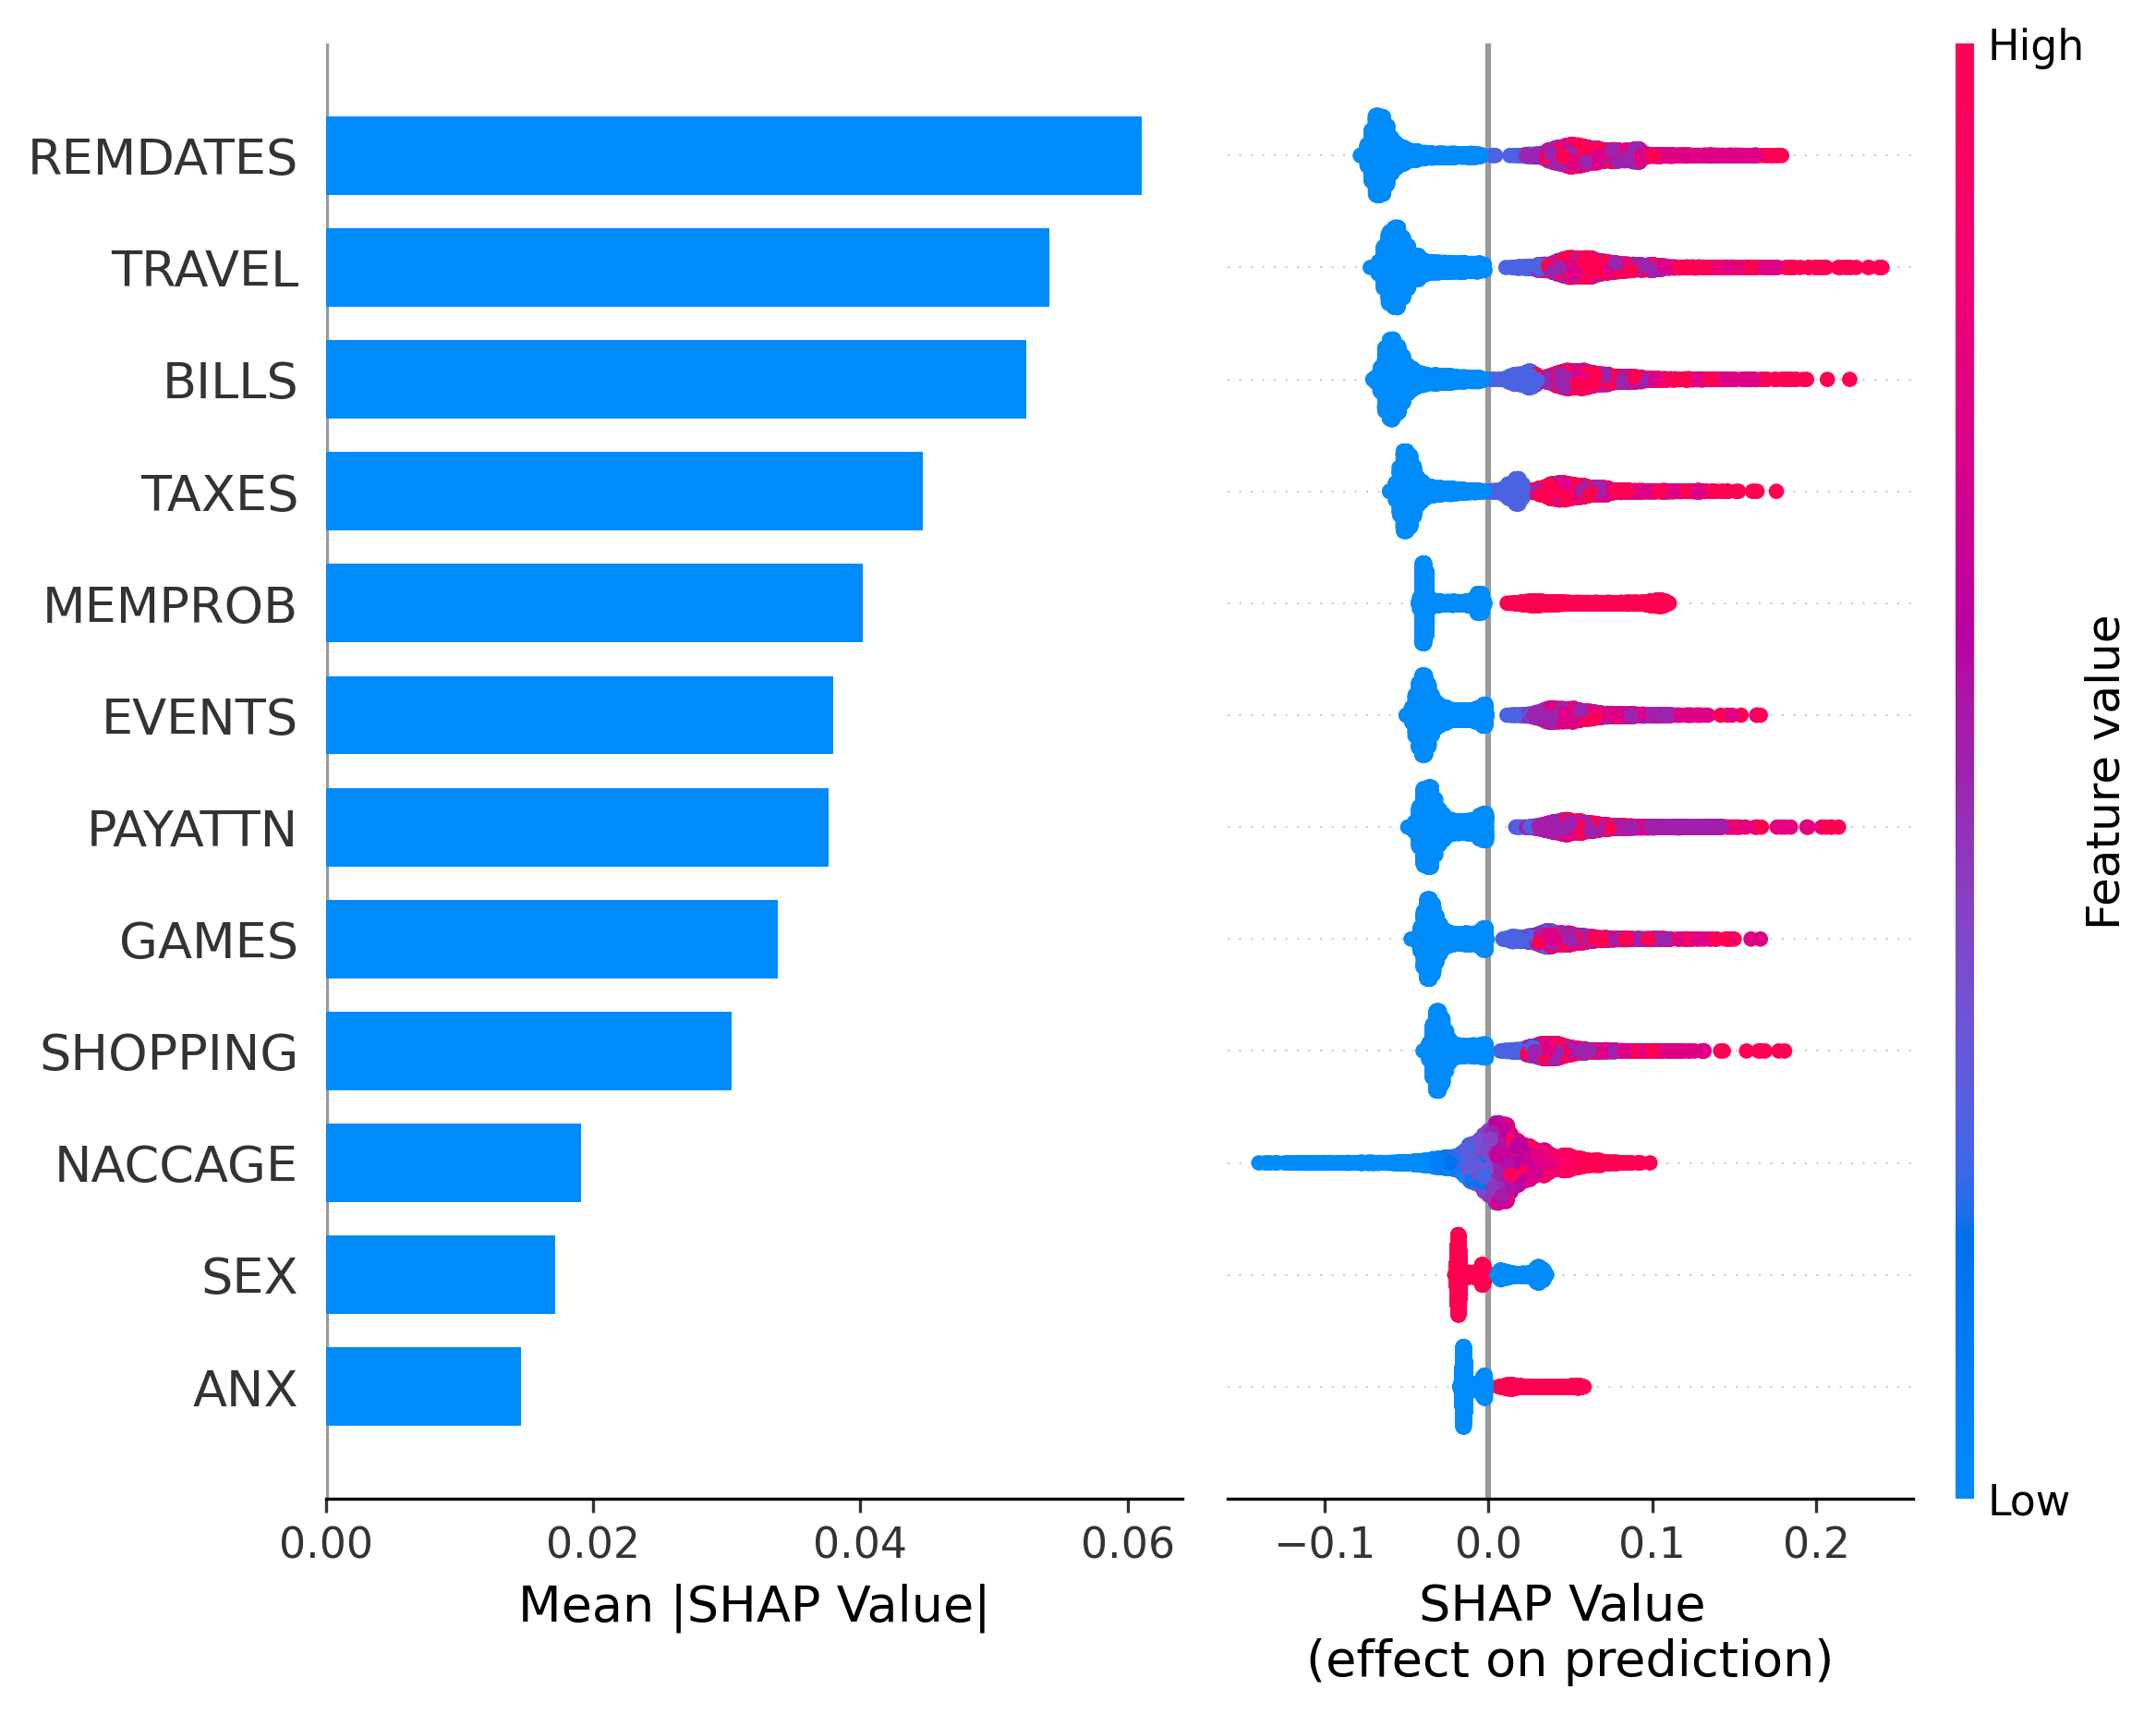
\includegraphics[width=\textwidth]{figures/appendix/impaired_classification_nacc_shap_feature_importance.png}
        \caption*{(a)  NACC cross-center validation}
    \end{minipage}
    \begin{minipage}{0.48\textwidth}
        \centering
        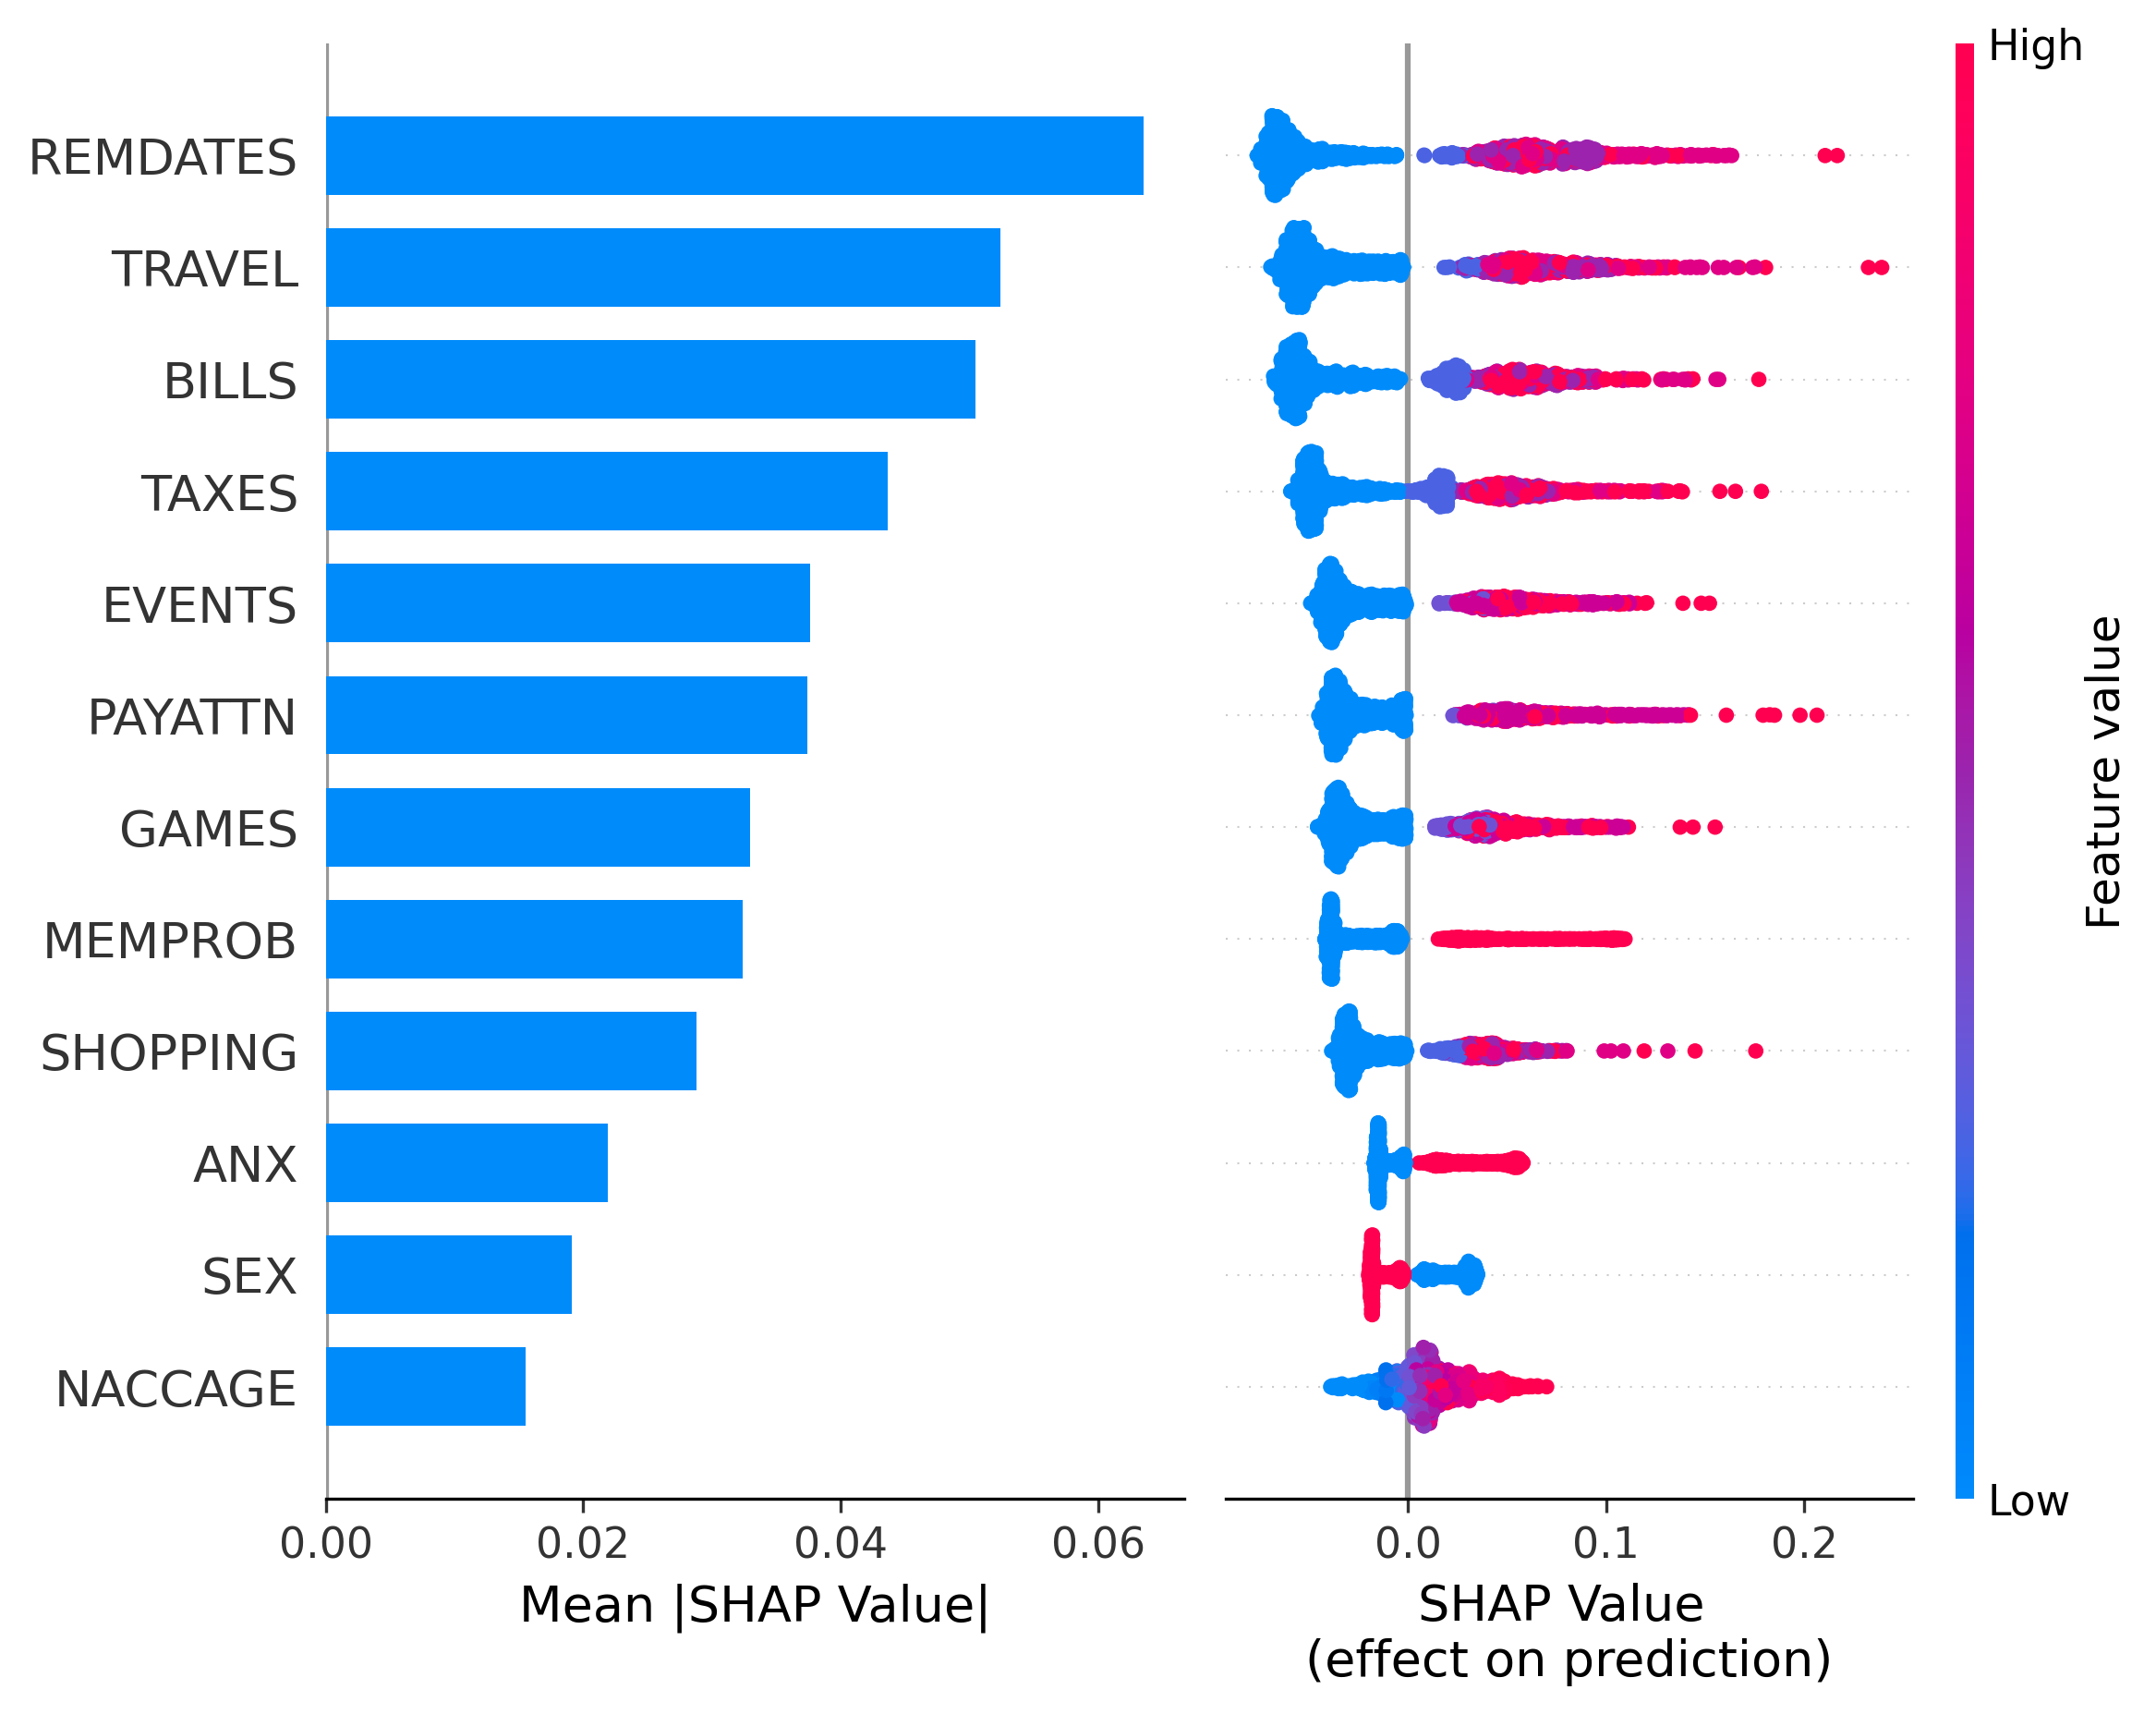
\includegraphics[width=\textwidth]{figures/appendix/impaired_classification_adni_shap_feature_importance.png}
        \caption*{(b) ADNI External Validation}
    \end{minipage}
    \caption{Feature importance with summary plot for the NC vs. CI classification task}
    \label{figure:summary-plot-task1-apdx}
\end{figure}

\begin{figure}[H]
    \centering
    \begin{minipage}{0.48\textwidth}
        \centering
        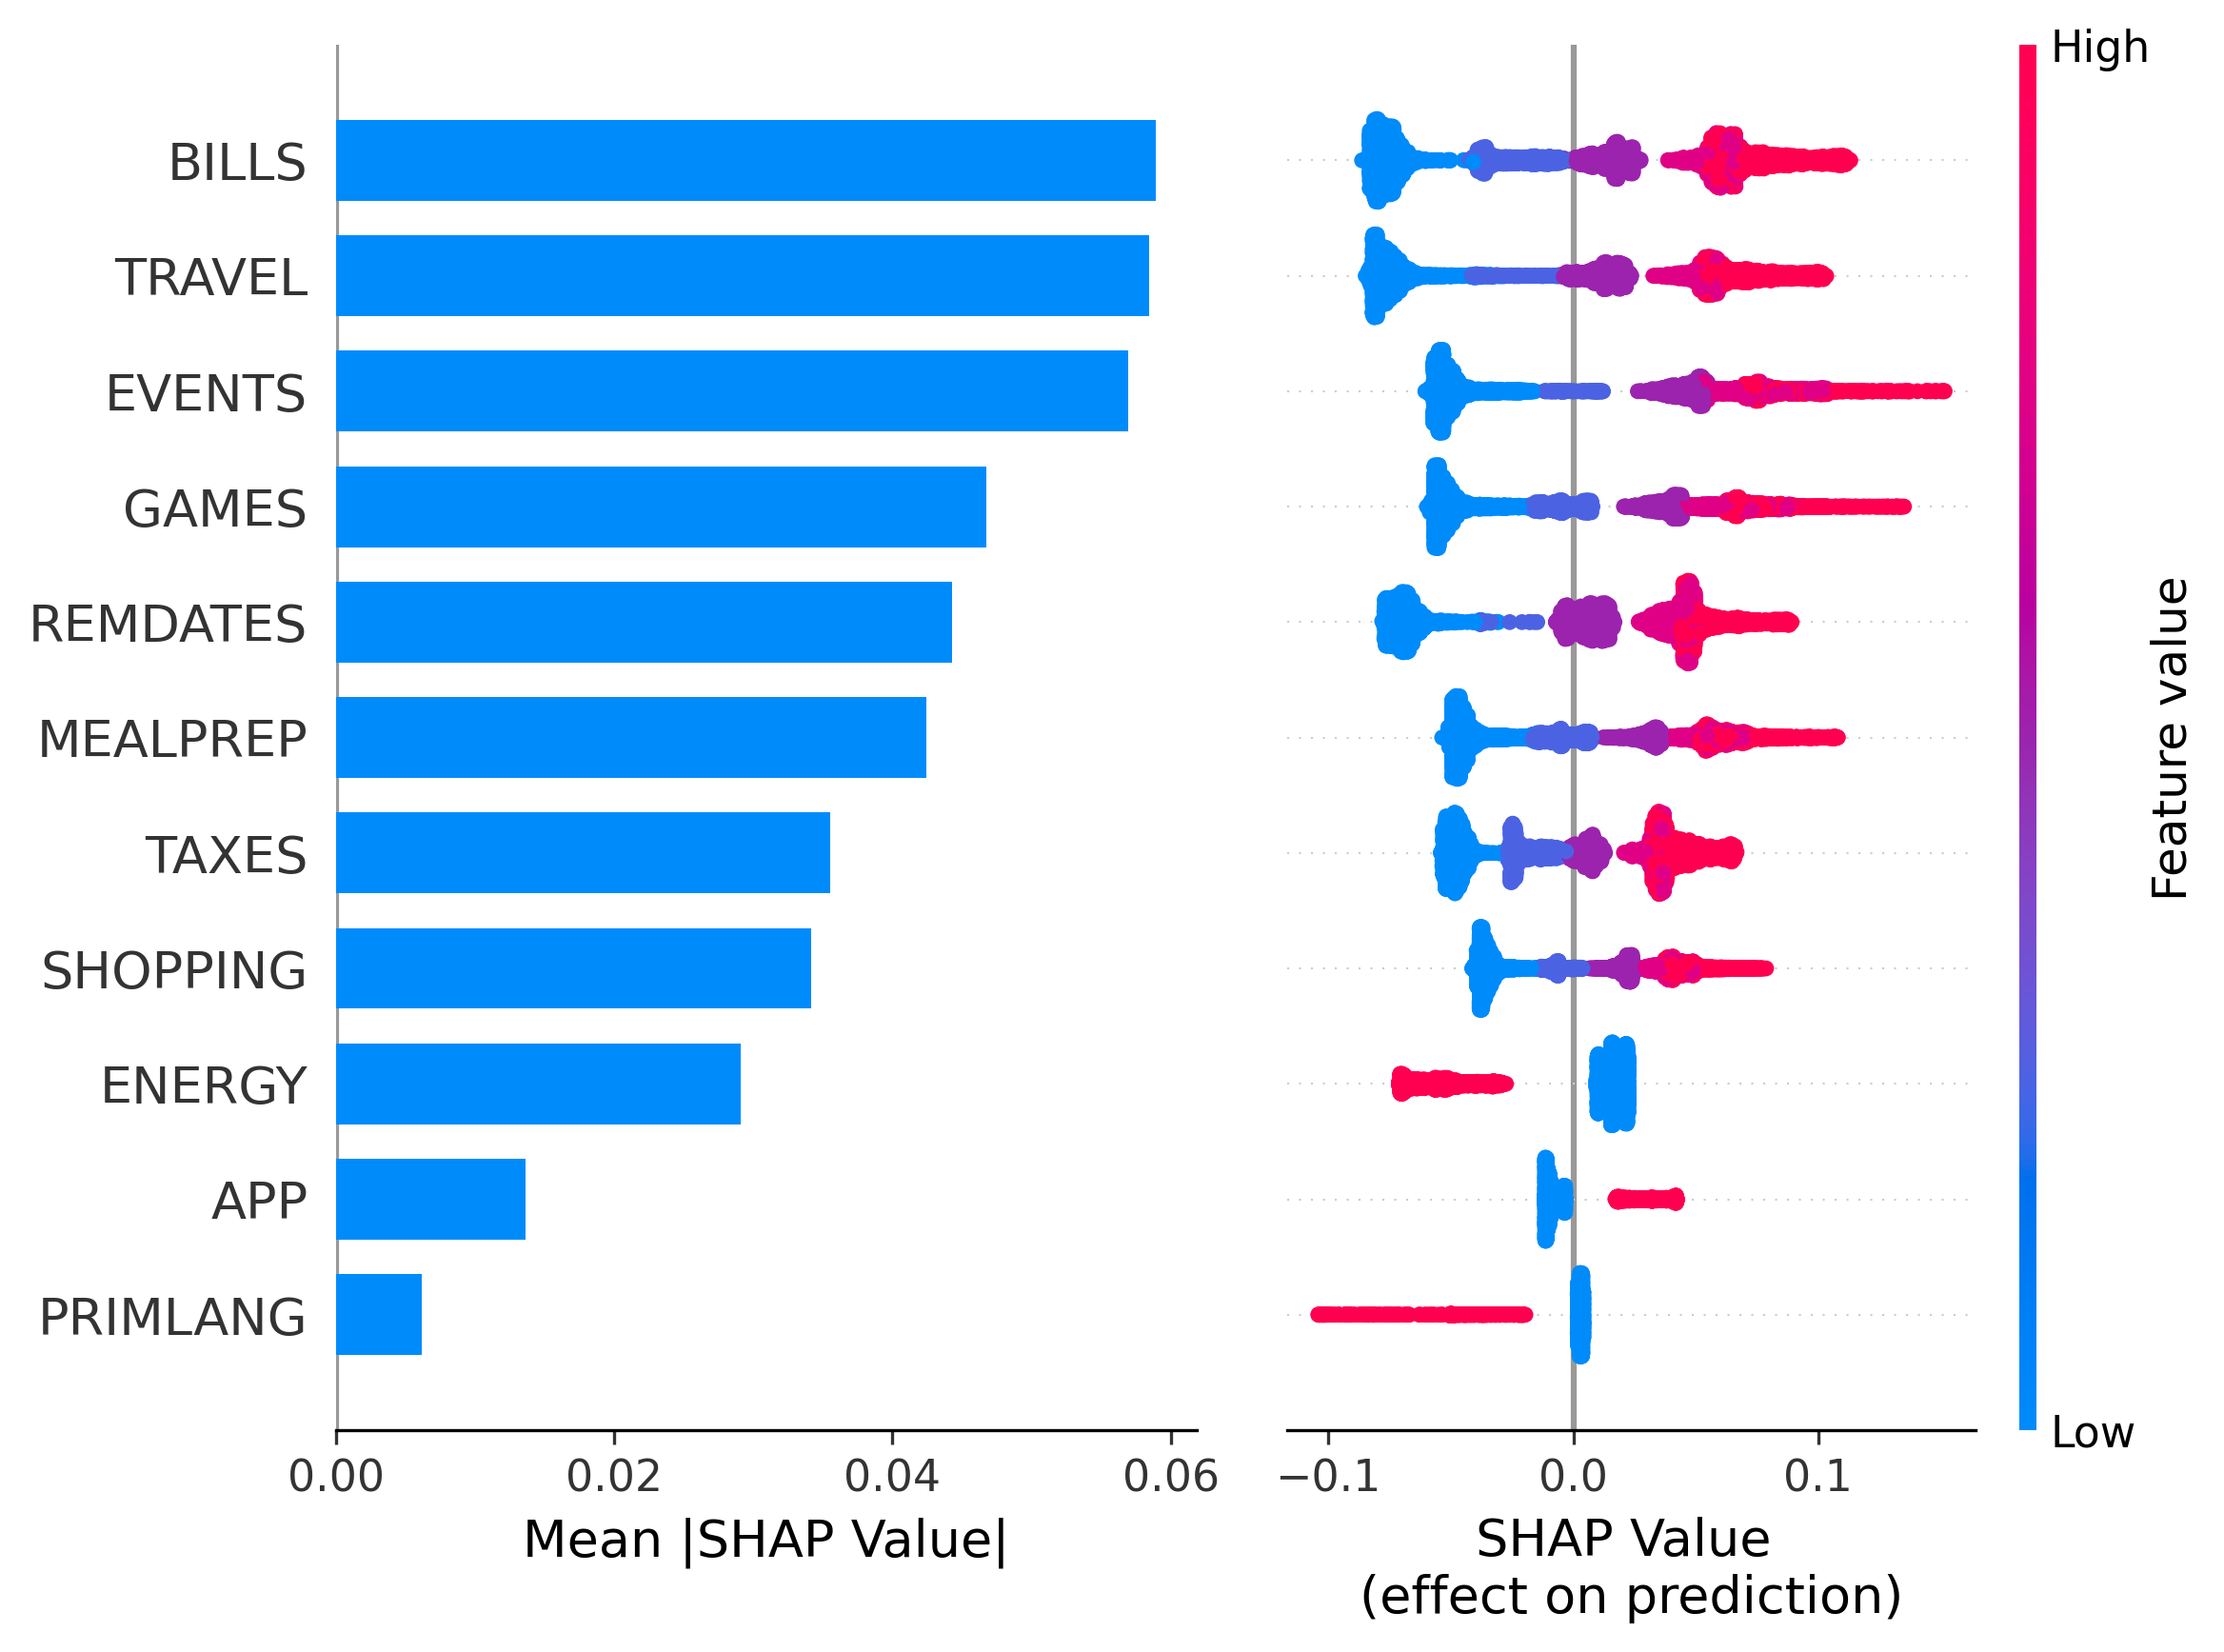
\includegraphics[width=\textwidth]{figures/appendix/dementia_classification_nacc_shap_feature_importance.png}
        \caption*{(a)  NACC cross-center validation}
    \end{minipage}
    \begin{minipage}{0.48\textwidth}
        \centering
        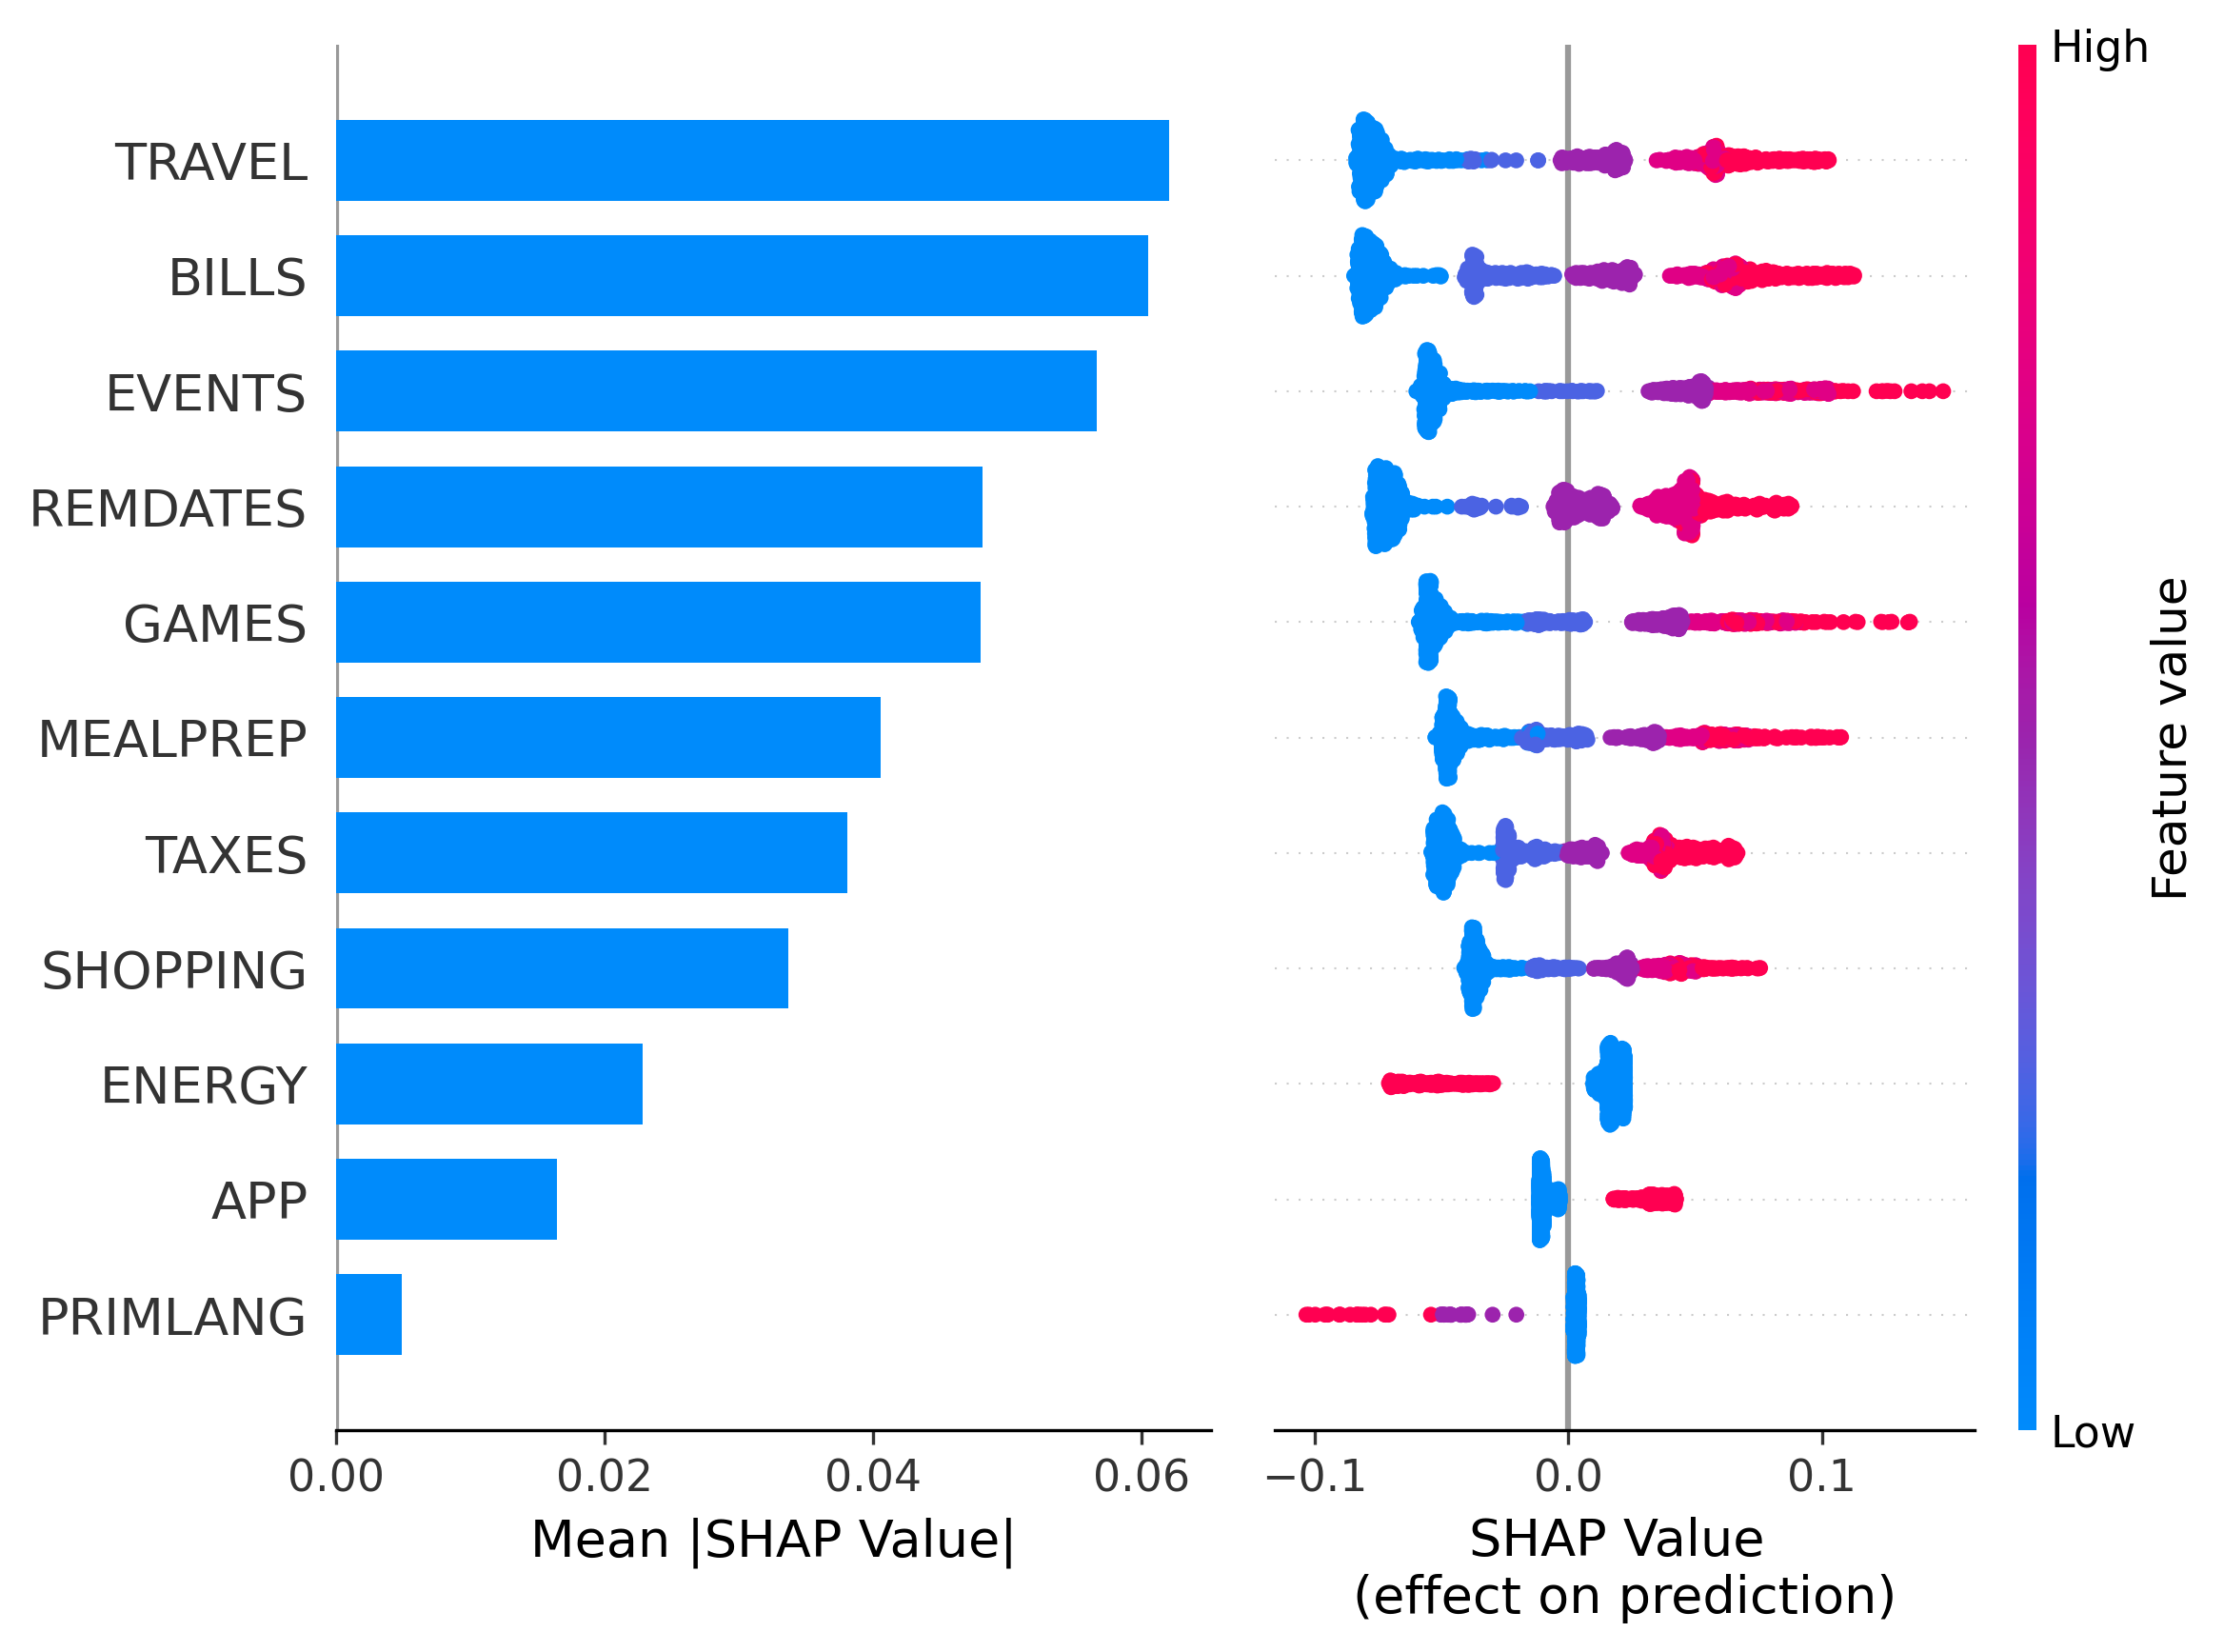
\includegraphics[width=\textwidth]{figures/appendix/dementia_classification_adni_shap_feature_importance.png}
        \caption*{(b) ADNI External Validation}
    \end{minipage}
    \caption{Feature importance with summary plot for the CIND vs. dementia classification task}
    \label{figure:summary-plot-task2-apdx}
\end{figure}

\begin{figure}[H]
    \centering
    \begin{minipage}{0.48\textwidth}
        \centering
        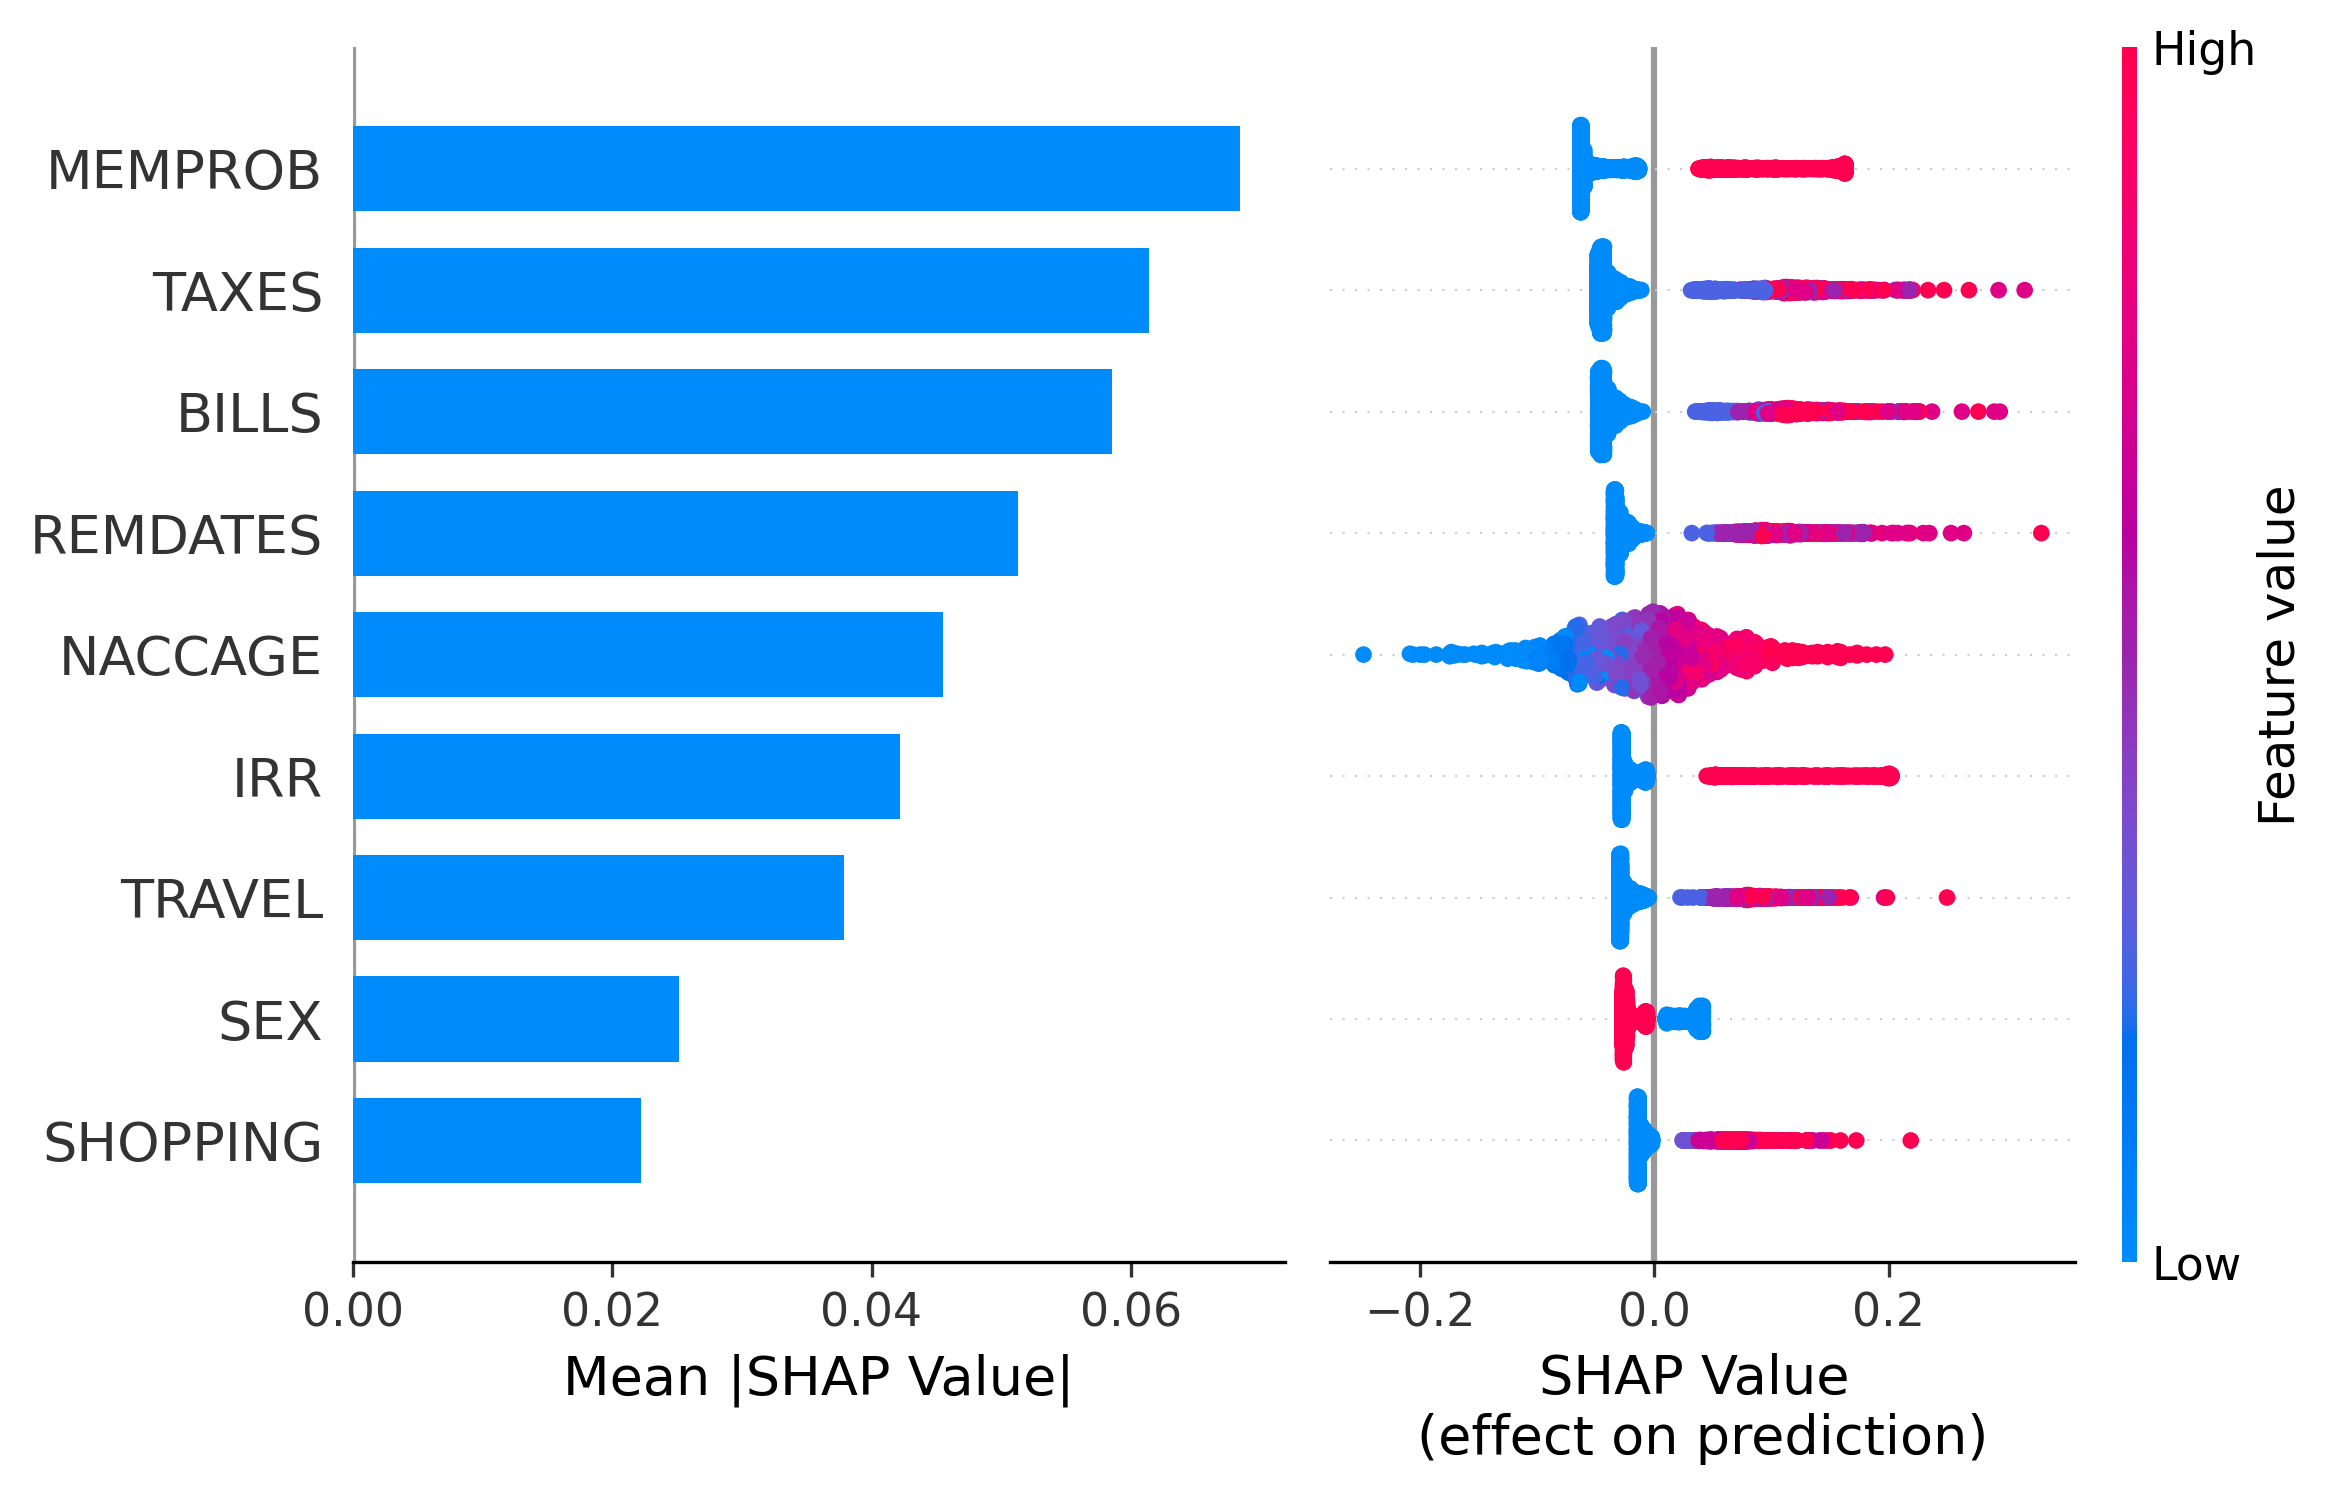
\includegraphics[width=\textwidth]{figures/appendix/impaired_prediction_nacc_shap_feature_importance.png}
        \caption*{(a)  NACC cross-center validation}
    \end{minipage}
    \begin{minipage}{0.48\textwidth}
        \centering
        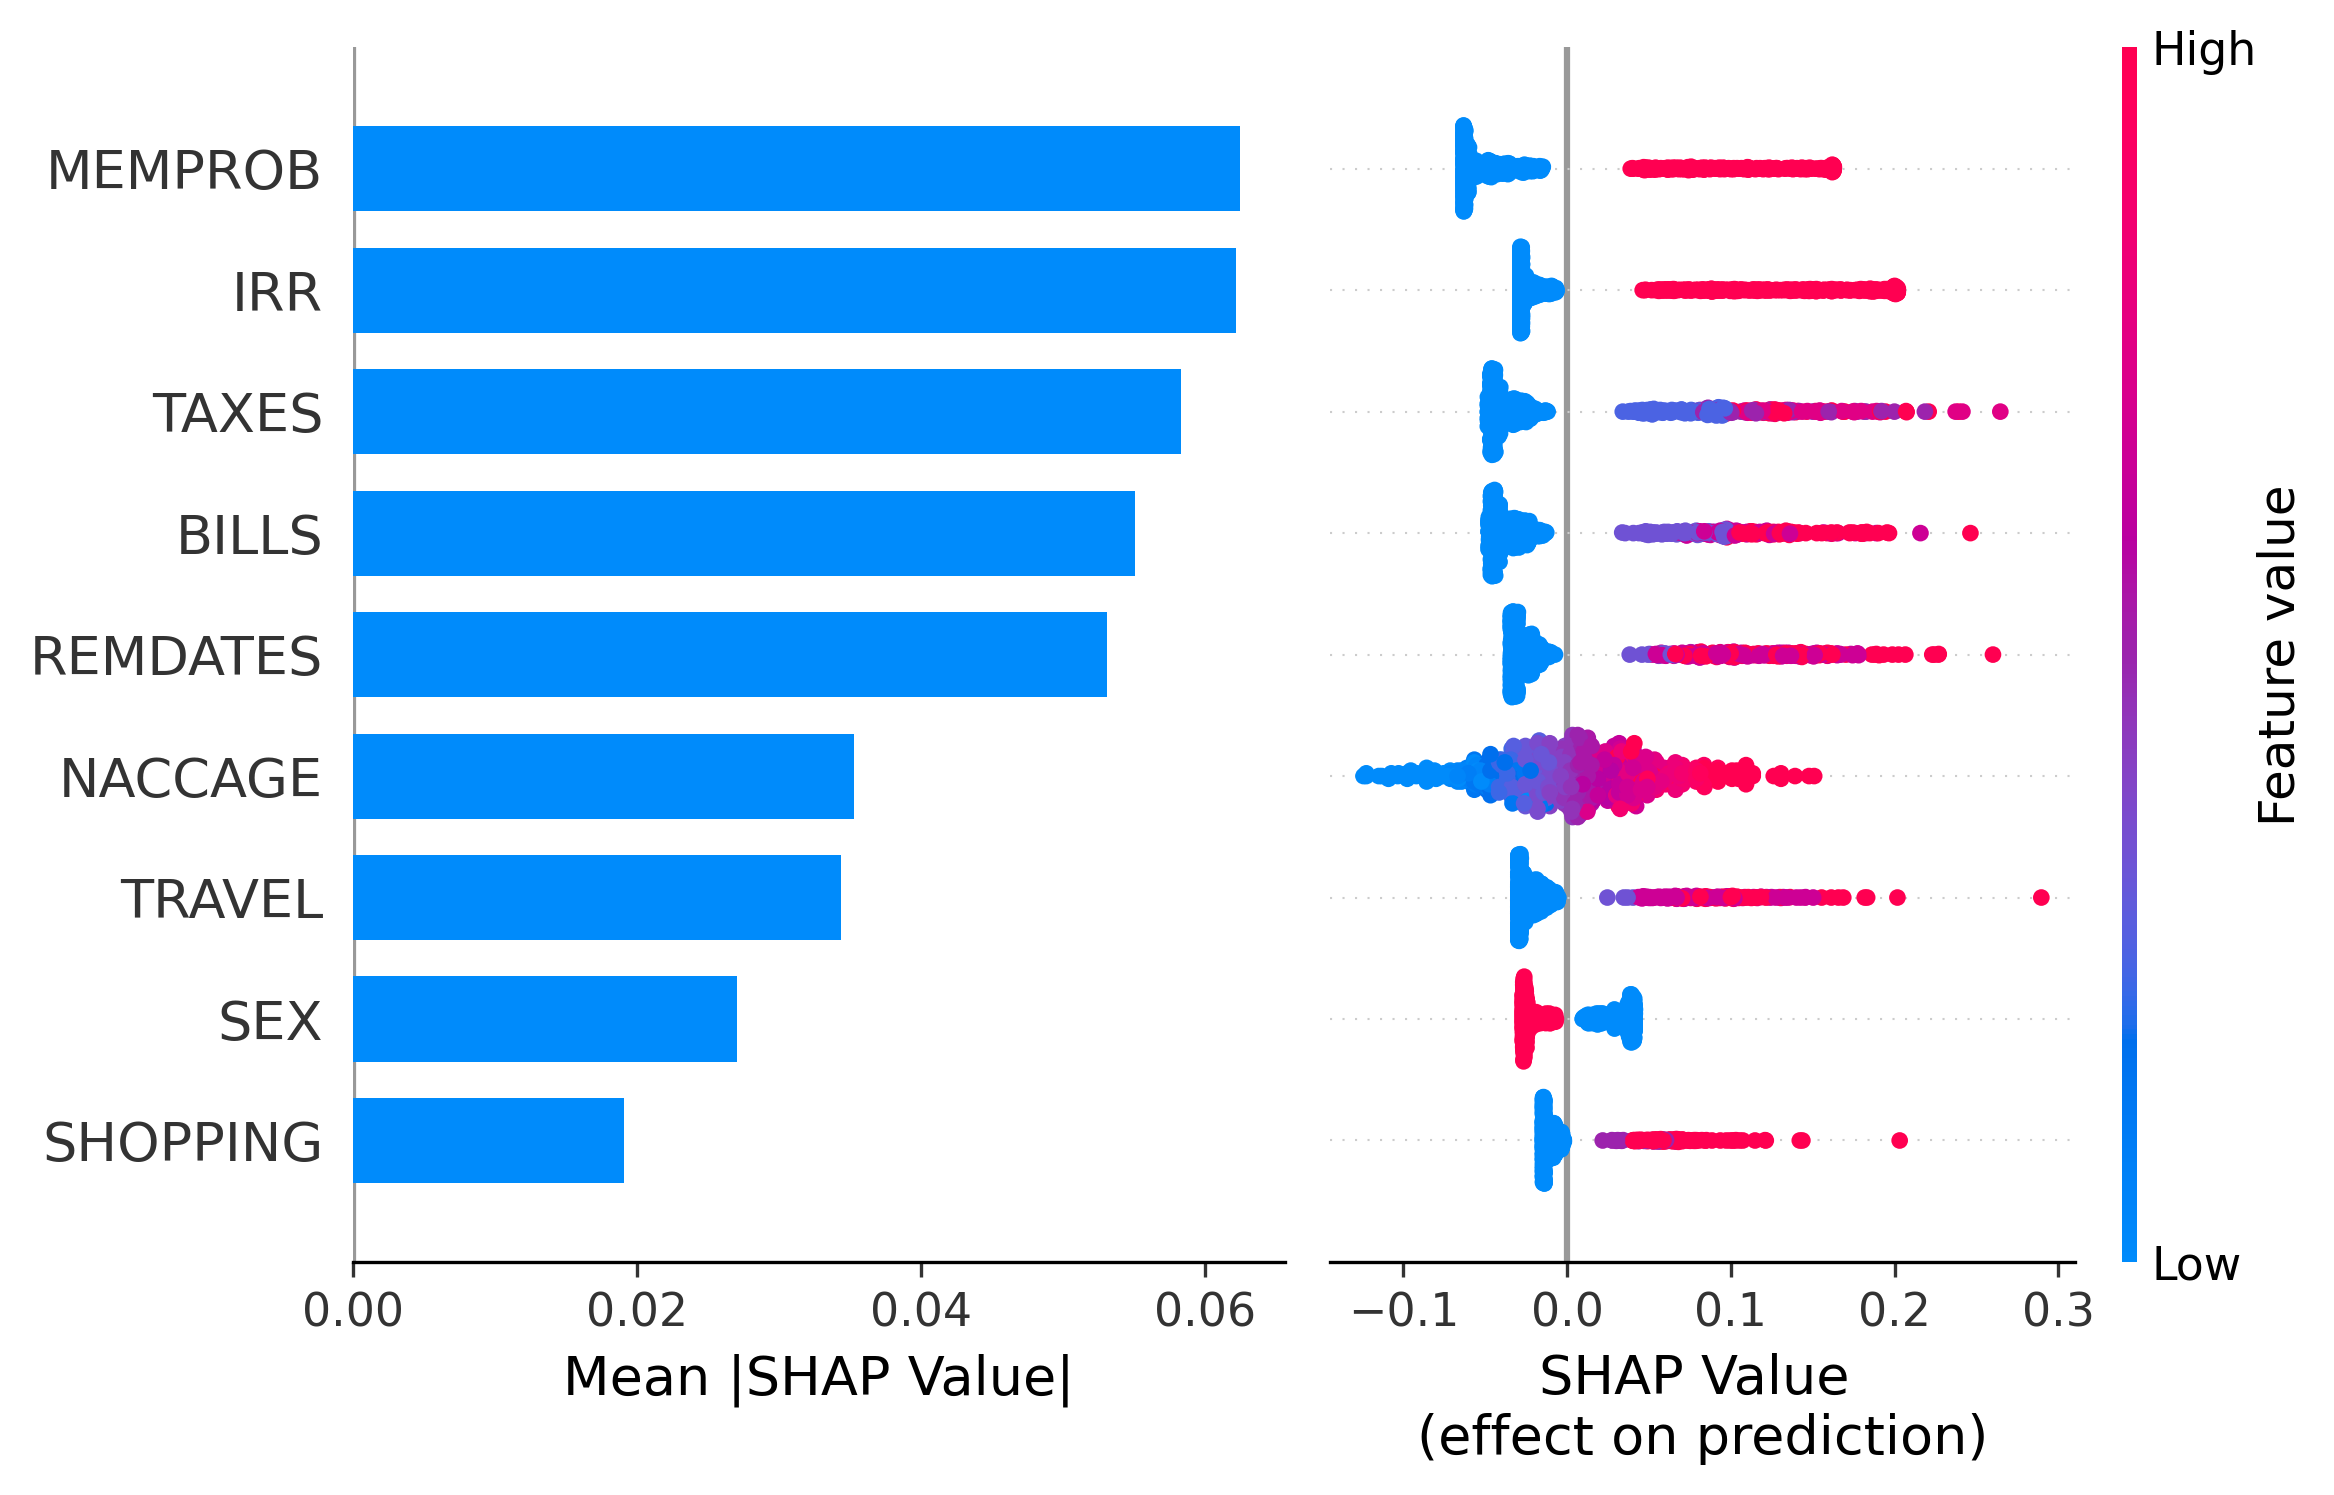
\includegraphics[width=\textwidth]{figures/appendix/impaired_prediction_adni_shap_feature_importance.png}
        \caption*{(b) ADNI External Validation}
    \end{minipage}
    \caption{Feature importance with summary plot for the feature NC vs. CI prediction task}
    \label{figure:summary-plot-task3-apdx}
\end{figure}

\begin{figure}[H]
    \centering
    \begin{minipage}{0.48\textwidth}
        \centering
        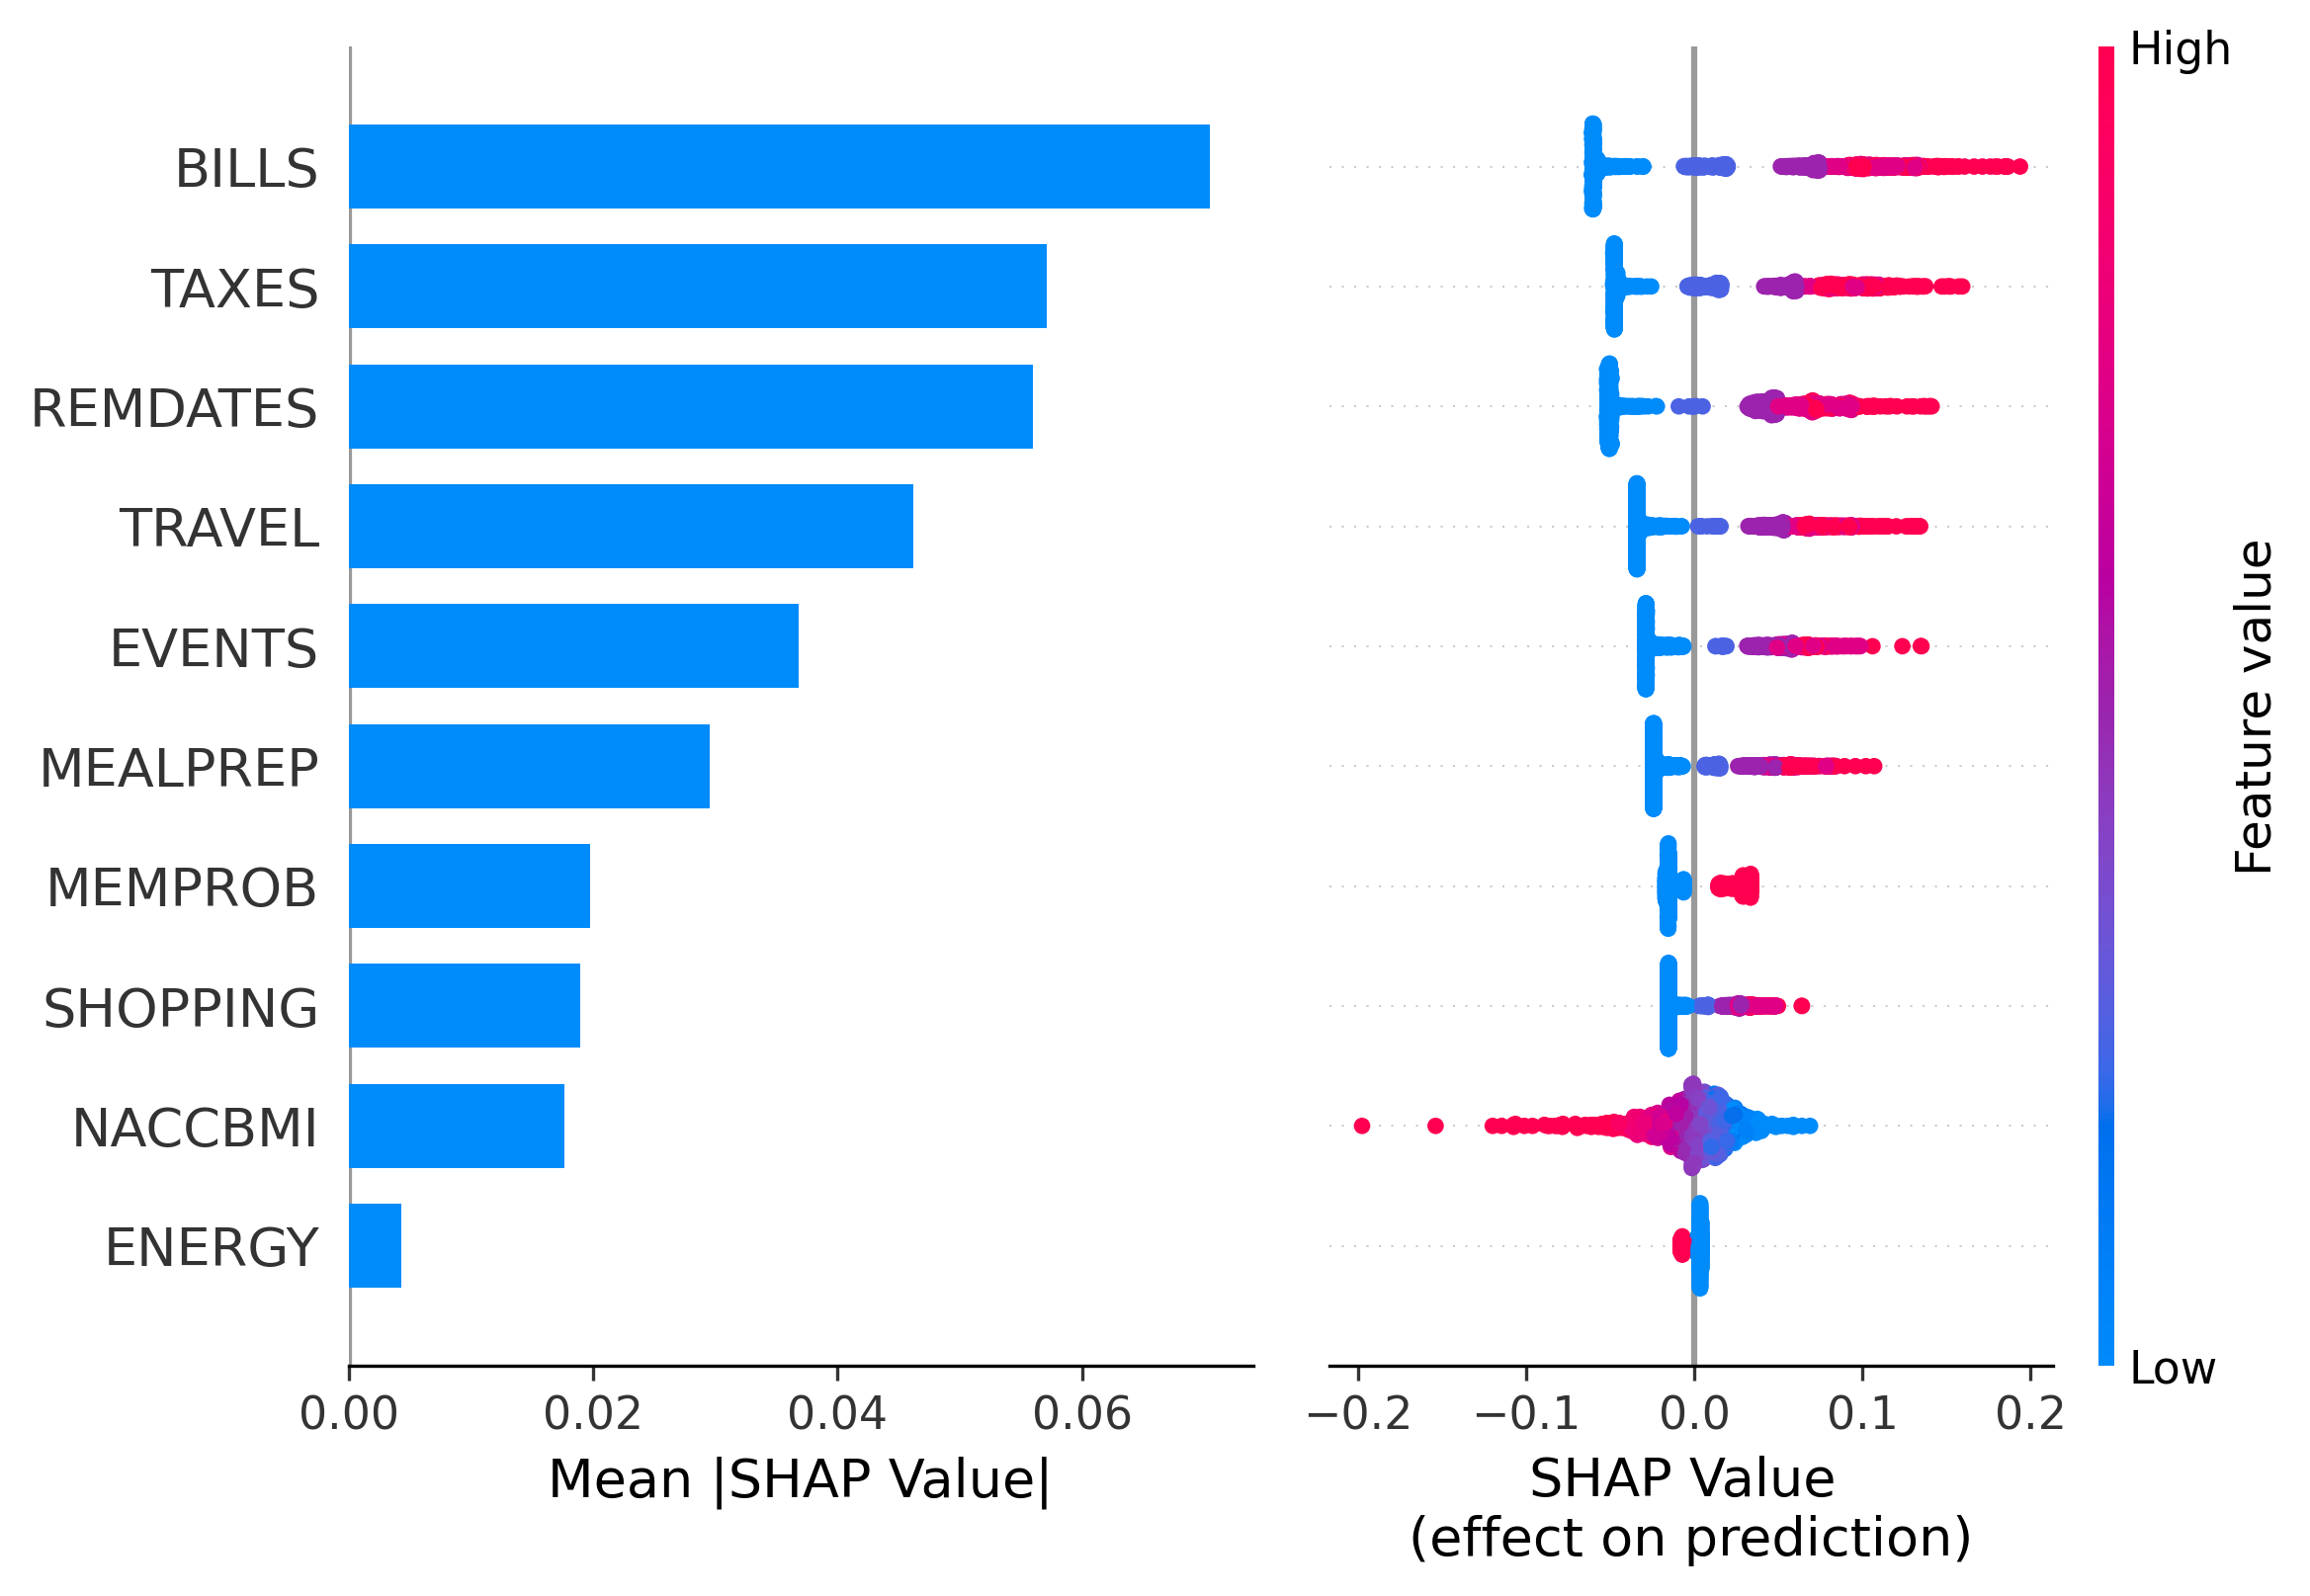
\includegraphics[width=\textwidth]{figures/appendix/dementia_prediction_nacc_shap_feature_importance.png}
        \caption*{(a)  NACC cross-center validation}
    \end{minipage}
    \begin{minipage}{0.48\textwidth}
        \centering
        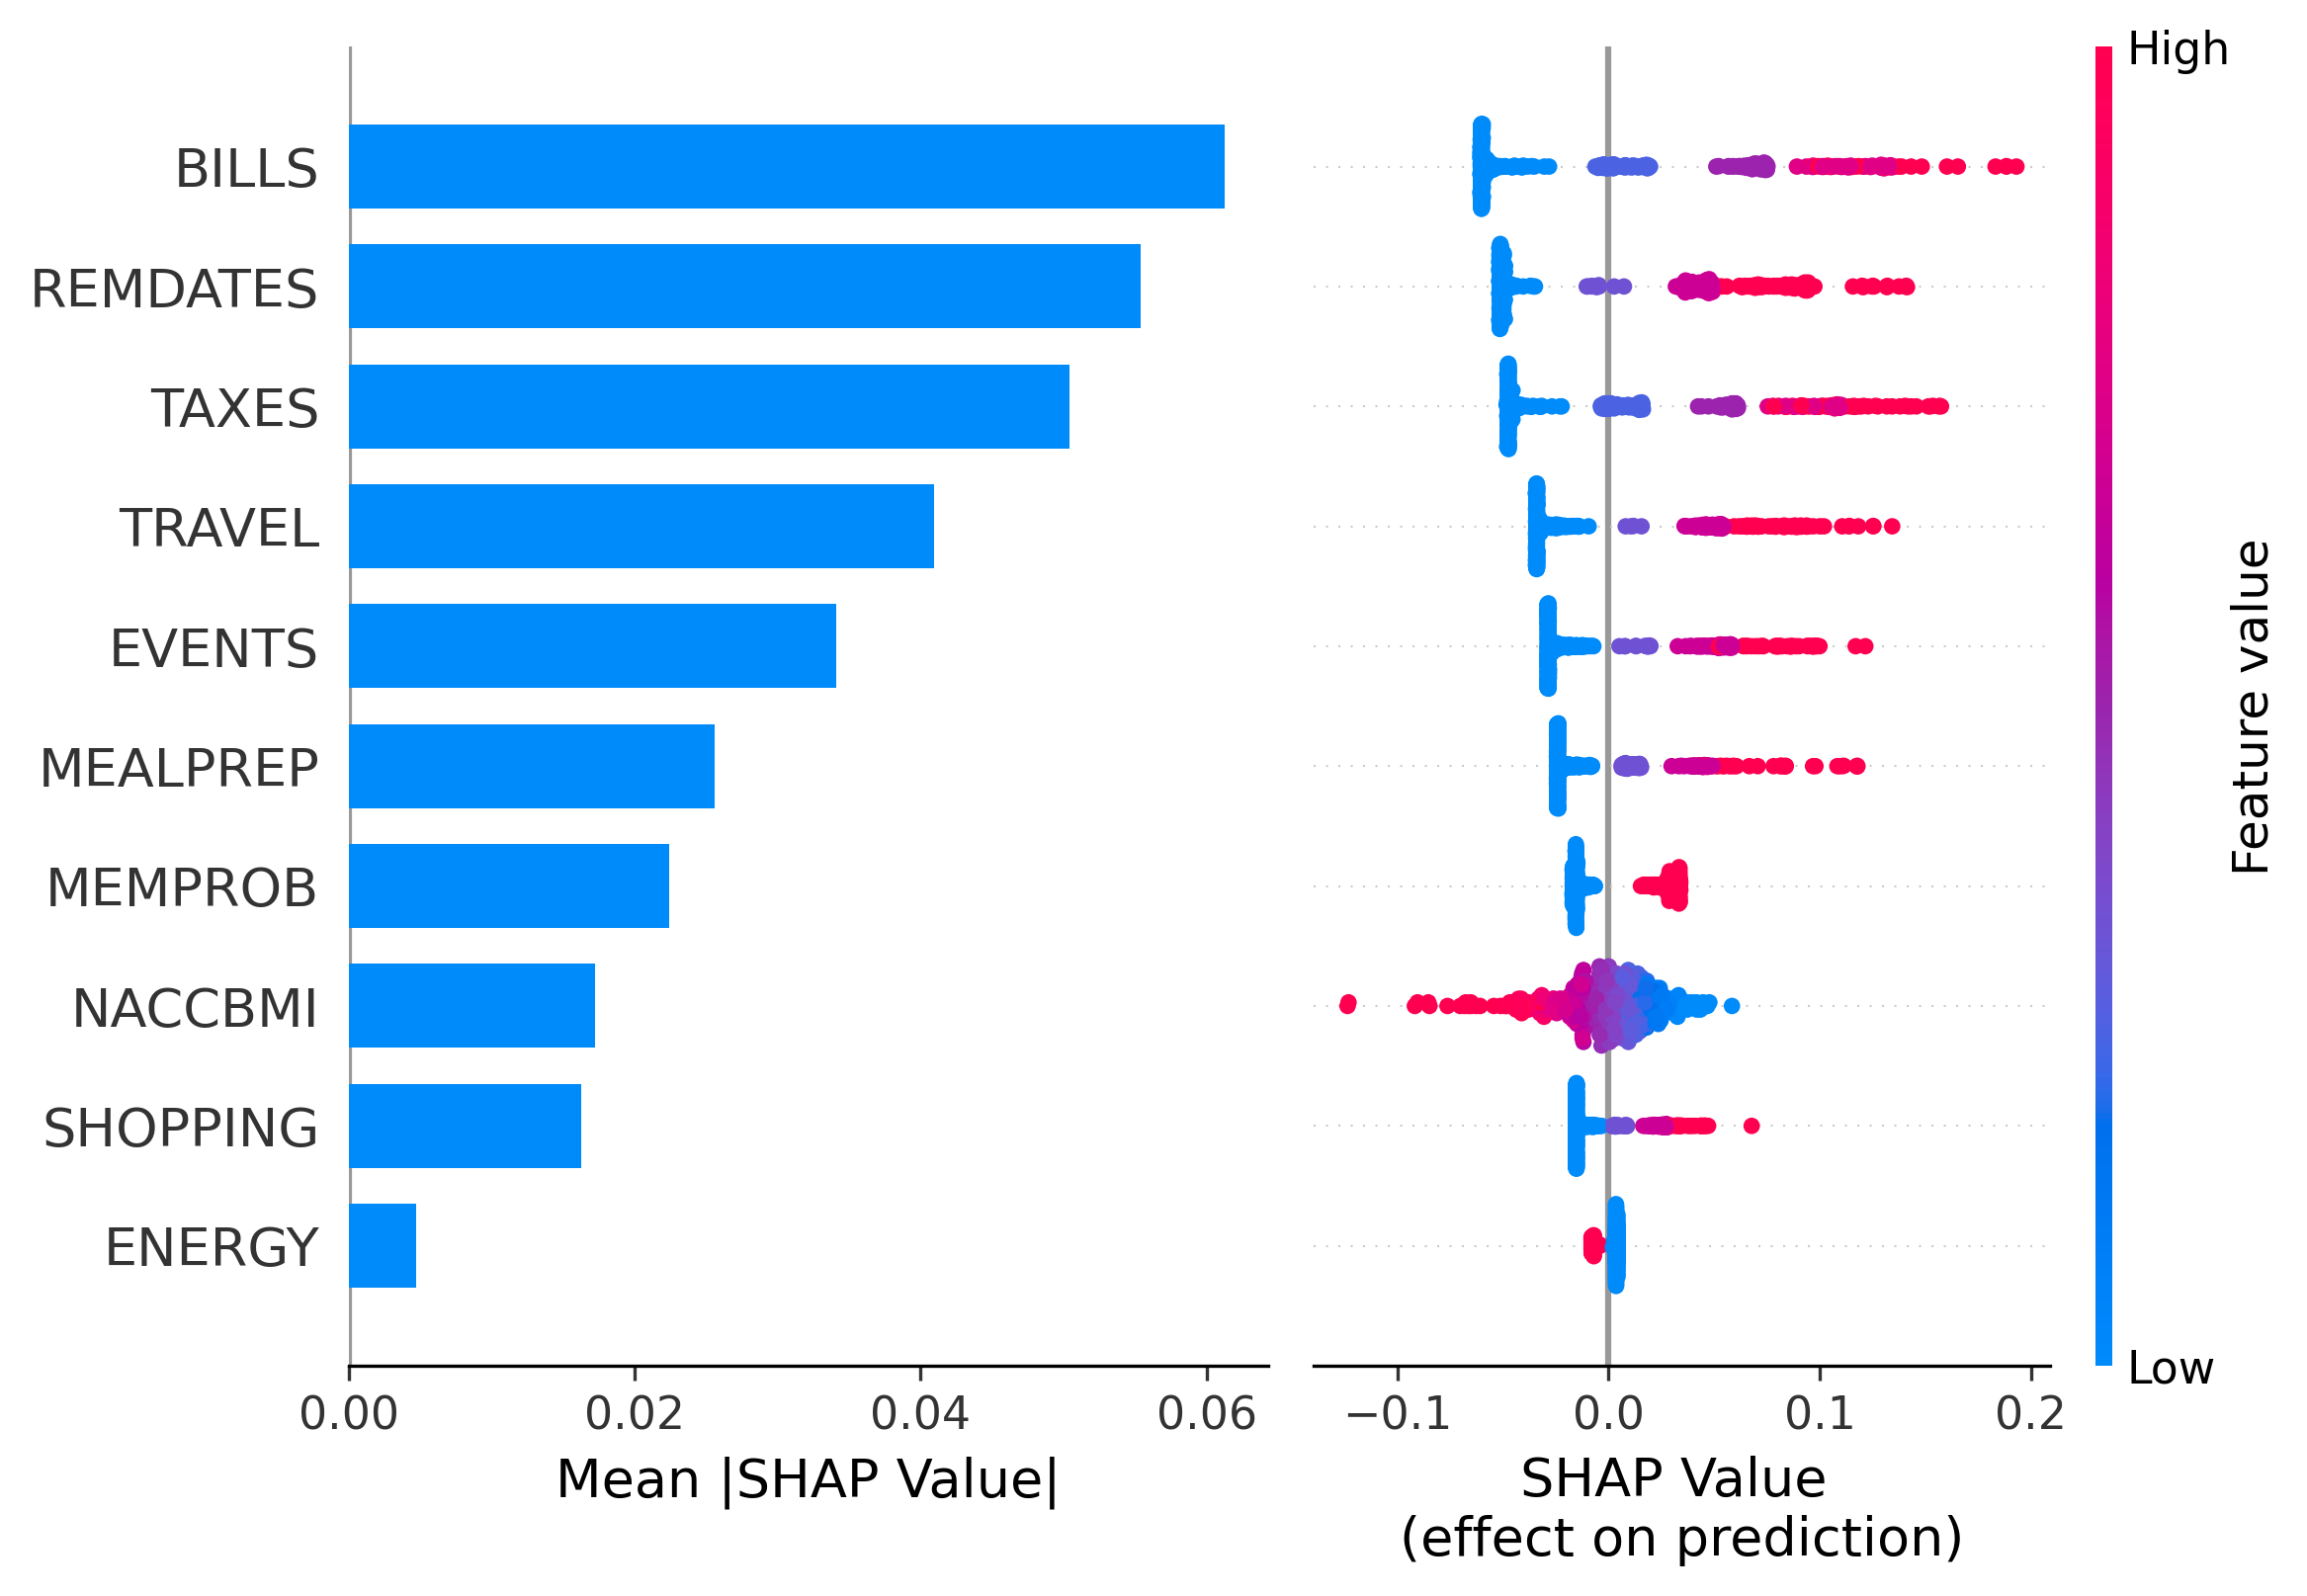
\includegraphics[width=\textwidth]{figures/appendix/dementia_prediction_adni_shap_feature_importance.png}
        \caption*{(b) ADNI External Validation}
    \end{minipage}
    \caption{Feature importance with summary plot for the feature CIND vs. dementia prediction task}
    \label{figure:summary-plot-task4-apdx}
\end{figure}

\begin{figure}[H]
    \centering
    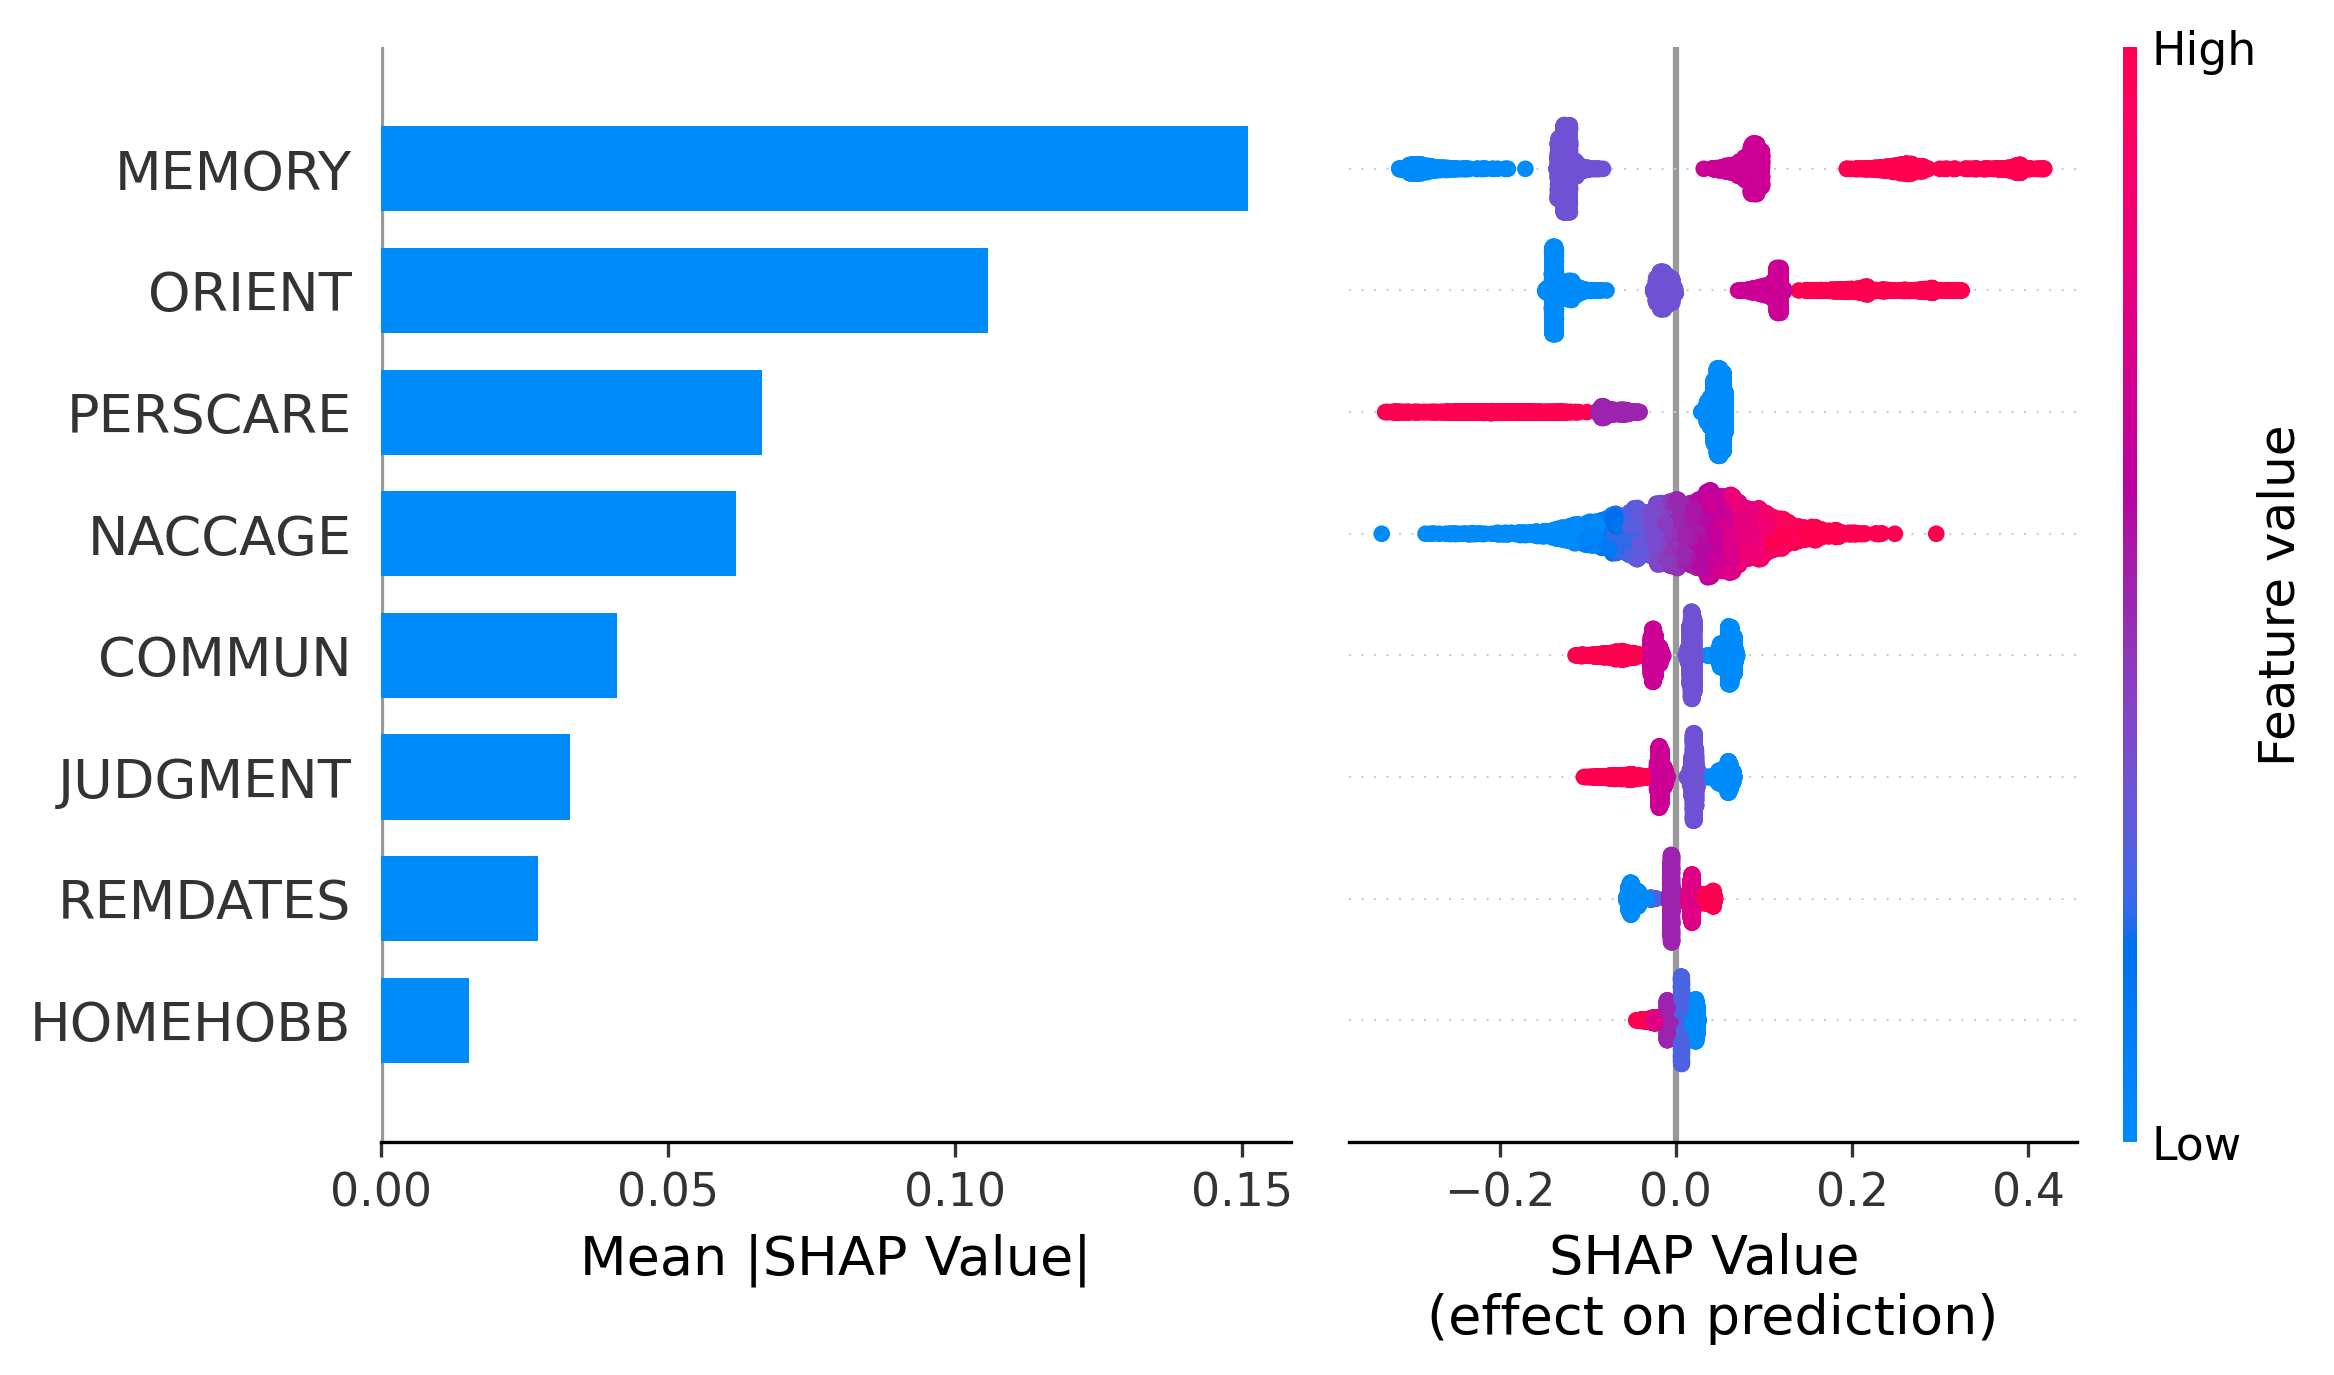
\includegraphics[width=0.7\textwidth]{figures/appendix/type_classification_nacc_shap_feature_importance.png}
    \caption{Feature importance with summary plot in the NACC cross-center validation for the AD vs. non-AD classification task}
    \label{figure:summary-plot-task5-apdx}
\end{figure}

% ----------------------------------------------------

\begin{figure}[H]
    \centering
    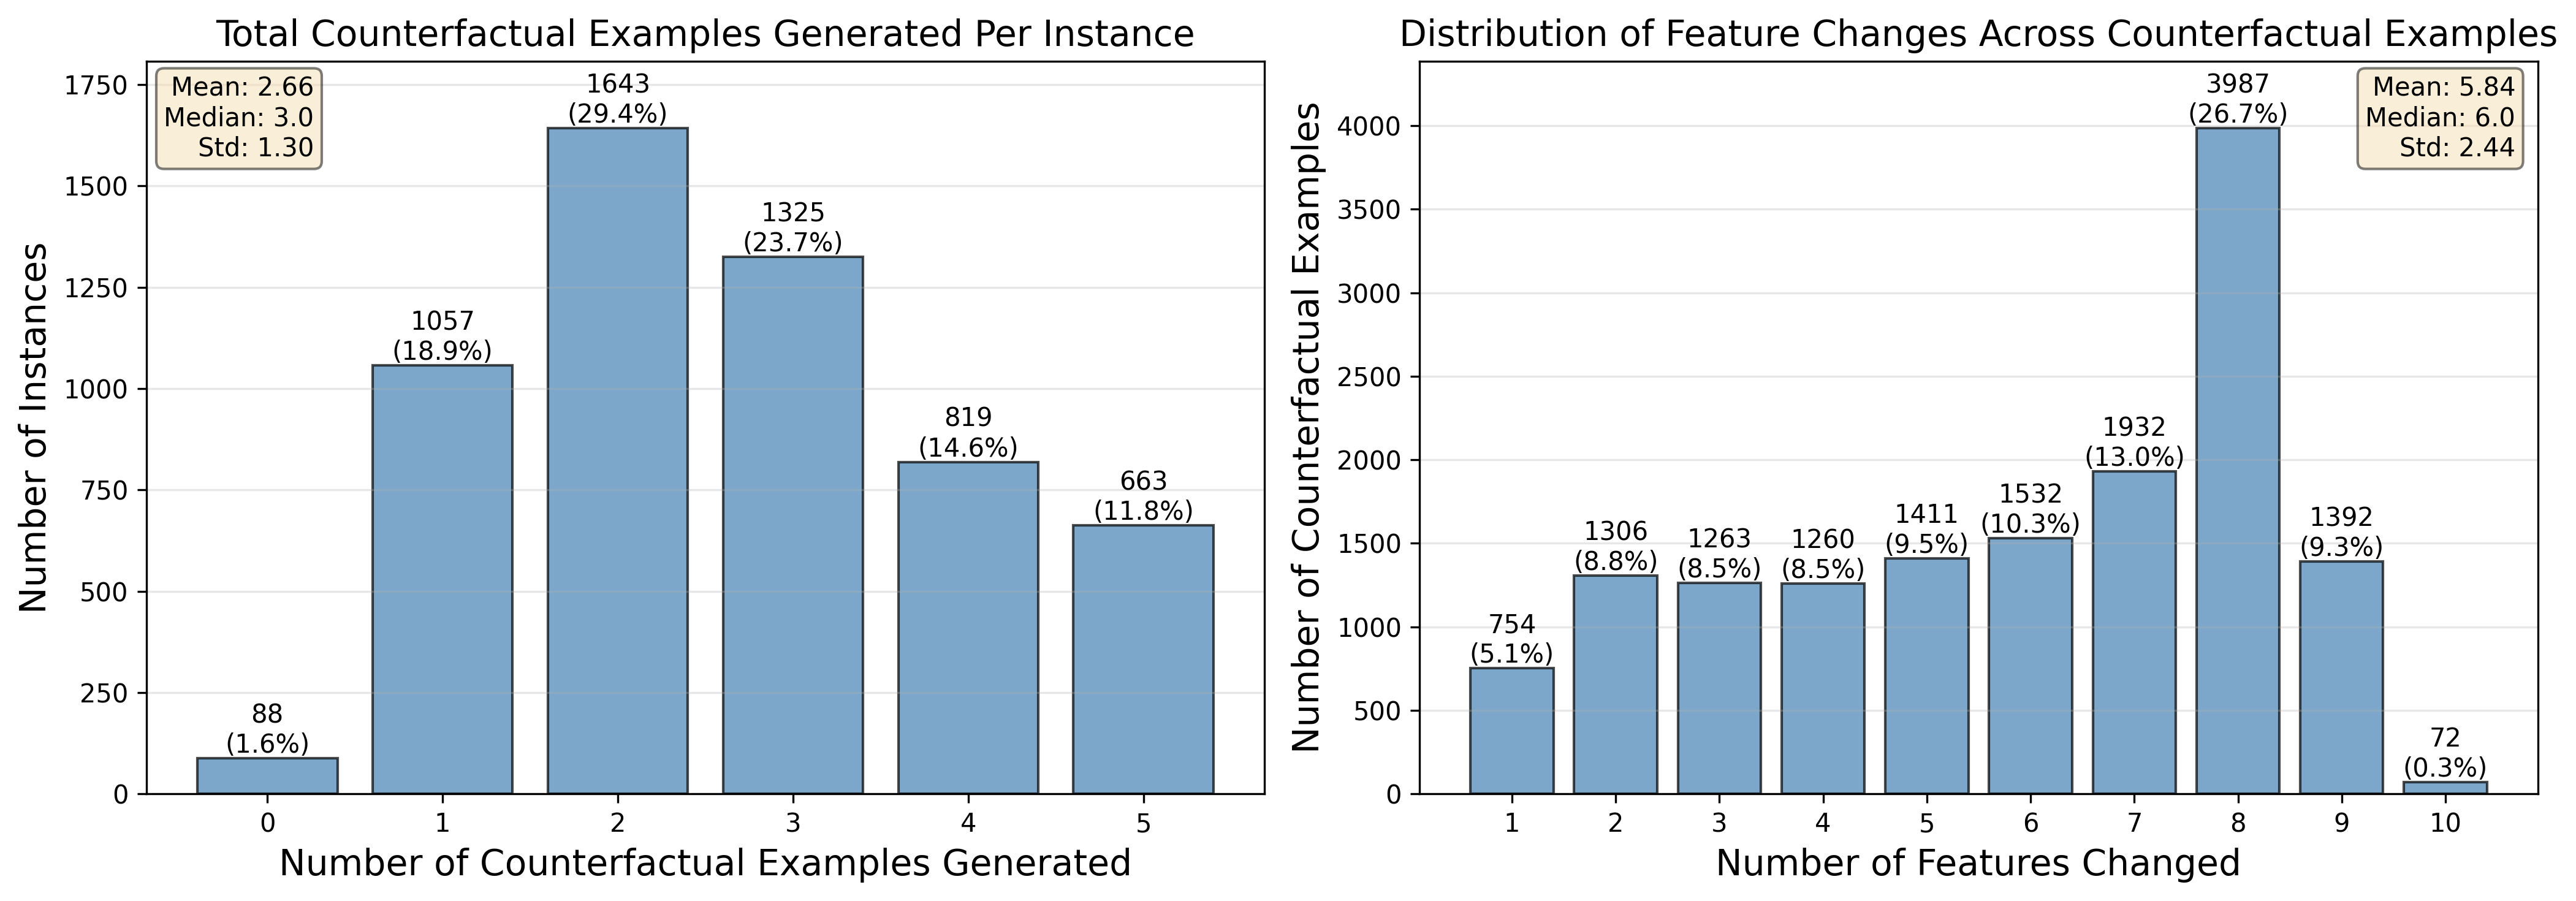
\includegraphics[width=\textwidth]{figures/appendix/impaired_classification_nacc_kdtree_dice_stats.png}
    \caption{Summary of generated counterfactual examples in the NACC cross-center validation for the NC vs. CI classification task}
    \label{figure:dice-nacc-task1-apdx}
\end{figure}

\begin{figure}[H]
    \centering
    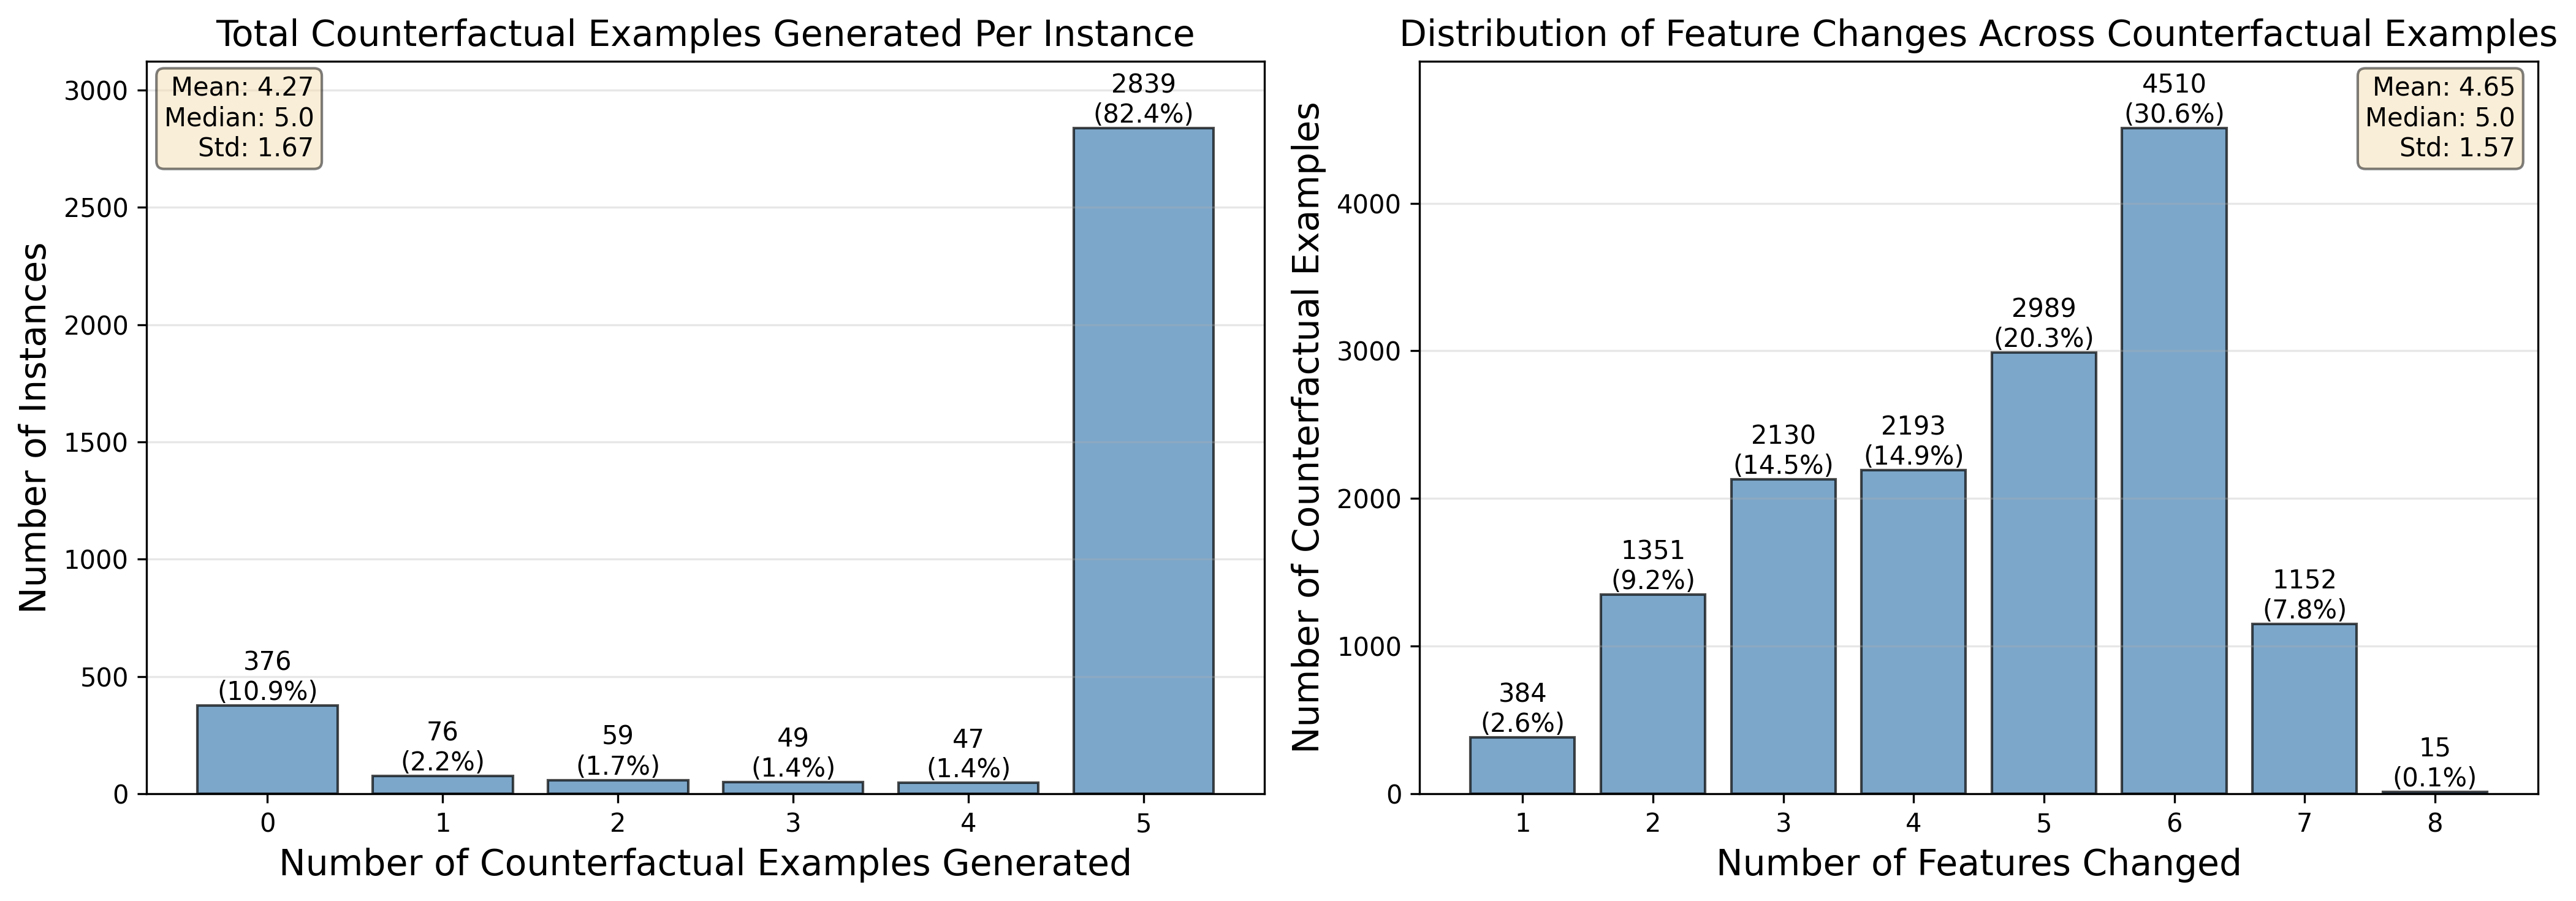
\includegraphics[width=\textwidth]{figures/appendix/dementia_classification_nacc_kdtree_dice_stats.png}
    \caption{Summary of generated counterfactual examples in the NACC cross-center validation for the CIND vs. dementia classification task}
    \label{figure:dice-nacc-task2-apdx}
\end{figure}

\begin{figure}[H]
    \centering
    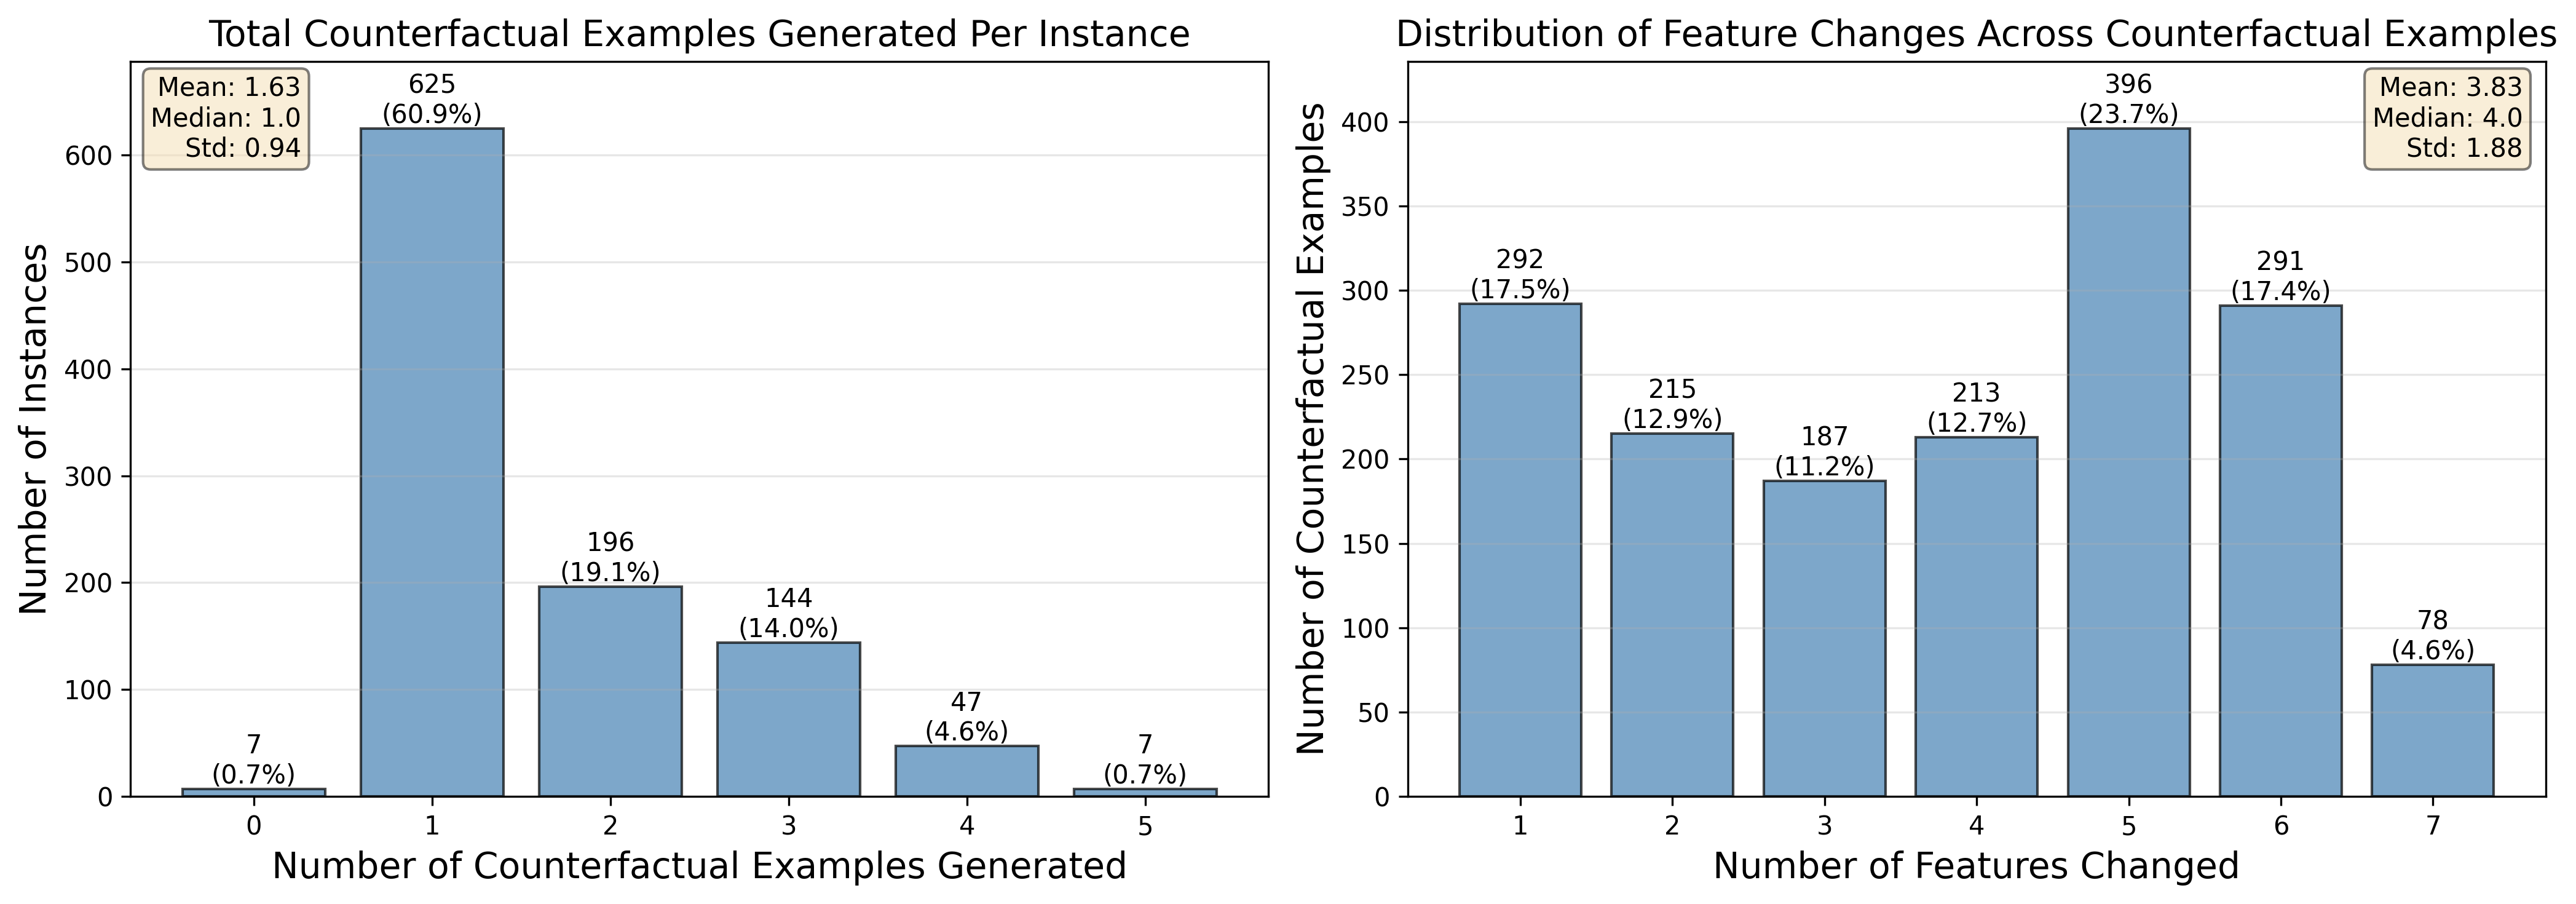
\includegraphics[width=\textwidth]{figures/appendix/impaired_prediction_nacc_kdtree_dice_stats.png}
    \caption{Summary of generated counterfactual examples in the NACC cross-center validation for the future NC vs. CI prediction task}
    \label{figure:dice-nacc-task3-apdx}
\end{figure}

\begin{figure}[H]
    \centering
    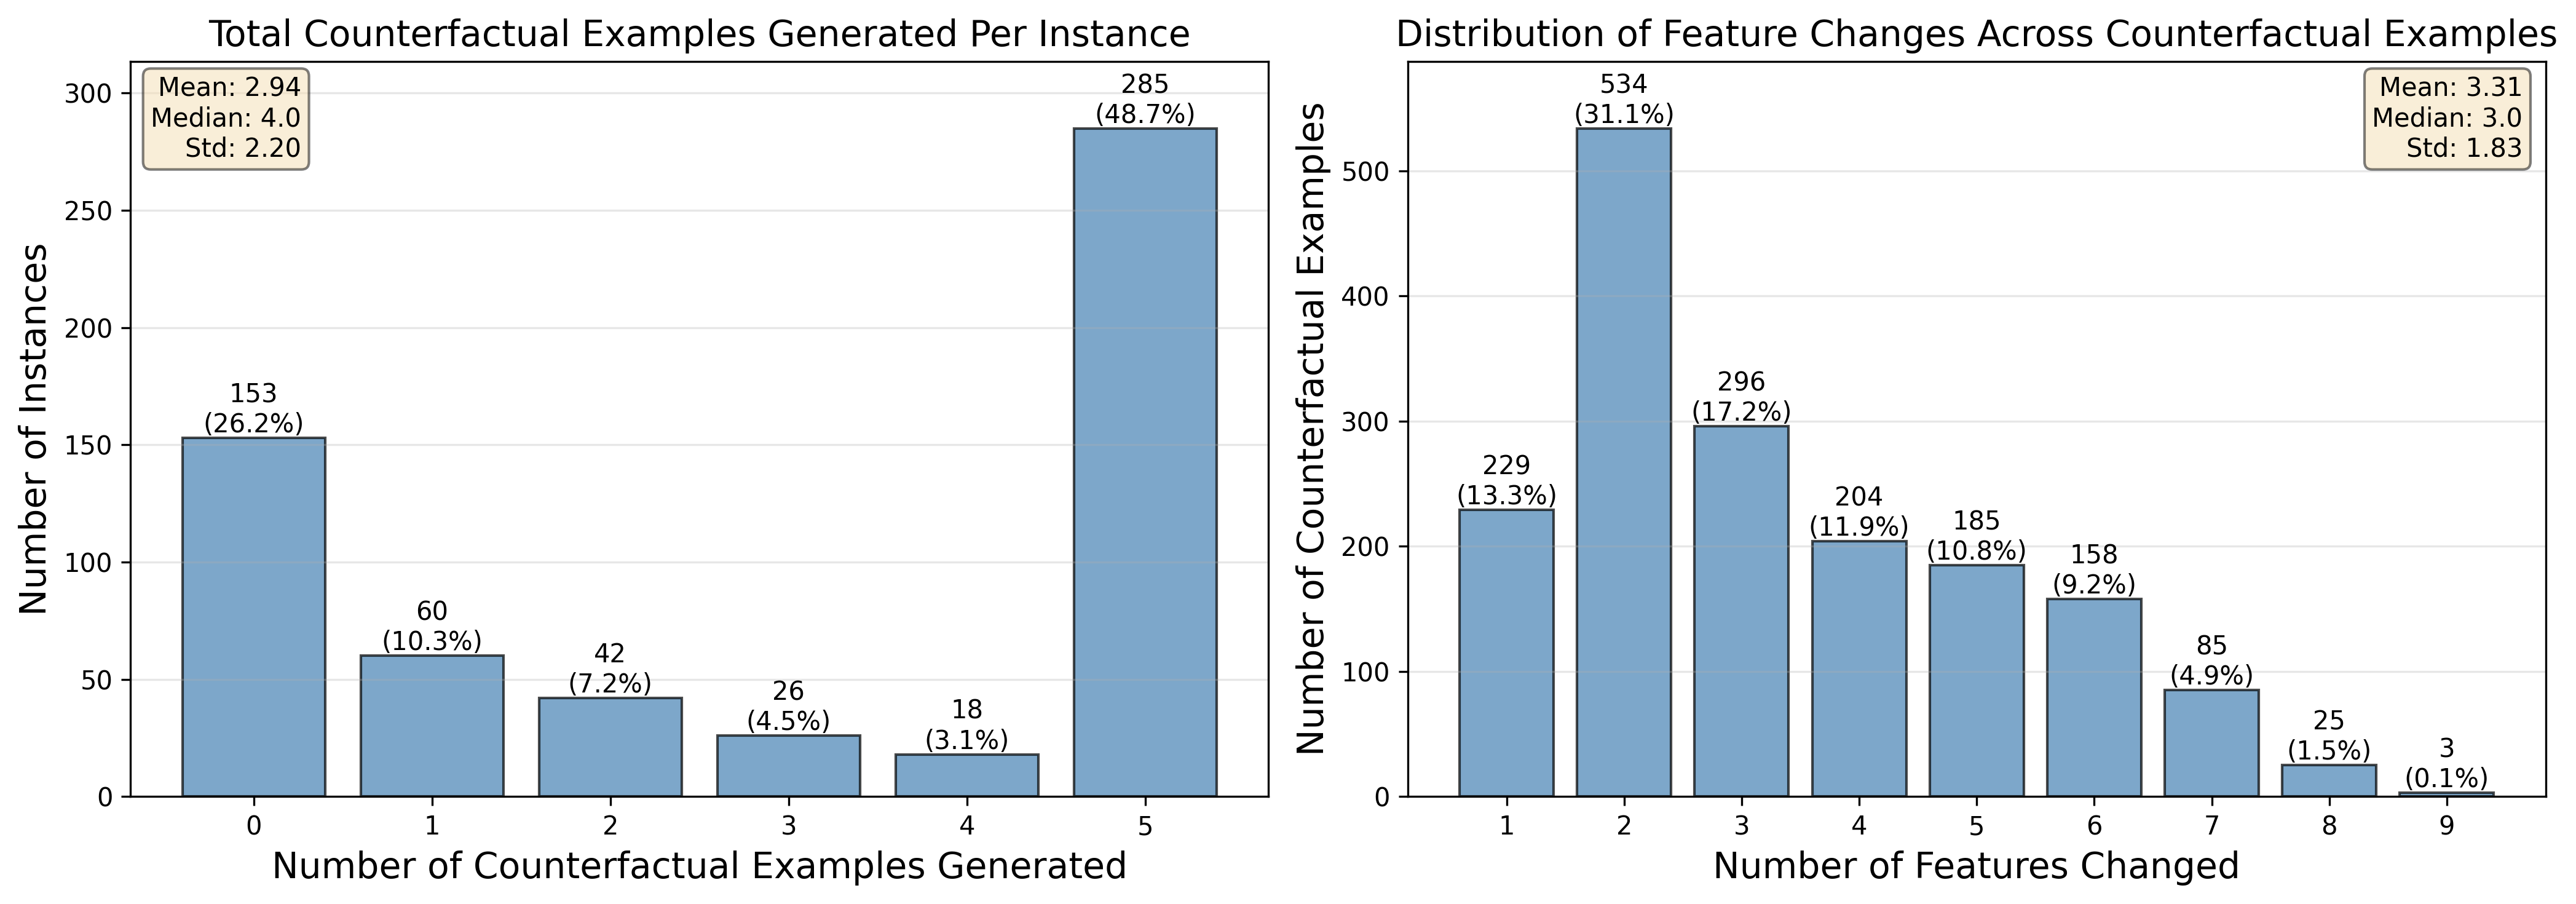
\includegraphics[width=\textwidth]{figures/appendix/dementia_prediction_nacc_random_dice_stats.png}
    \caption{Summary of generated counterfactual examples in the NACC cross-center validation for the future CIND vs.dementia prediction task}
    \label{figure:dice-nacc-task4-apdx}
\end{figure}

% ----------------------------------------------------

\begin{table}[H]
    \centering
    \caption{An illustration of counterfactual examples generated for a random subject classified as cognitive impairment (CI) to reverse the estimated outcome to normal cognition (NC)}
    \begin{tabular}{|c|c|c|c|c|}
    \hline
        \textbf{Feature} & \textbf{Original} & \textbf{CFE1} & \textbf{CFE2} & \textbf{CFE3} \\ \hline
        NACCAGE & 61 & ~ & ~ & ~ \\ \hline
        SEX & Male & ~ & ~ & ~ \\ \hline
        ANX & Yes & ~ & No & No \\ \hline
        MEMPROB & No & ~ & ~ & ~ \\ \hline
        BILLS & Normal & ~ & ~ & ~ \\ \hline
        TAXES & Normal & ~ & ~ & ~ \\ \hline
        SHOPPING & Normal & ~ & ~ & ~ \\ \hline
        GAMES & Normal & ~ & ~ & ~ \\ \hline
        EVENTS & Normal & ~ & ~ & ~ \\ \hline
        PAYATTN & Has difficulty & Normal & Normal & Normal \\ \hline
        REMDATES & Has difficulty & Normal & ~ & Normal \\ \hline
        TRAVEL & Has difficulty & Normal & Normal & ~ \\ \hline
        Outcome & CI & NC & NC & NC \\ \hline
    \multicolumn{5}{p{280pt}}{\footnotesize Empty cells indicate no change in feature values. Refer to Table~\ref{table:feature-details} for more details about the features. CFE: counterfactual examples.}
    \end{tabular}
    \label{table:cfe-adni-task1-apdx}
\end{table}

\begin{table}[H]
    \centering
    \caption{An illustration of counterfactual examples generated for a random subject classified as dementia to reverse the estimated outcome to cognitive impairment but not dementia (\acrshort{CIND})}
    \begin{tabular}{|c|c|c|c|c|}
    \hline
        \textbf{Feature} & \textbf{Original} & \textbf{CFE1} & \textbf{CFE2} & \textbf{CFE3} \\ \hline
        APP & Yes & ~ & ~ & No \\ \hline
        ENERGY & Yes & ~ & ~ & ~ \\ \hline
        BILLS & Requires assistance & Normal & ~ & Has difficulty \\ \hline
        TAXES & Dependent & ~ & Has difficulty & ~ \\ \hline
        SHOPPING & Normal & ~ & ~ & ~ \\ \hline
        GAMES & Normal & ~ & ~ & ~ \\ \hline
        MEALPREP & Normal & ~ & ~ & ~ \\ \hline
        EVENTS & Has difficulty & ~ & ~ & ~ \\ \hline
        REMDATES & Has difficulty & ~ & ~ & ~ \\ \hline
        TRAVEL & Dependent & Normal & Normal & Normal \\ \hline
        PRIMLANG & English & ~ & ~ & ~ \\ \hline
        Outcome & dementia & CIND & CIND & CIND \\ \hline
    \multicolumn{5}{p{350pt}}{\footnotesize Empty cells indicate no change in feature values. Refer to Table~\ref{table:feature-details} for more details about the features. CFE: counterfactual examples.}
    \end{tabular}
    \label{table:cfe-adni-task2-apdx}
\end{table}

\begin{table}[H]
    \centering
    \caption{An illustration of counterfactual examples generated for a random subject with a future risk of cognitive impairment (CI) to reverse the estimated outcome to normal cognition (NC)}
    \begin{tabular}{|c|c|c|c|c|}
    \hline
        \textbf{Feature} & \textbf{Original} & \textbf{CFE1} & \textbf{CFE2} & \textbf{CFE3} \\ \hline
        NACCAGE & 64 & ~ & ~ & ~ \\ \hline
        SEX & Female & ~ & ~ & ~ \\ \hline
        IRR & Yes & ~ & No & No \\ \hline
        MEMPROB & No & ~ & ~ & ~ \\ \hline
        BILLS & Normal & ~ & ~ & ~ \\ \hline
        TAXES & Normal & ~ & ~ & ~ \\ \hline
        SHOPPING & Normal & ~ & ~ & ~ \\ \hline
        REMDATES & Requires assistance & Normal & Normal & Has difficulty \\ \hline
        TRAVEL & Has difficulty & Normal & ~ & Normal \\ \hline
        Outcome & CI & NC & NC & NC \\ \hline
    \multicolumn{5}{p{350pt}}{\footnotesize Empty cells indicate no change in feature values. Refer to Table~\ref{table:feature-details} for more details about the features. CFE: counterfactual examples.}
    \end{tabular}
    \label{table:cfe-adni-task3-apdx}
\end{table}

\begin{table}[H]
    \centering
    \caption{An illustration of counterfactual examples generated for a random subject with a future risk of dementia to reverse the estimated outcome to cognitive impairment but not dementia (\acrshort{CIND})}
    \begin{tabular}{|c|c|c|c|c|}
    \hline
        \textbf{Feature} & \textbf{Original} & \textbf{CFE1} & \textbf{CFE2} & \textbf{CFE3} \\ \hline
        NACCBMI & 29.0 & ~ & ~ & 22.6 \\ \hline
        MEMPROB & Yes & No & ~ & ~ \\ \hline
        ENERGY & Yes & No & ~ & ~ \\ \hline
        BILLS & Normal & ~ & ~ & ~ \\ \hline
        TAXES & Has difficulty & ~ & ~ & Normal \\ \hline
        SHOPPING & Normal & ~ & ~ & ~ \\ \hline
        MEALPREP & Never did & ~ & ~ & ~ \\ \hline
        EVENTS & Normal & ~ & ~ & ~ \\ \hline
        REMDATES & Has difficulty & ~ & Normal & ~ \\ \hline
        TRAVEL & Normal & ~ & ~ & ~ \\ \hline
        Outcome & dementia & CIND & CIND & CIND \\ \hline
    \multicolumn{5}{p{280pt}}{\footnotesize Empty cells indicate no change in feature values. Refer to Table~\ref{table:feature-details} for more details about the features. CFE: counterfactual examples.}
    \end{tabular}
    \label{table:cfe-adni-task4-apdx}
\end{table}

\section{Summary of the Comparative Analysis with Existing Literature}\label{sec:compare-summary-apdx}
This section provides a summary of the comparison between this study and the reviewed studies discussed in Section~\ref{sec:performance-comparison}. The comparison in Table~\ref{table:compare-summary} is presented across the main dimensions of methodological quality that affect the reliability, the cost-effectiveness, and the clinical utility of the developed models.

\setlength{\tabcolsep}{4pt}
\begin{longtable}{|M{0.18\textwidth}|M{0.40\textwidth}|M{0.06\textwidth}|M{0.06\textwidth}|M{0.06\textwidth}|M{0.06\textwidth}|M{0.06\textwidth}|}
\caption{Summary of the comparative analysis between this study and the reviewed literature across the main dimensions of methodological quality}
\label{table:compare-summary} \\
\hline
\textbf{Study} & \textbf{Key Features} & \rh{External Validation} & \rh{Calibration / DCA} & \rh{Class Imbalance Handling} & \rh{Class Overlap Analysis} & \rh{Computational Cost} \\
\hline
\endfirsthead

\caption[]{Summary of the comparative analysis between this study and the reviewed literature, continued} \\
\hline
\textbf{Study} & \textbf{Key Features} & \rh{External Validation} & \rh{Calibration / DCA} & \rh{Class Imbalance Handling} & \rh{Class Overlap Analysis} & \rh{Computational Cost} \\
\hline
\endhead

\hline
\multicolumn{7}{r}{\textit{Continued on next page}} \\
\endfoot

\hline
\multicolumn{7}{p{\textwidth}}{\footnotesize ADL: activities of daily living; CDR: clinical dementia rating; DCA: decision curve analysis; EHR: electronic health records; IADL: instrumental activities of daily living; MMSE: Mini-Mental State Examination. The check mark (\yesmark) indicates that the dimension was addressed or reported, the cross (\nomark) indicates that it was not, and the dash (\partialmark) indicates a partial case. In the external validation column, a partial case refers to a prospective validation on the same cohort rather than a separate external dataset, while in the computational cost column it refers to a study that reported only the computation time of the model.} \\
\endlastfoot

\textbf{This Study} & Demographic, functional (IADL); CDR for subtype & \yesmark & \yesmark & \yesmark & \yesmark & \yesmark \\
\hline
\cite{Gurevich2017Neuropsychological} & Demographic, neuropsychological tests & \nomark & \nomark & \nomark & \nomark & \nomark \\
\hline
\cite{Ben2020Predicting} & EHR: diagnoses, medications, notes & \nomark & \nomark & \nomark & \nomark & \nomark \\
\hline
\cite{Park2020Machine} & Claims and EHR: labs, diagnoses, medications & \nomark & \nomark & \nomark & \nomark & \nomark \\
\hline
\cite{Davoudi2021Classifying} & Digital clock-drawing test & \nomark & \nomark & \nomark & \nomark & \nomark \\
\hline
\cite{Yamada2022Characteristics} & Drawing-test features & \nomark & \nomark & \nomark & \nomark & \nomark \\
\hline
\cite{Maito2022Classification} & Cognitive and social-cognition tests & \nomark & \nomark & \yesmark & \nomark & \nomark \\
\hline
\cite{Pang2023Predicting} & Demographic, neuropsychological tests, CDR & \nomark & \nomark & \nomark & \nomark & \nomark \\
\hline
\cite{Li2023Early} & EHR: diagnoses, medications, labs, vitals & \nomark & \nomark & \nomark & \nomark & \nomark \\
\hline
\cite{Li2023Machine} & Demographic, lifestyle, labs, cognitive tests & \nomark & \yesmark & \nomark & \nomark & \nomark \\
\hline
\cite{Bucholc2023Hybrid} & Cognitive and functional tests & \nomark & \nomark & \yesmark & \nomark & \nomark \\
\hline
\cite{Twait2023Dementia} & Demographic, lifestyle, MMSE & \nomark & \yesmark & \yesmark & \nomark & \nomark \\
\hline
\cite{Ren2023Improving} & Demographic, history, MMSE & \nomark & \nomark & \yesmark & \nomark & \nomark \\
\hline
\cite{Yue2023Explainable} & Demographic, lifestyle, history & \nomark & \nomark & \yesmark & \nomark & \partialmark \\
\hline
\cite{abbas2024Explainable} & Demographic, history, CDR & \yesmark & \nomark & \nomark & \nomark & \nomark \\
\hline
\cite{Cui2024Prediction} & Demographic, health, ADL and IADL & \yesmark & \yesmark & \nomark & \nomark & \nomark \\
\hline
\cite{Sharma2024Leveraging} & Demographic, comorbidities & \nomark & \nomark & \yesmark & \nomark & \nomark \\
\hline
\cite{Oh2024Multivariable} & Sociodemographic, health, functional & \nomark & \nomark & \yesmark & \nomark & \nomark \\
\hline
\cite{Georgiev2024Predicting} & Demographic, lifestyle, labs, frailty index & \nomark & \yesmark & \nomark & \nomark & \nomark \\
\hline
\cite{Richter2025Cognitive} & Sociodemographic, labs, comorbidities, functional & \nomark & \nomark & \yesmark & \nomark & \nomark \\
\hline
\cite{Akter2025Using} & EHR: vitals, comorbidities & \nomark & \nomark & \nomark & \nomark & \nomark \\
\hline
\cite{Ren2025Using} & Demographic, lifestyle, blood biomarkers, MMSE & \partialmark & \nomark & \yesmark & \nomark & \nomark \\
\hline
\cite{Ye2025Predicting} & Demographic, IADL, social participation & \nomark & \nomark & \nomark & \nomark & \nomark \\
\hline

\end{longtable}
\setlength{\tabcolsep}{6pt}
%!TEX ROOT = thesis.tex
%to not listed in ToC
\addtocontents{toc}{\protect\setcounter{tocdepth}{-1}}

\chapter{Glossary}

\hspace{4em}%for indentation

\begin{longtable}{|M{3cm}|M{9.5cm}|}

    \caption{Glossary of key terms and concepts used in this study}

    \\ \hline
    \textbf{Term} & \textbf{Definition}
    \\ \hline
    \endfirsthead

    \caption[]{Glossary of key terms and concepts used in this study, continued}
    \\ \hline
    \textbf{Term} & \textbf{Definition}
    \\ \hline                        
    \endhead
 
    \hline
    \endfoot
        Accessible Data & Data that can be easily collected from subjects or their caregivers during a primary care visit at minimal or no cost, such as demographics, medical history, behavioral surveys, and functional assessments. \\ \hline
        Baseline Visit & The initial data collection point (visit) used as the reference for predicting cognitive status at a future time (e.g., five years later). \\ \hline
        Benchmark Model & A baseline machine learning model with the best performance out of other models in the hyperparameter optimization process. It is used by the proposed Model Selection Algorithm for comparison to identify the most cost-effective model. \\ \hline
        Beta Calibration & A method used to align the predicted probabilities of a model with the actual likelihood of the risk, capable of correcting both overconfidence and underestimation. \\ \hline
        Brier Score & A metric used to evaluate the accuracy of probabilistic predictions, where a lower score indicates better calibration and reliability of the predicted probabilities. \\ \hline
        Class Imbalance & A condition in datasets where the number of instances in one class (typically normal cognition) significantly exceeds the number of instances in others (e.g., dementia), often leading to biased model predictions. \\ \hline
        Class Overlap & A challenge in classification where different classes share similar characteristics or feature values, making them difficult to separate in the feature space. \\ \hline
        Classification Task & The specific modeling objective of identifying a subject's current cognitive status (e.g., Normal Cognition vs. Cognitive Impairment) using data from the same visit. \\ \hline
        Cognitive Impairment (CI) & A medical condition described as a limitation of the human brain to function normally, limiting the patient's ability to think, remember, pay attention, communicate, solve problems, and make decisions. \\ \hline
        Cognitive Status & The clinical diagnostic category characterizing a subject's cognitive function, classified in this study as Normal Cognition (NC), Cognitive Impairment but not Dementia (CIND), or Dementia. \\ \hline
        Cost-effective Model & An accurate and efficient prediction model developed using accessible screening tools and data that avoids expensive equipment, making it suitable for resource-constrained settings. \\ \hline
        Cost-effective Model Selection Algorithm & A novel algorithm developed in this study that selects the best model by balancing performance metrics with training and prediction throughputs (speed). \\ \hline
        Counterfactual Examples & Specific, generated hypothetical instances that demonstrate the minimal changes required in a subject's data (e.g., reducing a depression score) to alter the model's prediction from "high risk" to "low risk". \\ \hline
        Counterfactual Explanations & An XAI method that offers actionable insights by suggesting minimal changes in a patient's data (e.g., lowering a depression score) that would result in a different model prediction. \\ \hline
        Decision Curve Analysis (DCA) & A method to evaluate the clinical utility of a model by calculating its net benefit across different probability thresholds, comparing it against "treat all" and "treat none" strategies. \\ \hline
        Dementia & A severe decline in cognitive functions that makes patients rely on others to perform their daily tasks. \\ \hline
        Expected Calibration Error (ECE) & A summary statistic that measures the difference between the model's predicted probabilities and the actual outcome frequencies; lower values indicate better calibration. \\ \hline
        Explainability & The capability of a machine learning model to provide transparent and human-understandable insights into its decision-making process, ensuring that predictions are trustworthy and can be translated into actionable clinical recommendations. \\ \hline
        Explainable Artificial Intelligence (XAI) & An interpretable approach integrated into machine learning models to describe how they make predictions and which input features drive the outcome. \\ \hline
        External Validation & The process of testing a machine learning model on an independent dataset collected from a different population or setting than the training data to assess its generalizability. \\ \hline
        Feature Overlap & A type of class overlap where the distribution of values for individual features is similar across different classes, resulting in low discriminative power. \\ \hline
        Generalizability & The extent to which the research findings can be applied to settings, situations, or groups other than those that were originally studied. \\ \hline
        Hierarchical Classification Strategy & A strategy that decomposes a complex classification problem into smaller binary tasks (e.g., Normal vs. Impaired, then Mild Impaired vs. Dementia) to improve performance and clinical utility. \\ \hline
        Hybrid Data Resampling & A data preprocessing approach utilized in this study that combines cleaning-based methods (like ENN) and oversampling methods (like BorderlineSMOTE) to handle class imbalance and overlap. \\ \hline
        Instance-Level Overlap & A type of class overlap occurring when individual data points from different classes are located in close proximity or mixed within the feature space (e.g., borderline points). \\ \hline
        Internal Validation & Evaluating a model's performance using a subset of the same dataset used for training (e.g., k-fold cross-validation). \\ \hline
        Interpretability & The extent to which a human can understand the reasoning behind a model's decision; often used interchangeably with explainability to describe the transparency of "white-box" or explained models. \\ \hline
        NACC Cross-center Validation & A specific external validation strategy where models trained on data from one set of research centers are tested on unseen data from different centers within the NACC dataset to assess generalizability. \\ \hline
        Prediction Task & The modeling objective of forecasting a subject's future cognitive status over a specified period (e.g., 5 years) using data from the baseline visit. \\ \hline
        Prediction Throughput & The total number of predictions a model can make per second, used as a measure of model efficiency. \\ \hline
        Structural Overlap & A type of class overlap related to the geometric complexity of the decision boundary between classes. \\ \hline
        Subjects & The individuals (participants) included in the study cohorts (NACC and ADNI) whose data are used for training and validating the models. \\ \hline
        Training Throughput & The total number of samples a model can learn per second, used as a measure of model efficiency. \\ \hline
        Treat All & A baseline strategy in Decision Curve Analysis assuming all subjects are predicted to have the condition (e.g., Cognitive Impairment). \\ \hline
        Treat None & A baseline strategy in Decision Curve Analysis assuming none of the subjects are predicted to have the condition. \\ \hline
   
\end{longtable}
\end{appendices}
% resume the ToC depth
\addtocontents{toc}{\protect\setcounter{tocdepth}{3}}
\addtocontents{toc}{\protect\vspace{16pt}}


\backmatter
\ownpubs
\nocitejour{Shubar2024Optimizing}
\bibliographyjour{references}
\bibliographyconf{references}

\end{document}